\documentclass[a4paper, 11pt]{article}



%%%%%%%%%%%%%%%%%%%%%%%%%%%%%%%%%
%	 PACKAGES	%
%%%%%%%%%%%%%%%%%%%%%%%%%%%%%%%%%
% Codierung von in und Output
\usepackage[utf8]{inputenc}
\usepackage[T1]{fontenc}

% AMS-Pakete für Mathe
\usepackage{amsthm,amssymb,amsmath}
\usepackage{cancel} %Durchgestrichene Symbole

% Sprachpaket neue rechtschreibung
\usepackage[ngerman]{babel}


\usepackage[most]{tcolorbox}

%Header und Seitengrösse
\usepackage{fancyhdr}
\usepackage{geometry}

% Paket für Links im PDF (glaubs)!
\usepackage[hidelinks]{hyperref}

%Paket um ganze pdf-File zu importieren (Arbeitsblätter aus Analysis DMK)
\usepackage{pdfpages}

%TColorbox nutzt Theoreme und bessere Verweise
\tcbuselibrary{theorems}
\usepackage{cleveref}
\crefname{section}{Kapitel}{Kapitel}
\Crefname{section}{Kapitel}{Kapitel}

%Package, um Aufgaben auf mehrere Spalten zu verteilen.
\usepackage{tasks}

%Tikz
\usepackage{tikz}
\usepackage{pgfplots}
\pgfplotsset{compat=1.18}




%Programmcode-Darstellung
\usepackage{listings}
\usepackage{xcolor}
\lstset{basicstyle=\ttfamily}
\definecolor{codekeyword}{rgb}{0.11,0.53,0.63}
\definecolor{codenumbers}{rgb}{0.71,0.21,0.30}
\definecolor{codeoperation}{rgb}{0.57,0.32,0.59}
\definecolor{codecomment}{rgb}{0.17,0.59,0.28}
\definecolor{backcolour}{rgb}{0.98,0.97,0.99}
\definecolor{codestring}{rgb}{0.84,0.56,0.16}
\lstdefinestyle{mystyle}{
	backgroundcolor=\color{backcolour},
	commentstyle=\color{codecomment},
	keywordstyle=\color{codekeyword},
	numberstyle=\tiny\color{black},
	stringstyle=\color{codestring},
	basicstyle=\ttfamily\footnotesize,
	breakatwhitespace=false,
	breaklines=true,
	captionpos=b,
	keepspaces=true,
	numbers=left,
	numbersep=5pt,
	showspaces=false,
	showstringspaces=false,
	showtabs=false,
	tabsize=4
}

\lstset{style=mystyle}







% kein Plan, was das folgende macht... :(
% \lstset{basicstyle=\ttfamily}
% \makeatletter
% \def\BState{\State\hskip-\ALG@thistlm}
% \makeatother

\usepackage{graphicx}
\usepackage{hyperref}
\usepackage{array}
\hypersetup{colorlinks=true}

% damit kann man nummerierte Liste unterbrechen und wieder aufnehmen
\usepackage{enumitem}

%%%CHANGE LABEL FIGURE
\usepackage[figurename=Abbildung.]{caption}

%%%%%%%%%%%%%%%%%%%%%%%%%%%%%%%%
%%%%%%%%%%%	LAYOUT	%%%%%%%%%%%%
%%%%%%%%%%%%%%%%%%%%%%%%%%%%%%%%

\geometry{
	a4paper,
	total={165mm,225mm},
	left=25mm,
	top=35mm,
}

%keine Einrückung bei Absatz dafür Abstand
\setlength\parindent{0pt}
\setlength{\parskip}{1em}

%Header
\pagestyle{fancy}
\setlength{\headheight}{13.6pt}
\renewcommand{\sectionmark}[1]{ \markright{#1}{} }
\lhead[L]{M. Anderegg}
\chead{}
\rhead{Analysis~--~\rightmark}
\lfoot{}
\cfoot{\thepage}
\rfoot{}





%%%%%%%%%%%%%%%%%%%%%%%%%%%%%%%%
%%%%%%%%% TCB-Commands %%%%%%%%%
%%%%%%%%%%%%%%%%%%%%%%%%%%%%%%%%

\newtcbtheorem
[auto counter, number within=section, crefname={beispiel}{beispiele}, Crefname={Beispiel}{Beispiele}] % Nummerierung und Name bei Verweis
{bsp} % Name der Umgebung \begin{bsp}
{Beispiel} %Name der im Titel angezeigt wird
{breakable, enhanced jigsaw, fonttitle=\bfseries, coltitle = black, colbacktitle = orange!15, righthand width=3cm,
	sharp corners,boxrule=.4pt,colback=orange!5} %%Optionen für die Box. 
%Breakable und Enhanced lassen zu, dass sich die Box auf zwei Seiten verteilt.
{bsp} %So wird intern auf die Referenz verwiesen.

\newtcbtheorem[auto counter,  crefname={lernaufgabe}{lernaufgaben},
	Crefname={Lernaufgabe}{Lernaufgaben}]{LA}{Lernaufgabe}{
	breakable, enhanced jigsaw, fonttitle=\bfseries, coltitle = black, colbacktitle = cyan!15, righthand width=3cm,
	sharp corners,boxrule=.4pt,colback=white}{LA}

\newtcbtheorem[auto counter, number within=section, Crefname={Übung}{Übungen}] {ueb}{Übung}{
	breakable, enhanced jigsaw, fonttitle=\bfseries, coltitle = black, colbacktitle = blue!15, righthand width=3cm,
	sharp corners,boxrule=.4pt,colback=blue!5}{uebng}


\newtcbtheorem[auto counter, number within=section, crefname={definition}{definitionen},
	Crefname={Definition}{Definitionen}]{definition}{Definition}{
	breakable, colframe=green!70!black, fonttitle=\bfseries, coltitle = white, colbacktitle = green!70!black, enhanced, attach boxed title to top left={yshift=-0.1in, xshift=0.15in},}{def}

\newtcbtheorem[auto counter, number within=section, crefname={Satz}{Sätze},
	Crefname={Satz}{Sätze}]{satz}{Satz}{%
	breakable, lower separated=false,
	colframe=red!70!white, fonttitle=\bfseries, coltitle = white, colbacktitle = red!70!white, enhanced, attach boxed title to top left={yshift=-0.1in,xshift=0.15in},
}{satz}




%%%%%%%%%%%%%%%%%%%%%%
%%%% Mathe-Befehle %%%
%%%%%%%%%%%%%%%%%%%%%%


\newcommand{\N}{\mathbb{N}}
\newcommand{\Z}{\mathbb{Z}}
\newcommand{\Q}{\mathbb{Q}}
\newcommand{\R}{\mathbb{R}}
\newcommand{\C}{\mathbb{C}}
\newcommand{\LL}{\mathbb{L}}
\newcommand{\DD}{\mathbb{D}}
\newcommand{\Ra}{\Rightarrow}



\begin{document}

\title{Analysis}
\author{M. Anderegg}
\date{} % sonst wird das Datum im Titel angezeigt
\maketitle
Die Analysis ist ein wichtiges Teilgebiet
der Mathematik, dessen Inhalte sich nicht genau abgrenzen
lassen. Etwas grob gesagt, befasst sich die Analysis mit
der Untersuchung von Eigenschaften von Funktionen.
Viele Methoden der Analysis haben weitreichende
Anwendungen in Naturwissenschaft und Technik.




\clearpage


\graphicspath{{{media/}}}
\section{Zahlenfolgen}
In diesem Kapitel geht es – wie der Titel schon sagt – um Zahlenfolgen.
Mit ihnen lassen sich besonders gut Prozesse beschreiben, bei denen sich eine Grösse schrittweise verändert.
Zum Schluss des Kapitels werden auch erste Überlegungen zur «Infinitesimalrechnung» gemacht, 
bei der es um den Umgang mit dem Begriff «unendlich» geht. Dabei werden unendlich lange Prozesse
betrachten und eine Technik aufgezeigt, diese gewissermassen «zu Ende zu denken».
%Ausserdem wird eine ganz wichtige neue Beweismethode vorgestellt, bei der man unendliche viele Aussagen gleichzeitig beweisen kann.
 

\subsection{Folgen und Reihen allgemein}
Beginen wir mit einer berühmten Überlegung,
bei der es um die Entwicklung einer Kaninchen-Population geht:
\begin{LA} {Einführung}{}
    Der italienische Mathematiker Leonardo da Pisa genannt Fibonacci
    hat im Jahr 1202 ein Modell für das Wachstum einer Kaninchenpopulation erstellt.
    Dazu hat er die folgenden vereinfachenden Annahmen getroffen:
    \begin{itemize}
        \item Die Beobachtung beginnt mit einem neugeborenen Kaninchenpaar.
        \item Jedes neugeborene Kaninchenpaar wird nach zwei Monaten geschlechtsreif.
        \item Jedes geschlechtsreife Kaninchenpaar bringt jeden Monat ein neues Kaninchenpaar zur Welt.
        \item Im beobachteten Zeitraum sterben keine Kaninchen.
    \end{itemize}
    Füllen Sie die Tabelle unten aus.
    Wie gross ist nach diesem Modell die Anzahl Kaninchenpaare $a_n$ nach Ablauf von $n$ Monate?
    
    \begin{center}
        \begin{tabular}{c|c|c|l}
            Nach Monate& unreife Paare  & reife Paare &  Total Paare  \\ \hline
            1& 1 & 0 &  $a_1 = 1$  \\
            2& 0 & 1 &  $a_2 = 1$  \\
            3& 1 & 1 &  $a_3 = 2$  \\ &&&\\
            4&  &  &  $a_4 = $  \\ &&&\\
            5&  &  &  $a_5 =  $  \\ &&&\\
            6&  &  &  $a_6 =  $  \\ &&&\\
            7&  &  &  $a_7 =  $  \\ &&&\\
            8&  &  &  $a_8 =  $  \\
        \end{tabular} 
    \end{center}
 
        Können Sie eine Rechenvorschrift angeben, mit der man die Anzahl Kaninchenpaare nach $n$ Monate berechnen kann?
\end{LA}
\subsubsection{Rekursive und explizite Definitionen}
\begin{bsp}{Erste Folgen}{ersteFolgen}
    In der Regel werden Folgen mit $(a_n)_{n\in \N}$ gekennzeichnet oder einem anderen passenderen Buchstaben.
    \begin{itemize}
        \item Die Folge $(a_n)_{n\in \N}$ der Zweierpotenzen: \[2, 4, 8, \cdots\]
            In diesem Fall bezeichnet $a_1 = 2$ das erste Folgenglied und $a_5=32$ das fünfte.
        \item Die Folge $(b_n)_{n\in \N}$ der ungeraden Zahlen: \[1, 3, 5, \cdots\]
        In diesem Fall bezeichnet $b_1 = 1$ das erste Folgenglied und $b_7=13$ das siebte.
        \item Die Fibonacci Folge $(f_n)_{n\in \N}$: \[1, 1, 2, 3, 5, \cdots\]
        \item Die Folge der Primzahlen $(p_n)_{n\in \N}$: \[2, 3, 5, 7, 11, \cdots\]
    \end{itemize}
\end{bsp}

Unter der Definition einer Folge versteht man eine Rechenvorschrift, mit der man 
jedes  Glied einer Folge bestimmen kann. Bei Folgen werden Grundsätzlich zwei Arten von Definitionen unterschieden:

\begin{definition}{Rekursive und explizite Definitionen}{}
    Eine \emph{rekursive Definition} einer Folge ist eine Rechenvorschrift, mit der man ein Folgenglied aus den vorhergehenden berechnen kann. Dabei muss mindestens ein konkretes Folgeglied angegeben werden (häufig das erste Glied der Folge).

    Eine \emph{explizite Definition} einer Folge ist eine Rechenvorschrift, mit der man jedes Folgenglied direkt berechnen kann – ohne Kenntnis von anderen Folgengliedern.

\end{definition}

Die Folgen im \Cref{bsp:ersteFolgen}, können wie folgt auf die beiden Arten definiert werden:
\begin{itemize}
    \item Zweierpotenzen:
    
    \emph{rekursive Definition:} 
    \vspace*{1cm}
    %\vfill
    
    % das erste Glied der Folge ist $a_1=2$.
    % Für alle $n>1$ gilt \newline
    % $a_n=2\cdot a_{n-1}, \quad a_1=2$  (Alternativ auch $a_{n+1}=2\cdot a_n$, für alle $n\ge 1$)
    
    \emph{explizite Definition:} %$a_n=2^n$ für alle $n\in \N$
    \vspace*{1cm}
    %\vfill
    \newpage
    \item 	Ungerade Zahlen:
    
    \emph{rekursive Definition:}  %$b_1=1,b_n=b_{n-1}+2$ für alle $n>1$.
    \vspace*{1cm}
    %\vfill

    \emph{explizite Definition:}  %$b_n=2n-1$ für alle $n\in \N$.
    \vspace*{1cm}
    %\vfill

    \item 	Fibonacci-Folge:
    
    \emph{rekursive Definition}: %$f_1=1,f_2=1$ und $f_n=f_{n-1}+f_{n-2}$ für alle $n>2$.
    \vspace*{1cm}

    \emph{explizite Definition} 
    %     von de Moivre (1730, also 500 Jahre nach Fibonacci!)
    % $$
    % f_n=\frac{1}{\sqrt{5}}  \left[ \left( \frac{1+\sqrt 5}{2} \right)^n - \left( \frac{1-\sqrt 5}{2} \right)^n \right] $$
    \vspace*{1cm}
    %\vfill

    \item \emph{Primzahlfolge:} %unbekannt!
    \vspace*{1cm}
    %\vfill

\end{itemize}

%\clearpage
\begin{bsp}
    {Wie berechnet man z. B. das 4. Glied einer Folge?}{}
   
    \begin{itemize}
         
        \item 	Wenn die Folge explizit definiert ist,
         z.B. $a_n=\frac{3}{n}$ ist es ganz einfach. Man muss bloss $n=4$ einsetzen:
          $a_4=\frac{3}{4}$.
        \item 	Wenn die Folge rekursiv definiert ist, z.B. $a_{n+1}= 2a_n + 3, a_1=-1$,
        muss man der Reihe nach für $n$ die Zahlen $1,2$ und $3$ einsetzen: \newline
        $n=1$ liefert: $a_{1+1}=2a_1+3$ also $a_2=2\cdot (-1)+3=1$  \newline
        $n=2$ liefert: $a_{2+1}=2a_2+3$ also $a_3=2\cdot 1+3=5$  \newline
        $n=3$ liefert: $a_{3+1}=2a_3+3$ also $a_4=2\cdot 5+3=13$ 
        
    \end{itemize}
\end{bsp}
Man kann Zahlenfolgen übrigens auch als eine besondere Klasse von Funktionen betrachten.
Dabei spielt die Zahl $n$ die Rolle des Inputs und der entsprechende Output ist dann das Folgeglied $a_n$.
Speziell ist, dass nur natürliche Zahlen als Inputs zugelassen sind. In der formalen Sprache der Mathematik kann das so ausgedrückt werden:
$$ \N \rightarrow \R, \quad n \mapsto a_n $$
Der Definitionsbereich ist $\N$, die Wertemenge ist $\R$ und der Funktionswert an der Stelle $n$ ist $a_n$.

\pagebreak
\begin{ueb}{Zu rekursiver und expliziter Definition}{rek&expliziteDef}
    %% Die Auskommentierten sind die anderen Aufgaben aus Rhyn
    %% Vor dem Einsatz müsste man die Zahlen kontrollieren
    \begin{enumerate}
        \item Berechne die ersten fünf Glieder der gegebenen Folge $n \mapsto a_n$.
        \begin{enumerate}
            %\item $a_n = 3n$
            \item $a_n = 4n - 1$
            % \item $a_n = \frac{2n}{n+3}$
            % \item $a_n = n^2 + 3$
            % \item $a_n = \frac{n}{n^2 - 2}$
            \item $a_n = 2^{3-n}$
            % \item $a_n = (-1)^n$
            \item $a_n = n + (-1)^n$
            \item $a_n = 5 + 2(-1)^n$
        \end{enumerate}
    
        % \item Ergänze jeweils auf die ersten sieben Glieder der Folge.
        % \begin{enumerate}
        %     \item $a_1 = 5, \quad a_2 = -2, \quad a_3 = -9$
        %     \item $a_3 = \frac{7}{4}, \quad a_4 = \frac{9}{8}, \quad a_5 = \frac{11}{16}$
        %     \item $a_2 = 25, \quad a_4 = 49, \quad a_5 = 64$
        %     \item $a_4 = 6, \quad a_5 = 3, \quad a_6 = 1.5$
        %     \item $a_3 = \frac{9}{34}, \quad a_4 = \frac{16}{39}, \quad a_5 = \frac{49}{54}$
        %     \item $a_2 = \frac{5}{8}, \quad a_3 = \frac{13}{21}, \quad a_4 = \frac{34}{55}$
        % \end{enumerate}
    
        \item Bestimme das allgemeine Glied $a_n$ der Folge. Hierfür gibt es kein `Rezept'.
        Versuchen Sie, ein Muster zu erkennen und es in Form einer expliziten Definition der Folge anzugeben. (Wenn Sie es eine Weile lang nicht erkennen, blicken Sie in die Lösungen)
        \begin{enumerate}
            \item $4, 8, 12, \dots$
            \item $3, 5, 7, \dots$
            % \item $16, 21, 26, \dots$
            % \item $2, 4, 8, 16, \dots$
            % \item $1, \frac{1}{2}, \frac{1}{4}, \dots$
            % \item $\frac{2}{4}, \frac{9}{13}, \frac{6}{17}, \dots$
            % \item $1, -1, 1, -1, \dots$
            \item $2, 0, 2, 0, 2, 0\dots$
            
        % \end{enumerate}
    
        % \item Ebenso.
        % \begin{enumerate}
            % \item $0, -2, -4, -6, \dots$
            % \item $-7, -3, 1, 5, \dots$
            \item $0, 1, 4, 9, 16, \dots$
            \item $0, \frac{1}{2}, \frac{2}{3}, \frac{3}{4}, \dots$
            %\item $-\frac{1}{8}, -\frac{4}{27}, -\frac{9}{64}, -\frac{16}{125}, \dots$
            \item $-5, 1, -5, 1, -5, \dots$
            \item $-\frac{3}{5}, \frac{11}{13}, -\frac{19}{21}, \frac{27}{29} \dots$
            %\item $2, 6, 12, 20, 30, \dots$
        \end{enumerate}
    
        \item Bestimme die ersten fünf Glieder der rekursiv definierten Folge.
        \begin{enumerate}
            \item $a_1 = 20, \quad a_{n} = a_{n-1} - 4$
            \item $a_1 = 1, \quad a_{n+1} = 3 a_n$
            \item $a_1 = 1, \quad a_{n} = 2 a_{n-1} + 3$
            \item $a_1 = 0, \quad a_{n+1} = a_n + \frac{2}{(n+2)(n+3)}$
            % \item $a_1 = 1, \quad a_{n+1} = 2 a_n - 3$
            % \item $a_1 = 0, \quad a_{n+1} = 3 a_n + 3^n$
            % \item $a_1 = a_2 = 1, \quad a_{n+2} = a_n + a_{n+1}$
            % \item $a_1 = 2, \quad a_2 = 1, \quad a_{n+2} = a_n \cdot a_{n+1} - n$
        \end{enumerate}
    
        \item Geben Sie die explizite Definition der Folgen aus Aufgabe 3 an.
        \item Definiere die Folge durch eine Rekursionsformel.
        \begin{enumerate}
            \item $50, 47, 44, 41, \dots$
            \item $3, 6, 12, 24, \dots$
            \item $2, 3, 5, 8, 12, \dots$
            % \item $5, 9, 17, 33, 65, \dots$
            % \item $1, 4, 10, 19, 31, \dots$
            % \item $4, 10, 22, 46, 94, \dots$
        \end{enumerate}
    \end{enumerate}
    



    % Alle Übungen zum Thema Analysis entnehmen Sie dem Aufgabenbuch «Analysis» von Erhard Rhyn.
    % Zu jeder Aufgabe gibt es im Buch Kurzlösungen.
    % Sie finden sie ab Seite 61 im Buch. Die Zahl im grauen Kästchen gibt an, auf welches Seite sich die entsprechenden Aufgaben befinden.
    % %Siehe Bild.
    % %\includegraphics{rhynloesg.jpg}

    % Machen Sie sich mit den Zahlenfolgen vertraut, indem Sie die folgenden Übungen lösen.
    % \begin{itemize}
    %     \item 1b) f) und h)
    %     \item 3a) b) und h) hierfür gibt es kein Rezept.
    %     Versuchen Sie, ein Muster zu erkennen und es in Form einer expliziten Definition der Folge anzugeben. (Wenn Sie es eine Weile lang nicht erkennen, blicken Sie in die Lösungen)
    %     \item 3i) als freiwillige Challenge
    %     \item 4c)d)h) gehen Sie vor wie bei Aufgabe 3
    %     \item 5a)c)d) und h) Achtung bei d): um das Glied $a_2$  zu bestimmen, muss man in der Rekursionsgleichung $n=1$ einsetzen...
    %     \item 6a)c)d)
    %     \item 7a)b)c) wie bei 3, aber mit einer rekursiven Definition
    % \end{itemize}
\end{ueb}
\clearpage
\begin{ueb}
    {Bonus: Programmieraufgabe}{}
    Es bietet sich an, Folgenglieder mit einem kleinen Programm zu berechnen.

    Das nachfolgende Programm löst die Aufgabe 1(a) aus \Cref{uebng:rek&expliziteDef}:

    \lstinputlisting[language=Python]{Folgenrechner.py}

    Es lassen sich auch rekursiv definierte Folgen berechnen. Dazu verwendet man eine Funktion, die sich selbst aufruft. Betrachten Sie dazu der folgende Programmcode, der die Aufgabe 3(a) aus \Cref{uebng:rek&expliziteDef} löst. 

    \lstinputlisting[language=Python]{folgenrechnerRek.py}

    Passen Sie die Programme an und lösen Sie damit die anderen Teilfragen von Aufgabe 1 und 3 aus \Cref{uebng:rek&expliziteDef}.
\end{ueb}












\clearpage
\emph{Lösungen}
\begin{enumerate}
    \item Berechne die ersten fünf Glieder der gegebenen Folge $n \mapsto a_n$.
    \begin{enumerate}
        \item $a_n = 4n - 1$: \quad $3, 7, 11, 15, 19$
        \item $a_n = 2^{3-n}$: \quad $4, 2, 1, \frac{1}{2}, \frac{1}{4}$
        \item $a_n = n + (-1)^n$: \quad $0, 3, 2, 5, 4$
        \item $a_n = 5 + 2(-1)^n$: \quad $3, 7, 3, 7, 3$
    \end{enumerate}

    \item Bestimme das allgemeine Glied $a_n$ der Folge.
    \begin{enumerate}
        \item $a_n = 4n$
        \item $a_n = 2n + 1$
        \item $a_n = 1 - (-1)^n$
        \item $a_n = (n-1)^2$
        \item $a_n = \frac{n-1}{n}$
        \item $a_n = -2 + 3(-1)^n$
        \item $a_n = (-1)^n \cdot \frac{8n-5}{8n-3}$
    \end{enumerate}

    \item Bestimme die ersten fünf Glieder der rekursiv definierten Folge.
    \begin{enumerate}
        \item $a_1 = 20, a_{n+1} = a_n - 4$: \quad $20, 16, 12, 8, 4$
        \item $a_1 = 1, a_{n+1} = 3 a_n$: \quad $1, 3, 9, 27, 81$
        \item $a_1 = 1, a_{n+1} = 2 a_n + 3$: \quad $1, 5, 13, 29, 61$
        \item $a_1 = 0, a_{n+1} = a_n + \frac{2}{(n+2)(n+3)}$: \quad $0, \frac{1}{6}, \frac{4}{15}, \frac{1}{3}, \frac{8}{21}$
    \end{enumerate}

    \item Geben Sie die explizite Definition der Folgen aus Aufgabe 3 an.
    \begin{enumerate}
        \item $a_n = 24 - 4n$
        \item $a_n = 3^{n-1}$
        \item $a_n =2^{n+1}-3$
        \item $a_n =\frac{2 (n-1)}{3(n+2)}$ (Tipp: Es ist einfacher, wenn man die Brüche nicht kürzt) 
    \end{enumerate}

    \item Definiere die Folge durch eine Rekursionsformel.
    \begin{enumerate}
        \item $a_1 = 50, a_{n+1} = a_n - 3 $
        \item $a_1 = 3, a_{n+1} = 2\cdot a_n $
        \item $a_1 = 2, a_{n+1} = a_n + n $
        % \item $a_1 = 5, a_{n+1} = 2\cdot a_n -1 $
        % \item $a_1 = 1, a_{n+1} = a_n + 3n $
        % \item $a_1 = 4, a_{n+1} = 2a_n + 2 $
    \end{enumerate}
\end{enumerate}









\clearpage
\subsubsection{Reihen und Summenzeichen}
\begin{LA}
    {Einführung}{E-in-Reihen.}
    Was passiert, wenn man die Glieder einer Folge aufsummiert? Untersuchen Sie dazu die folgenden Beispiele
    \begin{enumerate}
        \item Gegeben ist die Folge $a_n$ der ungeraden Zahlen $1, 3, 5, 7, 9, \dots $.

        Berechnen Sie die Summen $s_1=a_1,\  s_2 = a_1+a_2,\  s_3=a_1+a_2+a_3, \dots$.

        Was vermuten Sie: Wie gross ist $s_{100} = a_1+a_2+a_3 + \cdots + a_{100}$?
        \item Gegeben ist die Folge $1, -2, 3, -4, 5, \dots $. Berechnen Sie wieder die Summen $s_1, s_2, s_3 \dots$. Wie gross ist $s_{100}$ in diesem Fall?
        \item Beantworten Sie die gleiche Frage für die Folge der Zweierpotenzen $1, 2, 4, 8, 16, \dots$.
    \end{enumerate}
\end{LA}

\clearpage
Ausgehend von einer Zahlenfolge kann man eine dazugehörige Reihe definieren. Dabei handelt es sich wiederum um eine Zahlenfolge:
\begin{definition}
    {Reihen und Partialsumme}{Reihe}
Gegeben eine Folge $a_1,a_2,\dots $. Werden die ersten $n$ Glieder der Folge aufsummiert, so erhalten wir die sogenannte \emph{Partialsumme} $s_n$:
$$ s_n = a_1+a_2+a_3 + \cdots + a_{n}$$

Die Partialsummen $s_1,s_2,\dots$ bilden selbst wieder eine Zahlenfolge, die sogenannte \emph{Partialsummenfolge} oder \emph{Reihe}.

Die Folge $(s_n)$ kann rekursiv definiert werden durch:
$$s_1=a_1,\quad  s_{n+1}=s_n + a_{n+1} $$


\end{definition}

\begin{bsp}
    {Reihe zur Folge der Zweierpotenzen}{ReiheZweierpotenz}
    Die zur Folge der Zweierpotenzen $1, 2, 4, 8, 16, \dots$ gehörende Reihe ist


    \vspace*{3cm}
\end{bsp}

Für das Aufsummieren von Folgenglieder wird häufig das Summenzeichen $\Sigma$ verwendet. Dieses versteht man am einfachsten anhand eines Beispiels: $\sum_{k=3}^{7} (3k-1)$ ist die Summe aller Glieder der Folge $a_k=3k-1$, wobei $k$ bei $3$ beginnt und alle ganzen Zahlen bis und mit $7$ durchläuft. Also
$$\sum_{k=3}^{7} (3k-1) = (3\cdot 3 -1)+ (3\cdot 4 -1)+ (3\cdot 5 -1)+ (3\cdot 6 -1)+ (3\cdot 7 -1)=70$$



\begin{definition}
    {Summenzeichen $\Sigma$}{}
    Der Ausdruck  $ \sum\limits_{k=m}^{n} a_k$ bezeichnet die Summe aller Glieder der Folge $a_k$ beginnend mit $k=m$ bis $k=n$, Grenzen inklusive.

    Anstatt $k$ kann auch eine andere Variable verwendet werden. (Häufig $i, j$ oder $n$)
\end{definition}
\clearpage
\begin{ueb}
{Zu Reihen und Summenzeichen}{ReiheSumme}
\begin{enumerate}
\item Die Folge ist durch das allgemeine Glied $a_k = 2k+10$ gegeben. Notiere die dazugehörige Partialsummen ohne Summenzeichen und rechne sie aus.
\begin{enumerate}
    \item $\sum\limits_{k=1}^{4} a_k$
    \item $\sum\limits_{k=5}^{7} a_k$
    \item $\sum\limits_{k=1}^{7} a_k$
    \item $\sum\limits_{k=1}^{4} (2\cdot a_k)$
\end{enumerate}

\item Notiere die Summe mit dem Summenzeichen $\sum$. Die Summe muss nicht ausgerechnet werden.
    \begin{enumerate}
        \item $5 + 10 + 15 + 20 + 25 + 30 + 35$
        \item $5 + 10 + 15 + 20 + \dots + 250$
        \item $25 + 30 + 35 + 40 + \dots + 105$
        \item $3 + 9 + 27 + 81 + 243$
        \item $1 + 4 + 9 + 16 + \dots + 400$
        \item $0 + 3 + 6 + 9 + 12 + \dots + 345$
    \end{enumerate}
\item Teleskopsummen: Von einer Folge ist das allgemeine Glied $a_k$ gegeben und $s_n$ bezeichnet ihre $n$-te Partialsumme.
\begin{enumerate}
    \item Berechne $s_3$ und $s_8$ für $a_k = \sqrt{k+1} - \sqrt{k}$ und stelle $s_n$ als vereinfachten Term dar.
    \item Berechne $s_4$ und $s_9$ für $a_k = \frac{1}{k^2} - \frac{1}{(k+1)^2}$ und stelle $s_n$ als vereinfachten Term dar.
    \item Berechne $s_{15}$ für $a_k = \frac{1}{\sqrt{k}} - \frac{1}{\sqrt{k+1}}$ und stelle $s_n$ als vereinfachten Term dar.
    \item Challenge: Berechnen Sie $s_{99}$ für die Folge $a_k = \log\left(\frac{k+1}{k}\right)$.
\end{enumerate}
\end{enumerate}
\end{ueb}
\clearpage
\begin{ueb}
    {Bonus: Programmieraufgabe}{}
    Wieder bietet sich an, die Berechnung der Reihenglieder mit einem kleinen Programm durchzuführen.

    Das nachfolgende Programm berechnet die ersten fünf Glieder der Reihe $s_n = \sum\limits_{k=1}^n 2^{k-1}$, die zur Folge der Zweierpotenzen gehört (Siehe \Cref{bsp:ReiheZweierpotenz} )

    \lstinputlisting[language=Python]{Reihenrechner.py}

    \begin{enumerate}
        \item Passen Sie das Programm an, um damit die Aufgabe 3 aus \Cref{uebng:ReiheSumme} zu lösen. Für die Wurzeln und den Logarithmus zur Basis 10 müssen Sie die entsprechenden Funktionen aus der math-Bibliothek importieren:
        \begin{lstlisting}[language=Python]
    from math import log10, sqrt     \end{lstlisting}
    \item Für die Berechnung der Reihenglieder könnte man auch die rekursive Definition $s_1=a_1,\quad  s_{n+1}=s_n + a_{n+1} $ verwenden. Passen Sie die Funktion s(n) im Programm entsprechend an.
        
    \end{enumerate}
    
\end{ueb}




\clearpage
\emph{Lösungen}
\begin{enumerate}
    \item Die Folge ist durch das allgemeine Glied $a_k = 2k+10$ gegeben. Notiere die dazugehörige Partialsummen ohne Summenzeichen und rechne sie aus.
    \begin{enumerate}
        \item $\sum\limits_{k=1}^{4} a_k = (12 + 14 + 16 + 18) = 60$
        \item $\sum\limits_{k=5}^{7} a_k = (20 + 22 + 24) = 66$
        \item $\sum\limits_{k=1}^{7} a_k = (12 + 14 + 16 + 18 + 20 + 22 + 24) = 60 + 66 = 126$ 
        \item $\sum\limits_{k=1}^{4} (2\cdot a_k) = 24+28+32+36 = 2(12 + 14 + 16 + 18) = 120$
    \end{enumerate}

    \item Notiere die Summe mit dem Summenzeichen $\sum$. Die Summe muss nicht ausgerechnet werden.
    \begin{enumerate}
        \item $\sum\limits_{k=1}^{7} 5k$
        \item $\sum\limits_{k=1}^{50} 5k$
        \item $\sum\limits_{k=5}^{21} 5k$
        \item $\sum\limits_{k=1}^{5} 3^k$
        \item $\sum\limits_{k=1}^{20} k^2$
        \item $\sum\limits_{k=0}^{115} 3k = \sum\limits_{k=1}^{116} (3k -3)= \sum\limits_{k=1}^{116} 3(k -1)$
    \end{enumerate}

    \item Teleskopsummen: Es lassen sich immer alle Summanden bis auf zwei wegstreichen :)
    \begin{enumerate}
        \item $s_3 = \sqrt{4} - \sqrt{1} = 2 - 1 = 1$, \quad $s_8 = \sqrt{9} - \sqrt{1} = 3 - 1 = 2 \quad s_n = \sqrt{n+1} - 1$ 
        \item $s_4 = \frac{1}{1} - \frac{1}{5^5} = \frac{24}{25}$, \quad $s_9 = \frac{99}{100}, \quad s_n = 1-\frac{1}{(n+1)^2}$
        \item $s_{15} = \frac{1}{\sqrt{1}} - \frac{1}{\sqrt{16}} = \frac{3}{4} \quad s_n = 1-\frac{1}{\sqrt{n+1}}$
        \item Mit dem Logarithmus-Gesetz $\log(\frac{a}{b}) = \log a - \log b$ findet man 
        $s_{99} = 2$
    \end{enumerate}
\end{enumerate}

















%%%%%%% Alte Version 2024 %%%%%%%%%%%%%
% \subsubsection{Summenzeichen, monotone und beschränkte Folgen}
% In einigen Aufgaben wird das Summenzeichen $\sum$ verwendet. Das versteht man am einfachsten anhand eines Beispiels:
% $\sum_{k=3}^{7} (3k-1)$ ist die Summe aller Terme der Form $3k-1$, wobei $k$ bei $3$ beginnt und alle ganzen Zahlen bis und mit $7$ durchläuft. Also
% $$\sum_{k=3}^{7} (3k-1) = (3\cdot 3 -1)+ (3\cdot 4 -1)+ (3\cdot 5 -1)+ (3\cdot 6 -1)+ (3\cdot 7 -1)=70$$

% Ausserdem gibt es Folgen mit besonderen Eigenschaften

% \begin{definition}{Monotonie}{}
%     Eine Folge $a_n$ heisst \emph{monoton wachsend} (oder \emph{monoton steigend}), wenn für alle $n\in \N$ gilt
% $$a_{n+1}\ge a_n$$
% Sie heisst \emph{streng monoton wachsend}, wenn für alle $n\in \N$ gilt
% $$a_{n+1} > a_n$$
% Analog gibt es die Begriffe \emph{monoton fallend und streng monoton fallend}.

% \end{definition}

% \begin{definition}{Beschränktheit}{}
%     Eine Folge $a_n$ heisst \emph{nach unten beschränkt},  wenn es eine Zahl $a\in\R$ gibt, sodass für alle $n\in \N$ gilt
%     $$ a_n\ge a $$
%     Eine Folge $a_n$ heisst \emph{nach oben beschränkt},  wenn es eine Zahl $b\in\R$ gibt, sodass für alle $n\in \N$ gilt
%     $$a_n\le b$$
% \end{definition}

% \begin{bsp}
%     {Nachweis von Monotonie und Beschränktheit}{}
%     Behauptung: Die Folge $a_n=\frac{n+1}{n}$ ist monoton fallend, nach unten durch $a=1$ beschränkt und nach oben durch $b=2$.
    
%     \emph{Nachweis der Monotonie:}
%     $$a_{n+1}< a_n \iff \frac{(n+1)+1}{(n+1)} < \frac{n+1}{n} \iff \frac{n+2}{n+1}<\frac{n+1}{n}$$
%     werden beide Seiten der Ungleichung mit der positiven Zahl $n(n+1)$ multipliziert, erhält man die dazu äquivalente Ungleichung
%     $$ n(n+2)<(n+1)^2\iff n^2+2n < n^2+2n+1 \iff 0<1 $$
%     Da die letzte Ungleichung offensichtlich stimmt, muss auch die dazu äquivalente erste Ungleichung $a_{n+1}<a_n$ stimmen. Damit ist die Folge streng monoton fallend.
    
%     \emph{Nachweis der oberen Schranke} $b=2$:
%     Da die Folge streng monoton fallend ist, steht das grösste Glied der Folge an der ersten Stelle:
%     $$b=a_1=\frac{1+1}{1}=2$$
%     \emph{Nachweis der unteren Schranke} $a=1$:
%     $$a_n>1 \iff \frac{n+1}{n}>1 \iff n+1>n $$
%     Speziell: Die Folgenglieder werden zwar immer kleiner, unterschreiten die Grenze $a=1$ aber niemals. 

% \end{bsp}

% \begin{ueb}{}{}
%    Rhyn Seite 2: 11a)b); 12a)c)f) und 13 (13a können Sie auslassen, das entspricht dem Beispiel oben)
% \end{ueb}











\clearpage
\subsection{Arithmetische und geometrische Folgen und Reihen}
\subsubsection{Arithmetische Folgen}

\begin{LA}{Intro arithmetische Folgen}{}
    Auf dieser Seite sind Beispiele für Folgen einer bestimmten Sorte angegeben. Geben Sie bei jeder die rekursive und explizite Definition an? Welche Gemeinsamkeit haben sie?
\begin{enumerate}
    \item $5, 11, 17, 23, 29, 35, \dots$
    \item $7, 9, 11, 13, 15, 17, 19, 21, \dots$
    \item $13, 6, -1, -8, -15,\dots$
    \item $-2, -\frac{1}{3}, \frac{4}{3}, 3, \frac{14}{3},\dots$
    \item $-11, -22, -33, -44, -55,\dots$
    \item $\frac{1}{4}, \frac{1}{5}, \frac{3}{20}, \frac{1}{10}, \dots$
\end{enumerate}
\end{LA}

\newpage


Bei den Folgen in der Einführungsaufgabe wird von einem Glied zum nächsten immer die gleiche Zahl addiert\footnote{Das sollte Sie an die lineare Funktion erinnern. Tatsächlich sind arithmetische Folgen im Grunde lineare Funktionen mit Definitionsbereich $\N$.}.
Anders gesagt:

\begin{definition} {Arithmetische Folgen (AF)} {}
    Eine Zahlenfolge heisst arithmetisch, wenn die Differenz $d=a_{n+1}-a_n$ zweier aufeinanderfolgenden Glieder konstant ist
    (das heisst immer gleich, unabhängig von der Wahl von $n\in \N$).
\end{definition}
Die explizite und rekursive Definition einer arithmetischen Folge hat demnach immer die Form:

\begin{satz} {Explizite und rekursive Definition von AF}{}
    Sei $a_1$ das erste Glied einer arithmetischen Folge, bei welcher von einem Glied zum nächsten immer $d$ addiert wird. Dann kann man das $n$-te Glied der Folge so berechnen:
    
Rekursiv: $a_n=a_{n-1}+d$, für alle $n>1$

Explizit: $a_n=a_1+(n-1)\cdot d$, für alle $n\in \N$
\end{satz}

\begin{bsp} {Definitionen von AF angeben}{}
    \begin{itemize}
        \item Die Folge $5,11,17,23,29,35,\dots $ ist arithmetisch, weil von einem Glied zum nächsten immer die Zahl $d=6$ dazu addiert wird.
        Ihre rekursive Definition lautet demnach $a_{n+1}=a_n + 6, a_1=5$. Die explizite Definition ist hingegen: $a_n=5+(n-1)\cdot 6$
        \item Die Folge $13,6,-1,-8,-15,\dots $ ist arithmetisch, weil die Differenz aufeinanderfolgender Glieder konstant ist $d=-7$. Demnach lauten ihre Definitionen:
        
        rekursiv:  $a_{n+1}=a_n+(-7)=a_n-7 ,   a_1=13$

        explizit: $a_n=13+(n-1)\cdot (-7)=13-(n-1)\cdot7$

        \item          
        Von einer arithmetischen Folge kennt man die Glieder $a_3=28$ und $a_6=40$. Gesucht ist die explizite Definition.  (Wird im Unterricht ergänzt)

        \vspace*{7cm}
        
        
        % Das kann man auf zwei Arten machen:
        % \begin{enumerate}
        %     \item  Da es sich um eine arithmetische Folge handelt hat die explizite Definition die Form
        % $a_n=a_1+(n-1)\cdot d$. Für das 3. und 6. Glied gilt also. 
        % $$
        %     \left\{
        %                 \begin{array}{ll}
        %                     a_3 = a_1 + 2d \stackrel{!}{=} 28 \\
        %                     a_6 = a_1+5d \stackrel{!}{=} 40
        %                 \end{array}
        %             \right.
        % $$

        % Das ist ein lineares Gleichungssystem mit zwei Gleichungen und zwei Unbekannten ($a_1$ und $d$). Am einfachsten kann man es lösen, indem man die obere Gleichung von der unteren subtrahiert:
        % $$
        % (2)-(1): \quad  3d=12  \Rightarrow  d=4
        % $$
        % Durch Einsetzen von $d=4$ in die erste Gleichung erhält man schliesslich
        % $$
        % a_1+2\cdot 4=28  \Rightarrow  a_1=20
        % $$
        % Die explizite Definition der Folge lautet also
        % $$a_n=20+(n-1)\cdot 4$$
        % \item Die zweite Art, die explizite Definition zu ermitteln, ist weniger formal, dafür intuitiver: Da es sich um eine arithmetische Folge handelt, wird von einem Glied zum nächsten immer $d$ addiert. Von $a_3=28$ zu $a_6=40$ finden drei solche Additionen statt, also gilt
        % $$ 28+3d=40 \Rightarrow 3d=12  \Rightarrow  d=4$$
        % Nun benötigt man noch das erste Folgeglied $a_1$. Dazu muss man ausgehend von $a_3$ zweimal „zurückrechnen“:
        % $$a_1= a_3 - 2d =28-2\cdot 4=20$$
        % Damit haben wir die explizite Definition gefunden. Sie lautet:
        % $$a_n=20+(n-1)\cdot 4$$
        % \end{enumerate}
            

        
    \end{itemize}

\end{bsp}
 \clearpage
% Wenn $d>0$ ist, sind arithmetische Folgen offensichtlich streng monoton wachsend und nach unten durch das erste Glied $a_1$ beschränkt. Umgekehrt sind arithmetische Folgen mit $d<0$ streng monoton fallend und durch $a_1$ nach oben beschränkt.

\subsubsection{Arithmetische Reihen}

% Ausgehend von einer Zahlenfolge kann man eine dazugehörige Reihe definieren. Dabei handelt es sich wiederum um eine Zahlenfolge:
\begin{definition}{Arithmetische Reihen AR}{}
Gegeben eine arithmetische Folge $a_1,a_2,\dots $

Die dazugehörige Reihe $s_n =\sum\limits_{k=1}^n a_k$ nennt man eine \emph{arithmetische Reihe}.

\end{definition}
% Anders gesagt: Das $n$-te Glied der Reihe $s_n$ ist die Summe der ersten $n$ Gliedern der Folge $a_n$:
% $$ s_n =\sum_{k=1}^n a_k = a_1+a_2+ \cdots +a_n
% $$
% Man kann zu jeder gegebenen Zahlenfolge die entsprechende Reihe bilden. Betrachten Sie die folgenden Beispiele:

% \begin{bsp}{Einige Reihen}{}
%     \begin{enumerate}
%     \item Die Reihe zur Folge $7, 11, 15, 19, 23,\dots $  lautet $7, 18, 33, 52, 75,\dots $
%     \item Die Folge der natürlichen Zahlen ist $1,2,3,4,5,6,7,\dots $. Die Glieder der dazugehörigen Reihe sind dann $1,3,6,10,15,21,28,\dots $.
% \end{enumerate}
% \end{bsp}

Stellen Sie sich nun vor, dass Sie das hundertste Glied einer Reihe bestimmen möchten. Das scheint ziemlich aufwendig zu sein, denn dazu müsste man die ersten hundert Glieder der entsprechenden Folge aufaddieren. Manchmal gibt es aber eine Abkürzung: Betrachten wir als Beispiel die (arithmetische) Folge $1,2,3,\dots$ der natürlichen Zahlen. Das hundertste Glied der entsprechenden Reihe wäre dann
$$ s_{100}=1+2+3+4+5+\cdots +100 $$
Diese Summe konnte der kleine Gauss aber schon in der Primaschule schnell bestimmen. Es gilt nämlich $s_{100}=\frac{100\cdot 101}{2}=5050$ oder allgemein: $s_n= \frac{n(n+1)}{2}$.
Eine solche «Abkürzung» gibt es auch für die Berechnung der Glieder aller arithmetischen Reihen.

\begin{satz}{Explizite Definition arithmetischer Reihen}{}
    Sei $a_n$ eine arithmetische Folge. 
Dann kann man die Glieder der dazugehörigen arithmetischen Reihe wie folgt berechnen:  
$$ s_n= \frac{n}{2}  (a_1+a_n )$$
\end{satz}
\begin{proof}
    wird in der Klasse erarbeitet\dots
    \vfill
\end{proof}


\clearpage
\begin{ueb}{}{}
    \begin{enumerate}
        
    \item Gegeben sind arithmetische Folgen (AF). Berechne die fehlenden Werte.
    \begin{enumerate}
        \item Gegeben: $a_5 = 27.9, a_{12} = 59.4$. Berechne $a_1$.
        \item Gegeben: $a_{20} = 11.11, d = -0.77$. Berechne $a_7$.
    \end{enumerate}
    
    \item Bestimme die fehlenden Grössen der folgenden arithmetischen Folgen (AF):
    
    % \begin{center}
    % \begin{tabular}{|c|c|c|c|c|c|c|}
    % \hline
    %  & (a) & (b) & (c) & (d) & (e) & (f) \\
    % \hline
    % $a_1$ & 1.2 & 404 & & & 1.8 & 207 \\
    % \hline
    % $a_n$ & & $-9$ & 107 & 0 & & \\
    % \hline
    % $n$ & 20 & & & 61 & & 46 \\
    % \hline
    % $d$ & 2.1 & $-7$ & 5.2 & & 0.05 & \\
    % \hline
    % $s_n$ & & & 123 & 2196 & 4059 & 207 \\
    % \hline
    % \end{tabular}
    % \end{center}

    \begin{center}
        \begin{tabular}{|c|c|c|c|c|c|}
        \hline
         & (a) & (b) & (c) & (d) & (e)  \\
        \hline
        $a_1$ & 1.2 & 404 &207 & & 1.8\\
        \hline
        $a_n$ & & $-9$ & & 0 &  \\
        \hline
        $n$ & 20 & & 46 & 61 &  \\
        \hline
        $d$ & 2.1 & $-7$ & & & 0.05  \\
        \hline
        $s_n$ & & & 207 & 2196 & 4059  \\
        \hline
        \end{tabular}
        \end{center}
    
    \item Berechne die Summe der dreistelligen Zahlen, die durch 7 teilbar sind.
    \item Auf einem Bahngeleis mit gleichmässigem Gefälle kommt ein Güterwagen ins Rollen. In der ersten Sekunde legt er 0.3m zurück, in der zweiten 0.9m, in der dritten 1.5m und auch in jeder weiteren Sekunde legt er 0.6m mehr zurück als in der vorhergehenden. 

    \begin{enumerate}
        \item Welche Strecke wird der Güterwagen in den ersten 30 Sekunden zurückgelegt haben?
        \item Wie viele Sekunden benötigt der Güterwagen für die ersten 120m?
    \end{enumerate}
    
    \end{enumerate}
\end{ueb}

\clearpage
\emph{Lösungen}

\begin{enumerate}
    \item Gegeben sind arithmetische Folgen (AF). Berechne die fehlenden Werte.
    \begin{enumerate}
        \item[a)] $a_1 = 9.9$
        \item[b)] $a_7 = 21.12$
    \end{enumerate}
    
    \item Bestimme die fehlenden Grössen der folgenden arithmetischen Folgen (AF):
    
    % \begin{center}
    % \begin{tabular}{|c|c|c|c|c|c|c|}
    % \hline
    %  & (a) & (b) & (c) & (d) & (e) & (f) \\
    % \hline
    % $a_1$ & 1.2 & 404 & $-101$ & 72 & 1.8 & 207 \\
    % \hline
    % $a_n$ & 41.1 & $-$9& 107 & 0& 20.2 & $-198$ \\
    % \hline
    % $n$ & 20 & 60& 41&61&369 &46 \\
    % \hline
    % $d$ & 2.1 & $-7$ & 5.2 & $-1.6$ & 0.05 & $-9$ \\
    % \hline
    % $s_n$ & 423 & 11850 & 123 & 2196 & 4059 & 207 \\
    % \hline
    % \end{tabular}
    % \end{center}

    \begin{center}
        \begin{tabular}{|c|c|c|c|c|c|}
        \hline
         & (a) & (b) & (c) & (d) & (e)  \\
        \hline
        $a_1$ & 1.2 & 404 & 207 & 72 & 1.8 \\
        \hline
        $a_n$ & 41.1 & $-$9& $-198$& 0& 20.2  \\
        \hline
        $n$ & 20 & 60& 46 &61&369 \\
        \hline
        $d$ & 2.1 & $-7$ &  $-9$ & $-1.2$ & 0.05  \\
        \hline
        $s_n$ & 423 & 11850 & 207 & 2196 & 4059  \\
        \hline
        \end{tabular}
        \end{center}
        
    
    \item Berechne die Summe der dreistelligen Zahlen, die durch 7 teilbar sind. $s = 70336$
    
    \item Güterwagen
    \begin{enumerate}
        \item 270 m
        \item 20 s
    \end{enumerate}
    
\end{enumerate}













\newpage
\subsubsection{Geometrische Folgen}
\begin{LA}{Intro geometrische Folgen}{}
    Auf dieser Seite sind Beispiele für Folgen einer bestimmten Sorte angegeben. Geben Sie bei jeder die rekursive und explizite Definition an? Welche Gemeinsamkeit haben sie?
\begin{enumerate}
    \item $3,6,12,24,48,96 \dots$
    \item $405,135,45,15,5,1.\bar{6} \dots$
    \item $2,-10,50,-250,1250,-6250,\dots$
    \item $-\frac{1}{3},-\frac{1}{12},-\frac{1}{48},-\frac{1}{192},\dots$
    \item $-\frac{1}{72},\frac{1}{12},-\frac{1}{2},3,-18,108,\dots$
    \item $1,-1,1,-1,1,-1, \dots$
\end{enumerate}
\end{LA}

\newpage
Bei den Folgen in der Einführungsaufgabe wird von einem Glied zum nächsten immer mit der gleichen Zahl multipliziert\footnote{Das sollte Sie an die Exponentialfunktion erinnern. Tatsächlich sind geometrische Folgen im Grunde Exponentialfunktionen mit Definitionsbereich $\N$.}. Anders gesagt: 

\begin{definition} {Geometrische Folgen (GF)} {}
    Eine Zahlenfolge heisst geometrisch, wenn der Quotient $q=\frac{a_{n+1}}{a_n}$ zweier aufeinanderfolgenden Glieder konstant ist
    (das heisst immer gleich, unabhängig von der Wahl von $n\in \N$).
\end{definition}
Die explizite und rekursive Definition einer geometrischen Folge hat demnach immer die Form:

\begin{satz} {Explizite und rekursive Definition von GF}{}
    Sei $a_1$ das erste Glied einer geometrischen Folge, bei welcher von einem Glied zum nächsten immer $q$ multipliziert wird. Dann kann man das $n$-te Glied der Folge so berechnen:
    
Rekursiv: $a_n=a_{n-1}\cdot q$, für alle $n>1$

Explizit: $a_n=a_1\cdot q^{n-1}$, für alle $n\in \N$
\end{satz}

\begin{bsp} {Definitionen von GF angeben}{}
    \begin{itemize}
        \item Die Folge $3, 6, 12, 24, 48, 96,\dots$ ist geometrisch, weil von einem Glied zum nächsten immer mit derselben Zahl $q=2$ multipliziert wird. Ihre rekursive Definition lautet demnach $a_{n+1}=a_n\cdot 2, a_1=3$. Die explizite Definition ist hingegen: $a_n=3\cdot 2^{n-1}$.
        \item Die Folge $108,-18, 3,- \frac{1}{2},\frac{1}{12},-\frac{1}{72}, \dots$  ist geometrisch, weil von einem Glied zum nächsten immer mit $q=-\frac{1}{6}$ multipliziert wird. Demnach lauten ihre Definitionen:
    
        rekursiv:  $a_{n+1}=a_n\cdot \left(-\frac{1}{6} \right)  , \   a_1=108$

        explizit: $a_n=108\cdot (-\frac{1}{6})^{n-1}$
        

        \item         
        Von einer geometrischen Folge kennt man die Glieder $a_3=28$ und $a_6=224$. Gesucht ist die explizite Definition. (Wird im Unterricht ergänzt.)
        
        \vspace*{7cm}

        % Das kann man auf zwei Arten machen:
        % \begin{enumerate}
        %     \item Da es sich um eine geometrische Folge handelt hat die explizite Definition die Form
        %     $a_n=a_1\cdot q^{n-1}$. Für das 3. und 6. Glied gilt also. 
        %     $$
        %         \left\{
        %                     \begin{array}{ll}
        %                         a_3 = a_1 \cdot q^2  \stackrel{!}{=} 28 \\
        %                         a_6 = a_1\cdot q^5 \stackrel{!}{=} 224
        %                     \end{array}
        %                   \right.
        %     $$
            
        %     Das ist ein nicht-lineares Gleichungssystem mit zwei Gleichungen und zwei Unbekannten ($a_1$ und $q$). Am einfachsten kann man es lösen, indem man die untere Gleichung durch die obere teilt:
        %     $$
        %     (2): (1): \frac{a_1\cdot q^5}{ a_1 \cdot q^2} = \frac{224}{28}  \Rightarrow q^3=8  \Rightarrow q=\sqrt[3]{8}=2
        %     $$
        %     Durch Einsetzen von $q=2$ in die erste Gleichung erhält man schliesslich
        %     $$
        %     a_1 \cdot 2^2  = 28 \Rightarrow a_1 = 7 
        %     $$
        %     Die explizite Definition der Folge lautet also
        %     $$a_n=7\cdot 2^{n-1}$$

        %     \item 	Die zweite Art, die explizite Definition zu ermitteln, ist weniger formal, dafür intuitiver: Da es sich um eine geometrische Folge handelt, wird von einem Glied zum nächsten immer mit $q$ multipliziert. Von $a_3=28$ zu $a_6=224$ finden drei solche Multiplikationen statt, also gilt
        %     $$ 28q^3=224 \Rightarrow q^3=8  \Rightarrow q=\sqrt[3]{8}=2$$
        %     Nun benötigt man noch das erste Folgeglied $a_1$. Dazu muss man ausgehend von $a_3$ zweimal „zurückrechnen“:
        %     $$a_1= \frac{a_3}{2^2} =7$$
        %     Damit haben wir die explizite Definition gefunden. Sie lautet:
        %     $$a_n=7\cdot 2^{n-1}$$
            
        % \end{enumerate}


        
    \end{itemize}

\end{bsp}

% Für $q>1$ sind geometrische Folgen streng monoton wachsend und nach unten durch das erste Glied $a_1$ beschränkt.

% Für $0<q<1$ hingegen sind die geometrischen Folgen streng monoton fallend und durch $a_1$ nach oben beschränkt.

% Für $q<0$ haben aufeinanderfolgende Glieder stets ein anderes Vorzeichen. Diese Folgen sind nicht monoton. Falls aber $-1<q<0$ ist, sind die Folgen nach oben und nach unten beschränkt durch $a_1$ und $a_2$.



\clearpage
\subsubsection{Geometrische Reihen}
Die Reihe, die aus der Summe von Gliedern einer geometrischen Folge gebildet wird, nennt man eine geometrische Reihe
\begin{bsp}
    {Beispiel einer geometrischen Reihe}{}
    Geometrische Folge: 2, 6, 18, 54, 162, \dots\newline
    Geometrische Reihe: 2, 8, 26, 80, 242, \dots
\end{bsp}

Auch hier stellt sich die Frage, wie man das $n$-te Glied einer geometrischen Reihe berechnen kann, ohne die einzelnen Glieder der Folge aufaddieren zu müssen.

\begin{satz}
    {Explizite Definition der GR}{}
    Sei $a_n=a_1\cdot q^{n-1}$ eine geometrische Folge mit $q\neq 1$.
Dann kann man die Glieder der dazugehörigen geometrischen Reihe wie folgt berechnen:  
$$ s_n=a_1\cdot \frac{q^n-1}{q-1}  $$
\end{satz}

\begin{proof}
    wird in der Klasse erarbeitet\dots
    \vfill
\end{proof}

\clearpage
\begin{ueb}
    {}{}
    \begin{enumerate}
        
        \item Bestimme die fehlenden Grössen dieser geometrischen Folgen (GF):

        \begin{center}
        \begin{tabular}{|c|c|c|c|c|c|c|}
        \hline
         & (a) & (b) & (c) & (d) & (e) & (f) \\
        \hline
        $a_1$ & 1 & 6 &  & 4 & 40 &  \\
        \hline
        $a_n$ &  & 13 122 & & 5.8564  & $-625$ & 0.16 \\
        \hline
        $n$ & 8 &  & 12 & 5 & 4 & 6 \\
        \hline
        $q$ & 2 & 3 & $-3$ &  &  & 0.2 \\
        \hline
        $s_n$ &  &  & 398 580 &  &  &  \\
        \hline
        \end{tabular}
        \end{center}

        \item Eine GF beginnt mit den Gliedern $a_1 = 8, a_2 =9$. Wie viele Glieder der Folge sind kleiner als $10^{12}$? 
        \item Wie viele Glieder der GF 15, 16, ... müssen mindestens addiert werden, damit die Summe grösser als eine Milliarde ist?
        \item Notiere die Summe mit dem Summenzeichen $\sum$ und rechne sie anschliessend aus.
        \begin{enumerate}
            \item $\frac{5}{4} + \frac{5}{2} + 5 + 10 + 20 + 40 + 80 + 160 + 320 + 640$
            \item $7680 + 3840 + 1920 + \dots + 0.9375$
            \item $-4 + 12 - 36 + \dots + 708'588$
            % \item $\frac{3}{2} + 1 + \dots + \frac{256}{6561}$
            % \item $1 + \sqrt{3} + 3 + \dots + 2187$
        \end{enumerate}
        
        
        \item Berechne die Summe.
        \begin{enumerate}
            %\item $\sum_{i=1}^{11} (-4)^{i-1}$
            \item $\sum\limits_{i=1}^{8} 2 \cdot 3^{i-1}$
            \item $\sum\limits_{i=0}^{16} 4096 \cdot \left(\frac{3}{2}\right)^{i-1}$
            \item $\sum\limits_{i=6}^{13} \frac{(-4)^{i-1}}{1024}$
        \end{enumerate}
        
       
        \item Das Sierpinski-Dreieck

Die Folge $(A_k)$ beschreibt die Flächeninhalte der folgenden Figuren.

\begin{center}
    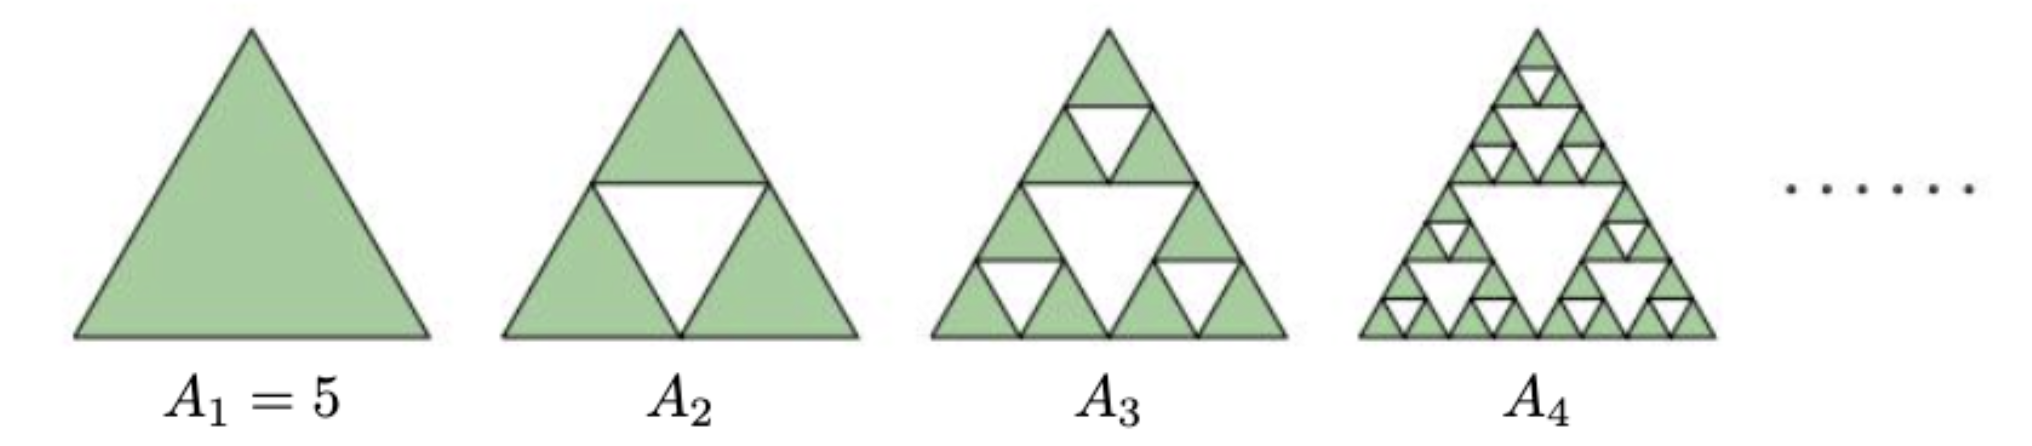
\includegraphics[width=0.8\textwidth]{media/sierpinski.png}
\end{center}

\textit{Bemerkung:} Die Figuren zeigen die ersten vier Glieder eines bekannten \textit{Fraktals}, das nach dem polnischen Mathematiker \textbf{Waclaw Franciszek Sierpinski} (1882–1969) benannt ist.

\begin{enumerate}
    \item Berechne $A_2$ und $A_3$.
    \item Bestimme die explizite Formel für $A_k$.
    \item Ab welchem $k \in \mathbb{N}$ ist $A_k$ kleiner als 0.0001?
    \item Wie viele gefärbte Dreiecke hat das $k$-te Glied bei der Konstruktion des Sierpinski-Dreiecks? Gib eine explizite Formel an.
    \item Challenge: Wie Teilaufgabe (d), jedoch sollen diesmal die weissen Dreiecke gezählt werden. \\
    \textit{Tipp:} Stelle zuerst eine rekursive Formel auf.
\end{enumerate}

        
    \end{enumerate}
\end{ueb}

\begin{ueb}
    {Programmieraufgabe}{}
    Schreiben Sie eine Python-Funktion \lstinline{isGF(liste)}, die eine Liste als Input entgegennimmt und genau dann den Wert \lstinline{True} zurückgibt, wenn die Elemente der Liste eine geometrische Folge bilden.
\end{ueb}


\clearpage
\emph{Lösungen}
\begin{enumerate}
    \item Bestimme die fehlenden Grössen dieser geometrischen Folgen (GF):
    
    \begin{center}
        \begin{tabular}{|c|c|c|c|c|c|c|}
        \hline
         & (a) & (b) & (c) & (d) & (e) & (f) \\
        \hline
        $a_1$ & 1 & 6 &  $-3$& 4 & 40 &  500\\
        \hline
        $a_n$ & 128 & 13 122 & 53 1441& 5.8564  & $-625$ & 0.16 \\
        \hline
        $n$ & 8 &  8& 12 & 5 & 4 & 6 \\
        \hline
        $q$ & 2 & 3 & $-3$ &  $1.1, -1.1$& $-2.5$ & 0.2 \\
        \hline
        $s_n$ & 255 &19 680  & 398 580 & 24.4204, 4.9724 & $-435$ & 624.96 \\
        \hline
        \end{tabular}
        \end{center}
    
    \item Anzahl der Glieder kleiner als $10^{12}$: 217
    \item Anzahl nötige Glieder:  238

    \item Berechne die Summe:
    \begin{enumerate}
        \item $\sum\limits_{k=1}^{10} \frac{5}{4}\cdot2^{k-1} = \frac{5115}{4}$
        \item $\sum\limits_{k=1}^{14} 7680 \cdot \left(\frac{1}{2}\right)^{k-1}  = 15359.0625$
        \item $\sum\limits_{k=1}^{12} -4 \cdot (-3)^{k-1}    = 531 440$
        % \item $\approx 4.42$
        % \item $\approx5173.13$
    \end{enumerate}
    
    \item Berechne die Summe:
    \begin{enumerate}
        %\item 838 861
        \item 6 560
        \item $\approx5 375 378.8$
        \item 13 107
    \end{enumerate}
    
    
    
    \item Das Sierpinski-Dreieck
    \begin{enumerate}
        \item $A_2 = 3.75$, $A_3 = 2.8125$
        \item $A_k = 5 \cdot \left( \frac{3}{4} \right)^{k-1}$
        \item $k = 39$
        \item $3^{k-1}$
        \item Die Anzahl $w_k$ der weissen Dreiecke in der $k$-te Figur ist
        $$w_k = 0 + 1 + 3 + 9 + 27 + \cdots + 3^{k-2}$$
        Mit der Formel für GR folgt $w_k = \frac{3^{k-1}-1}{2}$.
    \end{enumerate}
\end{enumerate}


















\newpage
\subsection{Die unendliche geometrische Reihe}
\subsubsection{Der Grenzwert der GR}
\begin{LA}{Einführung}{}
    Ein Baukastensatz enthält Holzwürfel. Der grösste Würfel hat eine Kantenlänge von 40 cm, die Kantenlänge des zweitgrössten misst 20 cm, die des drittgrössten 10 cm und so weiter. Ein Kind baut mit den Holzwürfeln einen Turm. Es stellt den grössten Würfel zuunterst hin, legt den zweitgrössten darauf, dann den drittgrössten und so weiter.
    \begin{enumerate}
        \item Berechnen Sie die Höhen $h_1, h_2, h_3$ und $h_{10}$ der Türme aus einem, zwei, drei und zehn Klötze.
        \item Wie viele Klötze werden benötigt, damit der Turm insgesamt einen Meter hoch wird? Wieso?
    \end{enumerate}
\end{LA}
\newpage
Die Überlegungen aus der Einführungsaufgabe lassen vermuten, dass die Glieder geometrischer Folgen $a_n = a_1 q^{n-1}$ mit $|q|<1$ für wachsende $n$ immer näher bei $0$ zu liegen kommen.
Analog wächst auch die geometrische Reihe nicht über alle Grenzen. Für wachsende $n$ nähert sich $s_n$ einer bestimmten Zahl $s$. Doch wie lässt sich $s$ aus $a_1$ und $q$ bestimmen?
Für die Summe aus $n$ Gliedern gilt:
$$s_n = a_1\cdot \frac{q^n-1}{q-1}$$
Falls nun $|q| < 1$ zum Beispiel $q=\frac{1}{2}$ ist, werden die Zahlen $q,q^2,q^3,\ldots$ immer kleiner. Die Zahl $q^{100000}$ ist dann kaum grösser als Null. Wenn $n$ gegen unendlich strebt, wird $q^n$ vernachlässigbar klein und es gilt:
$$s_n = a_1\cdot \frac{q^n-1}{q-1}   \stackrel{n\rightarrow \infty}{\longrightarrow}   s = a_1\cdot \frac{0-1}{q-1} = \frac{a_1}{1-q}$$


\begin{satz}{Unendliche geometrische Folgen und Reihen}{}
    Für die geometrische Folge
$$a_n=a_1\cdot q^{n-1}$$
gilt:
\begin{itemize}
    \item 	Falls $|q|<1$ \newline
    Die Glieder der Folge nähern sich immer mehr dem Grenzwert $0$. \newline
    Die Glieder der entsprechenden \emph{Reihe} nähern sich immer mehr dem Grenzwert
    $$ s= \frac{a_1}{1-q}$$
    \item Falls $|q|>1$ \newline
    Die Beträge der Folgenglieder wachsen über alle Grenzen. $|a_n |$ wird für wachsende $n$ unendlich gross.\newline
    Die Beträge der Reihenglieder wachsen ebenfalls über alle Grenzen. $|s_n |$ wird für wachsende $n$ unendlich gross.       
\end{itemize}
\end{satz}
\begin{definition}{Sprechweise und Notation rund um Grenzwerte}{}
Für eine geometrische Folge mit $|q|<1$ sagt man: Die Reihe \emph{konvergiert} gegen den \emph{Grenzwert} $s= \frac{a_1}{1-q}$ und man schreibt:
$$ \lim_{n \rightarrow\infty} s_n = \frac{a_1}{1-q}$$
Sprich: der \emph{Limes} für $n$ gegen unendlich von $s_n$ ist $\frac{a_1}{1-q}$

Für eine geometrische Folge mit $|q|>1$ sagt man: Die Reihe hat keinen Grenzwert. Sie \emph{divergiert}.
\end{definition}
\begin{ueb}
    {}{}

    \begin{enumerate}
        \item Ermittle den Wert der unendlichen Summe: 
        \begin{enumerate}
            \item\( 1 + \frac{1}{4} + \frac{1}{16} + \dots \)
            \item \( 5 + \frac{3}{2} + \frac{9}{20} + \dots \)
            \item \( 3 - \frac{3}{2} + \frac{3}{4} - \dots \)
           % \item \( 1 - \frac{2}{3} + \frac{4}{9} - \dots \)
            \item \( 2 + \sqrt{2} + 1 + \dots \)
            % \item \( 8 + 4\sqrt{3} + 6 + \dots \)
        \end{enumerate}
       
        \item Der Schlangenweg von $P$ nach $Q$ setzt sich aus unendlich vielen Halbkreisbögen zusammen, deren Radien eine GF mit $q = \frac{1}{2}$ bilden. Ist der Schlangenweg oder der Halbkreisweg von $P$ nach $Q$ kürzer?
        
       
        
        
        \begin{center}
            % 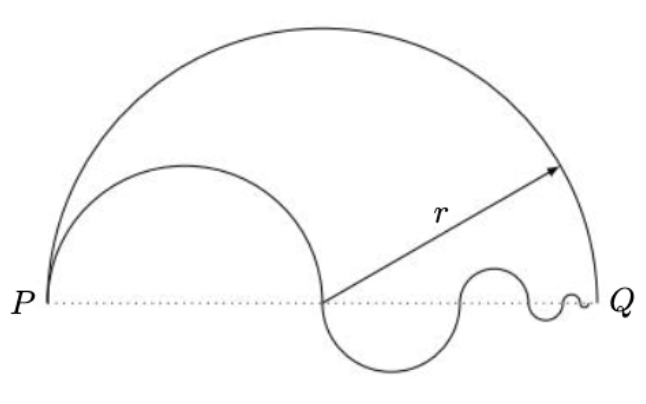
\includegraphics[width = 0.5\textwidth]{media/Schlangenweg.png}
            \begin{tikzpicture}[scale=0.3]
                % Achsen
                \draw[dotted] (-16,0) -- (16,0);
                
                % Kreise und Wellen
                \draw[blue, thick] (-16,0) arc[start angle=180, end angle=0, radius=16cm];
                \draw[red, thick] (-16,0) arc[start angle=180, end angle=0, radius=8cm];
                \draw[red, thick] (0,0) arc[start angle=180, end angle=360, radius=4cm];
                \draw[red, thick] (8,0) arc[start angle=180, end angle=0, radius=2cm];
                \draw[red, thick] (12,0) arc[start angle=180, end angle=360, radius=1cm];
                \draw[red, thick] (14,0) arc[start angle=180, end angle=0, radius=0.5cm];
                \draw[red, thick] (15,0) arc[start angle=180, end angle=360, radius=0.25cm];




                % \draw (0,0) arc[start angle=180, end angle=0, radius=2.5cm];
                % \draw (4,0) .. controls (5,-0.5) and (5.5,0.5) .. (6,0)
                %             .. controls (6.5,-0.5) and (7,0.5) .. (7.5,0)
                %             .. controls (7.75,-0.2) and (8,0.2) .. (8.2,0);
                
                % Radiuslinie
                \draw[->] (0,0) -- (45:16) node[midway, right] {$r$};
                
                % Punktebeschriftung
                \node[left] at (-16,0) {$P$};
                \node[right] at (16,0) {$Q$};
                
            \end{tikzpicture}
        \end{center}




        \item Ein Spiralförmiger Weg beginnt im Ursprung und besteht aus Strecken, deren Längen eine GF bilden. Wie lang ist der unendlich fortgesetzte Weg und wo liegt der Zielpunkt $Z$ dieses Spiralförmigen Weges?
        \begin{center}
            %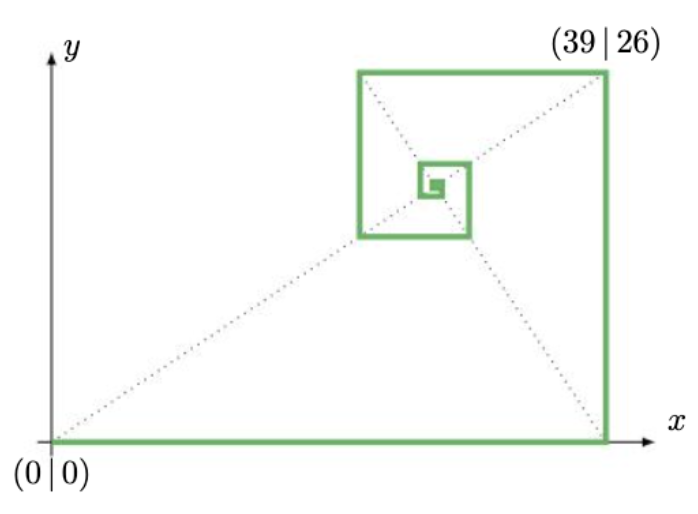
\includegraphics[width = 0.5\textwidth]{media/Spiralenweg.png}
            \begin{tikzpicture}[scale=0.5]
                % Achsen
                \draw[->] (-1,0) -- (10,0) node[right] {$x$};
                \draw[->] (0,-1) -- (0,7) node[above] {$y$};
                
                % Spiralenerstellung mit den Fibonacci-Zahlen
                \draw[thick,red] (0,0) -- (9,0) -- (9,6) -- (5,6) -- (5,10/3)
                    -- (6.77,10/3) -- (6.77,4.51) -- (5.99,4.51) -- (5.99,3.99) -- (6.33,3.99)
                     -- (6.33, 4.22);
                
                % Diagonalen
                \draw[dotted] (0,0) -- (9,6);
                \draw[dotted] (9,0) -- (5,6);
                % \draw[dotted] (8,5) -- (3,2);
                % \draw[dotted] (3,2) -- (4,2.5);
                
                % Punktebeschriftung
                \node[below left] at (0,0) {(0, 0)};
                \node[above right] at (9,6) {(39, 26)};
                
            \end{tikzpicture}
        \end{center}
        

        \item Eine unendliche geometrische Reihe beginnt mit 
        \[
        (x - 3) + \frac{1}{x - 3} + \dots \quad (x \neq 3).
        \]
        
        \begin{enumerate}
            \item Für welche Werte von \( x \) konvergiert die Reihe?
            \item Zeige, dass in diesem Fall für die Summe gilt: 
            \[
            s = \frac{(x - 3)^3}{(x - 2)(x - 4)}.
            \]
            \item Für welchen Wert von \( x \) gilt, dass \( s = x + 2 \)?
        \end{enumerate}
    \end{enumerate}
\end{ueb}

\clearpage
\emph{Lösungen}
\begin{enumerate}
    \item Ermittle den Wert der unendlichen Summe: 
    \begin{enumerate}
        \item\(  \frac{4}{3}  \)
        \item \( \frac{50}{7} \)
        \item \( 2\)
        %\item \( \frac{3}{5} \)
        \item \( 4 + 2\sqrt{2} \)
        %\item \( 32 + 16\sqrt{3} \)
    \end{enumerate}
    \item Beide Wege sind gleich lang :) .
    \item Länge 117, Endpunkt $Z=(27, 18)$
    
    \item Eine unendliche geometrische Reihe beginnt mit 
    \(
    (x - 3) + \frac{1}{x - 3} + \dots \quad (x \neq 3).
    \)
    
    \begin{enumerate}
        \item $x<4$ oder $x<2$.
        \item \dots
        \item \( x \approx 4.10\)
    \end{enumerate}
\end{enumerate}




























\newpage
\subsubsection{Dezimalbruchdarstellung rationaler und irrationaler Zahlen}
Bereits in der ersten Klasse haben Sie gelernt, dass Zahlen mit einer unendlichen, periodischen Dezimaldarstellung einem gewöhnlichen Bruch entsprechen. Allerdings konnten wir es damals nicht begründen. Heute werden Sie sehen, dass konvergente unendliche geometrische Reihen der Schlüssel für die Umwandlung solcher Zahlen in Brüche sind. Betrachten Sie dazu folgende Beispiele:
\begin{bsp}{Umwandlung von periodischen Zahlen in Brüche}{}
    \vspace*{15cm}
%    \begin{itemize}
%     \item Mit Periode, die aus einer Ziffer besteht:
%     \begin{align*} 0.\overline{4} 
%         &= 0.4444\cdots = 0.4 + 0.04 + 0.004 + \cdots = \frac{4}{10} + \frac{4}{100} +\frac{4}{1000} +\cdots = \\
%                                     &= \frac{4}{10} \left( 1+\frac{1}{10} + \frac{1}{100} + \cdots \right) = \frac{4}{10}\cdot \frac{1}{1-\frac{1}{10}}=\frac{4}{9}
%         \end{align*}

%     \item  Mit Periode, die aus zwei Ziffern besteht:
%     \begin{align*} 0.\overline{37} &= 0.373737\cdots = 0.37 + 0.0037 + 0.000037 + \cdots = \frac{37}{100} + \frac{37}{10000} +\frac{37}{1000000} +\cdots = \\
%                                     &= \frac{37}{100} \left( 1+\frac{1}{100} + \frac{1}{10000} + \cdots \right) = \frac{37}{100}\cdot \frac{1}{1-\frac{1}{100}}=\frac{37}{99}
%         \end{align*}
%     \item  Wenn die Periode nicht gleich nach dem Dezimalpunkt steht:
%         \begin{align*} 0.135\overline{37} = \frac{135}{1000} + \frac{37}{10^5}\left( 1+\frac{1}{100} + \frac{1}{10000} + \cdots \right) = \frac{135}{1000} + \frac{37}{10^5} \cdot \frac{1}{1-\frac{1}{100}}=\frac{6701}{49500}
%             \end{align*} 
%     \end{itemize}
\end{bsp}

\clearpage

\begin{ueb}
    {}{}
    \begin{enumerate}
        % \item Verwandeln Sie die folgenden Zahlen in Brüche
        % \begin{tasks}(3)
        %     \task $0.\overline{7}$
        %     \task $0.\overline{54}$
        %     \task $0.\overline{612}$
        %     \task $2.\overline{04}$
        %     \task $0.63\overline{123}$
        %     \task $1.00\overline{35}$
        % \end{tasks}
        \item  Verwandle den periodischen Dezimalbruch in einen gewöhnlichen Bruch. (Überprüfen Sie das Resultat mit dem Taschenrechner)

        \begin{enumerate}
            %\item \( 0.\overline{5} \)
            %\item \( 0.\overline{54} \)
            \item \( 0.\overline{543} \)
            %\item \( 0.1\overline{3} \)
            \item \( 0.25\overline{7} \)
            \item \( 0.4\overline{81} \)
        \end{enumerate}
        
        \item Aus den Überlegungen oben folgt, dass jede Zahl mit einer endlichen oder periodischen Dezimaldarstellung einem Bruch entspricht. Es gilt auch die \emph{Umkehrung}: Die Dezimaldarstellung eines Bruchs ist immer endlich oder periodisch. Die folgenden Aufgaben sollen Ihnen helfen zu verstehen, wieso das so ist.
        \begin{enumerate}
            \item Finden Sie die Dezimaldarstellung von $\frac{1}{7}$, indem Sie schriftlich dividieren:
            \begin{align*}
                &1.00000 : 7 = 0.1\ldots \\
                &10 \\
                &\phantom{1}30
            \end{align*}
            \item 	Wann beginnt sich die Dezimaldarstellung zu wiederholen? Wie viele verschiedene Reste kann es bei einer Division durch eine ganze Zahl $n$ geben?
            \item 	Wieso ist die Dezimaldarstellung von $\frac{1}{n}$ endlich oder periodisch? Wie lang kann die Periode sein?
        \end{enumerate}
        
    \end{enumerate}
\end{ueb}

% \emph{Lösungen}
% \begin{enumerate}

%     \item  Verwandle den periodischen Dezimalbruch in einen gewöhnlichen Bruch.

%     \begin{enumerate}
%         %\item \( \frac{5}{9}  \)
%         %\item \( \frac{6}{11} \)
%         \item \( \frac{181}{333}  \)
%         %\item \(\frac{2}{15}  \)
%         \item \( \frac{58}{225}  \)
%         \item \( \frac{53}{110}  \)
%     \end{enumerate}
    
%     \item \dots 
%     \end{enumerate}


\newpage
\section{Grenzwerte}
\subsection{Grenzwerte von Folgen}
Bis jetzt haben wir den Begriff des Grenzwertes nur für das Beispiel der geometrischen Folgen und Reihen verwendet. In diesem Kapitel möchten wir uns der Frage stellen, ob auch andere Arten von Folgen konvergieren. Dazu benötigen wir erstmals eine präzise Definition des Grenzwertbegriffs.
\subsubsection{Definition des Grenzwertes}
Etwas naiv formuliert, könnte man sagen: \glqq Der Grenzwert einer Folge ist jene Zahl, an die sich die Folgenglieder immer mehr nähern\grqq{}. Wenn man es sich genau überlegt, merkt man aber, dass diese naive Sichtweise nicht ausreicht. Betrachten Sie dazu folgende Beispiele:

\emph{Wieso ist der Grenzwert nicht 100?}

% \begin{tikzpicture}
%     % Achsen
%     \draw[->] (0,0) -- (12,0) node[right] {$n$};
%     \draw[->] (0,0) -- (0,12) node[above] {$h$};

%     % Raster
%     \draw[gray, thin] (0,0) grid (11,11);

%     % Punkte
%     \foreach \x/\y in {1/40, 2/60, 3/70, 4/75, 5/77.5, 6/78.75, 7/79.375, 8/79.6875, 9/79.92, 10/79.96, 11/79.98} {
%         \fill[red] (\x, \y/10) circle (0.15);
%     }

%     % Achsenbeschriftung
%     \node[left] at (0,10) {100};
%     \node[below] at (10,0) {20};

% \end{tikzpicture}




 
\begin{figure}[htbp]
	\begin{minipage}{0.5\textwidth}
		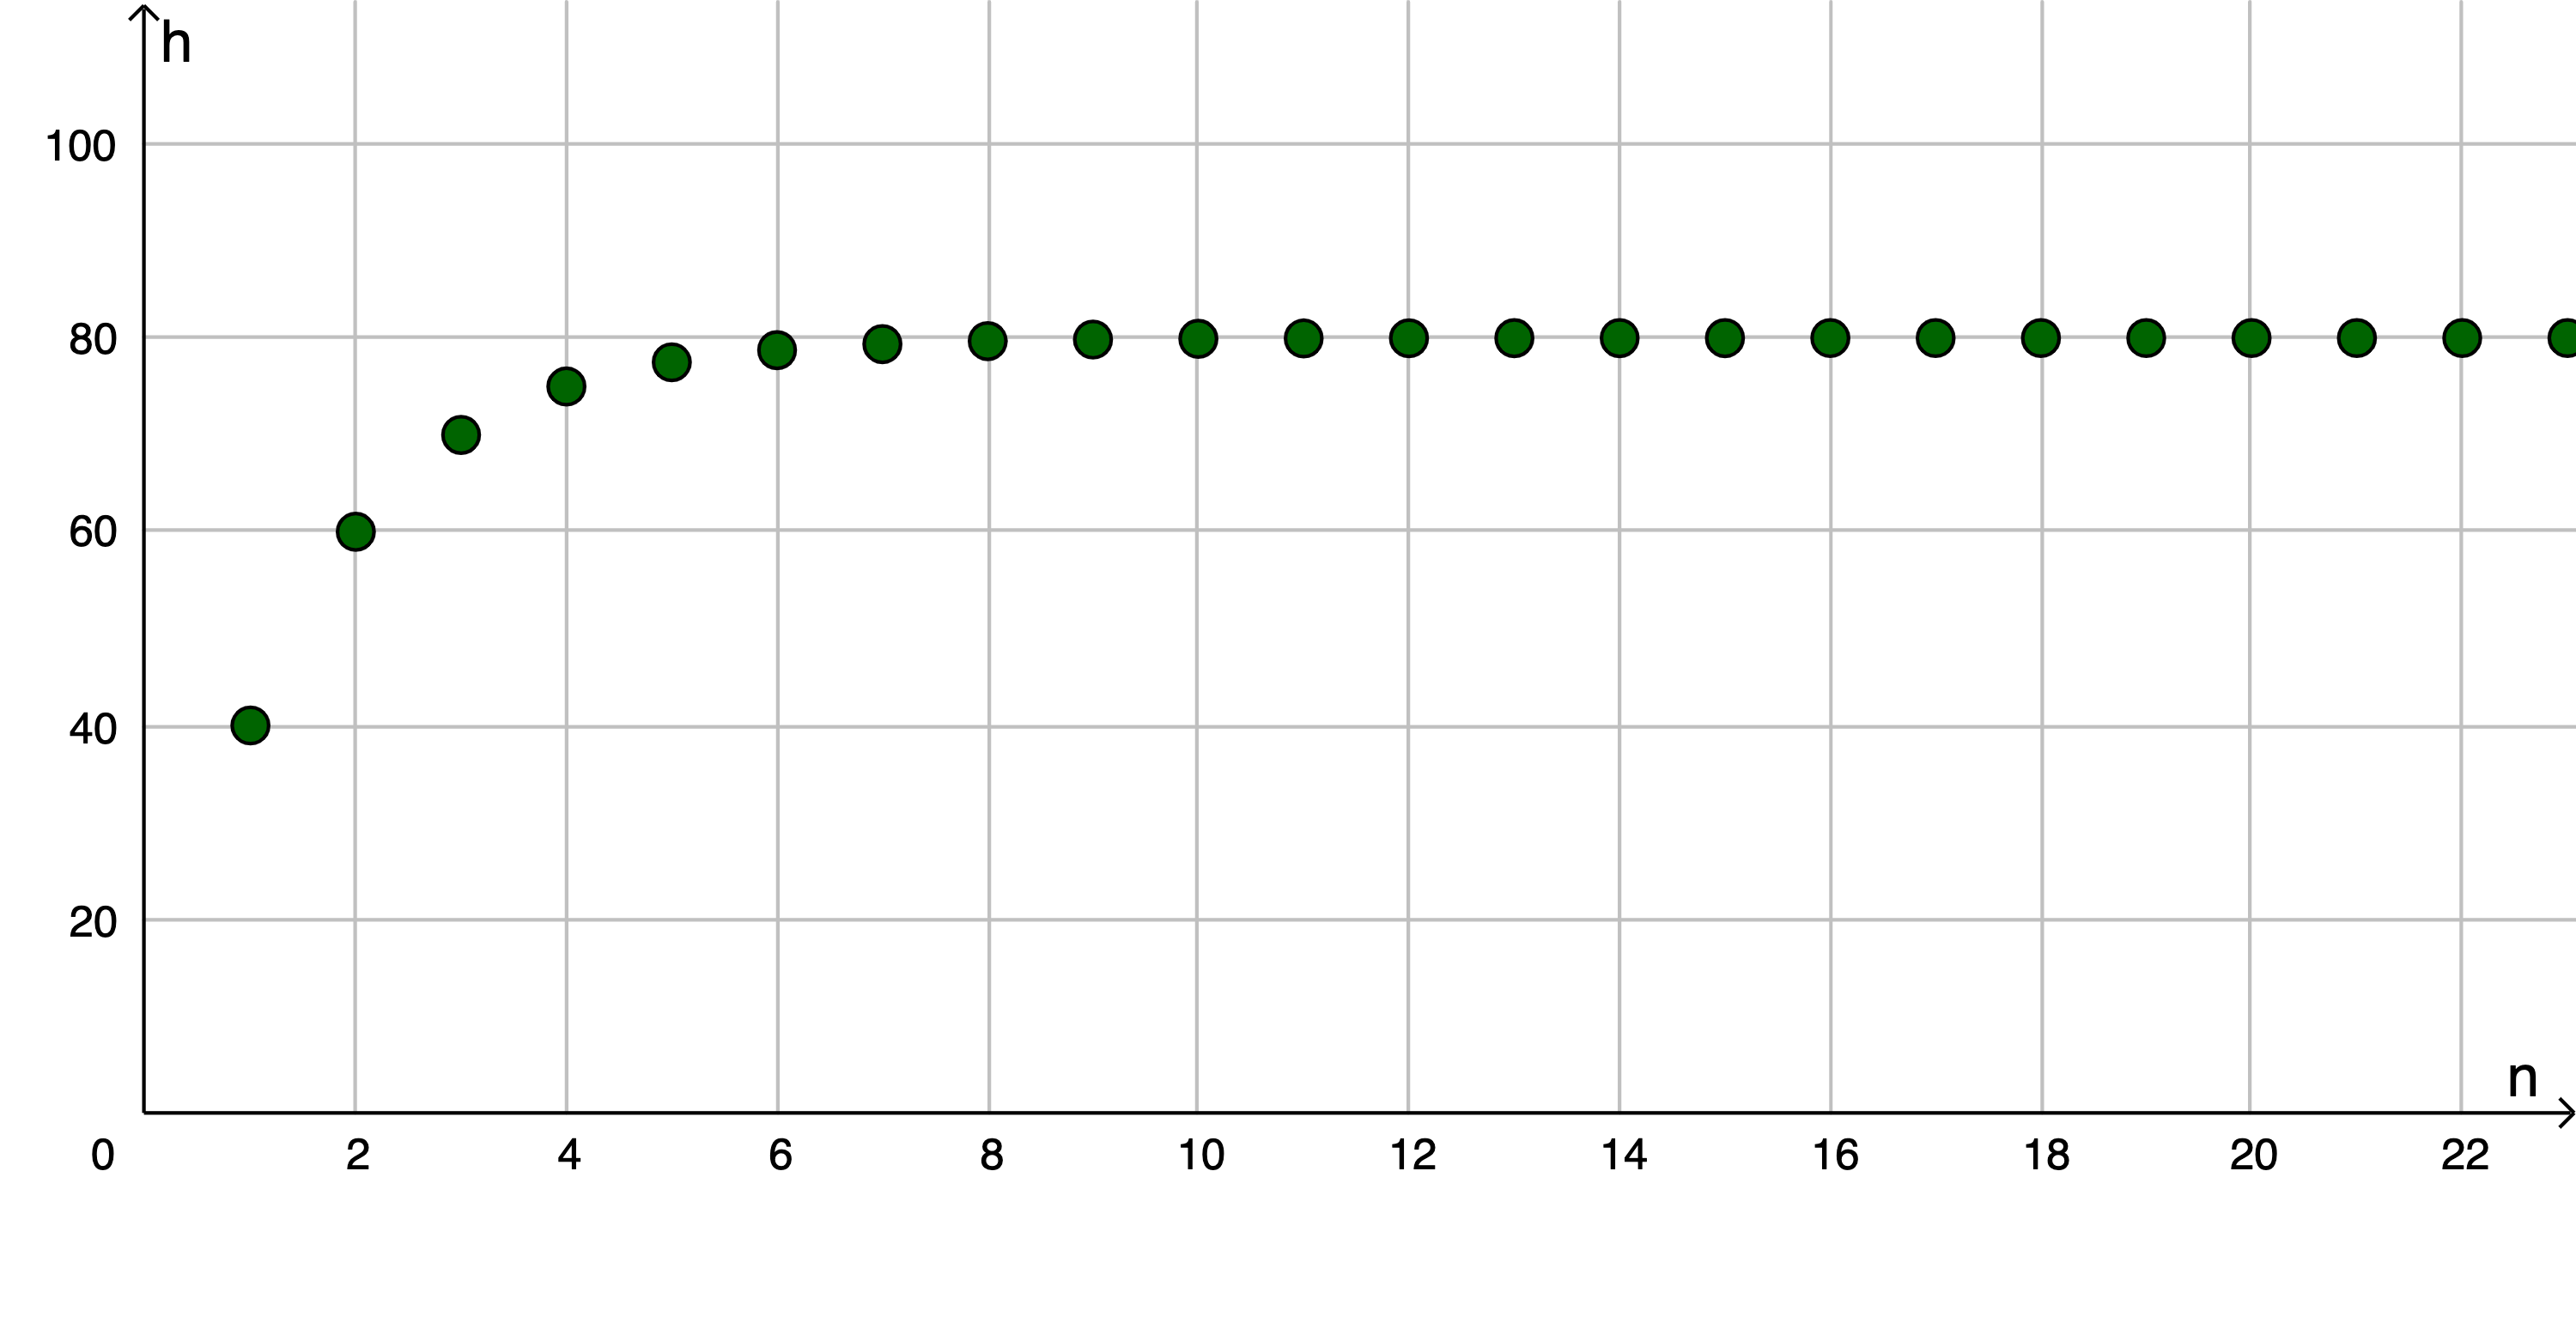
\includegraphics[width=\textwidth]{media/HoeheDerTuerme.png}
	\end{minipage}
	\hfill
	\begin{minipage}{0.3\textwidth}

	\end{minipage}
\end{figure}


% 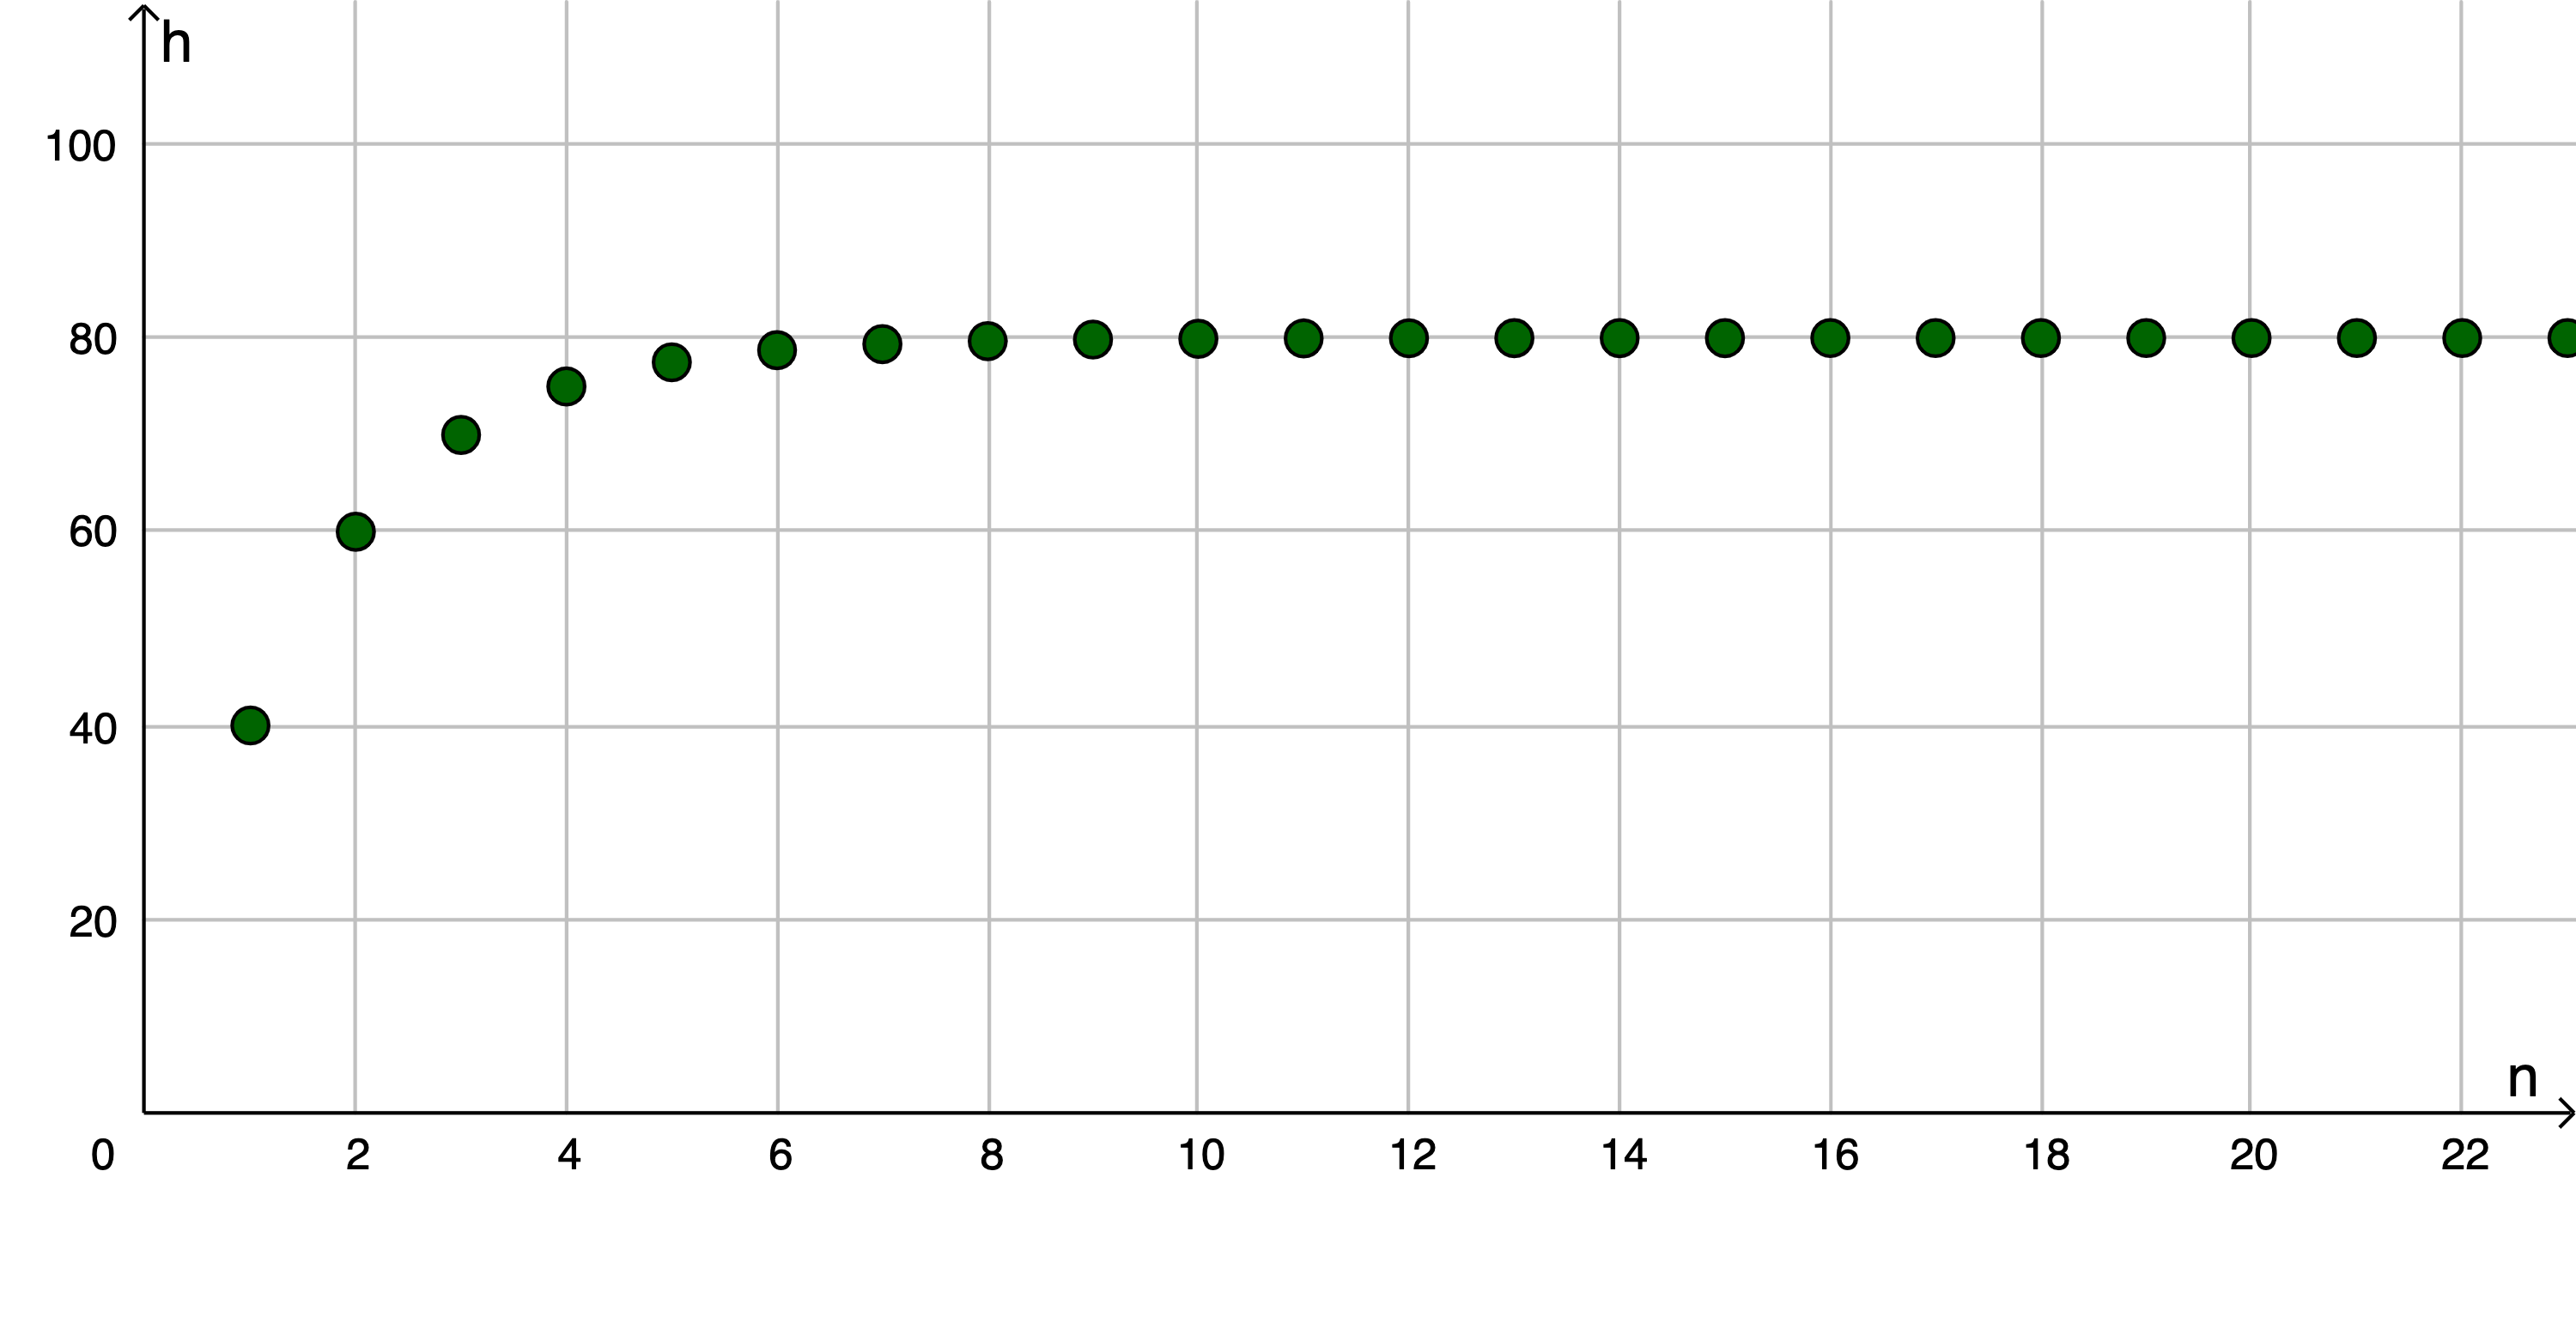
\includegraphics[scale=0.5]{media/HoeheDerTuerme.png} \newline
% \emph{Wieso ist der Grenzwert nicht 100?}
%Die Folgenglieder nähern zwar auch der Zahl 100 immer mehr, aber der Abstand zwischen Folgenglied und 100 ist immer grösser als 20. Erkenntnis: Jeder noch so kleine Abstand zwischen Folgenglieder und vermeintlichen Grenzwert muss unterschritten werden!
%\clearpage
\emph{Wieso ist der Grenzwert nicht 80?}
\begin{figure}[htbp]
	\begin{minipage}{0.5\textwidth}
		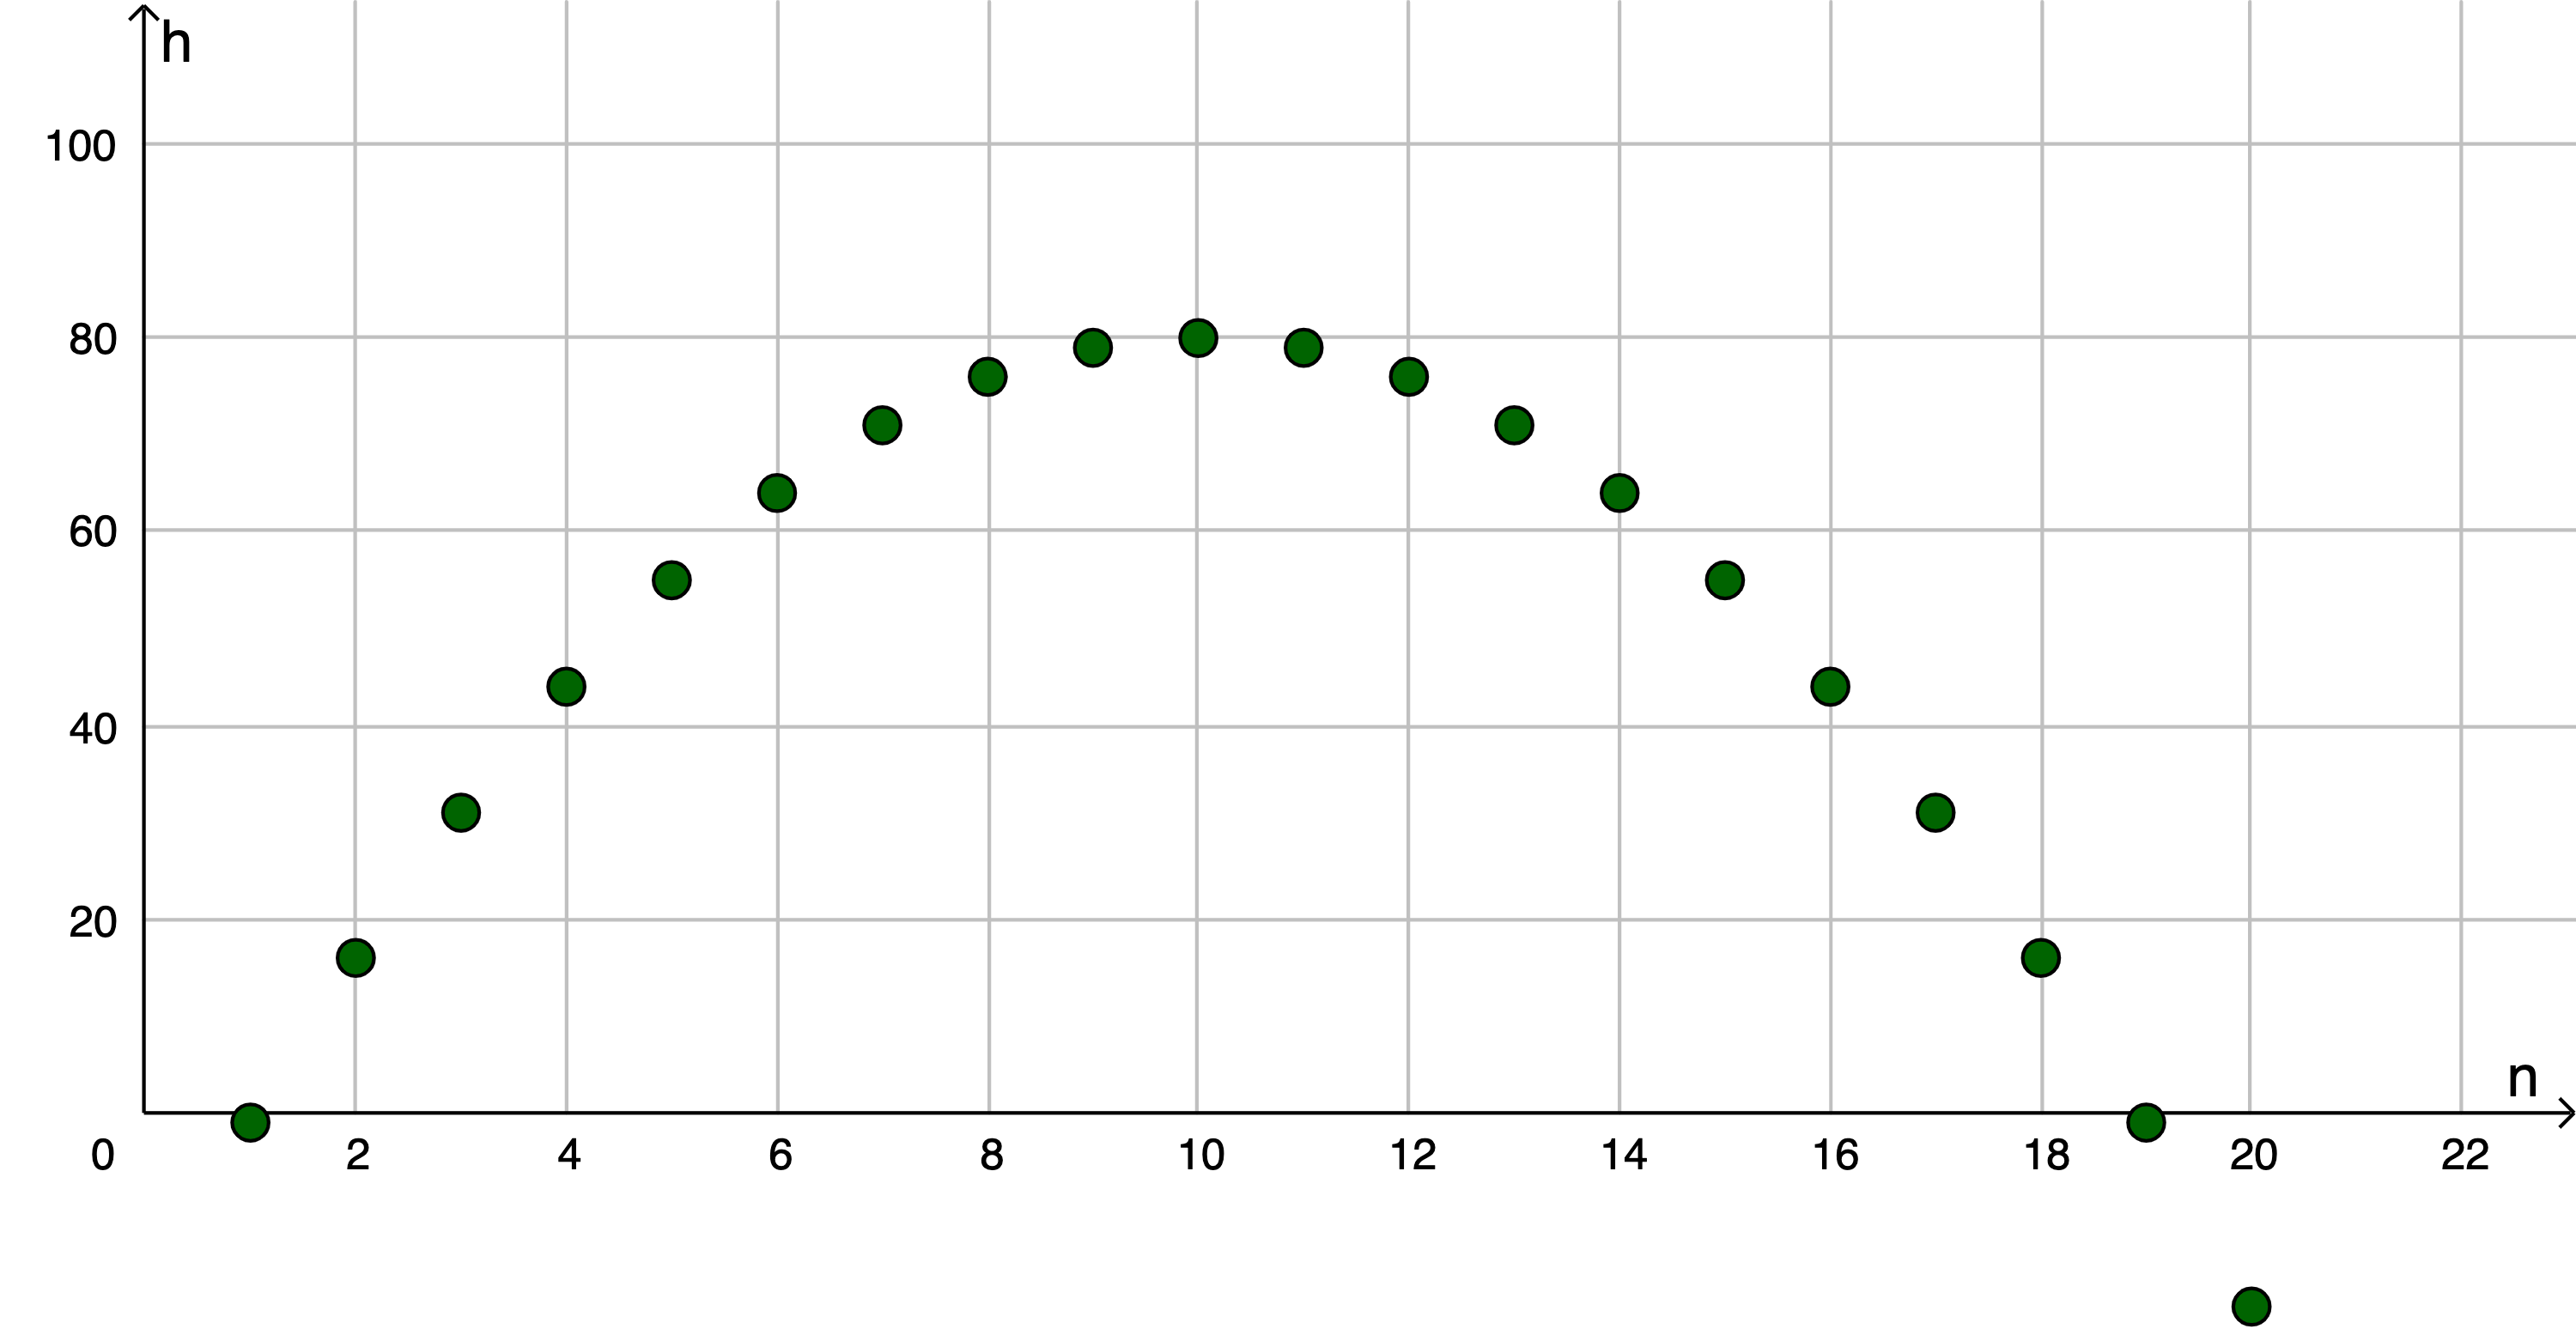
\includegraphics[width=\textwidth]{media/WiesoNicht80.png}
	\end{minipage}
	\hfill
	\begin{minipage}{0.3\textwidth}

	\end{minipage}
\end{figure}
% 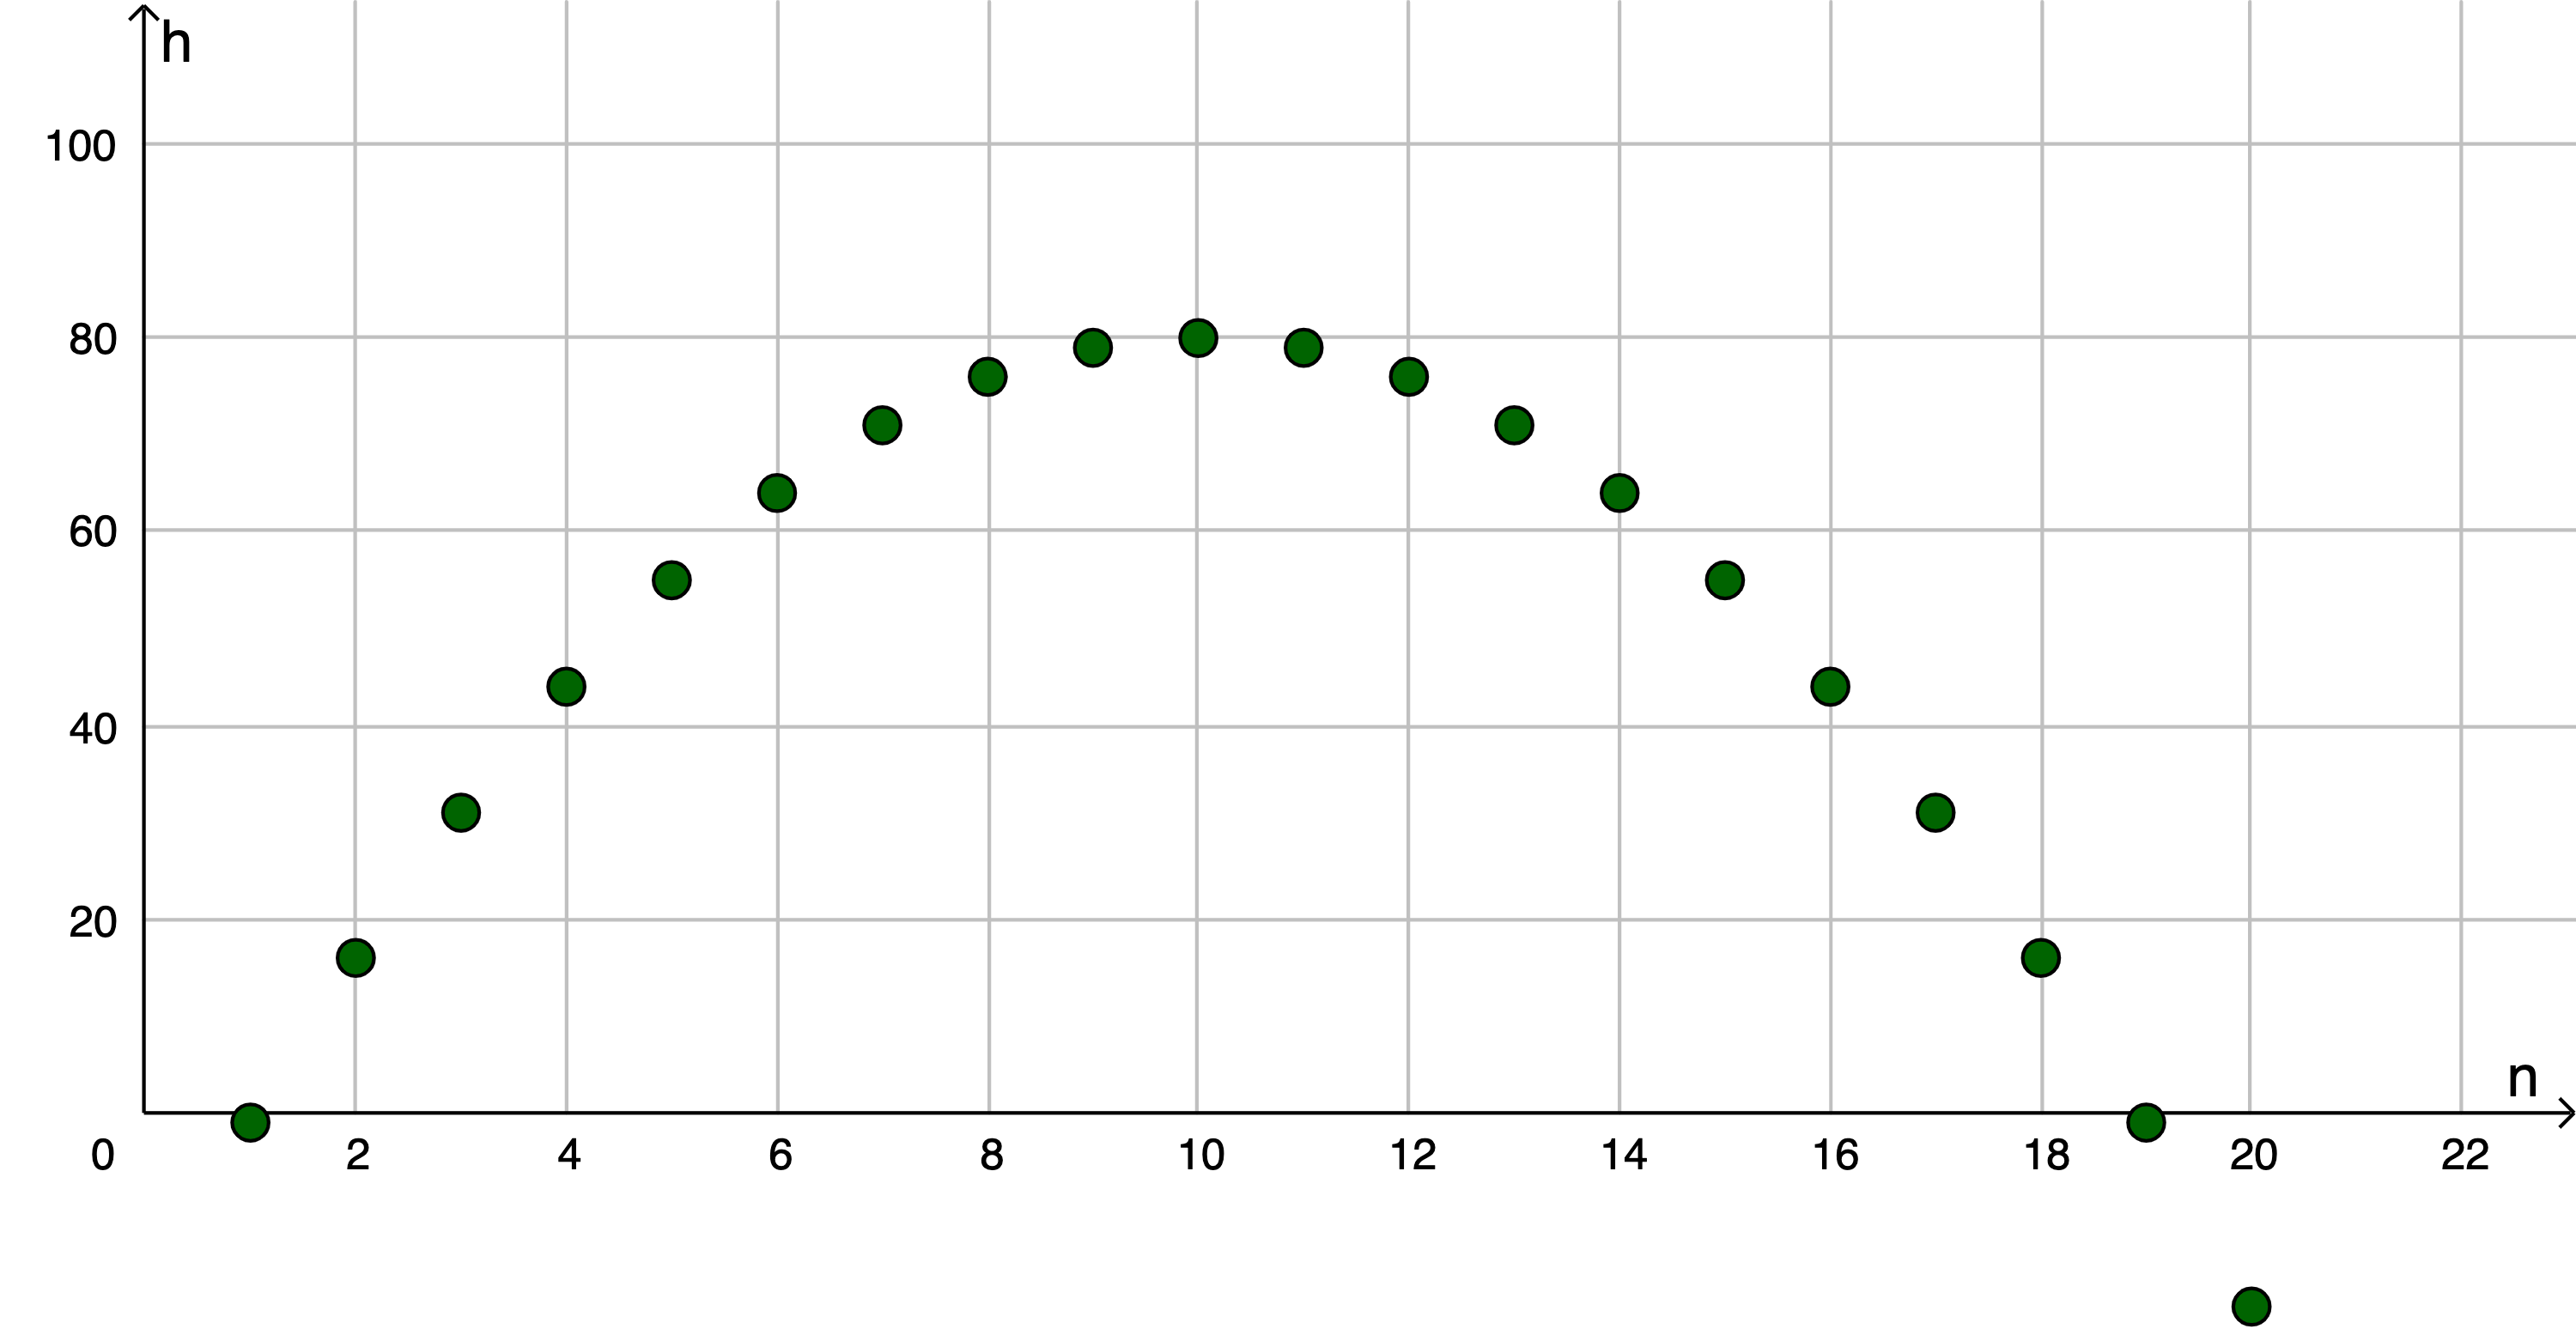
\includegraphics[scale=0.5]{media/WiesoNicht80.png}\newline
% \emph{Wieso ist der Grenzwert nicht 80?}
%Das 10. Glied der Folge im Bild oben ist tatsächlich genau 80. Aber die weiteren Folgenglieder entfernen sich wieder von 80. Erkenntnis: Der Abstand zwischen Folgenglieder und vermeintlichem Grenzwert darf nicht wieder grösser werden!
\clearpage
\begin{definition}{Grenzwert einer Folge}{}
	Eine Zahl $g$ heisst Grenzwert der Folge $a_n$, falls es für jeden noch so kleinen Abstand $\varepsilon>0$ einen Schwellwert $N$ gibt, sodass ab dem $N$-ten Glied der Folge alle Glieder sich um weniger als $\varepsilon$ von $g$ unterscheiden.\newline
	In der Mathematik wird das häufig so angegeben: \newline
	Eine Zahl $g$ heisst Grenzwert der Folge $a_n$, falls: Für alle $\varepsilon>0$ ein $N \in \N$ existiert, sodass für alle $n>N$ gilt
	$$ |a_n - g| < \varepsilon $$
\end{definition}
Anders gesagt: Für jedes (noch so kleine) $\varepsilon > 0$ gibt es eine Schwelle, ab welcher sich alle Folgenglieder in einem \glqq $\varepsilon$-Band\grqq{} um den Grenzwert befinden - also im Bereich Grenzwert$\pm \varepsilon$.

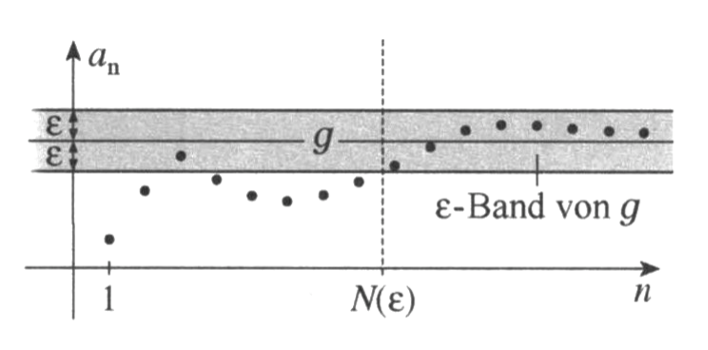
\includegraphics{media/epsilonband.png}

Sprech- und Schreibweisen rund um den Grenzwert:
\begin{itemize}
	\item \glqq Die Folge $a_n$ \emph{konvergiert}\grqq{}.
	\item \glqq Die Folge $a_n$ \emph{strebt} gegen den Grenzwert $g$\grqq{}.
	\item $\lim\limits_{n\rightarrow\infty} a_n = g$ \glqq Der Limes der Folge $a_n$ für $n$ gegen unendlich ist $g$\grqq{}.
	\item $a_n \rightarrow g$ für $n\rightarrow \infty$.
\end{itemize}

Nicht alle Folgen haben einen Grenzwert. Zwei Beispiele für Folgen, die nicht konvergieren:

\begin{figure}[htbp]
	\begin{minipage}{0.5\textwidth}
		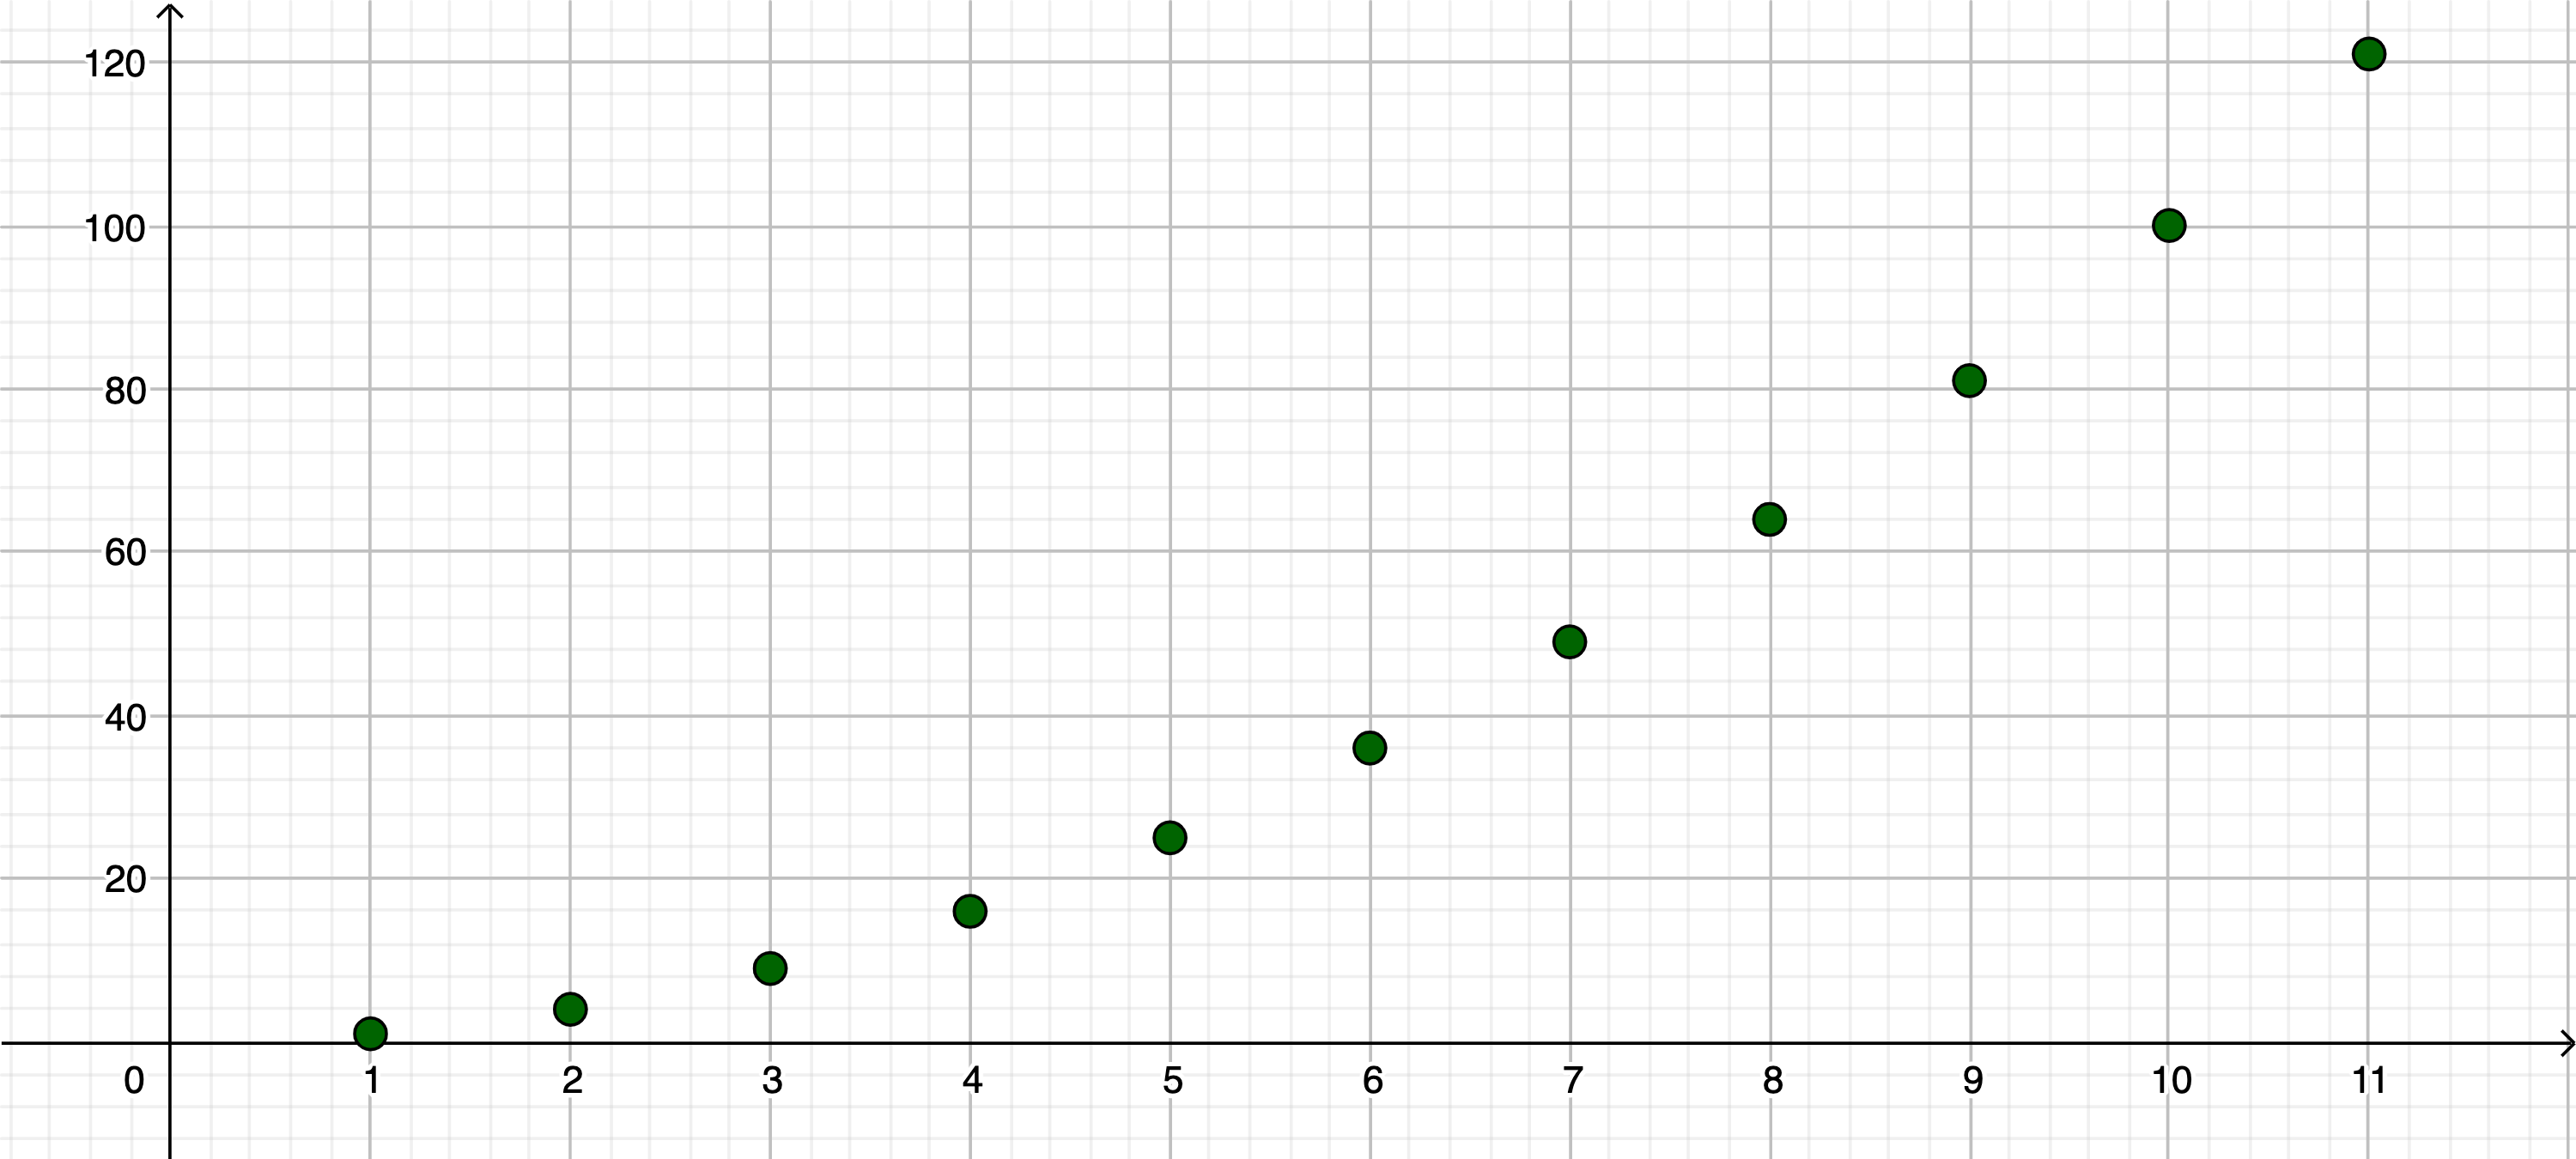
\includegraphics[width=\textwidth]{media/folgeQuadratzahlen.png}
	\end{minipage}
	\hfill
	\begin{minipage}{0.4\textwidth}
		Das Bild zeigt die Folge der Quadratzahlen. Die Glieder dieser Folge wachsen über alle Grenzen. Man sagt: \glqq Die Folge ist divergent\grqq{}. Weil in diesem Fall die Glieder \glqq unendlich gross werden\grqq{}, sagt man auch \glqq die Folge hat den uneigentlichen Grenzwert $\infty$\grqq{} und schreibt $\lim\limits_{n\rightarrow\infty} a_n = \infty$
	\end{minipage}
\end{figure}

\begin{figure}[ht]
	\begin{minipage}{0.5\textwidth}
		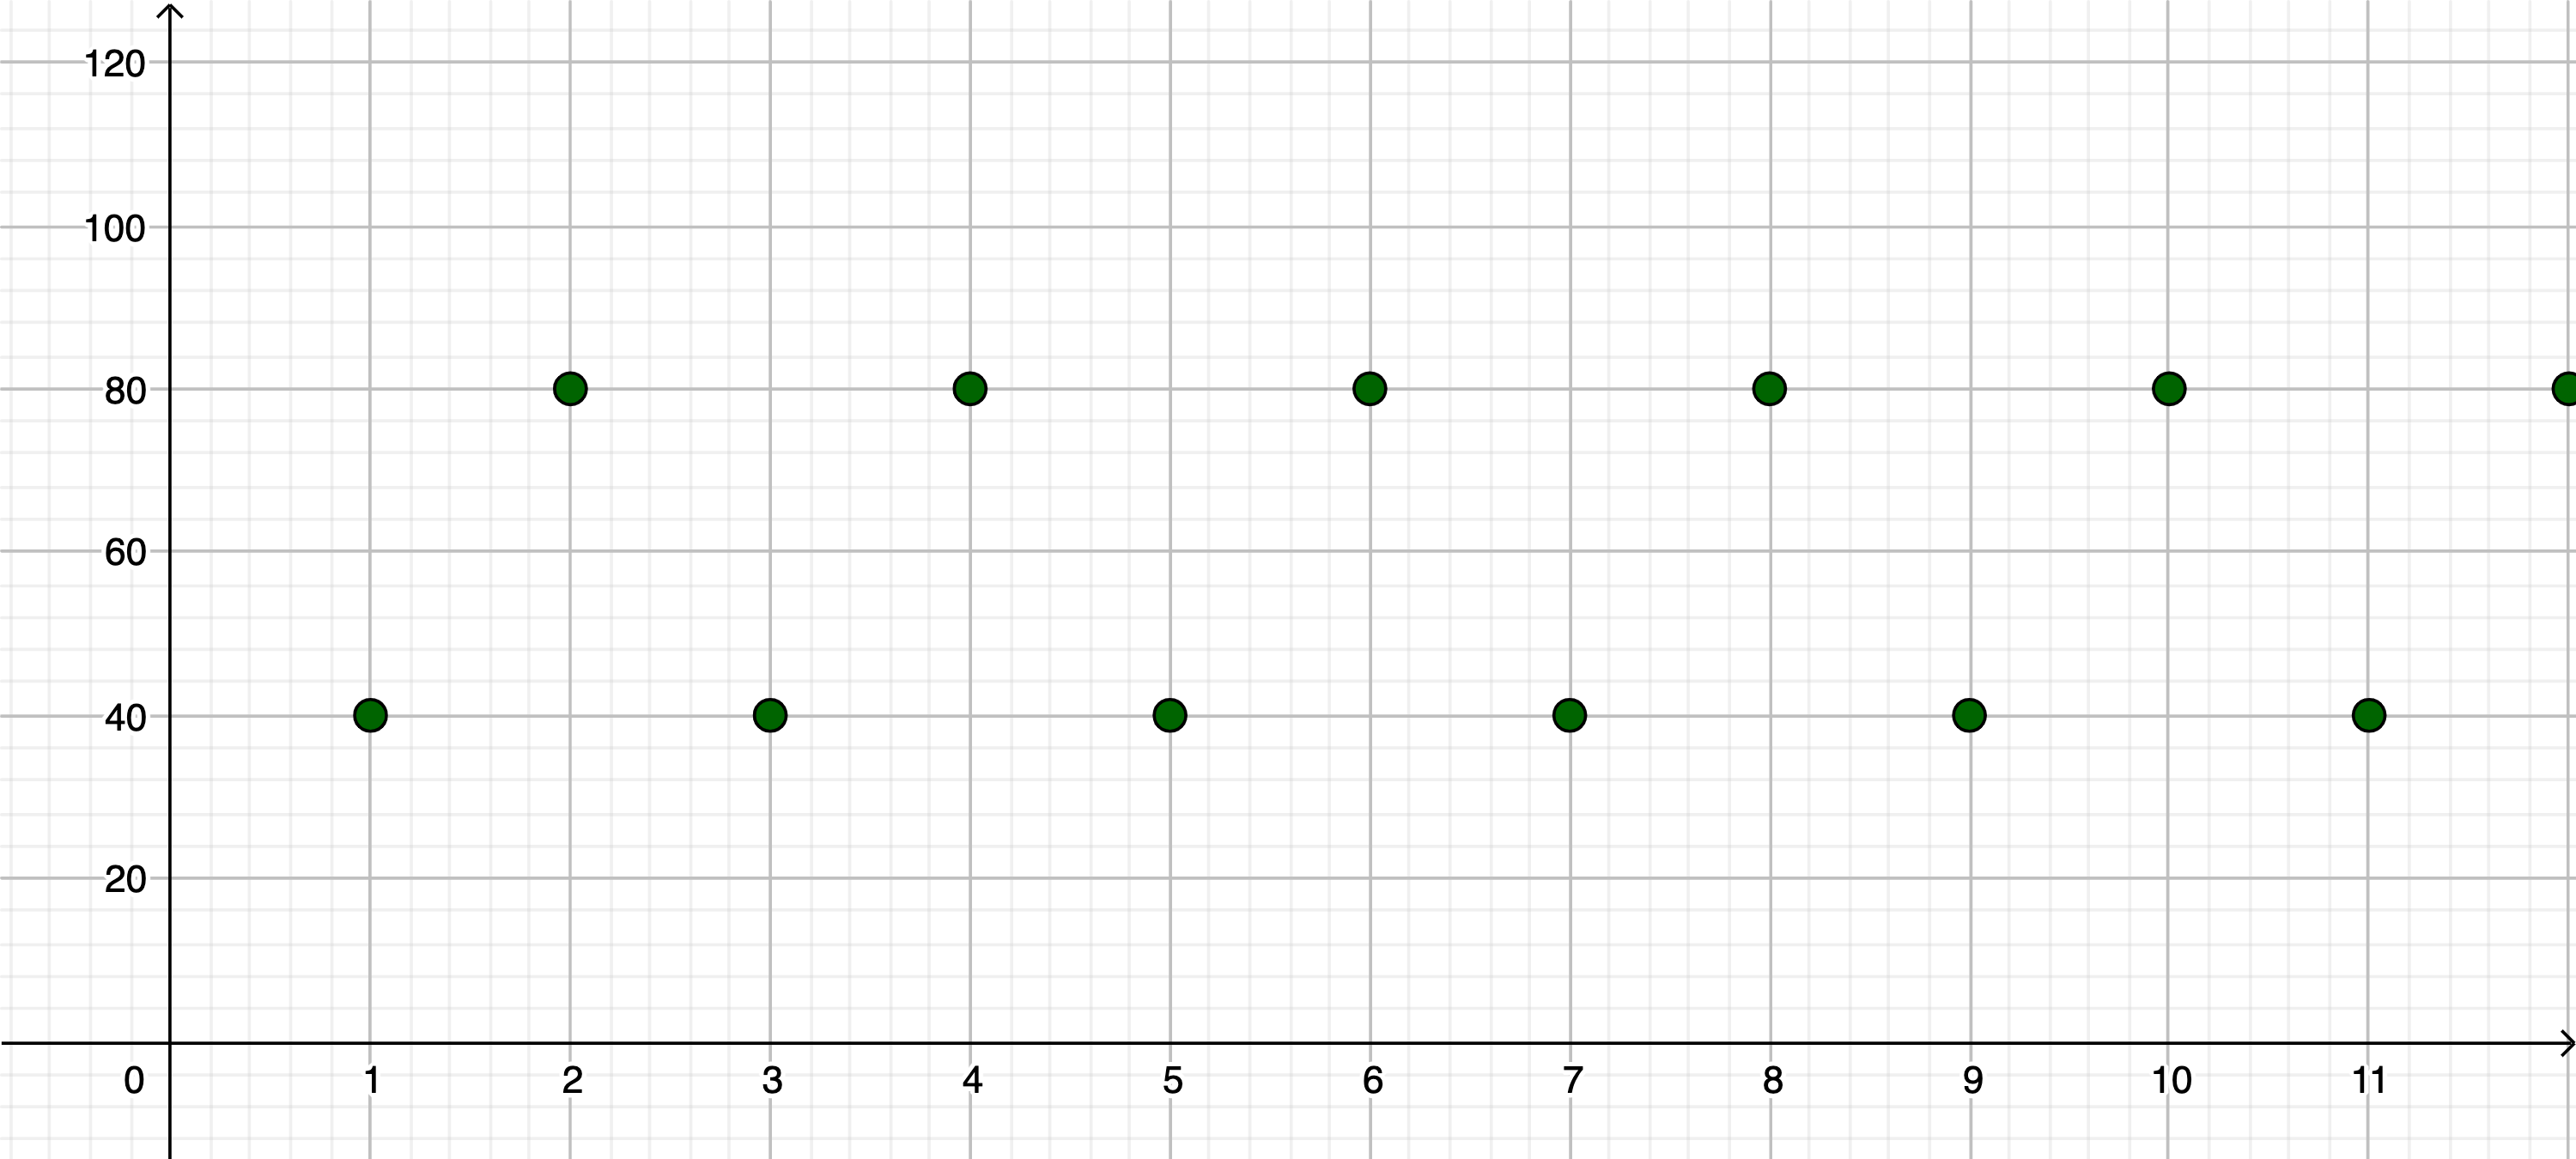
\includegraphics[width=\textwidth]{media/folgeAlternierend.png}
	\end{minipage}
	\hfill
	\begin{minipage}{0.4\textwidth}
		Die Folge in diesem Bild wächst zwar nicht über alle Grenzen, hat aber auch keinen Grenzwert. Sie ist divergent. Der $\lim\limits_{n\rightarrow\infty} a_n$ existiert nicht.
	\end{minipage}
\end{figure}



\begin{bsp}[unbreakable]{Untersuchung der Folge $a_n=\frac{2}{n^2}$}{}

	%\vspace*{16cm}
	Die ersten Glieder der Folge $a_n=\frac{2}{n^2}$ sind: $2, 0.5, 0.2\bar{2}, 0.125, 0.08, 0.05\bar{5}, ...$.
	\bigskip

	\emph{Behauptung}: Die Folge $a_n=\frac{2}{n^2}$  strebt gegen den Grenzwert Null.
	\begin{proof}
		Sei $\varepsilon>0$ eine beliebige (noch so kleine) positive Zahl. Sei dann $N=\sqrt{\frac{2}{\varepsilon}}$ . Nun gilt für alle $n>N$:
		$$ |a_n-0|=|a_n | = \left| \frac{2}{n^2} \right| < \left| \frac{2}{N^2} \right| = \left| \frac{2}{\frac{2}{\varepsilon}} \right| = |\varepsilon| = \varepsilon$$

	\end{proof}
\end{bsp}

Genau gleich kann man allgemein zeigen:
\begin{satz}{Nullfolgen}{}
	Sei $a_n =\frac{c}{n^k}$  mit $k>0$ und $c\in \R$. Dann gilt:
	$$\lim_{n \rightarrow \infty} a_n = 0$$
\end{satz}
\clearpage
\begin{bsp}
	{Schwelle zu gegebener $\varepsilon$-Umgebung bestimmen}{}
	Gegeben ist die Folge $a_n = \frac{2n}{n+1}$. Der Grenzwert der Folge ist $g=2$. Laut Definition gibt es für alle $\varepsilon>0$ eine Zahl $N\in \N$, sodass für alle $n>N$:  $|a_n-g|<\varepsilon$ ist. Bestimmen Sie die kleinstmögliche Zahl $N$ für $\varepsilon= \frac{1}{100}$.
	\vspace*{14cm}
\end{bsp}
\clearpage
\begin{ueb}{}{}
	\begin{enumerate}
		\item
		      Untersuchen Sie die Folge $n \mapsto a_n$. Was vermuten Sie: Ist sie konvergent oder divergent? Was ist der vermutete Grenzwert bzw. die Art der Divergenz an.

		      \begin{enumerate}
			      \item $a_n = \frac{2}{n+2}$
			      \item $a_n = \frac{2n}{n+2}$
			      \item $a_n = \frac{2^n}{n+2}$
			      \item $a_n = \frac{2n + (-1)^n}{n}$
			      \item $a_n = \frac{2 + n \cdot (-1)^n}{n}$
			      \item $a_n = 3 - n \cdot (-1)^n$
			      \item $a_n = \left(1 - \frac{1}{n}\right)^4$
			      \item $a_n = \left(1 - \frac{1}{4}\right)^n$
			      \item $a_n = 2^{-1/n}$
			      \item $a_n = \cos(n\cdot \pi)$
			      \item $a_n = \sin(n\cdot \pi)$
		      \end{enumerate}



		\item Bestimme den Grenzwert $g$ der Folge. Von welchem $n$ an liegen alle Glieder innerhalb der gegebenen $\varepsilon$-Umgebung von $g$?

		      \begin{enumerate}
			      \item $a_n = \frac{1}{2n - 5}, \quad \varepsilon = 0.1$
			            %\item $a_n = \frac{50}{n^2}, \quad \varepsilon = 0.05$
			      \item $a_n = \frac{n - 1}{n + 5}, \quad \varepsilon = 0.02$
			            %\item $a_n = \frac{3n}{n + 4}, \quad \varepsilon = 0.01$
			      \item $a_n = \frac{8}{2^{n-2}}, \quad \varepsilon = 0.0001$
			            %\item $a_n = \frac{2 - 3n^2}{n^2}, \quad \varepsilon = 0.001$
		      \end{enumerate}
	\end{enumerate}
\end{ueb}

\clearpage
\emph{Lösungen}
\begin{enumerate}
	\item \begin{enumerate}
		      \item $a_n = \frac{2}{n+2}$, \quad Grenzwert: $0$
		      \item $a_n = \frac{2n}{n+2}$, \quad Grenzwert: $2$
		      \item $a_n = \frac{2^n}{n+2}$, \quad divergiert gegen $\infty$
		      \item $a_n = \frac{2n + (-1)^n}{n}$, \quad Grenzwert: $2$
		      \item $a_n = \frac{2 + n \cdot (-1)^n}{n}$, \quad unbestimmt divergent
		      \item $a_n = 3 - n \cdot (-1)^n$, \quad unbestimmt divergent ($\pm \infty$)
		      \item $a_n = \left(1 - \frac{1}{n}\right)^4$, \quad Grenzwert: $1$
		      \item $a_n = \left(1 - \frac{1}{4}\right)^n$, \quad Grenzwert: $0$
		      \item $a_n = 2^{-1/n}$, \quad Grenzwert: $1$
		      \item $a_n = \cos(n\cdot \pi)$, \quad unbestimmt divergent
		      \item $a_n = \sin(n\cdot \pi)$, \quad Grenzwert: $0$
	      \end{enumerate}

	\item
	      \begin{enumerate}
		      \item $a_n = \frac{1}{2n - 5}, \quad \varepsilon = 0.1$, \quad Grenzwert: $0$, ab $n \geq 8$
		            %\item $a_n = \frac{50}{n^2}, \quad \varepsilon = 0.05$, \quad Grenzwert: $0$, ab $n \geq 32$
		      \item $a_n = \frac{n - 1}{n + 5}, \quad \varepsilon = 0.02$, \quad Grenzwert: $1$, ab $n \geq 296$
		            %\item $a_n = \frac{3n}{n + 4}, \quad \varepsilon = 0.01$, \quad Grenzwert: $3$, ab $n \geq 1197$
		      \item $a_n = \frac{8}{2^{n-2}}, \quad \varepsilon = 0.0001$, \quad Grenzwert: $0$, ab $n \geq 19$
		            %\item $a_n = \frac{2 - 3n^2}{n^2}, \quad \varepsilon = 0.001$, \quad Grenzwert: $-3$, ab $n \geq 45$
	      \end{enumerate}



\end{enumerate}


























\newpage
\subsubsection{Die Grenzwertsätze}
Das Bestimmen des Grenzwertes und der Nachweis der Konvergenz mit der Definition kann ziemlich aufwendig sein. Einfacher geht es mit den sogenannten Grenzwertsätzen:
\begin{LA}{Einführungsaufgabe}{}
	Betrachten Sie die Folge $a_n=\frac{9n^2+4}{3n^2}$
	\begin{enumerate}
		\item Berechnen Sie $a_1,a_5$ und $a_{10}$.
		\item Welchen Grenzwert hat die Folge vermutlich?
	\end{enumerate}
	Wenn man sehr grosse Zahlen für $n$ einsetzt, kann man leicht eine Vermutung für den Grenzwert der Folge aufstellen. Allerdings kann man nicht ausschliessen, dass man für wirklich sehr grosse $n$ (z.B. $n=10^{{10^9}}$) ganz andere Zahlen erhalten würde; nicht zuletzt deshalb, weil es keinen Computer gibt, der zuverlässig mit solch grossen Zahlen rechnen kann – und es gibt noch viel, viel grössere Zahlen! Durch geschicktes Umformen der Definition der Folge können wir unsere Vermutung aber begründen:
	\begin{enumerate}
		\item Die Definition der Folge $a_n$ kann auch so umgeformt werden:
		      $$a_n=\frac{9n^2}{3n^2}+\frac{4}{3n^2}=3 + \frac{4}{3n^2}$$
		      Was passiert mit den Summanden in der Definition der Folge, wenn $n$ immer grösser wird? Was bedeutet das für den Grenzwert?
		\item Bestimmen Sie den Grenzwert der Folge $b_n=\frac{2n+10}{5n}$, indem Sie den Term zuerst umformen.
		\item Wie lautet der Grenzwert der Folge $c_n= \frac{9n^2+4}{3n^2} + \frac{2n+10}{5n}$?
	\end{enumerate}
\end{LA}
\newpage
In den Einführungsaufgaben haben Sie implizit die sogenannten Grenzwertsätze verwendet:
\begin{satz}{Grenzwertsätze}{}
	Sind die Folgen $a_n$ und $b_n$ konvergent, so sind es auch die Folgen $a_n\pm b_n, a_n\cdot b_n$ und, sofern $b_n\neq 0$ und $\lim_{n\rightarrow \infty} b_n \neq 0$, auch die Folge $\frac{a_n}{b_n}$. Für die Grenzwerte gilt
	$$\lim_{n\rightarrow \infty} \left(a_n \pm b_n \right) = \lim_{n\rightarrow \infty} a_n \pm \lim_{n\rightarrow \infty} b_n $$
	$$\lim_{n\rightarrow \infty} \left(a_n \cdot b_n \right) = \lim_{n\rightarrow \infty} a_n \cdot \lim_{n\rightarrow \infty} b_n $$
	$$\lim_{n\rightarrow \infty} \left( \frac{a_n}{b_n} \right) = \frac{\lim_{n\rightarrow \infty} a_n}{\lim_{n\rightarrow \infty} b_n}$$
\end{satz}
Damit lassen sich viele Grenzwerte einfach berechnen:
\begin{bsp}{Anwendung der Grenzwertsätze}{}
	\begin{enumerate}
		\item $a_n=\frac{4n^2-17}{3n^2+n}$ Grenzwert? \vspace{3.5cm}
		\item $b_n=\frac{5n^3-n^2+2}{-2n^2+n-2}$ Grenzwert? \vspace{3.5cm}
		\item $c_n=\frac{n^2+2}{n^4+n-3}$ Grenzwert? \vspace{3.5cm}
	\end{enumerate}
\end{bsp}

Merke \textbf{HPG}: Bein Grenzwert für $n\to\infty$ gilt: die \glqq \textbf{H}öchste \textbf{P}otenz \textbf{G}ewinnt\grqq.
\clearpage
\begin{ueb}{}{}
	\begin{enumerate}
		\item Bestimme den Grenzwert der Folge $n \mapsto a_n$ mithilfe der Grenzwertsätze.

		      \begin{enumerate}
			      \item $a_n = \frac{4 + \frac{1}{n}}{\frac{2}{n}-1}$
			      \item $a_n = \left(3 + \frac{1}{n}\right)(4 - \frac{1}{n})$
			      \item $a_n = \frac{(n - 3)^2 \cdot n}{n^2 + 1}$
			      \item $a_n = \frac{(3n - 1)^3}{n^3}$
			      \item $a_n = 3 + 0.8^n$
			      \item $a_n = \frac{(2n - 1)(3n + 5)}{(n + 2)(4n - 1)}$
			      \item $a_n = 7 + \frac{4n + 1}{n + 3}$
			      \item $a_n = \frac{\frac{3}{n+1} - \frac{4}{n}}{\frac{1}{n}}$
			      \item $a_n = \frac{(n + 4)^3 - n^3}{(n + 4)^3 + n^3}$
			      \item $a_n = \frac{3^n + 1}{3^{n+1}}$ Tipp: Erweitern Sie mit $\frac{1}{3^n}$
			      \item $a_n = \frac{3^n}{3^n \cdot 3^{-n}}$
			      \item $a_n = \frac{4^{n+1}}{4^n - 4^{n-1}}$
		      \end{enumerate}
		\item Berechne den vom Wert des Parameters $a \in \mathbb{R}$ abhängigen Grenzwert.

		      \begin{enumerate}
			      \item $\lim\limits_{k \to \infty} \frac{a^2 k}{a^2 k - 1}$
			      \item $\lim\limits_{k \to \infty} \frac{a k}{a^2 k + 2}$
		      \end{enumerate}
	\end{enumerate}
\end{ueb}

\clearpage
\emph{Lösungen}
\begin{enumerate}
	\item \begin{enumerate}
		      \item $a_n = \frac{4 + \frac{1}{n}}{ \frac{2}{n}-1}$, \quad Grenzwert: $-4$
		      \item $a_n = \left(3 + \frac{1}{n}\right)(4 - \frac{1}{n})$, \quad Grenzwert: $12$
		      \item $a_n = (n - 3)^2 \cdot\frac{ n}{n^2 + 1}$, \quad Grenzwert: $\infty$
		      \item $a_n = \frac{(3n - 1)^3}{n^3}$, \quad Grenzwert: $27$
		      \item $a_n = 3 + 0.8^n$, \quad Grenzwert: $3$
		      \item $a_n = \frac{(2n - 1)(3n + 5)}{(n + 2)(4n - 1)}$, \quad Grenzwert: $\frac{3}{2} $
		      \item $a_n = 7 + \frac{4n + 1}{n + 3}$, \quad Grenzwert: $11$
		      \item $a_n = \frac{\frac{3}{n+1} - \frac{4}{n}}{\frac{1}{n}}$, \quad Grenzwert: $-1$
		      \item $a_n = \frac{(n + 4)^3 - n^3}{(n + 4)^3 + n^3}$, \quad Grenzwert: $0$
		      \item $a_n = \frac{3^n + 1}{3^{n+1}}$, \quad Grenzwert: $\frac{1}{3}$
		      \item $a_n = \frac{3^n}{3^n \cdot 3^{-n}}$, \quad Grenzwert: $\infty$
		      \item $a_n = \frac{4^{n+1}}{4^n - 4^{n-1}}$, \quad Grenzwert: $\frac{16}{3}$
	      \end{enumerate}

	\item

	      Berechne den vom Wert des Parameters $a \in \mathbb{R}$ abhängigen Grenzwert.

	      \begin{enumerate}
		      \item Falls $a=0$ Grenzwert $0$, andernfalls Grenzwert: $1$
		      \item Falls $a=0$ Grenzwert $0$, andernfalls Grenzwert: $1/a$
	      \end{enumerate}
\end{enumerate}















\newpage
\begin{proof}[Beweis der Grenzwertsätze]
	Stellvertretend für alle anderen, wird im Folgenden der erste Grenzwertsatz bewiesen:

	\emph{Behauptung:} Sind die Folgen $a_n$ und $b_n$ konvergent, so ist es auch die Folge $a_n + b_n$.  Für den Grenzwert gilt
	$$\lim_{n\rightarrow \infty} \left(a_n + b_n \right) = \lim_{n\rightarrow \infty} a_n + \lim_{n\rightarrow \infty} b_n $$
	Sei $\lim_{n\rightarrow \infty} a_n = a$ und $ \lim_{n\rightarrow \infty} b_n = b$.
	Gemäss der Definition der Konvergenz müssen wir zeigen, dass für jede Toleranz $\varepsilon>0$ eine Schwelle $N$ existiert, sodass $|(a_n+b_n )-(a+b)|<\varepsilon$ für alle $n>N$. Mit der Dreiecksungleichung\footnote{Die Dreiecksungleichung besagt, dass für alle Zahlen $x,y$ gilt: $|x+y|\le |x|+|y|$} gilt:
	$$|(a_n+b_n)-(a+b)|\le |a_n - a|+|b_n - b|$$
	Da aber $a_n$ gegen $a$ konvergiert, wird der Term $|a_n-a|$ verschwindend klein. Insbesondere gibt es eine Schwelle $N_a$, sodass $|a_n-a|<\frac{\varepsilon}{2}$ ist, für alle $n>N_a$.\newline
	Analog gibt es eine Schwelle $N_b$, sodass $|b_n-b|<\frac{\varepsilon}{2}$ ist, für alle $n>N_b$. \newline
	Sei nun $N_{ab} = \max \{N_a, N_b\}$. Dann gilt für alle $n>N_{ab}$.
	$$|(a_n+b_n )-(a+b)|\le |a_n-a|+|b_n-b|<\frac{\varepsilon}{2}+\frac{\varepsilon}{2}= \varepsilon$$
	Auf diese Art kann man für jedes (beliebig kleine) $\varepsilon>0$ eine Schwelle $N$ finden, sodass $|(a_n+b_n )-(a+b)|<\varepsilon$ für alle $n>N$. Somit konvergiert $a_n+b_n$ gegen $a+b$.
\end{proof}

\newpage
\subsection{Grenzwerte von Funktionen}
\subsubsection{Grenzwerte für \texorpdfstring{$x\rightarrow\pm\infty$}{x gegen unendlich}}
\begin{LA}
    {Einführungsaufgabe}{}
    \begin{enumerate}
        \item Nutzen Sie Geogebra, um den Graphen der Funktion $f(x)=\frac{3x^2+x-2}{2x^2-5x+8}$ zu skizzieren.
        \item Stellen Sie eine Vermutung auf: Was passiert mit den Werten der Funktion $f$, wenn der Input $x$ immer grösser wird?
        \item Untermauern Sie Ihre Vermutung, indem Sie die Gleichung von $f$ mit einer geschickten Termumformung verändern.
        \item Was passiert ganz links mit dem Graphen der Funktion $f$, also wenn $x$ gegen $-\infty$ strebt?
        \item Bestimmen Sie die beiden Grenzwerte $\lim\limits_{x\rightarrow\infty} g(x)$ und $\lim\limits_{x\rightarrow -\infty} g(x)$ der Funktion $$g(x)=\frac{2^x}{2^x+1}$$
    \end{enumerate}
\end{LA}
\clearpage
Die Werte der Funktion $f(x)=\frac{3x^2+x-2}{2x^2-5x+8}$ scheinen auf den ersten Blick für $x$ gegen $-\infty$ gegen die Zahl 1.5 zu streben. Diesen Eindruck kann man beispielsweise erhalten, wenn man sehr grosse Zahlen für $x$ einsetzt und feststellt, dass man Werte der Form $1.500000001$ erhält (siehe auch den Graphen unten). Allerdings kann man nicht ausschliessen, dass man für wirklich sehr grosse $x$ (z.B. $x=10^{(10^9)}$ die Grenze von $1.5$ unterschreiten wird; nicht zuletzt deshalb, weil es keinen Computer gibt, der zuverlässig mit solch grossen Zahlen rechnen kann – und es gibt noch viel, viel grössere Zahlen!

\begin{center}
    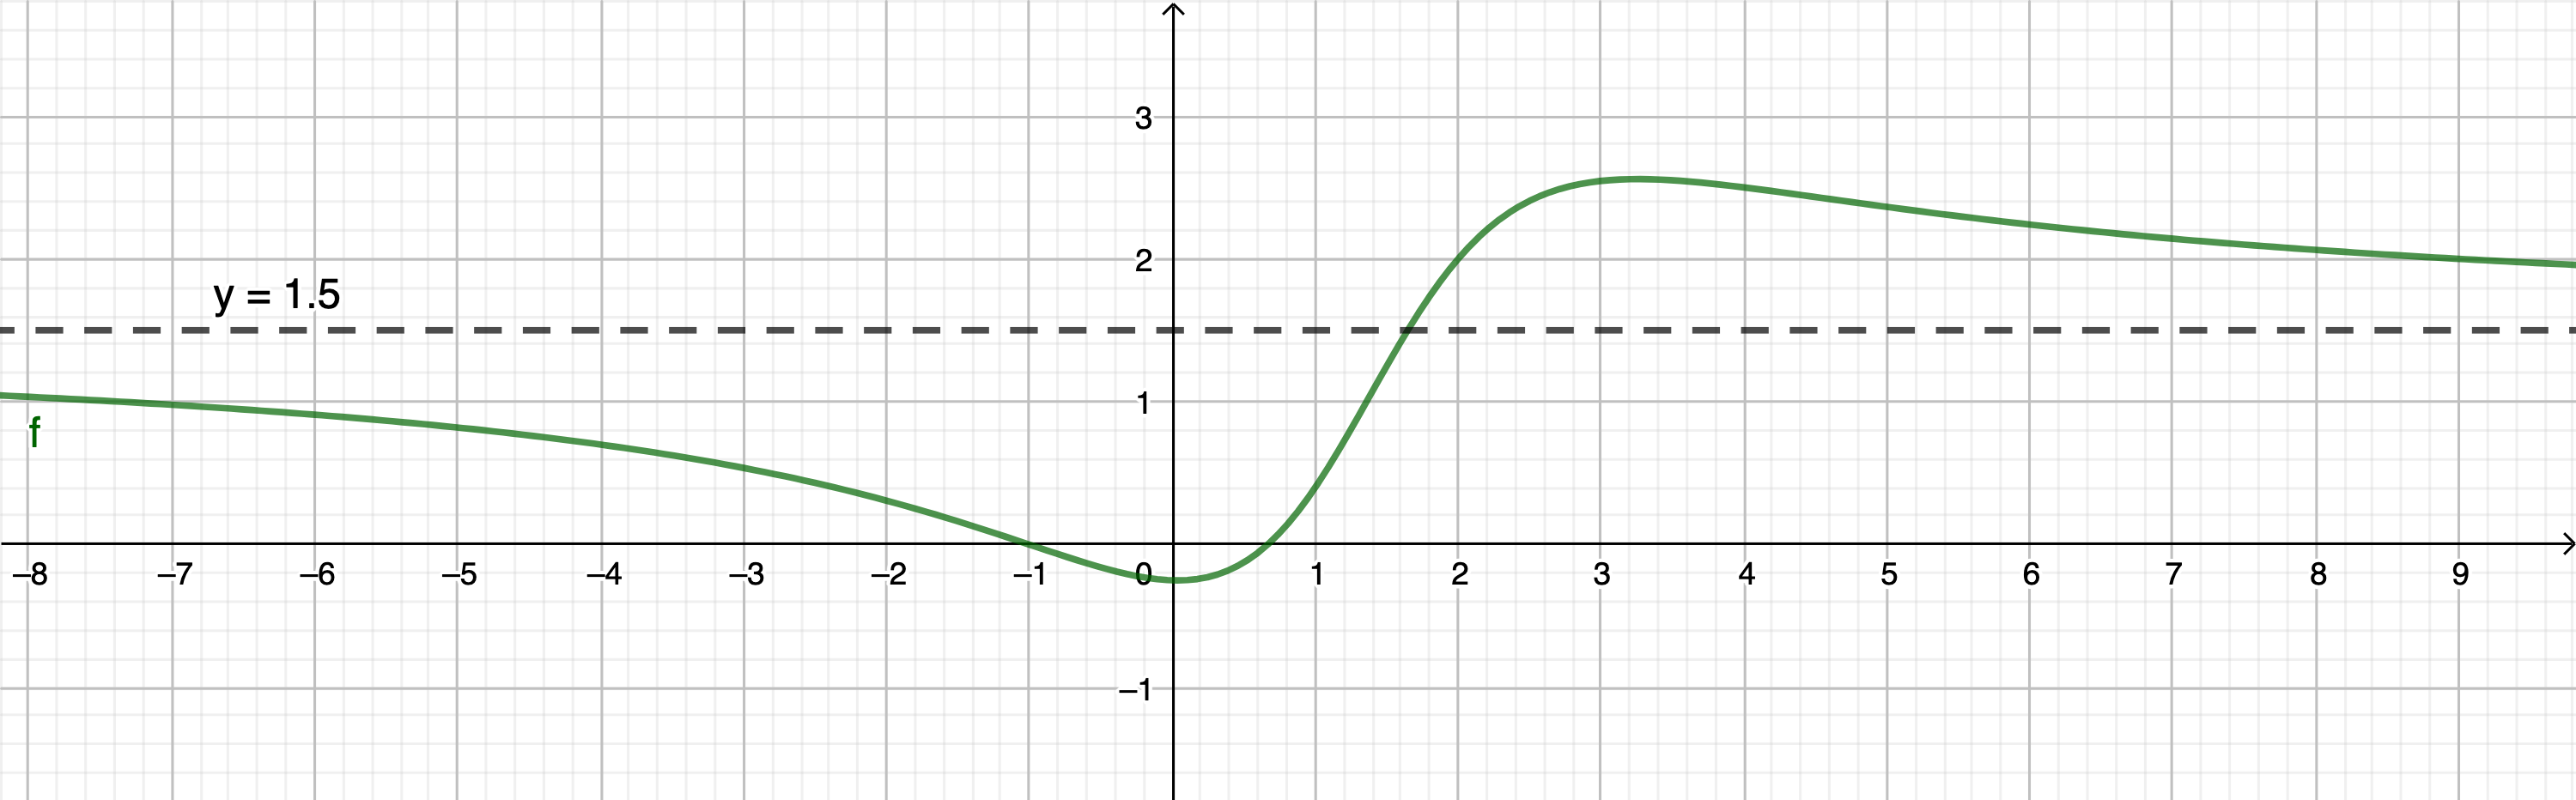
\includegraphics[scale=0.8]{media/introGrenzwertevonFu.png}
\end{center}
 
Ein Weg Gewissheit zu erlangen, ist eine Term-Analyse mit Hilfe einer Termumformung. Im konkreten Beispiel sieht das so aus:
$$f(x)=\frac{3x^2+x-2}{2x^2-5x+8}
=\frac{x^2\left(3+\frac{1}{x}-\frac{2}{x^2}\right)}{x^2 \left(2-\frac{5}{x}+\frac{8}{x^2}\right)}
=\frac{3+\frac{1}{x}-\frac{2}{x^2}}{2-\frac{5}{x}+\frac{8}{x^2}}$$ 

Für sehr grosse Werte von $x$ nähern sich die Terme $\frac{1}{x}, \frac{2}{x^2}, \frac{5}{x}$ und $\frac{8}{x^2}$  der Zahl $0$. Für $x\rightarrow\infty$ erhält man somit:
$$\lim_{x\rightarrow\infty} f(x) = \frac{3+0-0}{2-0+0} = \frac{3}{2}$$
Auf diese Art wird ersichtlich, dass sich die Funktion tatsächlich dem Grenzwert $1.5$ nähert.

Die Technik im Beispiel ist eine Anwendung der sogenannten Grenzwertsätzen:
 
\begin{satz}
    {Grenzwertsätze}{}
    Besitzen die Funktionen $f(x)$ und $g(x)$ Grenzwerte  für $x\rightarrow\infty$ so sind auch die Funktionen $f(x)\pm g(x),f(x)\cdot g(x)$ und, sofern $\lim\limits_{x\rightarrow\infty} g(x)\neq 0$, auch die Funktion $\frac{f(x)}{g(x)}$ konvergent.

Für die Grenzwerte gilt
$$\lim_{x\rightarrow\infty} (f(x) \pm g(x)) = \lim_{x\rightarrow\infty} f(x) \pm \lim_{x\rightarrow\infty}g(x)$$
$$\lim_{x\rightarrow\infty} (f(x) \cdot g(x)) = \lim_{x\rightarrow\infty} f(x) \cdot \lim_{x\rightarrow\infty}g(x)$$
$$\lim_{x\rightarrow\infty} \frac{f(x)}{g(x)} = \frac{\lim_{x\rightarrow\infty} f(x)}{\lim_{x\rightarrow\infty}g(x)}$$

Der Satz gilt auch für den Fall $x\rightarrow-\infty$
\end{satz}
Beweis: Siehe entsprechender Beweis im Kapitel „Folgen“...
\begin{ueb}
    {}{}
   \begin{enumerate}
    \item Bestimme, sofern vorhanden, den Grenzwert des Funktionsterms für $x \to \infty$.

    \begin{enumerate}
        \item $\lim\limits_{x \to \infty} \frac{x}{3x - 1}$
        \item $\lim\limits_{x \to \infty} \frac{1 - x^2}{x}$
        \item $\lim\limits_{x \to \infty} \frac{3x^7 - 4x^5}{2x^7 + 7x^6}$
        \item $\lim\limits_{x \to \infty} \frac{3 - x^3}{2x^3 + x^2}$
    \end{enumerate}
\item Welchen Wert hat $\lim\limits_{x \to \infty} f(x)$ und $\lim\limits_{x \to -\infty} f(x)$?

\begin{enumerate}
    \item $f(x) = \frac{2 + 3 \cdot 2^x}{2^x \cdot 4 - 1}$
    \item $f(x) = \frac{5^{-x} + 3}{8 - 2 \cdot 5^{-x}}$
\end{enumerate}

\item 
Berechne

\begin{enumerate}
    \item $\lim\limits_{x \to \infty} \frac{x^3 + \sin(x)}{x^3}$
    \item $\lim\limits_{x \to -\infty} \frac{x^2 - \sin(x)}{x^3}$
    \item $\lim\limits_{x \to \infty} \frac{\cos(x) - 3x}{1 - 2x}$
\end{enumerate}    
\item Bestimme die beiden Grenzwerte und vergleiche.

\begin{enumerate}
    \item $\lim\limits_{x \to \infty} \frac{2x^6 - 3x^5 + 7x^3 + 4x - 8}{5x^6 + 8x^5 - 9x^4 + 11x^2}$, \quad $\lim\limits_{x \to -\infty} \frac{2x^6 - 3x^5 + 7x^3 + 4x - 8}{5x^6 + 8x^5 - 9x^4 + 11x^2}$
    \item $\lim\limits_{x \to \infty} \frac{10x^8 - 4x^7 + 12}{x^9 + 3x^6 + 4}$, \quad $\lim\limits_{x \to -\infty} \frac{10x^8 - 4x^7 + 12}{x^9 + 3x^6 + 4}$
    \item  $\lim\limits_{x \to \infty} \frac{10x^8 - 4x^7 + 12}{x^7 + 3x^6 + 4}$, \quad $\lim\limits_{x \to -\infty} \frac{10x^8 - 4x^7 + 12}{x^7+ 3x^6 + 4}$
    \item   $\lim\limits_{x \to \infty} \frac{10x^8 - 4x^7 + 12}{ 3x^6 + 4}$, \quad $\lim\limits_{x \to -\infty} \frac{10x^8 - 4x^7 + 12}{3x^6 + 4}$
    \item $\lim\limits_{x \to \infty} \frac{\sqrt{x + 1}}{x - 1}$, \quad $\lim\limits_{x \to -\infty} \frac{\sqrt{x + 1}}{x - 1}$
    \item $\lim\limits_{x \to \infty} \frac{x^9 + x^4}{e^x}$, \quad $\lim\limits_{x \to -\infty} \frac{x^9 + x^4}{e^x}$
\end{enumerate}
\item Bestimme die Parameter $a, b$ und $c$ so, dass gilt:
    \[ \lim\limits_{x \to \infty} \frac{ax^b + 4x^5 + cx^3 - 1}{2x^3 - 11x^2 + 5} = 3. \]
\item  Gegeben ist der Funktionsterm $f(x) = \frac{4x^4 - 6x^3 + 7}{2x^m + 5x + 1}$. Bestimme den Exponenten $m \in \mathbb{N}_0$ so, dass die folgenden Grenzwerte resultieren, oder erkläre, weshalb es kein $m$ mit diesem Grenzwert gibt.
\begin{enumerate}
    \item $\lim\limits_{x \to \infty} f(x) = 2$
    \item $\lim\limits_{x \to \infty} f(x) = 0$
    \item $\lim\limits_{x \to -\infty} f(x) = -2$
    \item $\lim\limits_{x \to -\infty} f(x) = -\infty$
    \item $\lim\limits_{x \to -\infty} f(x) = \infty$
\end{enumerate}
   \end{enumerate}
\end{ueb}

\clearpage
\emph{Lösungen}
\begin{enumerate}
    \item 

\begin{enumerate}
    \item $\lim\limits_{x \to \infty} \frac{x}{3x - 1} = \frac{1}{3}$
    \item $\lim\limits_{x \to \infty} \frac{1 - x^2}{x} = -\infty$
    \item $\lim\limits_{x \to \infty} \frac{3x^7 - 4x^5}{2x^7 + 7x^6} = \frac{3}{2}$
    \item $\lim\limits_{x \to \infty} \frac{3 - x^3}{2x^3 + x^2} = -\frac{1}{2}$
\end{enumerate}

\item

\begin{enumerate}
    \item $f(x) = \frac{2 + 3 \cdot 2^x}{2^x \cdot 4 - 1}$, Grenzwert für $x\to \infty$: $\frac{3}{4}$, Grenzwert für $x\to-\infty$: $-2$
    \item $f(x) = \frac{5^{-x} + 3}{8 - 2 \cdot 5^{-x}}$, Grenzwert für $x\to \infty$: $\frac{3}{8}$, Grenzwert für $x\to-\infty$: $-\frac{1}{2}$
\end{enumerate}

\item

\begin{enumerate}
    \item $\lim\limits_{x \to \infty} \frac{x^3 + \sin(x)}{x^3} = 1$
    \item $\lim\limits_{x \to -\infty} \frac{x^2 - \sin(x)}{x^3} = 0$
    \item $\lim\limits_{x \to \infty} \frac{\cos(x) - 3x}{1 - 2x} = \frac{3}{2}$
\end{enumerate}

\item

\begin{enumerate}
    \item $\lim\limits_{x \to \infty} \frac{2x^6 - 3x^5 + 7x^3 + 4x - 8}{5x^6 + 8x^5 - 9x^4 + 11x^2} = \frac{2}{5}$, $\lim\limits_{x \to -\infty} \frac{2x^6 - 3x^5 + 7x^3 + 4x - 8}{5x^6 + 8x^5 - 9x^4 + 11x^2} = \frac{2}{5}$
    \item $\lim\limits_{x \to \infty} \frac{10x^8 - 4x^7 + 12}{x^9 + 3x^6 + 4} = 0$, $\lim\limits_{x \to -\infty} \frac{10x^8 - 4x^7 + 12}{x^9 + 3x^6 + 4} = 0$
    \item   $\lim\limits_{x \to \infty} \frac{10x^8 - 4x^7 + 12}{x^7 + 3x^6 + 4} = \infty$, \quad $\lim\limits_{x \to -\infty} \frac{10x^8 - 4x^7 + 12}{x^7+ 3x^6 + 4}=- \infty$
    \item   $\lim\limits_{x \to \infty} \frac{10x^8 - 4x^7 + 12}{ 3x^6 + 4}= \infty$, \quad $\lim\limits_{x \to -\infty} \frac{10x^8 - 4x^7 + 12}{3x^6 + 4}= \infty$
    \item $\lim\limits_{x \to \infty} \frac{\sqrt{x + 1}}{x - 1} = 0$, $\lim\limits_{x \to -\infty} \frac{\sqrt{x + 1}}{x - 1}$ gibt es nicht 
    \item $\lim\limits_{x \to \infty} \frac{x^9 + x^4}{e^x} = 0$, $\lim\limits_{x \to -\infty} \frac{x^9 + x^4}{e^x} = -\infty$
\end{enumerate}

\item $a = -4$, $b = 5$, $c = 6$.

\item    \begin{enumerate}
        \item $\lim\limits_{x \to \infty} f(x) = 2$, Lösung: $m = 4$
        \item $\lim\limits_{x \to \infty} f(x) = 0$, Lösung:  $m>4$ 
        \item $\lim\limits_{x \to -\infty} f(x) = -2$, Lösung: nicht möglich
        \item $\lim\limits_{x \to -\infty} f(x) = -\infty$, Lösung: $m\in \{0, 1, 3\}$
        \item $\lim\limits_{x \to -\infty} f(x) = \infty$, Lösung: $m =2$
    \end{enumerate}

\end{enumerate}














\clearpage
\subsubsection{Grenzwert einer Funktion an einer Stelle \texorpdfstring{$a\in \R$}{a}}
\begin{LA}
    {Einführungsaufgabe}{}
    Untersuchen Sie die Funktion $f(x)=\frac{x^3+10x^2-24x}{7x-14}$. 
        \begin{enumerate}
            \item Wieso ist die Funktion an der Stelle $x=2$ nicht definiert?
            \item Zeichnen Sie die Funktion mit \href{https://www.geogebra.org/calculator}{Geogebra}
            \item Definieren Sie in Geogebra einen `Laufpunkt' auf dem Graphen von $f$, indem Sie P=(a, f(a)) tippen. Geogebra erstellt automatisch einen Schieberegler, mit dem Sie die $x$-Koordinate von $P$ verändern können.
            \item  Beobachten Sie, was mit $P$ passiert, wenn $a$ sich der Zahl 2 nähert.
            \item  Was vermuten Sie ist der Wert des Grenzwertes $\lim\limits_{x\to 2} f(x)$?
            \item  Wie kann man diesen Grenzwert anhand der Funktionsgleichung berechnen?
            %\item  Wenn man etwas rauszoomt, sieht man, dass der Graph von $f$ eine bekannte Form hat. Können Sie das anhand der Funktionsgleichung erklären?
        \end{enumerate}



    % \begin{enumerate}
    %     \item Berechnen Sie einige Werte und füllen Sie die Wertetabelle: \newline
    %     \begin{center}
    %         \begin{tabular}{c||c|c|c|c}
    %             $x$ & $0$ & $1$ & $2$ & $3$ \\ \hline
    %         $f(x)$    &&&&   
    %         \end{tabular}
                  
    %     \end{center}
    %     \item Wie erklären Sie sich das spezielle Resultat?
    %     \item Füllen Sie auch die folgende Wertetabelle aus:
    %     \begin{center}
    %         \begin{tabular}{c||c|c|c|c}
    %             $x$ & $1.9$ & $1.99$ & $2.01$ & $2.1$ \\ \hline
    %         $f(x)$    &&&&   
    %         \end{tabular}
                  
    %     \end{center}
    %     \item 	Zeichnen Sie die Funktion mit Geogebra: 
    %     \begin{enumerate}
    %         \item Definieren Sie in Geogebra einen «Laufpunkt» auf dem Graphen von $f$, indem Sie P=(a, f(a)) tippen. Geogebra erstellt so automatisch einen Schieberegler, mit dem Sie die $x$-Koordinate von $P$ verändern können.
    %         \item  Beobachten Sie was mit $P$ passiert, wenn $a$ sich der Zahl 2 nähert.
    %         \item  Wenn man etwas rauszoomt, sieht man, dass der Graph von $f$ eine bekannte Form hat. Können Sie das anhand der Funktionsgleichung erklären?
    %     \end{enumerate}
        
    % \end{enumerate}
\end{LA}
\newpage
Mit der Einführungsaufgabe haben wir ein Beispiel dafür, wie man sich den Grenzwert einer Funktion für $x$ gegen eine Zahl vorstellen muss. Auch für diesen Grenzwertbegriff gibt es eine präzise, mathematische Definition, wir verzichten aber hier vorerst darauf und beschränken uns auf eine etwas ungenauere, dafür verständlichere Variante:

\begin{definition}
    {Grenzwert einer Funktion an einer Stelle $a\in \R$}{}
Eine Zahl $g$ heisst Grenzwert der Funktion $f$ für $x$ gegen $a$, falls alle Funktionswerte $f(x)$ beliebig wenig von $g$ abweichen, sobald $x$ entsprechend nahe bei $a$ liegt, aber verschieden von $a$ ist.
Notation:
$$\lim_{x\rightarrow a} f(x) = g$$
\end{definition}


Betrachten wir noch einmal das Einführungsbeispiel. Die Wertetabelle lässt vermuten, dass der Grenzwert $\lim\limits_{x\rightarrow 2} \frac{x^3+10x^2-24x}{7x-14} =4$ ist. Wie kann man aber Gewissheit erlangen? Schliesslich haben wir nur die Werte an den Stellen $1.99$ und $2.01$ betrachtet, aber es gibt Zahlen, die sich um viel weniger von $2$ unterscheiden – zum Beispiel $x=2+10^{-1000000000}$. 

Wieder hilft uns eine Termumformung:
$$\frac{x^3+10x^2-24x}{7x-14} = \frac{x(x^2+10x-24)}{7(x-2)} = \frac{x(x-2)(x+12)}{7(x-2)}\stackrel{x\neq 2}{=}\frac{x(x+12)}{7}$$

Die beiden Terme ganz links und ganz rechts liefern für alle Werte von $x$ das gleiche Resultat mit einer Ausnahme: Für $x=2$ ist der Term links nicht definiert, der rechts aber schon. Bildlich gesprochen stimmen die Graphen der beiden Funktionen $f(x)=\frac{x^3+10x^2-24x}{7x-14}$ und $g(x)=\frac{x(x+12)}{7}$ überall überein – nur das der Graph von $f$ an der Stelle $x=2$ ein Loch aufweist, während jener von $g$ durchgängig ist. 
Damit gilt
$$\lim_{x\rightarrow2} \frac{x^3+10x^2-24x}{7x-14} = \lim_{x\rightarrow2} \frac{x(x+12)}{7} =\frac{2\cdot (2+12)}{7} = 4$$

\begin{ueb}
    {}{}
    Bestimme den Grenzwert

    % \begin{enumerate}
    %     \item $\lim\limits_{x \to 2} \frac{4-x^2}{2 - x}$
    %     \item $\lim\limits_{x \to 1} \frac{10x^2 - 10}{1 - x}$
    %     \item $\lim\limits_{x \to 3} \frac{8x - 24}{x^2 - 9}$
    %     \item $\lim\limits_{x \to -2} \frac{x^2 + 3x + 2}{x^2 + 2x}$
    %     \item $\lim\limits_{x \to 1} \frac{x^2 + 1}{x - 2}$
    %     \item $\lim\limits_{x \to 0} \frac{x^2 - 1}{x - 2}$
    %     \item $\lim\limits_{x \to 2} \frac{x^2 - 4}{x - 2}$
    %     \item $\lim\limits_{x \to -4} \frac{x - 2}{x^2 - 4}$
    %     \item $\lim\limits_{x \to 3} \frac{x^2 - 4x + 3}{x^2 - 9}$
    %     \item $\lim\limits_{x \to 1} \frac{x^2 - 4x + 3}{x^2 - 9}$
    % \end{enumerate}

    \begin{enumerate}
        \item $\lim\limits_{x \to 1} \frac{x^2 + 4x - 5}{x^2 - 1}$
        \item $\lim\limits_{x \to 1} \frac{x^2 + 4x - 5}{x^2 - 2x + 1}$
        \item $\lim\limits_{x \to -9} \frac{x^2 + 7x - 18}{x^2 - 81}$
        \item $\lim\limits_{x \to -4} \frac{x + 6}{x^2 - 4}$
        \item $\lim\limits_{x \to -2} \frac{12x^2 + 24x}{x^2 + 10x + 16}$
        \item $\lim\limits_{x \to 2} \frac{3x^2 - 6x}{6 - 5x + x^2}$
        \item $\lim\limits_{x \to 4} \frac{2x^2 - 14x + 24}{12x - 7x^2 + x^3}$
    \end{enumerate}
\end{ueb}
\clearpage
\emph{Lösungen}
% \begin{enumerate}
%     \item $\-4$
%     \item $\lim\limits_{x \to 1} \frac{10(x - 1)(x + 1)}{1 - x} = -10(1 + 1) = -20$
%     \item $\lim\limits_{x \to 3} \frac{8(x - 3)}{x^2 - 9} = \frac{8(3-3)}{9-9} = \text{nicht definiert}$
%     \item $\lim\limits_{x \to -2} \frac{x^2 + 3x + 2}{x^2 + 2x} = \frac{4 - 6 + 2}{4 - 4} = \text{nicht definiert}$
%     \item $\lim\limits_{x \to 1} \frac{x^2 + 1}{x - 2} = \frac{1 + 1}{1 - 2} = -2$
%     \item $\lim\limits_{x \to 0} \frac{x^2 - 1}{x - 2} = \frac{0 - 1}{-2} = \frac{1}{2}$
%     \item $\lim\limits_{x \to 2} \frac{x^2 - 4}{x - 2} = \lim\limits_{x \to 2} (x+2) = 4$
%     \item $\lim\limits_{x \to -4} \frac{x - 2}{x^2 - 4} = \frac{-4 - 2}{16 - 4} = \frac{-6}{12} = -\frac{1}{2}$
%     \item $\lim\limits_{x \to 3} \frac{x^2 - 4x + 3}{x^2 - 9} = \frac{9 - 12 + 3}{9 - 9} = \text{nicht definiert}$
%     \item $\lim\limits_{x \to 1} \frac{x^2 - 4x + 3}{x^2 - 9} = \frac{1 - 4 + 3}{1 - 9} = \frac{0}{-8} = 0$
% \end{enumerate}

\begin{enumerate}
    \item $3$
    \item unbestimmt divergent $\pm\infty$
    \item $\frac{11}{18}$
    \item $\frac{1}{6}$
    \item $-4$
    \item $-6$
    \item $1/2$
\end{enumerate}
















\clearpage

\subsubsection{Linksseitige und rechtsseitige Grenzwerte, Stetigkeit}

\begin{LA}{Einführungsaufgabe}{}
    Wir untersuchen die Funktion:
    $$f(x) = x\cdot \sqrt{1+\frac{1}{x^2}}$$

    \begin{enumerate}
        \item An welcher Stelle ist die Funktion nicht definiert?
        \item Was passiert, wenn $x$ sich der Definitionslücke nähert?
        \item Zeichnen Sie den Graphen von $f$ mit Geogebra und fügen Sie ihn hier unten an (Wurzeln können mit dem Befehl \glqq sqrt\grqq{} oder mit \glqq hoch 0.5\grqq{} eingegeben werden). 
    \end{enumerate}
\end{LA}
\clearpage
Für die Funktion aus der Einführungsaufgabe gilt: Je nachdem ob $x$ von links oder rechts gegen $0$ strebt, strebt der Funktionswert gegen $-1$ oder $+1$. Man spricht in diesem Fall vom links- bzw. rechtsseitigen Grenzwert und schreibt:
$$\lim_{x\uparrow 0} f(x) = -1 \quad \mathrm{oder}  \lim_{x\rightarrow 0^-} f(x) = -1 $$
beziehungsweise
$$\lim_{x\downarrow 0} f(x) = 1 \quad \mathrm{oder}  \lim_{x\rightarrow 0^+} f(x) = 1 $$

Für Funktionen gibt es an einer bestimmten Stelle drei mögliche Grenzwerte: der linksseitige, der rechtsseitige und DER Grenzwert. Der folgende Satz erklärt den Zusammenhang zwischen den drei Arten:

\begin{satz}{Zusammenhang zwischen den Grenzwerten}{}
Wenn der links- und der rechtsseitige Grenzwert übereinstimmen, dann existiert auch DER Grenzwert und es gilt:
$$\lim_{x\uparrow a} f(x) = \lim_{x\downarrow a} f(x) = \lim_{x\rightarrow a} f(x) $$

Wenn links- und rechtsseitige Grenzwerte \emph{nicht} übereinstimmen, dann existiert DER Grenzwert nicht.
$$\lim_{x\uparrow a} f(x) \neq \lim_{x\downarrow a} f(x) \Rightarrow  \lim_{x\rightarrow a} f(x) \text{ existiert nicht}$$
\end{satz}

\begin{bsp}
    {}{}
    Die Aufrundungsfunktion $x\mapsto \left \lceil{x}\right \rceil $ rundet jede Zahl $x$ auf die kleinste ganze Zahl, die grösser oder gleich $x$ ist.

    $\lim_{x\uparrow 42} \lceil x\rceil = ? , \quad \lim_{x\downarrow 42} \lceil x\rceil = ? $, Graph?
    
    \vspace{9cm}
\end{bsp}
\clearpage
Die Aufrundungsfunktion ist ein Beispiel für eine Funktion, die an gewissen Stellen Sprünge aufweist. Die meisten Funktionen, die Sie bisher angetroffen haben, hatten keine solche Sprungstellen. Wenn eine Funktion keine Sprungstelle hat, nennt man sie stetig. Genauer:

\begin{definition}{}{}
    Eine Funktion mit Definitionsbereich $\mathbb{D}$  heisst \emph{stetig an der Stelle $a\in \mathbb{D}$}, wenn
    $$ \lim_{x\uparrow a} f(x) = \lim_{x\downarrow a} f(x) = f(a)$$
\end{definition}
\begin{bsp}{}{}
    \begin{enumerate}
        \item Die Quadratfunktion $f(x)=x^2$ ist stetig. Der Graph weist keinerlei Sprungstellen auf.
        \begin{center}
            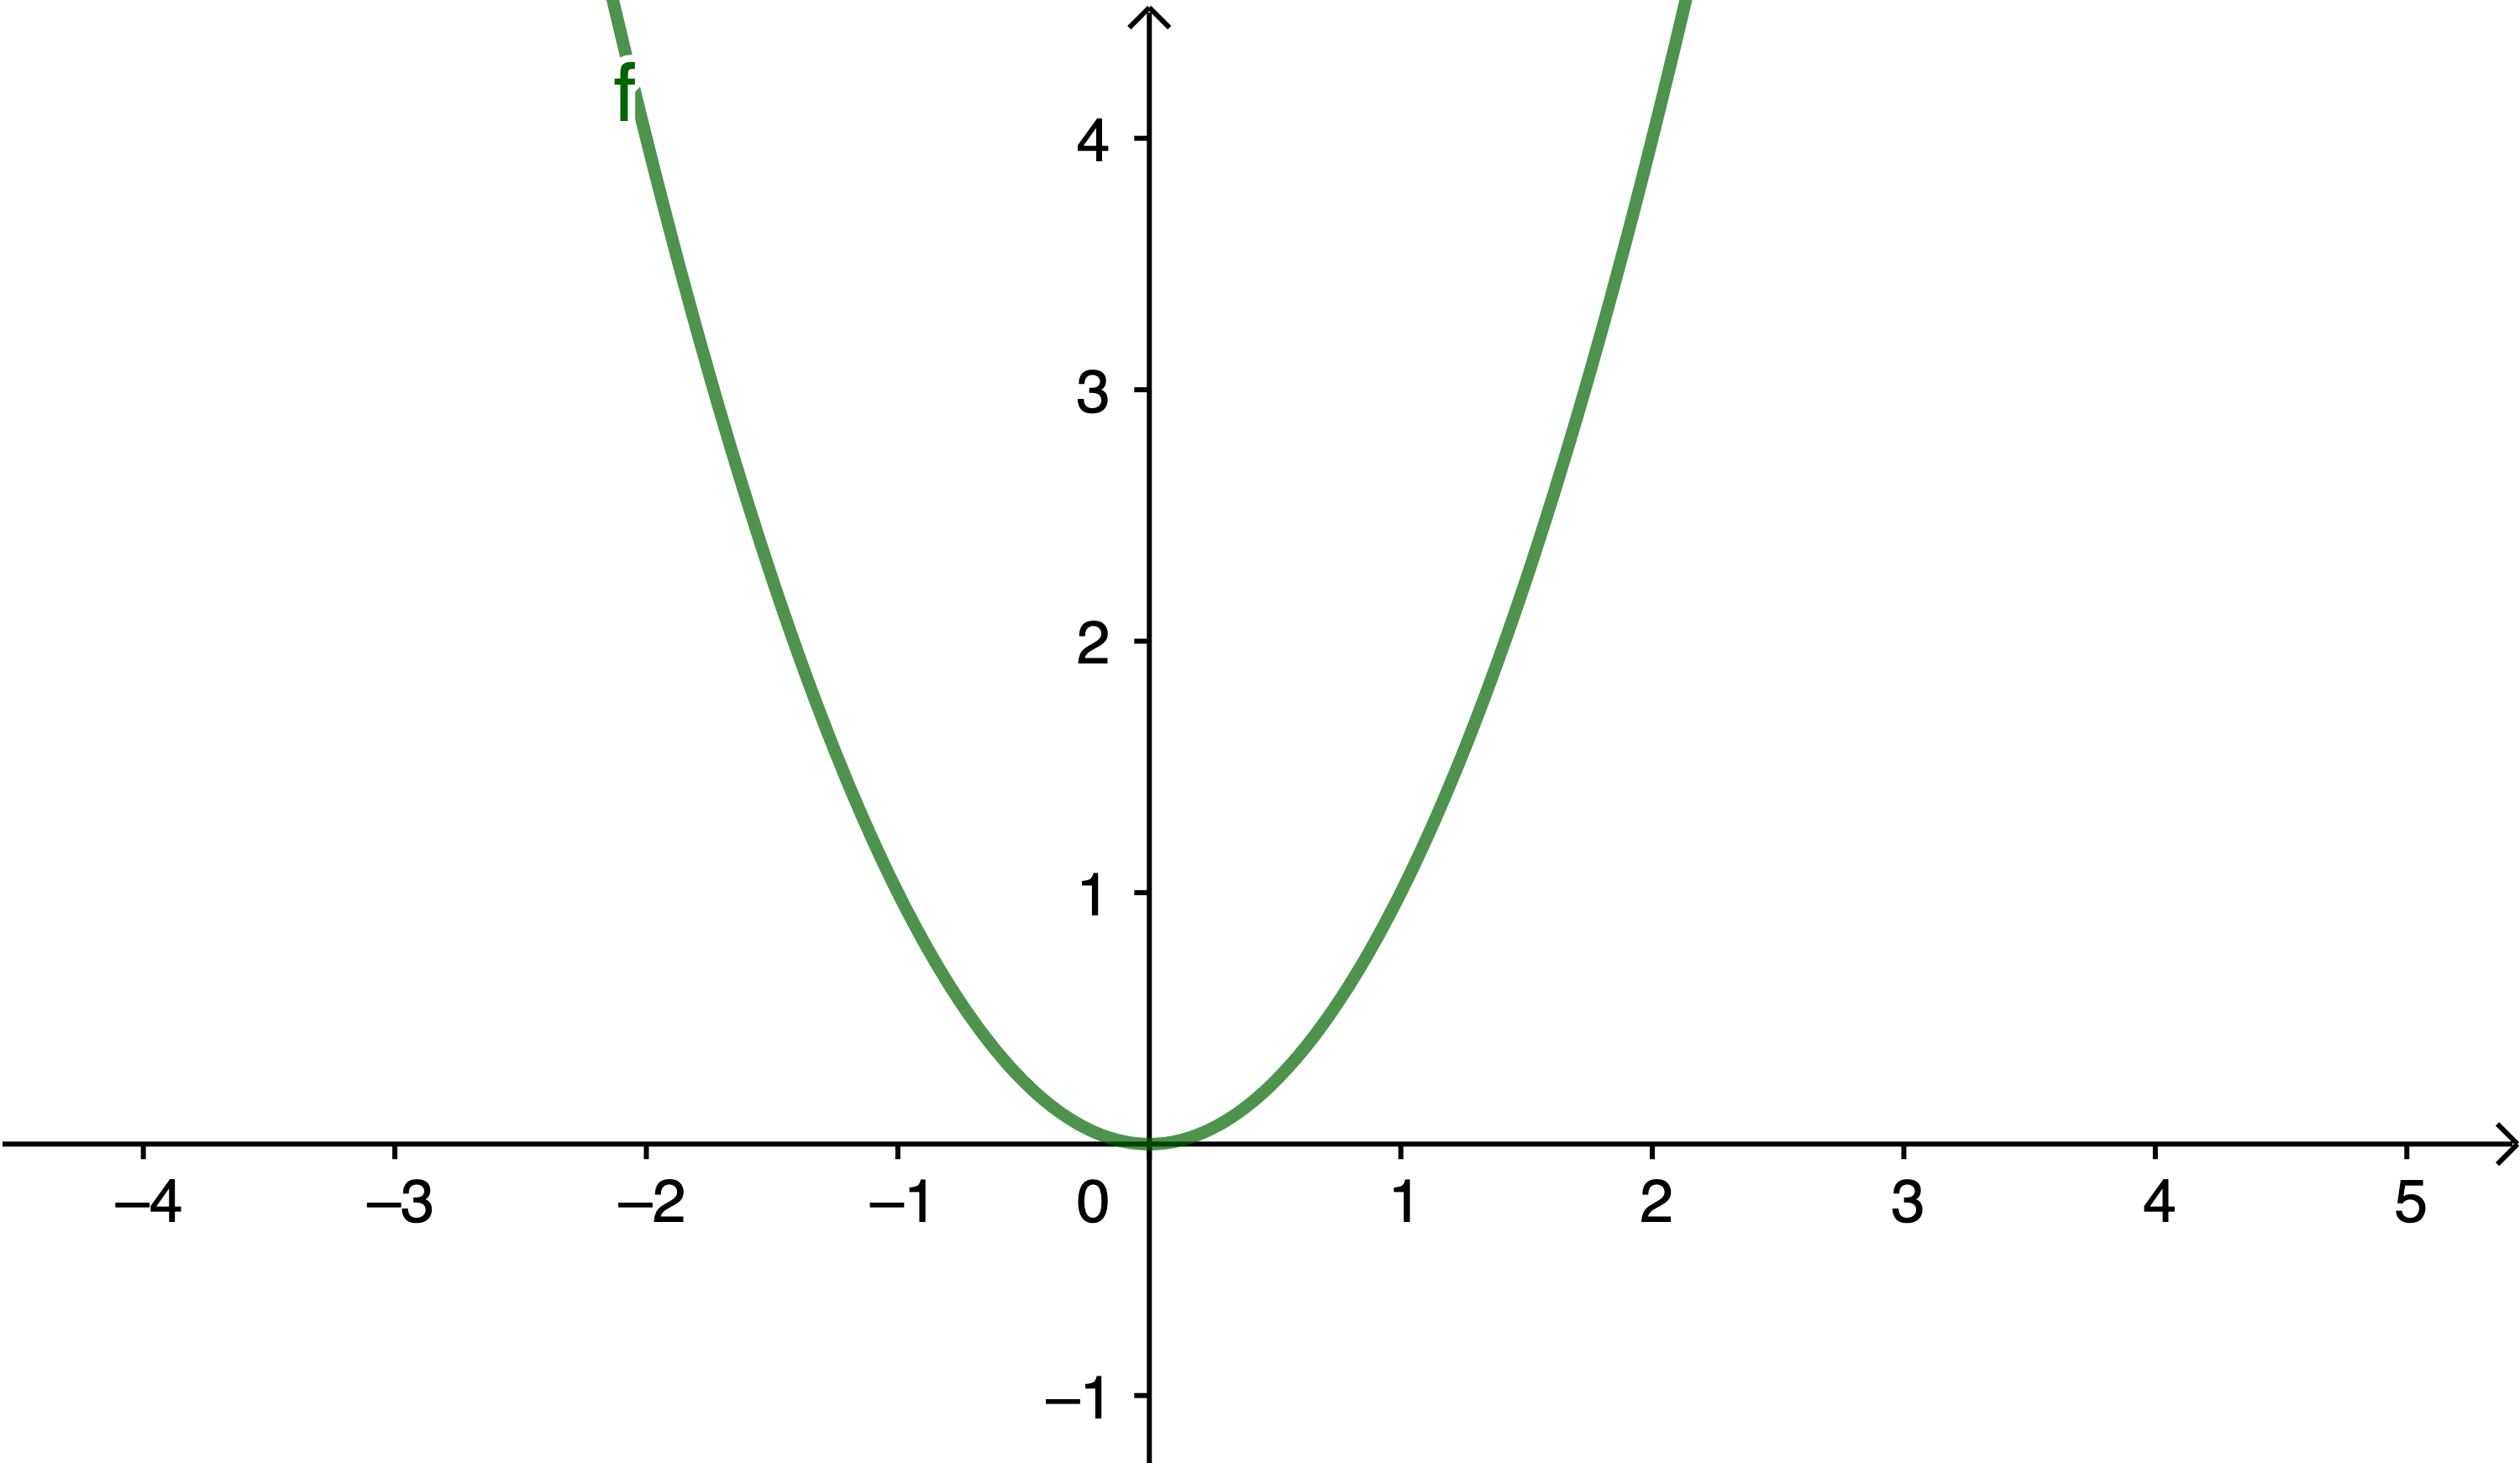
\includegraphics[scale=0.8]{media/quadratfunktion.png}
        \end{center}
    \item Die Vorzeichenfunktion 
    $$ \mathrm{sgn}(x)=\begin{cases}
        1, \quad \text{falls } x>0 \\
        0, \quad \text{falls } x=0 \\
        -1, \quad \text{falls } x<0
    \end{cases}$$
    ist nicht stetig, weil $$\lim_{x\uparrow 0} f(x) = -1 \neq \lim_{x\downarrow 0} f(x) = 1$$
    \begin{center}
        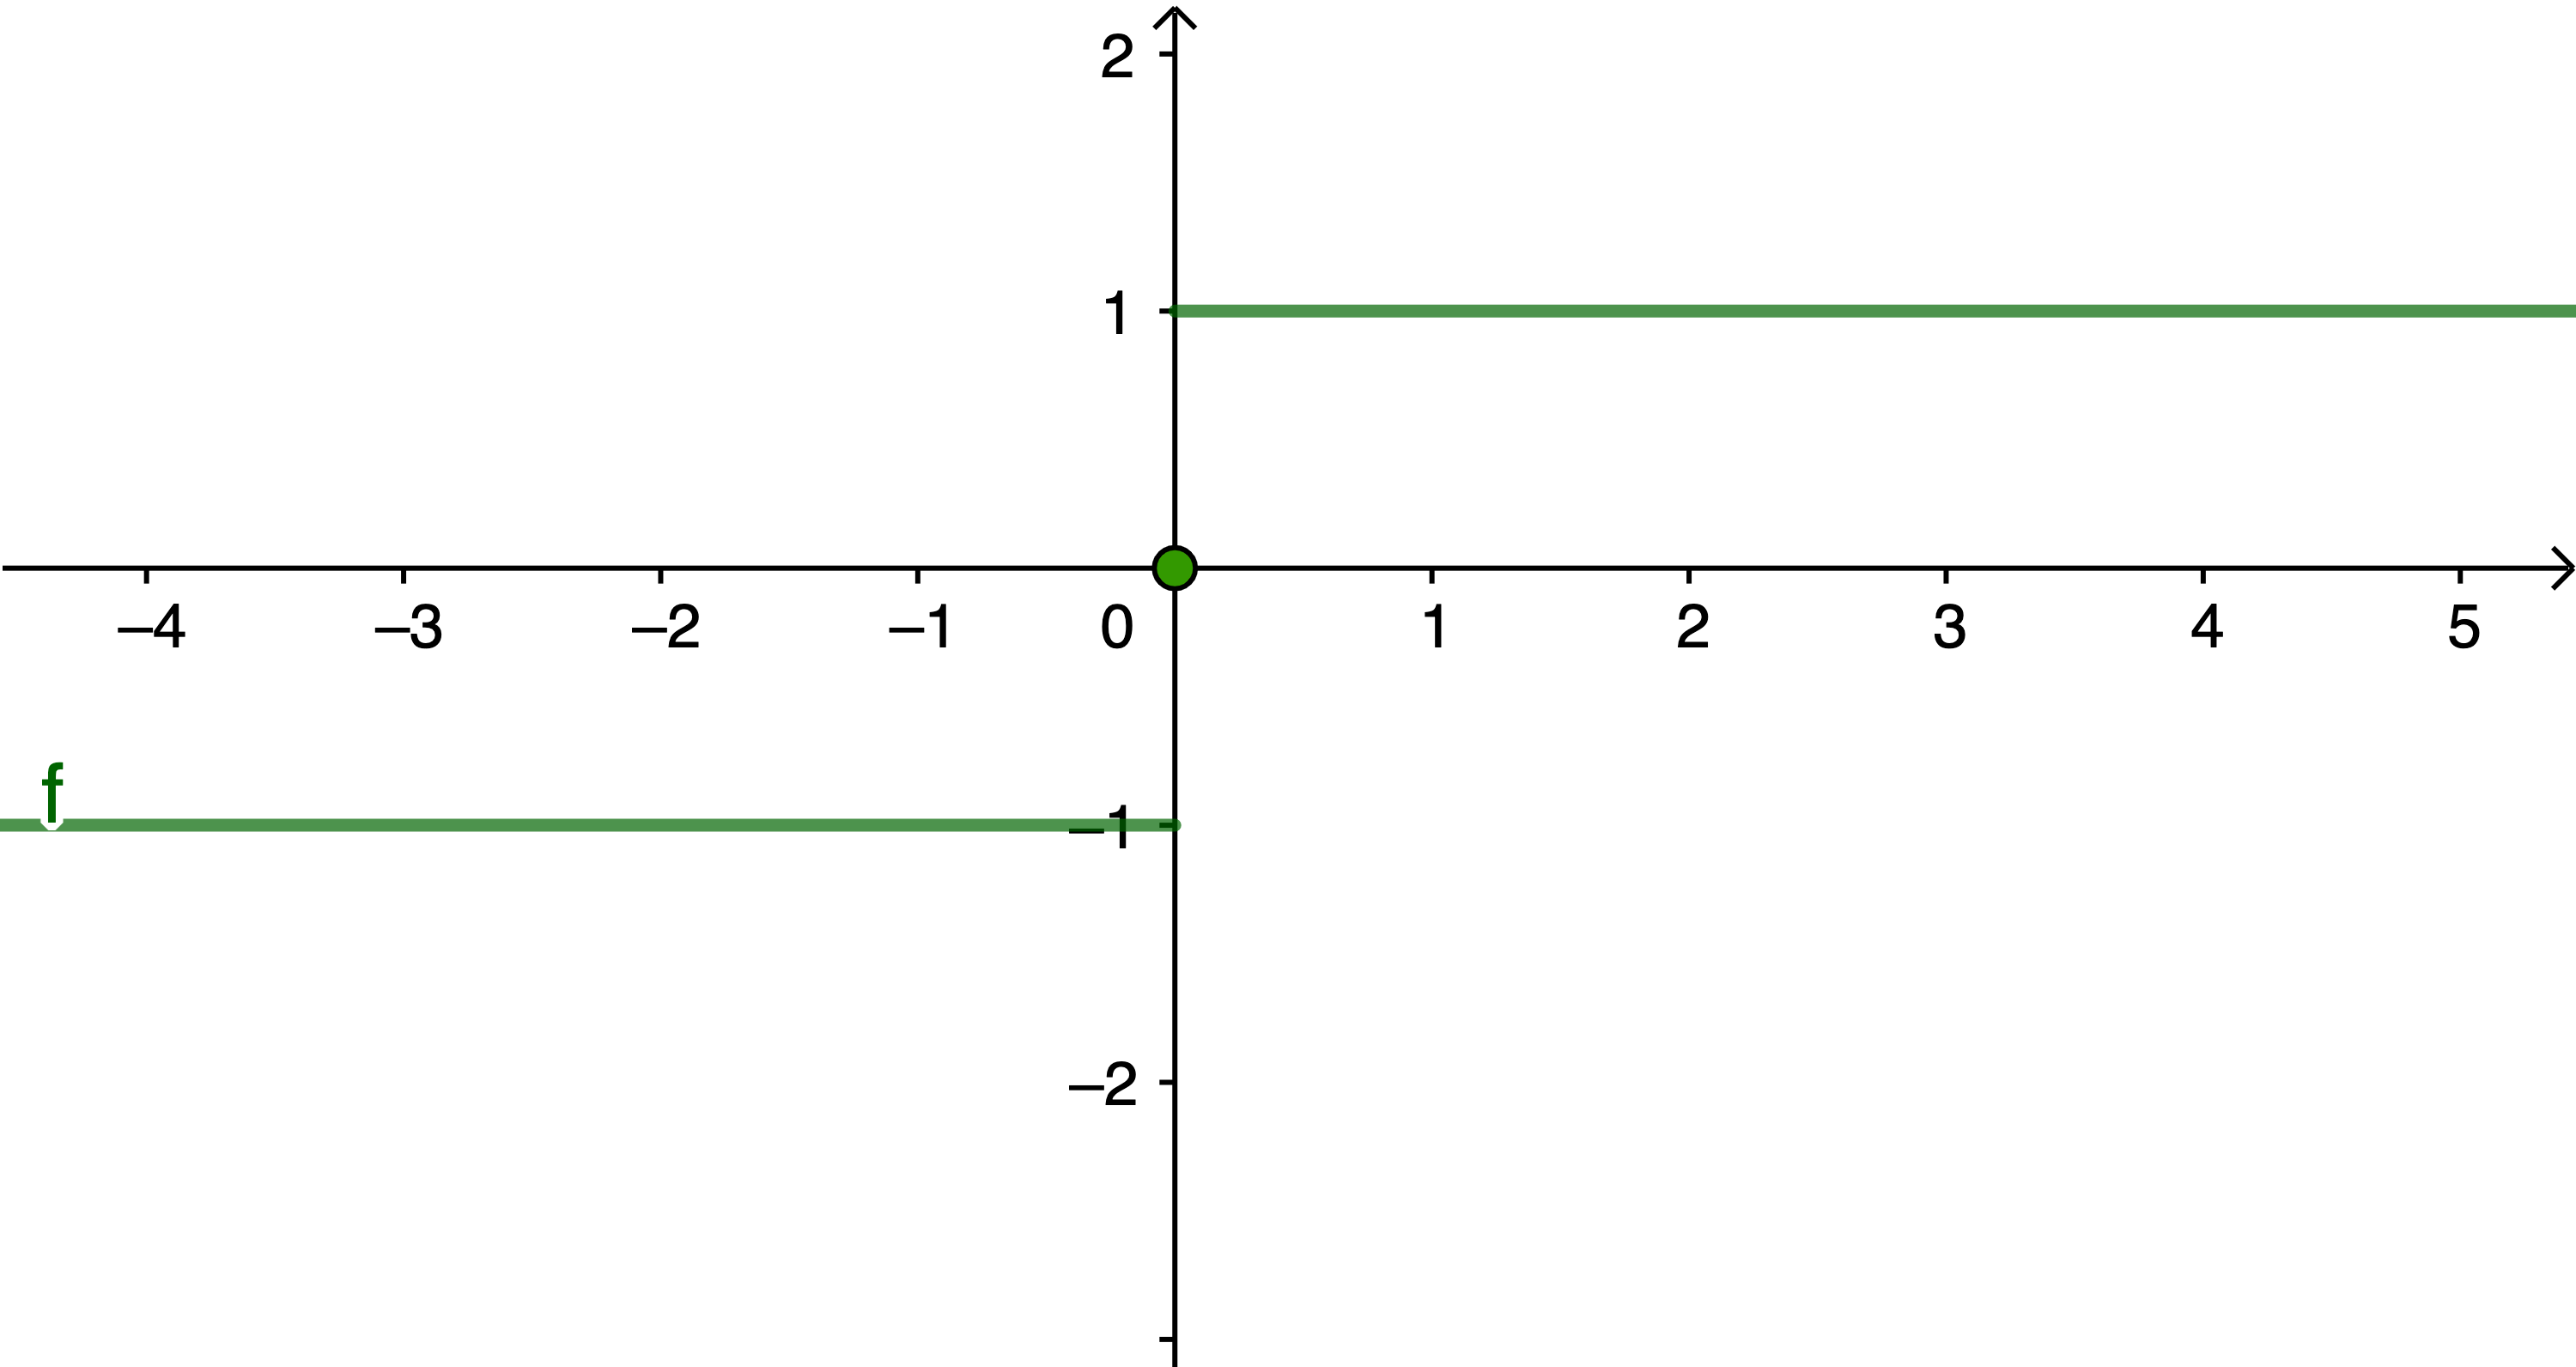
\includegraphics[scale=0.8]{media/sgn.png}
    \end{center}
    \pagebreak
    \item Die Betragsfunktion
    $$|x| = \begin{cases}
        x\quad \text{falls } x\le0 \\
        -x, \quad \text{falls } x<0 
    \end{cases}
    $$
    ist stetig. Der Graph hat zwar einen Ecke, aber keine \glqq Sprungstelle\grqq{}.
    \begin{center}
        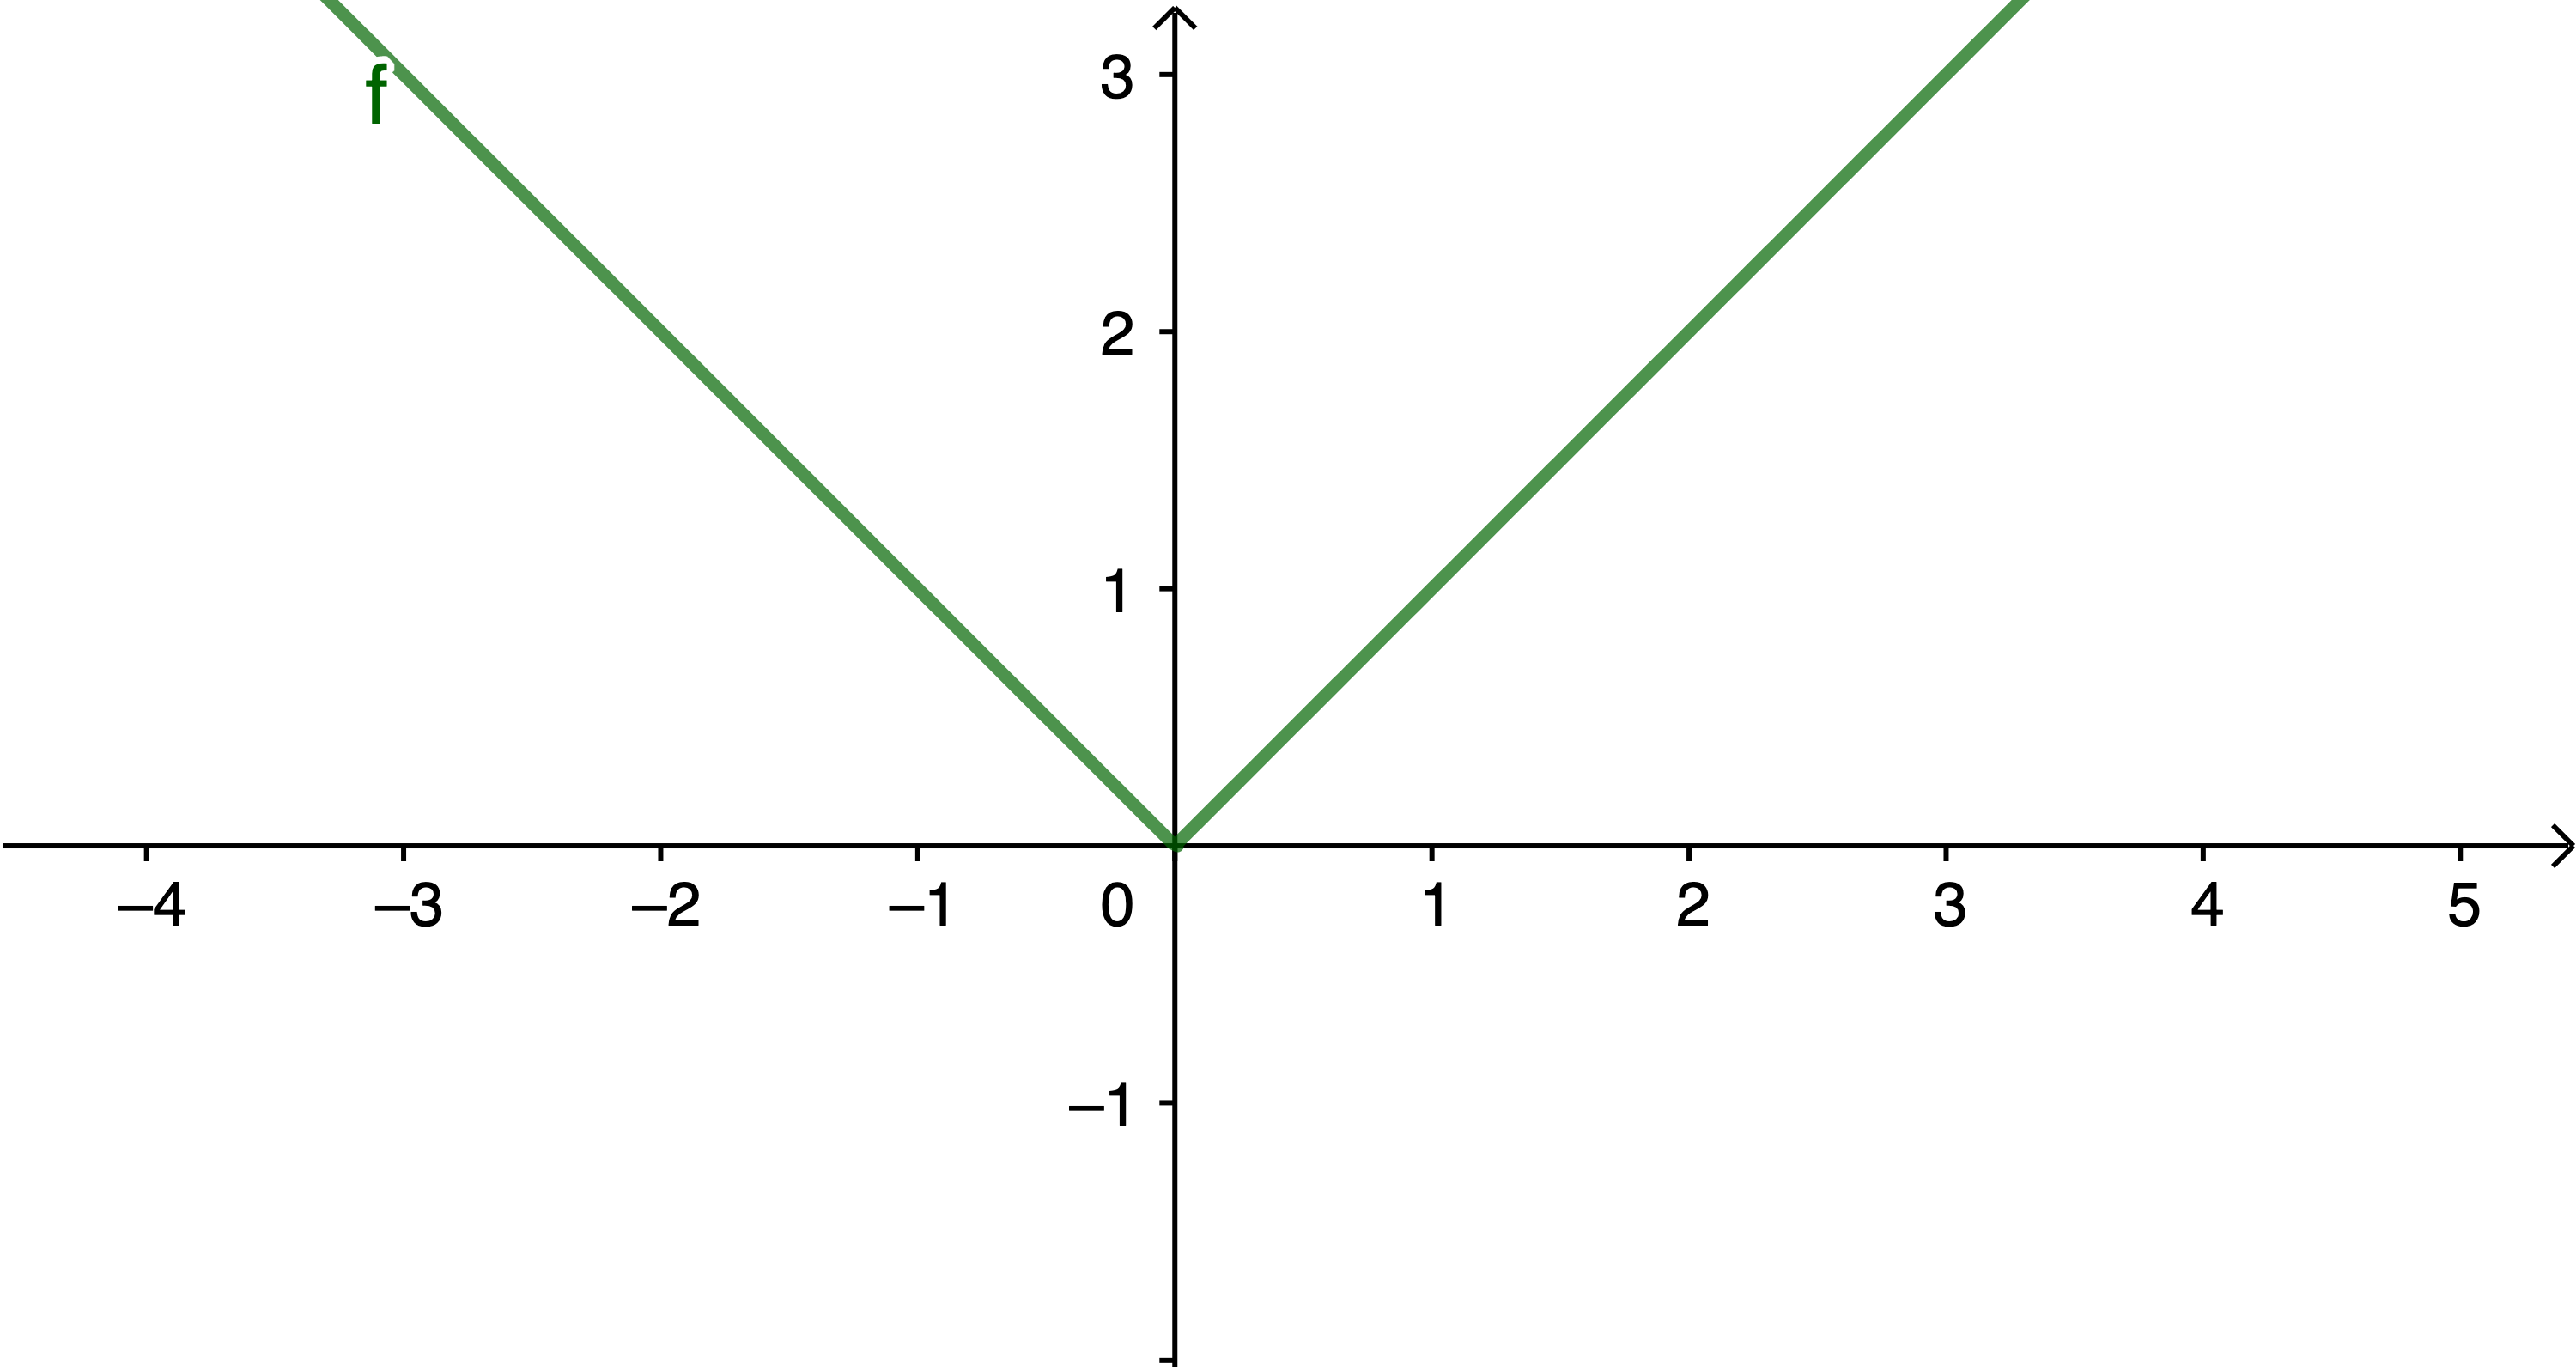
\includegraphics[scale=0.8]{media/abs.png}
    \end{center}
    \item 	Die Kehrwertfunktion  $p(x)=\frac{1}{x}$ ist trotz des Sprungs von $-\infty$ nach $+\infty$ stetig, weil die vermeintliche Sprungstelle $x=0$ ausserhalb des Definitionsbereichs $\mathbb{D}_p$ liegt.
    \begin{center}
        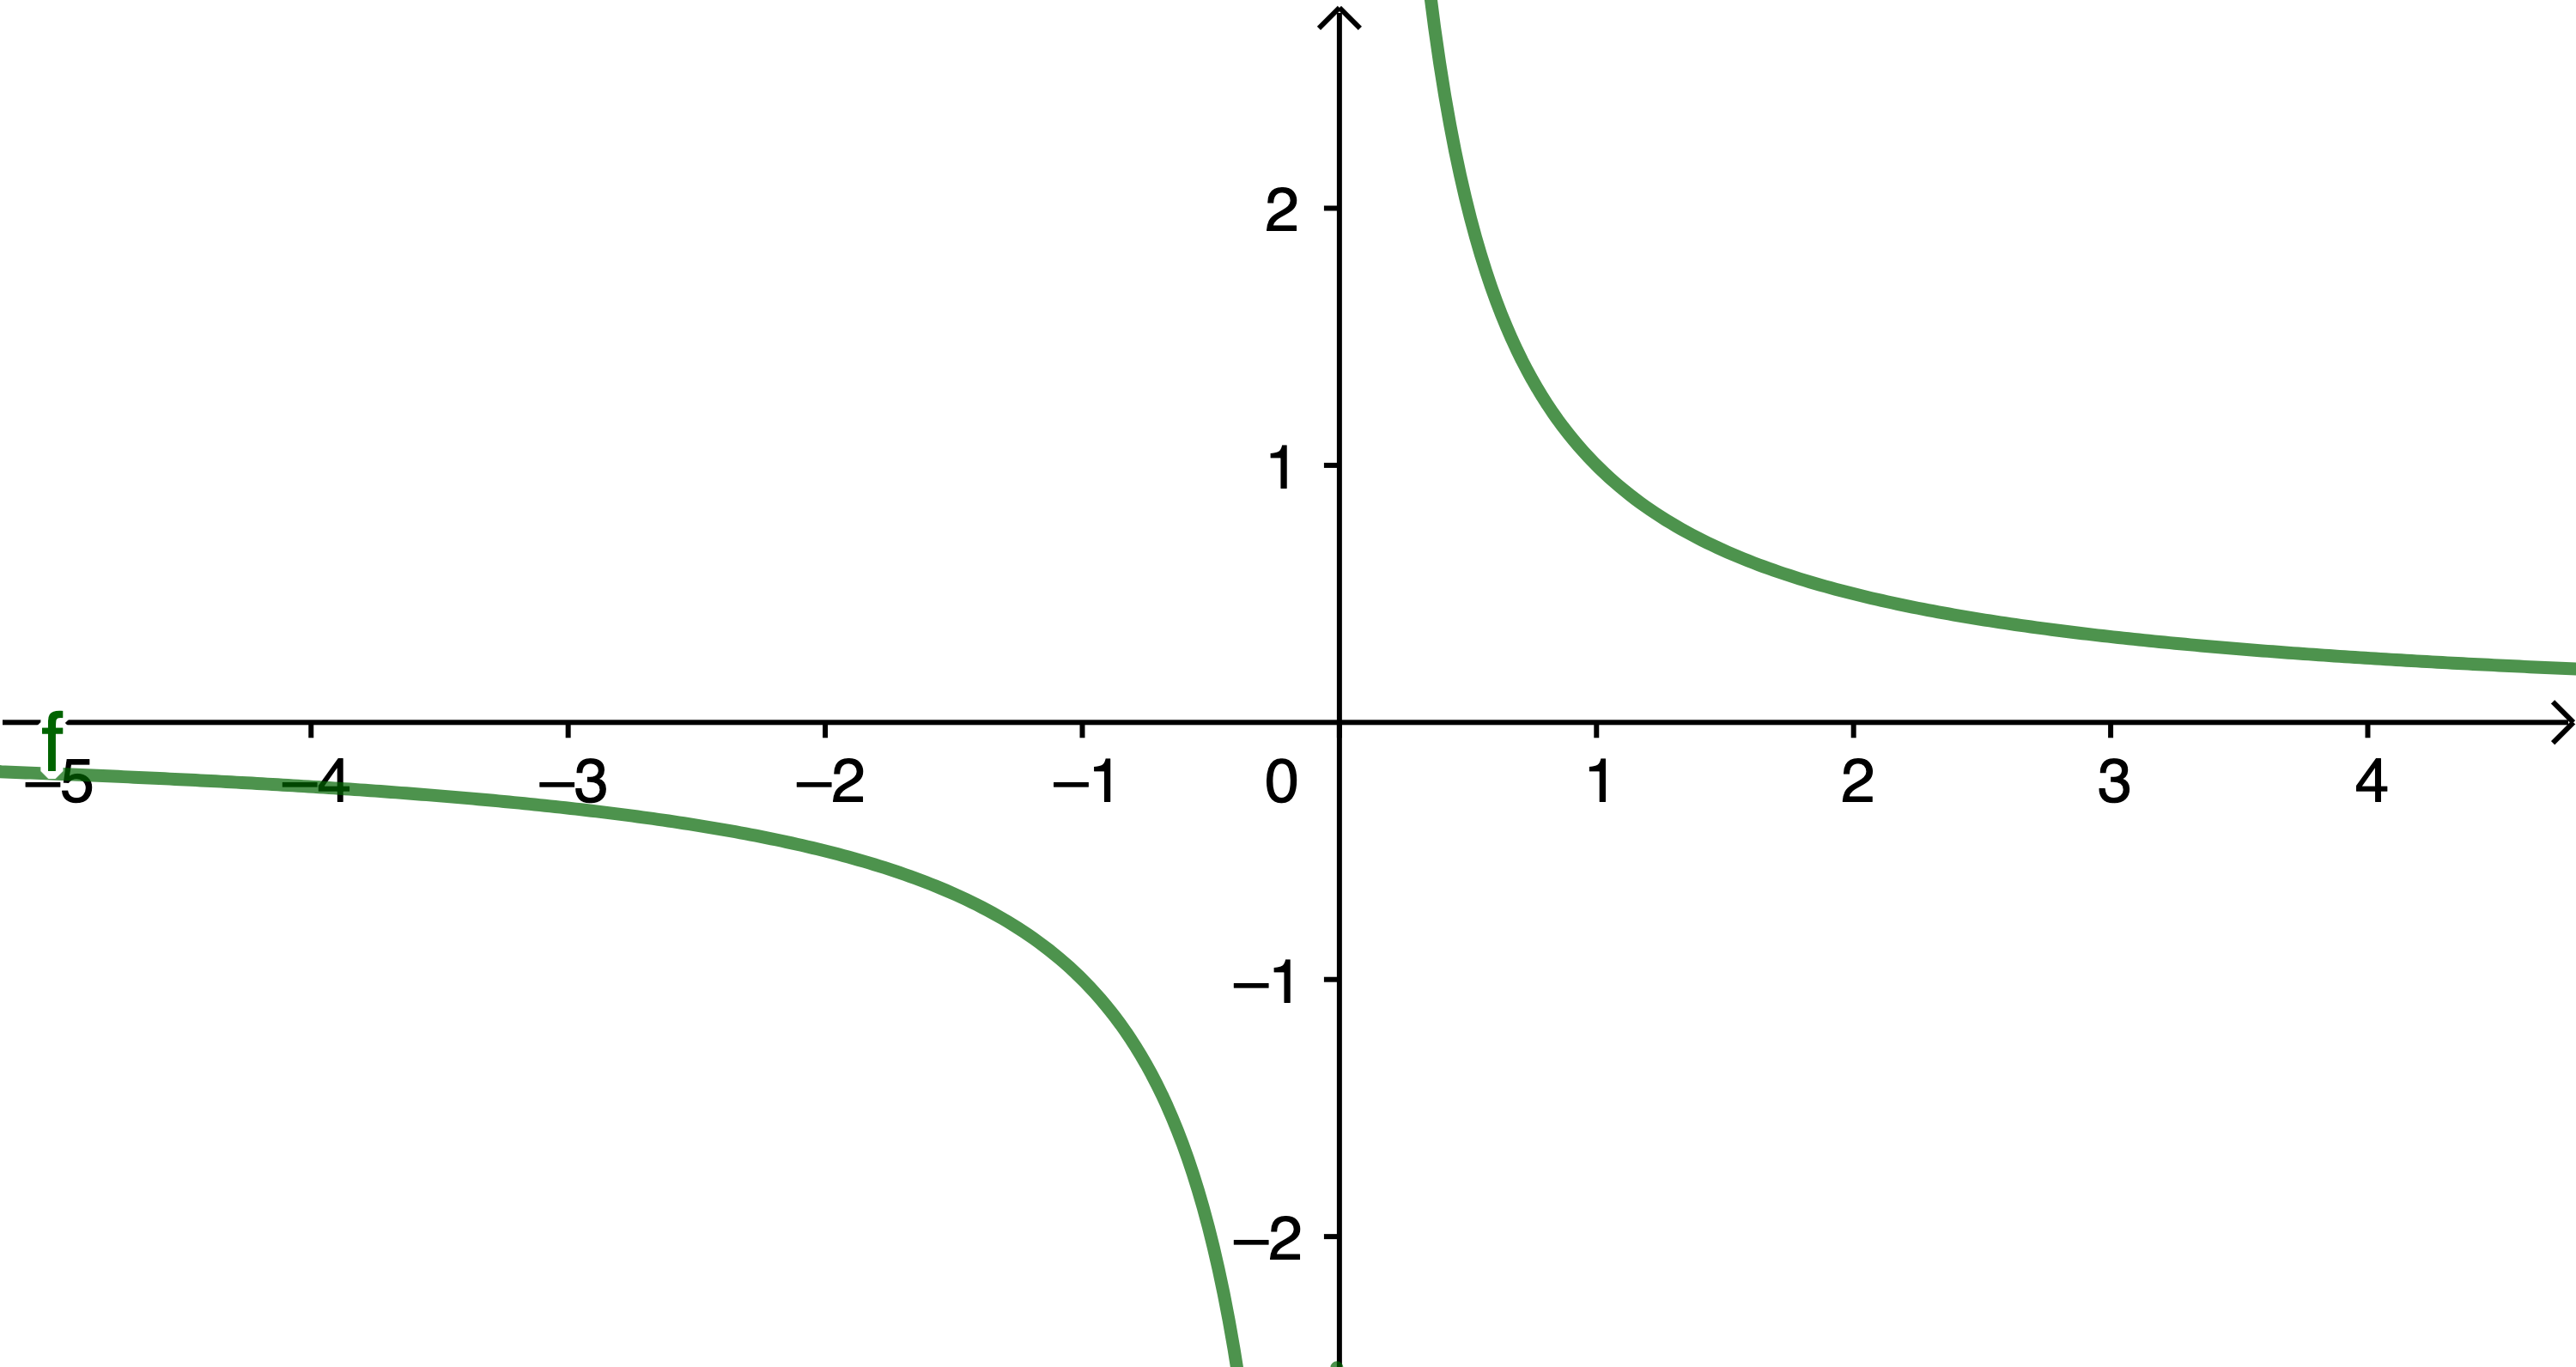
\includegraphics[scale=0.8]{media/kehrwert.png}
    \end{center}
    \end{enumerate}
     
\end{bsp}




\begin{ueb}{}{}
\begin{enumerate}
    \item Bestimme den links- und den rechtsseitigen Grenzwert der Funktion an der angegebenen Stelle. Ist die Funktion an dieser Stelle stetig?

    Bemerkung: Die Funktion $\lfloor x \rfloor$ ist die Abrundungsfunktion. Der Output ist die grösste ganze Zahl, die kleiner oder gleich $x$ ist.
    \begin{enumerate}
        \item $f(x)=x^2+x, \, a=3$
        \item  $f(x)=\lfloor x \rfloor, \, a=5$
        \item  $f(x)=\lfloor x-1 \rfloor, \, a=\frac{5}{2}$
        \item  $f(x)=\lvert x-5 \rvert, \, a=5$
        \item  $f(x)=\mathrm{sgn}(x-3), \, a=3$
        \item  $f(x)=\lfloor \cos(x)\rfloor, \, a=0$
    \end{enumerate}
    \item Gegeben ist die Funktion $f(x) = \left\{\begin{array}{ll}
        3-x, & x<2 \\\frac{x}{2}+1, &x\ge 2        
    \end{array}\right.$
    \begin{enumerate}
        \item Bestimme $\lim_{x\uparrow 4} f(x)$ und $\lim_{x\downarrow 4} f(x)$. Existiert $\lim_{x\to 4} f(x)$  ?
        \item Bestimme $\lim_{x\uparrow 2} f(x)$ und $\lim_{x\downarrow 2} f(x)$. Existiert $\lim_{x\to 2} f(x)$  ?
    \end{enumerate}
\end{enumerate}
\end{ueb}

\clearpage
\emph{Lösungen}
\begin{enumerate}
    \item Bestimme den links- und den rechtsseitigen Grenzwert der Funktion an der angegebenen Stelle. Ist die Funktion an dieser Stelle stetig?
    
    \begin{enumerate}
        \item $\lim\limits_{x \to 3^-} f(x) = 12$, \quad $\lim\limits_{x \to 3^+} f(x) = 12$ \newline $\Rightarrow$ Stetig
        \item $\lim\limits_{x \to 5^-} f(x) = 4$, \quad $\lim\limits_{x \to 5^+} f(x) = 5$ \newline $\Rightarrow$ Nicht stetig
        \item $\lim\limits_{x \to \frac{5}{2}^-} f(x) = 1$, \quad $\lim\limits_{x \to \frac{5}{2}^+} f(x) = 1$ \newline $\Rightarrow$  Stetig
        \item $\lim\limits_{x \to 5^-} f(x) = 0$, \quad $\lim\limits_{x \to 5^+} f(x) = 0$ \newline $\Rightarrow$ Stetig
        \item $\lim\limits_{x \to 3^-} f(x) = -1$, \quad $\lim\limits_{x \to 3^+} f(x) = 1$ \newline $\Rightarrow$ Nicht stetig
        \item $\lim\limits_{x \to 0^-} f(x) = 0$, \quad $\lim\limits_{x \to 0^+} f(x) = 0$ aber $\cos(0)=1$ \newline $\Rightarrow$ Nicht stetig
    \end{enumerate}
    
    \item Gegeben ist die Funktion 
    \[
        f(x) = \begin{cases} 
        3-x, & x<2 \\ 
        \frac{x}{2}+1, & x\geq 2 
        \end{cases}
    \]
    \begin{enumerate}
        \item $\lim\limits_{x \uparrow 4} f(x) = 3$, \quad $\lim\limits_{x \downarrow 4} f(x) = 3$ \newline $\Rightarrow$ Existiert mit Wert $3$
        \item $\lim\limits_{x \uparrow 2} f(x) = 1$, \quad $\lim\limits_{x \downarrow 2} f(x) = 2$ \newline $\Rightarrow$ Grenzwert existiert nicht
    \end{enumerate}
\end{enumerate}

\clearpage
Bei einer `asymptotischen Analyse' werden die Grenzwerte einer Funktion für $x\to\pm\infty$ und an allen Definitionslücken bestimmt. Damit kann man sich eine gute Vorstellung des Funktionsgraphen machen.

\begin{bsp}
    {Asymptotische Analyse der Funktion $f(x)= \frac{x^2-4}{x^2-5x+6}$}{}
    
    \vspace*{19cm}
\end{bsp}

\begin{ueb}
    {}{}
    Führe die asymptotische Analyse durch.
    \begin{enumerate}
        \item $f(x) = \frac{x^2-2x-3}{x^2-9}$
        \item $g(x) = \frac{x}{x^3-4x^2+4x}$
    \end{enumerate}

    Zeichne die entsprechenden Graphen mit Geogebra, um die Lösung zu überprüfen. 
\end{ueb}
\clearpage
\section{Differentialrechnung}
\subsection{Einleitung}
\begin{LA}
    {Weg-Zeit-Diagramme}{}
    Eine Rangierlokomotive bewegt sich entlang der Geleise vor- und rückwärts. 
    \begin{center}
        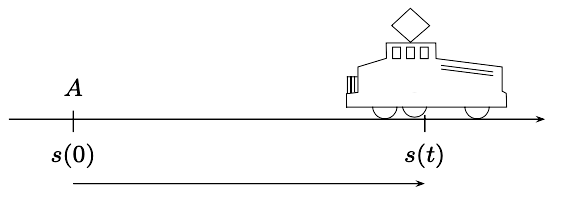
\includegraphics[width=0.25\textwidth]{media/rangierlok.png}
        
    \end{center}
    
    Das folgende „Weg-Zeit-Diagramm“ beschreibt die Bewegung der Lokomotive während 2 Minuten. 
    Auf der horizontalen Achse ist die Zeit in Sekunden dargestellt. Auf der vertikalen Achse ist der Abstand in Metern von einem Bezugspunkt A auf den Geleisen angegeben. Der Zeitpunkt $t=0$ ist der Moment, in welchem die Lok den Punkt A passiert.
    \begin{center}
        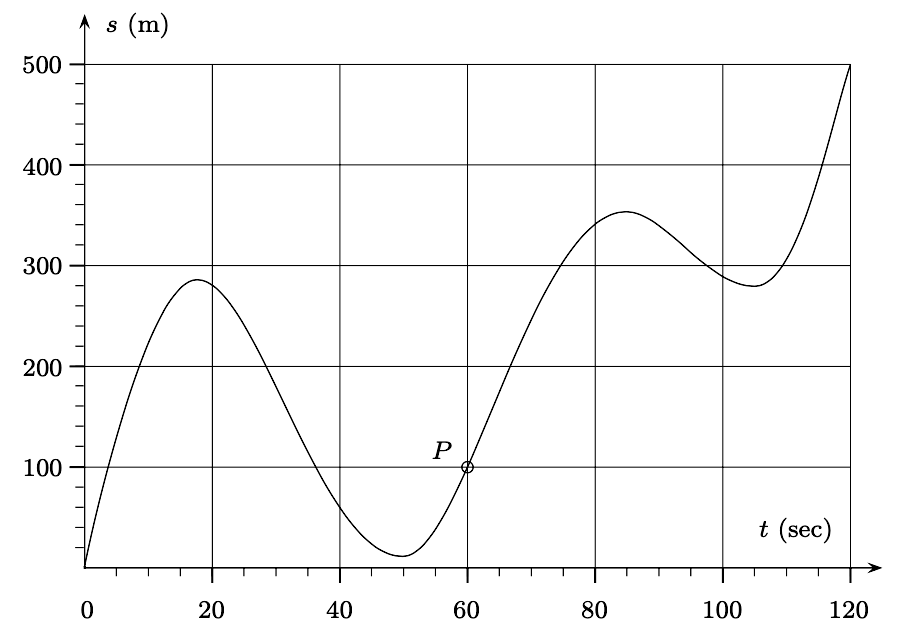
\includegraphics[width=0.6\textwidth]{media/LokWegZeit.png}
    \end{center}
    \begin{enumerate}
        \item Zu welchen Zeitpunkten befindet sich die Lok 200 Meter vom Punkt A entfernt?
        \item In welchen Zeitintervallen fährt die Lok rückwärts?
        \item Nach 60 Sekunden ist die Lok ungefähr 100m vom Punkt A entfernt. Wie viele Meter ungefähr hat sie \textbf{insgesamt} zurückgelegt?
        \item Berechne ungefähr die durchschnittliche Geschwindigkeit der Lok während den ersten 10 Sekunden.
        \item Berechne ungefähr $\frac{s(40)-s(20)}{40-20}$. Was für eine physikalische Bedeutung hat das Resultat und wieso ist es negativ?
        \item Schätze: Wann fährt die Lok am langsamsten? Wann am schnellsten?
    \end{enumerate}

\end{LA}
\clearpage
\begin{LA}
    {Mittlere und momentane Geschwindigkeit}{}
    Auf der 100-Meter-Bahn der KS Im Lee wird ein Roboter getestet. Er wird auf die Startlinie gesetzt und beschleunigt schnell in Richtung Ziellinie. Während der Fahrt folgt die Bewegung des Roboters der Bewegungsgleichung:
\[
    s(t) = \frac{1}{4} t^2
\]
Das bedeutet, dass der Roboter nach $t$ Sekunden die Strecke $s(t) = \frac{1}{4} t^2$ in Metern zurückgelegt hat. Wir denken uns entlang der Bahn ein Messband ausgelegt, sodass wir immer die Position des Roboters in Metern nach dem Startpunkt ablesen können.
\begin{enumerate}
    \item Skizziere den Graphen der Funktion $s(t)$ im Bereich $0 \leq t \leq 8$.

 

\begin{center}
    \begin{tikzpicture}
       
        
        % Rasterlinien
        % \draw[gray!30, step=1] (0,0) grid (8,9);
        \draw[gray!30,xstep=1, ystep=0.5] (0,0) grid (9,9);  % X-Richtung (Schrittweite 1)
        %\draw[gray!30,step=0.5,ystep=0.5] (0,0) grid (9,9);  % Y-Richtung (Schrittweite 0.5)
         % Achsen
         \draw[->, thick] (0,0) -- (9,0) node[right] {$t$ (Sek)};
         \draw[->, thick] (0,0) -- (0,9) node[above] {$s$ (m)};
        
        % Beschriftungen der Achsen
        \foreach \x in {0,1,2,3,4,5,6,7,8} {
            \node[below] at (\x,0) {\x };
        }
        \foreach \y in {0,1,2,3,4,5,6,7,8,9,10,11,12,13,14,15,16,17} {
            \node[left] at (0,\y/2) {\y };
        }
    \end{tikzpicture}
\end{center}


    \item Welche Position lesen wir auf dem Messband 2 Sekunden nach dem Start ab? Und welche Position 6 Sekunden nach dem Start? Markiere die entsprechenden Punkte auf dem Graphen.
    \item Welche Distanz legt der Roboter zwischen dem Zeitpunkt $t=2$ und $t=6$ zurück? Wie gross ist demnach die Durchschnittsgeschwindigkeit $\bar{v}$ in m/s zwischen den beiden genannten Zeitpunkten?
    \item Zur Berechnung von $\bar{v}$ haben wir so etwas wie „obsi/vorwärts“ gerechnet. Von welcher Geraden ist $\bar{v}$ die Steigung? Zeichne die Gerade in den Graphen oben ein.
    \item Berechne die Durchschnittsgeschwindigkeit des Roboters zwischen den Zeitpunkten $t=2$ und $t=2+\Delta t$ für $\Delta t=4,3,2,1,0.5$.
    \begin{center}
        \begin{tabular}{p{1.5cm} p{1.5cm} p{1.5cm} p{1.5cm} p{1.5cm} p{1.5cm}}
            \hline
            $\Delta t$ & 4 & 3 & 2 & 1 & 0.5 \\
            \hline
            $\bar{v}$ &  &  & &  &  \\
            \hline
                
        \end{tabular}
    \end{center}
  

    \item Bisher war immer die Rede von einer durchschnittlichen Geschwindigkeit im Intervall $[2,2+\Delta t]$. Wie schnell aber fährt der Roboter genau zum Zeitpunkt $t=2$? Das heisst, schätze seine Momentangeschwindigkeit $v(2)$.
    \item Von welcher Geraden ist $v(2)$ die Steigung? Zeichne die Gerade in den Graphen oben.
    \item Was ist die Momentangeschwindigkeit des Roboters zum Zeitpunkt $t=8$?
\end{enumerate}



\end{LA}

\begin{LA}
    {Temperaturverlauf im Ofen}{}
    Während den zehn Minuten, in denen ein Ofen auf 200°C erhitzt wird, verläuft die Temperatur nach der Gleichung:
\[
    T(t) = -\frac{9}{5} (t-10)^2 + 200
\]
wobei $t$ die Zeit in Minuten und $T$ die Temperatur in °C angibt.

\begin{center}
    \begin{tikzpicture}[scale=0.8]
        \begin{axis}[
            width=12cm, height=8cm,
            grid=major,
            xlabel={$t$ (Minuten)},
            ylabel={$T$ (°C)},
            xmin=0, xmax=10,
            ymin=0, ymax=200,
            xtick={0,1,2,3,4,5,6,7,8,9,10},
            ytick={0,25,50,75,100,125,150,175,200},
            domain=0:10,
            samples=100,
            thick,
            smooth,
            axis lines=middle,
            axis line style={->},
            enlargelimits=false,
            clip=false,
            tick align=outside
        ]
        \addplot[red, thick] {-9/5*(x-10)^2 + 200};
        \end{axis}
    \end{tikzpicture}
\end{center}
\begin{enumerate}
    \item Berechne die Steigung der Sekante, welche den Graphen von $T$ an den Stellen $t_1=5$ und $t_2=7$ schneidet.
    \item Was hat das Resultat aus 1. für eine Einheit? Was für eine Bedeutung hat es in Bezug auf den Ofen?
    \item \textbf{Challenge:} Gib einen Term in Abhängigkeit von $\Delta t$ an, mit dem man die Steigung der Sekante berechnen kann, die den Graphen von $T$ an den Stellen $t_1=5$ und $t_2=5+\Delta t$ schneidet.
    \item \textbf{Challenge:} Was passiert, wenn $\Delta t$ immer kleiner wird ($\Delta t \to 0$)? Was für eine geometrische und physikalische Bedeutung hat der Grenzwert?
\end{enumerate}

\end{LA}



























\clearpage
\subsection{Differenzenquotient und Differentialquotient}
Die Lernaufgaben zu Beginn des Abschnittes beschreiben gänzlich unterschiedliche Situationen. Die Rechenschritte, die zur Antwort auf die gestellten Fragen geführt haben, weisen aber enorme Parallelen auf. Damit wir diese Gemeinsamkeiten unabhängig vom gewählten Kontext hervorheben können, werden wir sie im Folgenden an einer generischen Funktion $f$ beschreiben.
 Betrachten wir also eine Funktion $f$, die auf einem Intervall der reellen Zahlen definiert ist:


\begin{definition}
    {Differenzenquotient}{}
    Zu einer gegebenen Funktion und zwei verschiedenen Stellen $x_0$ und $x_0+\Delta x$ heisst der Term:
\[
    \frac{f(x_0+\Delta x)-f(x_0 )}{\Delta x}
\]
Differenzenquotient.

Er gibt die Steigung der Sekante durch die Punkte \((x_0, f(x_0))\) und \((x_0+\Delta x, f(x_0+\Delta x))\) an.

\begin{center}
    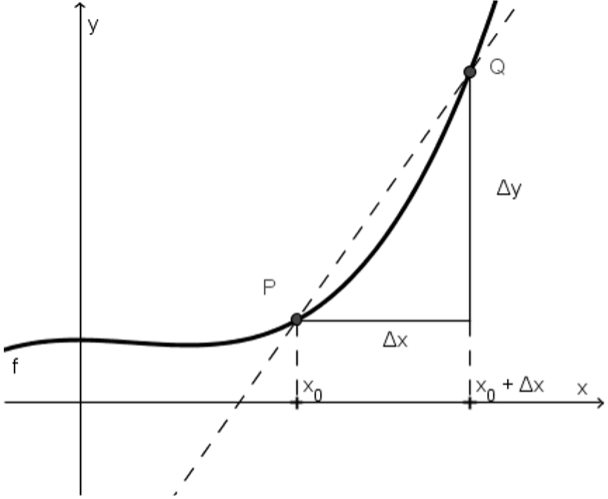
\includegraphics[width = 0.5 \textwidth]{media/differenzenquo.png}
 \end{center}


Häufig wird statt $\Delta x$ auch der Buchstabe $h$ (für horizontaler Abstand) verwendet. Der Differenzenquotient lautet dann:
\[
    \frac{f(x_0+h)-f(x_0 )}{h}
\]


\end{definition}

Je nach Anwendung kann der Differenzenquotient die \emph{durchschnittliche} Geschwindigkeit einer Sprinterin, die \emph{durchschnittliche} Beschleunigung einer Rakete oder die \emph{durchschnittliche} Abnahmerate der Wirkstoffkonzentration pro Zeiteinheit eines Medikaments darstellen.

Ist man an der \emph{momentanen} Geschwindigkeit, Beschleunigung oder Änderungsrate interessiert, bedient man sich einer Methode, die wir in den Einführungsaufgaben mehrfach angewendet haben: Wir lassen $\Delta x$ bzw. $h$ immer kleiner werden und untersuchen das Grenzverhalten des Differenzenquotienten für $\Delta x\to 0$ bzw. $h\to 0$.

\begin{definition}{Differentialquotient}{}
    Falls der Grenzwert
    \[
    \lim\limits_{h\to 0} \frac{f(x_0+h)-f(x_0 )}{h}
    \]
    existiert, so nennt man ihn Differentialquotient oder (erste) Ableitung der Funktion an der Stelle $x_0$. 
    \begin{center}
        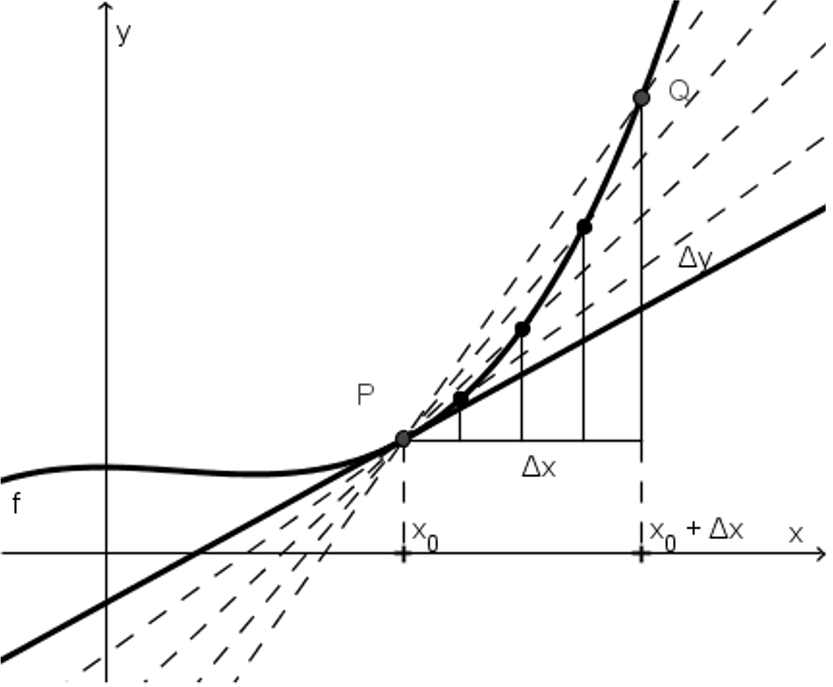
\includegraphics[width = 0.5 \textwidth]{media/differentialquo.png}
     \end{center}
    
    Bezeichnungen:
    \[
        f'(x_0) \quad \text{oder} \quad \frac{d}{dx} f(x_0)
    \]
    Gesprochen: „$f$ Strich von $x_0$“ oder „$df$ nach $dx$ an der Stelle $x_0$“.
    
    Die Ableitung der Funktion an der Stelle $x_0$ entspricht der Steigung der Tangente an den Graphen im Punkt $ (x_0, f(x_0)) $.  
    
    
    
\end{definition}


\begin{bsp}
    {Berechnung des Differentialquotienten}{}
    Gegeben sei die Funktion $f(x)=\frac{1}{2}x^2-x$. Gesucht ist die Ableitung von $f$ an der Stelle $x_0=5$

    \vspace*{6.5cm}

    % Als erstes bestimmen wir den Differenzenquotienten:
    % \begin{align*}
    %    \frac{\Delta y}{\Delta x} &= \frac{f(5+h)-f(5)}{h} \\
    %    &= \frac{\left(\frac{1}{2} (5+h)^2-(5+h) \right) - \left(\frac{1}{2}5^2 -5 \right)}{h} \\
    %    %&= \frac{\left(\frac{1}{2}(25+10h+h^2)\right)-\frac{15}{2}}{h} //
    %    &= \frac{\frac{1}{2}h^2+4h}{h}
    % \end{align*}
    % Anschliessend bilden wir den Grenzwert für $h\rightarrow0$:
    % $$f'(5) = \lim_{h\rightarrow0}\frac{\Delta y}{\Delta x}= \lim_{h\rightarrow0} \frac{\frac{1}{2}h^2+4h}{h} = \lim_{h\rightarrow0}\left(\frac{1}{2}h+4\right) = 4$$
\end{bsp}


\begin{ueb}
    {}{}
    \begin{enumerate}
        \item Skizziere den Graphen der Funktion \( f(x) = 2x^2 \). Beantworte dann die folgenden Fragen mit einer Rechnung:
        \begin{enumerate}
          \item  Welche Steigung hat die Sekante, welche den Graphen an den Stellen \( x = 1 \) und \( x = 2 \) schneidet?
          \item Welche Steigung hat die Sekante, welche den Graphen an den Stellen \( x = 1 \) und \( x = 1 + h \) schneidet?
          \item Welche Steigung hat die Tangente, die den Graphen an der Stelle \( x = 1 \) berührt?
          \item Welche Steigung hat jene Tangente, die den Graphen an der Stelle \( x = 2 \) berührt?
        \end{enumerate}
      
        \item Sei \( f(x) = x^3 \).
       Berechne \( f'(2) \).
      
        \item Skizziere den Graphen der Funktion \( f(x) = x^2 - 5 \).
        \begin{enumerate}
          \item Berechne \( f'(0) \). Welche Eigenschaft des Graphen wird durch das Resultat verdeutlicht?
          \item Berechne \( f'(2) \). 
          \item Bestimme \( f'(-2) \). Entweder mit dem Differentialquotient oder indem du eine Eigenschaft der Parabel verwendest\dots
        \end{enumerate}
      
        \item Zeichne den Graphen der Funktion \( f(x) = \frac{1}{3}x - 1 \).\\
              Entscheide ohne zu rechnen: Wie gross sind \( \frac{d}{dx} f(1) \), \( \frac{d}{dx} f(2) \) und \( \frac{d}{dx} f(-42) \)?
        
        \item Die Funktion $N(t)$ beschreibt die Anzahl Bakterien einer Bakterienkultur $t$ Tage nach Beginn des Experiments. Beschreibe die Bedeutung der folgenden Grössen und geben deren Einheit an.
        \begin{enumerate}
            \item $N(10)-N(5)$
            \item $\frac{N(10)-N(5)}{5}$
            \item $\lim\limits_{h\to0}\frac{N(5+h)-N(5)}{h}$
        \end{enumerate}

        \item Ein Teilchen bewegt sich mit der Geschwindigkeit $v(t) = 2t^2 - 5t + 1$ [m/s] in Abhängigkeit von der Zeit $t$ [s]. Berechne die momentane Beschleunigung des Teilchens zum Zeitpunkt $t=1$.
        
        Bestimmen Sie auch die momentane Geschwindigkeit zur Zeit $t=1$ und beschreiben Sie die Bewegung des Teilchens zu diesem Zeitpunkt.
      
        \item \textbf{Achtung Doppelbrüche!}\\
        Sei \( f(x) = \frac{1}{x + 1} \). Berechne \( f'(1) \).
    
      \end{enumerate}
\end{ueb}

\clearpage
\emph{Lösungen:}


\begin{enumerate}
  \item
  \begin{enumerate}
    \item \( 6 \)
    \item \( 4 + 2h \)
    \item \( 4 \)
    \item \( 8 \)
  \end{enumerate}

  \item
   \( 12 \)
  

  \item
  \begin{enumerate}
    \item \( f'(0) = 0 \)
    \item \( f'(2) = 4 \)
    \item  \( f'(-2) = -4 \)
  \end{enumerate}

  \item
  \[
  \frac{d}{dx}f(1) = \frac{1}{3}, \quad
  \frac{d}{dx}f(2) = \frac{1}{3}, \quad
  \frac{d}{dx}f(-42) = \frac{1}{3}
  \]
  \item 
        \begin{enumerate}
            \item Bevölkerungszuwachs in Anzahl Bakterien.
            \item \emph{Durchschnittliche} Wachstumsrate der Population zwischen dem 5 und 10 Tag in Bakterien/Tag.
            \item  \emph{Momentane} Wachstumsrate der Population am fünften Tag in Bakterien/Tag.
        \end{enumerate}
\item Beschleunigung des Teilchens am Zeitpunkt \( t=1 \):
\[
    a(1) = v'(1) = -1
\]
Ausserdem gilt $v(1)=-2$. Bezüglich der ausgelegten Skala, welche die Position des Teilchens beschreibt, bewegt sich das Teilchen so, dass die Werte abnehmen. Wegen der negativen Beschleunigung, bewegt sich das Teilchen immer schneller in negativer Richtung.
  \item
   \( f'(1) = -\frac{1}{4} \)
  
\end{enumerate}
























\clearpage
\subsection{Ableitungsfunktion}




Nach den Erkenntnissen aus dem Kapitel über Grenzwerte wissen wir, dass diese nicht immer existieren. Somit kann es auch sein, dass für eine gegebene Funktion den Differentialquotienten an einer bestimmten Stelle gar nicht gebildet werden kann.
\begin{definition}
    {Differenzierbarkeit}{}
    Sei $f$ eine beliebige Funktion und $x_0 \in \mathbb{D}_f$. Falls der Grenzwert 
    $$ \lim_{h\rightarrow0}\frac{f(x_0+h)-f(x_0)}{h} $$
    existiert, so sagt man, dass die Funktion $f$ an der Stelle $x_0$ \emph{differenzierbar} ist.
\end{definition}

Die Betragsfunktion $x\mapsto |x|$ ist beispielsweise überall differenzierbar mit Ausnahme der Stelle $x_0=0$.

\begin{center}
    \begin{tikzpicture}
        \begin{axis}[
            width=10cm, height=6cm,
            grid=major,
            xlabel={$x$},
            ylabel={$y$},
            xmin=-5, xmax=5,
            ymin=-1, ymax=5,
            xtick={  -4, -3, -2, -1, 0,1,2,3,4},
            ytick={0,1,2,3,4},
            domain=-5:5,
            samples=500,
            thick,
            smooth,
            axis lines=middle,
            axis line style={->},
            enlargelimits=false,
            clip=false,
            tick align=outside
        ]
        \addplot[red, thick] {abs(x)};
        \end{axis}
    \end{tikzpicture}
\end{center}


% \begin{center}
%     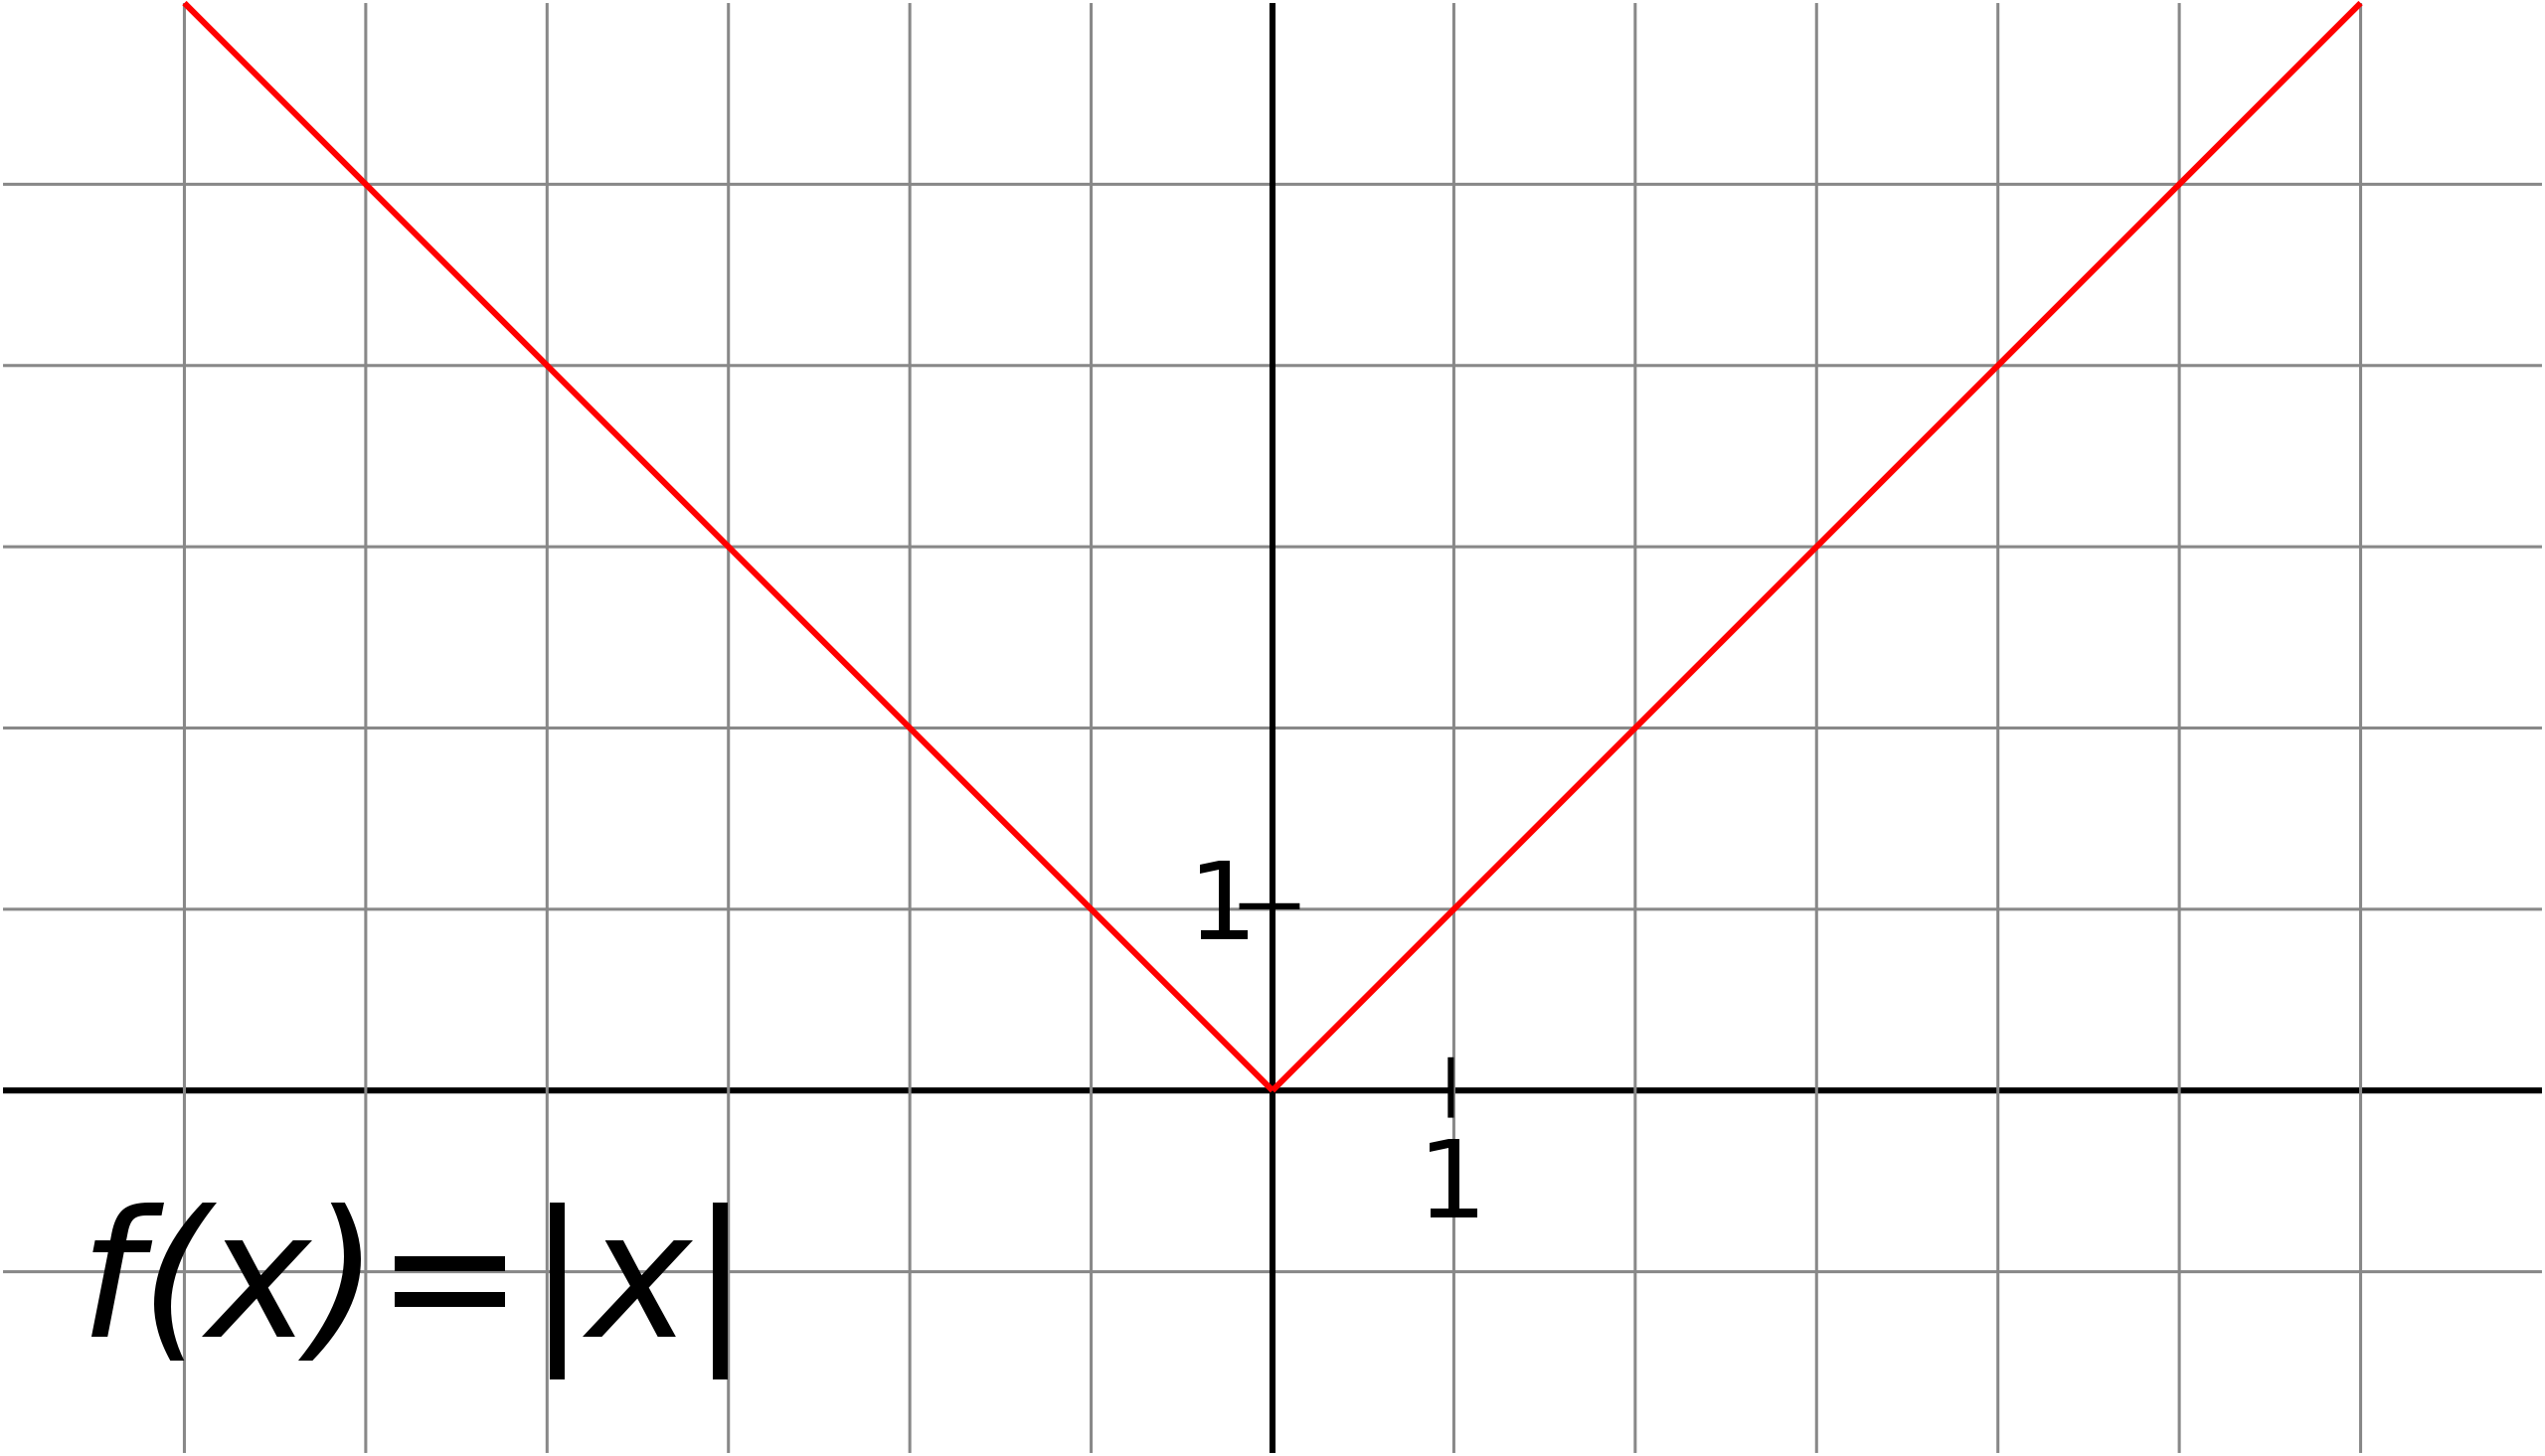
\includegraphics[scale=0.1]{media/Abs(x).png}
% \end{center}
Was wären in diesem Fall der links- bzw. rechtsseitige Grenzwert $\lim\limits_{h\nearrow 0} \frac{f(0+h)-f(0)}{h}$ und $\lim\limits_{h\searrow 0} \frac{f(0+h)-f(0)}{h}$?

Wenn die Funktion überall differenzierbar ist, kann in jedem Punkt des Graphen die Steigung der Tangente ermittelt werden. Die Zuordnung \emph{
$x\mapsto$ Steigung des Graphen von $f$ an der Stelle $x$} ist wieder eine Funktion!

\begin{definition}
    {Ableitungsfunktion}{}
    Gegeben sei eine differenzierbare Funktion $f$. Die Funktion mit der Zuordnungsvorschrift:
    $$x\mapsto f'(x)=\lim_{h\rightarrow0}\frac{f(x+h)-f(x)}{h}$$
    heisst die \emph{Ableitungsfunktion} (kurz: \emph{die Ableitung}) der Funktion $f$. Sie wird mit $f'$ bezeichnet. 
    \newline
    Geometrisch interpretiert beschreibt der Output von $f'$ die Steigung der Tangente an den Graphen von $f$ im Punkt $(x|f(x))$.
  
\end{definition}

Einen ungefähren Verlauf der Ableitungsfunktion kann man sich mit rein grafischen Überlegungen machen:
\begin{bsp}{Graph der Ableitungsfunktion}{}
    In der folgenden Abbildung ist der Graph einer Funktion $f$ dargestellt. Skizziere den ungefähren Verlauf des Graphen der Ableitungsfunktion $f'$.
    \begin{center}
        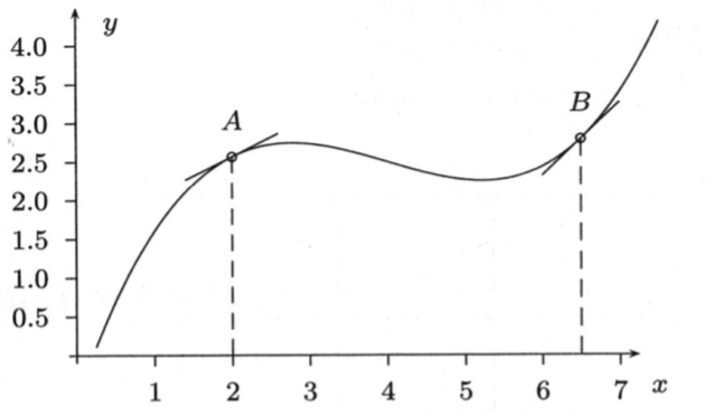
\includegraphics[scale = 1.2]{media/graphischesAbleiten.png}
    \end{center}
    \vspace{12
    cm}
\end{bsp}

\clearpage
\begin{ueb}
    {Graph der Ableitungsfunktion}{}
    \begin{enumerate}
        \item Die Grafiken I bis IV zeigen die ursprünglichen Graphen von vier Funktionen $f$, die Grafiken a) bis d) die Graphen der vier Ableitungsfunktionen $f'$. Welcher $f$-Graph gehört zu welchem $f'$-Graph?
        \begin{center}
            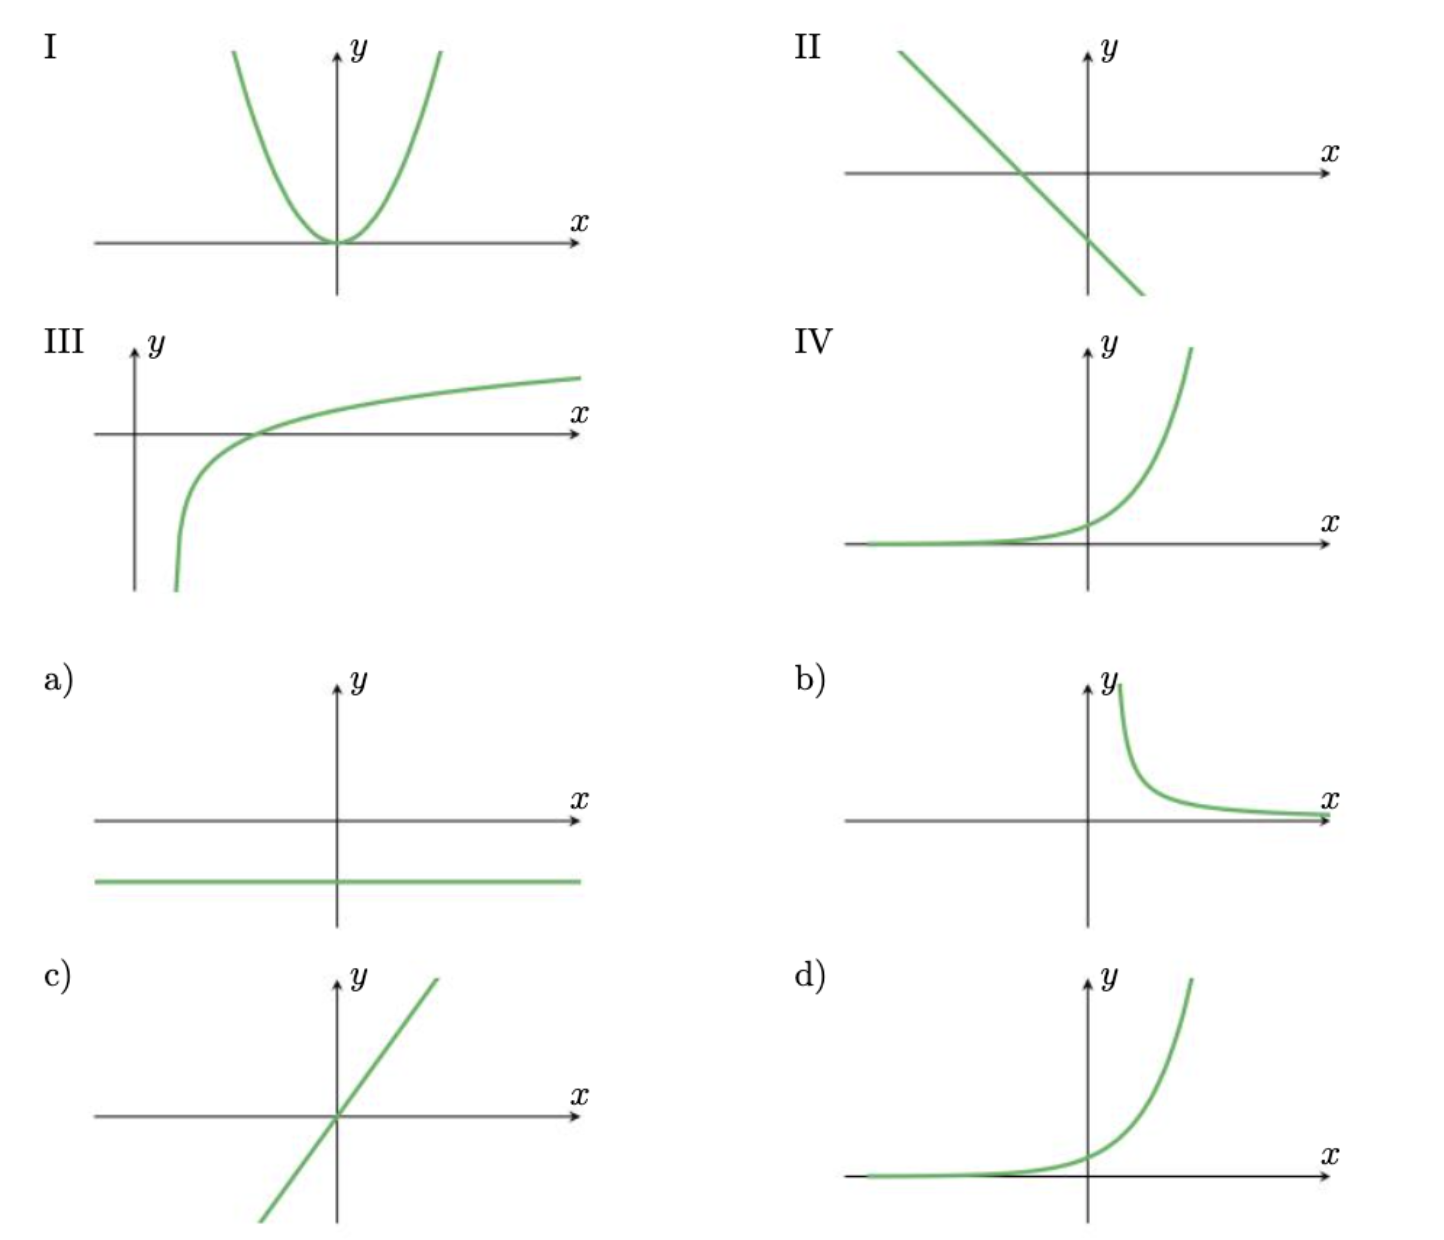
\includegraphics[width = 0.8 \textwidth]{media/zuordnungf-f.png}
        \end{center}
        \item Skizziere den Graphen der Ableitungsfunktion $f'$ der dargestellten Funktion $f$ in das gleiche Koordinatensystem.
        \begin{center}
            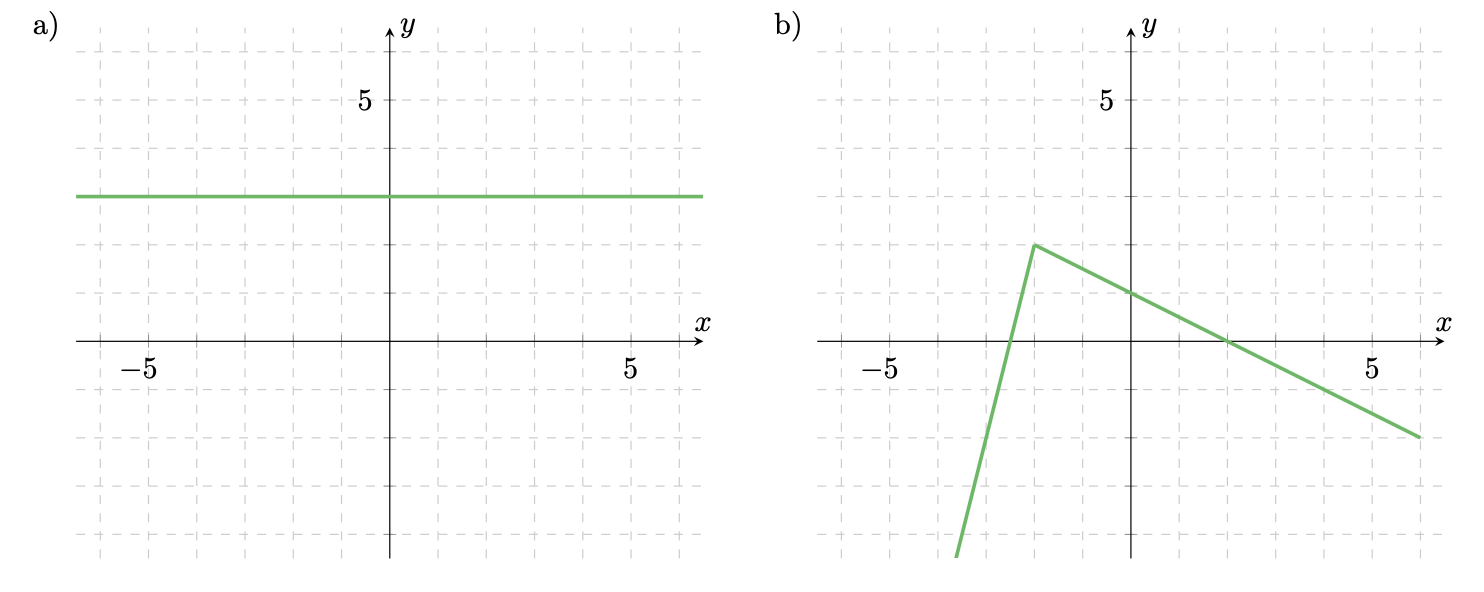
\includegraphics[width = 0.8 \textwidth]{media/graphischAbleiten1.png}
        \end{center}
        \pagebreak
        \item Skizziere den Graphen der Ableitungsfunktion $f'$ der dargestellten Funktion $f$ in das gleiche Koordinatensystem.
        \begin{center}
            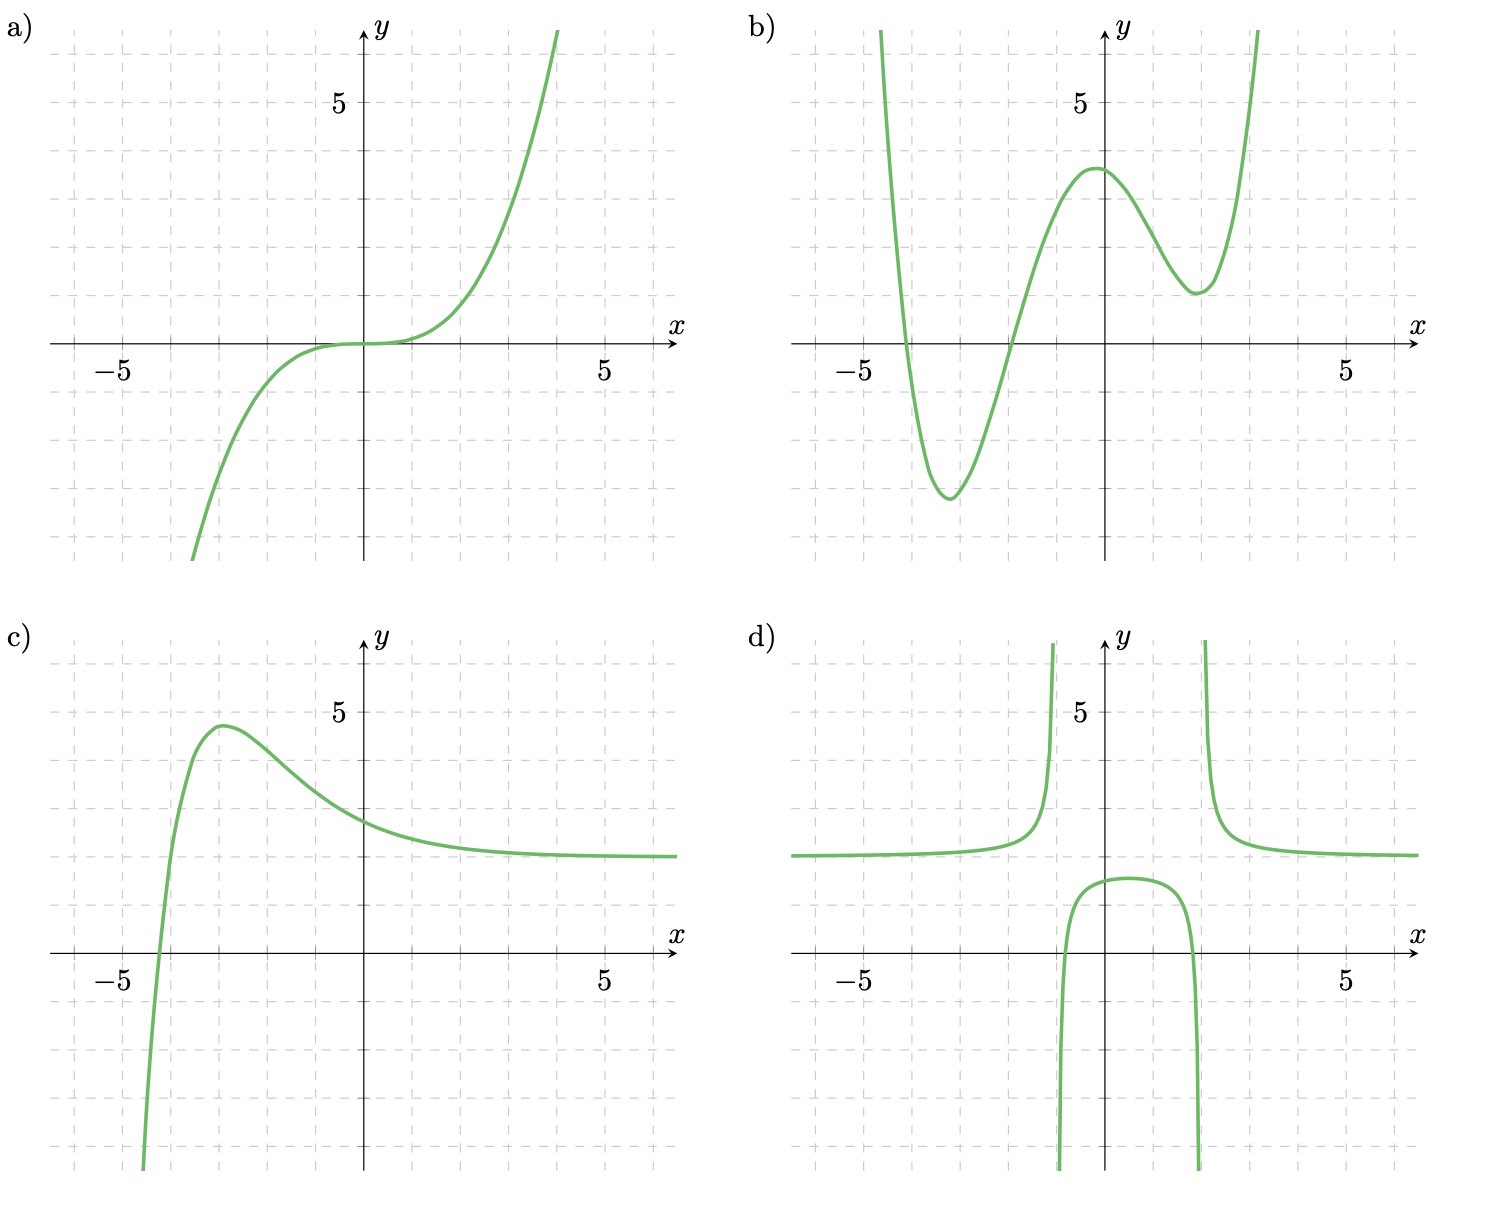
\includegraphics[width = 0.8 \textwidth]{media/GraphischAbleiten 2.png}
        \end{center}
    \end{enumerate}
\end{ueb}

\clearpage
\emph{Lösungen:}
\begin{enumerate}
    \item I-c), II-a), III-b), IV-d)
    \item Ableitungsgraphen
    
    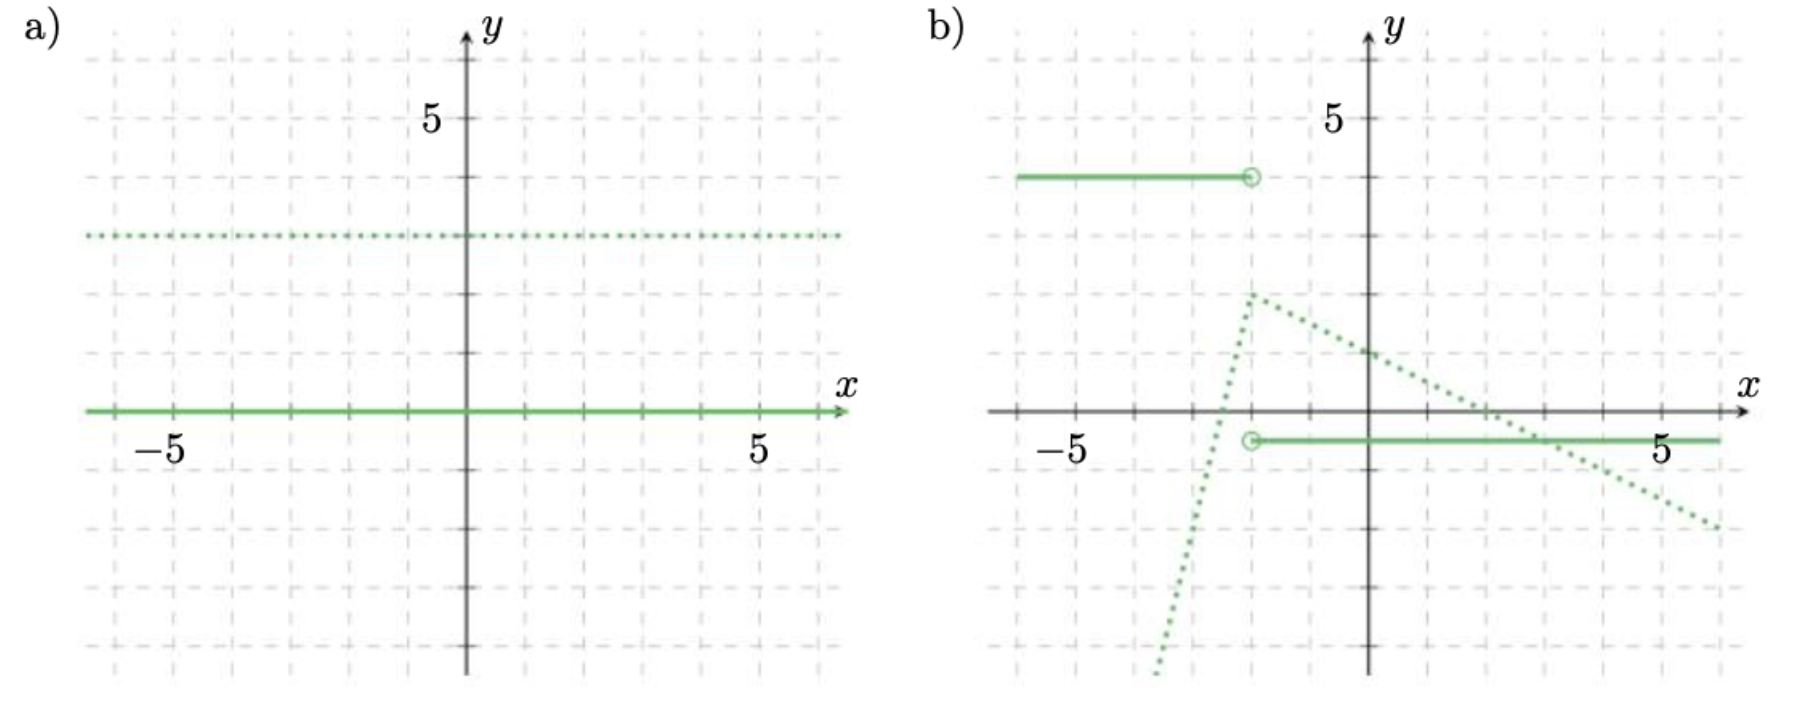
\includegraphics[width = 0.8 \textwidth]{media/lsgGraphischAbleiten1.png}
    
    \item Ableitungsgraphen
    
    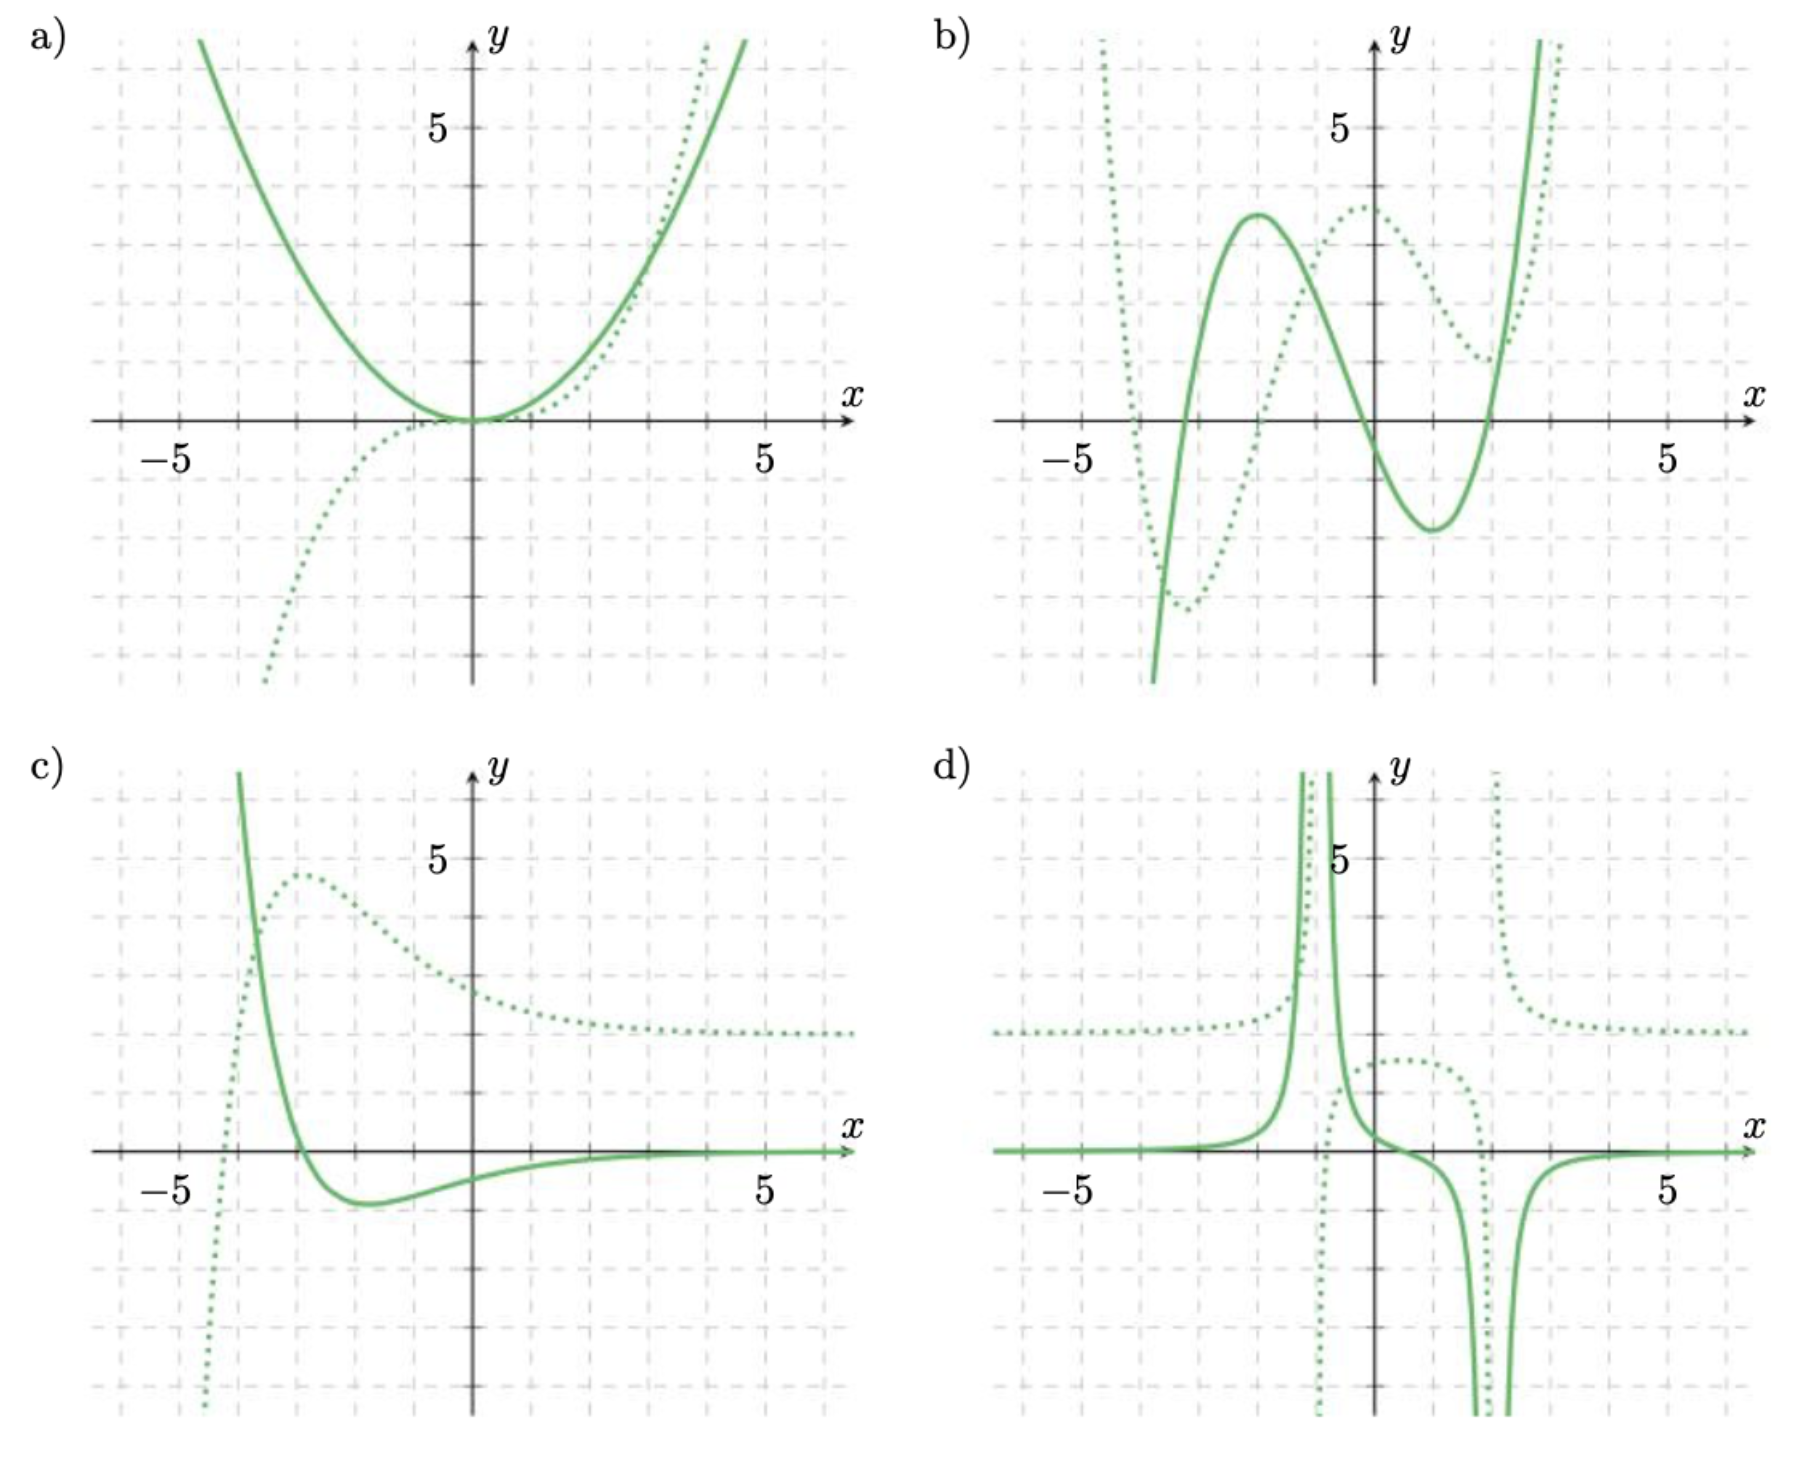
\includegraphics[width = 0.8 \textwidth]{media/LsgGraphischAbleiten2.png}

\end{enumerate}


















\clearpage
Häufig möchte man auch die Funktionsgleichung der Ableitung ermitteln, nicht nur den ungefähren Verlauf des Graphen. Dazu greift man wieder zum Differenzialquotienten. 
$$f'(x) = \lim_{h\to0}\frac{f(x+h)-f(x)}{h}$$

Betrachten wir dazu ein Beispiel:

\begin{bsp}
    {Berechnung der Ableitungsfunktion}{berechnenderAbleitung}
    Sei $f(x)=x^2+1$. Die Gleichung der Ableitungsfunktion kann wie folgt hergeleitet werden:

    \vspace*{15cm}
    % \begin{align*}
    %     f'(x)   &= \lim_{h\rightarrow0}\frac{f(x+h)-f(x)}{h}\\
    %             &=  \lim_{h\rightarrow0}\frac{\left((x+h)^2+1\right)-\left(x^2+1\right)}{h}\\
    %             &= \lim_{h\rightarrow0}\frac{\left(x^2+2hx+h^2+1\right)-\left(x^2+1\right)}{h}\\
    %             &= \lim_{h\rightarrow0}\frac{2hx+h^2}{h}\\
    %             &= \lim_{h\rightarrow0}\left(2x+h\right)\\
    %             &= 2x
    % \end{align*}
    % Die erste Ableitung von $f$ ist damit $f'(x)=2x$. In anderen Worten: Die Tangente, welche den Graphen von $y=x^2+1$ an der Stelle $x$ berührt hat die Steigung $2x$.
    % So hat die Tangente an $y=x^2+1$ an der Stelle $x=5$ die Steigung $f'(5)=10$.
    
\end{bsp}
\clearpage
Mit der Gleichung der Ableitungsfunktion lässt sich die Geradengleichung der Tangente an einen Funktionsgraphen bestimmen:

\begin{bsp}
    {Gleichung der Tangente}{}
    Sei wieder $f(x)=x^2+1$. Wie lautet die Gleichung der Tangente, welche den Graphen an der Stelle $x=5$ berührt?
    
    \vspace*{18cm}

\end{bsp}

\clearpage
\begin{ueb}
    {}{}
    \begin{enumerate}
        \item 
    Bestimme die Gleichung der Ableitungsfunktion \( f' \) der Funktion \( f  \).

            \begin{enumerate}
            \item \( f(x) = x^2 + 3 \). Vergleiche das Resultat mit \Cref{bsp:berechnenderAbleitung} und erkläre.
            \item \( f(x) = 2x^3 \). Verwende das Pascalsche Dreieck.
            \item \( f(x) = 3x \). Wieso ergibt das seltsame Resultat Sinn?
            \item \( f(x)= \dfrac{1}{x} \). Achtung Doppelbrüche!
            \item \( f(x) =\sqrt{x} \). Tipp: Erweitere den Differenzenquotienten mit $\sqrt{x+h} + \sqrt{x}$ 
            \end{enumerate}
    \item Bestimme die Gleichung der Tangente, welche die Funktion $f$ an der Stelle $x_0$ berührt. Verwende die Resultate aus Aufgabe 1.
    \begin{enumerate}
        \item \( f(x) = x^2 + 3, \qquad x_0  = -3 \). 
        \item \( f(x) = 2x^3 , \qquad x_0  = 1 \).
        \item \( f(x) = 3x , \qquad x_0  = 1 \). 
        \item \( f(x)= \dfrac{1}{x} , \qquad x_0  = 2 \). 
        \item \( f(x) =\sqrt{x}, \qquad x_0  = 4 \).
        \end{enumerate}
    % \item Bestimme die Gleichung der Tangente, welche die Funktion $f= x^2 - x$ an der Stelle $x_0=1$ berührt.
    \item Die Position eines Teilchens wird durch die Funktion $s(t) = (2-t)^2$ beschrieben. Bestimmen Sie die Funktion $v(t)$, welche die momentane Geschwindigkeit des Teilchens zum Zeitpunkt $t$ beschreibt.
\end{enumerate}
\end{ueb}

\pagebreak
\emph{Lösungen:}
\begin{enumerate}
    \item Ableitungsfunktionen:
    \begin{enumerate}
      \item \( f'(x) = 2x \)
      \item \( f'(x) = 6x^2 \)
      \item \( f'(x) = 3 \)
      \item \( f'(x) = -\dfrac{1}{x^2} \)
      \item \( f'(x) = \dfrac{1}{2\sqrt{x}} \)
    \end{enumerate}
  
    \item Tangentengleichungen:
    \begin{enumerate}
      \item \( y = -6x - 6 \)
      \item \( y = 6x - 4 \)
      \item \( y = 3x \)
      \item \( y = -\dfrac{1}{4}x + 1 \)
      \item \( y = \dfrac{1}{4}x +1\)
    \end{enumerate}
  
    % \item Tangente an \( f(x) = x^2 - x \) bei \( x_0 = 1 \):
    % \[
    % y = x - 1
    % \]
    \item $v(t) = 2t-4$ 
  \end{enumerate}


\clearpage

%% Dieser Teil war für 3h2024 %%
%%%%%%%%%%%%%%%%%%%%%%%%%%%%%%%%%%%
% \section{Differentialrechnung}
% \setcounter{subsection}{2} % Damit die Nummerierung dem Buch entspricht

% \begin{definition}
%     {Differentialquotient - Ableitung - momentane Änderungsrate}
%     {}
%     Falls der Grenzwert
% $$\lim_{h\rightarrow0}\frac{f(x_0+h)-f(x_0)}{h}$$
% existiert, so nennt man ihn \emph{Differenzialquotient oder (erste) Ableitung oder momentane (oder lokale) Änderungsrate der Funktion $f$ an der Stelle $x_0$}.

% Bezeichnungen:
% $$f'(x_0)   \text{ oder }  \frac{d}{dx} f(x_0)$$
% Gesprochen: \glqq $f$ strich von $x_0$\grqq{} oder \glqq $df$ nach $dx$ an der Stelle $x_0$\grqq{}.

% Geometrisch entspricht die Ableitung der Funktion an der Stelle $x_0$ der Steigung der Tangente, welche den Graphen von $f$ im Punkt $(x_0 | f(x_0))$ berührt.

% \begin{center}
%     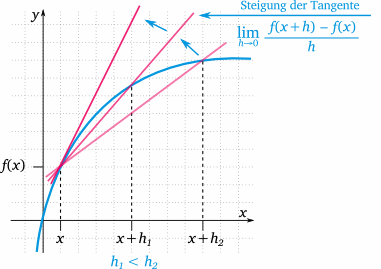
\includegraphics[scale = 0.5]{media/tangente02-3.png}
% \end{center} 

% \end{definition}
%%%%%%%%%%%%%%%%%%%%%%%%%%%%%%%%%%%%%%%%%%%%%%


\subsection{Erste Ableitungsregeln}
\grqq Es wäre wenig attraktiv, für jede Funktion, die uns begegnet, immer den Differenzialquotienten auszurechnen, um die Ableitung in Erfahrung zu bringen, zumal wir schon gesehen haben, dass dies zu erheblichen technischen Schwierigkeiten führen kann. Viel angenehmer wäre es, wir würden über einen überschaubaren Satz von Ableitungsregeln verfügen, die das Differenzieren aller relevanten Funktionstypen erleichtern. Zweifellos müssen wir zum Beweis dieser Regeln immer wieder den Differenzialquotienten benutzen. Sind die Regeln aber erst einmal gefunden, wird es sein, als wären wir über eine Leiter auf ein höheres Niveau gestiegen und könnten die Leiter nun, da wir oben angekommen sind, unter uns wegstossen. Wir werden sie – jedenfalls für den technischen Vorgang des Differenzierens – nicht mehr nötig haben. Darin liegt der grosse Reiz der nun folgenden Arbeit. Sie ist an sich interessant, ist sie aber einmal getan, wird uns das Ableiten für alle Zeit schnell und reibungslos von der Hand gehen und wir werden keine unter Umständen mühsame Grenzwertprozesse mehr durchführen müssen.\glqq{}\footnote{Aus \glqq Differenzialrechnung I\grqq{}, MINT-Lernzentrum, ETH Zürich}


%\subsubsection{Erste Ableitungsregeln}

\begin{LA} {Regelmässigkeiten in der Ableitung erkunden}{}
	\begin{enumerate}
		\item Potenzfunktionen:
		      \begin{enumerate}
			      \item Verwenden Sie den Differentialquotienten, um die folgenden Funktionen abzuleiten:
			            \begin{enumerate}
				            \item $f(x)=x$
				            \item $f(x)=x^2$
				            \item $f(x)=x^3$
			            \end{enumerate}
			      \item Welche Vermutung haben Sie bezüglich der Ableitung von Funktionen der Form $f(x)=x^n$?
			      \item Testen Sie die Vermutung auch an der Funktion $f(x)=x^0=1$.
		      \end{enumerate}
		\item  Bestimmen Sie die Ableitung der Funktion $f(x)=x+x^2$ mit dem Differenzialquotienten. Was vermuten Sie bezüglich der Ableitung einer Summe von zwei Funktionen?
		\item Bestimmen Sie die Ableitung der Funktion $f(x)=7\cdot x^2$ mit dem Differenzialquotienten. Was vermuten Sie bezüglich der Ableitung eines Vielfachen einer Funktion?
		\item  Erklären Sie, wie man aufgrund der Erkenntnisse aus den Aufgaben 1. - 3. die Ableitung der Funktion $f(x)=5x^2-2x+3$ leicht angeben kann.
		\item Erklären Sie in Worten, woher der Faktor $n$ bei der Ableitung von $f(x)=x^n$ herkommt.
		\item \emph{Challenge}: Berechnen Sie auch die Ableitung von $f(x)=\frac{1}{x}$ und $f(x)=\sqrt{x}$. Passt das Resultat zur Vermutung aus Aufgabe 1(b)?
	\end{enumerate}
\end{LA}
\clearpage
Die sogenannten Polynomfunktionen bilden eine wichtige Klasse von Funktionen.
\begin{definition}
	{Polynomfunktion}{}
	Eine Polynomfunktion ist eine Funktion der Form
	$$f(x)=a_n x^n+a_{n-1} x^{n-1}+\cdots + a_2 x^2+a_1 x+a_0,\quad a_n\neq0$$
	wobei $n\in \N$ der Grad der Funktion ist.
	Die Zahlen $a_0,a_1,\ldots ,a_n \in \R$ nennt man die Koeffizienten des Polynoms.
\end{definition}

\begin{bsp}
	{}{}
	Die Funktion $f(x)=5x^2-2x+3$ ist demnach eine Funktion 2. Grades mit den Koeffizienten $a_2=5, a_1=-2$ und $a_0=3$.
\end{bsp}

Jede Polynomfunktion ist gewissermassen eine Summe von Vielfachen von Potenzfunktionen. Zum Beispiel kann die Funktion $f(x)=5x^2-2x+3$ als die Summe der Funktionen $x\mapsto 5\cdot x^2, x\mapsto -2\cdot x$ und $x\mapsto 3\cdot x^0$ angesehen werden. Wenn man über die Ableitung von Potenzfunktionen, von der Summe zweier Funktionen und von dem Vielfachen einer Funktion Bescheid weiss, kann man damit alle Polynomfunktionen ableiten! Wir benötigen also die folgenden drei Sätze:
\begin{satz}
	{Die Ableitung von Potenzfunktionen}{AbleitungPotenzfu}
	Sei $n\in \R$. Dann gilt
	$$\frac{d}{dx} x^n = n\cdot x^{n-1}$$

\end{satz}

\begin{satz}
	{Die Ableitung der Summe zweier Funktionen}{}
	Seien $f$ und $g$ zwei differenzierbare Funktionen. Dann gilt
	$$\frac{d}{dx} \left(f(x)+g(x)\right) = \frac{d}{dx} f(x) + \frac{d}{dx} g(x)$$
\end{satz}

\begin{satz}
	{Die Ableitung eines Vielfachen einer Funktion}{}
	Sei $f$ eine differenzierbare Funktion und $c\in \R$ eine Konstante. Dann gilt
	$$\frac{d}{dx}\left(c\cdot f(x)\right) = c\cdot \frac{d}{dx} f(x)$$

\end{satz}


Wie kann man diese drei Sätze in der Praxis anwenden?
\begin{bsp}
	{}{}
	Zur Illustration betrachten wir erneut unsere Funktion $f(x)=5x^2-2x+3$. Das Bestimmen der Ableitung geht nun leicht. Für die Ableitungen der vorkommenden Potenzfunktionen gilt: $\frac{d}{dx} (x^2 )=2x,  \frac{d}{dx}(x)=1$ und $\frac{d}{dx} (x^0 )=0$ und somit:
	$$ f(x)=5\cdot x^2-2\cdot x+3\cdot x^0 \Rightarrow f'(x)=5\cdot 2x-2\cdot 1+3\cdot 0=10x-2$$
\end{bsp}

Denken Sie daran zurück, wie aufwendig die Berechnung der Ableitung mit dem Grenzwert des Differenzenquotienten war!
\begin{bsp}
	{}{}Die Ableitung von $g(x)=2x^3+4x^2-4x+12$ ist:
	%$$g'(x)=2\cdot 3x^2+4\cdot 2x-4+0=6x^2+8x-4$$
	\vspace*{2cm}
\end{bsp}

Aber Achtung: die letzte der drei Regeln funktioniert nur, wenn der Faktor $c$ eine Konstante ist! So ist die Ableitung der Funktion $h(x)=x^2 \cdot (2x-1)$ NICHT $h'(x)=x^2\cdot 2$ und auch NICHT $h'(x)=2x\cdot 2$. Stattdessen muss man in diesem Fall den Funktionsterm von $h$ zuerst ausmultiplizieren:
$$ h(x)=x^2(2x-1)=2x^3-x^2 \Rightarrow h'(x)=6x^2-2x$$

Die Regel \ref*{satz:AbleitungPotenzfu} für die Ableitung von Potenzfunktionen gilt nicht nur dann, wenn der Exponent eine natürliche Zahl ist. Damit lassen sich auch die Kehrwert- und Wurzelfunktionen ableiten:
\begin{bsp}
	{Die Ableitung der Kehrwert- und der Wurzelfunktionen}{}
	\begin{itemize}
		\item Die Ableitung der Funktion $f(x)=\sqrt{x} = x^{\frac{1}{2}}$ ist
		      $$f'(x)=\frac{1}{2}x^{\frac{1}{2}-1}=\frac{1}{2}x^{-\frac{1}{2}}=\frac{1}{2\sqrt{x}}$$
		\item Die Ableitung der Kehrwertfunktion $g(x)=\frac{1}{x}=x^{-1}$ ist
		      $$ g'(x)=-1\cdot x^{-1-1}=-1\cdot x^{-2}=-\frac{1}{x^2}$$
		\item Die Ableitung von anderen Wurzelfunktionen oder Potenzfunktionen mit negativen Exponenten kann analog berechnet werden. Zum Beispiel hat $h(x)=\sqrt[3]{x}+\frac{5}{x^6} = x^{\frac{1}{3}}+ 5\cdot x^{-6}$ die Ableitung
		      $$h'(x)=\frac{1}{3}x^{\frac{1}{3}-1}+5\cdot(-6)\cdot x^{-6-1} = \frac{1}{3}x^{-\frac{2}{3}}-30\cdot x^{-7} = \frac{1}{3\sqrt[3]{x^2}}-\frac{30}{x^7}$$
	\end{itemize}

\end{bsp}
\clearpage
\begin{ueb}
	{}{}
	\begin{enumerate}
		\item Berechne die 1. Ableitung \( x \mapsto y' \) der Funktion \( f \colon x \mapsto y \).
		      \begin{enumerate}
			      \item \( y = 4x^2 - 7x + 3 \)
			      \item \( y = \dfrac{1}{2}x^3 - 4 \)
			      \item $ y = -3x+5$
			            % \item \( y = 13x^4 + 9x^3 - 15 \)
			            % \item \( y = \frac{9}{2}x^8 + 16x^5 - 23 \)
			      \item \( y = x^4 \cdot (2x - 3)^2 \)
			            % \item \( y = x^2 \cdot (x - 1)^3 \)
			      \item \( y = \dfrac{9}{x^2} \)
			            % \item \( y = 1.25x^{\frac{1}{4}} - 1.5x^{\frac{2}{3}} \)
			            % \item \( y = \sqrt[3]{x} + \sqrt[5]{x} \)
			      \item \( y = \sqrt{x} - 6\sqrt[3]{x} \)
			            %\item \( y = (x + 3) (3x - 2)^2 \)
			      \item $y= x\cdot \sqrt{x}$

		      \end{enumerate}

		\item Wie heisst die Gleichung der Tangente im Punkt \( P(1, y_P) \) an den Graphen der Funktion \( f \colon x \mapsto y \)?
		      \begin{enumerate}
			      \item \( y = 3x^3 - 8x + 10 \)
			      \item  $ y= \sqrt{x}$
			            % \item \( y = 3x^5 - 8x^3 + 14x - 7 \)
			            % \item \( y = -4x^7 - 16x^6 + 7x \)
		      \end{enumerate}

		\item In welchen Punkten hat der Graph der Funktion \( f \colon x \mapsto y \) Tangenten, die parallel zur \( x \)-Achse verlaufen?
		      \begin{enumerate}
			      \item \( y = x^3 - 3x^2 - 9x + 7 \)
			      \item \( y = x^4 + 4x^3 + 10 \)
			            % \item \( y = \frac{1}{5}x^5 - x^3 -4x +\frac{2}{5} \)
		      \end{enumerate}

		      %   \item In welchen Punkten hat der Graph der Funktion \( f \colon y = x^3 - 6x^2 + 2x + 8 \) die Steigung \( m = 2 \)?
		\item Die momentane Geschwindigkeit eines Teilchens zur Zeit $t$ ist gegeben durch die Funktion \( v(t) = t^3 - 6t^2 + 2t + 8 \) [$m/s$]. Zu welchen Zeitpunkten beträgt die momentane Beschleunigung \( a = 2 \) [$m/s^2$]?

		\item Bestimme \( a \) so, dass beim Graphen der Funktion \( f \colon y = x^4 - 7x^2 + ax \) bei \( x = 2 \) die Steigung \( m = 3 \) beträgt.

		\item Der Graph der Funktion \( f \colon y = ax^3 + bx \) hat im Punkt \( P(2, -10) \) die Steigung \( m = 3 \). Berechne \( a \) und \( b \).

		      %   \item Für welche Werte von \( a \) berührt die Parabel \( p \) die \( x \)-Achse?
		      %   \begin{enumerate}
		      %     \item \( p \colon y = x^2 - 2ax - 7a \)
		      %     \item \( p \colon y = ax^2 + ax - 3 \)
		      %     \item \( p \colon y = 2x^2 - ax^2 + 2a + 10 \)
		      %   \end{enumerate}
	\end{enumerate}





\end{ueb}

\clearpage
\emph{Lösungen:}

\begin{enumerate}
	\item \textbf{Ableitungen}
	      \begin{enumerate}
		      \item \( y' = 8x - 7 \)
		      \item \( y' = \frac{3}{2}x^2 \)
		      \item \( y' = -3 \)
		      \item \( y' = 24x^5-60x^4+36x^3 \)
		      \item \( y' = -\dfrac{18}{x^3} \)
		      \item \( y' = \frac{1}{2} x^{-\frac{1}{2} } - 2x^{-\frac{2}{3}} = \frac{1}{2\sqrt{x}} - \frac{2}{\sqrt[3]{x^2}} \)
		            %\item \( y' = (x + 3)(18x - 12) + (3x - 2)^2 \)
		      \item \( y' = \dfrac{3}{2} \sqrt{x} \)
	      \end{enumerate}

	\item \textbf{Tangente im Punkt \( P(1, y_P) \)}
	      \begin{enumerate}
		      \item \( y = x + 4 \)
		      \item \( y = \frac{1}{2} x + \frac{1}{2} \)
	      \end{enumerate}

	\item \textbf{Tangenten parallel zur \( x \)-Achse}
	      \begin{enumerate}
		      \item \( P_1 =( -1, 12) \quad \text{und} \quad P_2 = (3,-20) \)
		      \item \( P_1 = (-3,-17) \quad \text{und} \quad P_2= (0, 10) \)
	      \end{enumerate}

	      %   \item \textbf{Steigung \( m = 2 \) bei \( f(x) = x^3 - 6x^2 + 2x + 8 \)}  
	      %   Lösung: \( P_1 = (0,8) \quad \text{und} \quad P_2 = (4, -16) \)
	\item \textbf{Beschleunigung \( a = 2 \) bei \( v(t) = t^3 - 6t^2 + 2t + 8 \)}
	      Lösung: \( t_1 = 0 \quad \text{und} \quad t_2 = 4 \)

	\item \textbf{Bestimme \( a \) für Steigung \( m = 3 \) bei \( x = 2 \)}
	      Lösung: \( a = -1 \)

	\item \textbf{Bestimme \( a \) und \( b \) für \( f(x) = ax^3 + bx \) mit \( f(2) = -10 \), \( f'(2) = 3 \)}
	      Lösung: \( a = 1, \quad b = -9 \)
\end{enumerate}











\clearpage
\subsubsection*{Beweise der Ableitungsregeln}

Die Ableitungsregeln lassen sich damit beweisen, dass man die entsprechenden Differenzialquotienten umformt und die Grenzwertsätze verwendet. Die Beweise sind etwas technisch, aber die Mühe lohnt sich: Dank diesen Umformungen werden wir in Zukunft alle Polynomfunktionen ohne Einsatz des Differenzialquotienten ableiten können!

Der Satz \ref*{satz:AbleitungPotenzfu} zur Ableitung von Potenzfunktionen beweisen wir an diese Stelle nur für den Fall, dass der Exponent $n$ eine natürliche Zahl ist. Die anderen Fälle könnte man zwar durchaus auch mit dem Differentialquotienten beweisen, aber später werden wir eine Methode entwickeln, mit der es einiges eleganter geht.

\emph{Behauptung 1:} Sei $n\in \N$. Dann gilt
$\frac{d}{dx} x^n = n\cdot x^{n-1}$
\begin{proof}
	Mit dem Differentialquotienten erhält man:
	$$\frac{d}{dx} x^n=\lim_{h\rightarrow0}\frac{(x+h)^n-x^n}{h}$$
	Damit man den Grenzwert bestimmen kann, muss man in dieser Situation den Zähler so lange umformen, bis man ein $h$ ausklammern kann, um anschliessend zu kürzen. Zur Vereinfachung von $(x+h)^n$ verwenden wir das Pascalsche Dreieck:

	\[
		\begin{array}{lccccccccc}
			n=0 &   &   &                    &                    & 1                  &                    &   &   &   \\
			n=1 &   &   &                    & 1                  &                    & \textcolor{red}{1} &   &   &   \\
			n=2 &   &   & 1                  &                    & \textcolor{red}{2} &                    & 1 &   &   \\
			n=3 &   & 1 &                    & \textcolor{red}{3} &                    & 3                  &   & 1 &   \\
			n=4 & 1 &   & \textcolor{red}{4} &                    & 6                  &                    & 4 &   & 1
		\end{array}
	\]

	Offensichtlich gilt:
	$$(x+h)^n = x^n + \textcolor{red}{n}\cdot x^{n-1}h + \text { Terme mit } h^2 \text{ oder höher}$$

	% Der zweite Eintrag in der $n$-ten Zeile des Dreiecks entspricht dem Koeffizient von $h^{n-1}$ im Term $(x+h)^n$.  


	Für die Ableitung der Potenzfunktion folgt:
	\begin{align*}
		\frac{d}{dx} x^n & = \lim_{h\rightarrow 0}\frac{\left( x^n + n\cdot x^{n-1}h + \text { Terme mit } h^2 \text{ oder höher} \right)- x^n}{h}
	\end{align*}

	Die beiden Summanden in $x^n$ heben sich auf. Beim übriggebliebenen Zähler kann man anschliessend $h$ ausklammern:
	\begin{align*}
		\frac{d}{dx} x^n & = \lim_{h\rightarrow 0} \frac{h \left(n\cdot x^{n-1} + \text { Terme mit } h^1 \text{ oder höher} \right)}{h} \\
		                 & = \lim_{h\rightarrow 0} \left(n\cdot x^{n-1} + \text { Terme mit } h^1 \text{ oder höher}  \right)            \\
		                 & = n x^{n-1}
	\end{align*}






	% Damit man den Grenzwert bestimmen kann, muss man in dieser Situation den Zähler so lange umformen, bis man ein $h$ ausklammern kann, um anschliessend zu kürzen. Zur Vereinfachung von $(x+h)^n$ verwenden wir das Pascalsche Dreieck, bzw. den binomischen Lehrsatz:
	% \begin{align*}
	%     (x+h)^n = \sum_{k=0}^n {n \choose k} x^{n-k} h^k
	% \end{align*}

	% Zur Erinnerung: Die Binomialkoeffizienten ${n\choose 0}, {n\choose 1}, {n\choose 2} , \cdots {n\choose n-1} , {n\choose n}$ entsprechen genau den Zahlen in der $n$-ten Zeile des pascalschen Dreieck.

	% Für die Ableitung der Potenzfunktion folgt:
	% \begin{align*}
	%     \frac{d}{dx} x^n &= \lim_{h\rightarrow 0}\frac{\left({n\choose 0} x^n + {n\choose 1} x^{n-1}h + {n\choose 2} x^{n-2}h^2 + \cdots {n\choose n-1} x h^{n-1} + {n\choose n} h^n \right)- x^n}{h} 
	% \end{align*}

	% Da ${n\choose 0}=1$ ist, heben sich die beiden Summanden in $x^n$ auf. Beim übriggebliebenen Zähler kann man anschliessend $h$ ausklammern:
	% \begin{align*}
	%     \frac{d}{dx} x^n &= \lim_{h\rightarrow 0} \frac{h \left({n\choose 1} x^{n-1} + {n\choose 2} x^{n-2}h + \cdots {n\choose n-1} x h^{n-2} + {n\choose n} h^{n-1} \right)}{h} \\
	%                     &= \lim_{h\rightarrow 0} \left({n\choose 1} x^{n-1} + {n\choose 2} x^{n-2}h + \cdots {n\choose n-1} x h^{n-2} + {n\choose n} h^{n-1} \right) \\
	%                     &= {n\choose 1} x^{n-1}
	% \end{align*}

	% Da schliesslich ${n\choose 1}=n$ ist, folgt die Behauptung.
\end{proof}

\emph{Behauptung 2:} Seien $f$ und $g$ zwei differenzierbare Funktionen. Dann gilt
$$\frac{d}{dx} \left(f(x)+g(x)\right) = \frac{d}{dx} f(x) + \frac{d}{dx} g(x)$$
\begin{proof}
	Sei $s(x)=f(x)+g(x)$ die Summe der beiden Funktionen. Für die Ableitung von s gilt:
	\begin{align*}
		\frac{d}{dx}s(x) & = \lim_{h\rightarrow0} \frac{s(x+h)-s(x)}{h}               \\
		                 & = \lim_{h\rightarrow0} \frac{f(x+h)+g(x+h)-(f(x)+g(x))}{h}
	\end{align*}
	Durch geschicktes Umformen lassen sich die $f$-Terme von den $g$-Termen trennen:
	\begin{align*}
		\frac{d}{dx} s(x) & = \lim_{h\rightarrow0} \frac{f(x+h)-f(x) +g(x+h)-g(x)}{h}                       \\
		                  & = \lim_{h\rightarrow0}\left(\frac{f(x+h)-f(x)}{h} +\frac{g(x+h)-g(x)}{h}\right)
	\end{align*}
	Nun verwenden wir den Grenzwertsatz, wonach der Grenzwert einer Summe die Summe der Grenzwerte der einzelnen Summanden ist (sofern letztere existieren, was hier der Fall ist, weil die beiden Funktionen differenzierbar sind):
	\begin{align*}
		\frac{d}{dx} s(x) & =\lim_{h\rightarrow0}\left(\frac{f(x+h)-f(x)}{h} +\frac{g(x+h)-g(x)}{h}\right)                                    \\
		                  & = \lim_{h\rightarrow0}\left(\frac{f(x+h)-f(x)}{h}\right) + \lim_{h\rightarrow0}\left(\frac{g(x+h)-g(x)}{h}\right) \\
		                  & = \frac{d}{dx} f(x) + \frac{d}{dx} g(x)
	\end{align*}
\end{proof}
\emph{Behauptung 3:} Sei $f$ eine differenzierbare Funktion und $c\in \R$ eine Konstante. Dann gilt
$$\frac{d}{dx}\left(c\cdot f(x)\right) = c\cdot \frac{d}{dx} f(x)$$
\begin{proof}
	Sei $v(x) = c\cdot f(x)$. Dann gilt für die Ableitung von $v$:
	\begin{align*}
		\frac{d}{dx} v(x) & =\lim_{h\rightarrow0} \frac{v(x+h)-v(x)}{h}                       \\
		                  & = \lim_{h\rightarrow0} \frac{c\cdot f(x+h)-c\cdot f(x)}{h}        \\
		                  & =\lim_{h\rightarrow0} \left( c\cdot \frac{f(x+h)-f(x)}{h} \right) \\
		                  & = c\cdot \left(\lim_{h\rightarrow0} \frac{f(x+h)-f(x)}{h}\right)  \\
		                  & = c\cdot \frac{d}{dx}f(x)
	\end{align*}
\end{proof}































































\clearpage
\subsection{Weitere Ableitungsregeln}
Mit den Regeln aus dem vorherigen Abschnitt können wir bereits eine grosse Klasse von Funktionen ableiten. Es gibt jedoch noch viele Funktionen, die nicht in diese Klasse fallen. Ziel dieses Kapitels ist es alle Funktionen, die wir in der Schule kennen, ableiten zu können. Dazu benötigen wir noch einige weitere Ableitungsregeln.
\subsubsection{Produkt- und Quotientenregel}
\begin{LA}
	{Einführungsaufgabe}{}
	Gegeben sind die beiden Funktionen $g(x)=x^2$ und $h(x)=x+1$. Bestimmen Sie die Ableitung der folgenden Funktionen.
	\begin{enumerate}
		\item $y=g(x)$
		\item $y=h(x)$
		\item $y=2\cdot g(x)$
		\item $y=g(x)+h(x)$
		\item $y=g(x)\cdot h(x)$
		\item $y=\frac{g(x)}{h(x)}$
		\item $y=\frac{h(x)}{g(x)}$
	\end{enumerate}
	Eine Funktion lässt sich nicht ohne weiteres Ableiten. Welche?
	% \vspace{7cm}
\end{LA}
\clearpage
Wir können nun bereits Summen und Vielfache von Potenzfunktion mit rationalen Exponenten einfach ableiten. Für Produkten und Quotienten solcher Funktionen kennen wir jedoch noch keine einfachen Regeln. Dies wollen wir in diesem Kapitel ändern.

Um solche Verknüpfungen von Funktionen ableiten zu können, betrachten wir den Differenzialquotienten eines Produktes von zwei Funktionen: Sei also $p(x)=f(x)\cdot g(x)$. Dann lautet der Differenzialquotienten von $p$:
$$\frac{dp}{dx}=\lim_{h\rightarrow 0} \frac{p(x+h)-p(x)}{h} = \lim_{h\rightarrow 0}\frac{f(x+h)\cdot g(x+h) - f(x)\cdot g(x)}{h}$$


Es fällt auf, dass in dem Term „irgendwie“ die Ableitung von $f$ enthalten ist (wenn die $g$-Ausdrucke nicht stören würden) und dass „irgendwie“ die Ableitung von $g$ auch enthalten ist (wobei diesmal die $f$-Ausdrucke stören). Mit einer geschickten Termumformung kann man die $f$ und $g$-Terme voneinander trennen. Dazu Addieren Null im Zähler dazu.

$$\frac{dp}{dx}=\lim_{h\rightarrow 0}\frac{f(x+h)\cdot g(x+h) + 0 - f(x)\cdot g(x)}{h}$$
Die Null im Zähler schreiben wir nun so: $0=-f(x)\cdot g(x+h)+f(x)\cdot g(x+h)$ und erhalten:
\begin{align*}
	\frac{dp}{dx} & = \lim_{h\rightarrow 0}\frac{f(x+h)\cdot g(x+h) + [-f(x)\cdot g(x+h)+f(x)\cdot g(x+h)] - f(x)\cdot g(x)}{h}                                  \\
	              & =  \lim_{h\rightarrow 0} \left(\frac{f(x+h)\cdot g(x+h)-f(x)\cdot g(x+h)}{h} + \frac{f(x)\cdot g(x+h)-f(x)\cdot g(x)}{h}\right)              \\
	              & = \lim_{h\rightarrow 0} \left(\frac{f(x+h)-f(x)}{h}\cdot g(x+h)\right) + \lim_{h\rightarrow 0} \left(f(x) \cdot \frac{g(x+h)-g(x)}{h}\right) \\
	              & =f'(x)\cdot g(x) + f(x)\cdot g'(x)
\end{align*}
\begin{satz}
	{Die Produktregel}{}
	Sei $p(x)=f(x)\cdot g(x)$. Sind $f$ und $g$ beide differenzierbar an der Stelle $x$, so ist auch $p$ differenzierbar an der Stelle $x$ und es gilt
	$$p'(x)=f'(x) \cdot g(x)+f(x)\cdot g' (x)$$

\end{satz}

\begin{bsp}
	{}{}
	Die Ableitung von Produkte ist jetzt möglich, ohne vorher auszumultiplizieren. Wir betrachten als Beispiel die Funktion $y=x^2(1-x^3)$ und lesen sie als Produkt von zwei einfachen Funktionen:
	$$y=\underbrace{x^2}_{f(x)} \cdot \underbrace{(1-x^3)}_{g(x)}$$
	mit der Produktregel folgt nun
	% $$y'=\underbrace{2x}_{f'(x)} \cdot \underbrace{(1-x^3)}_{g(x)} + \underbrace{x^2}_{f(x)}\cdot \underbrace{{(-3x^2)}}_{g'(x)} = 2x(1-x^3)-3x^4$$
	\vspace*{4cm}
\end{bsp}

Auf ähnliche Art und Weise kann man eine Regel für die Ableitung von Quotienten herleiten:

\begin{satz}
	{Die Quotientenregel}{}
	Sei $q(x)=\frac{f(x)}{g(x)}$. Sind $f$ und $g$ beide an der Stelle $x \in \mathbb{D}_q$ differenzierbar, so ist auch $q$ differenzierbar an der Stelle $x$ und es gilt
	$$q'(x)=\frac{g(x)f'(x)-f(x)g'(x)}{(g(x))^2}$$
\end{satz}

\begin{bsp}
	{}{}
	Das schwierige Beispiel in der Einführungsaufgabe lässt sich nun leicht ableiten:
	$$y=\frac{x^2}{x+1} $$ %\Rightarrow y'=\frac{(x+1)\cdot 2x - x^2 \cdot 1}{(x+1)^2} = \frac{x^2+2x}{(x+1)^2}$$

	\vspace*{8cm}
\end{bsp}

\begin{ueb}
	{}{}
	\begin{enumerate}
		\item Leite die folgenden Funktionen mit der Produktregel ab:
		      \begin{enumerate}
			      \item $y= x^2(1-3x^2)$
			      \item $y= (2x+1)(3x^2-4)$
			      \item $y= (x^2+1) \cdot \sqrt{x}$
		      \end{enumerate}



		\item Leite die folgenden Funktionen mit der Quotientenregel ab:
		      \begin{enumerate}
			      \item $y= \frac{4x+1}{x}$
			      \item $y= \frac{x}{4x+1}$
			      \item $y= \frac{x^2-x}{x^3+2}$
		      \end{enumerate}

		\item Gegeben ist die Funktion \( f \) mit der Gleichung \( f(x) = (x^2 + 1)(3x - 4) \).
		      \begin{enumerate}
			      \item Bestimme die Ableitung von \( f \) ein erstes Mal wie folgt: Zuerst den Funktionsterm \( f(x) \) ausmultiplizieren und vereinfachen und dann ableiten.
			      \item Bestimme \( f' \) auch noch auf folgende Weise: Zuerst die Produktregel anwenden, dann erst ausmultiplizieren und vereinfachen.
		      \end{enumerate}

		\item Gegeben ist die Funktion \( f \) mit der Gleichung \( f(x) = \frac{2x^3+4x^2+5x+6}{x^2} \).
		      \begin{enumerate}
			      \item Bestimme die Ableitung von \( f \) ein erstes Mal mit der Quotientenregel.
			      \item Bestimme \( f' \) auch noch auf folgende Weise: Zuerst Ausdividieren, dann die Ableitung der resultierenden Funktion bestimmen.
			      \item Wieso geht die zweite Methode bei der Funktion $f(x) = \frac{x^2+3x-1}{x+1}$ nicht?
		      \end{enumerate}


		\item Beweise die Regel \( g(x) = k \cdot f(x) \Rightarrow g'(x) = k \cdot f'(x)\), indem du die Produktregel auf die Funktion $g(x) = k \cdot f(x)$ anwendest, wobei $k$ eine Konstante ist.

		\item Beweise mit der Quotientenregel, dass die Ableitung der Funktion $f(x) = x^{-n}$ mit $n\in \N$ gegeben ist durch $f'(x) = -n\cdot x^{-n-1}$.

		\item Sind \( f \) und \( g \) zwei Funktionen, so haben wir für die Ableitung ihres Produktes folgende Regel gefunden (Kurznotation):
		      \[
			      (f \cdot g)' = f' \cdot g + f \cdot g'.
		      \]
		      Entwickle eine entsprechende Regel für die Ableitung \( P' \) eines Produktes \( P \) aus drei Faktoren:
		      \[
			      P(x) = f(x) \cdot g(x) \cdot h(x); \quad \text{oder kurz: } P = f \cdot g \cdot h.
		      \]
		      Im Term für \( P' \) dürfen nur noch \( f \), \( g \) und \( h \) sowie deren Ableitungen \( f' \), \( g' \) und \( h' \) vorkommen.

		      Verwende die gefundene Regel, um die Funktion
		      \[
			      P(x) = x^3(x + 1)(x^2 - 1)
		      \]
		      abzuleiten. Der Term muss nicht vereinfacht werden.



	\end{enumerate}
\end{ueb}
\clearpage
\emph{Lösungen:}

\begin{enumerate}
	\item Leite die folgenden Funktionen mit der Produktregel ab:
	      \begin{enumerate}
		      \item \( y' = 2x(1 - 3x^2) + x^2(-6x) = -12x^3 +2x\)
		      \item \( y' = 2(3x^2-4)+(2x+1)\cdot 6x  = 18x^2 + 6x - 8 \)
		      \item \( y' = (x^2+1) \cdot \frac{1}{2\sqrt{x}} + 2x\sqrt{x} = \frac{5}{2} x\sqrt{x} +\frac{1}{2\sqrt{x}}\)
	      \end{enumerate}



	\item Leite die folgenden Funktionen mit der Quotientenregel ab:
	      \begin{enumerate}
		      \item $\frac{x\cdot 4 - (4x+1)\cdot 1}{x^2} = -\frac{1}{x^2}$
		      \item $\frac{(4x+1)\cdot 1 - x\cdot 4}{(4x+1)^2} = \frac{1}{(4x+1)^2}$
		      \item $\frac{(x^3+2)(2x-1) - (x^2-x)(3x^2)}{(x^3+2)^2} = \frac{-x^4+2x^3+4x-2}{(x^3+2)^2}$
	      \end{enumerate}

	\item Gegeben ist die Funktion \( f(x) = (x^2 + 1)(3x - 4) \).
	      \begin{enumerate}
		      \item $f(x) = 3x^3 - 4x^2 + 3x - 4 \Rightarrow f'(x) = 9x^2 - 8x + 3$
		      \item \( f'(x) = (x^2 + 1)(3) + (3x - 4)(2x) = 9x^2 - 8x + 3 \)
	      \end{enumerate}

	\item Gegeben ist \( f(x) = \frac{2x^3+4x^2+5x+6}{x^2} \).
	      \begin{enumerate}
		      \item \( f'(x) = \frac{(6x^2 + 8x + 5)x^2 - (2x^3 + 4x^2 + 5x + 6)(2x)}{x^4} \)
		      \item \( f(x) = 2x + 4 + \frac{5}{x} + \frac{6}{x^2} \Rightarrow f'(x) = 2 - \frac{5}{x^2} - \frac{12}{x^3} \)
		      \item Ausdividieren gibt $f(x) = \frac{x^2+3x-1}{x+1} = \frac{x^2}{x+1}+\frac{3x}{x+1}-\frac{1}{x+1}$. Die einzelnen Summanden sind aber nicht von der Form $y=x^n$ und lassen sich somit nicht mit der Potenzenregel ableiten.

		            \textbf{Wichtig:} Die folgende verführerische Umformung ist falsch $\frac{x^2+3x-1}{x+1} \neq \frac{x^2+3x-1}{x} + \frac{x^2+3x-1}{1}$  \end{enumerate}



	\item Weil $k$ konstant ist, gilt $\frac{d}{dx}k = 0$. Damit lautet die Produktregel
	      $$ g(x) = k \cdot f(x) \Rightarrow g'(x) = 0 \cdot f(x) + k \cdot f'(x) $$

	\item \( f(x) = x^{-n} = \frac{1}{x^n}\). Die Ableitung des Zählers ist $\frac{d}{dx}1 = 0$. Damit lautet die Quotientenregel:
	      $$f'(x) = \frac{x^n \cdot 0 - 1\cdot n x^{n-1}}{(x^n)^2} = -\frac{nx^{n-1}}{x^{2n}} = -n x^{n-1-2n} = -n \cdot x^{-n-1}$$

	\item Für \( P = f \cdot g \cdot h \) gilt:
	      \[
		      P' = f'gh + fg'h + fgh'
	      \]
	      Für \( P(x) = x^3(x + 1)(x^2 - 1) \) also:
	      \[
		      P'(x) = 3x^2(x+1)(x^2-1) + x^3(1)(x^2-1) + x^3(x+1)(2x)
	      \]
\end{enumerate}
\clearpage




































\subsubsection{Die Kettenregel}
\begin{LA}
	{Die Steigung verketteter Funktionen}{}
	\begin{enumerate}
		\item 	Alice fährt Taxi in London. Der Preis $u$ in Pfund für eine Fahrt von $x$ Kilometern ist durch die Formel $u=2x+4$ gegeben. Der Preis $y$ in CHF kann durch den Wechselkurs $y=1.5\cdot u$ gefunden werden.
		      \begin{enumerate}
			      \item Füllen Sie die Tabelle aus:
			            \begin{center}
				            \renewcommand*{\arraystretch}{1.5}
				            \begin{tabular}{l||c|c|c|c|c}
					            $x$ [km]  & 0 & 1            & 2            & 3            & 4            \\ \hline
					            $u$ [Pf]  & 4 & \phantom{22} & \phantom{22} & \phantom{22} & \phantom{22} \\\hline
					            $y$ [CHF] & 6 & \phantom{22} & \phantom{22} & \phantom{22} & \phantom{22}
				            \end{tabular}
				            \renewcommand*{\arraystretch}{1}
			            \end{center}
			      \item 	Zeichen Sie die Graphen von $u$ als Funktion von $x$, von $y$ als Funktion von $u$ und von $y$ als Funktion von $x$ in die folgenden Koordinatensysteme (achten Sie auf die Achsenbeschriftung).

			            \begin{minipage}[t]{0.25\textwidth}
				            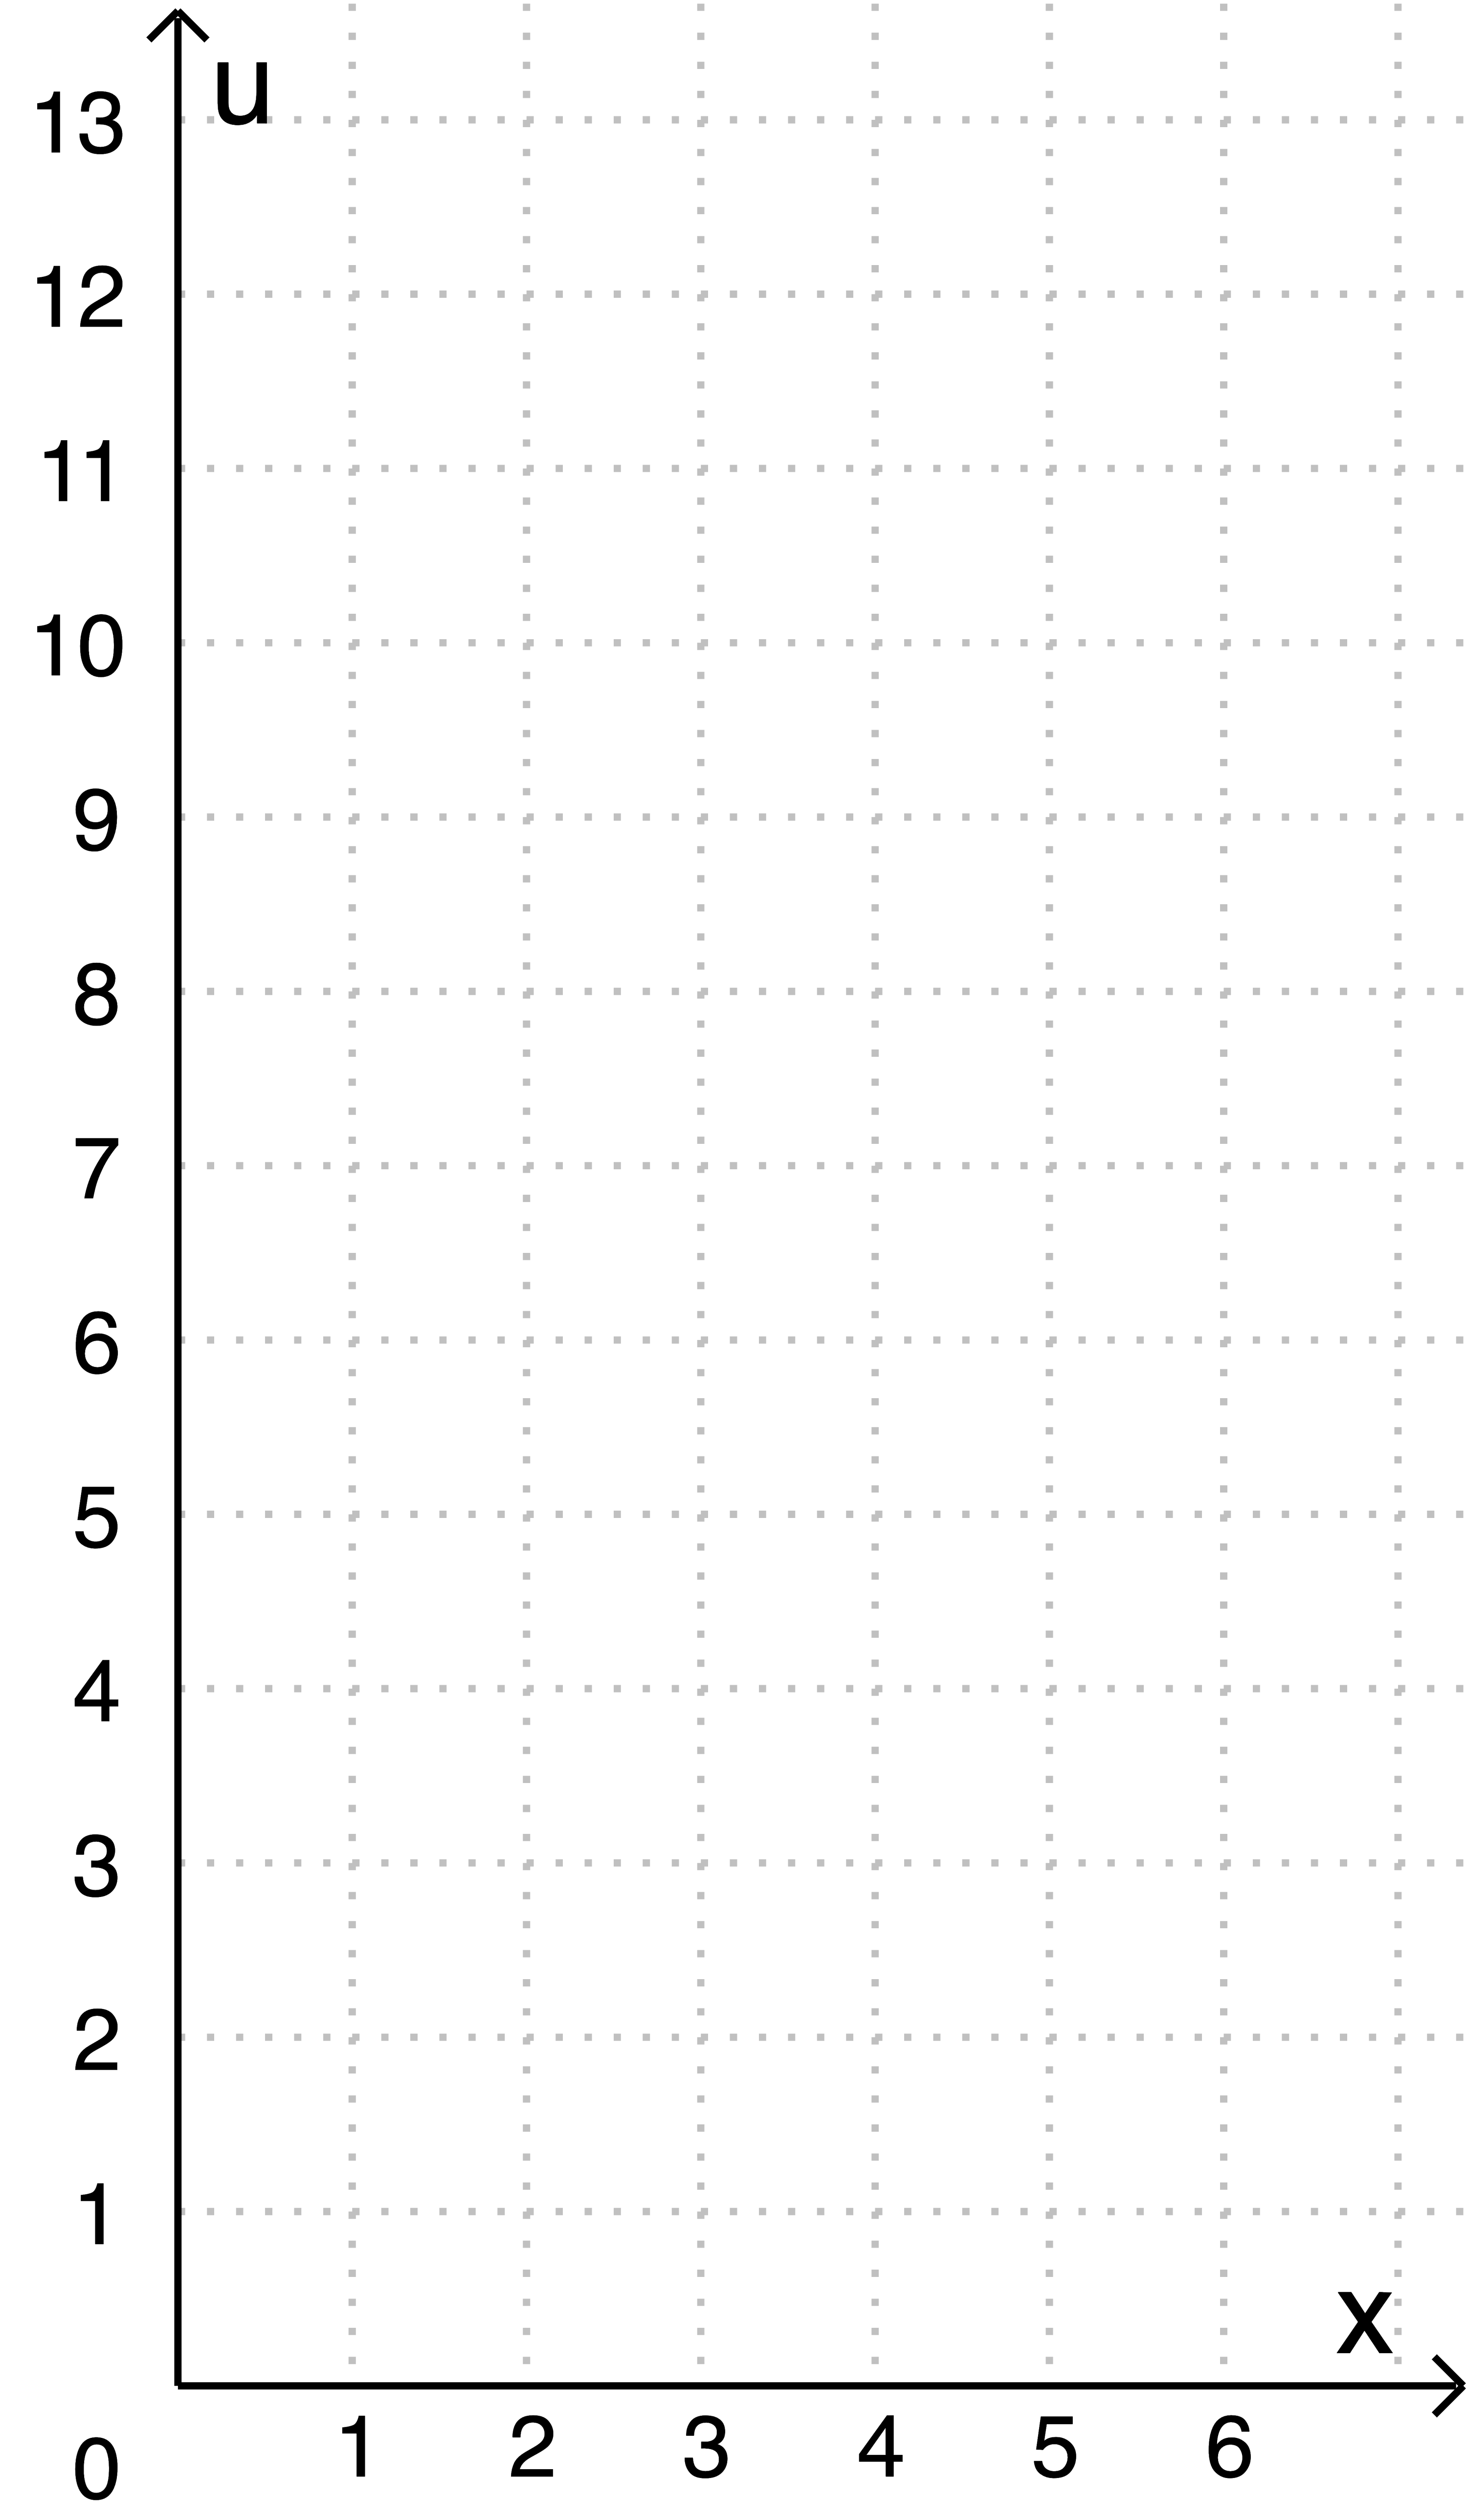
\includegraphics[width=\textwidth]{media/KettenregelLA-1.png}
			            \end{minipage}
			            \begin{minipage}[t]{0.5\textwidth}
				            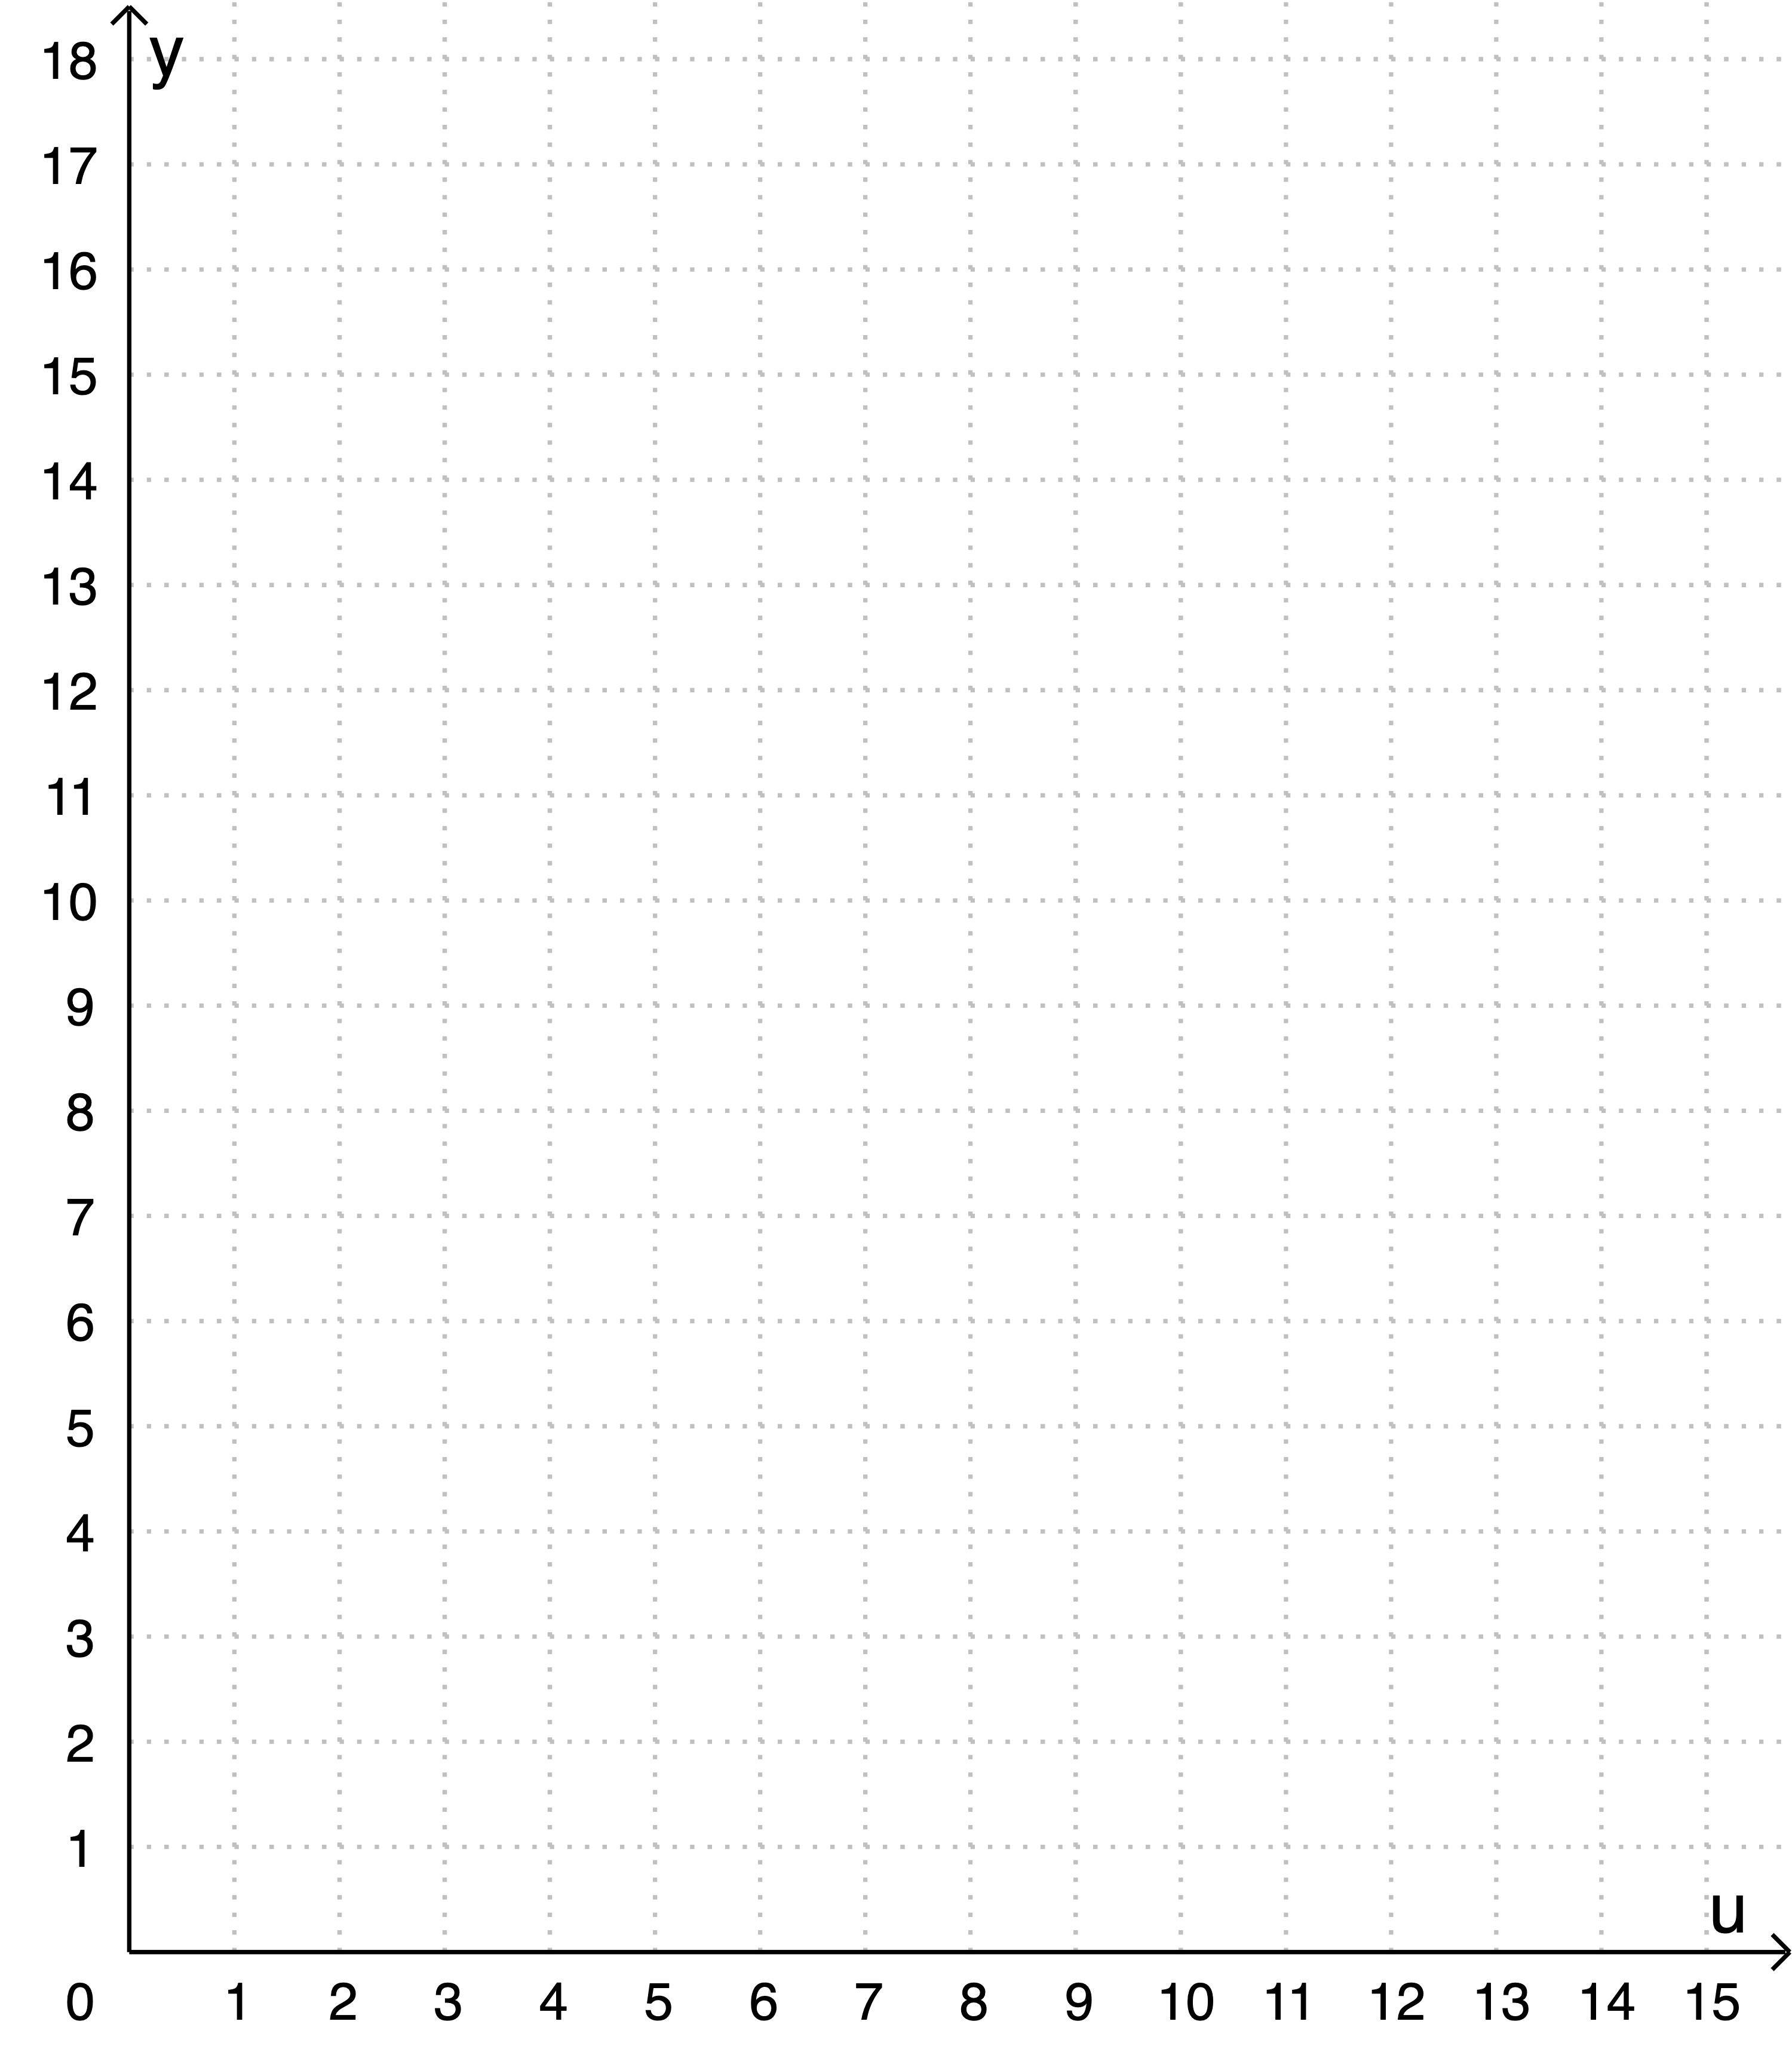
\includegraphics[width=\textwidth]{media/KettenregelLA-2.png}
			            \end{minipage}

			            \begin{center}
				            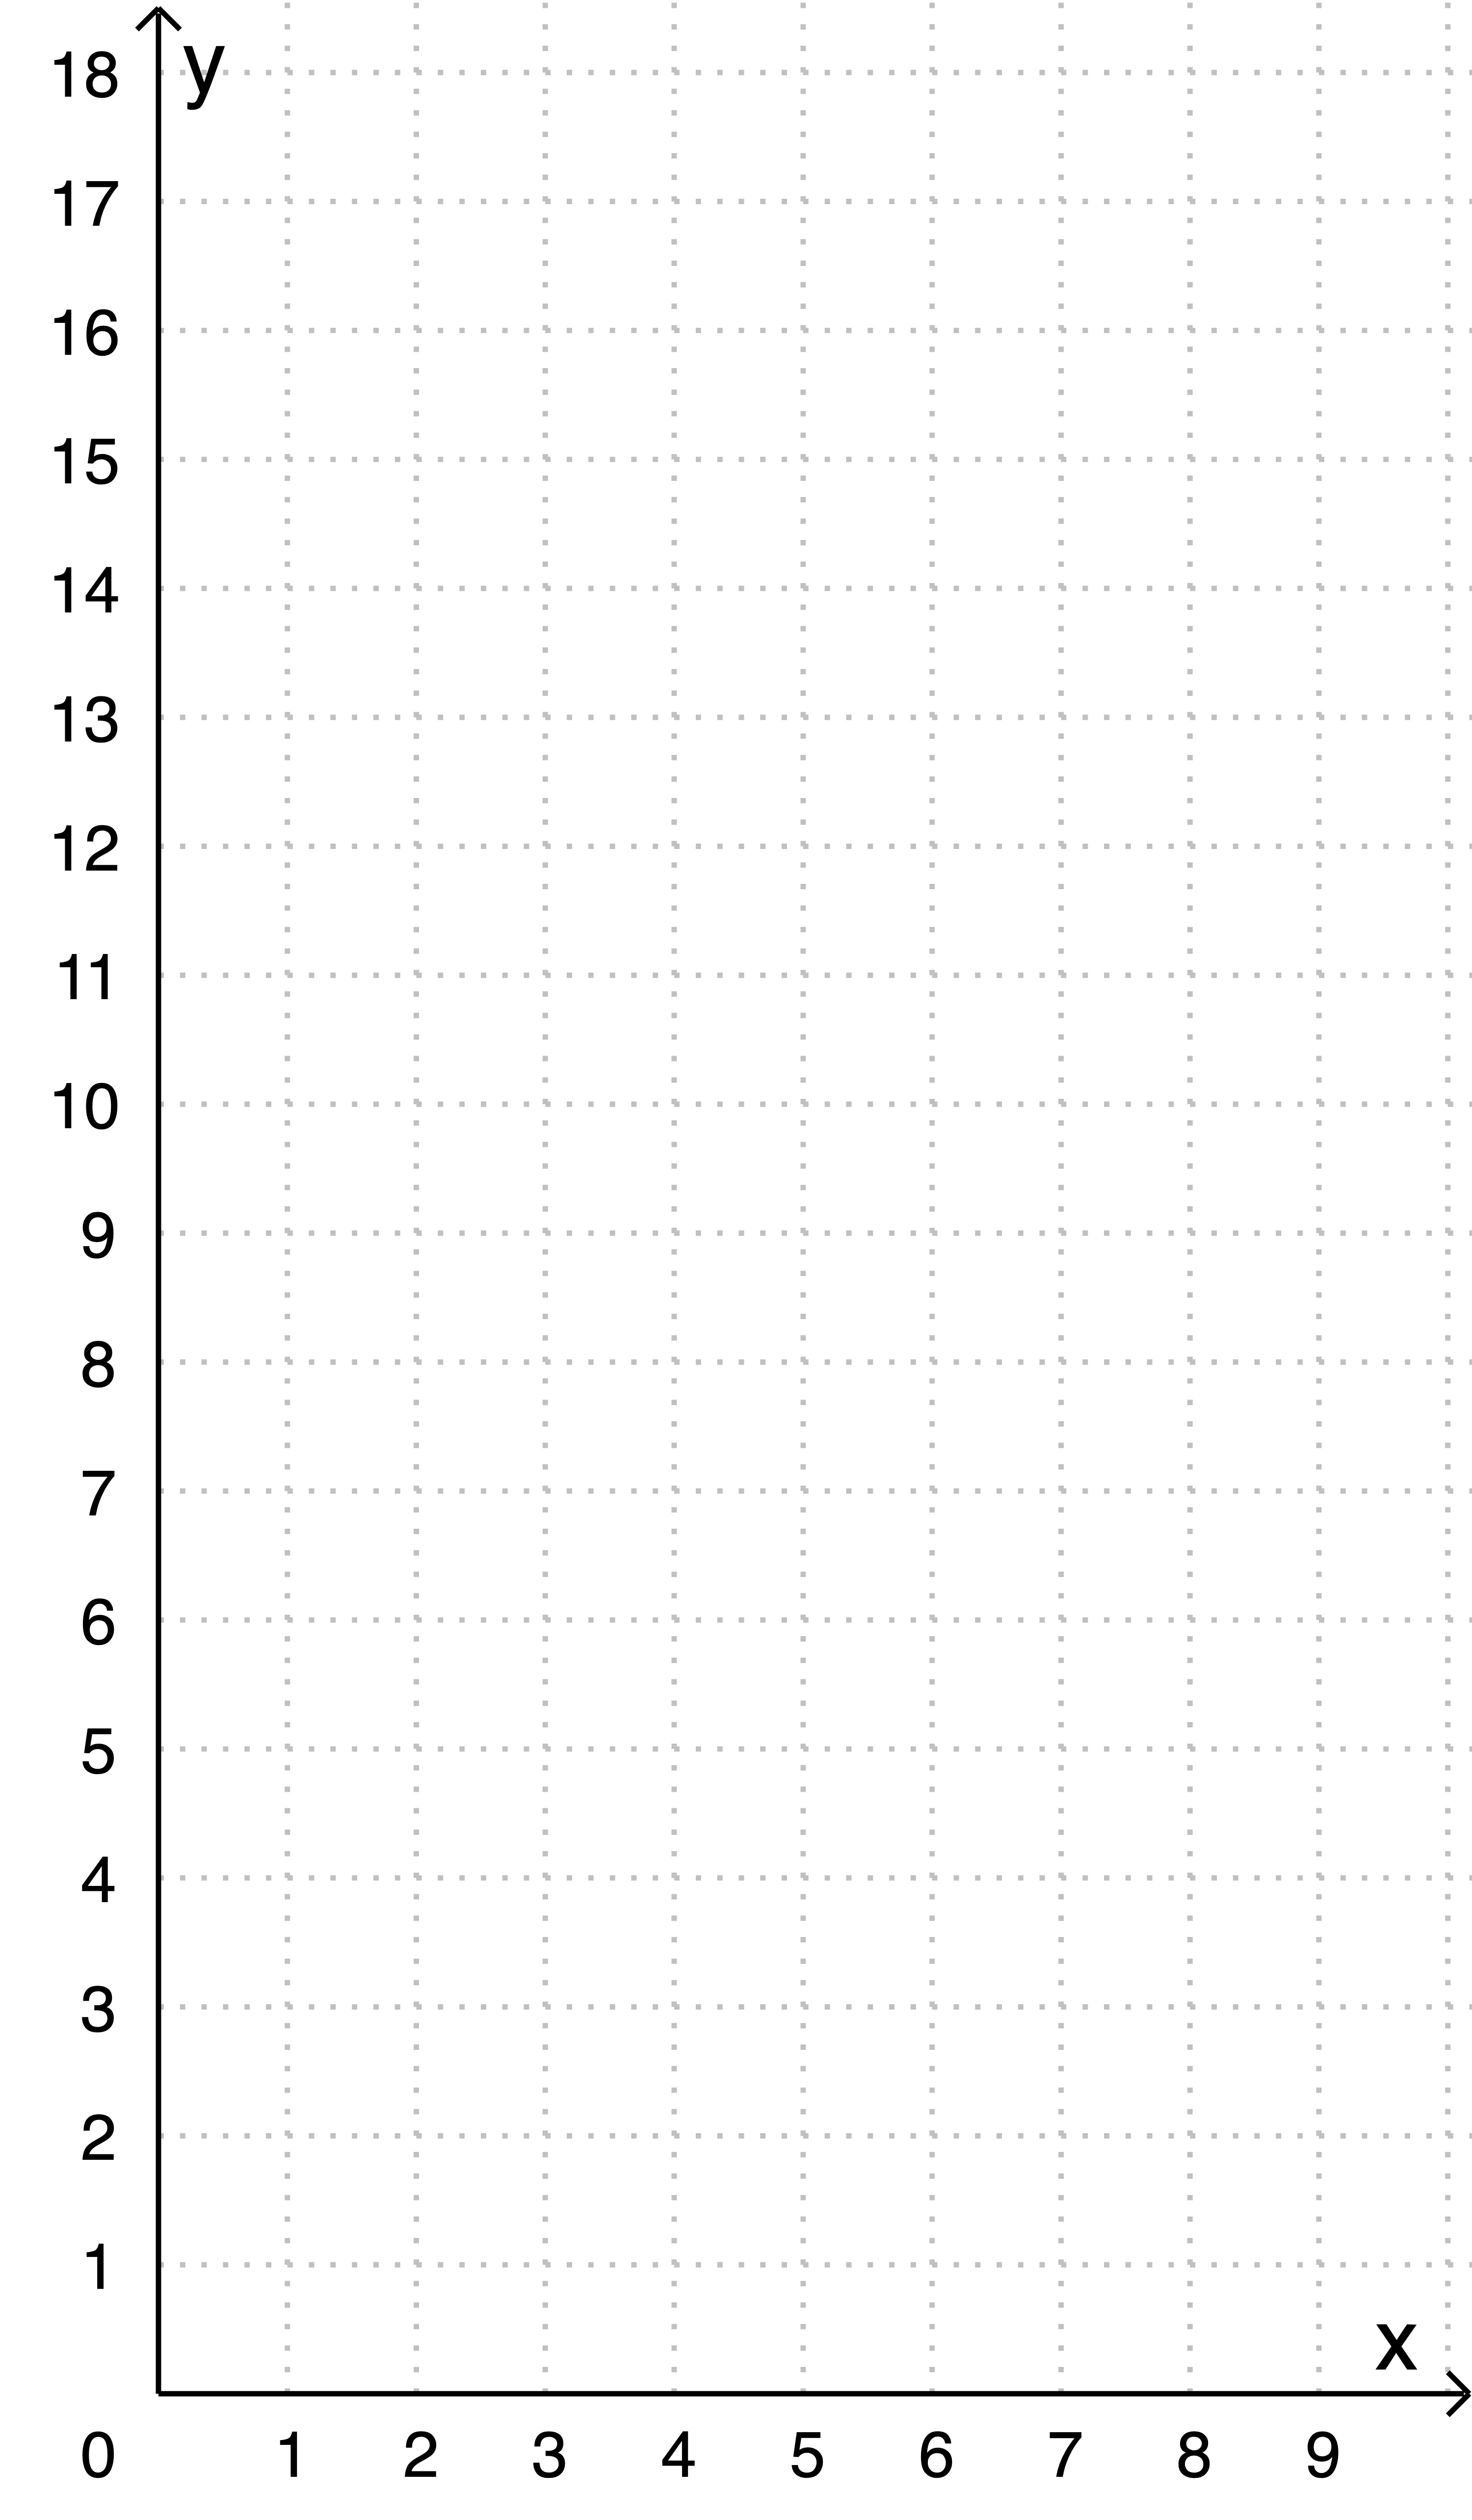
\includegraphics[width=0.36\textwidth]{media/KettenregelLA-3.png}
			            \end{center}




			      \item Welchen Zusammenhang besteht zwischen den Steigungen 	der drei Geraden?

		      \end{enumerate}
		\item Beantworten Sie dieselben Fragen, aber allgemein mit den Funktionen $u=ax+b$ und $y=cu+d$.
	\end{enumerate}

\end{LA}

\clearpage

Die Funktion $k(x)=\sqrt{x^2+x}$ ist eine Verkettung oder Komposition der Funktionen $g(x)=x^2+x$ und $f(u)=\sqrt{u}$. Man schreibt dafür $k(x)=f(g(x))$ oder $k(x)=(f\circ g)(x)$. Dabei nennt man $f$ die \emph{äussere} und $g$ die \emph{innere Funktion}.

Die Kettenregel erklärt, wie man die Ableitung von Verkettungen bestimmen kann.

\begin{satz}
	{Die Kettenregel}{}
	Sei $k(x)=f(g(x))$ die Verkettung zweier Funktionen mit $\mathbb{W}_g\subset \mathbb{D}_f$. Ist $g$ an der Stelle $x\in \mathbb{D}_g$ und $f$ an der Stelle $g(x)$ differenzierbar, so ist auch $k$ an der Stelle $x$ differenzierbar und es gilt
	$$k'(x)=f'(g(x))\cdot g'(x)$$

\end{satz}
Dabei ist $f'(g(x))$ die Ableitung der äusseren Funktion an der Stelle $g(x)$ und $g'(x)$ die Ableitung der inneren Funktion. Oft sagt man kurz: \glqq äussere Ableitung mal innere Ableitung\grqq{}.

\begin{bsp}
	{}{}
	Die Funktion $k(x)=\sqrt{x^2+x}$ soll abgeleitet werden. Dazu lesen wir sie als Verkettung der  beiden Funktion $g(x)=x^2+x$ und $f(u)=\sqrt{u}$. Die Ableitung inneren Funktion ist $g'(x) = 2x+1$. Jene der äusseren Funktion $f$ lautet $f'(u)=\frac{1}{2\sqrt{u}}$. So erhalten wir:

	$$k'(x) = \underbrace{\frac{1}{2\sqrt{x^2+x}}}_{\text{aussere Ableitung }f'(g(x))} \cdot \underbrace{(2x+1)}_{\text{innere Ableitung }g'(x)} = \frac{2x+1}{2\sqrt{x^2+x}}$$


\end{bsp}

Mit der Notation $\frac{d}{dx}$ für die Ableitung lässt sich die Kettenregel einfach merken. Betrachten wir dazu wieder das Beispiel $k(x)=\sqrt{x^2+x}$.
Wir lesen die Funktion als Verkettung der Form
$$x\mapsto u = x^2+x \mapsto y= \sqrt{u}$$

Der erste Pfeil steht für die innere Funktion $u(x)=x^2+x$ mit der Ableitung $\frac{du}{dx}=2x+1$. Der zweite Pfeil steht für die äussere Funktion $y(u)=\sqrt{u}$ mit der Ableitung $\frac{dy}{du}=\frac{1}{2\sqrt{u}}$. Die Kettenregel lautet nun:
$$\frac{dy}{dx}= \frac{dy}{du}\cdot \frac{du}{dx} = \frac{1}{2\sqrt{u}} \cdot (2x+1) \stackrel{u=x^2+x}{=} \frac{1}{2\sqrt{x^2+x}}\cdot (2x+1)$$
In dieser Notation entspricht die Kettenregel dem \glqq Kürzen\grqq{} von $du$ im Term $\frac{dy}{du}\cdot \frac{du}{dx}$.\footnote{Korrekterweise ist das aber kein Kürzen, weil die Terme $\frac{dy}{du}$ und $\frac{du}{dx}$ keine Brüche sind, sondern eine Schreibweise für die Ableitung.}

Wir merken uns:
\begin{satz}
	{Kettenregel in der Notation $\frac{d}{dx}$}{}
	$$\frac{dy}{dx}= \frac{dy}{du}\cdot \frac{du}{dx}$$
\end{satz}

\begin{bsp}
	{$f(x)= (x^3+1)^{10}$, $g(x)=\frac{1}{x^2-3}$, $h(x)=\left(\sqrt{x}+x\right)^3 $ }{}
	% \begin{enumerate}
	%     \item $f(x)= (x^3+1)^{10}$ \newline Lese die Funktion als Verkettung $x\mapsto u = x^3+1 \mapsto y=u^{10}$. Dann gilt:
	%     $$\frac{dy}{dx}= \frac{dy}{du}\cdot \frac{du}{dx} =  10u^9 \cdot 3x^2= 10 (x^3+1)^9\cdot   3x^2 = 30x^2(x^3+1)^9$$
	%     \item $g(x)=\frac{1}{x^2-3}$ \newline
	%     Lese die Funktion als Verkettung $x\mapsto u = x^2-3 \mapsto y=u^{-1}$. Dann gilt
	%     $$\frac{dy}{dx}= \frac{dy}{du}\cdot \frac{du}{dx} = -u^{-2} \cdot 2x  = -\frac{1}{(x^2-3)^2} \cdot 2x
	%     = -\frac{2x}{(x^2-3)^2}$$
	%     Diese Funktion könnte man natürlich auch mit der Quotientenregel ableiten.
	%     \item Mit etwas Übung kann man die Zwischenschritte bald auslassen und rechnet direkt
	%     $$h(x)=\left(\sqrt{x}+x\right)^3 \Rightarrow h'(x)=3\left(\sqrt{x}+x\right)^2 \cdot \left(\frac{1}{2\sqrt{x}}+1\right) $$
	% \end{enumerate}

	\vspace{10cm}
\end{bsp}

\begin{proof}
	Sei $k(x) = f(g(x))$. Mit dem Differentialquotienten gilt
	$$k'(x) = \lim_{h\rightarrow0}\frac{k(x+h)-k(x)}{h} = \lim_{h\rightarrow0}\frac{f(g(x+h))-f(g(x))}{h}$$
	Nun betrachten wir $\bar h = g(x+h)-g(x)$. Für $h\rightarrow0$ gilt auch $\bar h \rightarrow 0$.  Weiter ist $g(x+h) = g(x) + \bar h$. Also:

	\begin{align*}
		k'(x) & = \lim_{h\rightarrow0} \frac{f(g(x)+\bar h) -f(g(x))}{h}                                                        \\
		      & = \lim_{h\rightarrow0} \frac{f(g(x)+\bar h) -f(g(x))}{h} \cdot \frac{\bar h}{ \bar h}                           \\
		      & = \lim_{h\rightarrow0} \frac{f(g(x)+\bar h) -f(g(x))}{\bar h} \cdot \frac{\bar h}{h}                            \\
		      & = \lim_{h\rightarrow0} \frac{f(g(x)+\bar h) -f(g(x))}{\bar h} \cdot \frac{g(x+h)-g(x)}{ h}                      \\
		      & = \lim_{h\rightarrow0} \frac{f(g(x)+\bar h) -f(g(x))}{\bar h} \cdot \lim_{h\rightarrow0} \frac{g(x+h)-g(x)}{ h} \\
		      & = f'(g(x)) \cdot g'(x)
	\end{align*}
\end{proof}

\clearpage
\begin{ueb}
	{}{}
	\begin{enumerate}
		\item Bestimme die Ableitung der folgenden Funktionen:
		      \begin{enumerate}
			      \item $y = (x^2+1)^8$
			      \item $y = \sqrt{3x^2+1}$
			      \item $y= \frac{1}{(x^2+1)^3}= (x^2+1)^{-3}$
		      \end{enumerate}
		\item Die Kettenregel kann auch auf die Verkettung von mehr als zwei Funktionen angewendet werden. Leite die folgenden Funktion ab:
		      $$y = \sqrt{(x^2+1)^3+x}$$
		\item Bestimme den Wert des Parameters \( a \in \mathbb{R} \) so, dass für die Funktion \( f \) gilt: \( f'(1) = 24 \).
		      \begin{enumerate}
			      \item \( f(x) = (2x - a)^3 \)
			      \item \( f(x) = -\dfrac{6}{\sqrt{a x}} \) (Hinweis: Du kannst die Funktion auf verschiedene Arten Ableiten: Direkt mit der Quotientenregel oder zuerst umformen zu $f(x) = -6 (ax)^{-1/2}$ )
			      \item \( f(x) = \dfrac{2a}{a - 4x} \)
		      \end{enumerate}


		\item Bestimme die Gleichung der Tangente im Punkte \( P \) des Graphen der gegebenen Funktion \( f\colon x \mapsto y \).
		      \begin{enumerate}
			      \item \( y = \dfrac{3 - x}{3x + 1}, \quad P(-2 , y_P) \)
			      \item \( y = \dfrac{x^2 + 5}{x^2 - 2}, \quad P(3 , y_P) \)
			      \item \( y = \sqrt{3x + 1}, \quad P(1 ,  y_P) \)
		      \end{enumerate}

		\item An den Graphen der Funktion \( f\colon x \mapsto y \) werden Tangenten mit der Steigung \( m \) gelegt. Welche Koordinaten haben die Berührungspunkte?
		      \begin{enumerate}
			      \item \( y = \dfrac{x + 2}{2x}, \quad m = -1 \)
			      \item \( y = \dfrac{x^2 - 5}{x + 1}, \quad m = \frac{5}{4} \)
			            %\item \( y = \dfrac{x^3}{x - 2}, \quad m = -4 \) 3 Lösungen!
		      \end{enumerate}

		\item Zeige: Die Gerade \( g\colon y = 2x \) ist Tangente der Kurve \( f\colon y = 4 \sqrt{2x - 4} \).


	\end{enumerate}
\end{ueb}

\clearpage
\emph{Lösungen:}
\begin{enumerate}
	\item Bestimme die Ableitung der folgenden Funktionen:
	      \begin{enumerate}
		      \item \( y' = 8(x^2+1)^7 \cdot 2x = 16x(x^2+1)^7 \)
		      \item \( y' = \dfrac{1}{2\sqrt{3x^2+1}} \cdot 6x = \dfrac{3x}{\sqrt{3x^2+1}} \)
		      \item \( y' = -3(x^2+1)^{-4} \cdot 2x = \dfrac{-6x}{(x^2+1)^4} \)
	      \end{enumerate}

	\item Lese die Funktion als Verkettung
	      $$ x \mapsto u = (x^2+1)^3+x \mapsto y = \sqrt{u}$$

	      \[
		      y' = \dfrac{1}{2\sqrt{(x^2+1)^3+x}} \cdot \left(3(x^2+1)^2 \cdot 2x + 1\right)
	      \]

	\item Bestimme den Wert des Parameters \( a \in \mathbb{R} \), so dass \( f'(1) = 24 \).
	      \begin{enumerate}
		      \item \( f'(x) = 3(2x - a)^2 \cdot 2 \Rightarrow f'(1) = 6(2 - a)^2 = 24 \Rightarrow a = 0 \text{ oder } a = 4 \)
		      \item \( f'(x) = \dfrac{3}{x\sqrt{ax}} \Rightarrow f'(1) = \dfrac{3}{\sqrt{a}} = 24 \Rightarrow a = \dfrac{1}{64} \)
		      \item \( f'(x) = \dfrac{8a}{(a - 4x)^2} \Rightarrow f'(1) = \dfrac{8a}{(a - 4)^2} = 24 \Rightarrow a = 3 \text{ oder } a = \frac{16}{3} \)
	      \end{enumerate}

	\item Bestimme die Gleichung der Tangente im Punkt \( P \).
	      \begin{enumerate}
		      \item \( y = -\dfrac{2}{5}x - \dfrac{9}{5} \)
		      \item \( y = -\dfrac{6}{7}x + \dfrac{32}{7} \)
		      \item \( y = \dfrac{3}{4}x + \dfrac{5}{4} \)
	      \end{enumerate}

	\item Koordinaten der Berührungspunkte bei gegebener Steigung:
	      \begin{enumerate}
		      \item \( B_1 = (1, 1.5); B_2 = (-1, -0.5) \)
		      \item \( B_1 = (3, 1); B_2 = (-5, -5) \)
	      \end{enumerate}

	\item Zeige: \( g(x) = 2x \) ist Tangente an \( f(x) = 4\sqrt{2x - 4} \)

	      $$f'(x) = g'(x) \iff \dfrac{4}{\sqrt{2x - 4}} = 2 \iff x = 4$$

	      Prüfe ob $f(4) = g(4)$ ist:
	      $$ f(4) = 4\sqrt{2\cdot 4 -4} = 8, \quad g(4) = 2\cdot 4 = 8$$

	      Also ist die Gerade \( g \) Tangente an den Graphen von \( f \) im Punkt \( (4, 8) \).
\end{enumerate}
















































\clearpage
\subsection{Die Ableitung der elementaren Funktionen}
\subsubsection{ Die Ableitung trigonometrischer Funktionen}
\begin{LA}
	{Die Ableitung der Sinusfunktion}{}
	\begin{enumerate}
		\item Unten ist der Graph der Sinusfunktion im Bereich $x \in [0, 2\pi]$ dargestellt. Skizzieren Sie in das gleiche Koordinatensystem den ungefähren Verlauf des Graphen der Ableitung $\frac{d}{dx} \sin(x)$, indem Sie
		      die Steigung der Sinusfunktion schätzen. Was vermuten Sie?
		      \begin{center}
			      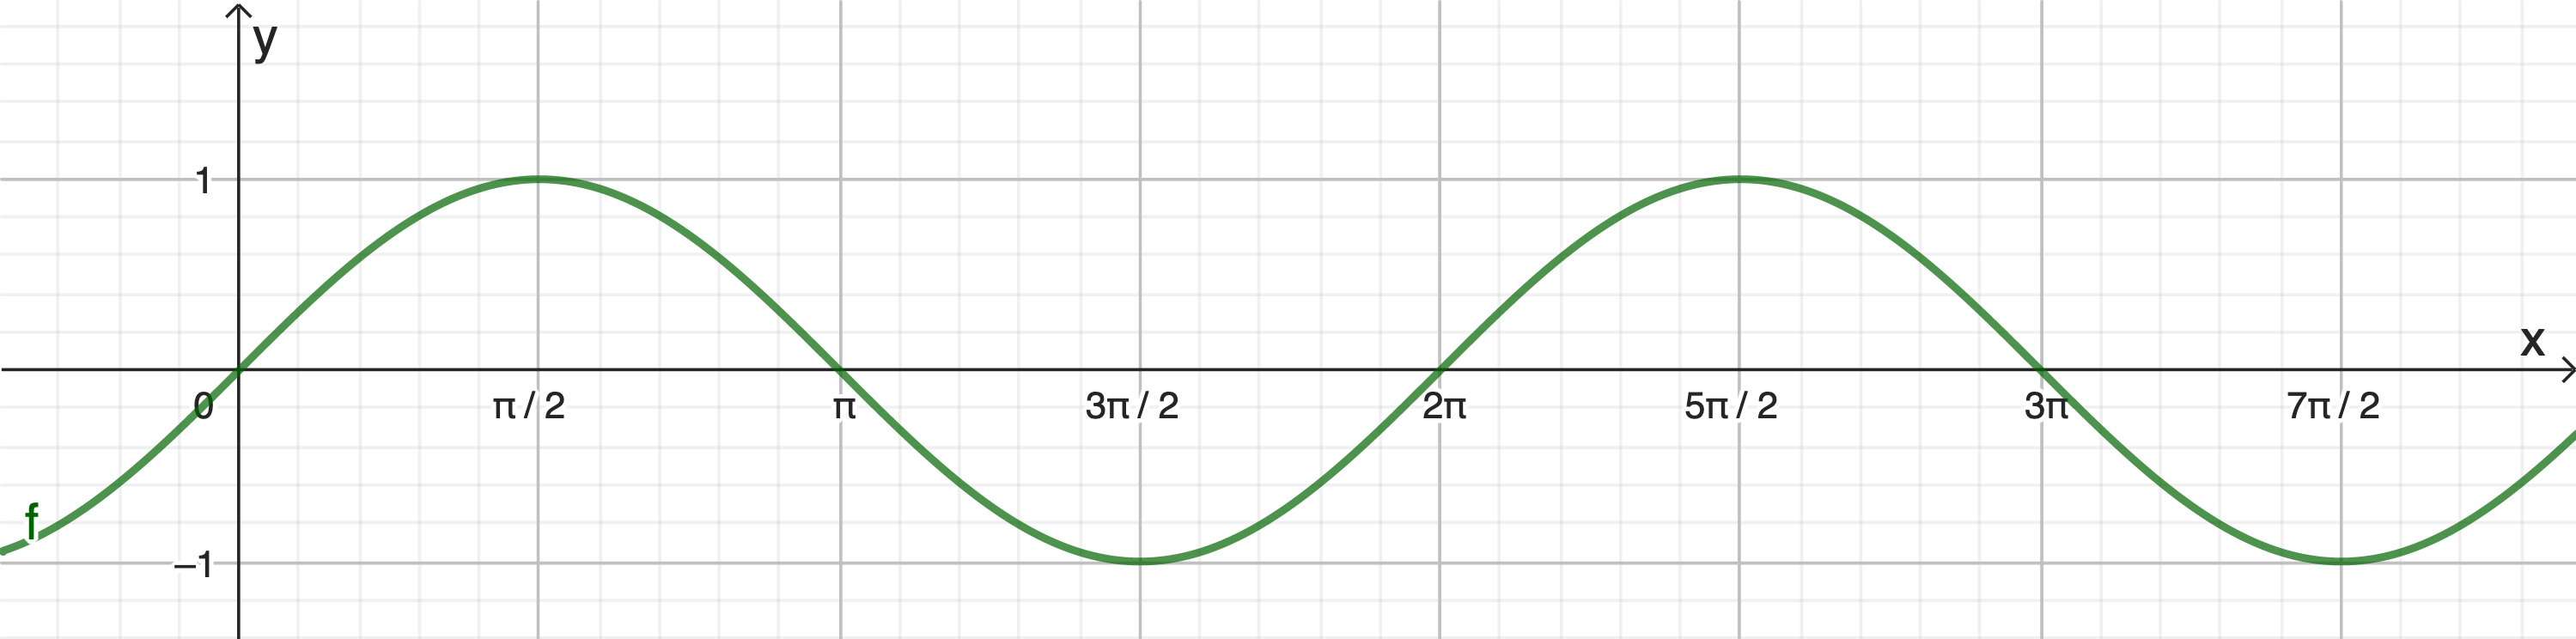
\includegraphics[]{media/sinuskurve.png}
		      \end{center}
	\end{enumerate}
	In den folgenden Aufgaben wollen wir die Vermutung durch Betrachtungen am Differentialquotienten stützen. Die Ableitung der Sinusfunktion ist nach Definition der Grenzwert
	$$
		\lim_{h\rightarrow0} \frac{\sin(x+h)-\sin(x)}{h}
	$$
	Diesen Bruch kann man mit den sogenannten Additionstheoremen vereinfachen: Für alle Winkel $\alpha$ und $\beta$ gilt:
	\begin{align*}
		\sin(\alpha + \beta)  & = \sin(\alpha) \cos(\beta) +\cos(\alpha) \sin(\beta) \\
		\cos( \alpha + \beta) & = \cos(\alpha)\cos (\beta) - \sin(\alpha)\sin(\beta)
	\end{align*}
	\begin{enumerate}[resume]
		\item Zeigen Sie unter Verwendung der Additionstheoreme, dass man den Differenzenquotienten so umformen kann:
		      $$
			      \frac{\sin(x+h)-\sin(x)}{h} = \sin(x)\cdot \frac{\cos(h)-1}{h} +\cos(x) \cdot \frac{\sin(h)}{h}
		      $$
		\item Was passiert mit diesem Term, wenn $h$ gegen Null strebt? Stellen Sie Ihr Taschenrechner auf \emph{Bogenmass (rad)} ein und füllen Sie die folgende Tabelle aus.
		      \begin{center}


			      \begin{tabular}{c|c|c}

				      $h$ (rad) & $\quad \frac{\cos(h)-1}{h} \quad$ & $\quad \frac{\sin(h)}{h} \quad$ \\ \hline
				      $0.1$     &                                   & \parbox[0pt][3em][c]{0cm}{}     \\ \hline
				      $0.01$    &                                   & \parbox[0pt][3em][c]{0cm}{}     \\\hline
				      $0.001$   &                                   & \parbox[0pt][3em][c]{0cm}{}
			      \end{tabular}
		      \end{center}
		      Was vermuten Sie für die Grenzwerte für $h \rightarrow 0$? Was ist demnach die Ableitung der Sinusfunktion?

		\item Gehen Sie gleich vor, um die Ableitung der Cosinusfunktion zu bestimmen.
		\item In der Tabelle in Aufgabe 3 haben Sie den Taschenrechner auf Bogenmass eingestellt. Was ändert sich, wenn Sie im Gradmass arbeiten? Welche Auswirkung hat das auf die Ableitung der Sinusfunktion?
	\end{enumerate}

\end{LA}
\clearpage

Mit dem Differentialquotienten können wir die Ableitung der Sinusfunktion bestimmen. Dazu verwenden wir das Additionstheorem (AT) für den Sinus:
$$  \sin(\alpha + \beta) = \sin(\alpha) \cos(\beta) +\cos(\alpha) \sin(\beta) $$

Für den Differenzialquotienten folgt dann
\begin{align*}
	\frac{d}{dx} \sin(x) & = \lim_{h\rightarrow0} \frac{\sin(x+h)-\sin(x)}{h}                                                                                     \\
	                     & \stackrel{AT}{=} \lim_{h\rightarrow0} \frac{\sin(x)\cos(h)+\cos(x)\sin(h)-\sin(x)}{h}                                                  \\
	                     & = \lim_{h\rightarrow0} \frac{\sin(x) \left(\cos(h)-1\right)+\cos(x)\sin(h)}{h}                                                         \\
	                     & = \sin(x)\cdot \left[\lim_{h\rightarrow0}\frac{\cos(h)-1}{h}\right] +\cos(x) \cdot \left[\lim_{h\rightarrow0}\frac{\sin(h)}{h} \right]
\end{align*}

Die beiden Grenzwerte in den eckigen Klammern sind nicht einfach zu bestimmen. Die folgenden Hilfssätze – in der Mathematik spricht man von Lemmata – helfen uns weiter.

\begin{satz}
	{Lemma 1}{}
	Sei $h$ ein Winkel im Bogenmass, dann gilt
	$$\lim_{h\rightarrow0}\frac{\sin(h)}{h} =1$$
\end{satz}
\begin{proof}
	Betrachten wir die folgenden drei Flächen im Einheitskreis:
	\begin{center}
		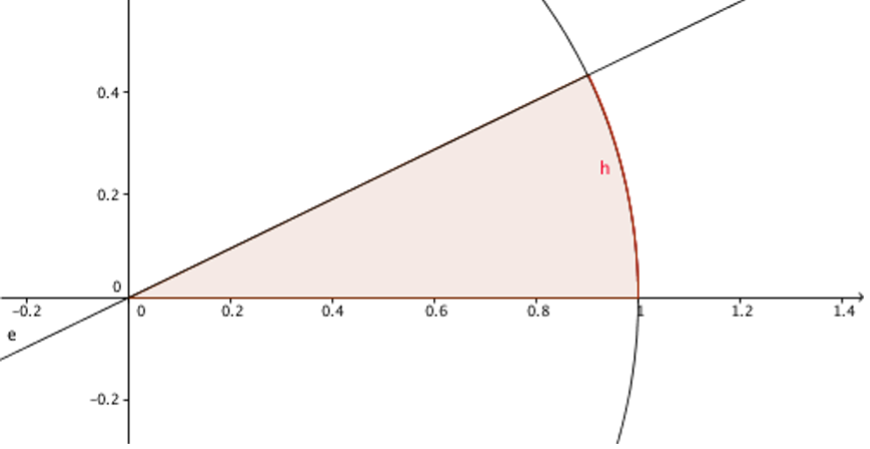
\includegraphics{media/bewSin1.png}
	\end{center}
	Der Flächeninhalt des Kreissektors mit Bogen der Länge $h$ beträgt
	$$ A_{\text{Sektor}} = \pi r^2\cdot \frac{h}{2\pi} = \frac{1}{2} h
	$$
	\begin{center}
		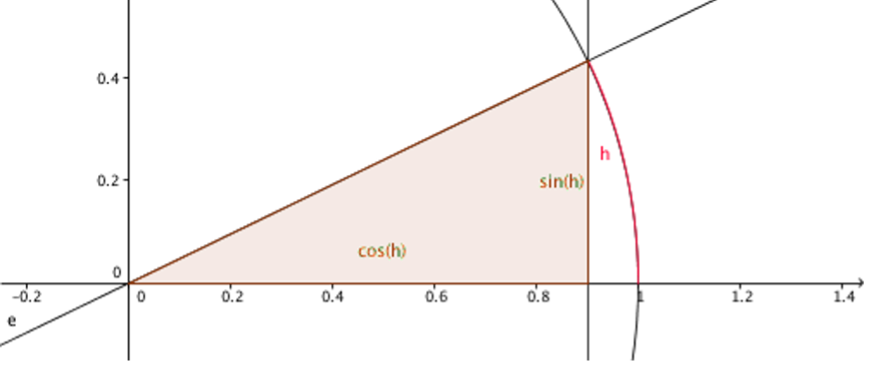
\includegraphics{media/bewSin2.png}
	\end{center}
	Die Fläche des im Kreissektor einbeschriebenen, rechtwinkligen Dreiecks hat den Inhalt
	$$A_{\text{Einb}} = \frac{1}{2}\sin(h)\cos(h) $$

	\begin{center}
		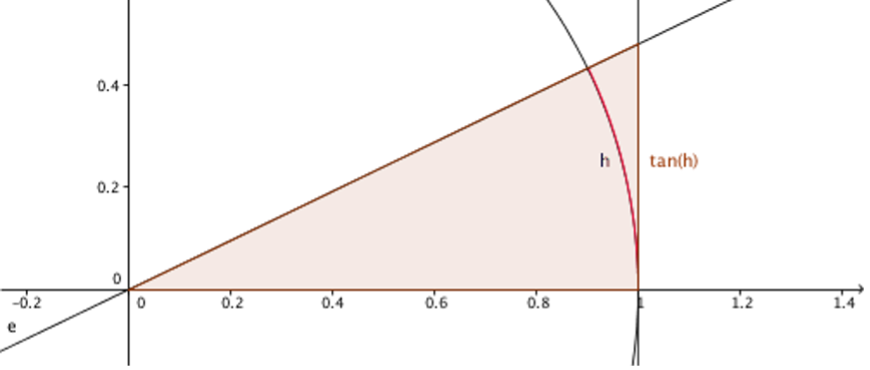
\includegraphics{media/bewSin3.png}
	\end{center}
	Die Fläche des dem Kreissektor umbeschriebenen, rechtwinkligen Dreiecks beträgt
	$$A_{\text{Umb}} =\frac{1}{2}\cdot1\cdot \tan(h) = \frac{\sin(h)}{2\cos(h)} $$
	% \begin{tabular}{c|p{8cm}}
	%     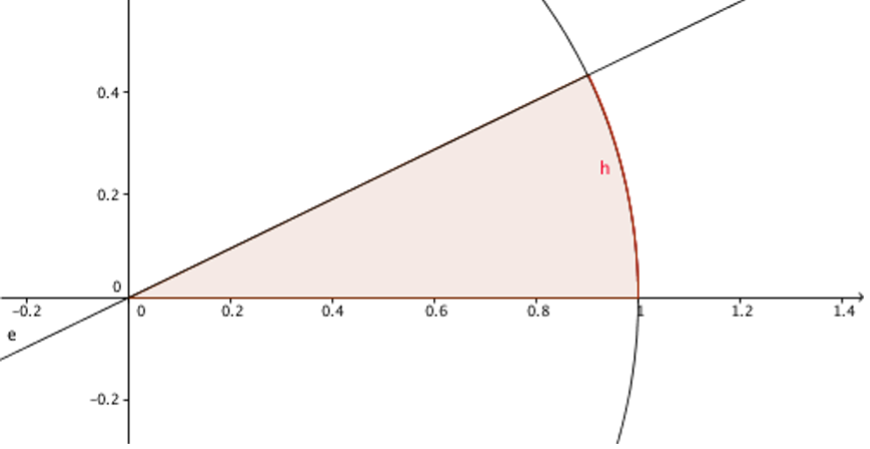
\includegraphics{media/bewSin1.png} & Der Flächeninhalt des Kreissektors mit Bogen der Länge $h$ beträgt
	%     $$ A_{\text{Sektor}} = \pi r^2\cdot \frac{h}{2\pi} = \frac{1}{2} h
	%     $$ \\ \hline 
	%     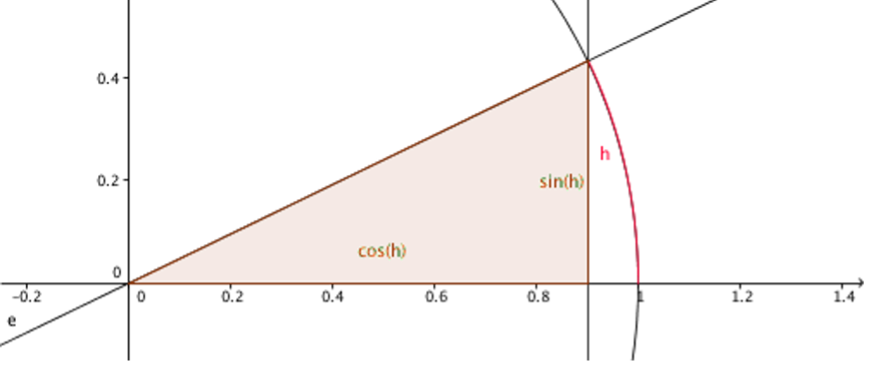
\includegraphics{media/bewSin2.png} & Die Fläche des im Kreissektor einbeschriebenen, rechtwinkligen Dreiecks beträgt
	%     $$A_{\text{Einb}} = \frac{1}{2}\sin(h)\cos(h) $$
	%      \\ \hline
	%     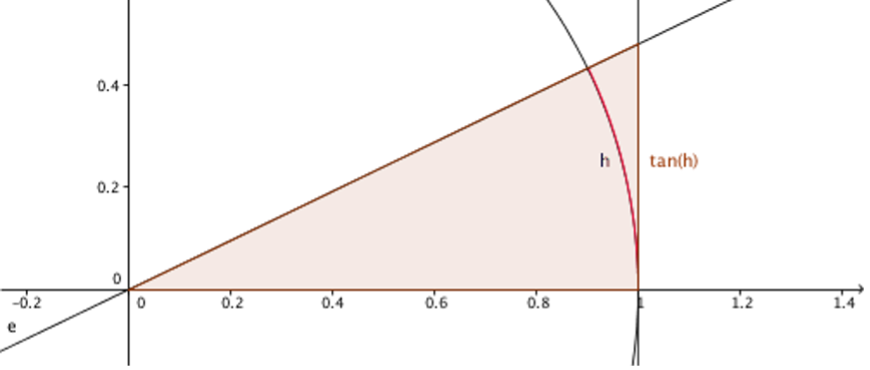
\includegraphics{media/bewSin3.png} & Die Fläche des dem Kreissektor umbeschriebenen, rechtwinkligen Dreiecks beträgt
	%     $$A_{\text{Umb}} =\frac{1}{2}\cdot1\cdot \tan(h) = \frac{\sin(h)}{2\cos(h)} $$



	% \end{tabular}

	Für alle $h \in \left]0, \frac{\pi}{2} \right[$ gilt
	\begin{align*}
		A_{\text{Einb}}           & \le A_{\text{Sektor}} \le  A_{\text{Umb}}      &                           \\
		\frac{1}{2}\sin(h)\cos(h) & \le \frac{1}{2} h \le \frac{\sin(h)}{2\cos(h)} & | \cdot \frac{2}{\sin(h)} \\
		\cos(h)                   & \le \frac{h}{\sin(h)} \le \frac{1}{\cos(h)}    & | \text{Kehrwert}         \\
		\frac{1}{\cos(h)}         & \ge \frac{\sin(h)}{h} \ge \cos(h)              &
	\end{align*}
	Für negative Werte von $h$ führt eine analoge Abschätzung zur selben Ungleichung.

	Für $h\rightarrow0$ gilt dann:
	$$
		\frac{1}{1} \ge \lim_{h\rightarrow0}\frac{\sin(h)}{h} \ge 1
	$$
	Daraus folgt das Lemma.
\end{proof}

\begin{satz}
	{Lemma 2}{}
	Sei $h$ ein Winkel im Bogenmass, dann gilt
	$$\lim_{h\rightarrow0}\frac{\cos(h)-1}{h} =0$$
\end{satz}
\begin{proof}
	Als Hilfsmittel wird der trigonometrischen Pythagoras benötigt: $\sin^2(h)+\cos^2(h) =1$
	\begin{align*}
		\frac{\cos(h)-1}{h} & = \frac{\cos(h)-1}{h}\cdot \frac{\cos(h)+1}{\cos(h)+1} \\
		                    & = \frac{\cos^2(h)-1}{h(\cos(h)+1)}                     \\
		                    & \stackrel{TP}{=} - \frac{\sin^2(h)}{h(\cos(h)+1)}      \\
		                    & = -\frac{\sin(h)}{h}\cdot \frac{\sin(h)}{\cos(h)+1}
	\end{align*}

	Für $h\rightarrow0$ folgt dann
	$$
		\lim_{h\rightarrow0}\frac{\cos(h)-1}{h} =\lim_{h\rightarrow0}\left(-\frac{\sin(h)}{h}\cdot \frac{\sin(h)}{\cos(h)+1}\right) = -1 \cdot \frac{0}{1+1} = 0
	$$
\end{proof}
Dank den beiden Lemmata können wir nun die Ableitung der Sinusfunktion berechnen:
$$
	\frac{d}{dx} \sin(x) = \sin(x)\cdot \left[\lim_{h\rightarrow0}\frac{\cos(h)-1}{h}\right] +\cos(x) \cdot \left[\lim_{h\rightarrow0}\frac{\sin(h)}{h} \right] = \sin(x) \cdot 0 + \cos(x) \cdot 1 = \cos(x)
$$
Analog lässt sich auch die Ableitung der Cosinusfunktion herleiten.
\begin{satz}{Die Ableitung von Sinus und Cosinus}{}
	Die Sinus- und Cosinusfunktion sind an jeder Stelle differenzierbar und für die Ableitungen gilt
	$$
		\frac{d}{dx}\sin(x) = \cos(x)
	$$
	und
	$$
		\frac{d}{dx}\cos(x) = -\sin(x)
	$$
	($x$ in rad)
\end{satz}

Mit der Quotientenregel kann man leicht auch die Ableitung der Tangensfunktion bestimmen (siehe Übungen)
\begin{satz}
	{Sie Ableitung der Tangensfunktion}{}
	Die Tangensfunktion ist an jeder Stelle im Definitionsbereich differenzierbar und es gilt:
	$$
		\frac{d}{dx}\tan(x) = \frac{1}{\cos^2(x)} = 1+ \tan^2(x)
	$$
\end{satz}

\clearpage
\begin{ueb}
	{}{}
	\begin{enumerate}
		\item Bestimme die Ableitung der folgenden Funktionen:
		      \begin{enumerate}
			      \item $y= 3x\cdot \cos(x)$
			      \item $y= \sin(2x)$
			      \item $y= 2x\tan(x)$
			      \item $y= \frac{\sin(x)}{x}$
			      \item $ y= \frac{x}{\cos(x)}$
			      \item $y =\sin^2(x) = (\sin(x))^2$
			      \item $y = \sin(x^2)$
			      \item $y=\sqrt{\cos(x)}$
		      \end{enumerate}
		\item Bestimme die Gleichung der Tangente im Punkt $P$ des Graphen der gegebenen Funktion
		      \begin{enumerate}
			      \item $ y= \cos(x), \quad P=\left(\frac{\pi}{2}, y_P\right)$
			      \item $ y= \tan(x), \quad P=\left(\frac{\pi}{4}, y_P\right)$
		      \end{enumerate}
		\item Verwenden Sie $\tan(x) = \frac{\sin(x)}{\cos(x)}$ und die Quotientenregel, um die Regel für die Ableitung der Tangensfunktion herzuleiten:
		      $$
			      \frac{d}{dx}\tan(x) = \frac{1}{\cos^2(x)} = 1+ \tan^2(x)
		      $$
	\end{enumerate}
\end{ueb}

\clearpage
\emph{Lösungen:}
\begin{enumerate}
	\item Bestimme die Ableitung der folgenden Funktionen:
	      \begin{enumerate}
		      \item $y' = 3\cos(x) - 3x\sin(x)$
		      \item $y' = 2\cos(2x)$
		      \item $y' = 2\tan(x) + \frac{2x}{\cos^2(x)}$
		      \item $y' = \frac{x\cos(x)-\sin(x)}{x^2}$
		      \item $y' = \frac{\cos(x)+x\sin(x)}{\cos^2(x)}$
		      \item $y' = 2\sin(x)\cos(x)$
		      \item $y' = 2x\cos(x^2)$
		      \item $y' = -\frac{\sin(x)}{2\sqrt{\cos(x)}}$
	      \end{enumerate}
	\item Bestimme die Gleichung der Tangente im Punkt $P$ des Graphen der gegebenen Funktion
	      \begin{enumerate}
		      \item $y= -x+\frac{\pi}{2}$
		      \item $y= 2x+1-\frac{\pi}{2}$
	      \end{enumerate}
	\item Der trigonometrische Pythagoras $\cos^2(x)+\sin^2(x) = 1$ kann nützlich sein\dots
\end{enumerate}






































\clearpage
\subsubsection{Die Ableitung der Exponentialfunktionen}
\begin{LA}
	{Die Ableitung der Exponentialfunktionen}{}
	\begin{enumerate}
		\item Betrachten Sie den Graphen der Funktion $f(x)=10^x$. Schätzen Sie den Wert von $f'(-0.4)$, indem Sie die entsprechende Tangente einzeichnen.
		      \begin{center}
			      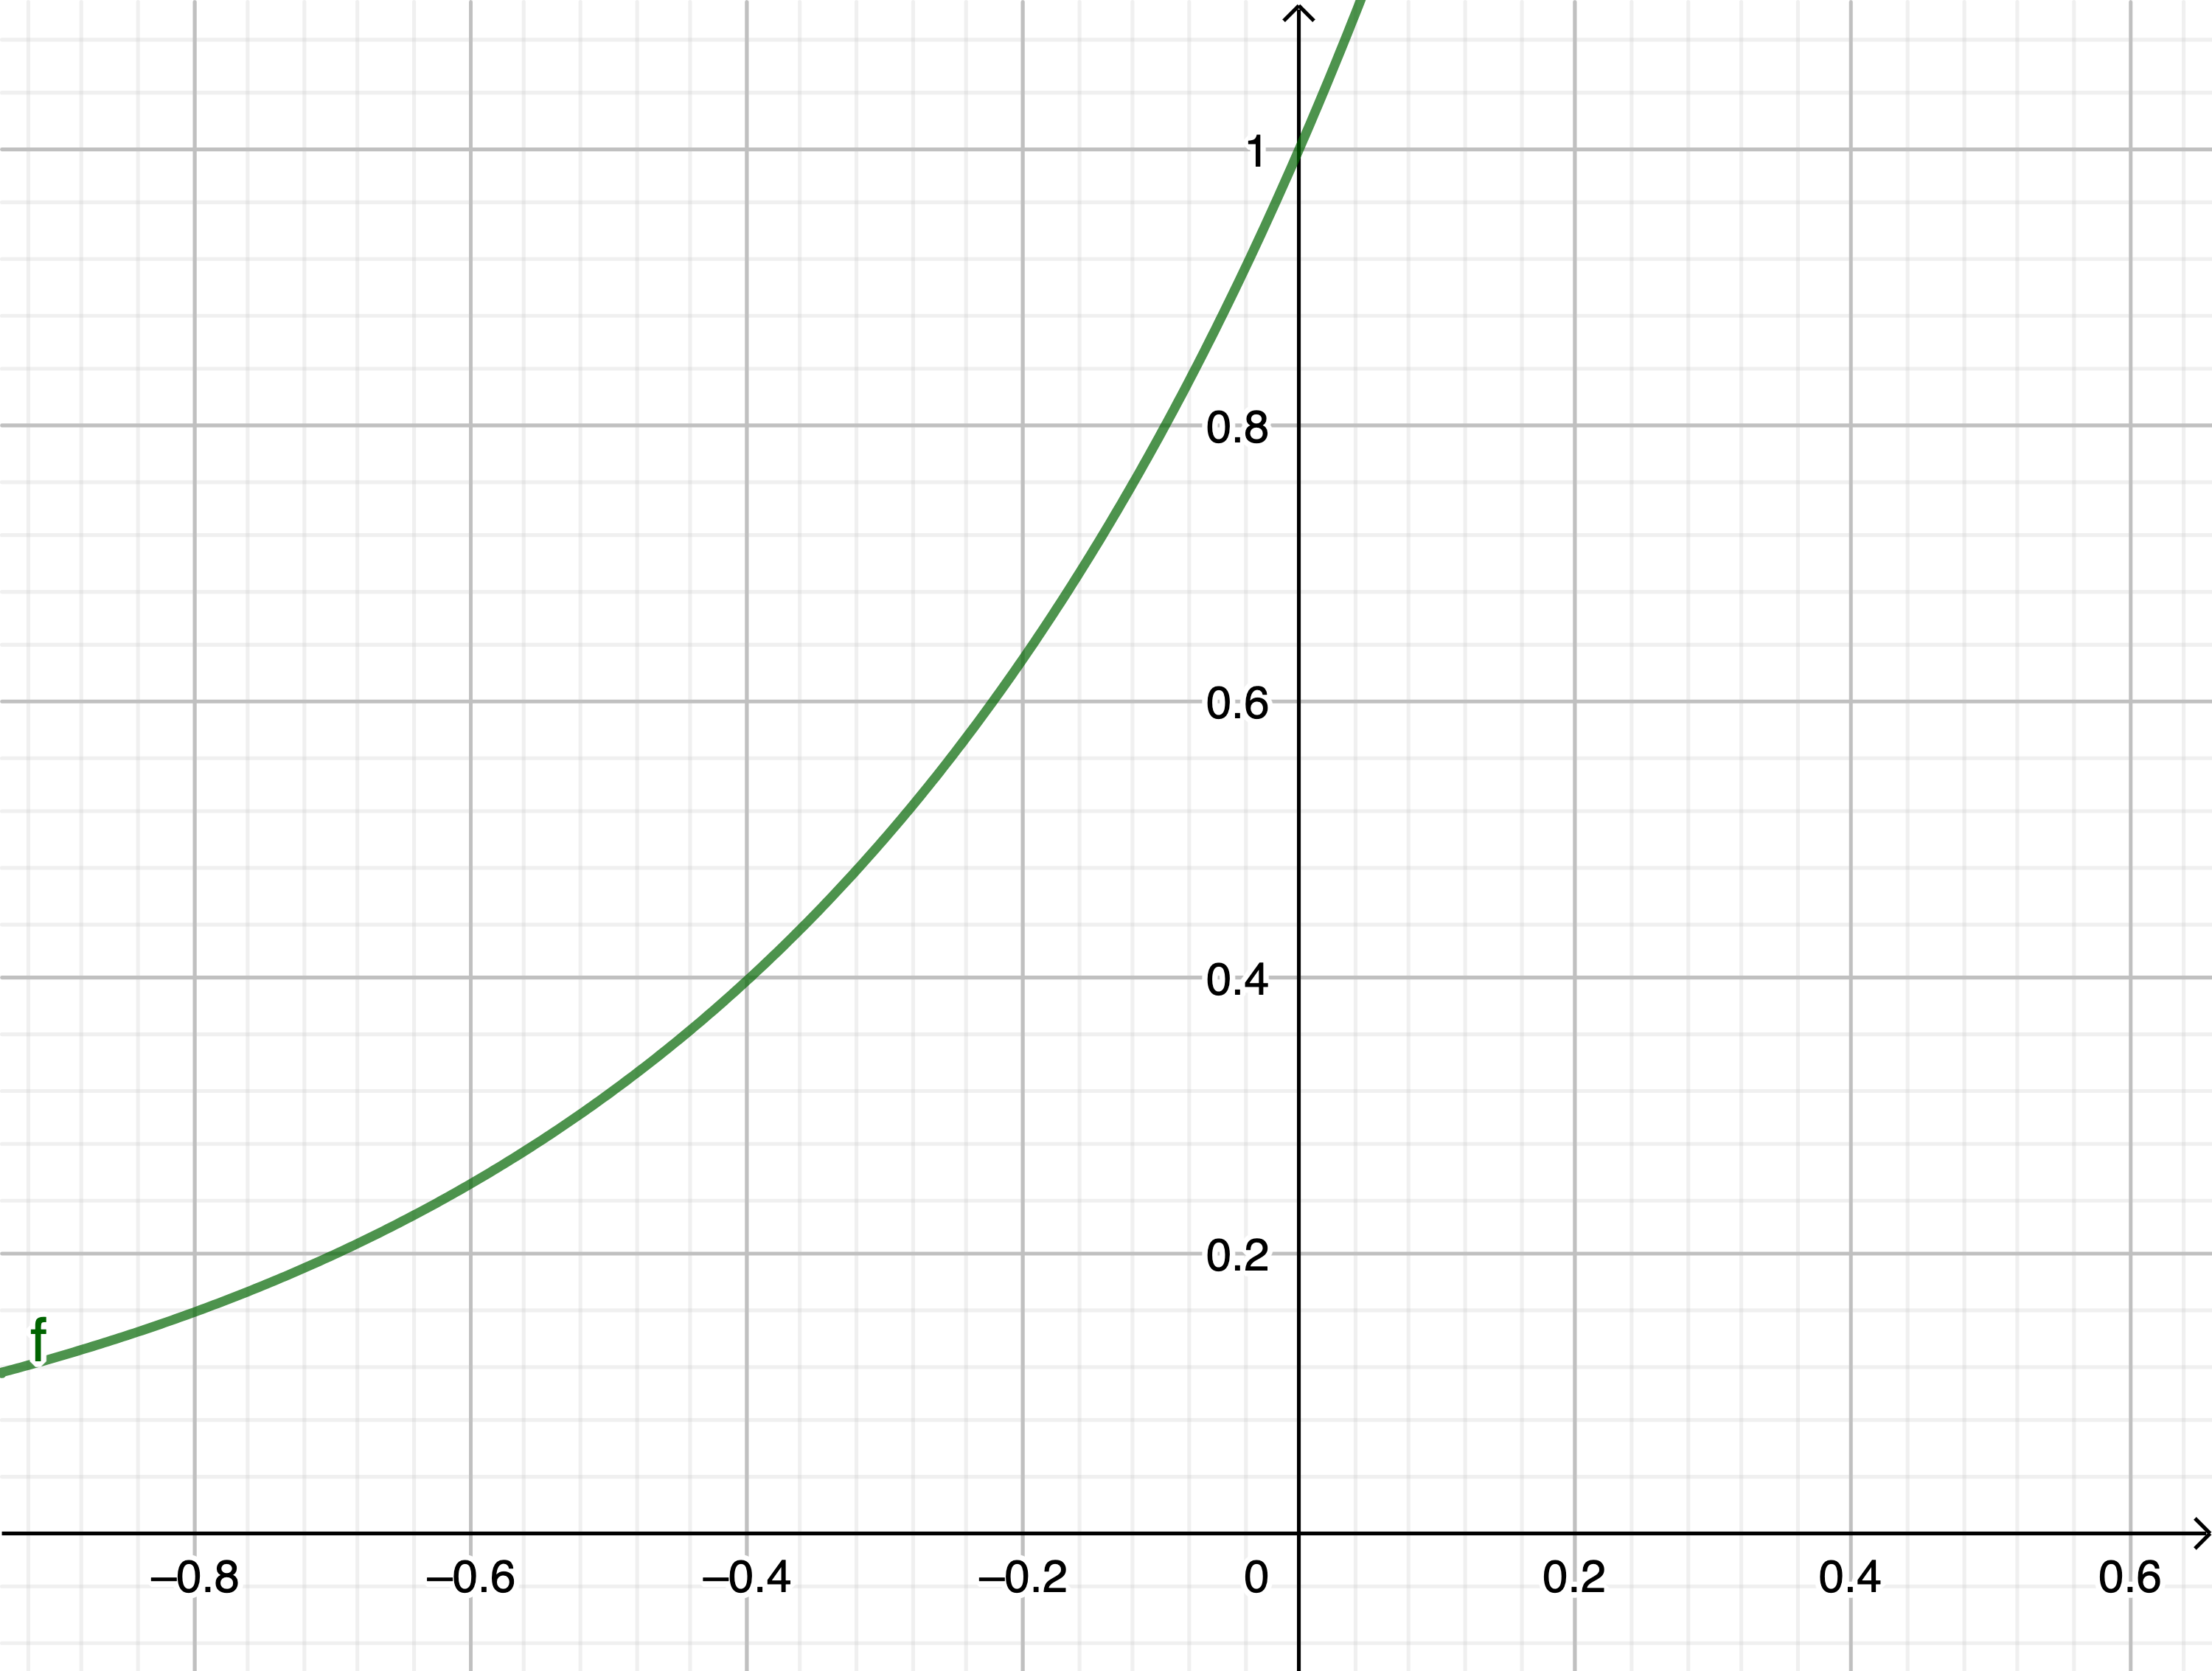
\includegraphics[scale=5]{media/Graph10hochx.png}
		      \end{center}
		\item 	Zeigen Sie mit dem Differenzialquotienten und einer Umformung: Die Funktion $f(x)=10^x$ hat die Ableitung
		      $$f'(x)=10^x\cdot \lim_{h\rightarrow0} \frac{10^h-1}{h} $$
		\item 	Füllen Sie die Tabelle aus und stützen Sie damit die Behauptung, dass die Ableitung von $f(x)=10^x$ wieder eine Exponentialfunktion ist, nämlich $f' (x)=c_{10}\cdot 10^x$ mit $c_{10}\approx 2.3026$.
		      \begin{center}

			      \begin{tabular}{c|c|c|c|c}

				      $h$                & $0.1$              & $0.01$             & $0.001$            & $0.0001$                                      \\ \hline
				      $\frac{10^h-1}{h}$ & $\phantom{2.3026}$ & $\phantom{2.3026}$ & $\phantom{2.3026}$ & $\phantom{2.3026}$\parbox[0pt][3em][c]{0cm}{}
			      \end{tabular}
		      \end{center}

		\item Gehen Sie gleich vor, um die Behauptung zu stützen, dass $\frac{d}{dx} 2^x = c_2\cdot 2^x$ mit $c_2\approx 0.693$.
		\item Halten wir fest: Die Ableitung von Exponentialfunktion der Form $y=a^x$ ist ein Vielfaches der Funktion selbst: $y'=c_a\cdot a^x$, wobei der Faktor $c_a$ von der gewählten Basis $a$ abhängig ist. Zum Beispiel ist $c_2 \approx 0.693$ und $c_{10} \approx 2.3026$.

		      Forschen: Finden Sie durch geschicktes Probieren eine Basis $a$, sodass der entsprechende Faktor $c_a \approx 1$ ist?
		      % \item Bestimmen Sie auf die gleiche Art, die Ableitung der Funktion $g(x)=e^x$, wobei $e = 2.7182818\cdots$ die Euler’sche Zahl ist. (Benutzen sie die entsprechende Taste für $e$ auf dem TR)
		      % \item 	Berechnen Sie den Logarithmus zur Basis $e$ von $10$ und von $2$ - also $\ln(10)$ und $\ln(2)$. Kommt Ihnen das Resultat bekannt vor? Ergänzen Sie die Vermutung unten:
		      % $$
		      % f(x)=a^x  \Longrightarrow f'(x)=\enspace\makebox[2in]{\hrulefill}
		      % $$

	\end{enumerate}

\end{LA}
\clearpage
Unter all den Exponentialfunktionen der Form $f(x)=a^x,a>0$ gibt es eine mit einer ganz besonderen Eigenschaft – jene, die als Basis die Eulersche Zahl $e$ hat. Für diese gilt nämlich

\begin{satz}
	{Die Ableitung der Exponentialfunktion zur Basis $e$}{}
	Die Funktion $f(x)=e^x$ ist überall differenzierbar und es gilt
	$$
		\frac{d}{dx} e^x = e^x
	$$
\end{satz}

\begin{proof}
	Die Eulersche Zahl $e=2.71828\cdots$ haben wir bereits bei der Zinseszins-Rechnung kennengelernt. Dort wurde sie definiert als den Grenzwert
	$$
		e= \lim_{n\rightarrow\infty} \left(1+\frac{1}{n}\right)^n
	$$
	Mit dem Differenzialquotienten folgt für die Ableitung der $e^x$-Funktion:
	$$
		\frac{d}{dx} e^x = \lim_{h\rightarrow0} \frac{e^{x+h}-e^x}{h} =  \lim_{h\rightarrow0} \frac{e^{x}\cdot e^h -e^x}{h} = e^x \cdot \lim_{h\rightarrow0} \frac{ e^h - 1}{h}
	$$
	Die Idee ist nun, dass man den Grenzwert $\lim_{h\rightarrow0} \frac{ e^h - 1}{h}$ so umformt, dass die Definition von $e= \lim_{n\rightarrow\infty} \left(1+\frac{1}{n}\right)^n$ darin vorkommt. Dazu ersetzen wir die Variable $h$ durch $h=\ln\left(1+\frac{1}{n}\right) $, wobei $n$ eine positive reelle Zahl ist, die gegen Unendlich strebt, wenn $h$ gegen Null strebt. Die Ableitung der $e$-Funktion lautet nun
	\begin{align*}
		\frac{d}{dx} e^x & =  e^x \cdot \lim_{n\rightarrow\infty} \frac{ e^{\ln\left(1+\frac{1}{n}\right)} - 1}{\ln\left(1+\frac{1}{n}\right)}        \\
		                 & = e^x \cdot \lim_{n\rightarrow\infty} \frac{1+\frac{1}{n}-1}{\ln\left(1+\frac{1}{n}\right)}                                \\
		                 & = e^x \cdot \lim_{n\rightarrow\infty} \frac{1}{n\cdot \ln\left(1+\frac{1}{n}\right)}                                       \\
		                 & \stackrel{\text{Log-Gesetz}}{=} e^x \cdot \lim_{n\rightarrow\infty} \frac{1}{\ln\left[\left(1+\frac{1}{n}\right)^n\right]} \\
		                 & \stackrel{\text{Def von }e}{=}  e^x \cdot  \frac{1}{\ln(e)}                                                                \\
		                 & = e^x
	\end{align*}
\end{proof}
Die Ableitungen von Exponentialfunktionen mit einer anderen Basis lassen sich leicht auf die $e^x$-Funktion zurückführen. Es gilt
\begin{satz}
	{Die Ableitung allgemeiner Exponentialfunktionen}{}
	Sei $f(x)=a^x$ mit $a>0$. Dann ist $f$ überall differenzierbar und es gilt
	$$
		f'(x)= \ln(a) \cdot a^x
	$$

\end{satz}
\begin{proof}
	$$f(x)=a^x = \left(e^{\ln(a)}\right)^x = e^{\ln(a)\cdot x} $$
	Mit der Kettenregel folgt dann:
	$$f'(x)= \underbrace{e^{\ln(a)\cdot x}}_{\text{äussere Ableitung}} \cdot \underbrace{\ln(a)}_{\text{innere Ableitung}} = a^x \cdot \ln(a)
	$$

\end{proof}

\begin{ueb}
	{}{}
	\begin{enumerate}
		\item Bestimme die Ableitung der folgenden Funktionen:
		      \begin{enumerate}
			      \item $y= 42\cdot e^x$
			      \item $y= e^{5x}$
			      \item $y= x\cdot e^x$
			      \item $y= x^2 \cdot e^{-x}$
			      \item $y= \frac{e^x}{x^2+1}$
			      \item $y= e^{\sin(x)}$
			      \item $y = \frac{e^x+e^{-x}}{2}$ (Diese Funktion heisst auch \emph{Cosinus-Hyperbolicus} und wird mit $\cosh(x)$ bezeichnet.)
		      \end{enumerate}
		\item In welchem Kurvenpunkt hat die Funktion $f(x) = e^{2x}$ eine Tangente mit der Steigung $m=8$? Bestimme die Koordinaten des Punktes.
		\item \emph{Challenge:} Der Graph der Funktion $f(x) = e^x$ sowie ein beliebiger Kurvenpunkt $P=(u,v)$ sind gegeben. In $P$ werden die Kurventangente $t$ sowie eine Parallele $s$ zur $y$-Achse eingezeichnet. Seien $S$ und $T$ die Schnittpunkte der beiden Geraden mit der $x$-Achse.
		      \begin{enumerate}
			      \item Berechne den Abstand zwischen den Punkten $S$ und $T$.
			      \item Bestimme $u$ so, dass die Tangente $t$ durch den Ursprung verläuft.
			      \item Bestimme $u$ so, dass das Dreieck $STP$ den Flächeninhalt $A=e$ hat.
		      \end{enumerate}
	\end{enumerate}
\end{ueb}
\clearpage
\emph{Lösungen:}
\begin{enumerate}
	\item
	      \begin{enumerate}
		      \item $y'= 42\cdot e^x$
		      \item $y'= 5e^{5x}$
		      \item $y'= e^x + x\cdot e^x$
		      \item $y'= 2x\cdot e^{-x} - x^2 \cdot e^{-x}$
		      \item $y' = \frac{(x^2+1)e^x-2xe^x}{(x^2+1)^2}$
		      \item $y' = \cos(x) \cdot e^{\sin(x)}$
		      \item $y' = \frac{e^x-e^{-x}}{2}$ (Diese Funktion heisst auch \emph{Sinus-Hyperbolicus} und wird mit $\sinh(x)$ bezeichnet.)
	      \end{enumerate}
	\item $B=(\ln(2), 4)$ (Hinweis: $\ln(2)$ ist wegen der Logarithmusgesetze das gleiche wie $\frac{\ln(4)}{2}$)

	\item
	      \begin{enumerate}
		      \item Der Abstand ist immer $1$. (Zwischenresultat: Die Gleichung der Tangente in $P$ lautet $t: \, y = e^u \cdot x + e^u - u\cdot e^u$)
		      \item $u=1$
		      \item $u = \ln(2e) = 1+\ln(2)$
	      \end{enumerate}
\end{enumerate}


































\pagebreak

\subsubsection{Die Ableitung von Umkehrfunktionen}
\begin{LA}
	{Spieglein, Spieglein im ersten Quadrant}{}
	In dieser Lernaufgabe werden Sie den Zusammenhang zwischen den Ableitungen von Funktionen ergründen, die Umkehrfunktionen voneinander sind.

	% Zur Erinnerung: Zu jeder bijektiven Funktion $f$ gibt es eine Umkehrfunktion $f^{-1}$ mit der Eigenschaft, dass
	% $$f^{-1}(f(x)) = f(f^{-1}(x)) = x$$
	% Die Graphen von $f$ und von $f^{-1}$ sind spiegelsymmetrisch bezüglich der Winkelhalbierenden des 1. und 3. Quadranten. Damit lässt sich der Zusammenhang zwischen den Ableitungen durch geometrische Überlegungen finden.

	\begin{enumerate}
		\item Betrachten wir als erstes die Wurzelfunktionen. Deren Ableitung haben wir schon mit dem Differentialquotienten hergeleitet. In dieser Aufgabe wollen wir die Ableitung der Wurzelfunktion noch einmal auf einem anderen Weg finden, indem wir sie als Umkehrfunktion der Quadratfunktion betrachten. Sei also $f(x)= \sqrt{x}$ und $g(x) = f^{-1}(x)=x^2$ (mit $x\ge0$).
		      \begin{center}
			      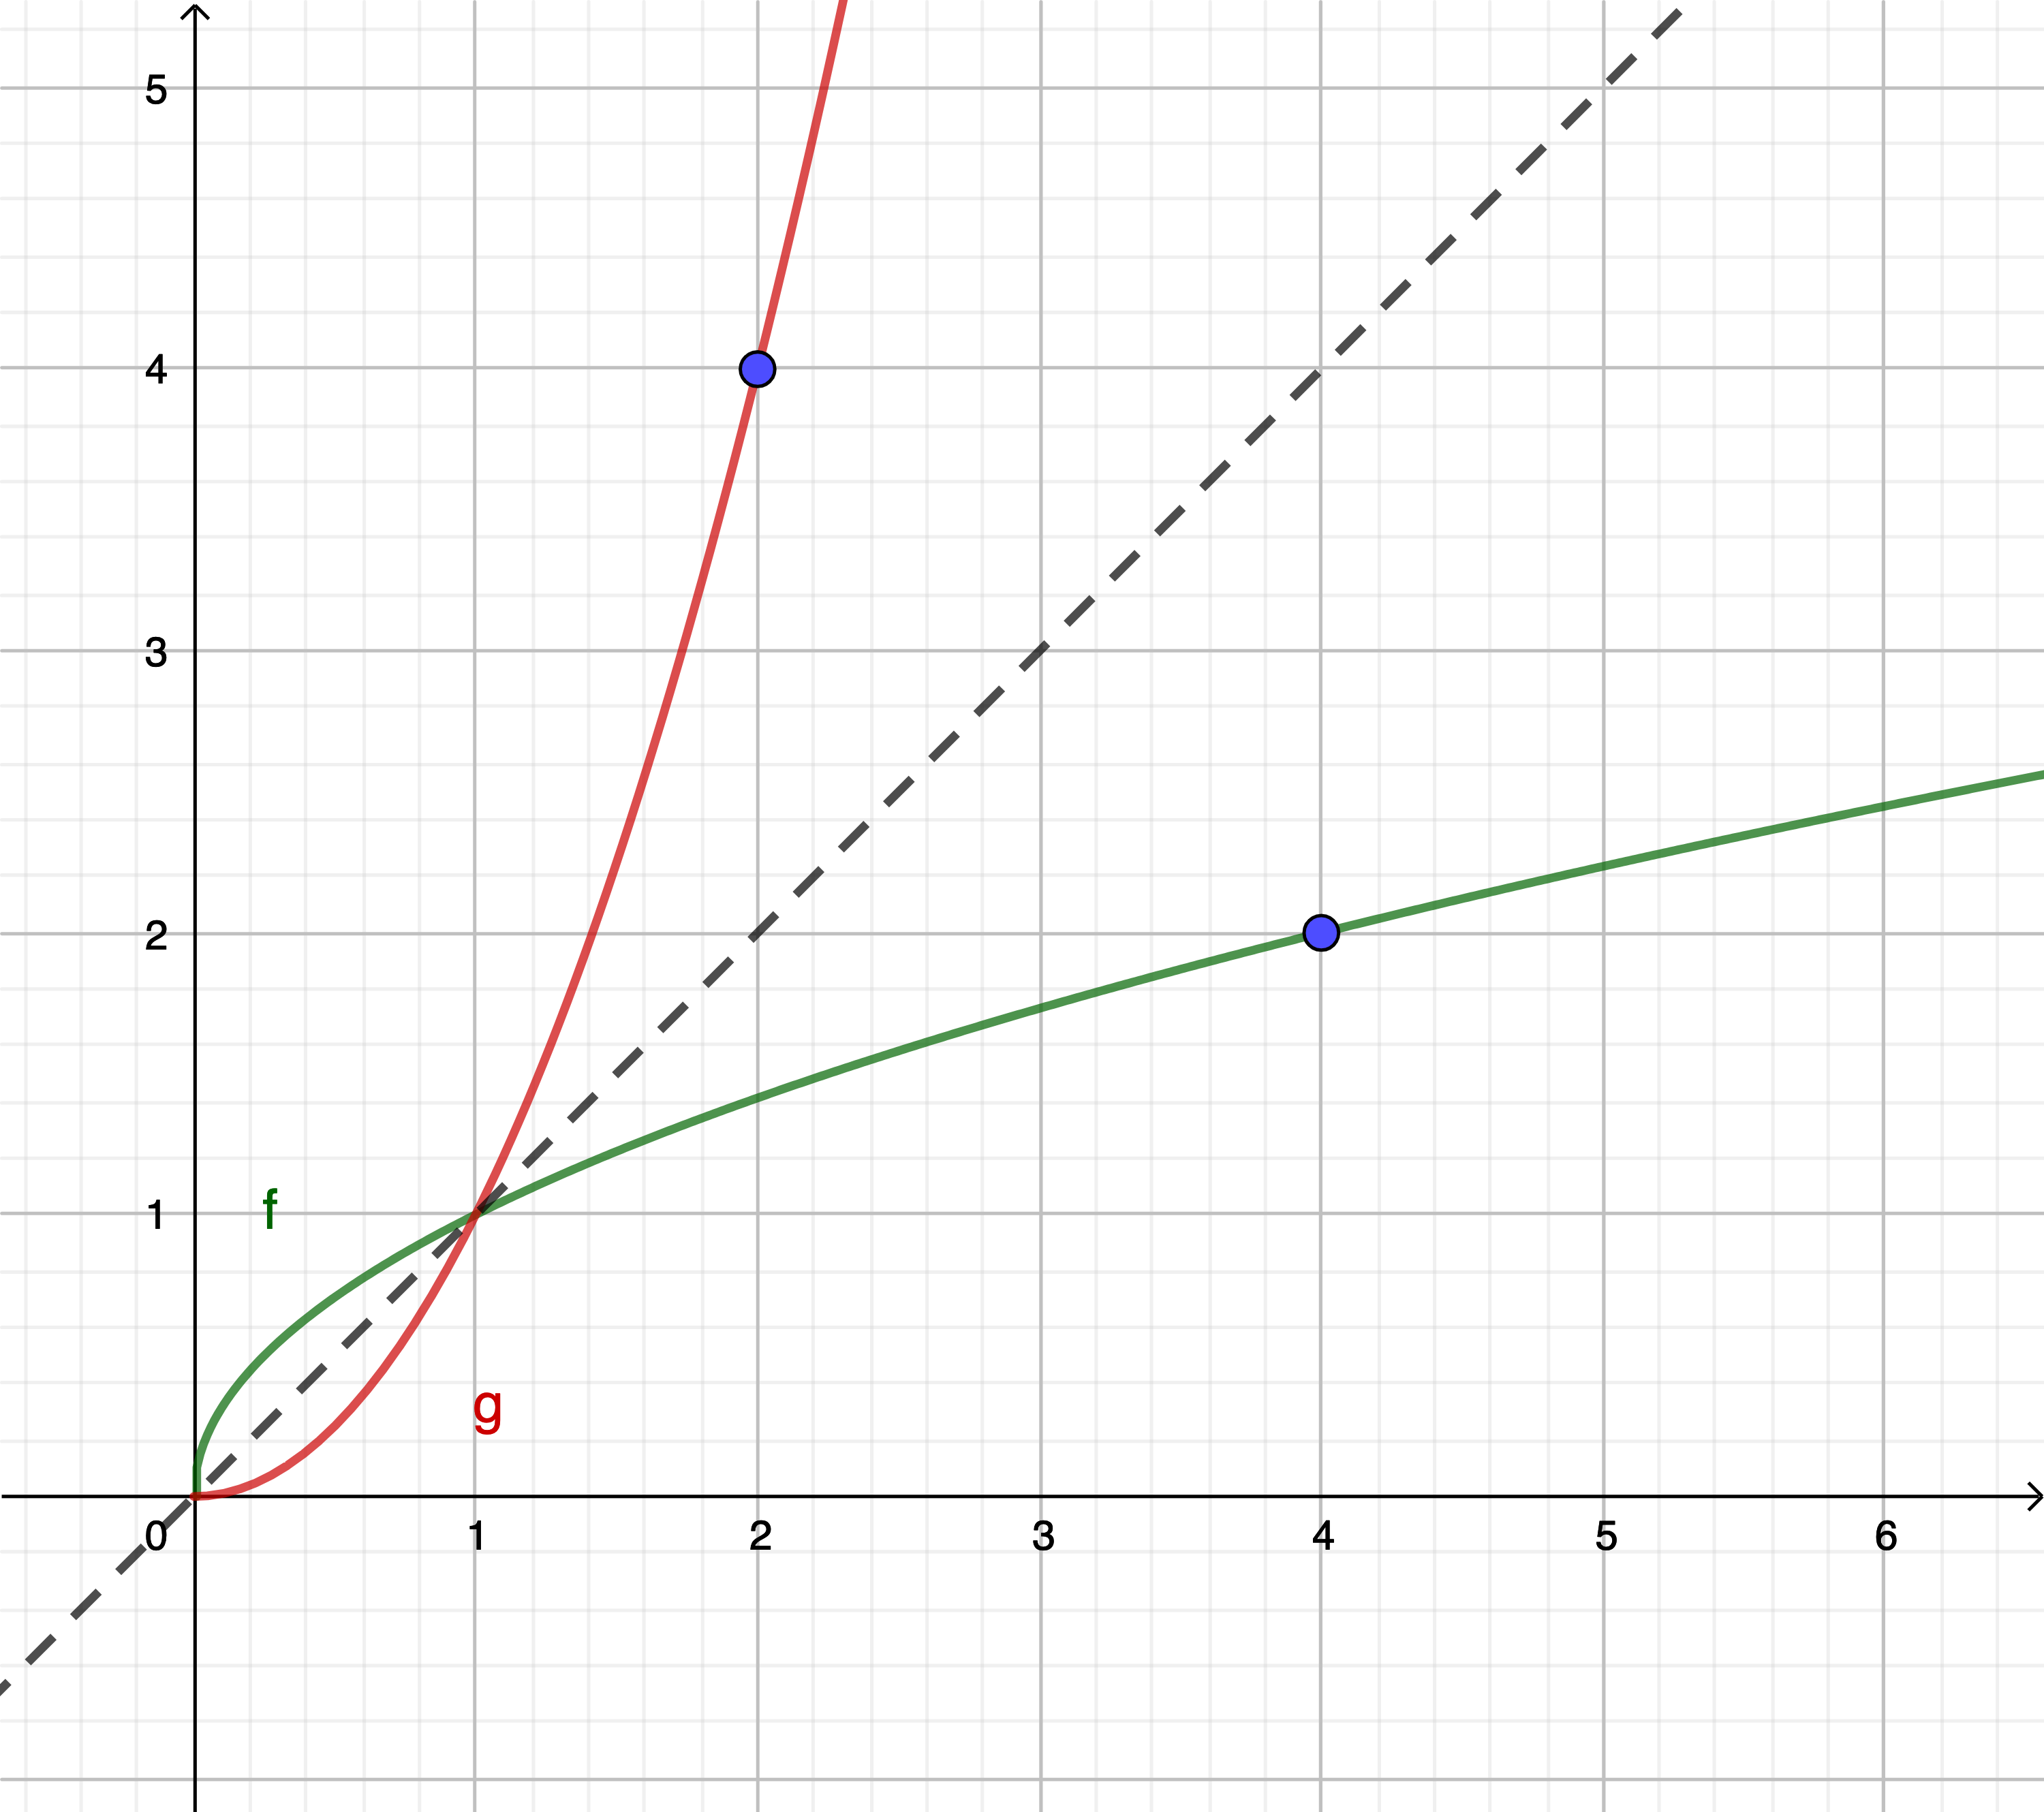
\includegraphics[scale=1.5]{media/spiegleinspieglein.png}
		      \end{center}
		      Die Tatsache, dass die Graphen symmetrisch bezüglich der Winkelhalbbierenden verlaufen, können wir ausnutzen, um die Ableitung der Wurzelfunktion zu finden.
		      \begin{enumerate}
			      \item 	Zeichnen Sie die Tangenten an die Graphen in den Punkten $(4|2)$ bzw. $(2|4)$ ein.
			      \item Erklären Sie: Wieso entspricht die Steigung der einen Tangente dem Kehrwert der Steigung der anderen Tangente?
			      \item Berechnen Sie die Steigung $g'(2)$ (mit der üblichen Regel für Potenzen). Was ist demnach $f'(4)$?
			      \item Zeigen Sie auf die gleiche Weise, dass $f' (9)=\frac{1}{6}$ ist.
			      \item Erklären Sie, wie man auf diese Weise die Ableitung $f'(x)=\frac{1}{2\sqrt{x}}$ finden kann.
		      \end{enumerate}
	\end{enumerate}

	Die Idee aus Aufgabe 1 kann auch auf andere Paare von Funktion und Umkehrfunktion übertragen werden:
	\begin{enumerate}[resume]
		\item Wir betrachten als nächstes die Exponentialfunktion und den Logarithmus zur Basis $e$:
		      \begin{center}
			      \begin{center}
				      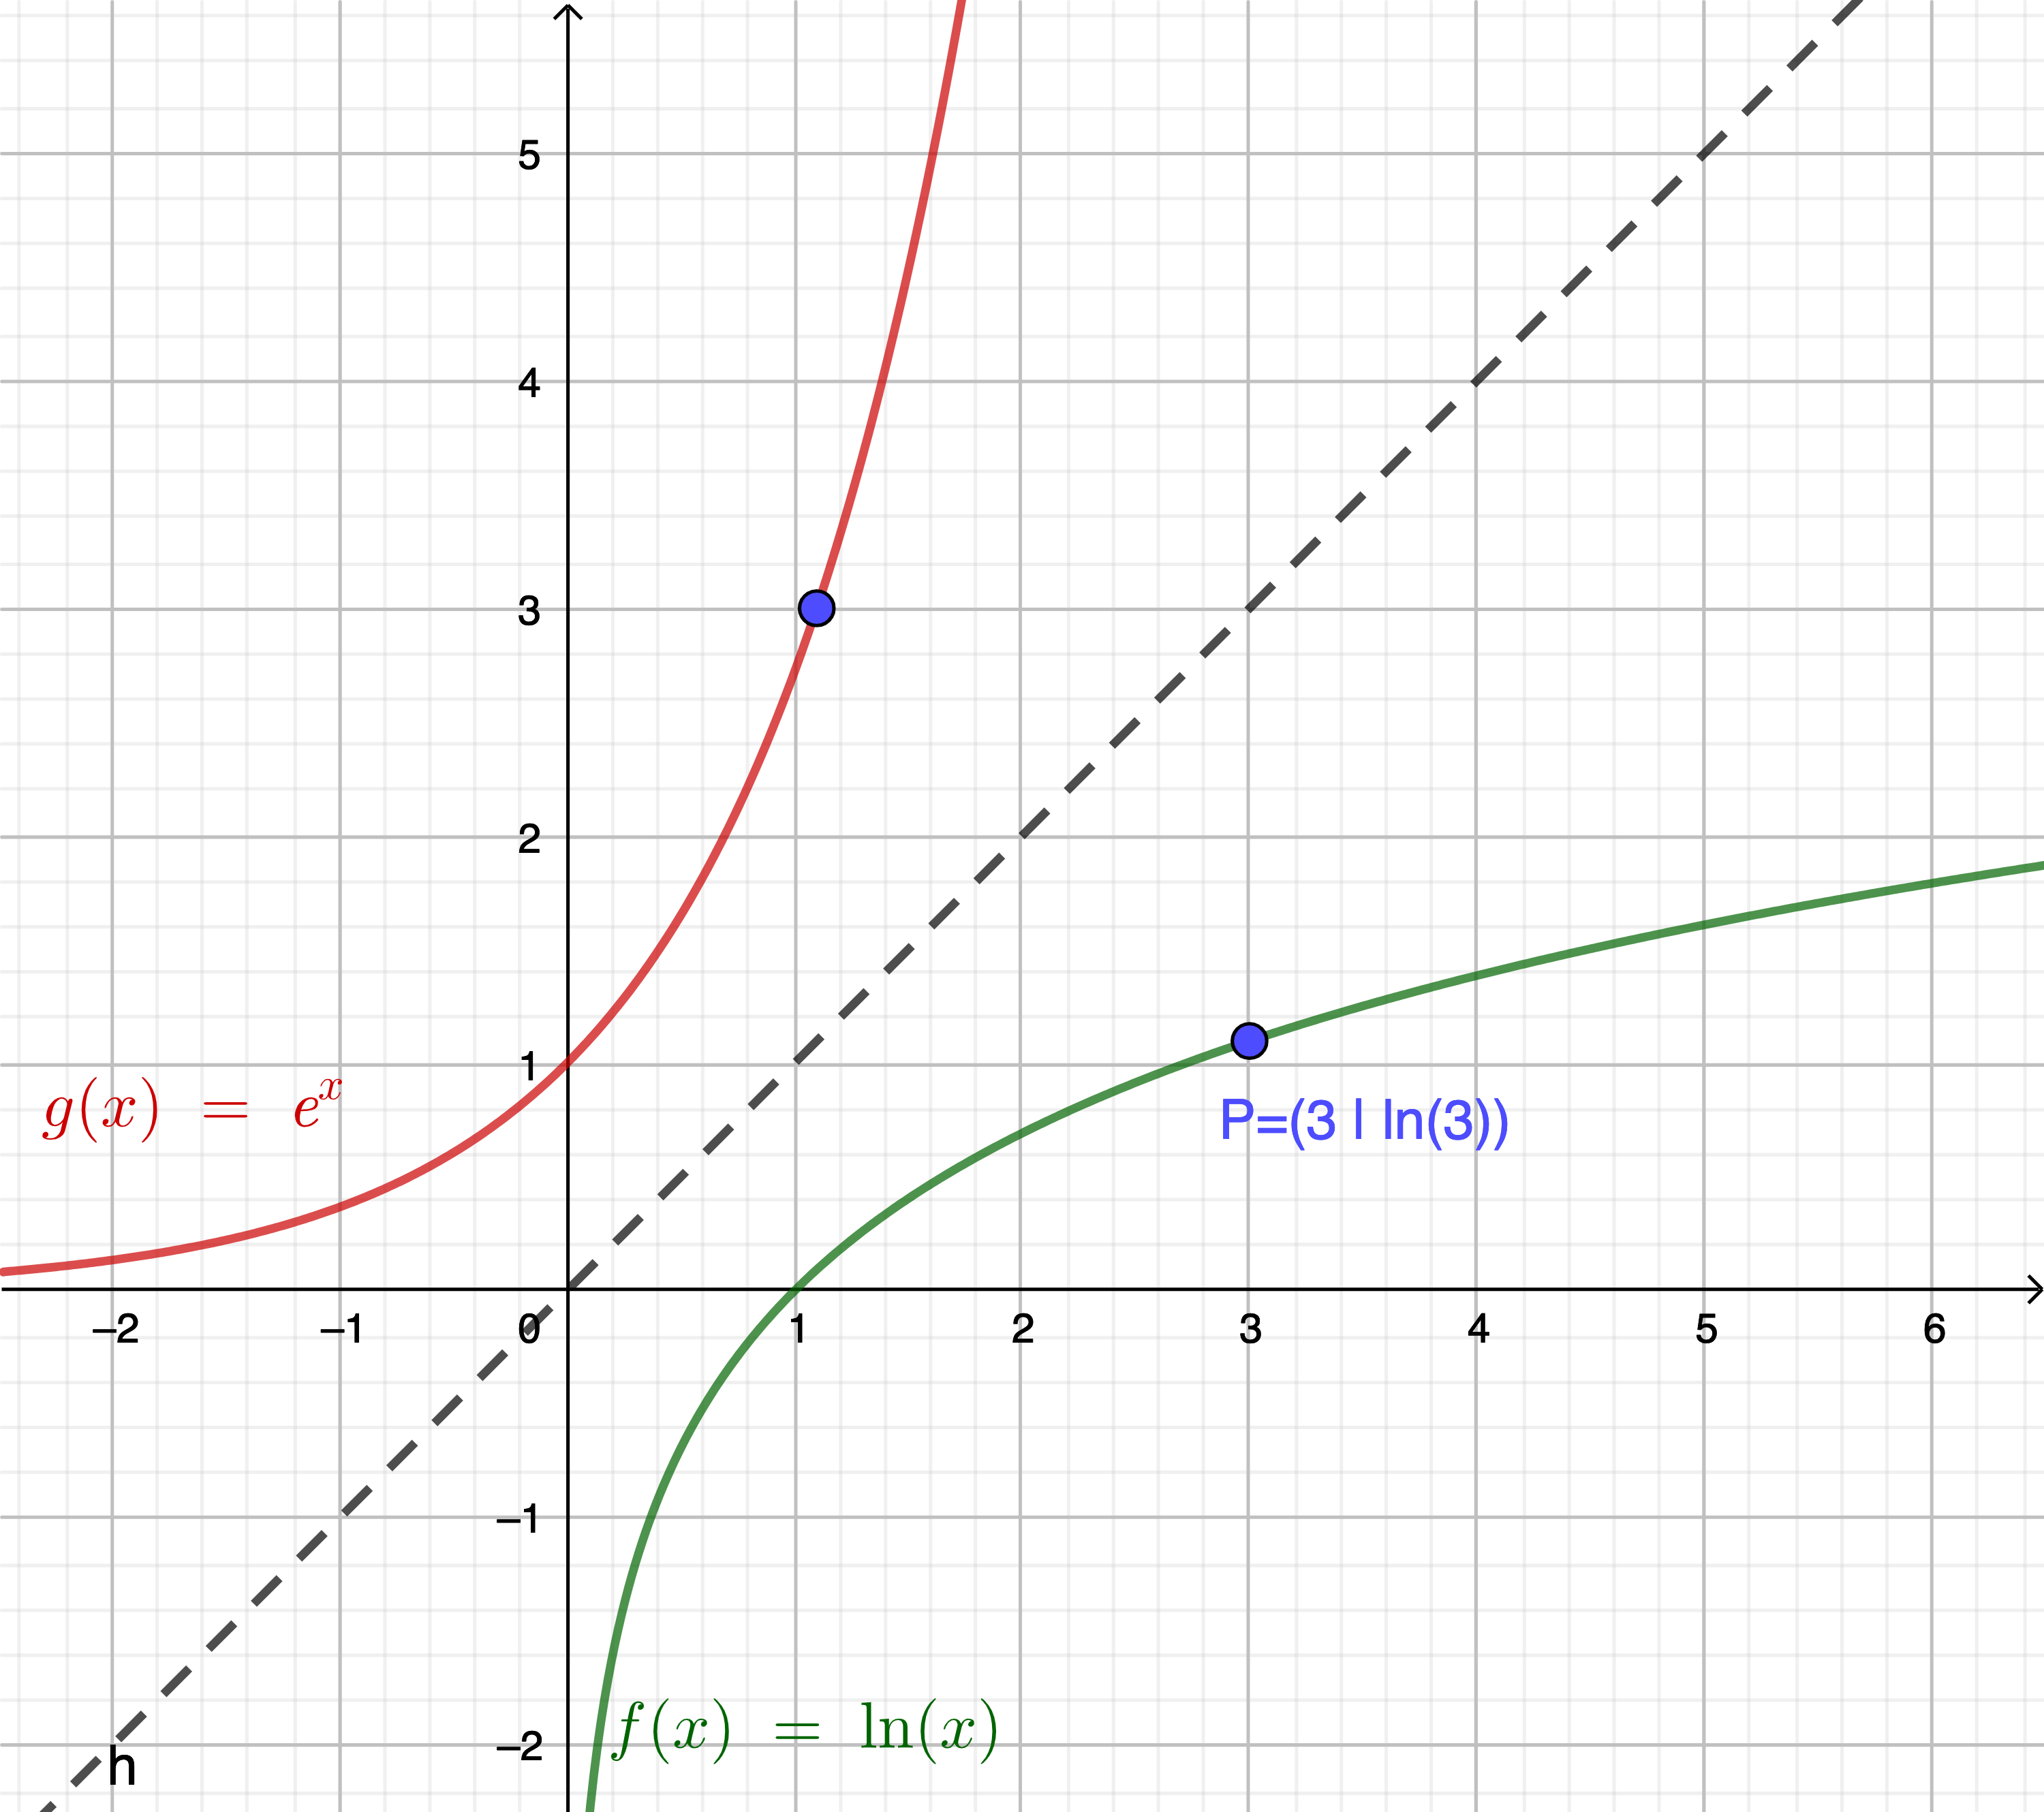
\includegraphics[scale=1.5]{media/spiegleinspiegleinMitLn.png}
			      \end{center}
		      \end{center}
		      \begin{enumerate}
			      \item Berechnen Sie $\ln'(3)$. Nutzen Sie dazu die in der Skizze eingezeichneten Punkte und die Ableitungsregel für die Funktion $g(x)=e^x$
			      \item Geben Sie allgemein die Gleichung von $\ln'(x)$ an.
		      \end{enumerate}
		\item Challenge 1: Die Beziehung zwischen der Ableitung einer Funktion $f$ und jener ihrer Umkehrfunktion $g=f^{-1}$ kann auch als Formel angeben werden:
		      \begin{enumerate}
			      \item Führen Sie die Überlegungen aus den Aufgaben 1 und 2 allgemein durch und geben Sie eine Formel an, mit der man die Ableitung einer Funktion $f$ aus der Ableitung ihrer Umkehrfunktion $g=f^{-1}$ berechnen kann.
			      \item Die Formel aus Aufgabe (a) kann auch mit der Kettenregel hergeleitet werden. Leiten Sie dazu beide Seiten der Gleichung $g(f(x)) = x$ ab und lösen Sie die erhalten Gleichung nach $f'(x)$ auf.
		      \end{enumerate}
		\item Challenge 2: Beweisen Sie mit der Formel aus Aufgabe 3
		      $$ \arcsin'(x) = \frac{1}{\sqrt{1-x^2}}$$

	\end{enumerate}


\end{LA}


Die Ergebnisse der Lernaufgabe lassen sich wie folgt Zusammenfassen:
\begin{satz}
	{Ableitung von Umkehrfunktionen}{}
	Sei $f: ]a,b[\rightarrow\mathbb{W}$ eine bijektive, differenzierbare Funktion und sei $g=f^{-1}$ ihre Umkehrfunktion. Dann gilt:
	$$f'(x) = \frac{1}{g'(f(x))}$$
	Insbesondere folgen daraus die Ableitungsregeln:
	\begin{align*}
		\ln'(x)     & = \frac{1}{x}              \\
		\log'_a(x)  & = \frac{1}{x\cdot \ln(a)}  \\
		\arcsin'(x) & = \frac{1}{\sqrt{1-x^2}}   \\
		\arccos'(x) & = - \frac{1}{\sqrt{1-x^2}} \\
		\arctan'(x) & = \frac{1}{1+x^2}          \\
	\end{align*}
\end{satz}

\begin{proof}
	Für die Funktionen $f$ und $g=f^{-1}$ gilt:
	$$ g(f(x)) = x$$
	Wenn man nun beide Seiten der Gleichung nach $x$ ableiten, erhält man mit der Kettenregel:
	$$ g'(f(x)) \cdot f'(x) = 1$$
	Auflösen nach $f'(x)$ liefert dann die Aussage des Satzes:
	$$f'(x) = \frac{1}{g'(f(x))}$$
\end{proof}

\clearpage
\begin{ueb}
	{}{}
	\begin{enumerate}
		\item Bestimme die Ableitung der folgenden Funktionen:
		      \begin{enumerate}
			      \item $y= x^2 \cdot \ln(x)$
			      \item $y= \ln(2-3x)$
			      \item $y=\ln(\cos(x))$
			      \item $y= \ln\left(\frac{x}{x+1}\right)$


		      \end{enumerate}
		\item Bestimme die Ableitung der Funktion $f(x) = \ln(2x)$. Erkläre das überraschende Resultat mit dem Logarithmusgesetz $\ln(a\cdot b) = \ln(a) + \ln(b)$.
		\item Bestimme die Gleichung der Tangente, welche die Kurve $y=e^x\cdot \ln(x)$ in deren Nullstelle berührt.
	\end{enumerate}
\end{ueb}

\clearpage
\emph{Lösungen:}
\begin{enumerate}
	\item
	      \begin{enumerate}
		      \item $y' = 2x \ln(x) + x$
		      \item $y'= \frac{-3}{2-3x}$
		      \item $y'= -\tan(x)$
		      \item $y'= \frac{1}{x^2+1}$


	      \end{enumerate}
	\item $f'(x) = \frac{1}{x}$
	\item Nullstelle bei $x=1$, Tangente: $y= ex-e$
\end{enumerate}







































\clearpage
\subsubsection{Höhere Ableitungen}
\begin{LA}
	{Von der Ableitung zum Funktionsgraphen}{}
	\begin{enumerate}
		\item Skizzieren Sie den Graphen der quadratischen Funktion $f(x)=12x^2-24x$. Sie müssen nicht allzu präzise sein, der grobe Verlauf und die Nullstellen reichen aus.
		      % \begin{center}
		      %     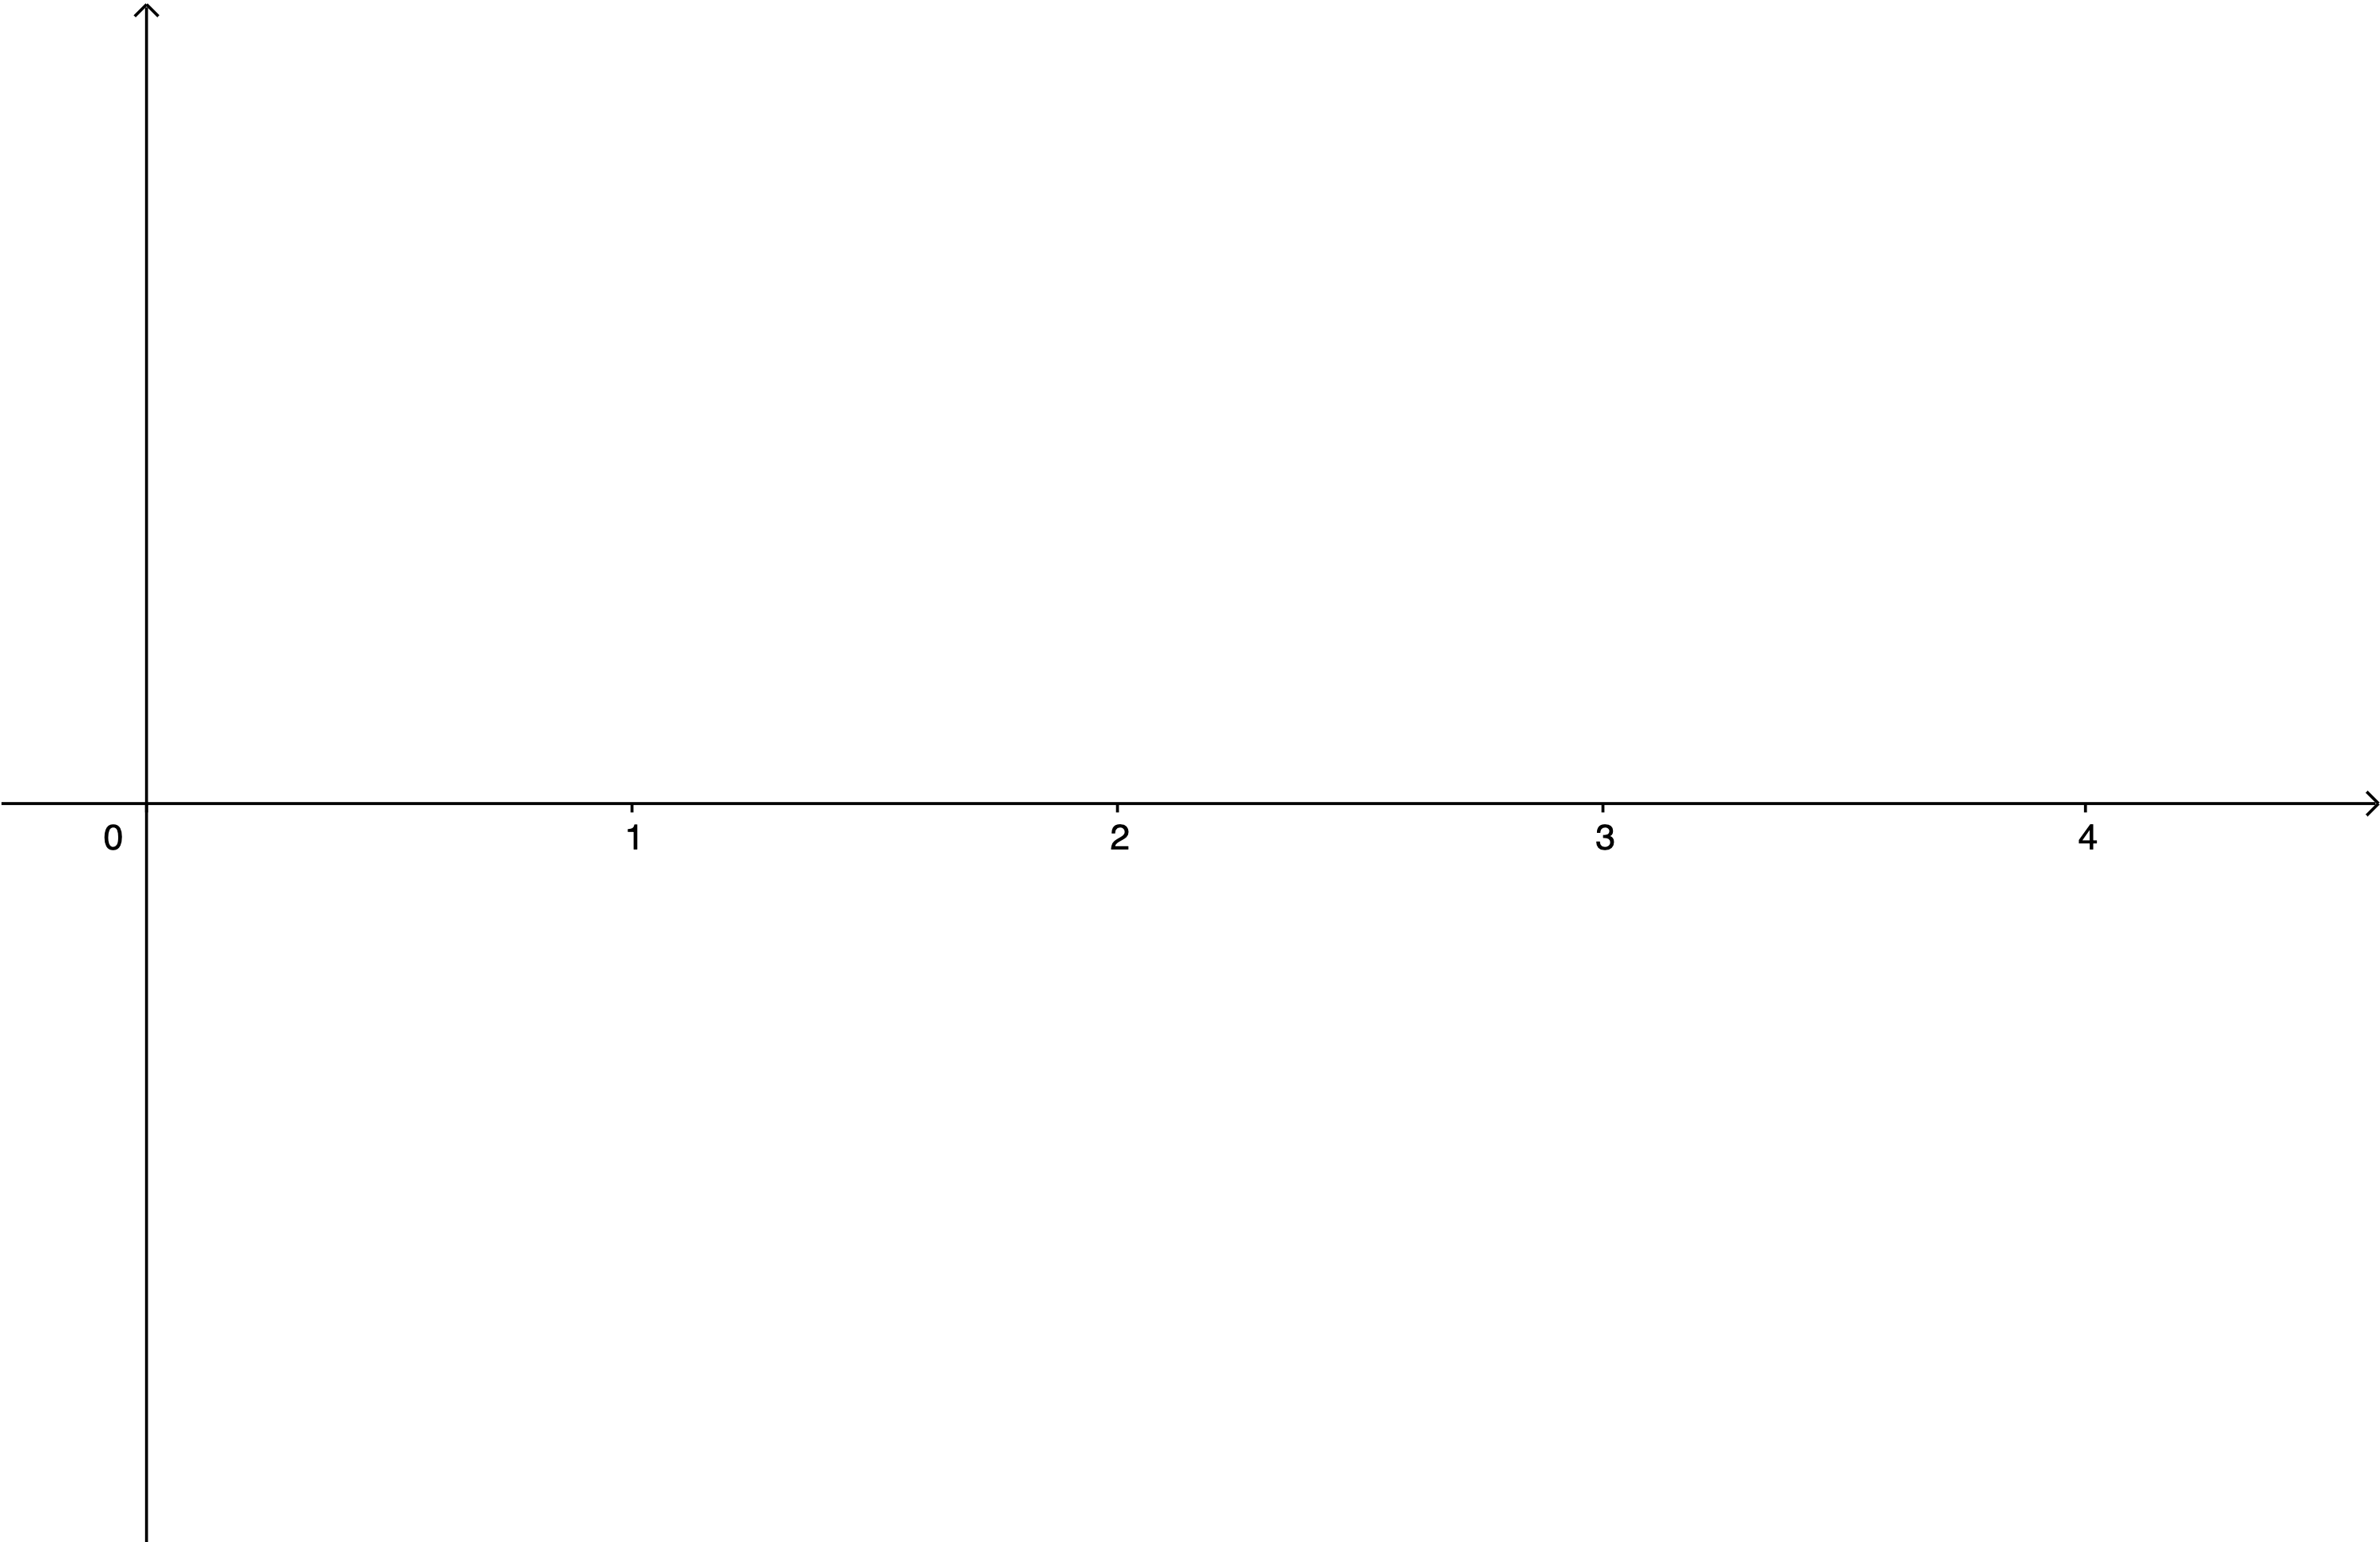
\includegraphics[scale=1.5]{media/KS-hoereAbleitung.png}
		      % \end{center}

		      \begin{center}
			      \begin{tikzpicture}
				      % Achsen
				      \draw[->, thick] (-1,0) -- (9,0) node[right] {$x$};
				      \draw[->, thick] (0,-3) -- (0,3) node[above] {$y$};

				      % Beschriftungen der Achsen
				      \foreach \x in {1,2,3,4} {
						      \draw (2*\x,-0.1) -- (2*\x,0.1);
						      \node[below] at (2*\x,-0.1) {\x };
					      }
			      \end{tikzpicture}
		      \end{center}

		\item Betrachten Sie nun die Funktion $g(x)=4x^3-12x^2$. Auch von dieser Funktion soll eine ungefähre Skizze gefertigt werden. Dies ist jedoch nicht mehr so einfach, schliesslich es ist keine quadratische Funktion! Jedoch gilt: $g'(x)=f(x)$. Nutzen Sie diese Information, um den Graphen von $g$ ungefähr zu skizzieren. Berechnen Sie die Nullstellen wieder exakt.
		      % \begin{center}
		      %     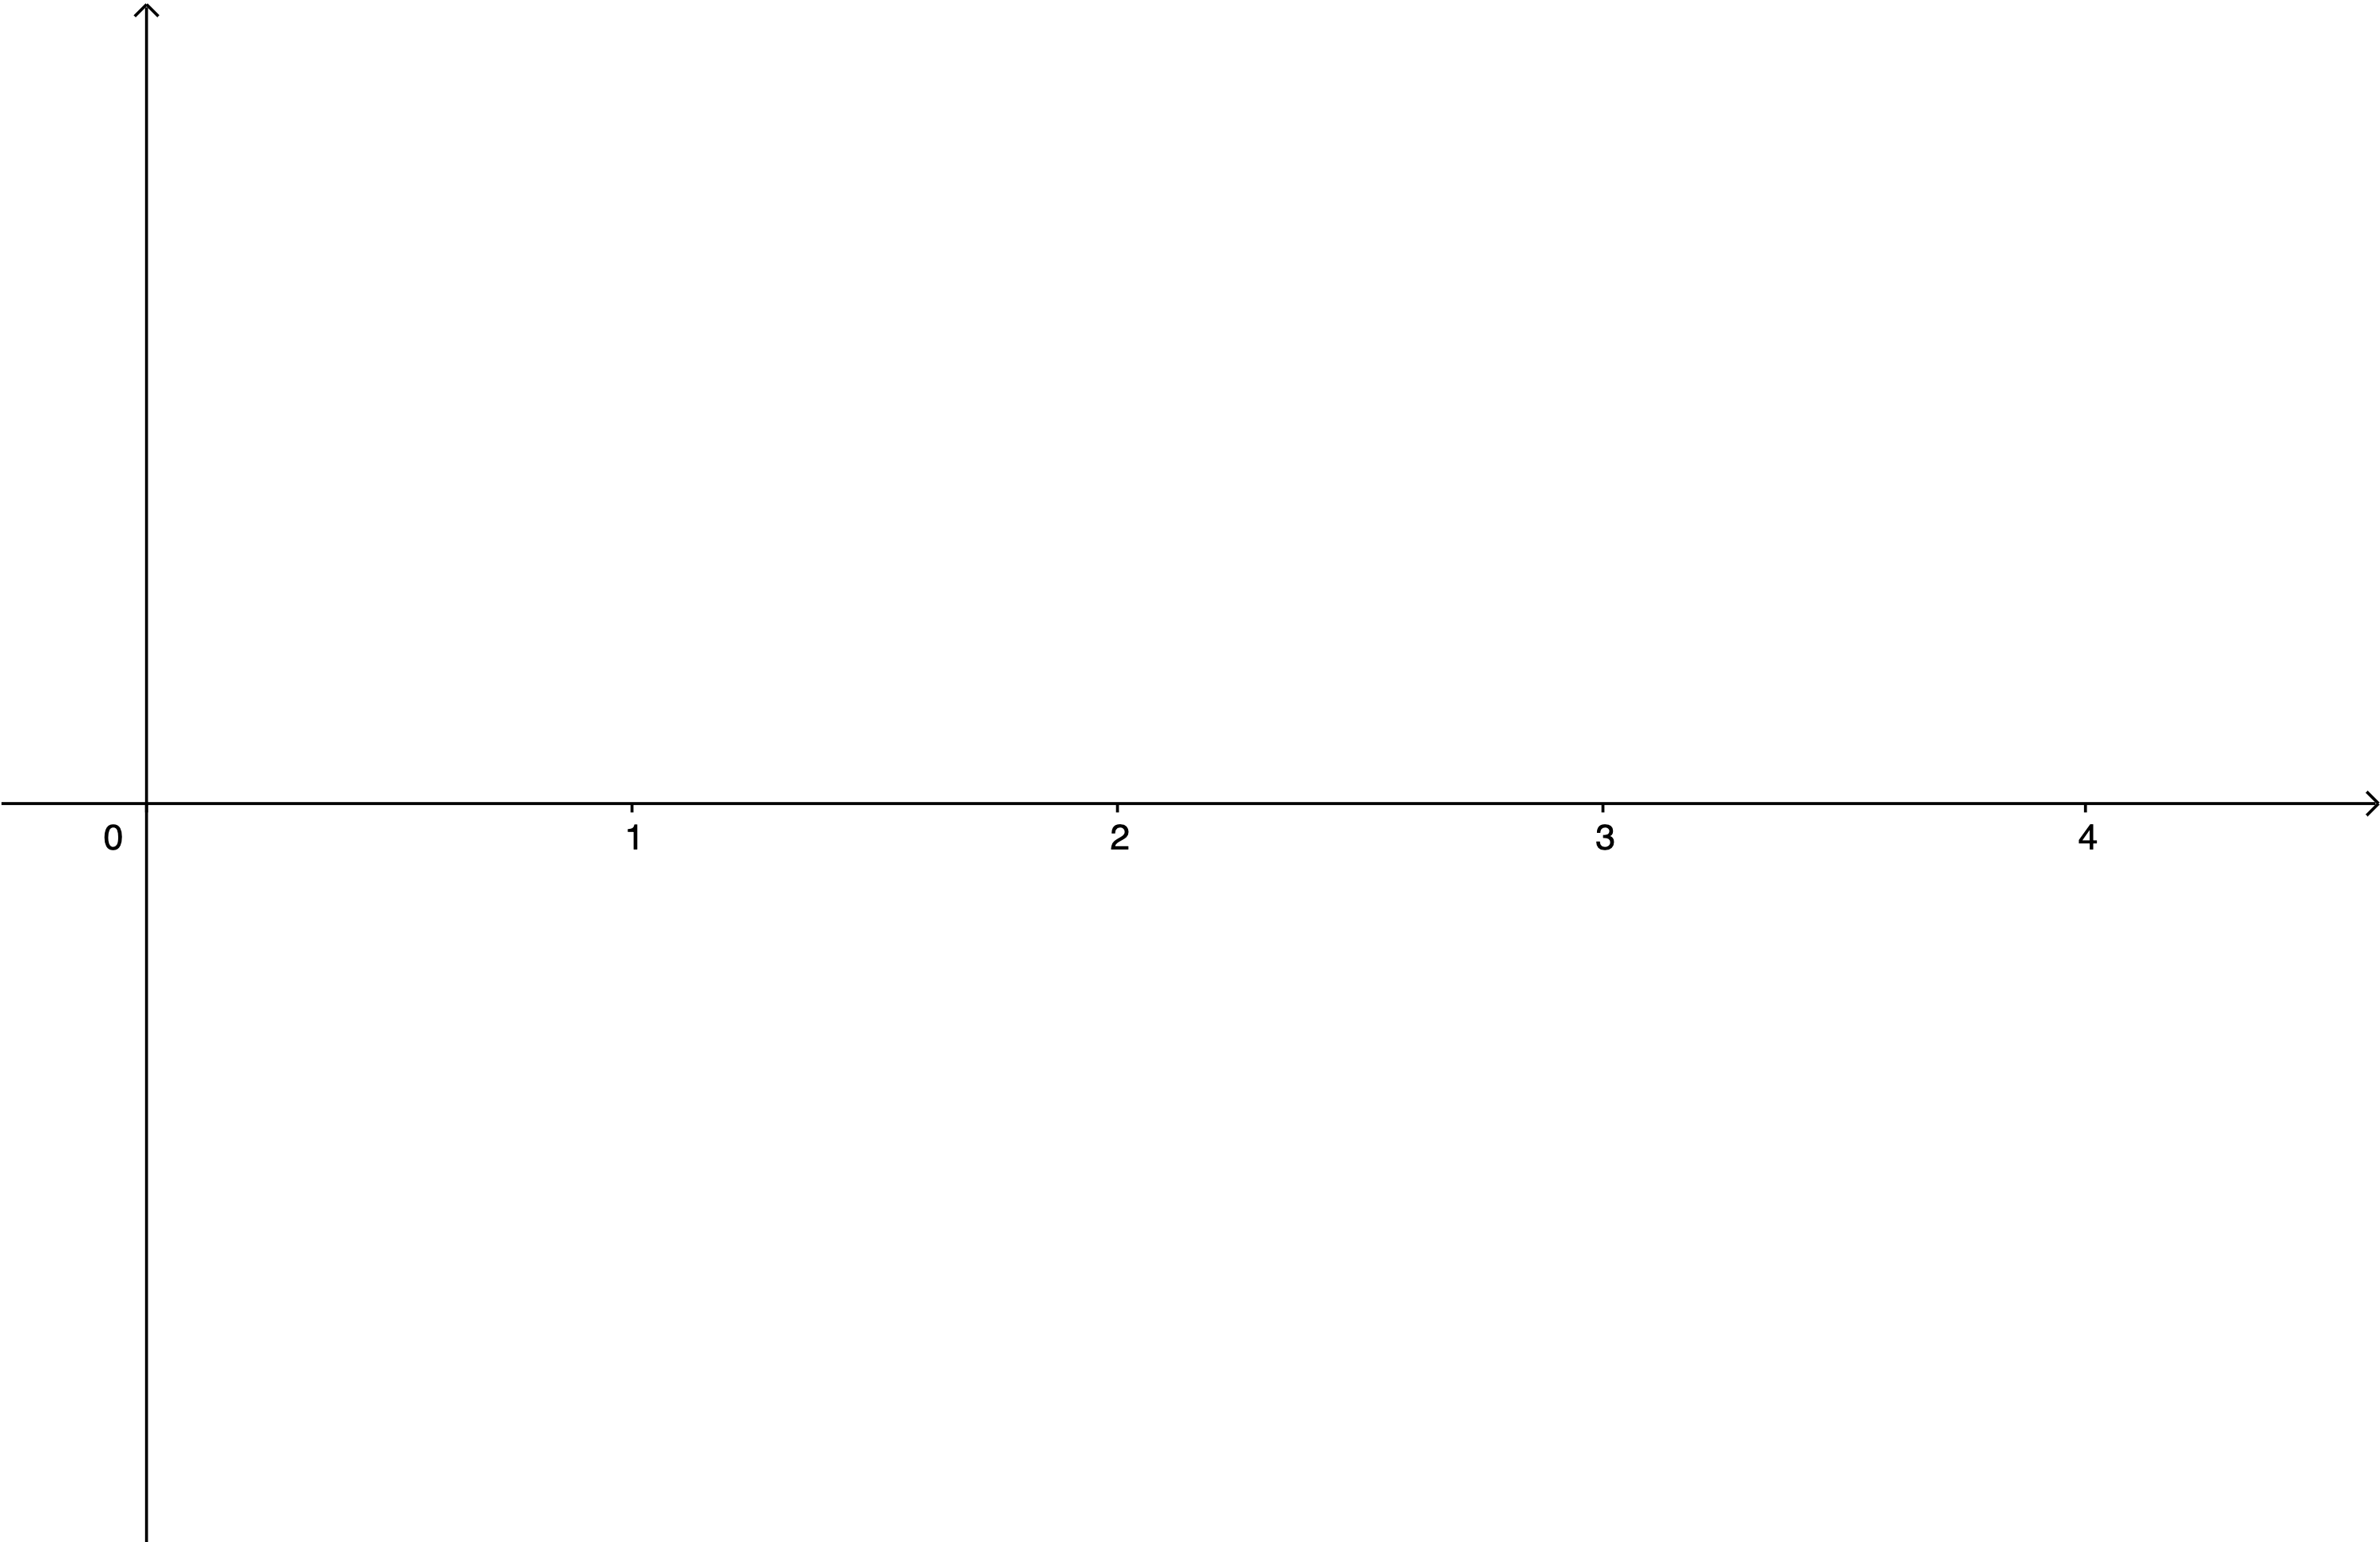
\includegraphics[scale=1.5]{media/KS-hoereAbleitung.png}
		      % \end{center}

		      \begin{center}
			      \begin{tikzpicture}
				      % Achsen
				      \draw[->, thick] (-1,0) -- (9,0) node[right] {$x$};
				      \draw[->, thick] (0,-3) -- (0,3) node[above] {$y$};

				      % Beschriftungen der Achsen
				      \foreach \x in {1,2,3,4} {
						      \draw (2*\x,-0.1) -- (2*\x,0.1);
						      \node[below] at (2*\x,-0.1) {\x };
					      }
			      \end{tikzpicture}
		      \end{center}
		      \pagebreak

		\item Skizzieren Sie nun den Graphen von $h(x)=x^4-4x^3$
		      % \begin{center}
		      %     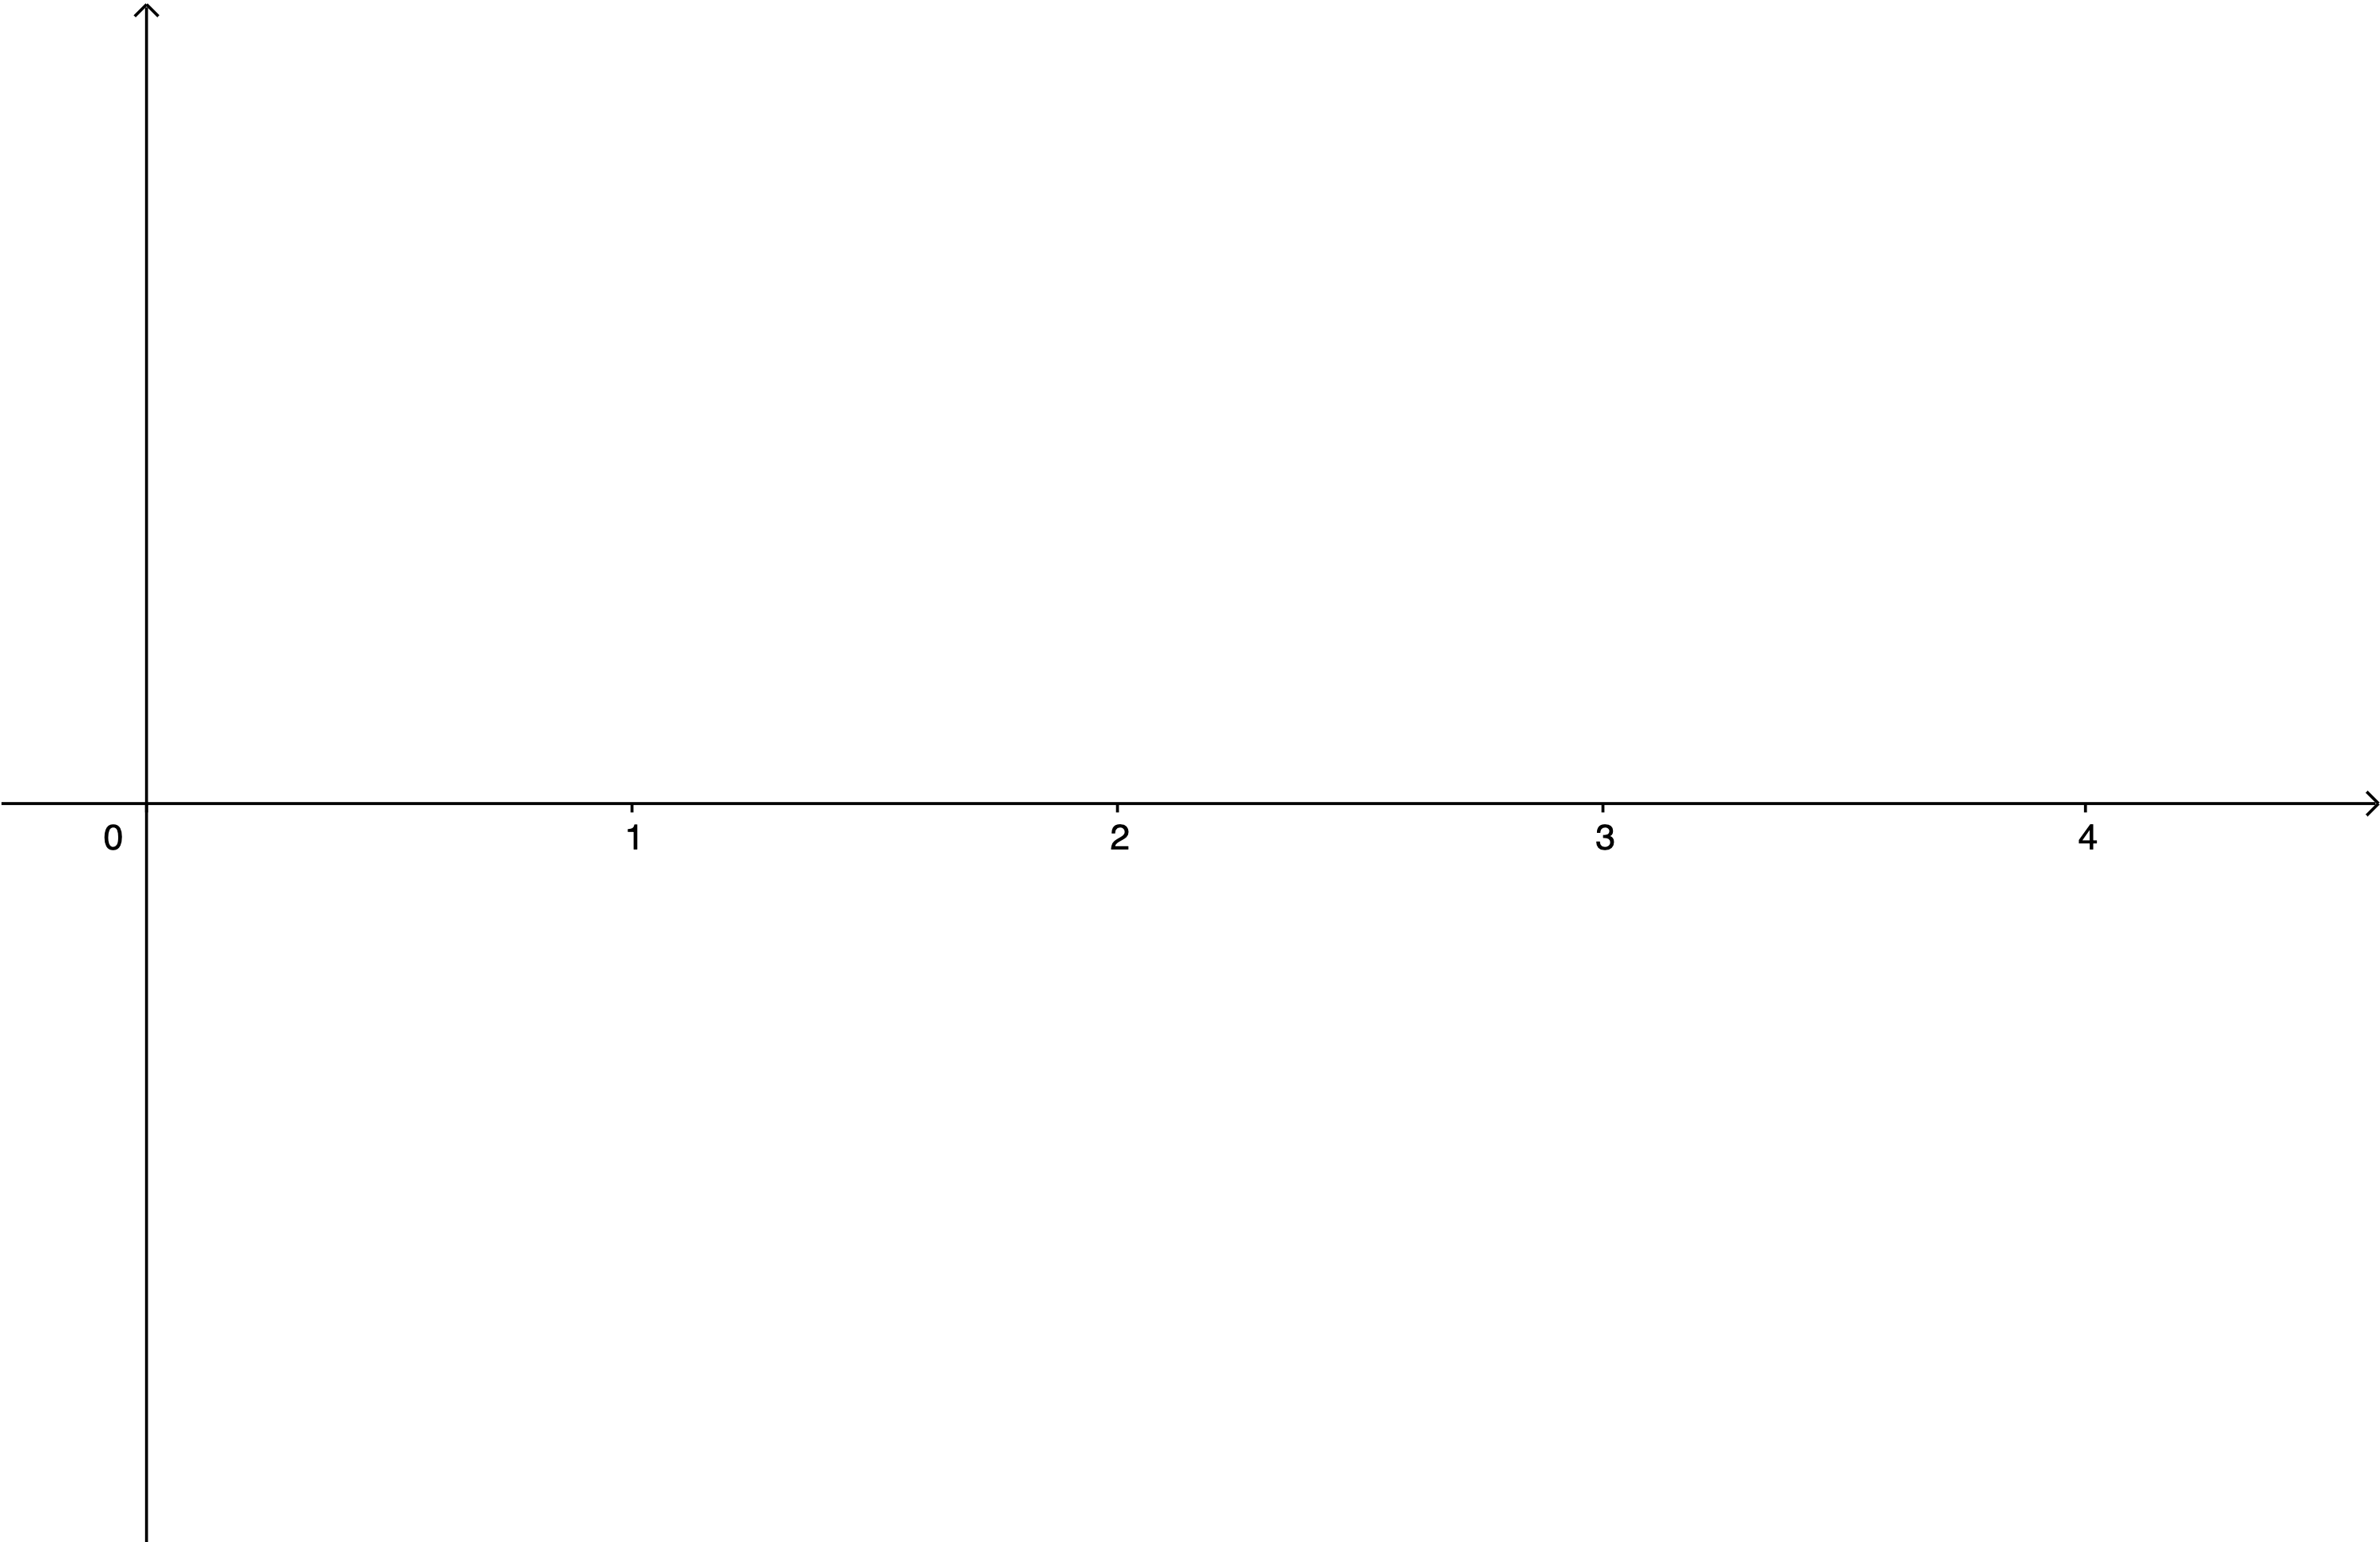
\includegraphics[scale=1.5]{media/KS-hoereAbleitung.png}
		      % \end{center}

		      \begin{center}
			      \begin{tikzpicture}
				      % Achsen
				      \draw[->, thick] (-1,0) -- (9,0) node[right] {$x$};
				      \draw[->, thick] (0,-3) -- (0,3) node[above] {$y$};

				      % Beschriftungen der Achsen
				      \foreach \x in {1,2,3,4} {
						      \draw (2*\x,-0.1) -- (2*\x,0.1);
						      \node[below] at (2*\x,-0.1) {\x };
					      }
			      \end{tikzpicture}
		      \end{center}
		\item Bob möchte den Graphen der Funktion $b(x)=x^4-3x^2$ ungefähr skizzieren. Wie könnte er vorgehen?
	\end{enumerate}
\end{LA}
\clearpage
Einige der Erkenntnisse aus der Einführungsaufgabe – die genauen Rückschlüsse von der Gestalt der Ableitung auf den Graphen der Funktion – werden zu einem späteren Zeitpunkt vertieft werden (Siehe \Cref{speziellePte}). Für den Moment halten wir fest, dass eine differenzierbare Funktion mehrmals abgeleitet werden kann:
\begin{definition}
	{Höhere Ableitung}{}
	Sei $f$ eine differenzierbare Funktion. Da die erste Ableitung $f'$ selbst wieder eine Funktion ist, kann man auch diese in der Regel wieder Ableiten und gelangt so zur zweiten Ableitung der Funktion $f$.

	Schreibweise:
	$$f'' \text{ oder } f^{(2) } \text{ oder } \frac{d^2 f}{dx^2 }$$

	Wenn man von der zweiten Ableitung wieder die Ableitung bildet, erhält man die dritte Ableitung $f'''$, und so weiter.

	Die $n$-te Ableitung ($n\in \N$) der Funktion bezeichnet man allgemein mit
	$$f^{(n)} \text{ oder } \frac{d^n f}{dx^n} $$

\end{definition}

\begin{bsp}
	{}{}
	Gegeben ist die Funktion $f(x)=7x^{10}-5x^3+x$. Die erste Ableitung der Funktion ist
	$$f'(x)=70x^9-15x^2+1$$
	Die zweite Ableitung lautet
	$$f''(x)=630x^8-30x$$
	Die dritte
	$$f'''(x)=5040x^7-30$$
	Die vierte
	$$f^{(4)}(x)=35280x^6$$
	Und so weiter \dots
\end{bsp}
\clearpage
\begin{ueb}
	{}{}
	\begin{enumerate}
		\item Bestimme die 2. Ableitung der gegebenen Funktion.
		      \begin{enumerate}
			      \item \( f(x) = 3x^5 + 4x - 2 \)
			      \item \( f(x) = \frac{1}{12}x^4 - \frac{1}{6}x^3 + \frac{1}{2}x^2 \)
			      \item \( f(x) = (5x - 2)^2 \)
		      \end{enumerate}
		\item
		      \begin{enumerate}
			      \item Bestimme die Ableitungen \( f', f'', f^{(3)}, f^{(4)} \) und \( f^{(5)} \) der angegebenen Funktion.
			            \begin{enumerate}
				            \item \( f(x) = x^3 \)
				            \item \( f(x) = x^4 \)
				            \item \( f(x) = x^5 \)
				            \item \( f(x) = x^6 \)
			            \end{enumerate}
			      \item Wie lautet die 5. Ableitung \( f^{(5)} \) für die Funktion \( f(x) = x^n,\ n \in \mathbb{N} \) mit \( n \geq 5 \)?
			      \item Lässt sich eine Potenzfunktion \( f \) mit \( f(x) = x^n \ (n \in \mathbb{N}) \) beliebig oft ableiten?
		      \end{enumerate}

		\item Gib eine mögliche Funktionsgleichung \( y = f(x) \) mit der gegebenen Eigenschaft an.
		      \begin{enumerate}
			      \item \( y' = x^2 \)
			      \item \( y'' = x^2 \)
			      \item \( y''' = x^2 \)
		      \end{enumerate}

		\item Gegeben ist die Funktion $f(x) = \sin(x)$. Bestimme
		      \begin{enumerate}
			      \item $f'(x), f''(x), f'''(x)$ und $f^{(4)}(x)$.
			      \item $f^{(11)}(x)$ und $f^{(101)}(x)$
		      \end{enumerate}

		\item Sei nun $y=e^{2x}$. Bestimme die Ableitungen $y', y''$ und $y^{(10)}$

		\item Gegeben ist $g(x) = x\cdot e^x$. Bestimme $g'(x)$ und $g''(x)$. Wie lautet wohl eine Formel für die $n$-te Ableitung $g^{(n)}(x)$?
	\end{enumerate}

\end{ueb}

\clearpage
\emph{Lösungen:}
\begin{enumerate}
	\item
	      \begin{enumerate}
		      \item \( f''(x) = 60x^3 \)
		      \item \( f''(x) = x^2 -x + 1 \)
		      \item \( f''(x) = 50 \)
	      \end{enumerate}

	\item
	      \begin{enumerate}
		      \item
		            \begin{enumerate}
			            \item
			                  \begin{align*}
				                  f'(x)      & = 3x^2 \\
				                  f''(x)     & = 6x   \\
				                  f^{(3)}(x) & = 6    \\
				                  f^{(4)}(x) & = 0    \\
				                  f^{(5)}(x) & = 0
			                  \end{align*}
			            \item
			                  \begin{align*}
				                  f'(x)      & = 4x^3  \\
				                  f''(x)     & = 12x^2 \\
				                  f^{(3)}(x) & = 24x   \\
				                  f^{(4)}(x) & = 24    \\
				                  f^{(5)}(x) & = 0
			                  \end{align*}
			            \item
			                  \begin{align*}
				                  f'(x)      & = 5x^4  \\
				                  f''(x)     & = 20x^3 \\
				                  f^{(3)}(x) & = 60x^2 \\
				                  f^{(4)}(x) & = 120x  \\
				                  f^{(5)}(x) & = 120
			                  \end{align*}
			            \item
			                  \begin{align*}
				                  f'(x)      & = 6x^5   \\
				                  f''(x)     & = 30x^4  \\
				                  f^{(3)}(x) & = 120x^3 \\
				                  f^{(4)}(x) & = 360x^2 \\
				                  f^{(5)}(x) & = 720x
			                  \end{align*}
		            \end{enumerate}
		      \item \( f^{(5)}(x) = n(n-1)(n-2)(n-3)(n-4)x^{n-5} \)
		      \item Ja.
	      \end{enumerate}

	\item  Jede Teilaufgabe hat unendlich viele Lösungen. Die einfachsten Lösungen sind:
	      \begin{enumerate}
		      \item \( f(x) = \frac{1}{3}x^3\)
		      \item \( f(x) = \frac{1}{12}x^4  \)
		      \item \( f(x) = \frac{1}{60}x^5  \)
	      \end{enumerate}

	\item
	      \begin{enumerate}
		      \item
		            \begin{align*}
			            f'(x)      & = \cos(x)  \\
			            f''(x)     & = -\sin(x) \\
			            f^{(3)}(x) & = -\cos(x) \\
			            f^{(4)}(x) & = \sin(x)
		            \end{align*}
		      \item
		            \begin{align*}
			            f^{(11)}(x)  & = -\cos(x) \\
			            f^{(101)}(x) & = \cos(x)
		            \end{align*}
	      \end{enumerate}

	\item
	      \begin{align*}
		      y'       & = 2e^{2x}                   \\
		      y''      & = 4e^{2x}                   \\
		      y^{(10)} & = 2^{10}e^{2x} = 1024e^{2x}
	      \end{align*}

	\item
	      \begin{align*}
		      g'(x)      & =(x+1) e^x  \\
		      g''(x)     & = (x+2) e^x \\
		      g^{(n)}(x) & = (x+n)e^x
	      \end{align*}
\end{enumerate}



















% Ausgelassen in 2024 und 2025
% \clearpage
% \subsubsection{Erste Bekanntschaft mit Differentialgleichungen}
% Die Theorie zu diesem Kapitel wird in der Klasse erarbeitet. 

% \begin{definition}{Differentialgleichung}{}
%     Eine \emph{Differentialgleichung (DGL)} ist eine Gleichung, in der eine unbekannte Funktion $y=y(x)$ und ihre Ableitungen $y', y'', y^{(3)}, \ldots $ vorkommen.
% \end{definition}
% Bemerkungen:
% \begin{itemize}
%     \item Im Unterschied zu gewöhnlichen Gleichungen sind bei DGL unbekannte \emph{Funktionen} gesucht!
%     \item DGL haben in der Regel unendlich viele Lösungen.
%     \item Das Bestimmen einer Lösung ist häufig ein schwieriges Unterfangen (siehe AM).
% \end{itemize}

% \begin{ueb}{}{}
%     Übungen im Analysis-Buch auf Seite 66.


%     Dazu die folgende \emph{Challenge}:

%     Der Graph einer Funktion $y=f(x), \, (x>0)$ soll durch den Punkt $(1|2)$ verlaufen und die Eigenschaft haben, dass die Tangente im Kurvenpunkt $(x | f(x))$ die $x$-Achse im Punkt $(2x|0)$ schneidet. Geben Sie die Funktion $f(x)$ an.

%     \begin{center}
%         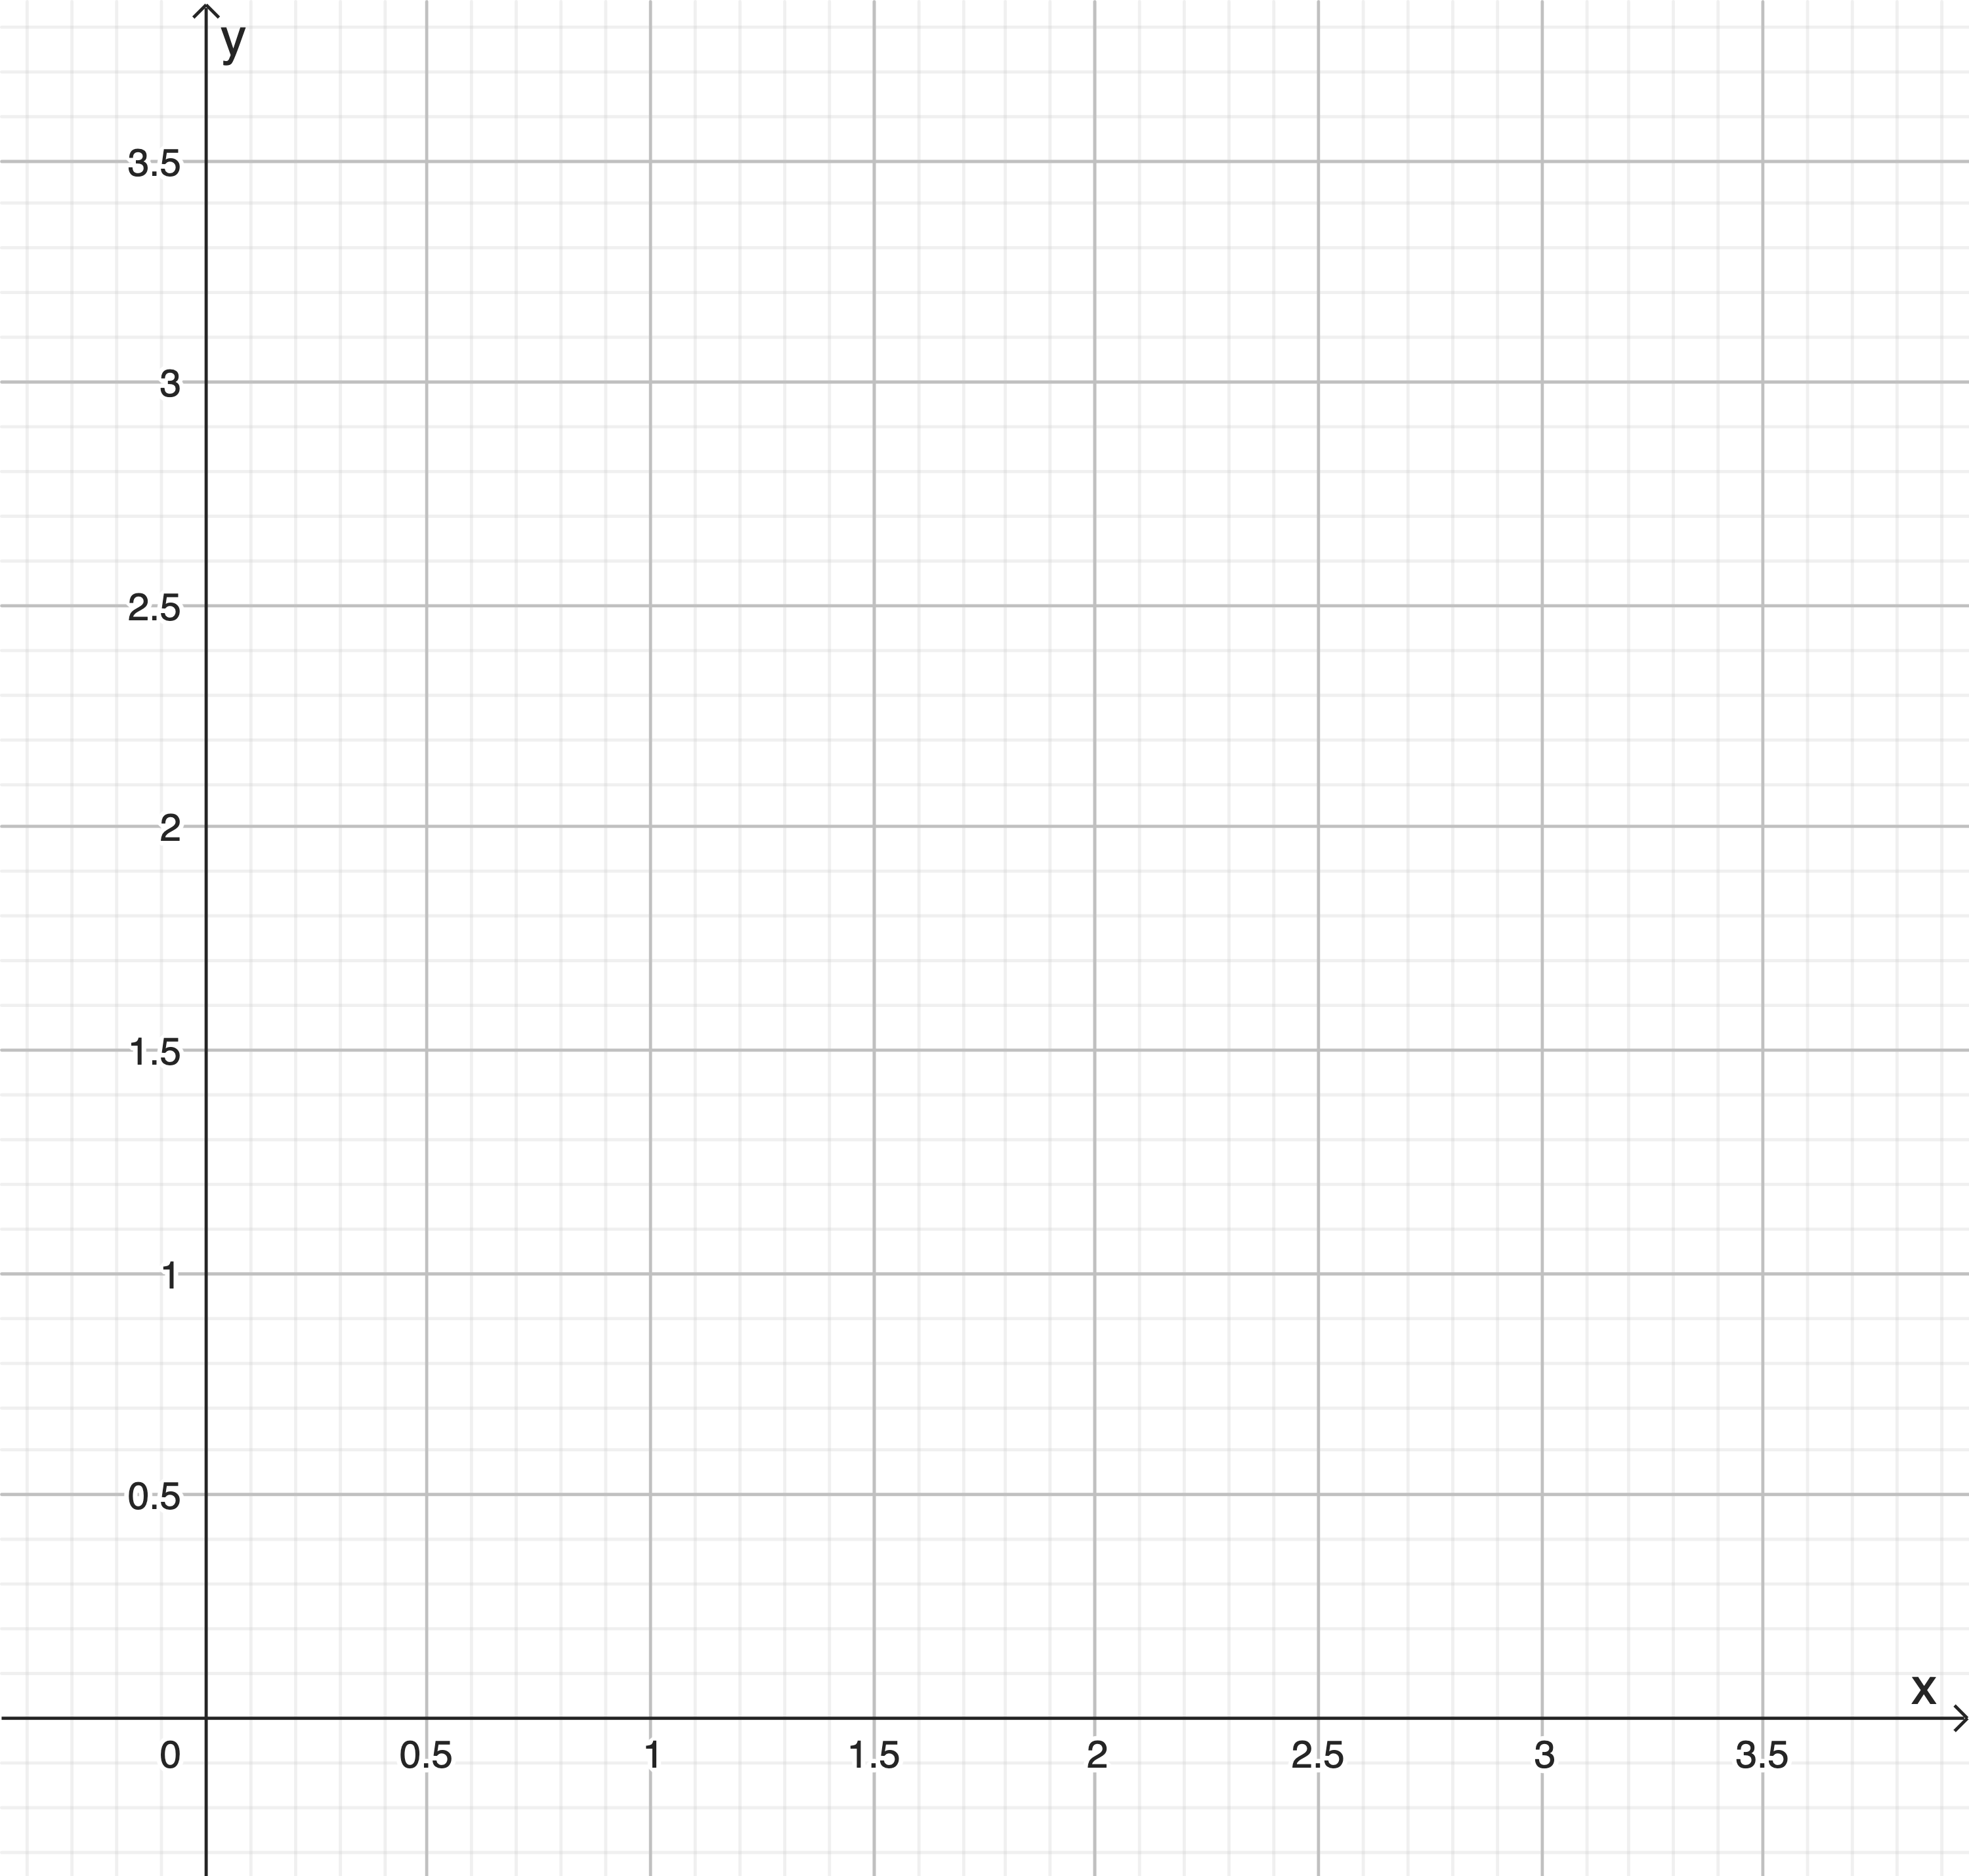
\includegraphics[scale = 2.5]{media/DGL-Knobel-To.png}
%     \end{center}
% \end{ueb}





\clearpage
\subsection{Kurven, die sich berühren, Normale und Schnittwinkel}
\label{Winkel}
\subsubsection{Berühren}

% \begin{LA}
%     {Einführungsaufgaben}{}
%     \begin{enumerate}
%         \item Zeichnen Sie mit \href{https://www.geogebra.org}{Geogebra} in einem Koordinatensystem den Graphen der Funktion $f(x) = x^2-2x$ und die Gerade $t: \, y= 4x-9$. Fügen Sie die Grafik in dieses Dokument ein.
%         \item Weisen Sie nach, dass die Gerade $t$ eine Tangente an den Graphen von $f$ ist, indem Sie rechnerisch überprüfen, dass beide an der Stelle $x=3$ durch denselben Punkt verlaufen ($f(3)=t(3)$) und die gleiche Steigung haben. ($f'(3)=t'(3)$).
%         \item Berechnen Sie die Gleichung der Tangente $t_2$, welche den Graphen von $f$ an der Stelle $x=2$ berührt. Nutzen Sie dazu den Ansatz $t_2 : \, y=ax+b$ und ermitteln Sie $a$ und $b$ mit geeigneten Gleichungen.
%         \item Zeichnen Sie auch die Gerade $t_2$ mit Geogebra und überprüfen Sie so da Resultat.
%         \item Bestimmen Sie rechnerisch die Gleichung der Tangente, welche den Graphen von $g(x)= \frac{x}{x-1}$ an der Stelle $x=-1$ berührt und überprüfen Sie das Ergebnis mit Geogebra.
%         \item Geben Sie ein \glqq Rezept\grqq{} an, wie man allgemein die Gleichung der Tangente $t$ bestimmen kann, welche den Graphen einer Funktion $f$ an einer vorgegebenen Stelle $x_0$ bestimmen kann.
%     \end{enumerate} 
% \end{LA}
% \clearpage

Die Ableitung $f'(x_0)$ an einer bestimmten Stelle $x_0$ ist geometrisch gesehen die Steigung der Tangente an den Graphen der Funktion $f$. Damit haben wir schon mehrmals die Gleichung der Tangente an einen Funktionsgraphen ermittelt.
\begin{bsp}
    {Warm up}{}
    Wir betrachten als Beispiel den Graphen der Funktion $f(x)=x\cdot \ln(x) $
    \begin{center}
        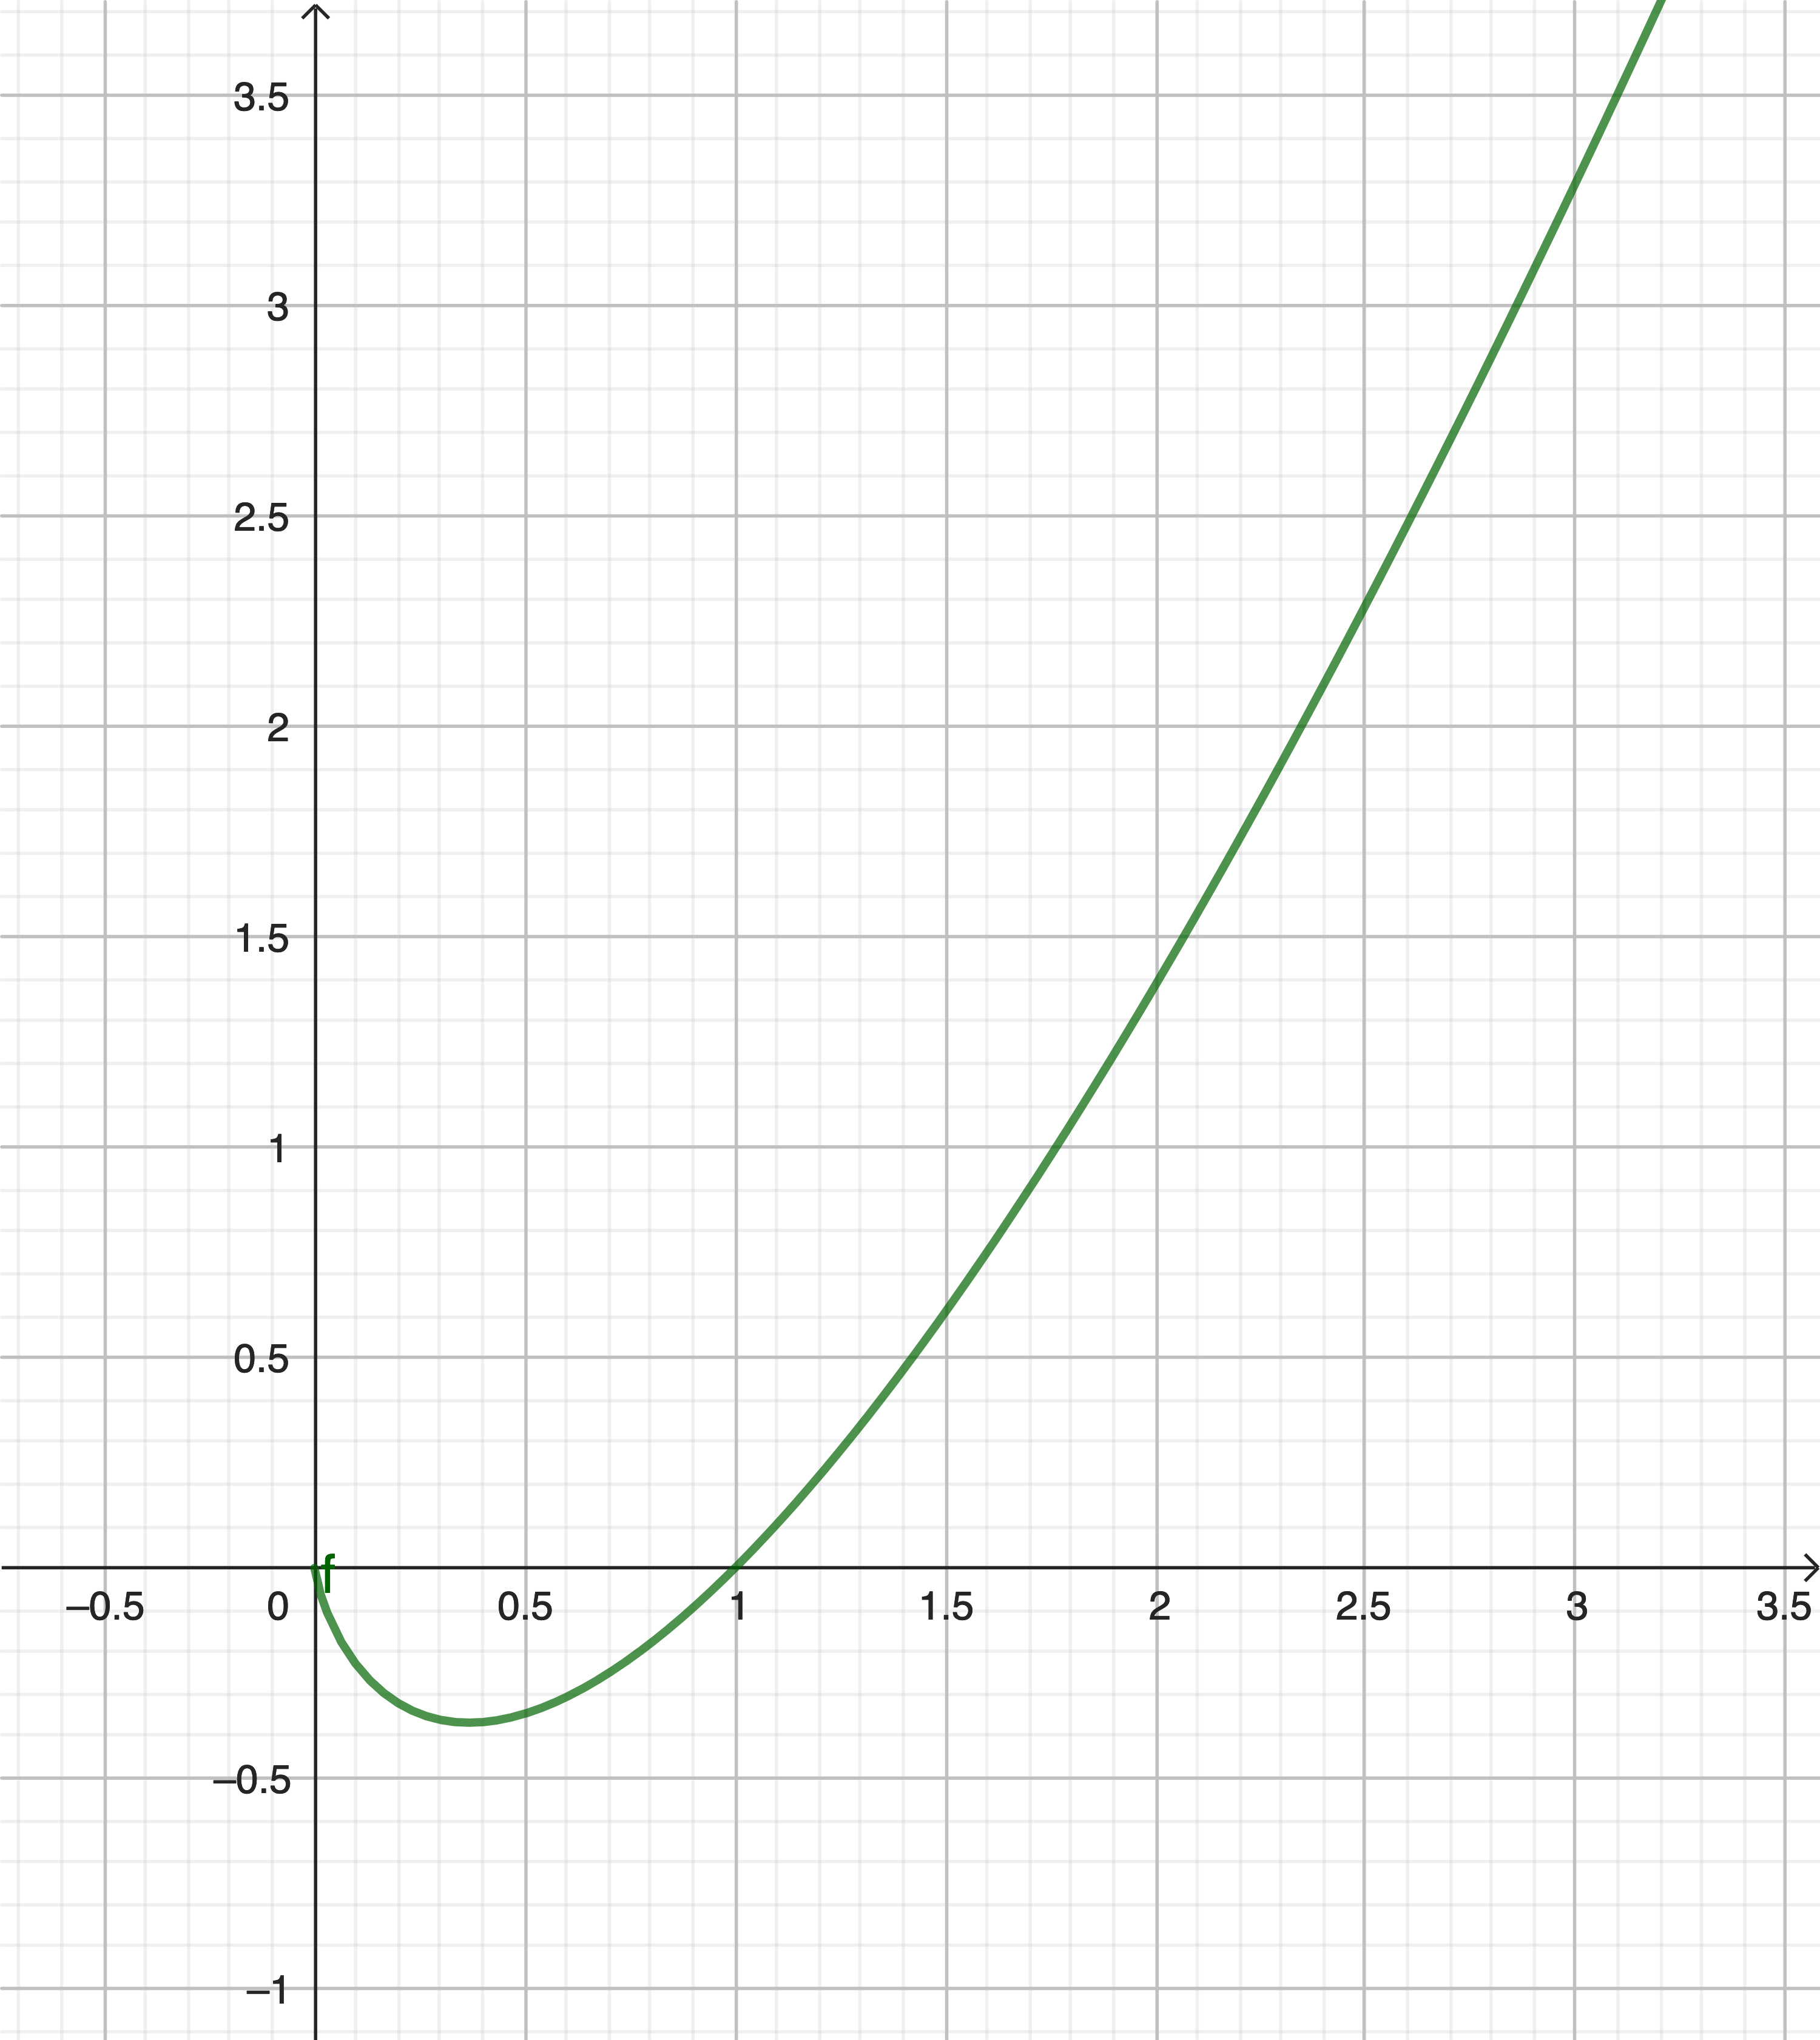
\includegraphics[scale=1]{media/xlnx.png}
    \end{center}
    Gesucht ist die Gleichung der Tangente an den Graphen an der Stelle $x=e$.
    \vspace*{10cm}
    % Ansatz: $t: \, y=ax+b$

    % An der Berührungsstelle haben Tangente und Kurve die gleiche Steigung: $a = f'(e)$ wobei $f'(x)=1\cdot \ln(x) + x\cdot \frac{1}{x}= \ln(x)+1$. Also
    % $$a=f'(e)=\ln(e)+1=2 \Longrightarrow t: \, y= 2x+b$$
    
\end{bsp}
\clearpage
\begin{satz}{Tangente an einen Funktionsgraphen}{}
    Eine Gerade $t: \, y = ax+b$ ist genau dann die Tangente an den Graphen der Funktion $f$ an der Stelle $x_0$, wenn gilt
    $$t'(x_0)=f'(x_0) \qquad \text{und} \qquad t(x_0)=f(x_0)$$

    Man sagt dann, dass die Gerade $t$ den Graphen von $f$ an der Stelle $x_0$ \emph{berührt}.
\end{satz}
Im Unterschied zu Kreistangenten oder auch Tangenten an Parabeln können Tangenten an allgemeine Funktionsgraphen auch mehrere gemeinsame Punkte mit dem dem Graphen haben. Die Gerade im Bild unten \emph{berührt} den Funktionsgraphen im Punkt $B$ und \emph{schneidet} ihn ausserdem an der Stelle $x=-1.5$
\begin{center}
    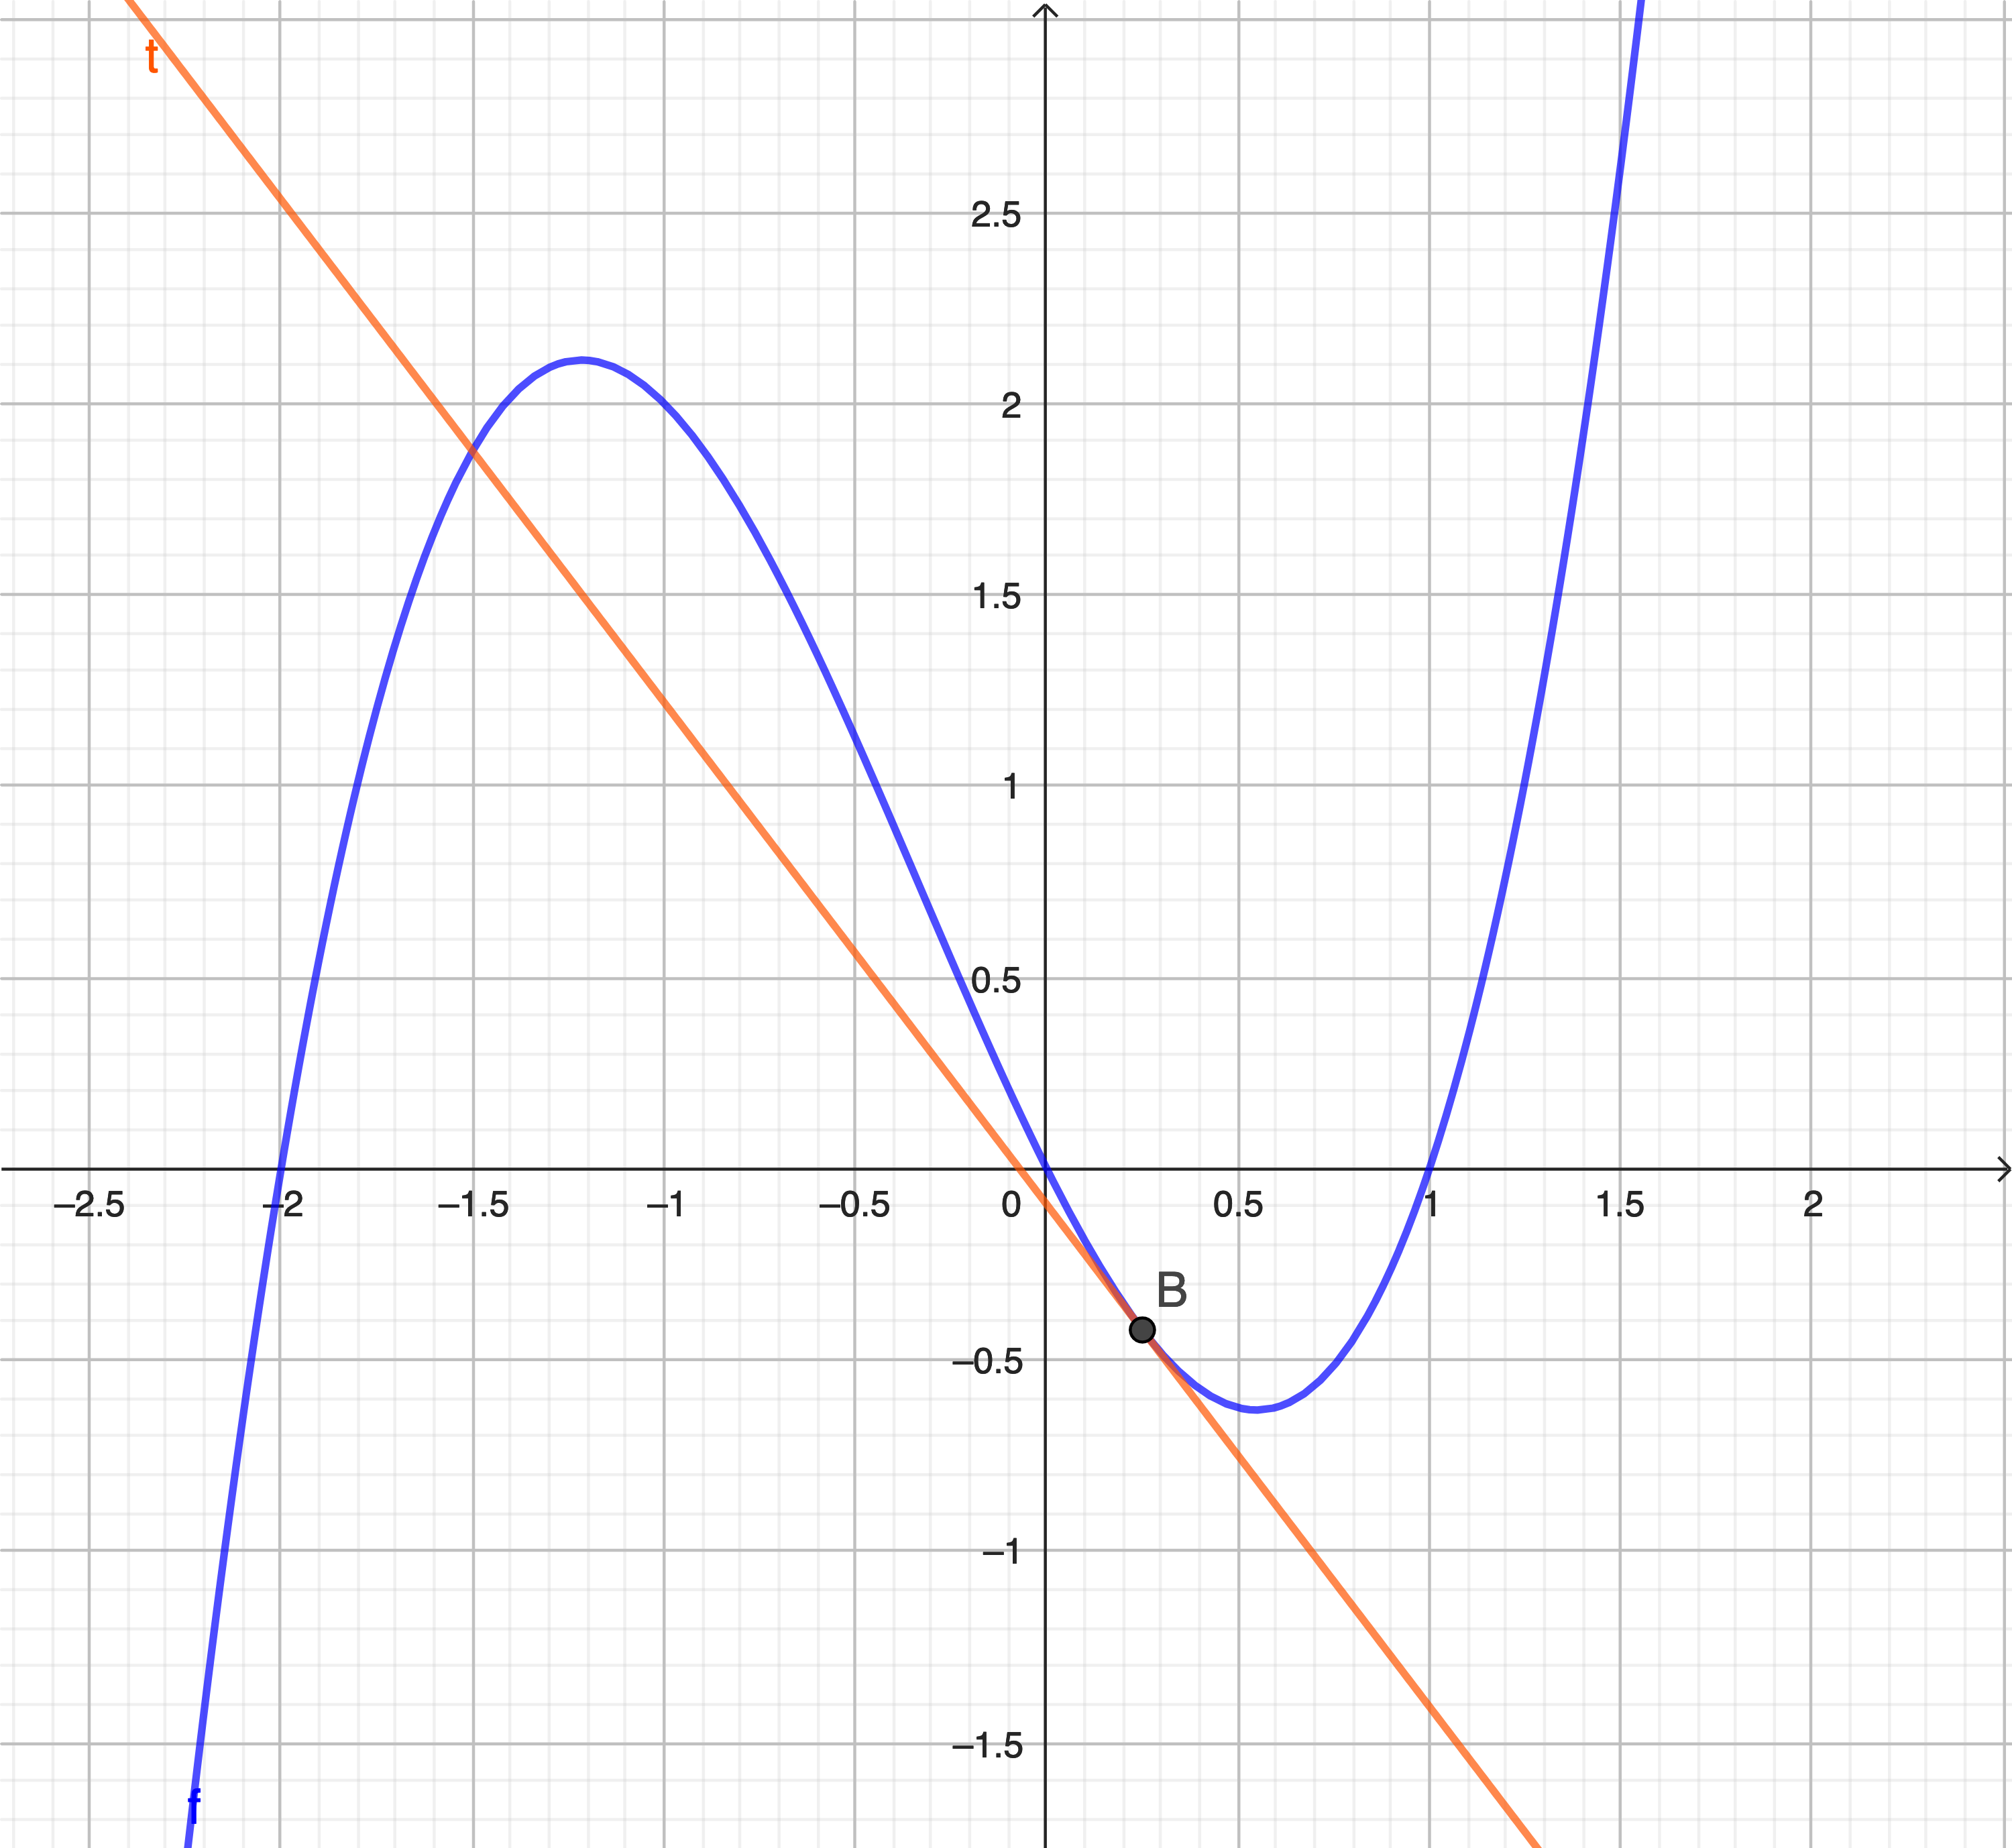
\includegraphics[scale = 1.3]{media/tangenteDef.png}
\end{center}
 
Nicht nur Geraden und Graphen können sich berühren, auch Graphen und andere Graphen:
\begin{definition}{Graphen, die sich berühren}{}
    Wenn für zwei Funktionen $f$ und $g$ gilt
    $$f'(x_0)=g'(x_0) \qquad \text{und} \qquad f(x_0)=g(x_0)$$
    Dann sagt man, dass sich die beiden Funktionsgraphen  an der Stelle $x_0$ \emph{berühren}.
\end{definition}

Bemerkung: Wenn sich zwei Graphen berühren, haben sie im Berührungspunkt eine gemeinsame Tangente.

\begin{center}
    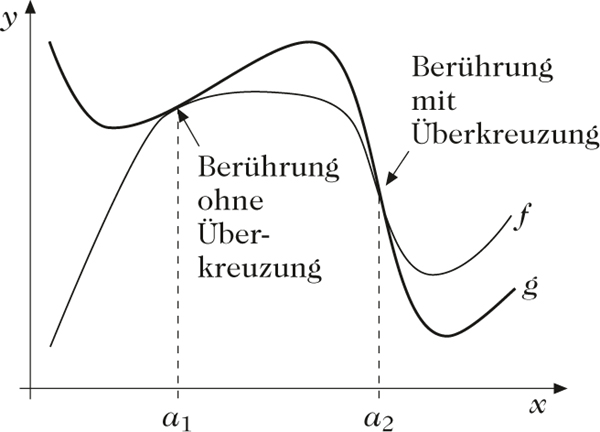
\includegraphics[scale=0.2]{media/Beruhrung-zweier-Funktionen-I11.jpg}
\end{center}


\clearpage
\begin{ueb}{}{}
    \begin{enumerate}
        \item Zeigen Sie, dass sich die Graphen der Funktionen $f(x) = x^2-3$ und $g(x) = x^3-x-2$ an der Stelle $x=1$ berühren.
        \item Zeigen Sie, dass sich die Graphen der Funktionen $f(x) = e^{x-2}$ und $g(x) = \left(\frac{x}{2}\right)^2$ an der Stelle $x=2$ berühren. \\
        Berechnen Sie anschliessend die Nullstelle der gemeinsamen Tangente.
        \item Gegeben sind die Funktionen $f(x) = \sin(x)$ und $g(x) = c- \cos(x)$. Bestimmen Sie den Wert von $c\in \R$, sodass sich die beiden Graphen im Bereich $x\in [0, 2\pi]$ berühren.\\
        Tipp: Wenn die Gleichung für den Vergleich der Steigungen schwierig zu lösen ist, versuchen Sie beide Seiten durch $\cos(x)$ zu teilen.
    \end{enumerate}
\end{ueb}


\emph{Lösungen:}
\begin{enumerate}
    \item \dots
    \item Nullstelle der gemeinsamen Tangente: $x=1$
    \item $x= \sqrt{2}$
\end{enumerate}

























\clearpage
\subsubsection{Schnittwinkel}
\begin{LA}
    {Einführungsaufgabe zu Schnittwinkel und Senkrechtstehen}{}
    \begin{enumerate}
        \item Winkel zwischen Kurven: \newline
        Beim Wiedereintritt einer bemannten Raumkapsel muss der Winkel, in dem die Raumkapsel in die Atmosphäre eindringt, in einem ganz bestimmten Bereich liegen. Wenn die Raumkapsel zu flach auf die Atmosphäre eintrifft, prallt sie ab. Wenn der Winkel zu steil ist, verglüht sie.
        Wie misst man aber den Winkel zwischen zwei \glqq krummen\grqq{} Linien? Messen Sie den ungefähren Aufprallwinkel in der Skizze unten. 
        \begin{center}
            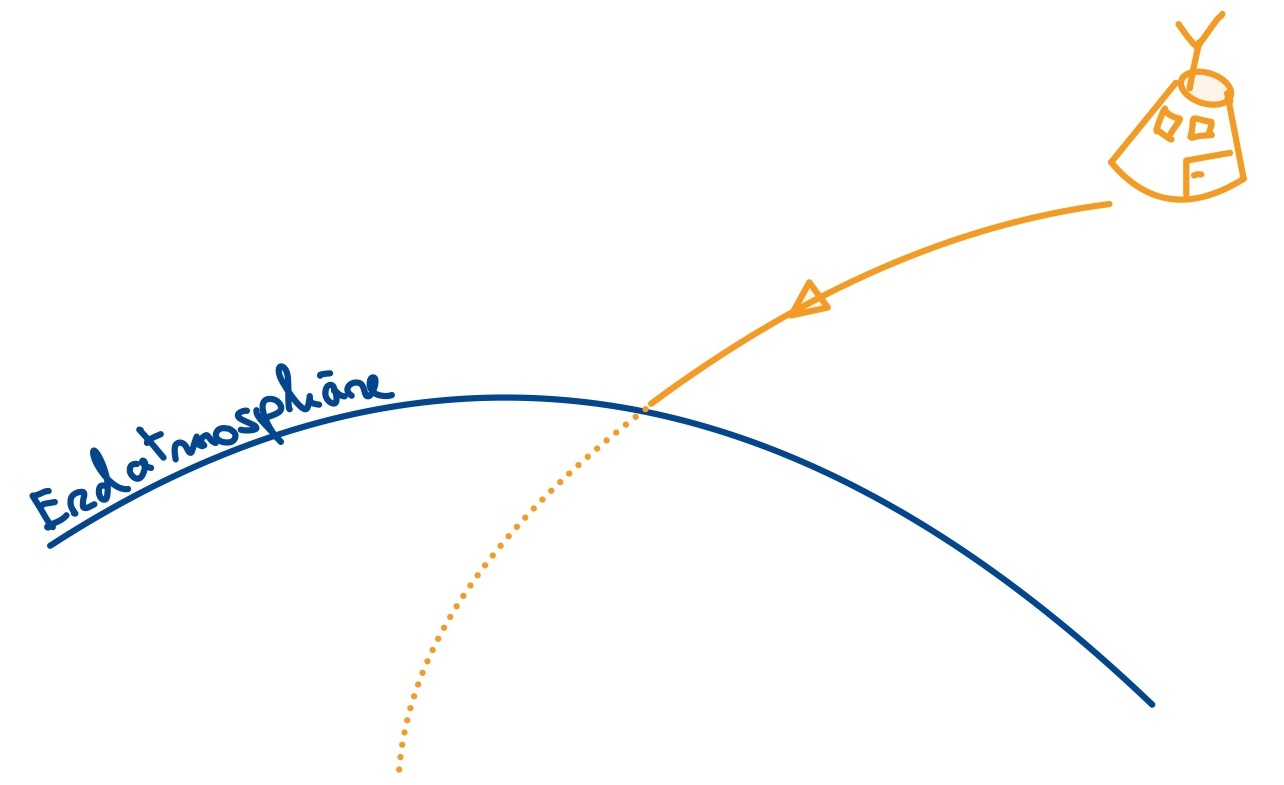
\includegraphics[width = 0.6\textwidth]{media/IntroWinkel.jpg}
        \end{center}
        \item Senkrechte Geraden: \newline
        Im Bild ist der Graph der Geraden $g: \,  y=2x$ dargestellt. Zeichnen Sie die Senkrechte zur Geraden durch den Punkt $A$. Welche Steigung hat sie? Wie erkennt man an der Steigung, ob zwei Geraden senkrecht stehen?
        \begin{center}
            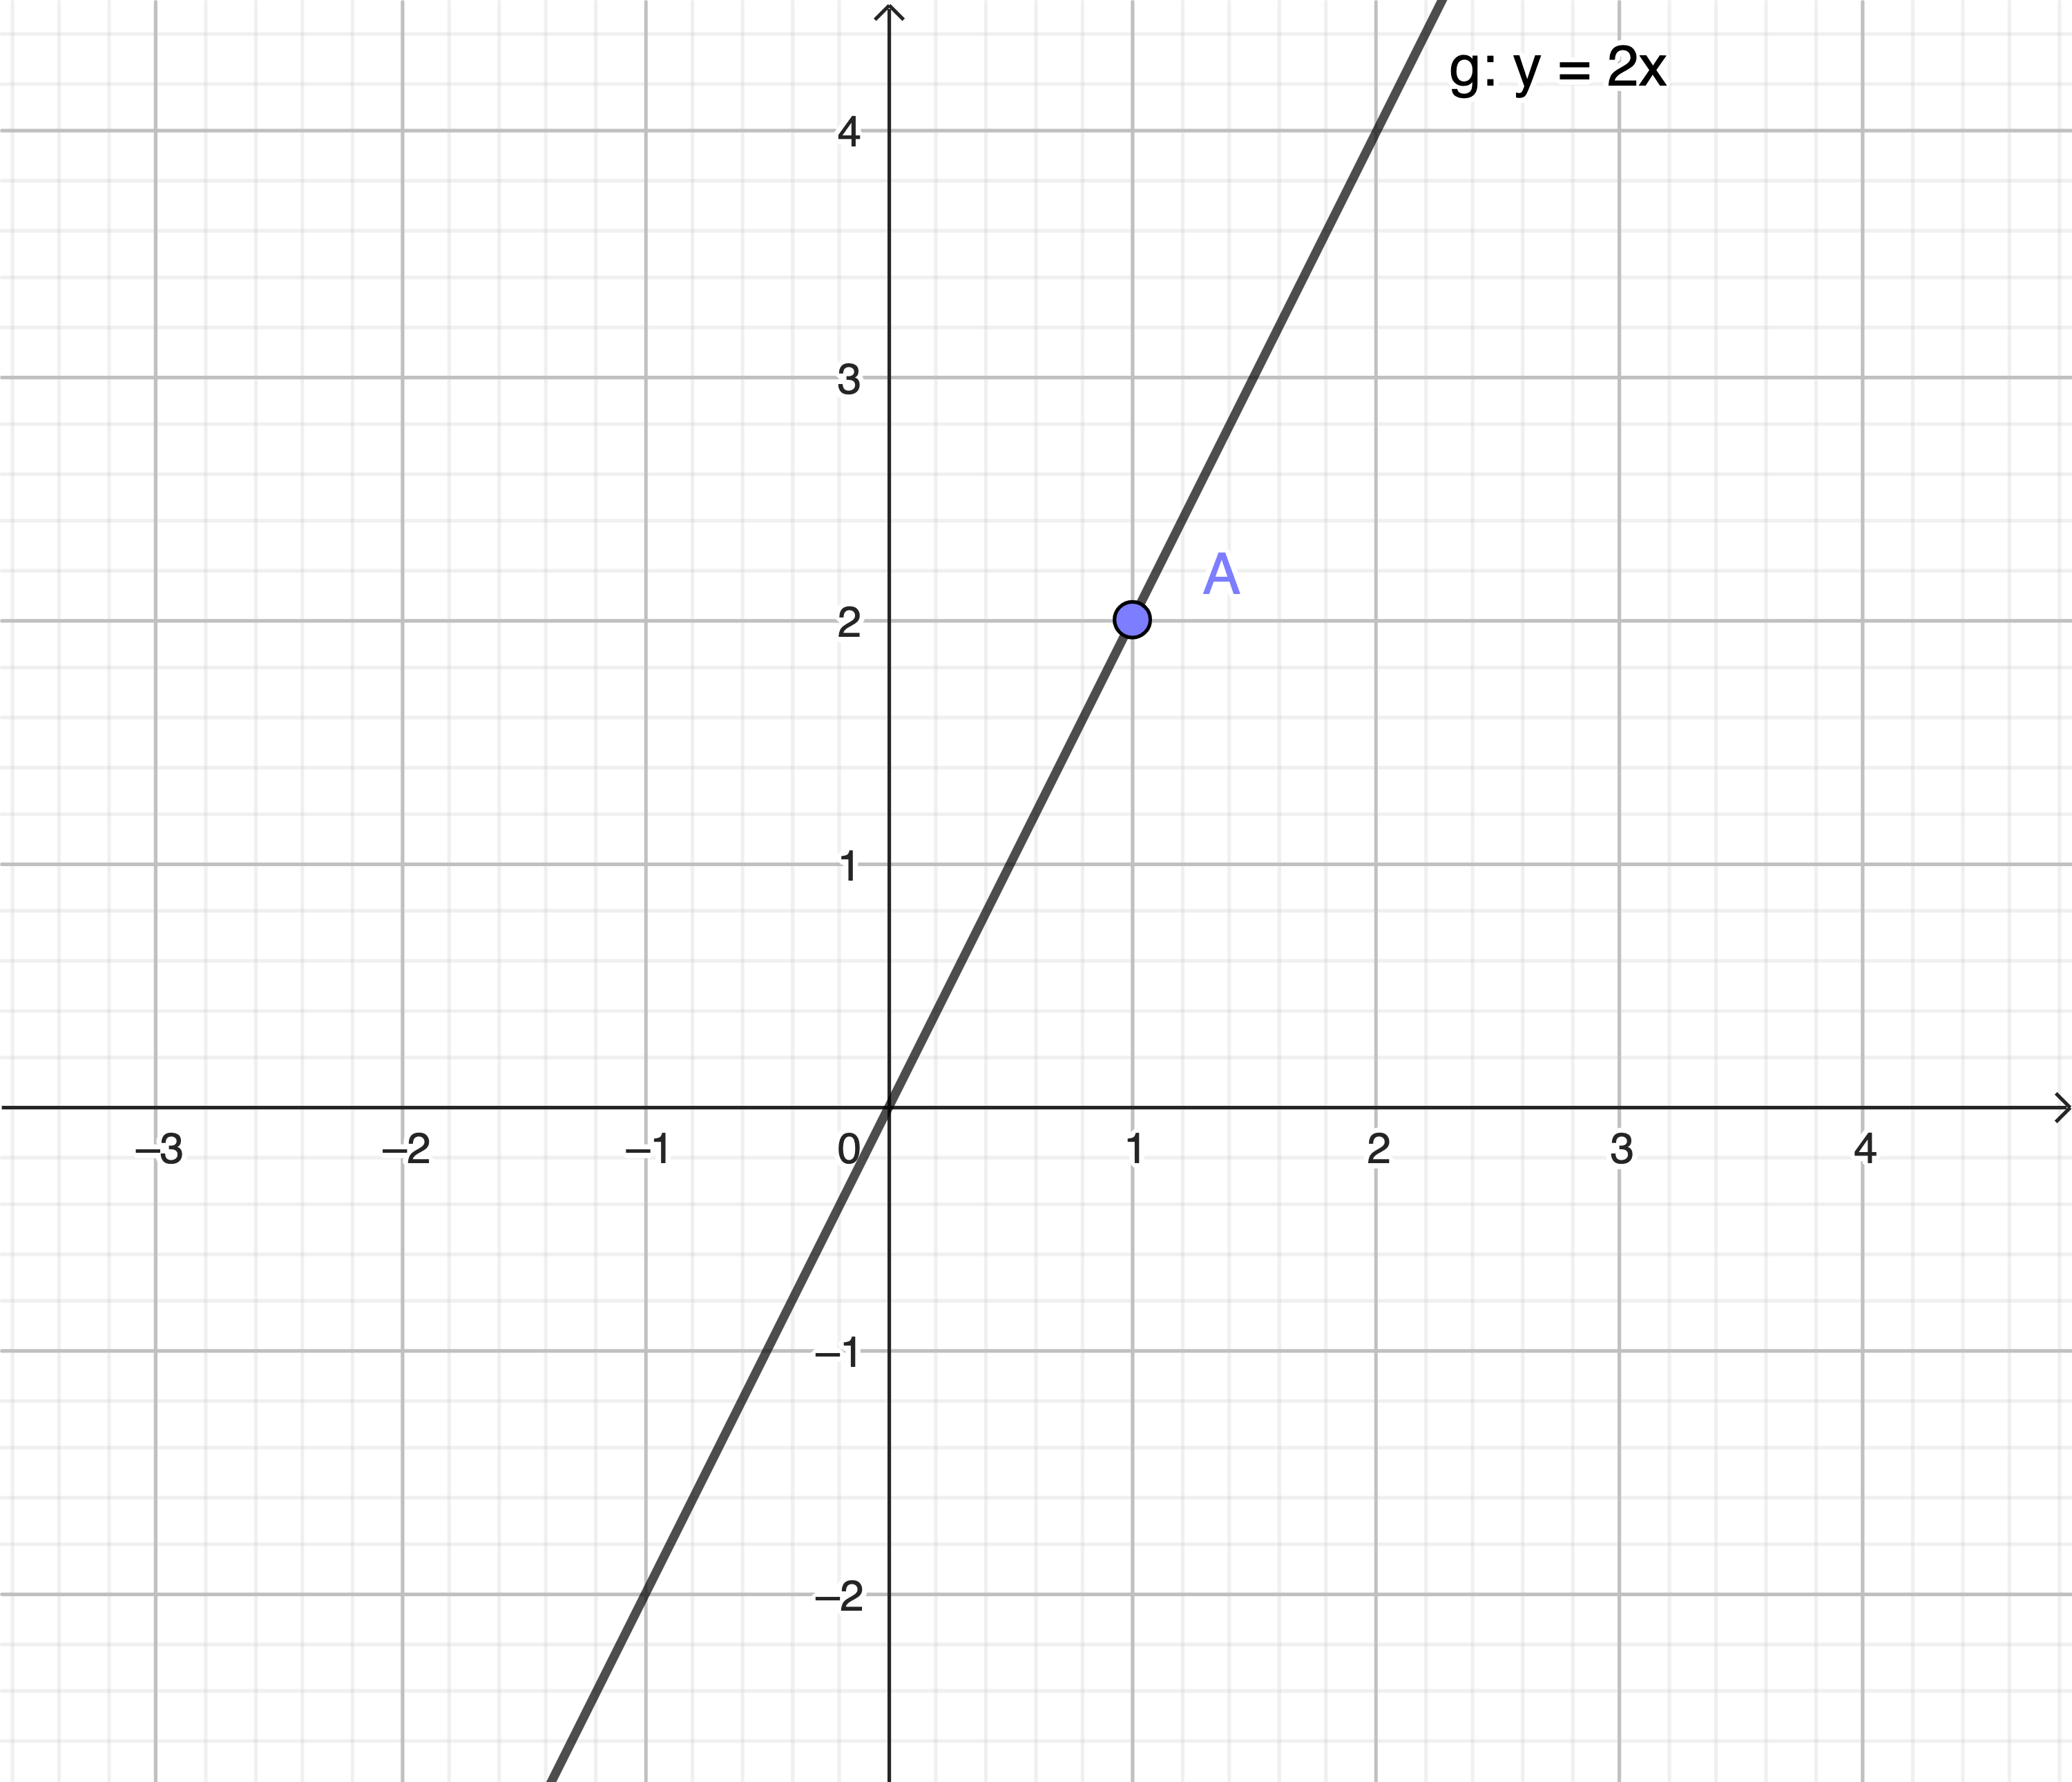
\includegraphics[width = 0.6\textwidth]{media/senkrechteGeraden.png}
        \end{center}
        \newpage
        \item Winkelberechnung: 
        \begin{enumerate}
            \item Zeichnen Sie in den Graphen der Geraden $y=2x$ oben das Steigungsdreieck mit den Ecken $(0|0), (1|0)$ und $A$.
            \item Berechnen Sie den Winkel $\alpha$ zwischen der Geraden $g$ und der $x$-Achse (Verwenden Sie dazu den Tangens!).
            \item Zeichnen Sie die Gerade $h$ durch den Ursprung mit der Steigung $a=\frac{1}{3}$. Welchen Winkel $\beta$ bildet sie mit der $x$-Achse?
            \item Welchen Winkel schliessen die beiden Geraden $g$ und $h$ ein?
        \end{enumerate}
        \item Formeln:
        \begin{enumerate}
            \item Geben Sie eine Formel an, mit der man den Winkel zwischen den beiden Geraden $g:\,   y=a_1 x+b_1$ und $h:\,  y=a_2 x+b_2$ berechnen kann.
            \item  Stimmt die Formel auch, wenn eine oder beide Steigungen negativ sind? Wieso?
        \end{enumerate} 
    \end{enumerate}
\end{LA}
\clearpage
Im Folgenden Abschnitt wird das Verfahren zur Berechnung des Schnittwinkels zwischen zwei Funktionsgraphen erklärt. Bevor damit begonnen wird, muss allerdings zuerst erklärt werden, was unter dem Winkel zwischen zwei \glqq krummen Linien\grqq{} gemeint ist:
\begin{definition}
    {Schnittwinkel}{}
    Der Schnittwinkel von zwei Kurven ist der Winkel zwischen den Kurventangenten im Schnittpunkt:
    \begin{center}
        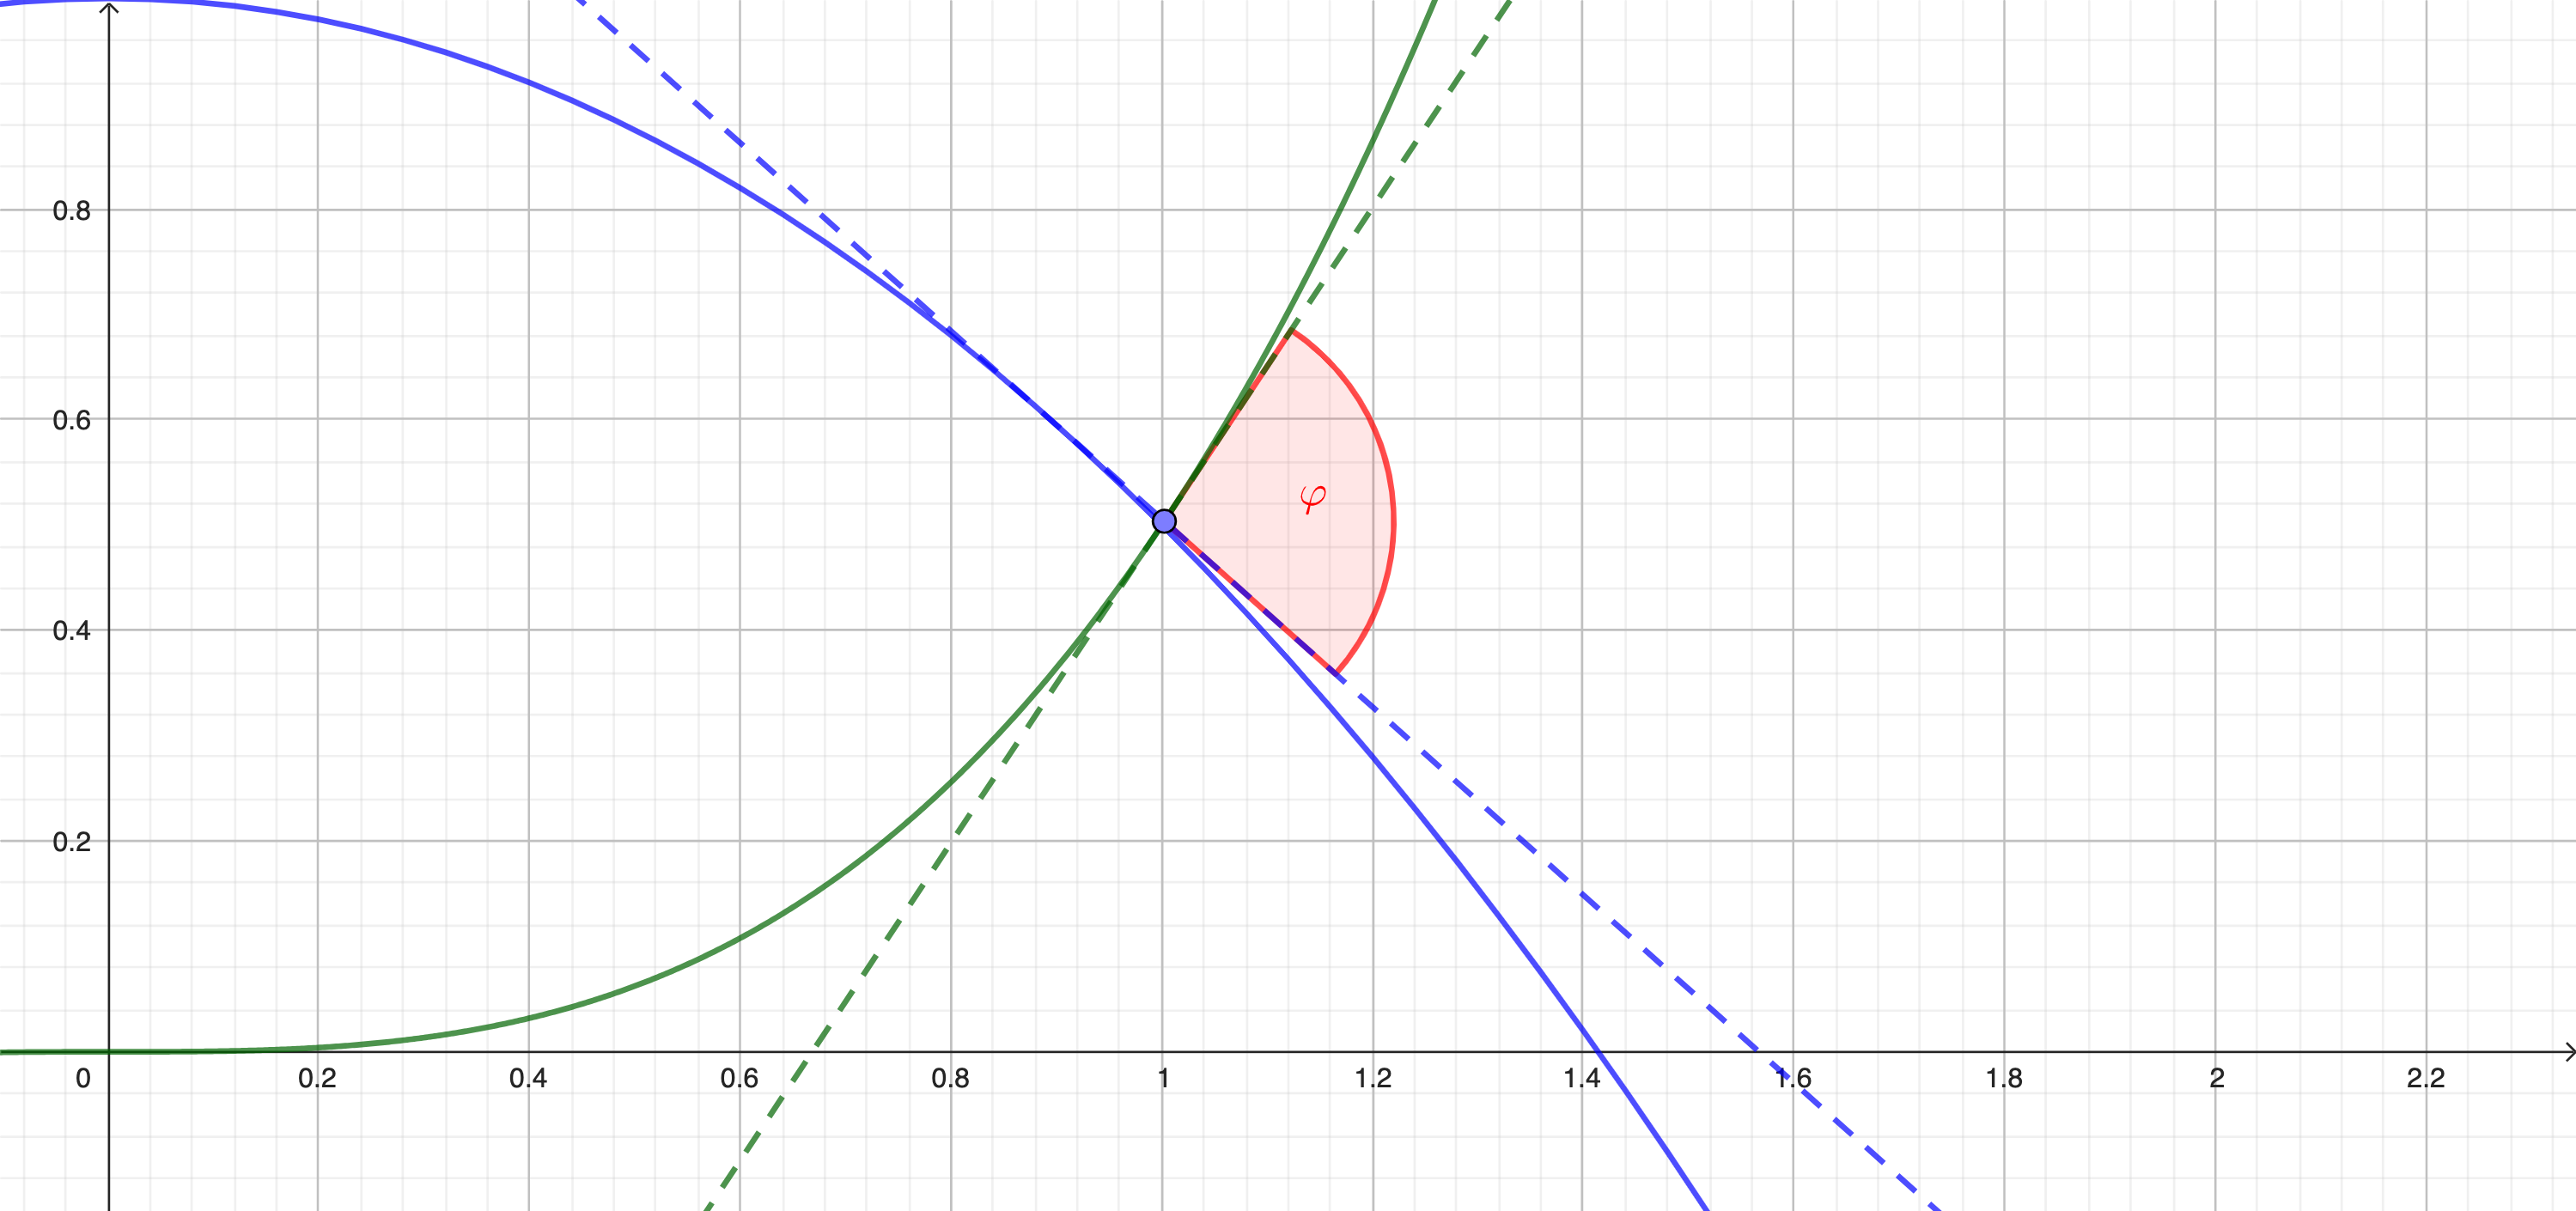
\includegraphics[width = 0.8 \textwidth]{media/WinkelZwKurven.png}
    \end{center}
\end{definition}

Als nächstes stellt sich die Frage, wie der Winkel zwischen zwei Geraden berechnet werden kann. In dem Fall, wo die eine Gerade die $x$-Achse ist, lässt sich der Winkel einfach berechnen. Betrachten Sie dazu die folgende Skizze: 
\begin{center}
    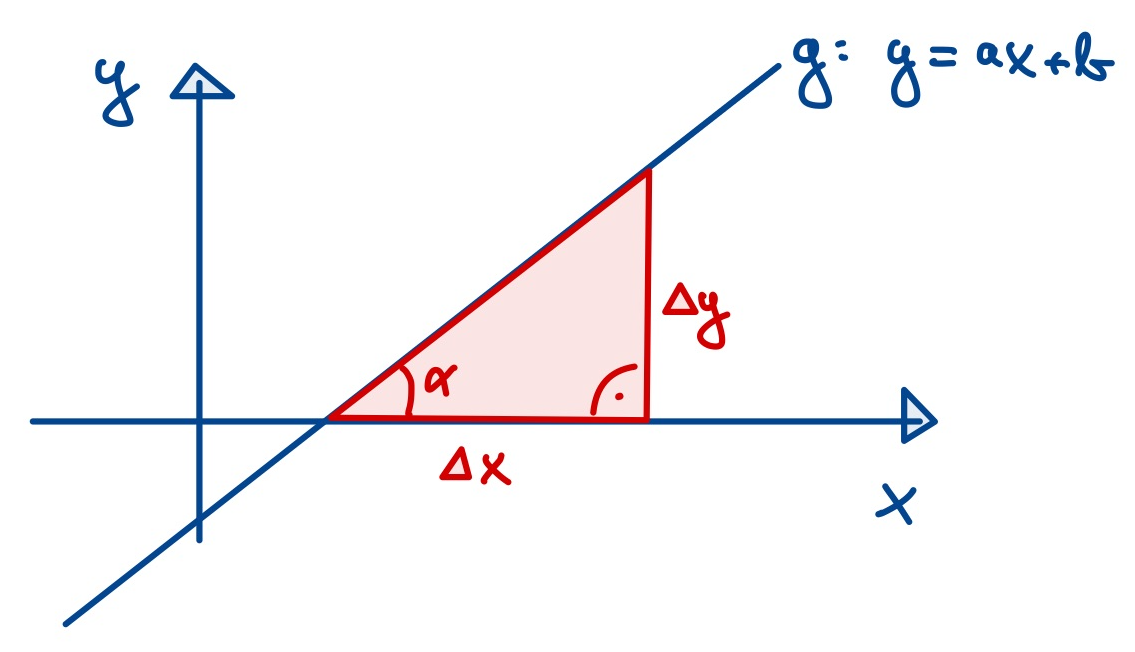
\includegraphics[width = 0.5\textwidth]{media/Winkelx-Achse.png}
\end{center}
Im markierten Steigungsdreieck gilt:
$\tan(\alpha)=\frac{\Delta y}{\Delta x}$
Das Verhältnis $\frac{\Delta y}{\Delta x}$ entspricht der Steigung $a$ der Geraden. Also
$\tan(\alpha) = a$
Damit folgt
$$\alpha = \arctan(a)$$
Im Allgemeinen kann der Winkel zwischen zwei Geraden mit folgender Überlegung berechnet werden:
\begin{center}
    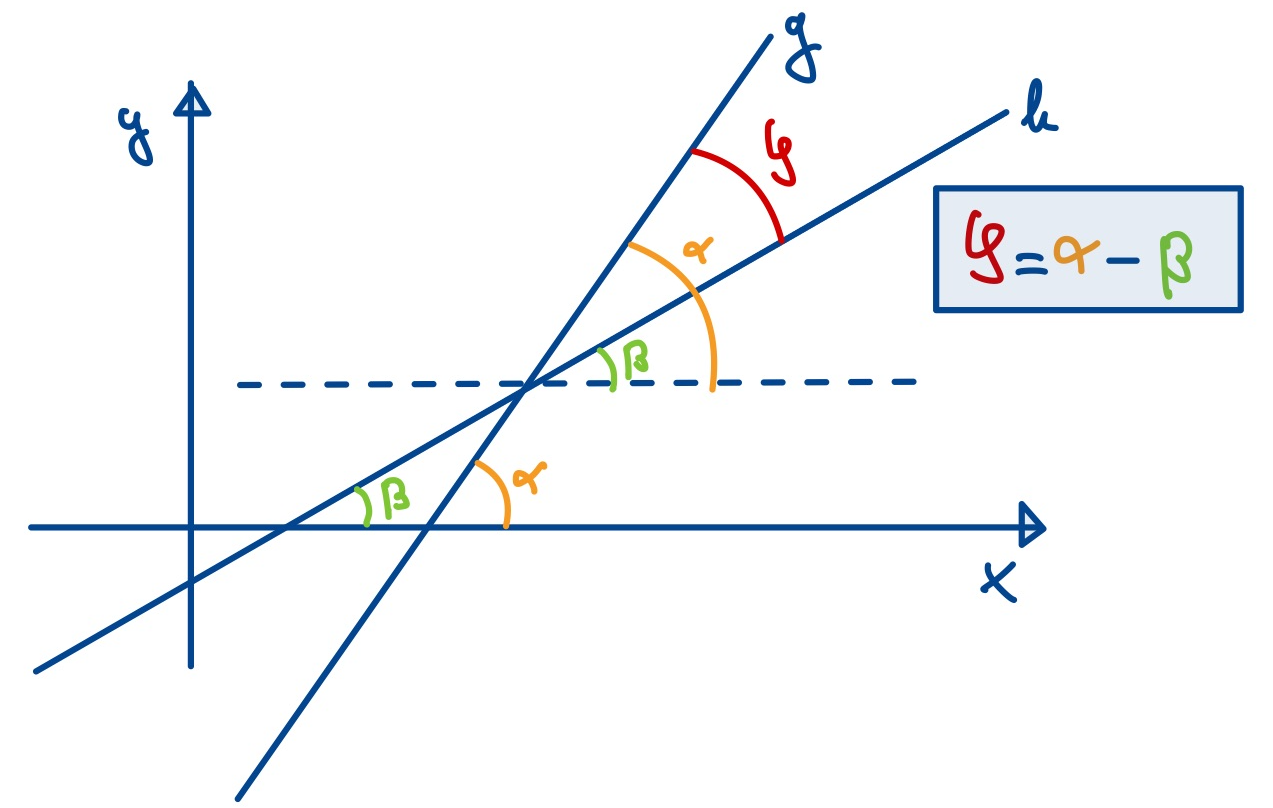
\includegraphics[width = 0.5\textwidth]{media/schnittwinkelZweiGeraden.png}
\end{center}
Zusammengefasst erhalten wir den folgenden Satz:
\begin{satz}
    {Winkelberechnungen}{}
    Der Winkel zwischen zwei Geraden $g:\,   y=a_1 x+b_1$ und $h: y=a_2 x+b_2$ ist
$$\varphi = | \arctan(a_1) - \arctan(a_2) | $$

Der Winkel zwischen den Kurven $y=f(x)$ und  $y=g(x)$, die sich an der Stelle $x_0$ schneiden, ist
$$\varphi = | \arctan(f'(x_0)) - \arctan(g'(x_0)) | $$

\end{satz}

Bemerkungen:
\begin{itemize}
    \item 	Zwei Geraden stehen genau dann senkrecht aufeinander, wenn $a_1 \cdot a_2=-1$ gilt. Entsprechend stehen zwei Kurven genau dann senkrecht aufeinander, wenn an der Schnittstelle $x_0$ gilt $f'(x_0) \cdot g'(x_0)=-1 $.
    \item Die Senkrechte einer Tangente im Berührungspunkt heisst \emph{Kurvennormale}.
    \item Die Formel von oben gilt auch im Fall, dass eine (oder beide) Steigungen negativ sind.
\end{itemize}

\begin{bsp}
    {Berechnung des Schnittwinkels}{}
    In welchem Winkel schneiden sich die Graphen von $f(x)=x^2+2x$ und $g(x)=-x^2-x$?

    % \begin{enumerate}
    %     \item Schnittstellen bestimmen:
    %     $$f(x)=g(x) \iff x^2+2x = -x^2-x \iff 2x^2+3x= 0 \iff x(2x+3) = 0 $$
    %     Die Graphen schneiden sich an den Stellen $x=0$ und $x=-\frac{3}{2}$.

    %     Im Weiteren wird nur der Winkel an der Stelle $x=0$ berechnet.
    %     \item Ableitungen
    %     \begin{align*}
    %         f'(x)=2x+2 &\Rightarrow f'(0) = 2 \\
    %         g'(x)= -2x-1 & \Rightarrow g'(0)=-1
    %     \end{align*}
    %     \item Formel für den Winkel an der Stelle $x=0$
    %     $$ \varphi = \arctan(2)-\arctan(-1) \approx 63.43^\circ -(-45^\circ) =108.43^\circ $$

    % \end{enumerate}

    \vspace*{4cm}

    \phantom{text}


    \clearpage
    \phantom{text}
    
     \vspace*{6cm}

\end{bsp}

% Speziell ist der Fall, wenn zwei Kurven sich rechtwinklig schneiden:

% \begin{satz}
%     {}{}
%     Zwei Kurven $y=f(x)$ und $y=g(x)$, die sich an der Stelle $x_0$ schneiden, stehen senkrecht aufeinander, wenn 

%     $$ g'(x_0) = - \frac{1}{f'(x_0)} $$

% \end{satz}





\begin{ueb}
    {}{}
    \begin{enumerate}
        \item
        Die Parabel \( p \) mit \( y = 2 - \frac{1}{2}x^2 \) schneidet die \( x \)-Achse im Punkt \( R \) rechts vom Ursprung. In diesem Punkt \( R \) wird die Tangente \( t \) an die Parabel \( p \) gelegt und die Normale \( n \) zur Parabel \( p \) errichtet.
        \begin{enumerate}
            \item In welchen Punkten \( T \) und \( N \) schneiden die Tangente \( t \) bzw. die Normale \( n \) die \( y \)-Achse?
            \item In welchem Punkt \( S \) schneidet die Normale \( n \) die Parabel \( p \) ein zweites Mal?
            \item In welchem Winkel schneidet die Parabel die $x$-Achse?
        \end{enumerate}
     \item
        Berechne die Schnittwinkel der folgenden Kurven

        
                \begin{enumerate}
                    \item \( k_1: y = f(x) = \cos(x), \quad k_2: y = g(x) = \sin(x), \quad 0 \leq x \leq \dfrac{\pi}{2} \). \\
                    (Tipp zur Schnittstelle: Teile die Gleichung durch $\cos(x)$)
                    \item \( k_1: y = f(x) = \dfrac{2}{x^2 + 1} \), \quad
                        \( k_2: y = g(x) = x^2 \). \\
                        (Tipp zur Schnittstelle: Substituiere $u=x^2$)
                    % \item \( y = k_1(x) = \dfrac{3 - x}{(x - 2)^2} \), \quad
                    %     \( y = k_2(x) = x - 3 \)
                    \item \( y = k_1(x) = e^{-\frac{x + 1}{2}} \), \quad
                        \( y = k_2(x) = e^{-x^2} \)
                    \item \( y = k_1(x) = \ln(x + 3) \), \quad
                        \( y = k_2(x) = \ln(7 - x) \)
                \end{enumerate}


\item Für welchen Wert des positiven Koeffizienten \( a \) schneiden sich die beiden Graphen der Funktionen
\[
f(x) = ax^2 \quad \text{und} \quad g(x) = \frac{1}{x}
\]
orthogonal, d.\,h.\ rechtwinklig?



    \end{enumerate}
\end{ueb}


\clearpage
\emph{Lösungen:}
\begin{enumerate}
    \item
    \begin{enumerate}
        \item \( T = (0, 4), \quad N = (0, -1) \)
        \item \( S = (-3, -2.5) \)
        \item \( \varphi \approx 63.4^\circ \)
    \end{enumerate}

    \item
    \begin{enumerate}
        \item \( \varphi \approx 70.5^\circ \)
        \item \( \varphi_1 = \varphi_2  \approx 71.6^\circ \)
        \item \( \varphi_1 \approx 25.9^\circ \quad \varphi_2  \approx 59.2^\circ\)
        \item \( \varphi \approx 22.6^\circ \)
    \end{enumerate}

    \item \( a = \dfrac{1}{2} \sqrt[4]{2} \approx 0.6\)
\end{enumerate}


\clearpage
\subsection{Spezielle Punkte und Eigenschaften von Kurven}
\label{speziellePte}
\subsubsection{Extrema und Wendepunkte bestimmen}
\begin{LA}
    {Zuordnung von Graphenausschnitten}{zuordnungGraphen}
    In den Koordinatensystemen oben sind Ausschnitte von sechs Funktionsgraphen gezeichnet. In den Koordinatensystemen unten Ausschnitte von sechs Ableitungen. Welcher Ableitung passt zu welchem Graph?


    \begin{center}
        
    
    \begin{tabular}{|c|c|c|}
        \hline
        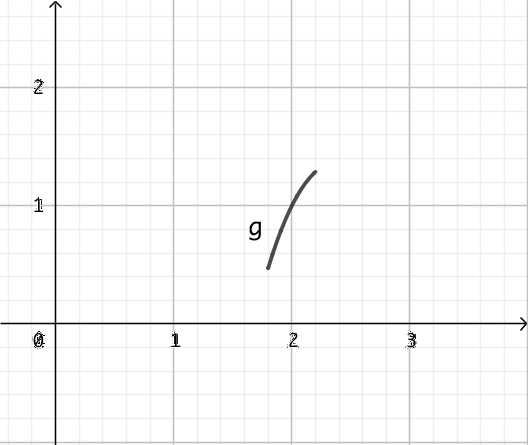
\includegraphics[width = 4cm]{media/Graph und Ableitung Kopie/Graph 1.png} &
        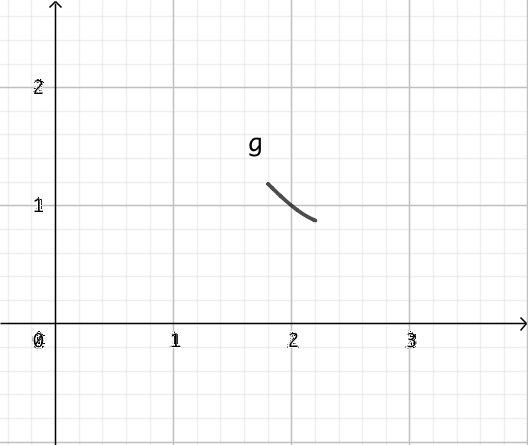
\includegraphics[width = 4cm]{media/Graph und Ableitung Kopie/Graph2.png} &
        \includegraphics[width = 4cm]{media/Graph und Ableitung Kopie/Graph3.png} \\  \hline

        \includegraphics[width = 4cm]{media/Graph und Ableitung Kopie/Graph4.png} & 
        \includegraphics[width = 4cm]{media/Graph und Ableitung Kopie/Graph5.png} & 
        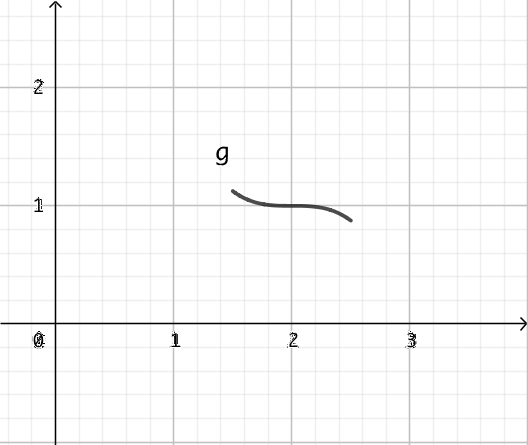
\includegraphics[width = 4cm]{media/Graph und Ableitung Kopie/graph6.png} \\ \hline
        \hline

        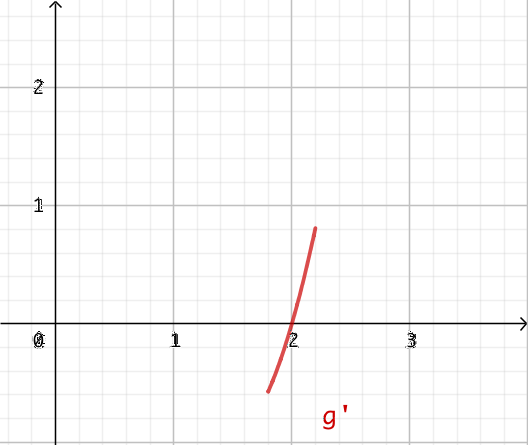
\includegraphics[width = 4cm]{media/Graph und Ableitung Kopie/ableitung 4.png} &
        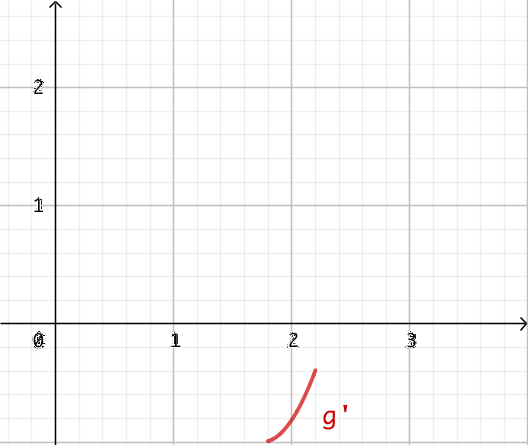
\includegraphics[width = 4cm]{media/Graph und Ableitung Kopie/Ableitung 2.png} &
        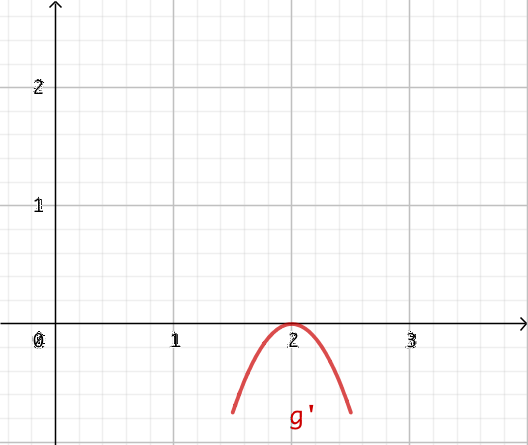
\includegraphics[width = 4cm]{media/Graph und Ableitung Kopie/ableitung6.png} \\ \hline

        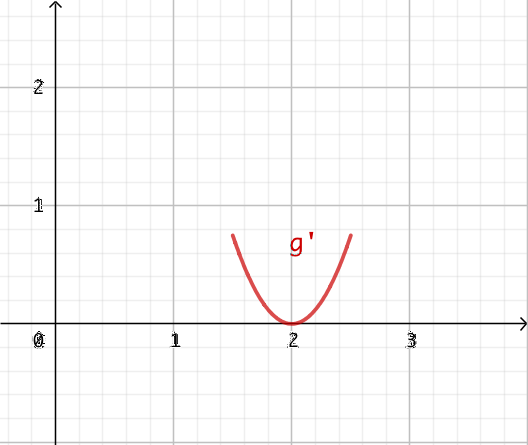
\includegraphics[width = 4cm]{media/Graph und Ableitung Kopie/ableitung5.png} & 
        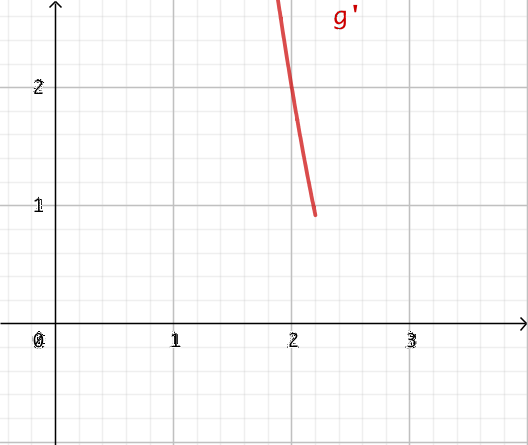
\includegraphics[width = 4cm]{media/Graph und Ableitung Kopie/ableitung 1.png} & 
        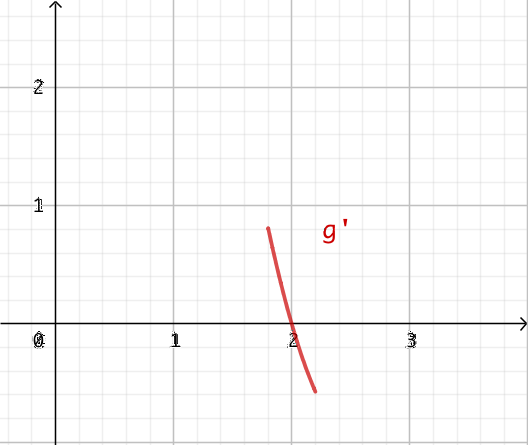
\includegraphics[width = 4cm]{media/Graph und Ableitung Kopie/ableitung3.png} \\ \hline
    \end{tabular}
\end{center}



\end{LA}
\clearpage

Aufgrund des Vorzeichens der ersten Ableitung einer Funktion kann man Rückschlüsse auf die Gestalt des ursprünglichen Graphen ziehen. Erste Erkenntnisse aus der Lernaufgabe \ref{LA:zuordnungGraphen} lassen sich wie folgt zusammenfassen:

Sei $f$ eine differenzierbare Funktion mit Definitionsbereich $\DD_f$. Sei $I \subset \DD_f$ ein Intervall und $x_0 \in \DD_f$. Dann gilt:

\begin{center}
    \begin{tabular}{| m{10cm} | m{4cm}|} \hline
        $f$ ist im Intervall $I$ \emph{monoton wachsend} $$\iff$$ $ f'(x)\ge 0$ für alle $x\in I$ & 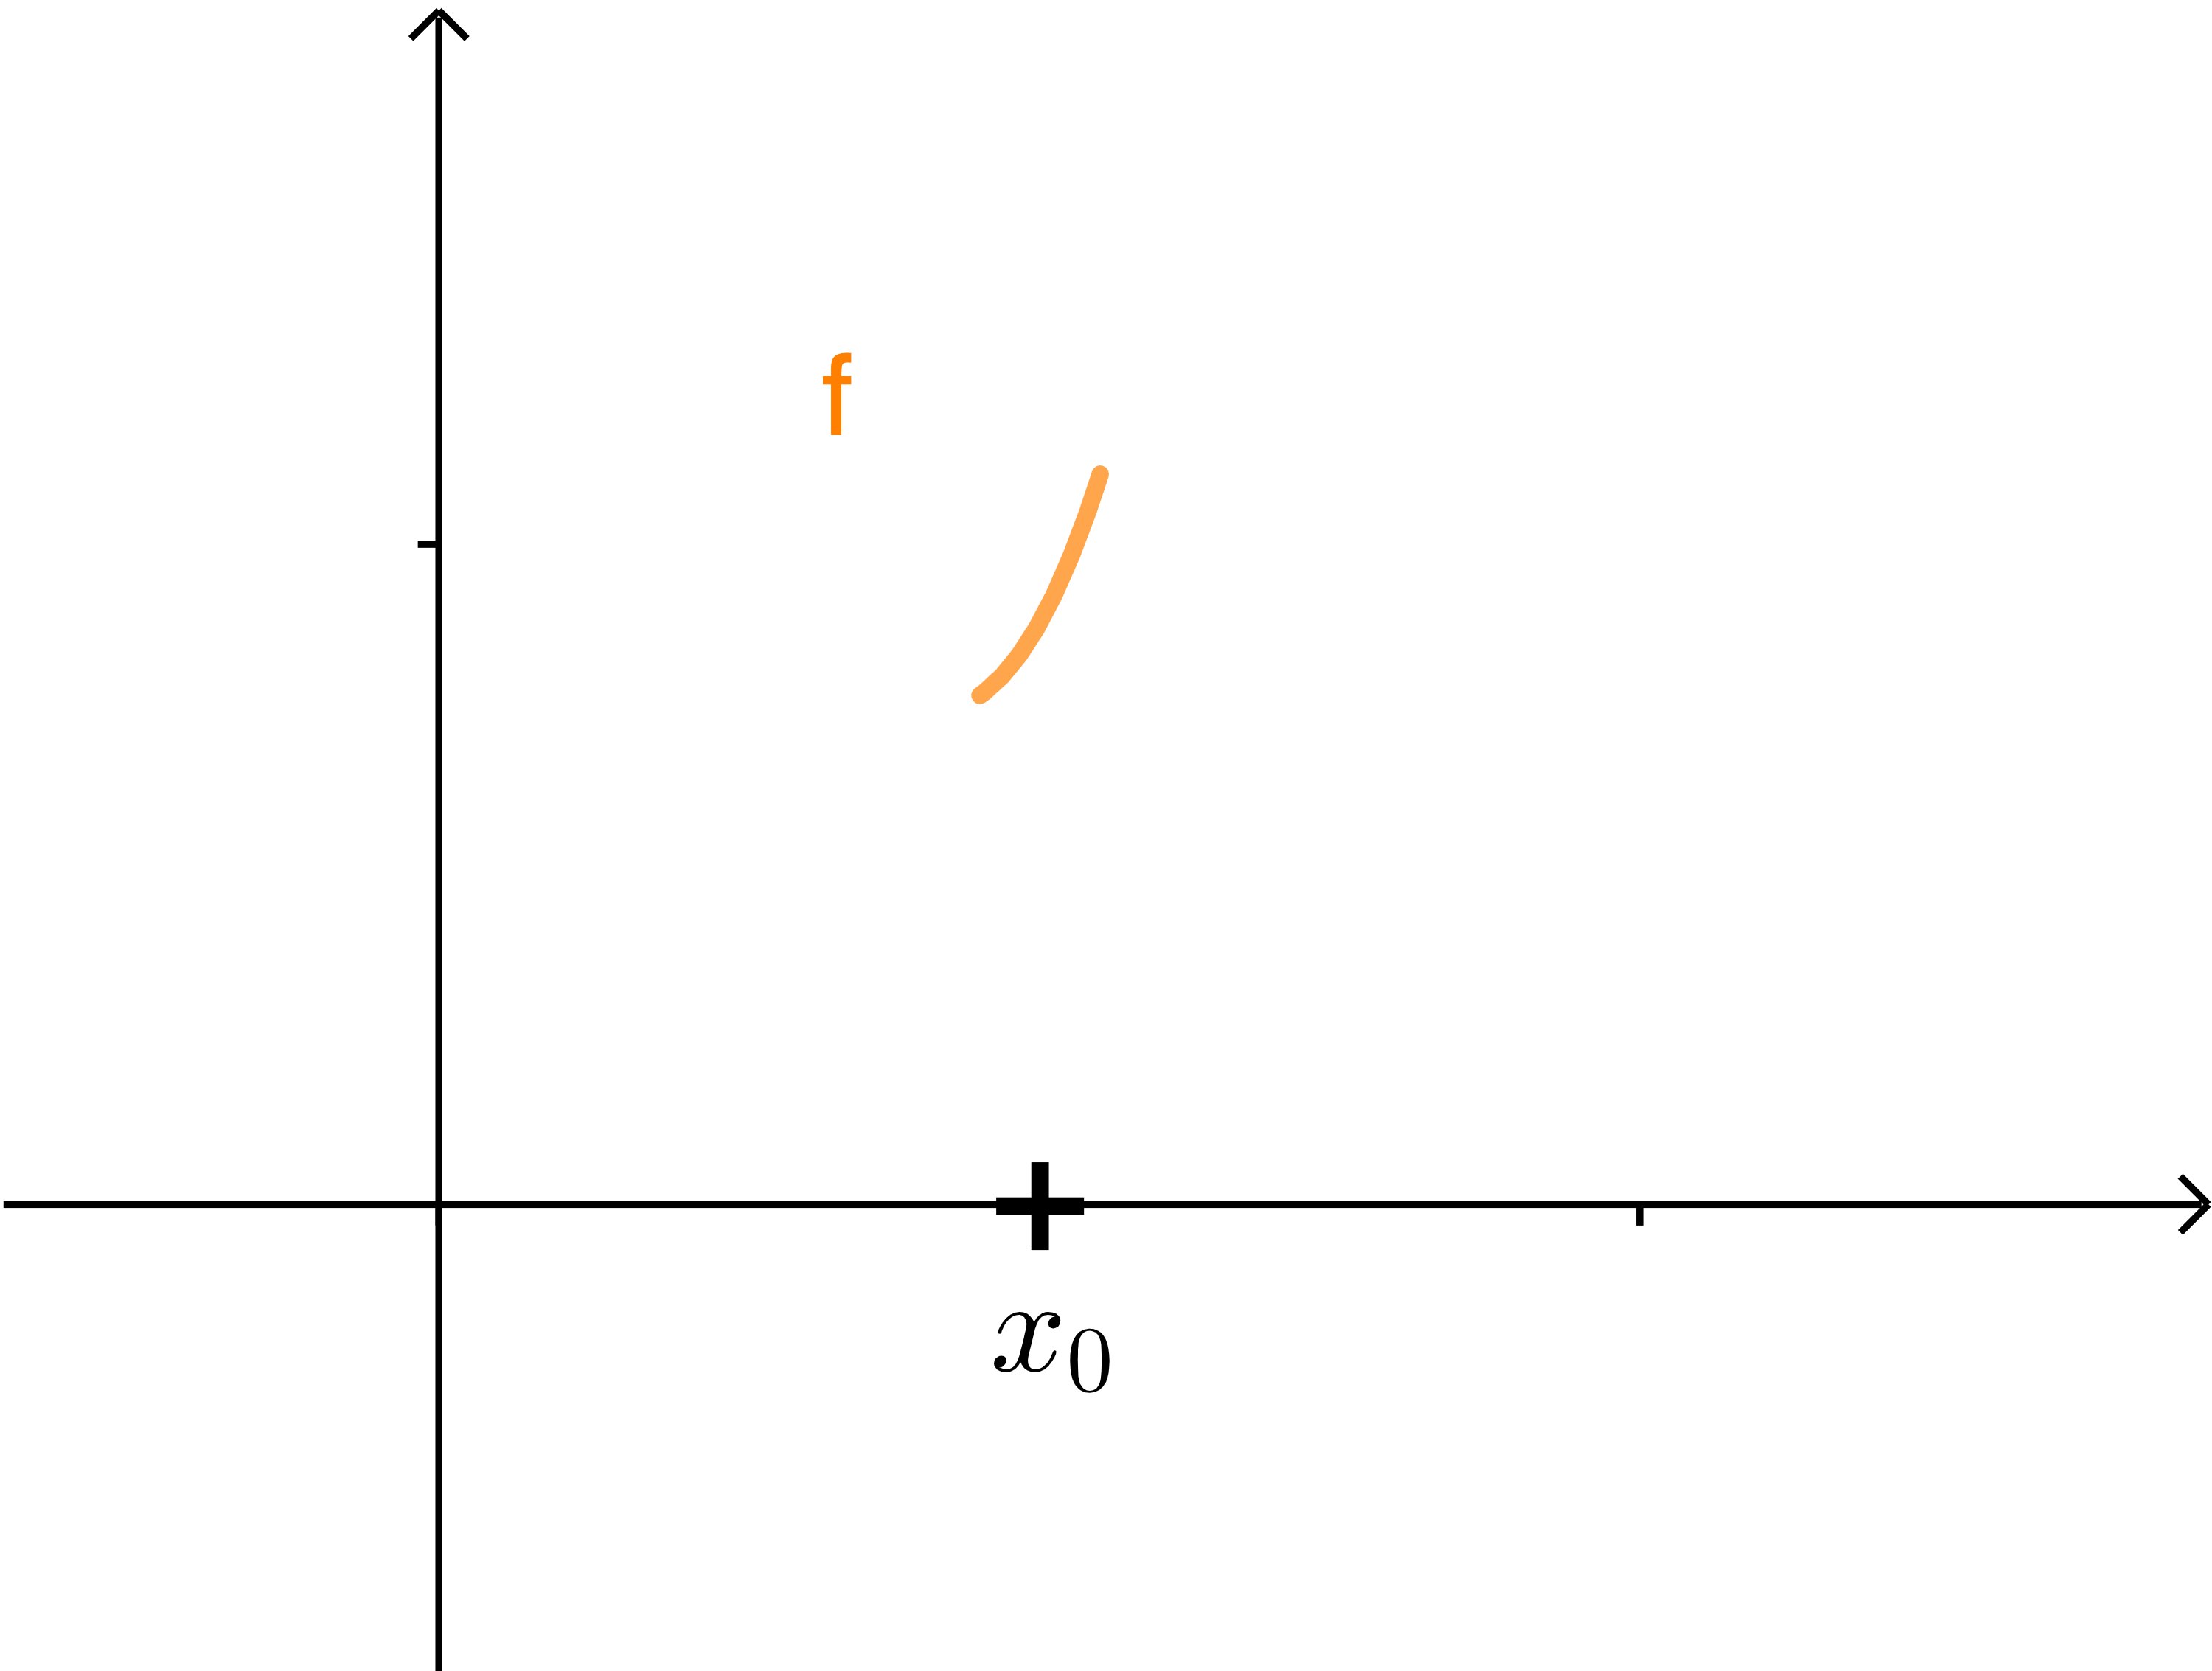
\includegraphics[width = 4cm]{media/Graph und Ableitung Kopie/wachsend.png}\\ \hline
        $f$ ist im Intervall $I$ \emph{monoton fallend} $$\iff$$  $f'(x) \le 0$ für alle $x\in I$ &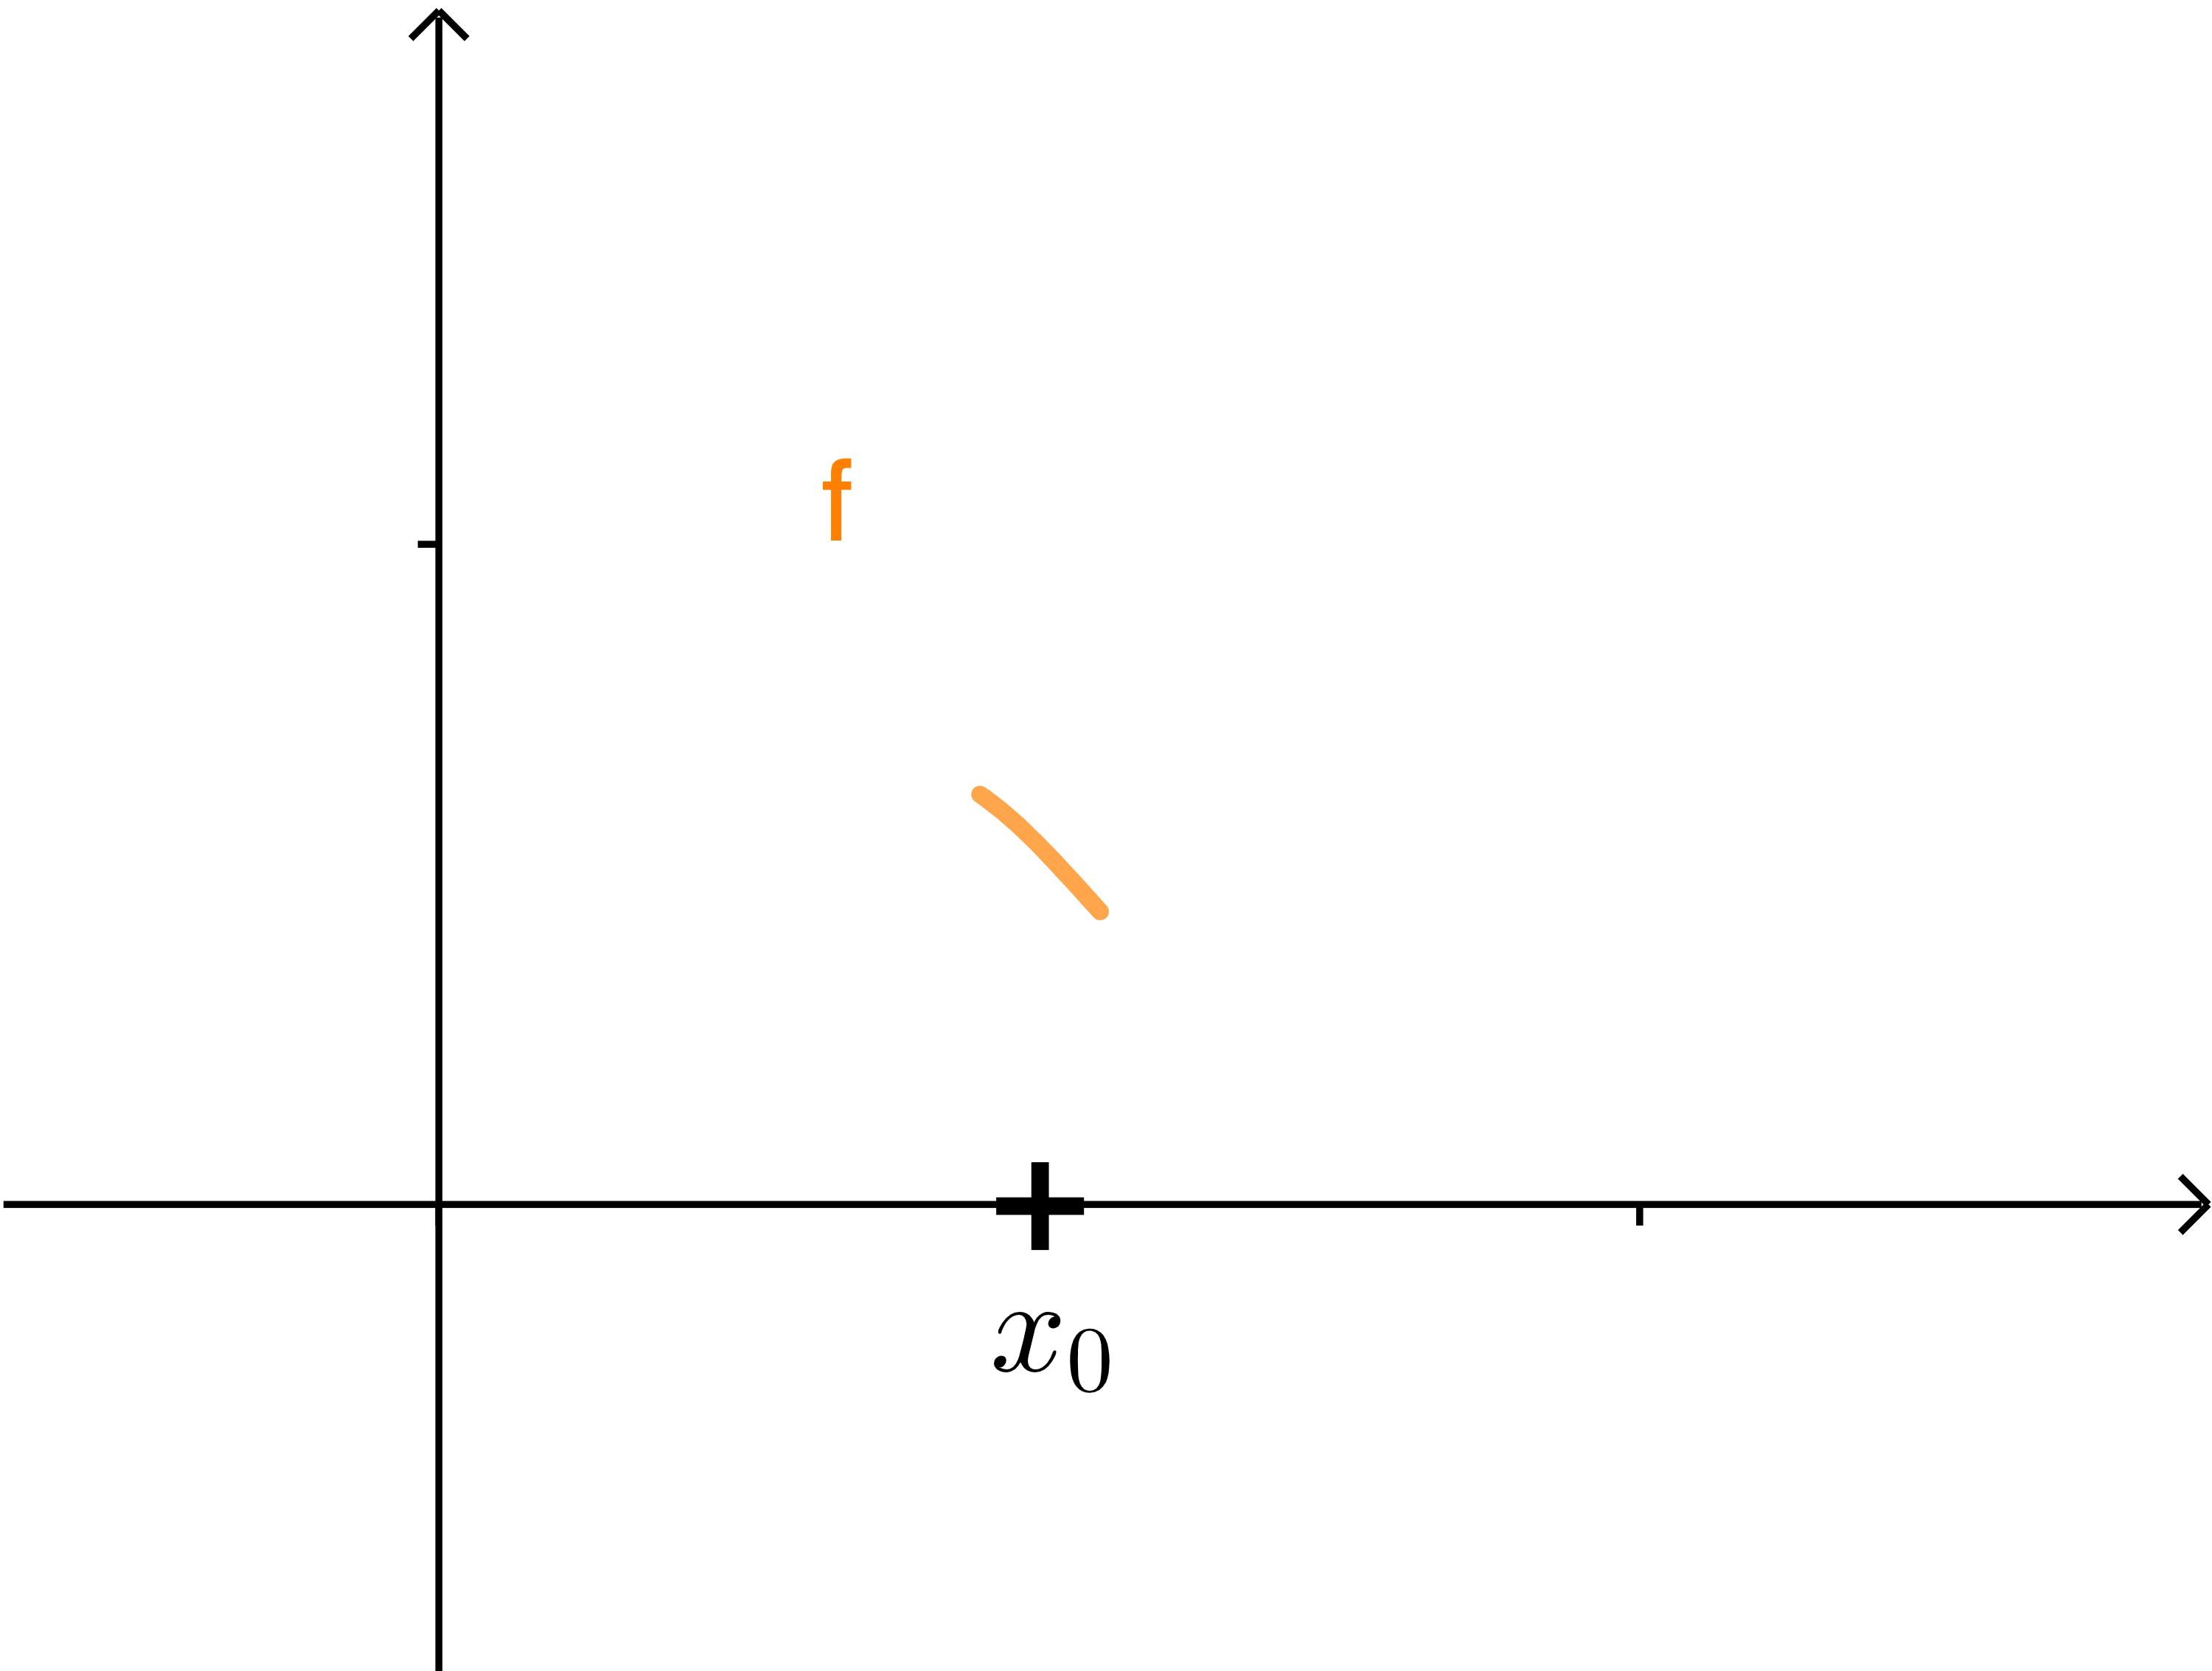
\includegraphics[width = 4cm]{media/Graph und Ableitung Kopie/fallend.png}\\ \hline
        $f$ hat an der Stelle $x_0$ ein \emph{lokales Maximum} (auch Hochpunkt genannt) $$\iff$$ $f'$ wechselt an der Stelle $x_0$ das Vorzeichen von positiv zu negativ. & 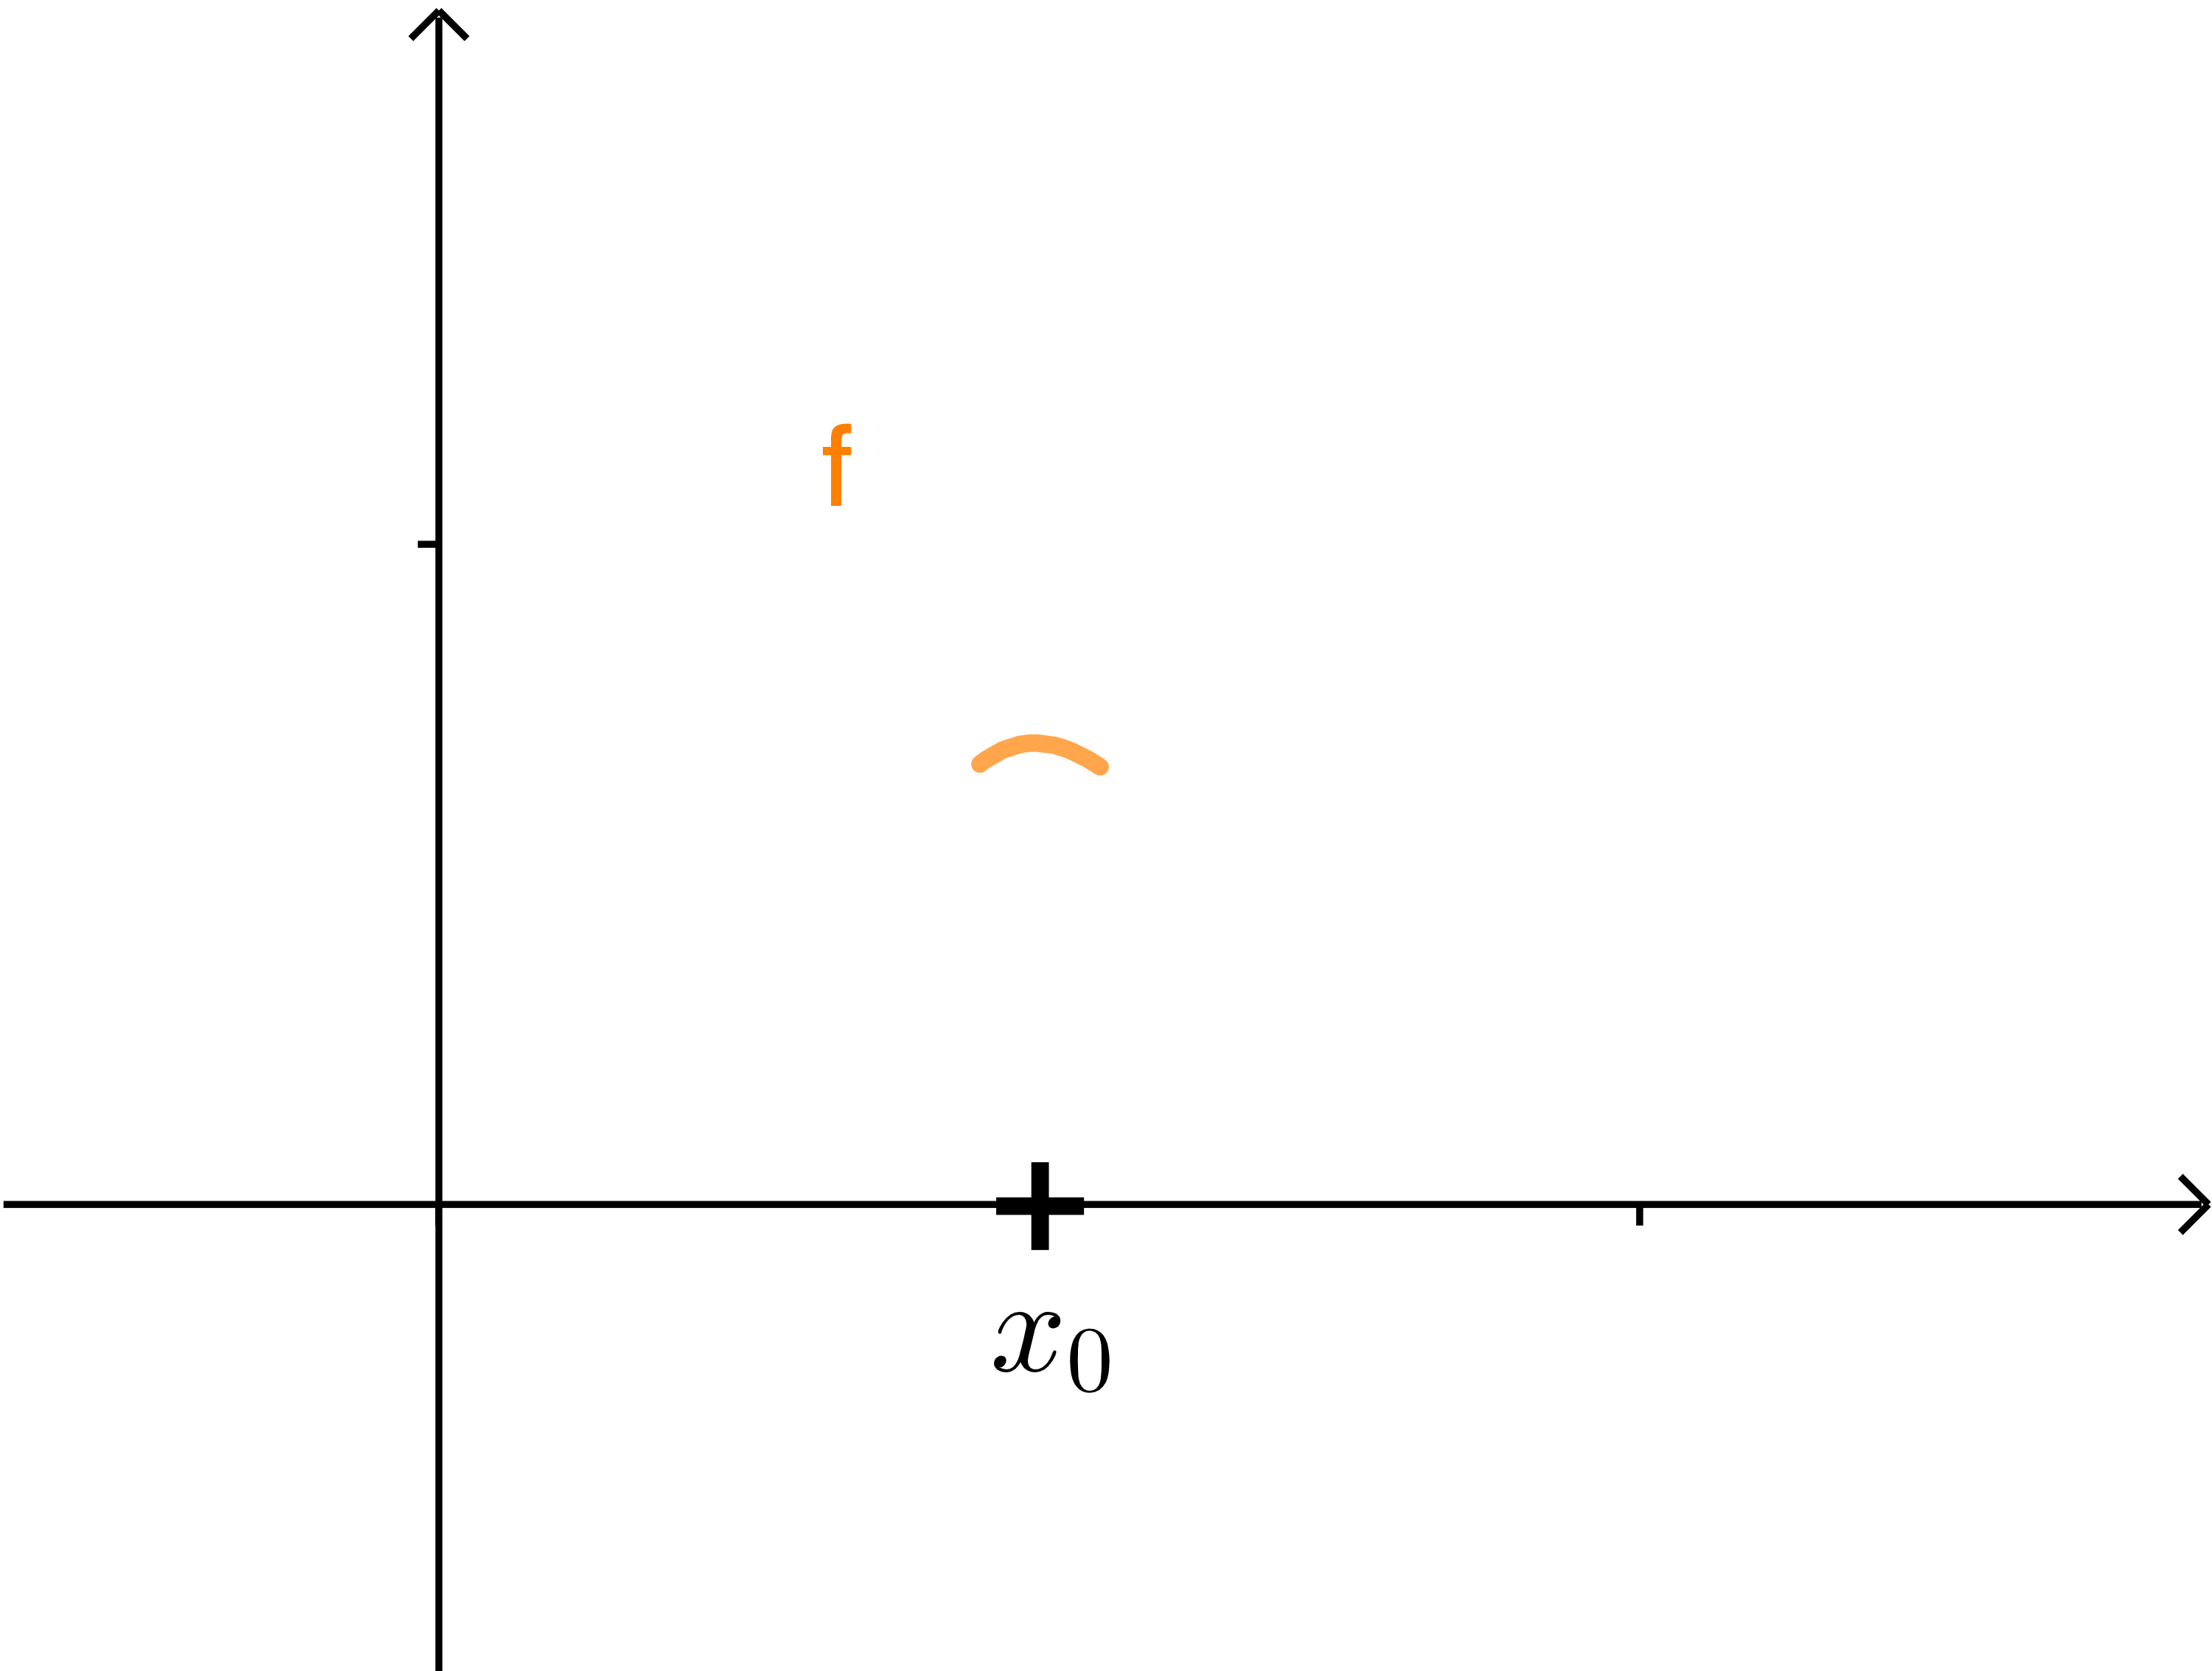
\includegraphics[width = 4cm]{media/Graph und Ableitung Kopie/maxx.png} \\ \hline
        $f$ hat an der Stelle $x_0$ ein \emph{lokales Minimum} (auch Tiefpunkt genannt) $$\iff$$  $f'$ wechselt an der Stelle $x_0$ das Vorzeichen von negativ zu positiv. & 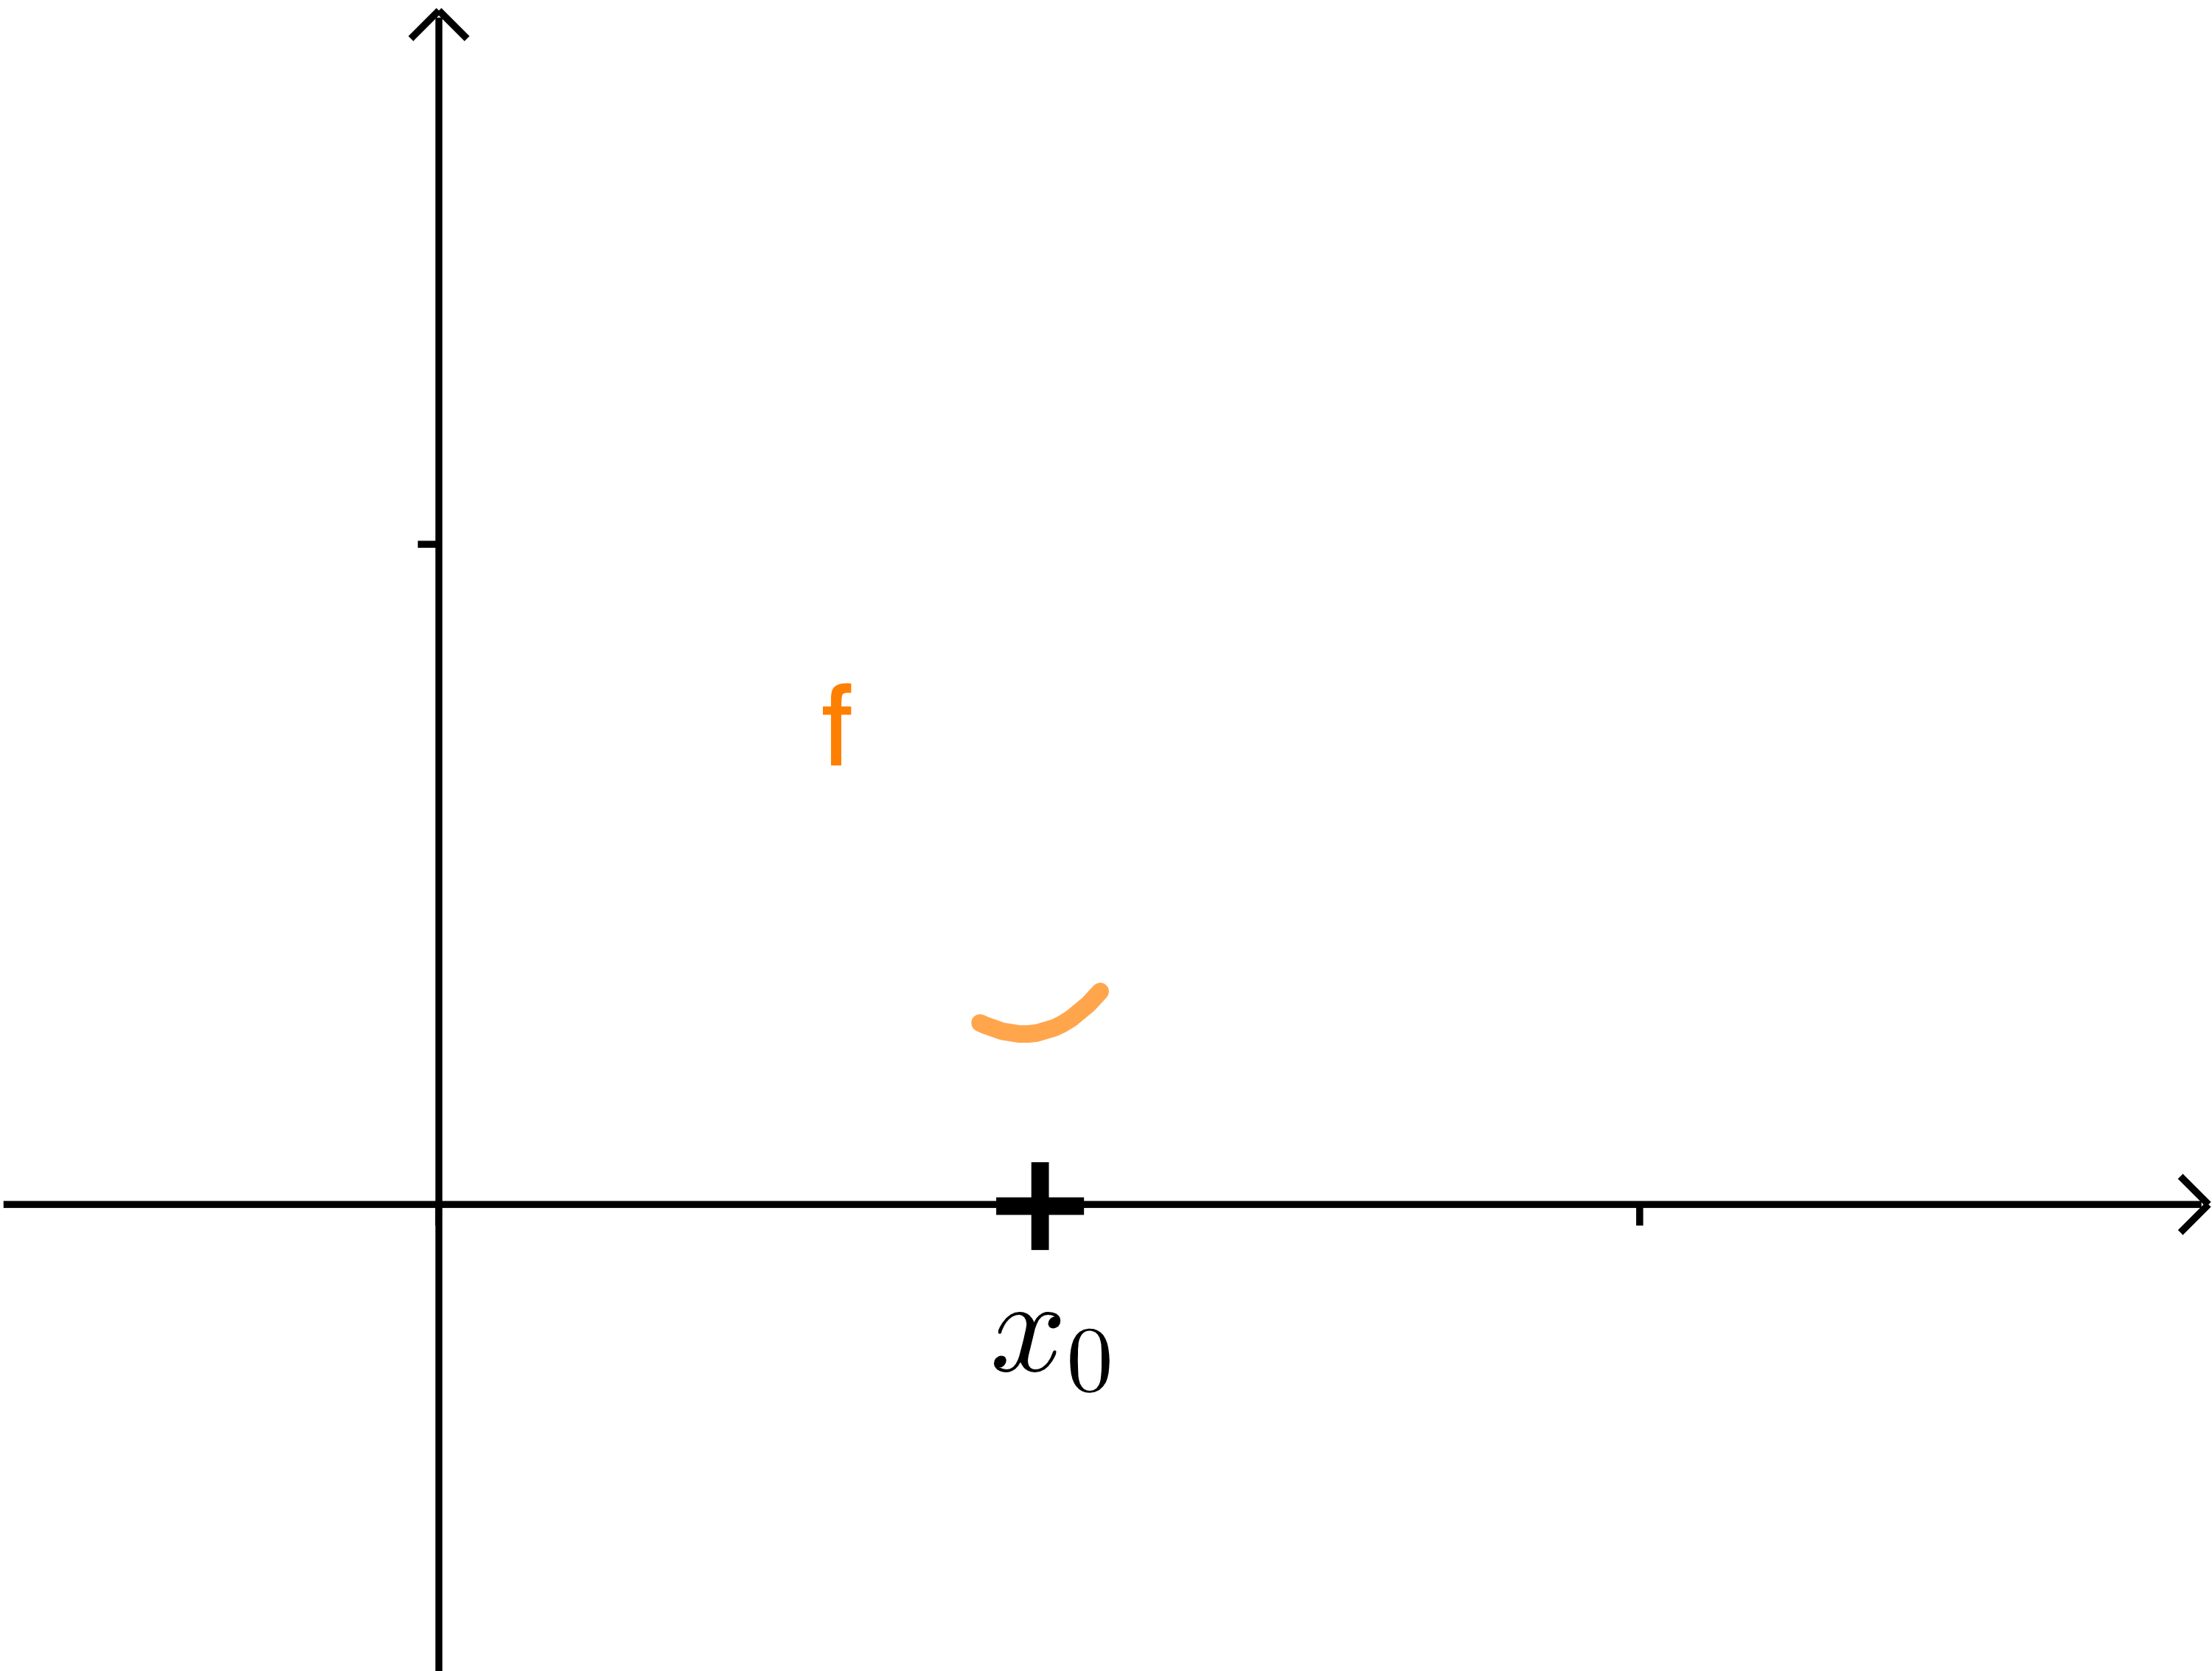
\includegraphics[width = 4cm]{media/Graph und Ableitung Kopie/min.png}\\ \hline
    \end{tabular}
\end{center}

Der Nachweis, dass eine Ableitungsfunktion $f'$ das Vorzeichen an einer bestimmen Stelle von $+$ nach $-$ oder umgekehrt wechselt, kann in der Praxis kompliziert sein. Häufiger ist es einfacher, wenn man dazu die Ableitungsfunktion $f'$ nochmals ableitet!

% \begin{definition}
%     {Höhere Ableitung}{}
%     Sei $f'$ die Ableitung einer Funktion $f$. Wenn $f'$ selbst wieder differenzierbar ist, bezeichnet man die Ableitung von $f'$ mit $f''$ und man nennt sie die zweite Ableitung von $f$.

%     Von der Funktion $f''$ lässt sich die sogenannte dritte Ableitung $f'''$ bilden u.s.w.

%     Die $n$-te Ableitung bezeichnet man mit $f^{(n)}$.

%     Einealternative Notation für die zweite, dritte und $n$-te Ableitung ist: $\frac{d^2}{dx^2}, \frac{d^3f}{dx^3}, \frac{d^nx}{dx^n}$
% \end{definition}

% \begin{bsp}
%     {Ableitungen von $f(x) = 3x^4+2x-1$}{}
%     $ f'(x) = 12x^3+2 \Rightarrow f''(x) = 36x^2 \Rightarrow f'''(x) = 72x \Rightarrow f^{(4)}(x) = 72 \Rightarrow f^{(5)}(x) = 0 \Rightarrow f^{(6)}(x) = 0, \dots$
% \end{bsp}







Wie kann man nun mit den höheren Ableitungen entscheiden, ob $f'$ an einer bestimmten Stelle das Vorzeichen von $+$ nach $-$ oder umgekehrt wechselt? Betrachten Sie dazu das folgende Beispiel:
\clearpage

\begin{bsp}
    {Von der Ableitung zum Funktionsgraphen (wird im Unterricht ergänzt)}{}
    Wie sieht der Graph einer Funktion $f$ in der Umgebung von $x=1$ aus, wenn $f(1)=4,f' (1)=0$ und $f'' (1)=2$ ist?

    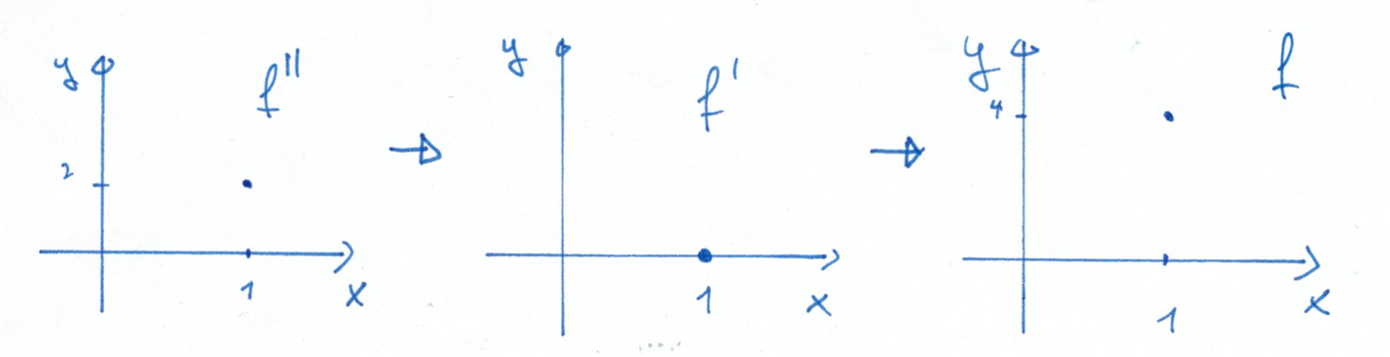
\includegraphics[width = \textwidth]{media/bspAbleitungZuGraph.png}
\end{bsp}

Merke:
\begin{definition}
    {Krümmung des Graphen}{}
    \begin{center}
    \begin{tabular}{| m{10cm} | m{4cm}|} \hline
        $f$ ist im Intervall $I$ \emph{linksgekrümmt (oder konvex)} $$\iff$$ $ f''(x) > 0$ für alle $x\in I$ & \includegraphics[width = 4cm]{media/linksgekrümmt.png}\\ \hline
        $f$ ist im Intervall $I$ \emph{rechtsgekrümmt (oder konkav)} $$\iff$$  $f''(x) < 0$ für alle $x\in I$ &\includegraphics[width = 4cm]{media/rechstgekrümmt.png}\\ \hline
        $f$ hat an der Stelle $x_0$ einen \emph{Wendepunkt} $$\iff$$ $f''$ wechselt an der Stelle $x_0$ das Vorzeichen . & 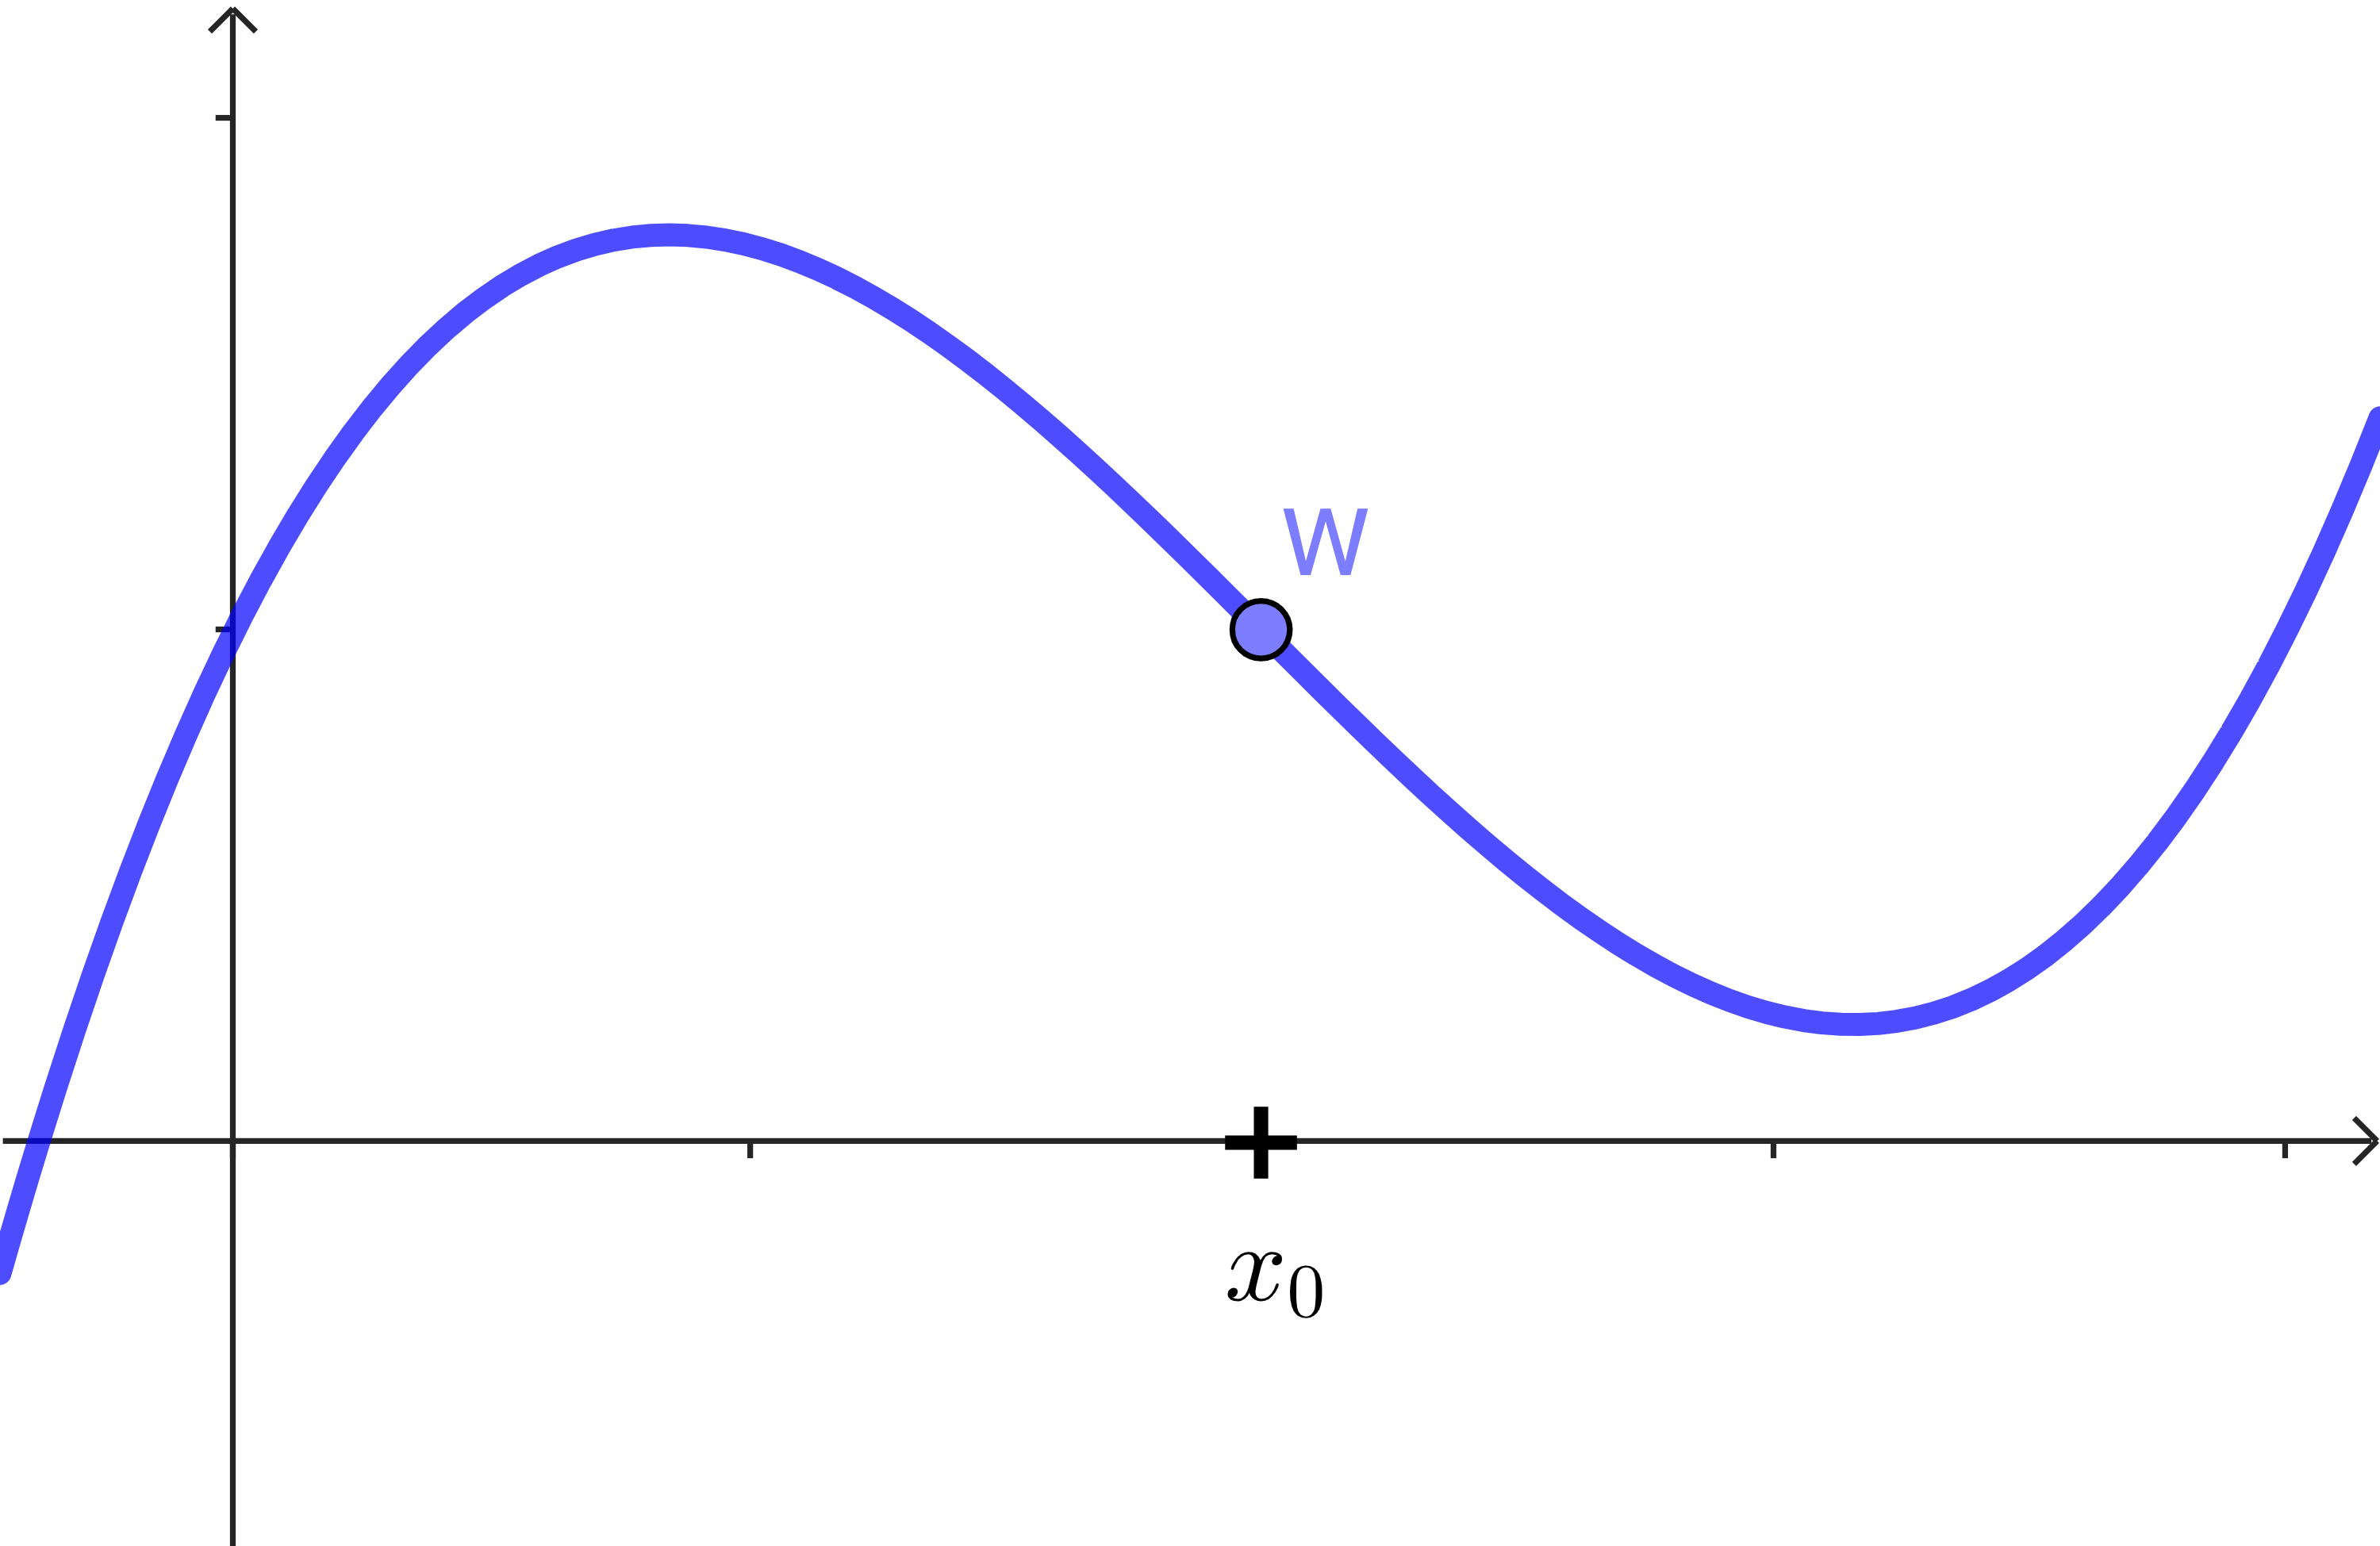
\includegraphics[width = 4cm]{media/wendept-def.png} \\ \hline
        
    \end{tabular}
\end{center}
\end{definition}

\clearpage

\begin{LA}
    {Von der Ableitung zum Funktionsgraphen}{}   
    Versuchen Sie selbst, die Informationen von links nach rechts zu übertragen, und skizzieren Sie den Graphen in einer Umgebung der markierten Punkte (mit Ausnahme der Graphen ganz links)

    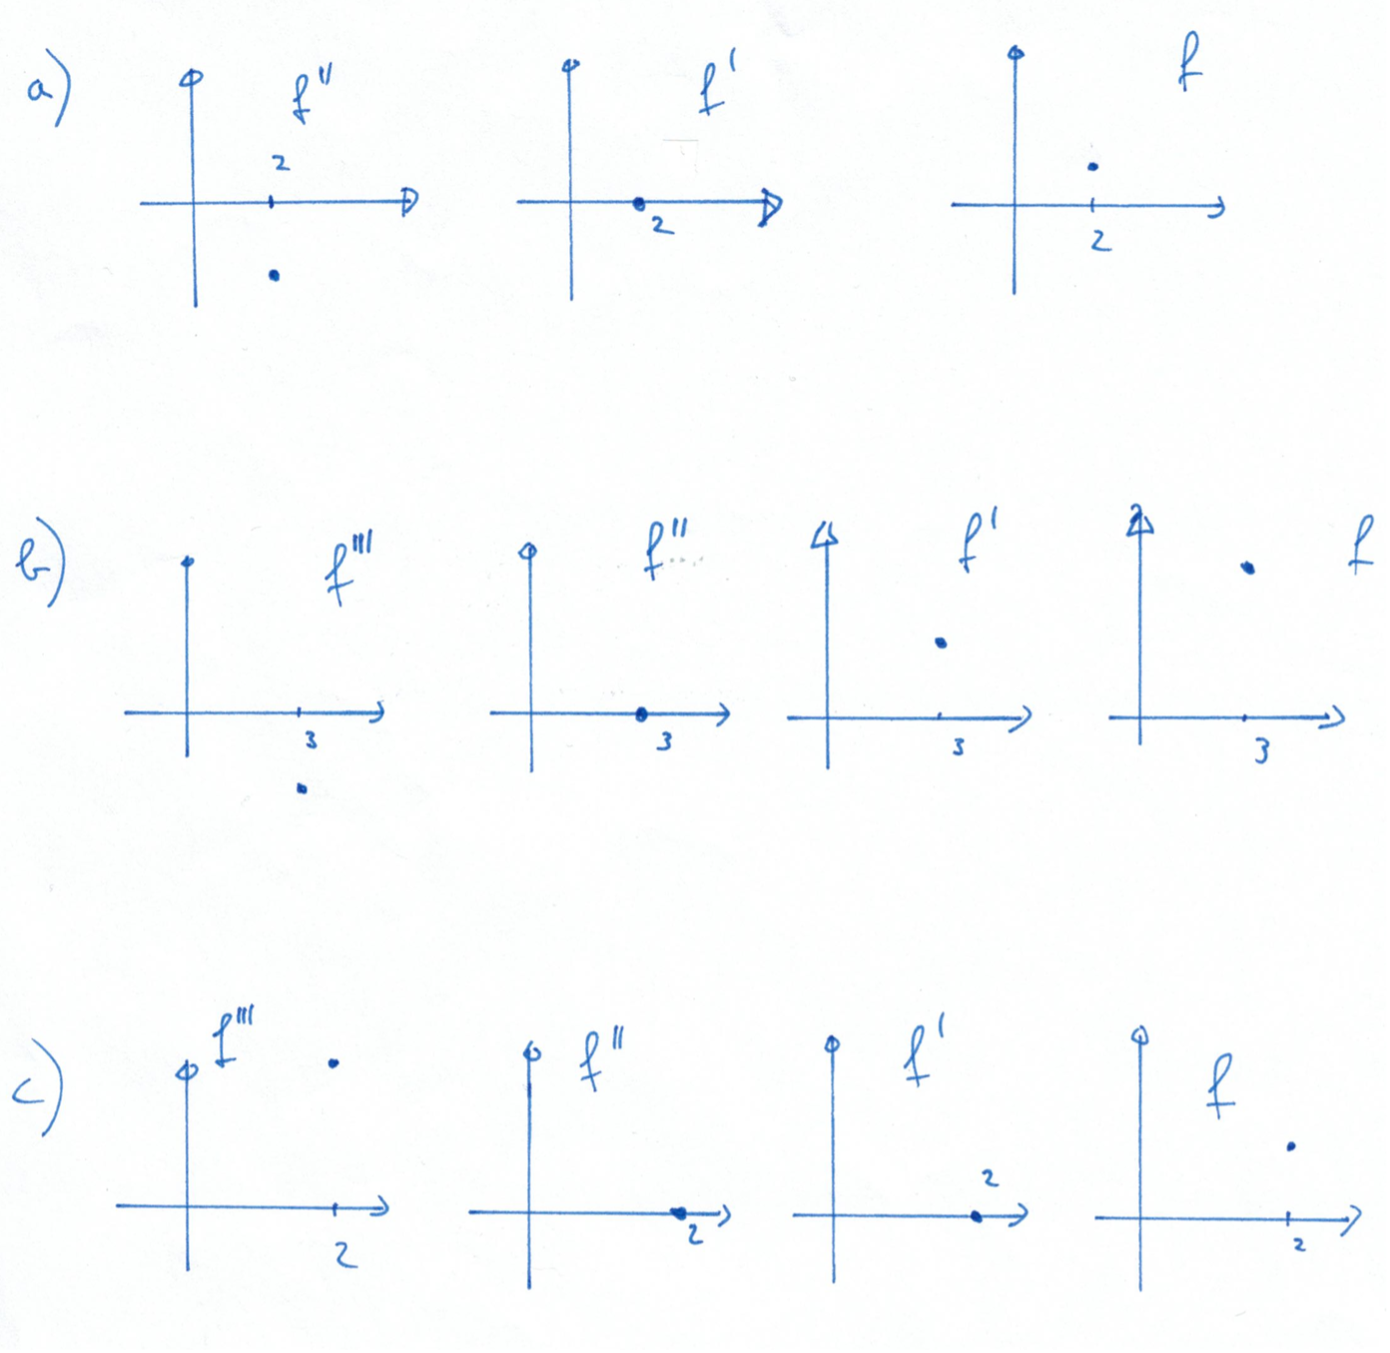
\includegraphics[width = \textwidth]{media/lavonGraphzurFu.png}
\end{LA}

\clearpage

Zusammenfassung: Hinreichende Bedingungen für spezielle Graphenpunkte

\begin{center}
    \begin{tabular}{| m{5cm} | m{5cm} | m{4cm}|} \hline
        \textbf{Hinreichende Bedingung} & \textbf{Art des Punktes} & \textbf{Bild} \\ \hline
        $$f'(x_0) = 0,$$ $$f''(x_0) < 0$$ & Lokales Maximum / Hochpunkt an der Stelle $x_0$ & 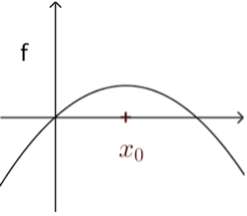
\includegraphics[width = 3.9cm]{media/lokMax.png}\\ \hline
        $$f'(x_0) = 0,$$  $$f''(x_0) > 0$$ & Lokales Minimum / Tiefpunkt an der Stelle $x_0$ & 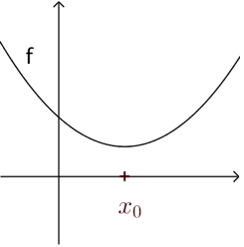
\includegraphics[width = 3.9cm]{media/lokMin.png}\\ \hline
        $$f''(x_0) = 0,$$  $$f'''(x_0) \neq 0$$ & Wendepunkt an der Stelle $x_0$ &  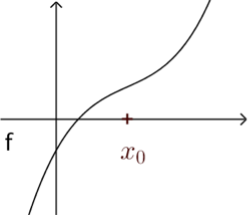
\includegraphics[width = 3.9cm]{media/wendept.png} \\ \hline
        $$f'(x_0) = 0,$$  $$f''(x_0) = 0,$$  $$f'''(x_0) \neq 0 $$ & Sattelpunkt / Terrassenpunkt an der Stelle $x_0$  \linebreak (= Wendepunkt mit horizontaler Tangente) & 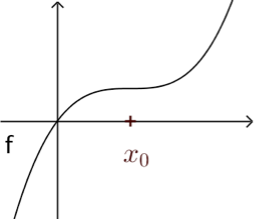
\includegraphics[width = 3.9cm]{media/sattelpt.png} \\ \hline
    \end{tabular}
\end{center}

Die speziellen Graphenpunkte haben je nach Kontext wichtige Bedeutungen. So sind z.B. Hochpunkte von Gewinnfunktionen besonders interessant, da sie den maximalen Gewinn angeben. Wendepunkte sind in der Physik oft mit einem Richtungswechsel einer Bewegung verbunden. Einige dieser Anwendungen werden wir später genauer untersuchen. Für den Moment wollen wir uns auf die mathematische Bestimmung dieser Punkte konzentrieren.
\clearpage
\begin{bsp}
{}{}
Hat die Funktion $f(x) = \frac{8}{x} -\frac{16}{x^2}$ einen Hoch- oder Tiefpunkt?

\vspace*{20 cm}
\end{bsp} 


\clearpage
Was bedeutet \emph{hinreichend}? Am Beispiel des lokalen Maximums bedeutet es das Folgende: Wenn $f'(x_0)=0$ und $f'' (x_0 )<0$ dann hat die Funktion an der Stelle $x_0$ mit Sicherheit ein lokales Maximum. \textbf{Umgekehrt aber nicht}: Wenn die Funktion an der Stelle $x_0$ ein lokales Maximum hat, dann folgt nicht unbedingt, dass die zweite Ableitung negativ ist: $f''(x_0)$ könnte auch $0$ sein.
%  Es gilt
%     $$f'(x_0) = 0, f''(x_0) > 0 \quad \Longrightarrow \text{ Tiefpunkt bei } x_0$$
%     aber
%     $$\text{ Tiefpunkt bei } x_0 \quad \cancel\Longrightarrow  \quad f'(x_0) = 0, f''(x_0) > 0 $$

\begin{bsp}
    {Hinreichende vs. notwendige Bedingungen}{hinreichendNotwendig}
    Untersuche die Funktion $f(x) = x^4-1$

    \vspace*{18cm}

\end{bsp} 

\clearpage

\begin{ueb}
    {}{}
    \begin{enumerate}
        \item Bestimme die Extrema (= Hoch- und Tiefpunkte) der Funktion  $$ f(x) = x^3 + 6x^2 - 15x + 19$$
        \item  Gegeben ist die Funktion \( f \) mit \( f(x) = x^3 + 3x^2 - 4 \).
        \begin{enumerate}
            \item Bestimme vom Graphen der Funktion \( f \) alle Tief-, Hoch- und Wendepunkte.
            \item Gib jeweils die Intervalle an, in welchen der Graph der Funktion \( f \) monoton steigt bzw. fällt.
            \item Skizziere den Graphen \( G_f \).
        \end{enumerate}
          \item Von der Funktion \( f \) ist die Funktionsgleichung 
                \[
               f(x) = 3x^4 - 8x^3 + 6x^2
                \]
                gegeben.
                \begin{enumerate}
                    \item Berechne in den Wendepunkten der Funktion \( f \) die Geradengleichungen der Tangenten (sogenannte `Wendetangenten').
                    \item In welchem Intervall ist der Graph von \( f \) links- bzw. rechtsgekrümmt?
                \end{enumerate}
        \item Zu hinreichende und notwendige Bedingungen: Bestimme die Extrema und Wendepunkte der Kurve $y=x^6-12x^5$.
        
        \item Welche Art Punkt hat die Kurve
        $$ y= \frac{1}{5} x^5 - x^4 + 2x^3 -2 x^2 + x - 1$$
        an der Stelle $x=1$?
        \item Bestimme $k\in \R$, sodass $y=x^3+kx^2+2$ bei $x= 3$ einen Wendepunkt hat.
        \item Für welchen Wert von $a\in\R$ hat die Funktion $f(x) = x^2 + \frac{a}{x}$ an der Stelle $x=-1$ ein Extremum? \\
        Handelt es sich um einen Tief- oder um einen Hochpunkt
    \end{enumerate}
\end{ueb}

\clearpage
\emph{Lösungen:}
\begin{enumerate}
    \item $H=(-5, 119), T=(1,11)$
    \item \begin{enumerate}
        \item $H=(-2, 0), T=(0, -4), W=(-1, -2)$
        \item Fallend: $]-2, 0[$, steigend $\R \setminus ]-2, 0[$
        \item \dots
    \end{enumerate}
    \item \begin{enumerate}
            \item $t_1: y= \frac{16}{9}x -\frac{5}{27}, \quad t_2: y=1$
            \item Rechtsgekrümmt: $]\frac{1}{3}, 1[$ linksgekrümmt $\R \setminus ]\frac{1}{3}, 1[$
            \end{enumerate}
    
    \item $T=(10, -200000), S =(0,0), W=(8, -131072)$
        \item Einen Sattelpunkt.
    \item $k= -9$
    \item $a=-2$, Tiefpunkt.

\end{enumerate}
































\clearpage
\subsubsection{Kurvendiskussion}
Das Ziel einer sogenannten `Kurvendiskussion' ist es, den Graphen einer Funktion möglichst genau zu beschreiben. Dazu werden in der Regel die folgenden Eigenschaften des Graphen/der Funktion bestimmt:
\begin{enumerate}
    \item Definitionsbereich und allfällige Symmetrie zum Ursprung oder zur $y$-Achse.
    \item Achsenschnittpunkte.
    \item Ableitungen.
    \item Extrema, Wende- und Sattelpunkte.
    \item Asymptotisches Verhalten für $x\to\pm\infty$ und an den Definitionslücken.
    \item Skizze des Graphs.
\end{enumerate}

\begin{bsp}
    {Diskussion der Funktion $f(x) = \frac{8x-16}{x^2}$}{}

    \phantom{Textfüler}

    \vspace*{12 cm}

    \pagebreak

    \phantom{Textfüller}

    \vspace*{21cm}

    \pagebreak

    \phantom{Textfüller}

    \vspace*{21cm}

\end{bsp}

\clearpage
\begin{ueb}
    {}{}
    \begin{enumerate}
        \item 
    Führen Sie eine Kurvendiskussion für die folgenden Polynomfunktionen durch
    \begin{enumerate}
        \item $f(x) = \frac{1}{3}\left(4x^3-x^4\right)$
        \item $g(x) = \frac{1}{3}\left(x^4-8x^3+18x^2\right)$
        \item $h(x) = \frac{1}{25}\left(x^4-32x^2+31\right)$
    \end{enumerate}
    \item Anspruchsvolle Aufgabe: Führen Sie eine Kurvendiskussion für die folgenden nicht-polynomialen Funktionen durch
    \begin{enumerate}
        \item $a(x) = \left(\frac{x-1}{x+1}\right)^2$
        \item $b(x) = \frac{1}{x} - \frac{1}{\sqrt x}$
        \item $c(x) = \sin(x) + 2\cos(x) $
        \item $d(x) = e^x (x-1)^2$
        \item $f(x) = x\ln(x)$
    \end{enumerate}
    \end{enumerate}
\end{ueb}

\clearpage
\emph{Lösungen:}

\begin{enumerate}
    \item 
    Führen Sie eine Kurvendiskussion für die folgenden Polynomfunktionen durch
    \begin{enumerate}
        \item $f(x) = \frac{1}{3}(4x^3 - x^4)$
        \begin{itemize}
            \item $D_f = \mathbb{R}$, keine Symmetrie
            \item $Y = (0, 0)$, Nullstellen: $N_1 = (0, 0)$, $N_2 = (4, 0)$
            \item $f'(x) =\frac{1}{3}(12x^2 - 4x^3) , f''(x)=\frac{1}{3}(24x - 12x^2)$ \dots
            \item Extrema: $H = (3, 9)$ \\
                  Wendepunkte: $W = (2, \frac{16}{3})$
                  Sattelpunkt $S = (0, 0)$
            \item $\lim\limits_{x \to \pm\infty} f(x) = -\infty$
        \end{itemize}

        \item $g(x) = \frac{1}{3}(x^4 - 8x^3 + 18x^2)$
        \begin{itemize}
            \item $D_g = \mathbb{R}$, keine Symmetrie
            \item $Y = (0, 0)$, Nullstellen: $N = (0,0)$
            \item $g'(x)= \frac{1}{3}(4x^3 - 24x^2 + 36x), g''(x)= \frac{1}{3}(12x^2 - 48x + 36)$ \dots
            \item Extrema: $T=(0, 0)$ \\
                  Wendepunkte: $W_1 = (1, \frac{11}{3})$
                  Sattelpunkt $S = (3, 9)$
            \item $\lim\limits_{x \to \pm\infty} g(x) = \infty$
        \end{itemize}

        \item $h(x) = \frac{1}{25}(x^4 - 32x^2 + 31)$
        \begin{itemize}
            \item $D_h = \mathbb{R}$ , $f(-x) = f(x)$ symmetrisch zur $y$-Achse.
            \item $Y = (0, 1.24)$, Nullstellen: $N = \{-5.57, -1, 1, 5.57\}$
            \item $h'(x) = \frac{1}{25}(4x^3 - 64x), h''(x)= \frac{1}{25}(12x^2 - 64)$ 
            \item Extrema: $T_1 = (-4, -9)$, $H_1 = (0, 1.24)$, $T_2 = (4, -9)$ \\
                  Wendepunkte: $W_1 = (-2.31, -4.45)$, $W_2 = (2.31, -4.45)$
            \item $\lim\limits_{x \to \pm\infty} h(x) = \infty$
        \end{itemize}
    \end{enumerate}


    \item Transzendente Funktionen
    \begin{enumerate}
        \item \( a(x) = \left( \frac{x - 1}{x + 1} \right)^2 \): 
            \begin{itemize}
            \item $D_a = \mathbb{R} \setminus \{1\}$ , keine Symmetrie
            \item $Y = (0, 1)$, Nullstellen: $N = (1,0)$
            \item $a'(x) = 4 \frac{x-1}{(x+1)^3}, a''(x) =  8 \frac{2-x}{(x+1)^4}$
            \item Extrema: $T=(1, 0)$ \\
                  Wendepunkte: $W = (2, \frac{1}{9})$
            \item $\lim\limits_{x \to \pm\infty} a(x) = 1$ \\
                $\lim\limits_{x \nearrow -1} a(x) = \lim\limits_{x \searrow -1} a(x)=\infty $
        \end{itemize}
        \item \( b(x) = \frac{1}{x} - \frac{1}{\sqrt{x}} \):
             \begin{itemize}
            \item $D_b = \mathbb{R}^+ $ , keine Symmetrie
            \item Nullstelle: $N = (1,0)$
            \item $b'(x) = \frac{\sqrt{x}-2}{2x^2}, b''(x) =  \frac{-3\sqrt{x}+8}{4x^3}$
            \item Extrema: $T=(4, -\frac{1}{4})$ \\
                  Wendepunkte: $W = (\frac{64}{9}, -\frac{15}{64})$
            \item $\lim\limits_{x \to \infty} b(x) = 0$ \\
                $\lim\limits_{x \searrow 0} b(x)=\infty $
        \end{itemize}
        \item \( c(x) = \sin(x) + 2\cos(x) \): 
            \begin{itemize}
            \item $D_c = \mathbb{R}$ , keine (einfache( Symmetrie
            \item $Y = (0, 2)$, Nullstellen: $N = (2.03 +k\cdot \pi,0), k\in \Z$
            \item $c'(x) = \cos(x) - 2 \sin(x), c''(x) =  -\sin(x)-2\cos(x)$
            \item Extrema: $T=(3.61+2k\pi, -2.24), H=(0.46+2k\pi, 2.24)$ \\
                  Wendepunkte: $W = (2.03 + k\pi, 0)$
            \item $\lim\limits_{x \to \pm\infty} c(x) $ existiert nicht.
        \end{itemize}
        \item \( d(x) = e^x(x - 1)^2 \):
            \begin{itemize}
            \item $D_d = \mathbb{R}$ , keine Symmetrie
            \item $Y = (0, 1)$, Nullstellen: $N = (1,0)$
            \item $d'(x) = e^x(x^2-1), d''(x) = e^x (x^2+2x-1)$
            \item Extrema: $T=(1,0), H=(-1, \frac{4}{e})$ \\
                  Wendepunkte: $W_1 = (-\sqrt{2}-1, 1.04), W_2 =(\sqrt{2}-1, 0.52)$
            \item $\lim\limits_{x \to \infty} d(x) = \infty, \lim\limits_{x \to -\infty} d(x) = 0$
            \end{itemize}
        \item \( f(x) = x\ln(x) \): 
            \begin{itemize}
            \item $D_f = \mathbb{R^+}$, keine Symmetrie
            \item Nullstellen: $N = (1,0)$
            \item $f'(x) = \ln(x) + 1, f''(x) = \frac{1}{x}$
            \item Extrema: $T=\left(\frac{1}{e}, -\frac{1}{e}\right)$ 
            \item $\lim\limits_{x \to \infty} f(x) = \infty$ \\
            $\lim\limits_{x \searrow 0} f(x) = 0$ (Für die Berechnung dieses Grenzwertes benötigt man spezielle Techniken (siehe Schwerpunkt :))
            \end{itemize}
    \end{enumerate}
\end{enumerate}

\clearpage
\begin{ueb}
    {Vermischte Aufgaben für \Cref{Winkel} und \Cref{speziellePte}}{}
    \begin{enumerate}
        \item Bestimme die Gleichung von Tangente und Normale im Kurvenpunkt $P$
        \begin{enumerate}
            \item $f(x) = 2x^2-5, P=(2, ?)$
            \item $g(x) = \frac{x^2+1}{x+1}, P=(-3,?)$
            \item $h(x) = \sqrt{x}, P=(4,?)$
        \end{enumerate}
           \item Berechne den Schnittwinkel der beiden Funktionsgraphen:
    \begin{enumerate}
        \item $f(x) = \frac{1}{2}x^2, \quad g(x) = \frac{1}{2}x^2-2x+6$
        \item $f(x) = \frac{2}{x^3}, \quad g(x) = 2x^3$
        \item $f(x) = e^{2x}-1, \quad g(x) = 0$
        \end{enumerate}
    \item In welchen Punkten verläuft die Kurventangente des Graphen von $f(x) = \frac{1}{3} x^3-x^2+x-4$ senkrecht zur Geraden $p: y=-\frac{1}{4}x+42$?
    \item Bestimme die Extrema und Wendepunkte der Funktion:
    \begin{enumerate}
        \item $f(x) = x^4-4x^3+4x^2$
        \item $g(x) = x + \frac{1}{x+1}$
    \end{enumerate}
    \item Eine Gleichung $n$-ten Grades hat höchstens $n$ Lösungen (\emph{Fundamentalsatz der Algebra}). \\
    Wie viele Extrema hat eine Polynomfunktion $n$-ten Grades höchstens? Und wie viele Wendepunkte?
    \item Führe eine Kurvendiskussion durch für
    \begin{enumerate}
        \item $f(x) = x^3-3x$
        \item $g(x) = x^3\cdot e^{-x}$
    \end{enumerate}
    \end{enumerate}
\end{ueb}

\clearpage
\emph{Lösungen:}
\begin{enumerate}
    \item \begin{enumerate}
        \item $t: y=8x-13 \quad n: y= -\frac{1}{8}x +\frac{26}{8}$
        \item $t: y=\frac{1}{2}x-\frac{7}{2} \quad n: y= -2x -11$
        \item $t: y=\frac{1}{4}x+1 \quad n: y= -4x +18$
    \end{enumerate}
    \item \begin{enumerate}
        \item $\varphi\approx 26.6^\circ$
        \item $\varphi_1=\varphi_2\approx 18.9^\circ$
        \item $\varphi\approx 63.4^\circ$
    \end{enumerate}
    \item $P_1 =\left(-1, -\frac{19}{3}\right), P_2 = (3,-1 )$
    \item \begin{enumerate}
        \item $T_1 = (0,0), W_1 \approx(0.42, 0.44) , H =(1,1), W_2\approx(1.58, 0.44), T_2=(2,0)$
        \item $T=(0, 1), H = (-2, -3)$, keine Wendepunkte. 
    \end{enumerate}
    \item Höchstens $n-1$ Extrema und $n-2$ Wendepunkte.
    \item \begin{enumerate}
                \item \begin{itemize}
                    \item $D = \mathbb{R}$ , Punktsymmetrisch zum Ursprung ($f(-x) = -f(x)$)
                    \item $Y = (0, 0)$, Nullstellen: $N_1 = (0,0), N_{2,3} = (\pm \sqrt{3}, 0)$
                    \item $f'(x) =3x^2-3, f''(x) = 6x$
                    \item Extrema: $T=(1,-2), H=(-1, 2)$ \\
                        Wendepunkte: $W = (0, 0)$
                    \item $\lim\limits_{x \to \infty} f(x) = \infty, \lim\limits_{x \to -\infty} f(x) = -\infty$
                    \end{itemize}
                \item \begin{itemize}
                    \item  $D = \mathbb{R}$ 
                    \item $Y = (0, 0)$, Nullstellen: $N = (0,0)$
                    \item $g'(x) = e^{-x} (3x^2-x^3), g''(x) = e^{-x} (x^3-6x^2+6x)$
                    \item Extrema: $ H=(3, 1.34)$ \\
                        Wendepunkte: $W_1 \approx (1.27, 0.57), W_2 \approx(4.73, 0.93)$ \\
                        Sattelpunkt $S=(0,0)$
                    \item $\lim\limits_{x \to \infty} g(x) =0, \lim\limits_{x \to -\infty} g(x) = -\infty$
                \end{itemize}
    \end{enumerate}
 
    
\end{enumerate} 


\clearpage
\subsection{Aufstellen von Funktionsgleichungen}
Viele Sachverhalte lassen sich durch Funktionen beschreiben: Die Form einer Achterbahn, die Bewegung eines Roboters, die Flugbahn eines Golfballes, die Geschwindigkeit einer Autokolonne u.v.m. Manchmal lassen sich diese aus zugrundeliegenden Gesetzmässigkeiten herleiten. In anderen Fällen kennt man aufgrund einer Messreihe oder aus logischen Überlegungen einige Funktionswerte oder spezielle Punkte und sucht nach einer Funktion, welche die gesetzten Bedingungen erfüllt. Wir gehen in diesem Kapitel also gewissermassen den umgekehrten Weg im Vergleich zum Kapitel davor. Vorgegebene Informationen über Eigenschaften eines Funktionsgraphen geben uns Hinweise über die Gleichung der Funktion und deren Ableitung. Daraus rekonstruieren wir die Funktionsgleichung.

\begin{bsp}
	{Funktionsgleichung bestimmen}{}
	Der Graph einer Polynomfunktion 3. Grades hat im Punkt $P=(2|1)$ ein lokales Minimum und in $Q=(1|3)$ einen Wendepunkt. Wie lautet die Funktionsgleichung?

	\begin{center}
		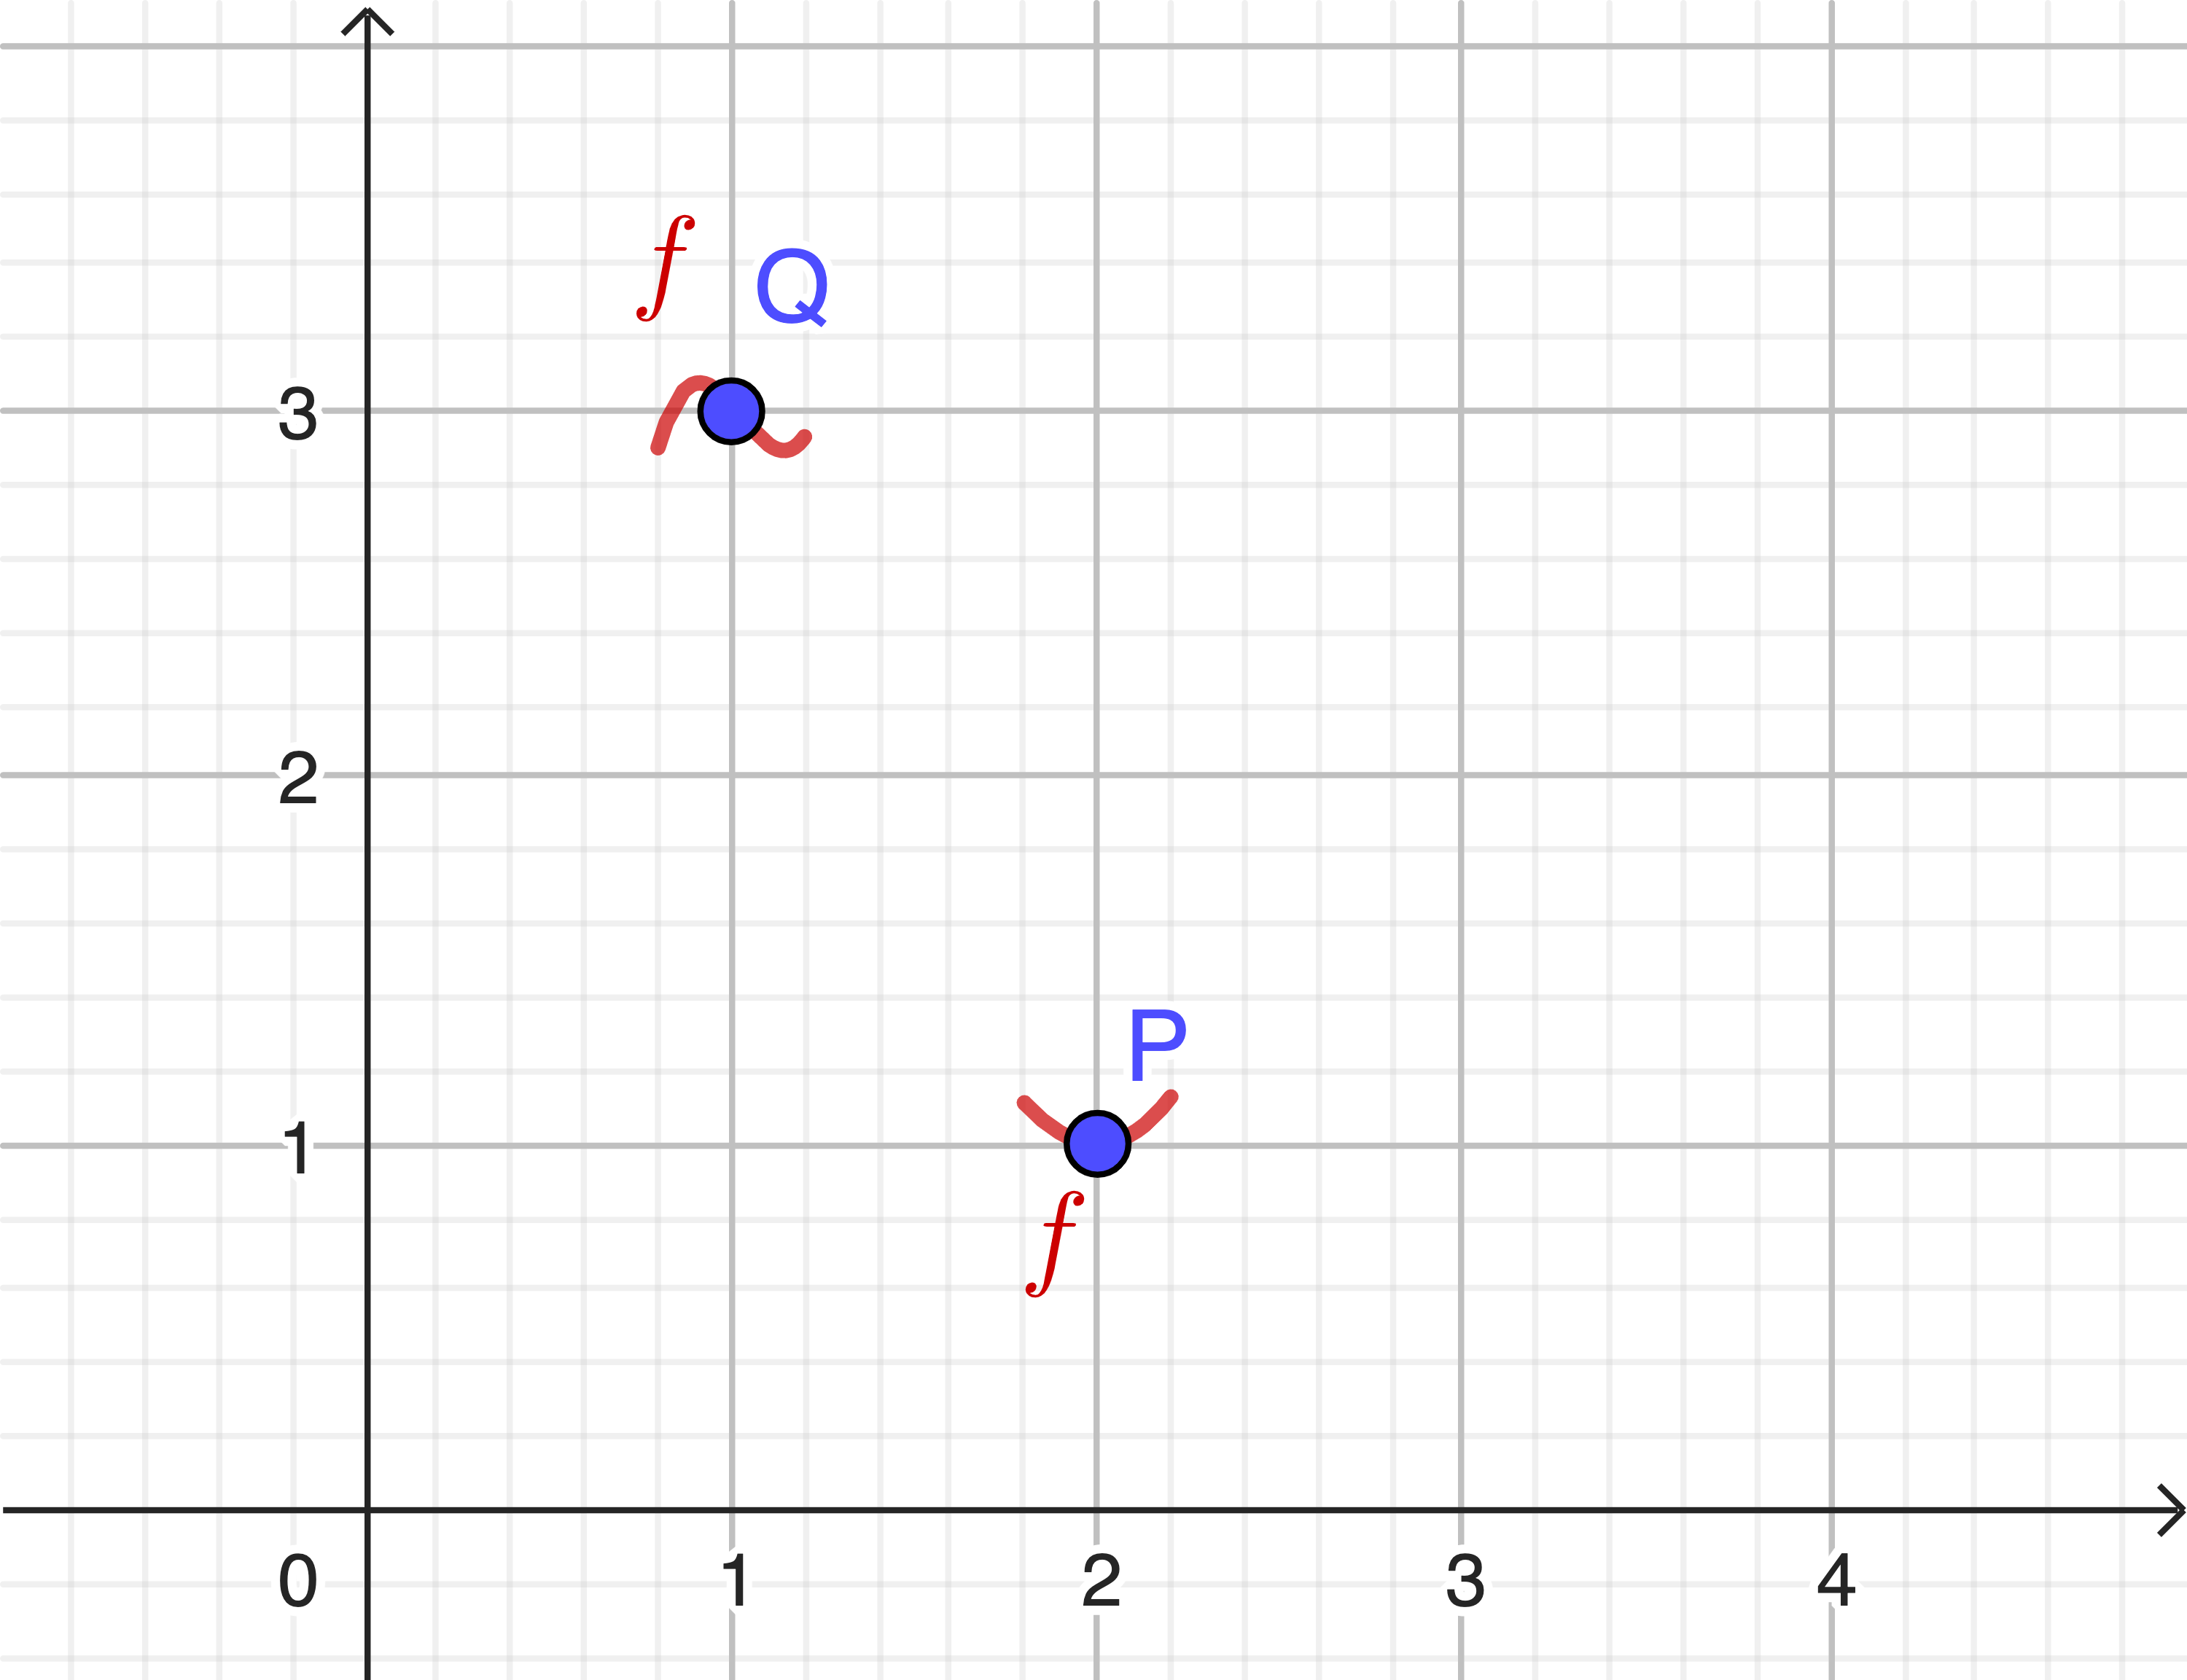
\includegraphics[scale=0.8]{media/fuBest.png}
	\end{center}

	\vspace*{11cm}


	\pagebreak

	\phantom{hello}

	\vspace*{19 cm}

\end{bsp}

\clearpage
\begin{ueb}{}{}
	\begin{enumerate}
		\item Der Graph einer Polynomfunktion 3. Grades hat im Punkt \( P(2,1) \) einen Terrassenpunkt und schneidet die \( x \)-Achse im Punkt \( A(4,0) \). Bestimmen Sie die Funktionsgleichung.
		\item Der Graph einer Polynomfunktion 4. Grades berührt die \( x \)-Achse bei \( x = 0 \). Im Punkt \( T(3,9) \) ist ein Terrassenpunkt. Bestimmen Sie die Funktionsgleichung.
		\item Der Graph einer Polynomfunktion 3. Grades hat einen Wendepunkt bei \( W(1,2) \) und berührt die \( x \)-Achse bei \( x = 2 \). Bestimmen Sie die Funktionsgleichung.
		\item Bestimmen Sie eine Polynomfunktion 3. Grades mit einer Nullstelle bei \( x = -2 \). Der Punkt \( P(0,y_P) \) ist ein Wendepunkt und die Wendetangente \( t \) hat die Gleichung \( y = \frac{1}{3}x +2 \).
		\item Wie lautet die Gleichung der Polynomfunktion 5. Grades, deren zum Ursprung punktsymmetrischer Graph in \( P(1,8) \) einen Terrassenpunkt hat?
		\item Eine zum Ursprung punktsymmetrische Polynomfunktion 3. Grades hat im Punkt \( M(3,-6) \) ein Minimum. Bestimmen Sie die Funktionsgleichung.
		\item Bestimmen Sie \( a \) so, dass der Graph der Funktion \( f \) mit
		      \[
			      f(x) = \frac{1}{2}(x^4 - ax^2)
		      \]
		      bei \( x = 1 \) einen Wendepunkt hat. Wo liegt der andere Wendepunkt? Bestimmen Sie auch noch die Extrema.

		      % \item Eine Polynomfunktion \( f \) hat an der Stelle \( x = 1 \) eine doppelte Nullstelle und es ist \( f''(x) = 6x \). Bestimme die Gleichung dieser Polynomfunktion und zeichne ihren Graphen.

		      % \item Bestimme die Gleichung einer Funktion \( f \) mit einem lokalen Maximum im Punkt \( (1\,|\,1) \) und einem lokalen Minimum im Punkt \( (-1\,|\,-1) \).

		\item  Bestimmen Sie die Gleichung von \( f \), wenn der Übergang vom Parabelbogen zur Strecke \( s \) an der Stelle \( (2, 0) \) knickfrei ist.
		      \begin{center}
			      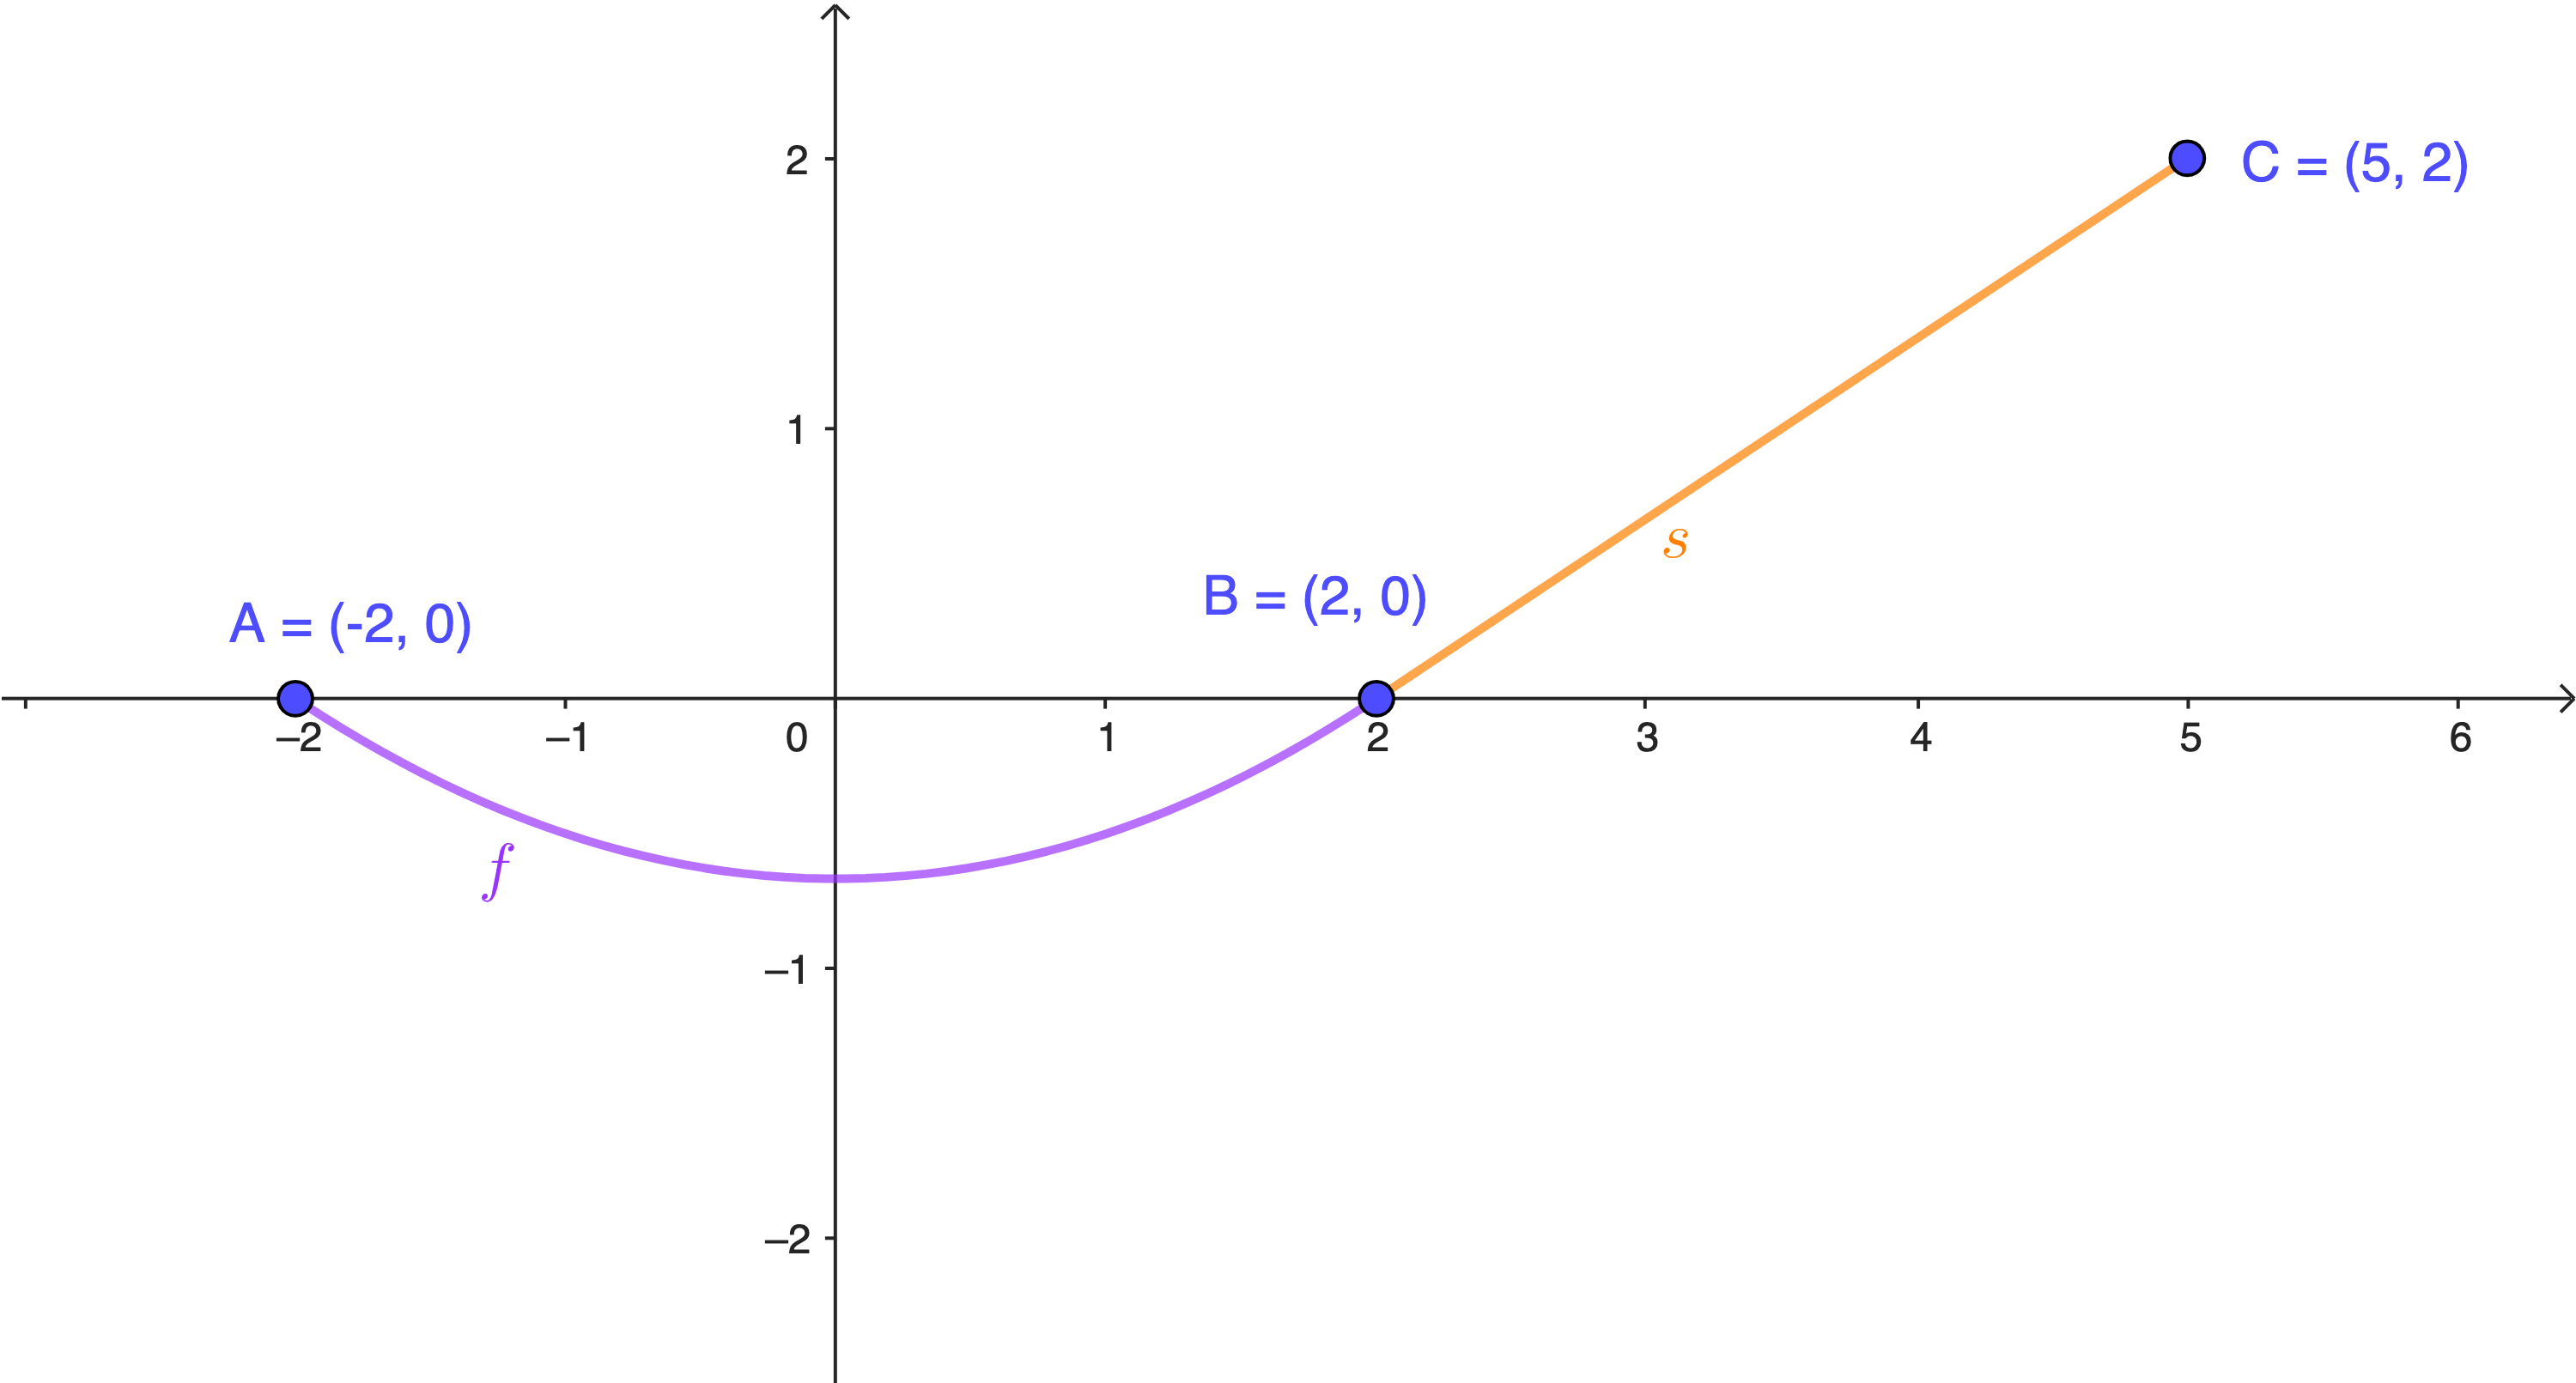
\includegraphics[width = 0.6 \textwidth]{media/knickfrei.png}
		      \end{center}

		\item Gegeben sind die geradlinigen Strassenabschnitte \( u = P(-3, 2)Q(-1, 0) \) und \( w = R(1, 0)S(5, 2) \).\\
		      Es soll eine krummlinige Verbindungsstrasse \( v \) von \( Q \) nach \( R \) gebaut werden, und zwar so, dass die Übergänge in \( Q \) und \( R \) \emph{knickfrei} werden. Beschreiben Sie den Strassenverlauf von \( v \) mit einer Polynomfunktion 3. Grades, die diese Eigenschaft an den beiden Übergangsstellen \( Q \) und \( R \) in die daran anschliessenden geradlinigen Strassenabschnitte nach \( P \) respektive \( S \) besitzt.
	\end{enumerate}

\end{ueb}

\clearpage
\emph{Lösungen:}
\begin{enumerate}
	\item \( f(x) = -\frac{1}{8}x^3 + \frac{3}{4}x^2 - \frac{3}{2}x + 2 \)
	\item \( f(x) = \frac{1}{3}x^4 - \frac{8}{3}x^3 + 6x^2 \)
	\item \( f(x) = x^3 - 3x^2 + 4 \)
	\item \( f(x) = \frac{1}{6}x^3 + \frac{1}{3}x + 2 \)
	\item \( f(x) = 3x^5 - 10x^3 + 15x \)
	\item \( f(x) = \frac{1}{9}x^3 - 3x \)
	\item $a=6, W_2 =(-1, -2.5), H=(0,0), T_{1,2} = \left(\pm\sqrt{3}, -\frac{9}{2}\right)$
	\item $f(x) = \frac{1}{6} x^2 - \frac{2}{3}$
	\item $v(x) = \frac{1}{8}\left(-x^3+3x^2+x-3\right)$ Wenn man es geschickt anstellt, ist das Gleichungssystem nicht so schwer \dots
\end{enumerate}

\clearpage
\begin{ueb}
	{Modellierung der Bewegung eines Roboterarms}{}
	Um einen Roboterarm eine gewünschte Bewegung ausführen zu lassen, muss die Geschwindigkeit der Drehachse von 0 Umdrehungen pro Sekunde (U/sec) auf 10 U/sec erhöht werden. Dies muss innerhalb von 4 Sekunden geschehen. Die Geschwindigkeit $v$ ist somit eine Funktion der Zeit $t$. Damit der Roboter bei der Ausführung dieser Operation keinen Schaden erleidet, werden gewisse Anforderungen an diese Funktion gestellt: Die Geschwindigkeit soll sich nicht sprunghaft ändern, und auch die Beschleunigung darf keine Sprünge machen. Am Anfang ist die Beschleunigung 0 U/sec\textsuperscript{2}, und am Schluss soll sie auch wieder 0 U/sec\textsuperscript{2} betragen.

	Dies lässt sich erreichen, indem eine Geschwindigkeitsfunktion der Form
	\[v(t)=at^3+bt^2+ct+d\]
	gewählt wird, um die Bewegung des Roboters zu steuern.
	\begin{enumerate}
		\item Berechnen Sie die Koeffizienten $a,b,c,d$.
		\item Zu welchem Zeitpunkt ist die Beschleunigung maximal? Wie gross sind zu diesem Zeitpunkt die Geschwindigkeit und die Beschleunigung?
		\item Erstellen Sie ein zweites Geschwindigkeitsprofil. Wählen Sie von
		      (0,0) nach (2,6) ein Parabelstück mit dem Scheitelpunkt in (0,0) und ein weiteres Parabelstück von (2,6) bis (4,10) mit Scheitelpunkt in (4,10). Erfüllt Ihr Geschwindigkeitsprofil die gestellten Bedingungen?
	\end{enumerate}

	% \vspace{
	%     10cm
	% }



\end{ueb}
\pagebreak
Lösungen der Aufgabe \glqq Roboterarm\grqq{}
\begin{enumerate}
	\item 	Das Gleichungssystem:
	      \begin{align*}
		      v(0)  & = 0  \\
		      v(4)  & = 10 \\
		      v'(0) & = 0  \\
		      v'(4) & = 0
	      \end{align*}
	      liefert die Lösung $a=-\frac{5}{16}, b=\frac{15}{8}, c=d=0$. Die Funktion lautet also $v(t)=-\frac{5}{16}t^3 +  \frac{15}{8} t^2 $
	\item Die Beschleunigung ist dort maximal, wo die Geschwindigkeit am stärksten ansteigt, also beim Wendepunkt. Die Gleichung $v''(t)=0$ liefert die Lösung $t=2$. Zu diesem Zeitpunkt ist $v(2)=5$ U/sec und $v'(2)=\frac{15}{4}$ U/sec\textsuperscript{2}.
	\item Die Funktion $v_1$ hätte dann die Gleichung $v_1 (t)=\frac{3}{2}t^2$ (mit einem Gleichungssystem). Die Funktion $v_2$ die Gleichung $v_2 (t)=-t^2+8t-6$.
	      Diese Kombination aus zwei Parabeln erfüllt die Bedingungen nicht, weil sich die Beschleunigung bei $t=2$ \glqq ruckartig\grqq{} ändern würde, womit sie nicht stetig wäre. Es gilt nämlich $v_1'(2)=6\neq 4 = v_2' (t)$

\end{enumerate}

\clearpage
\begin{ueb}
	{Aufgaben mit weiteren Funktionstypen}{}
	\begin{enumerate}
		\item Bestimmen Sie die Parameter $a$ und $b$, sodass die Funktion stetig und knickfrei ist.
		      \begin{enumerate}
			      \item $f(x) = \begin{cases}
					            (x^2-2)^3      & x \le 1 \\
					            \frac{ax+b}{x} & x > 1
				            \end{cases}$
			      \item $f(x) = \begin{cases}
					            \frac{x+a}{ax}  & x \le -1 \\
					            \frac{bx}{x+2a} & x > -1
				            \end{cases}$
			      \item $f(x) = \begin{cases}
					            \sqrt{4x-3}     & x > 1   \\
					            \frac{ax}{bx+2} & x \le 1
				            \end{cases}$
			      \item $f(x) = \begin{cases}
					            a\cdot \sin(x)      & x \le \frac{\pi}{6} \\
					            6\cdot \cos(2x) + b & x > \frac{\pi}{6}
				            \end{cases}$
		      \end{enumerate}

		\item Der Graph der Funktion $f\colon y=\frac{p x}{x-2}$ hat bei $x=4$ die Steigung $m=5$. Berechnen Sie den Wert von $p$.
		\item Bestimmen Sie $a$ und $b$ so, dass der Graph von $f\colon y=\frac{a x^{2}+1}{b x}$ in $P(2,1)$ ein Extremum besitzt. (Tipp: Wenn Sie zuerst den Funktionsterm ausdividieren, ist die Ableitung einfacher zu berechnen.)
		\item Der Graph der Funktion $f\colon y=\frac{a x^{2}+b}{x-3}$ besitzt in $P(-1, 4)$ die Steigung $m=-3$. Bestimmen Sie $a$ und $b$ sowie die Gleichung der Tangente in $P$.
		\item Bei $x=4$ besitzt der Graph der Funktion $f\colon y=x\sqrt{a-x}$ ein Extremum. Berechnen Sie den Wert von $a$.
		\item Bestimmen Sie $a$ und $b$ so, dass die Kurve $f\colon y=a x+\sqrt{x+b}$ in $P(3, 10)$ die Steigung $m=7/2$ hat. (Tipp: Beim Gleichungssystem kann man die Unbekannte $b$ eliminierten, indem man $\sqrt{3+b}$ aus der einen Gleichung isoliert und in die andere einsetzt.)
		\item Der Graph der Funktion $f\colon y=a\cdot \sin x + 2x$ besitzt bei $x=\frac{\pi}{3}$ ein Extremum. Berechnen Sie den Wert von $a$.
		\item Bestimmen Sie $a$ so, dass der Graph der Funktion $f\colon y=\cos^{2}x + a\cdot \sin x$ bei $x=\frac{\pi}{4}$ eine Tangente mit der Steigung $m=1$ besitzt.
		      % \item Die Graphen von $f_{1}\colon y=a\cdot \tan x + b$ und $f_{2}\colon y=\sqrt{2}\cdot \sin 3x + 2a$ berühren sich bei $x=\frac{\pi}{4}$.
		      %       \begin{enumerate}
		      % 	      \item Bestimmen Sie $a$ und $b$.
		      % 	      \item Welche Gleichung hat die gemeinsame Tangente bei $x=\frac{\pi}{4}$?
		      %       \end{enumerate}
		      % \item Der Graph der Funktion $f\colon y=\frac{x^{3}-5x+a}{4x^{3}}$ hat bei $x=3$ eine Nullstelle. Ermitteln Sie $a$ und zeigen Sie, dass es keine weiteren Nullstellen gibt.
		\item Für welchen Wert von $a$ und $b$ berührt die Kurve $f\colon y=(x+a)\sqrt{b x}$ bei $x=1$ die Gerade durch $P(4, 1)$ und $Q(-2, -5)$?
		\item Für welchen Wert von $a>0$ schneiden sich die Gerade $g\colon y=a x$ und die Kurve $f\colon y=\sqrt{2-ax}$ in einem rechten Winkel?


		      % Zur Exponentialfunktion:

		\item Berechnen Sie $a$ und $b$ so, dass der Graph der Funktion
		      \[
			      f\colon y=(x^{2}+b)\cdot e^{a x}
		      \]
		      in der Nullstelle $N(3,0)$ die Steigung $m=6 e$ hat.

		\item Die Kurve
		      \[
			      f\colon y=a x^{2}\cdot e^{b x}
		      \]
		      hat bei $x=1$ ein Extremum und bei $x=-\frac{1}{2}$ die Steigung $m=-\frac{3}{2} e$. Bestimmen Sie $a$ und $b$.

		\item Der Graph der Funktion
		      \[
			      f\colon y=(a x+1)\cdot e^{-x}
		      \]
		      hat bei $x=0$ ein Extremum. Berechnen Sie $a$, entscheiden Sie, ob es sich um ein Minimum oder Maximum handelt und berechnen Sie die Koordinaten des Wendepunktes.


	\end{enumerate}
\end{ueb}
\clearpage
\emph{Lösungen}
\begin{enumerate}
	\item Knickfreie, stetige Funktionen
	      \begin{enumerate}
		      \item $a=5, b=-6$
		      \item $a=3/4, b= -1/6$
		      \item $a=1, b=-1$
		      \item $a=-12, b= -9$
	      \end{enumerate}
	\item $p=-10$
	\item $a=1/4, b=1$
	\item $a=b=-8, t(x)=-3x+1$
	\item $a=6$
	\item $a=3, b=-2$
	\item $a=-4$
	\item $a=2\sqrt{2}$
	      % \item $a=-1.5, b = -0.5, t(x)=-3x + \frac{3\pi-8}{4}$
	      % \item $a=-12$
	\item $a=-2, b=4$
	\item $a= \sqrt{2}$

	      % Zur Exponentialfunktion:
	\item $a=1/3, b=-9$
	\item $a=1, b= -2$
	\item $a=1$ Es ist ein Hochpunkt. Der Wendepunkt liegt bei $W(1, 2/e)$.

\end{enumerate}
\clearpage
\subsection{Extremwerprobleme}
\begin{LA}
	{Einführungsaufgabe}{}
	\begin{enumerate}


		\item Zwischen 08:00 Uhr und 18:00 Uhr wird in der Mensa der KS Im Lee die Lufttemperatur gemessen. Die Messungen wurden in das Koordinatensystem unten eingetragen. Wann ungefähr ist die Temperatur am höchsten? Wann am tiefsten?
		      \begin{center}
			      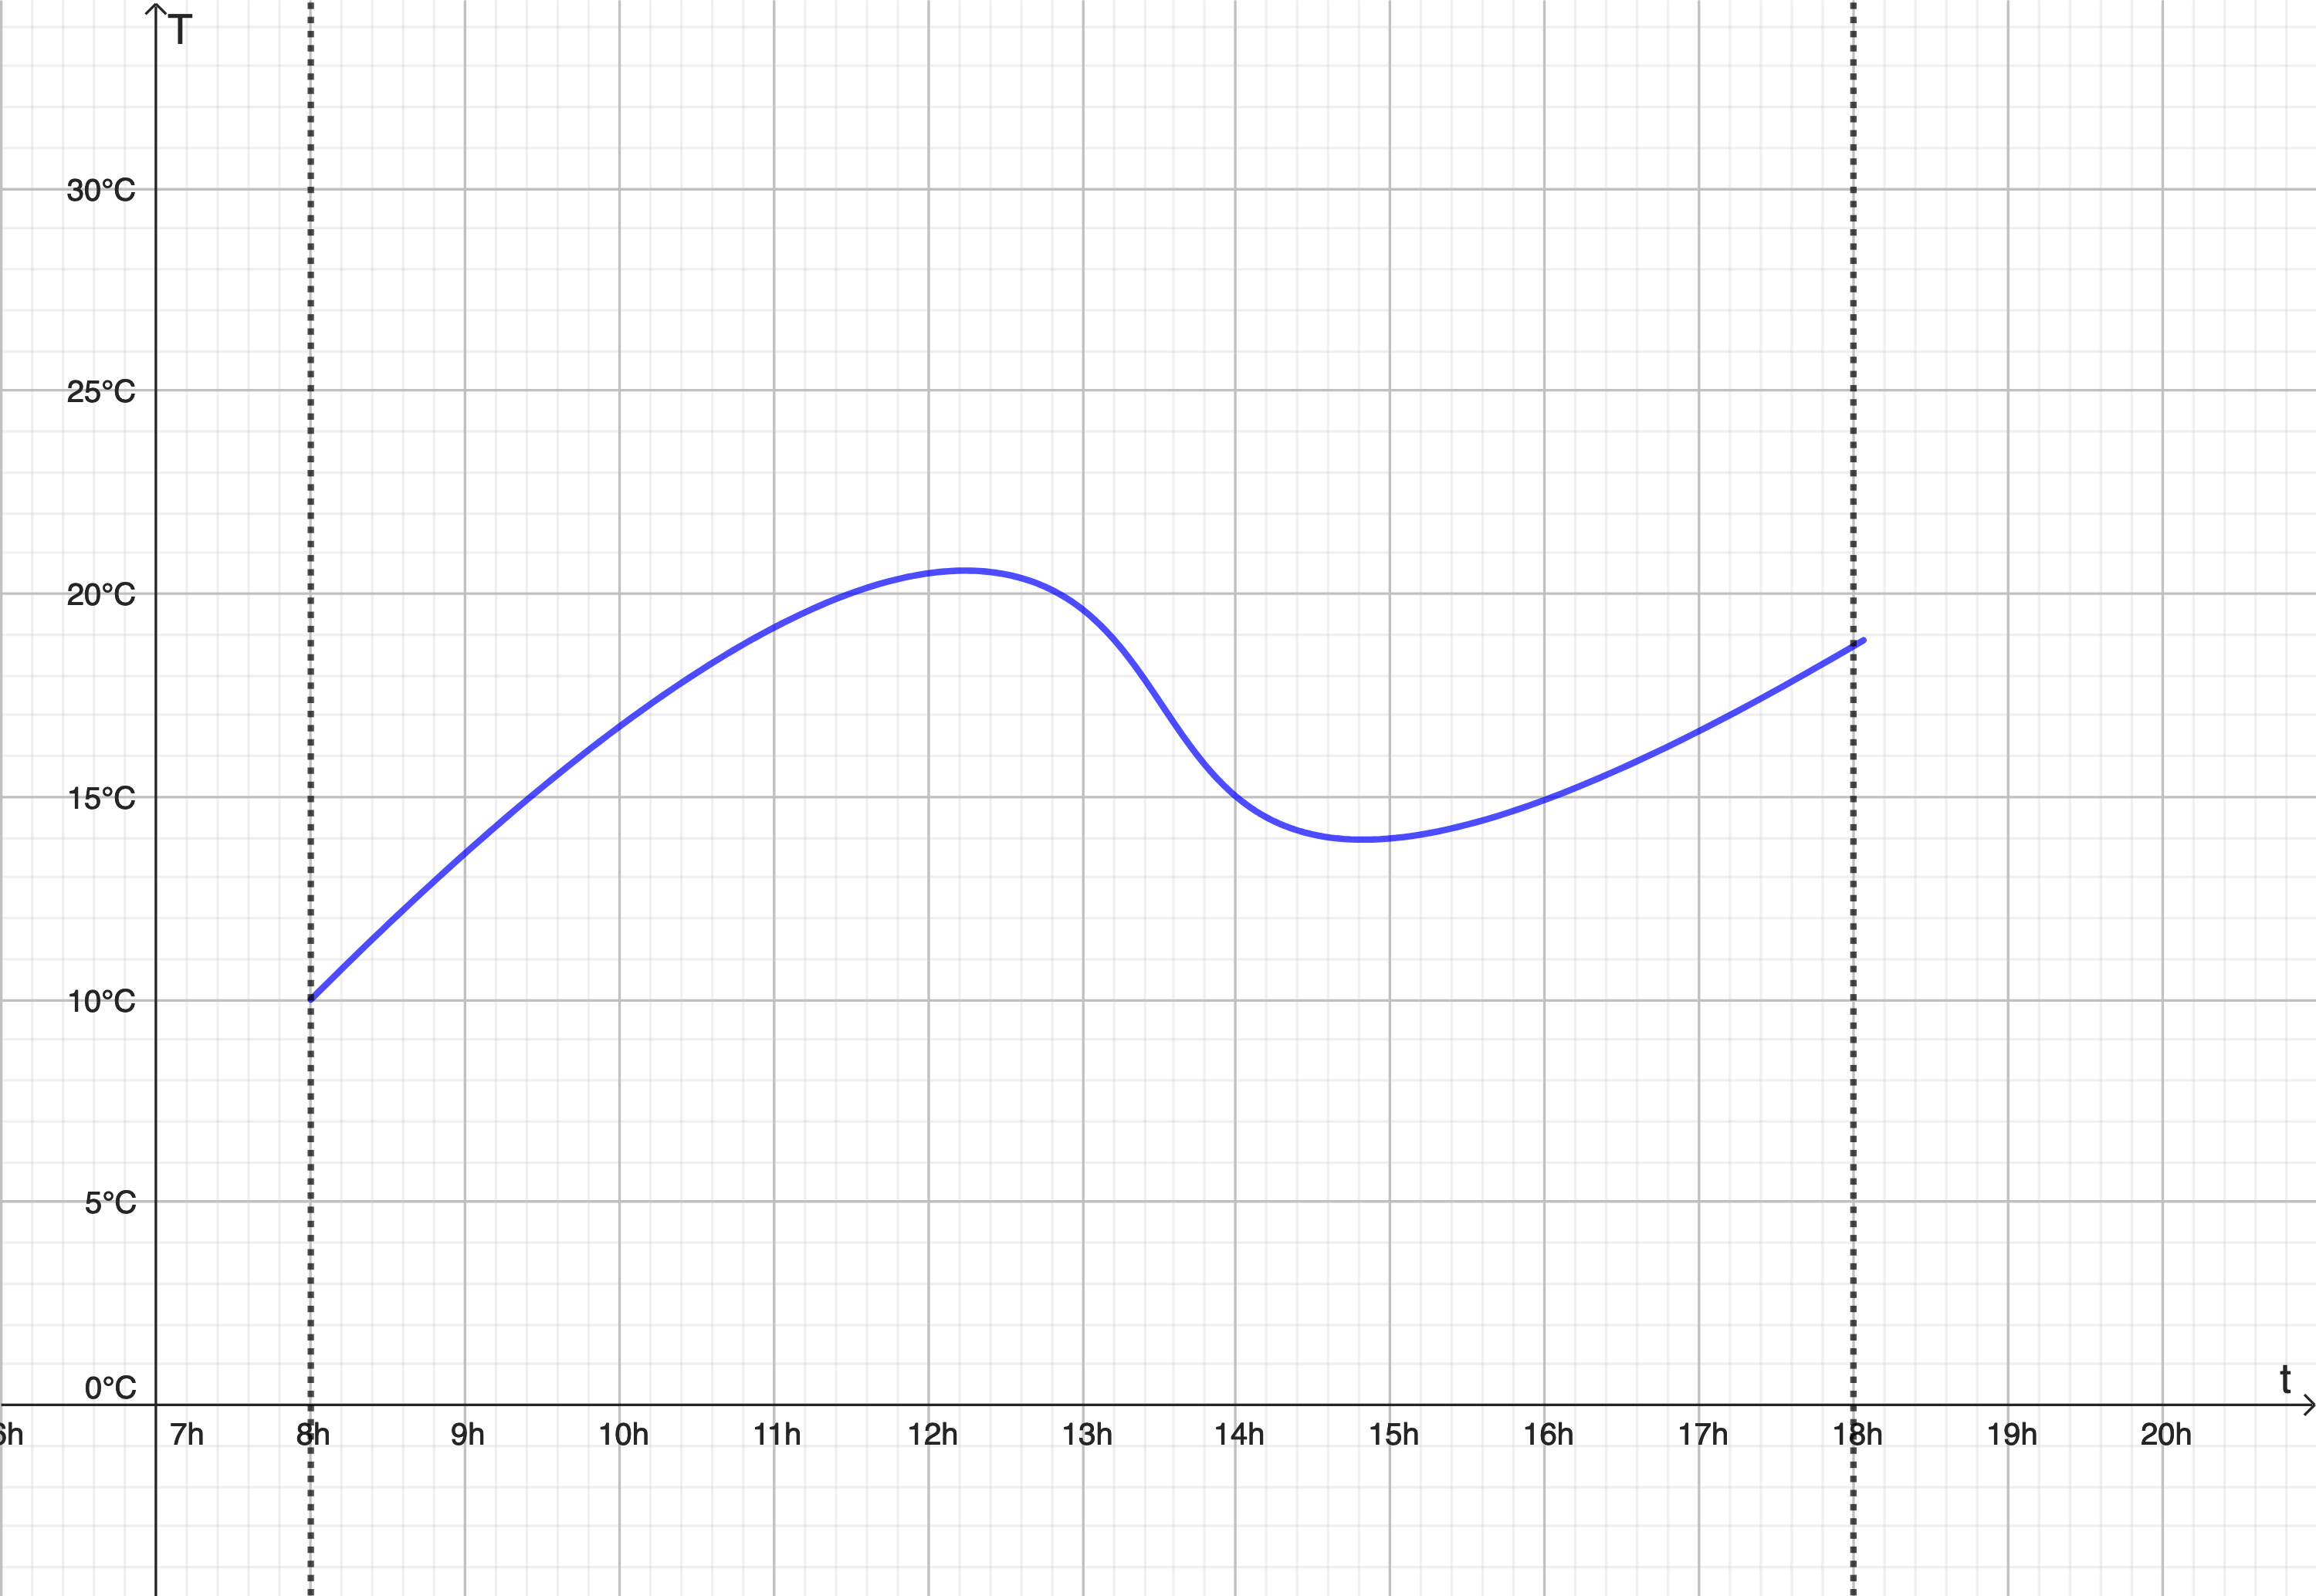
\includegraphics[width=0.9\textwidth]{media/globalMaxEaufgabe.png}
		      \end{center}

		\item Eine Flüssigkeit wird im Rahmen eines Experiments zuerst etwas aufgewärmt, dann in die Kälte gestellt. Der Temperaturverlauf während den ersten fünf Minuten des Experiments lässt sich durch die folgende Funktion modellieren: $T(t)=-t^2+4t+16$, für $t\in [0,5]$. Zu welchem Zeitpunkt in diesen ersten fünf Minuten war die Temperatur am höchsten? Wann am niedrigsten? (Es könnte hilfreich sein, den Graphen zu skizzieren).

		\item Bestimmen Sie den höchsten und niedrigsten Wert der Funktion $f(x)=x^3-3x$ im Intervall $x\in[-4, \frac{3}{2}]$.

		\item Gesucht ist der höchste Wert einer Funktion $f(x)$ im Intervall $x\in [a,b]$. Beschreiben Sie, wie man vorgehen soll, um die Aufgabe zu lösen. Welche Gleichungen muss man lösen? Welche Werte kommen infrage?
	\end{enumerate}

\end{LA}
\clearpage
\begin{definition}
	{Globale Extrema}{}
	Sei $f$ eine auf dem Intervall $[a,b]$ definierte, differenzierbare Funktion. Eine Stelle $x_0 \in [a,b]$ heisst \emph{globales Maximum} (bzw.\ \emph{Minimum}) der Funktion $f$ im Intervall $[a,b]$, falls für alle $x \in [a,b]$ gilt: $f(x) \le f(x_0)$ (bzw.\ $f(x)\ge f(x_0 )$).
\end{definition}

Betrachten Sie den folgenden Graphen einer Funktion im Intervall $[a,b]$

\begin{center}
	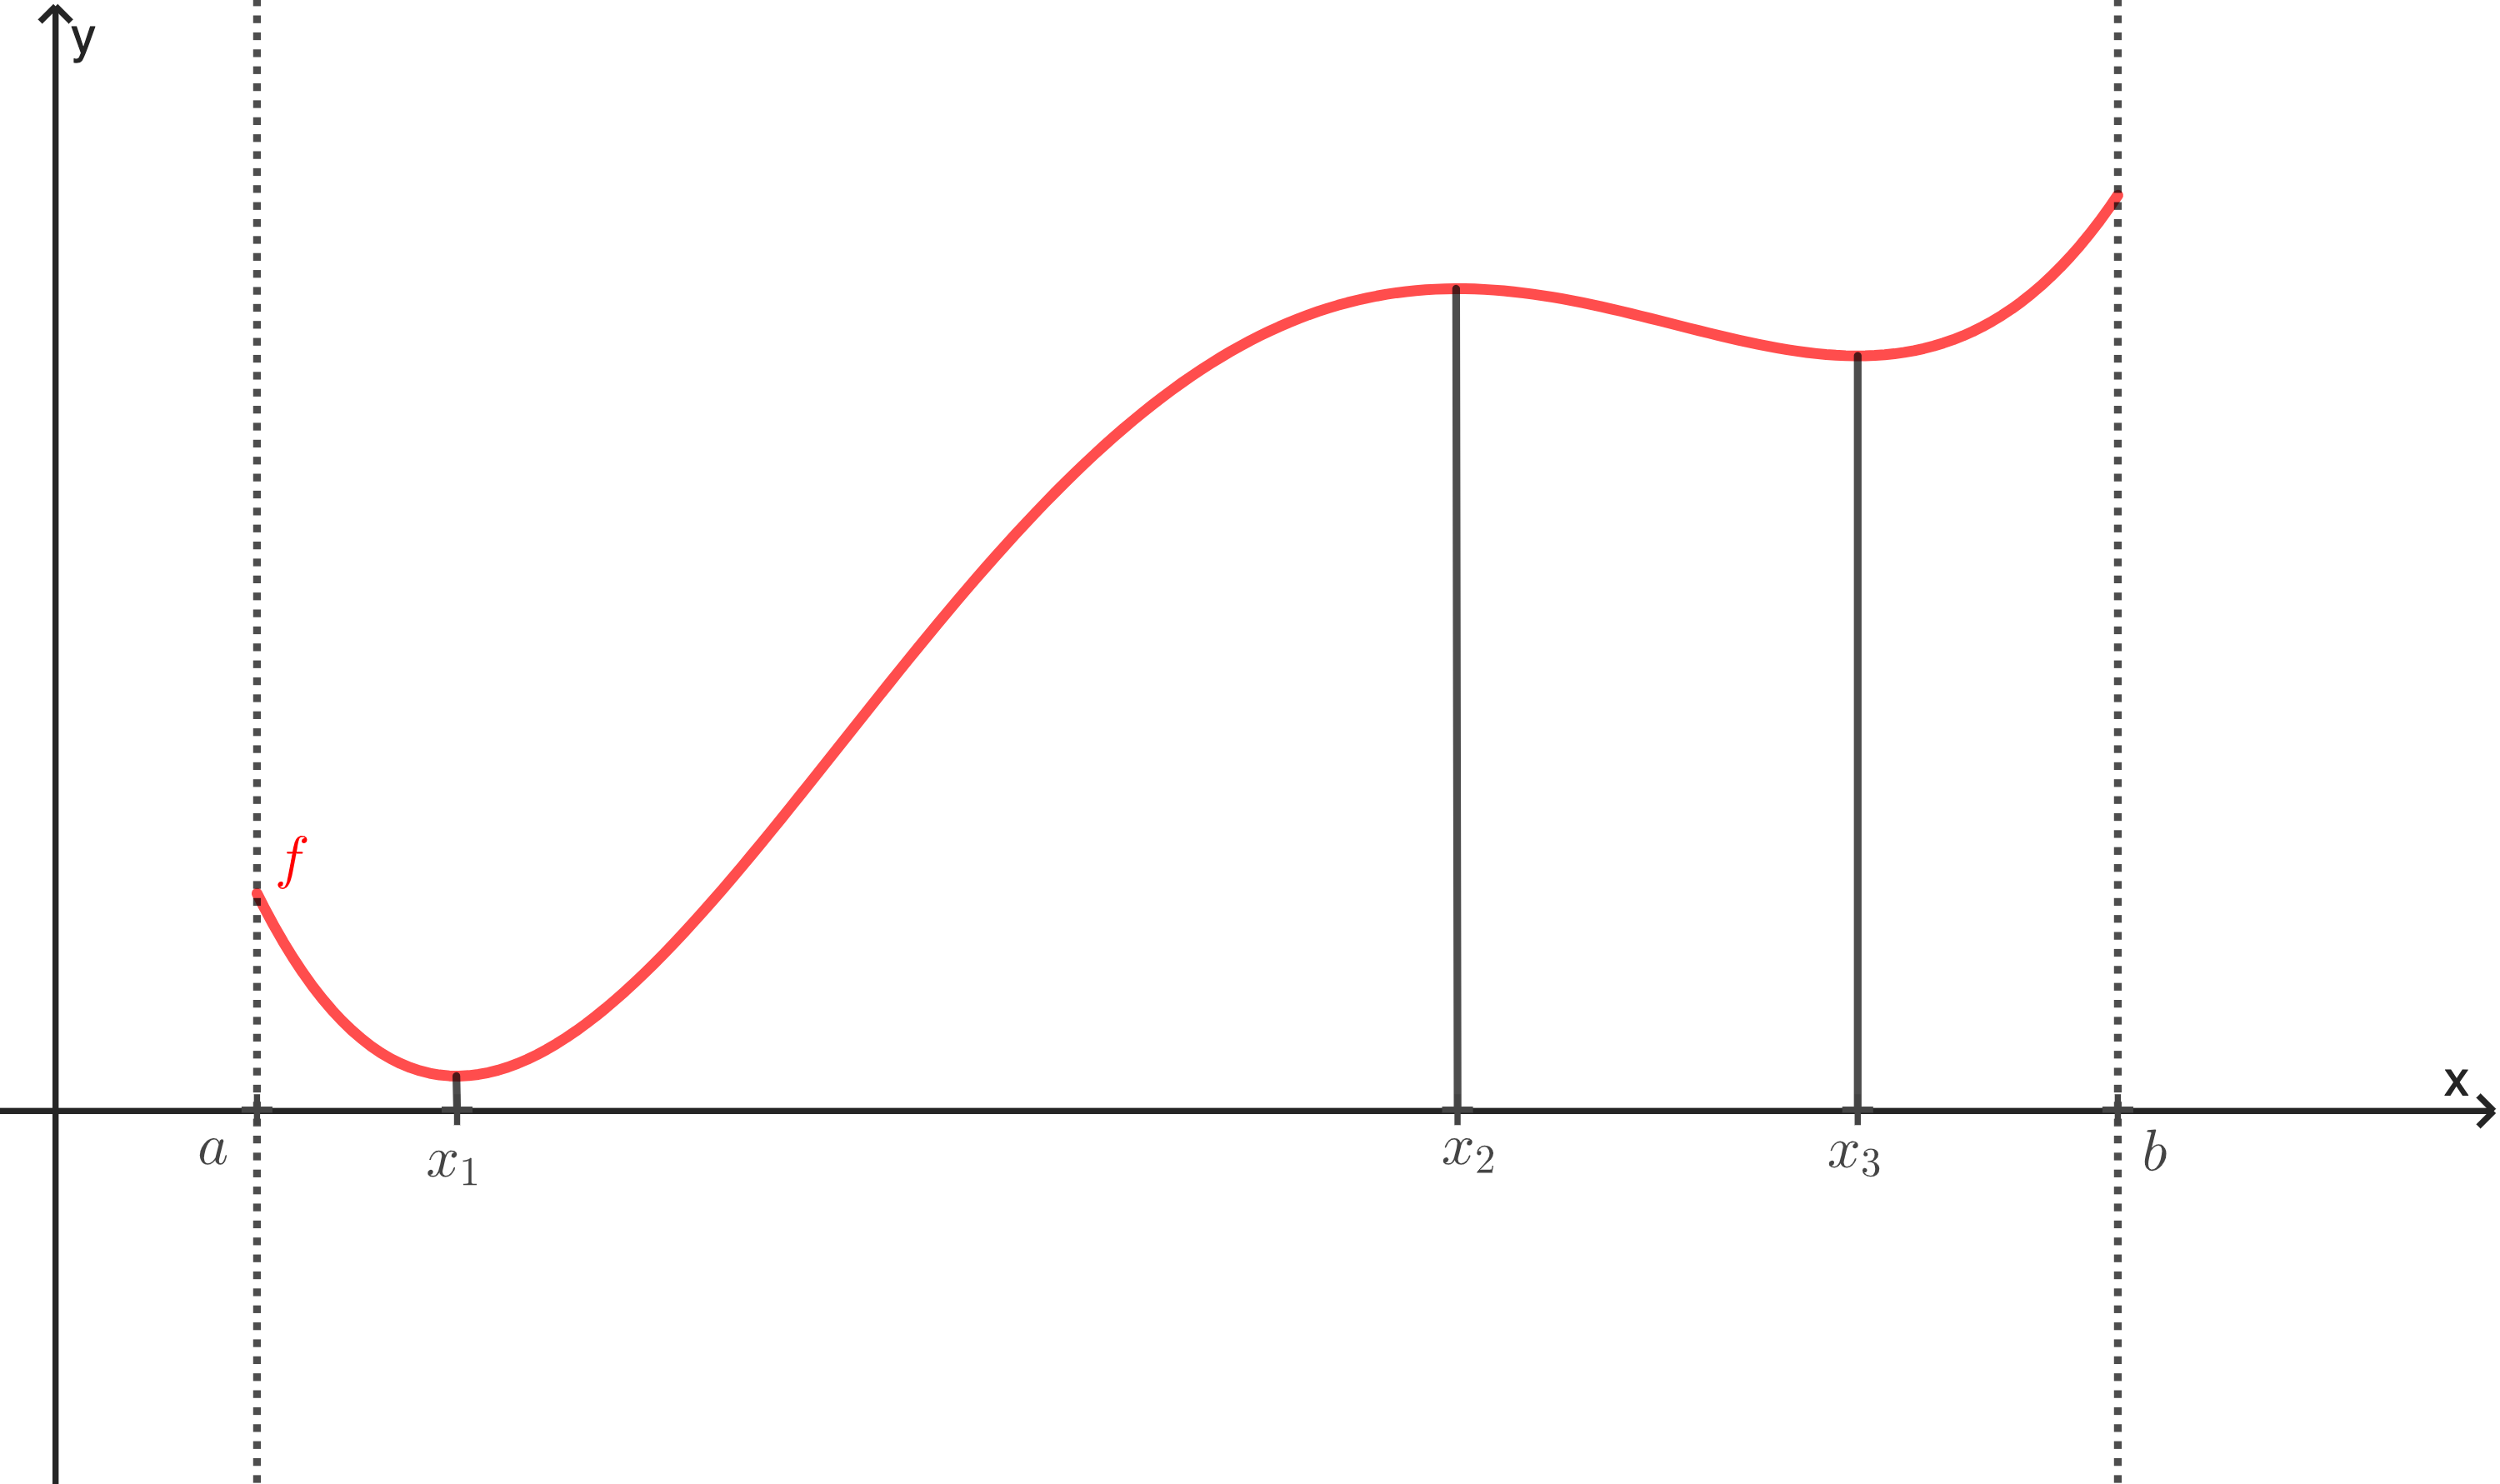
\includegraphics[width=0.6\textwidth]{media/globalExtremaDef.png}
\end{center}

Die Funktion hat die \textbf{lokalen} Extremalstellen $x_1,x_2$ und $x_3$.\\
Das \textbf{globale} Minimum ist an der Stelle $x_1$.\\
Das \textbf{globale} Maximum ist an der Stelle $b$.

Bei Anwendung sind oft die globalen Extremalstellen einer Funktion gesucht. Die Kosten wollen minimiert werden, der Ertrag will maximiert werden, usw.

Zum Auffinden der globalen Extremalstellen einer Funktion $f$ im Intervall $[a,b]$ kann man wie folgt vorgehen:
\begin{enumerate}
	\item Finde alle Stellen $x_1,x_2,\ldots ,x_n$ mit $f' (x)=0$ (Nullstellen der Ableitung).
	\item Die Kandidaten für das globale Extremum sind $x_1,x_2,\ldots ,x_n,a$ und $b$.
	\item Vergleiche die Werte $f(x_1 ),f(x_2 ),\ldots ,f(x_n ),f(a)$ und $f(b)$.
\end{enumerate}

\begin{bsp}
	{Globales Maximum der Funktion $f(x)=x^3-3x$ im Intervall $x\in [-4, \frac{3}{2}]$.}{}
	\begin{enumerate}
		\item $f'(x)=3x^2-3 \stackrel{!}{=} 0 \iff x_{1,2}=\pm 1$.
		\item Kandidaten: $x_1=-1,x_2=1,a=-4,b=\frac{3}{2}$.
		\item Vergleich:
		      \begin{center}
			      \begin{tabular}{c|| c|c|c|c}
				      $x$    & $-4$  & $- 1$ & $1$  & $\frac{3}{2}$ \\ \hline
				      $f(x)$ & $-52$ & $2$   & $-2$ & $-1.125$
			      \end{tabular}
		      \end{center}

		      Das globale Maximum im Intervall $x\in [-4,3/2]$ wird an der Stelle $x=-1$ erreicht, das globale Minimum an der Stelle $x=-4$.
	\end{enumerate}
\end{bsp}

\begin{bsp}
	{Musteraufgabe: Die beste Schachtel}{}
	Von einer A4-Seite ($21 \times 29$ cm) werden an den Ecken Quadrate mit der Seitenlänge $x$ cm abgeschnitten. Wie ist $x$ zu wählen, damit der Rest durch Falten eine Schachtel (ohne Deckel) mit maximalem Inhalt ergibt?

	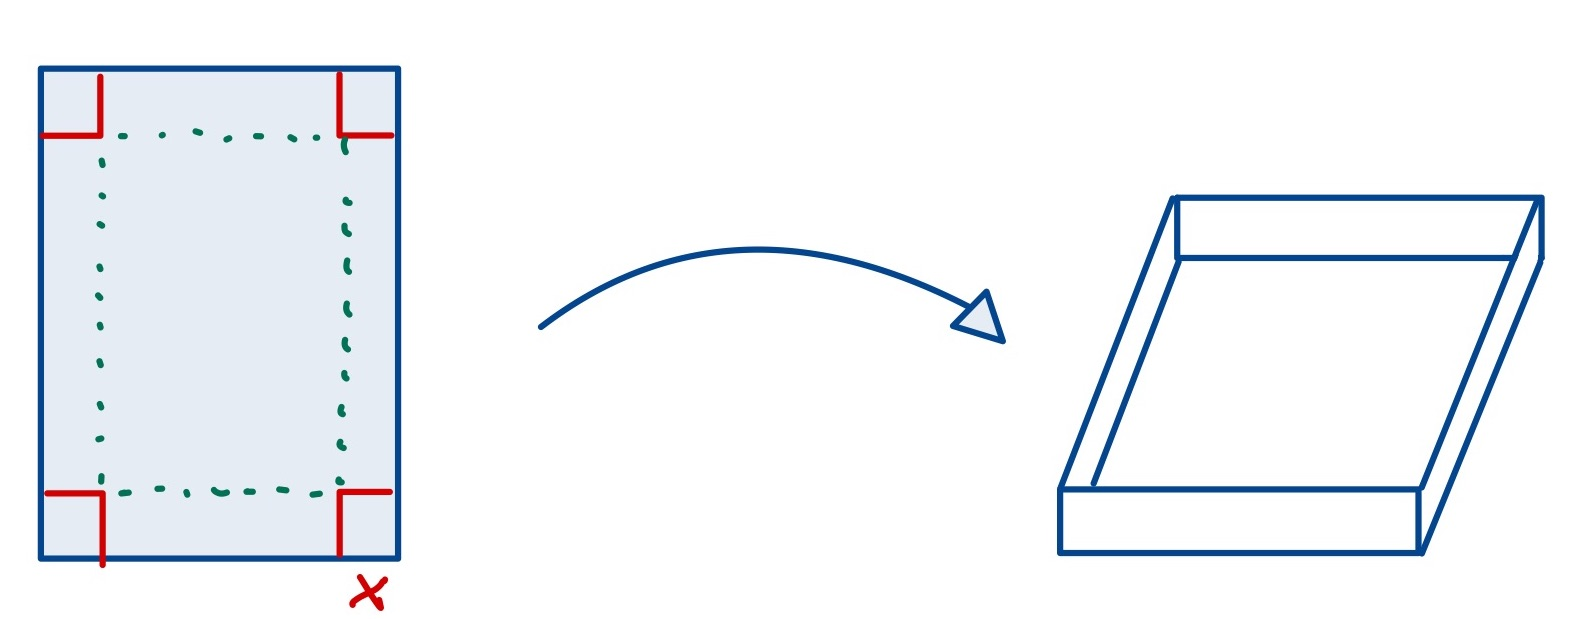
\includegraphics[width = 0.4\textwidth]{media/besteSchachtel.jpg}

	\vspace{14cm}
\end{bsp}

\pagebreak


\pagebreak
\begin{bsp}
	{Musteraufgabe: Ersatzfunktion}{Ersatzfunktion}
	Welcher Punkt der Parabel $y=x^2$ liegt am nächsten zum Punkt $A=(0,1)$?
	\vspace*{19cm}

	% \tcbvfill
\end{bsp}
\pagebreak
\begin{ueb}
	{Extremalprobleme}{}
	\begin{enumerate}
		\item Der Karton ist 40\,cm lang und 25\,cm breit. Es soll eine Schachtel mit Deckel entstehen. Wie lang sind die Kanten der Schachtel mit maximalem Inhalt?
		      \begin{center}
			      \begin{tikzpicture}[scale=0.12]
				      %% Dunkle Felder oben
				      \fill[gray!60] (0,20) rectangle (10,30);
				      \fill[gray!60] (35,20) rectangle (45,30);

				      %% Dunkle Felder unten
				      \fill[gray!60] (0,-5) rectangle (10,5);
				      \fill[gray!60] (35,-5) rectangle (45,5);

				      %% Dunkle Felder rechts (vertikale Doppelzone)
				      \fill[gray!60] (45,-5) rectangle (70,5);
				      \fill[gray!60] (45,20) rectangle (70,30);

				      %% Linienraster
				      \draw[thick] (0,-5) rectangle (70,30);
				      \draw[dashed] (10,-5) -- (10,30);
				      \draw[dashed] (35,-5) -- (35,30);
				      \draw[dashed]  (45,-5) -- (45,30);
				      \draw[dashed]  (0,5) -- (70,5);
				      \draw[dashed]  (0,20) -- (70,20);

			      \end{tikzpicture}
		      \end{center}
		\item Das Kantenmodell eines Quaders, der dreimal so lang wie breit ist, wird aus 520\,cm Draht hergestellt. Wie sind die Kanten zu wählen, wenn die Oberfläche des Quaders möglichst gross sein soll?
		      % \item Ein Kreissektor von gegebenem Umfang \(u\) soll maximalen Flächeninhalt haben. Bestimmen Sie den Radius und den Zentriwinkel des Sektors.
		\item Eine Blechbüchse soll so hergestellt werden, dass sie ein Volumen von 1 Liter hat. Wie sind die Abmessungen der Büchse zu wählen, damit sie möglichst wenig Material verbraucht?
		      % , wenn sie
		      %       \begin{enumerate}
		      % 	      \item einen Deckel und einen Boden hat?
		      % 	      \item keinen Deckel hat?
		      %       \end{enumerate}
		\item Wie hoch ist der gerade Kreiskegel mit gegebener Mantellinie \(s\), der grösstmögliches Volumen besitzt? Tipp: Sie können wählen, ob Sie die Höhe oder den Grundkreisradius als Variable verwenden wollen. Je nach Wahl der Variable kann die Zielfunktion einfacher oder kompliziert sein. Wählen Sie weise!
		\item Einem geraden Kreiskegel (Grundkreisradius \(3\,\text{cm}\), Höhe \(6\,\text{cm}\)) ist der Kreiszylinder mit maximalem Volumen einzubeschreiben, der die gleiche Rotationsachse wie der Kegel hat. Bestimmen Sie die Zylinderhöhe.
		      \newcounter{temp}
		      \setcounter{temp}{\value{enumi}}
	\end{enumerate}
\end{ueb}

\begin{ueb}
	{Noch mehr Extremalprobleme (nach \Cref{bsp:Ersatzfunktion})}{}
	\begin{enumerate}\setcounter{enumi}{\value{temp}}
		\item Welcher Punkt auf der Parabel \(p:\; y = 0.5x^{2}\) hat den kürzesten Abstand vom Punkt \(P(6, 0)\)? \\
		      Beim Lösen werden Sie vermutlich auf eine Gleichung dritten Grades stossen. Lösen Sie diese mit der Funktion poly-solv des Taschenrechners.
		\item
		      \begin{enumerate}
			      \item Skizzieren Sie die Parabel \(p:\; y = 5x - x^{2}\).
			      \item Der Punkt \(A(a, b)\) liegt im 1.\,Quadranten auf der Parabel \(p\). Bestimmen Sie die Koordinaten von \(A\) so, dass das Rechteck, von dem zwei Seiten auf den Koordinatenachsen liegen und von dem \(A\) eine Ecke ist, möglichst grossen Umfang hat.
		      \end{enumerate}
		\item Lösen Sie das gleiche Problem für die Parabel \(p:\; y = 3x - x^{2}\); diesmal soll das Rechteck maximalen Flächeninhalt haben.

		\item Die Parabel mit der Gleichung $y=\frac{1}{4}x^4+4$ und die zur $y$-Achse parallele Gerade an der Stelle $x=8$ begrenzen im 1. Quadranten ein Gebiet, in welches ein Rechteck mit grösstmöglichem Inhalt einbeschrieben werden soll. Die Seiten des Rechtecks sollen parallel zu den Koordinatenachsen verlaufen. Bestimmen Sie die Koordinaten der Ecke $P$ auf dem Parabelbogen.


		\item Dem Flächenstück, das die Parabel \(p:\; y = a - x^{2}\) \((a > 0)\) mit der \(x\)-Achse einschliesst, ist ein Rechteck so einzubeschreiben, dass es bei Rotation
		      \begin{enumerate}
			      \item um die \(y\)-Achse den Zylinder mit maximalem Volumen erzeugt;
			      \item um die \(x\)-Achse den Zylinder mit maximalem Volumen erzeugt. \\
			            Beim Lösen werden Sie vermutlich auf eine biquadratische Gleichung stossen. Lösen Sie diese mit einer Substitution der Form $t= u^2$ (Variablennamen entsprechend anpassen).
		      \end{enumerate}
		      Berechnen Sie die Seitenlängen dieses Rechtecks.
	\end{enumerate}


\end{ueb}

\pagebreak
\emph{Lösungen:}

\begin{enumerate}
	\item \(x = 5\,\text{cm}\), Schachtel: \(15 \times 15 \times 5\).
	\item Breite \(= 20\,\text{cm}\), Länge \(= 60\,\text{cm}\), Höhe \(= 50\,\text{cm}\).
	\item \(r = \sqrt[3]{\tfrac{1}{2\pi}} \text{ dm},\; h = 2r\).
	      %   \begin{enumerate}
	      %       \item \(r = \sqrt[3]{\tfrac{1}{2\pi}} \text{ dm},\; h = 2r\).
	      %       \item \(r = \sqrt[3]{\tfrac{1}{\pi}} \text{ dm},\; h = r\).
	      %   \end{enumerate}
	\item \(h = \tfrac{\sqrt{3}}{3}\,s\).
	\item \(h = 2\,\text{cm}\).
	\item \(x = 2,\; \text{Punkt} = (2,2)\).
	\item
	      \begin{enumerate}
		      \item %% nur Skizze, keine Kurzloesung noetig
		      \item \(A = \left(3,\, 6\right)\).
	      \end{enumerate}
	\item \(A = \left(2, 2\right)\).
	\item Es gibt zwei Lösungen: $P_1 = (0, 4); P_2=(4, 8)$. (Randextremum!)
	\item
	      \begin{enumerate}
		      \item \(2\sqrt{\frac{a}{2}}\text{ und } \frac{a}{2}\).
		      \item \(2\sqrt{\frac{a}{5}}\text{ und } \frac{4a}{5}\).
	      \end{enumerate}
\end{enumerate}

































\pagebreak

Anwendungsprobleme mit \glqq weiteren Funktionstypen\grqq{}:
\begin{bsp}
	{Das Baywatch-Problem}{}
	Ein Schwimmer gerät in Notlage. An welcher Stelle muss der Rettungsschwimmer Mitch ins Meer springen, damit er möglichst schnell bei der hilfsbedürftigen Person ankommt? Gehen Sie von folgenden Daten aus: An Land rennt Mitch mit einer Geschwindigkeit von 5 m/s. Seine Schwimmgeschwindigkeit beträgt 3 m/s. Die restlichen Masse entnehmen Sie der Skizze:
	\begin{center}
		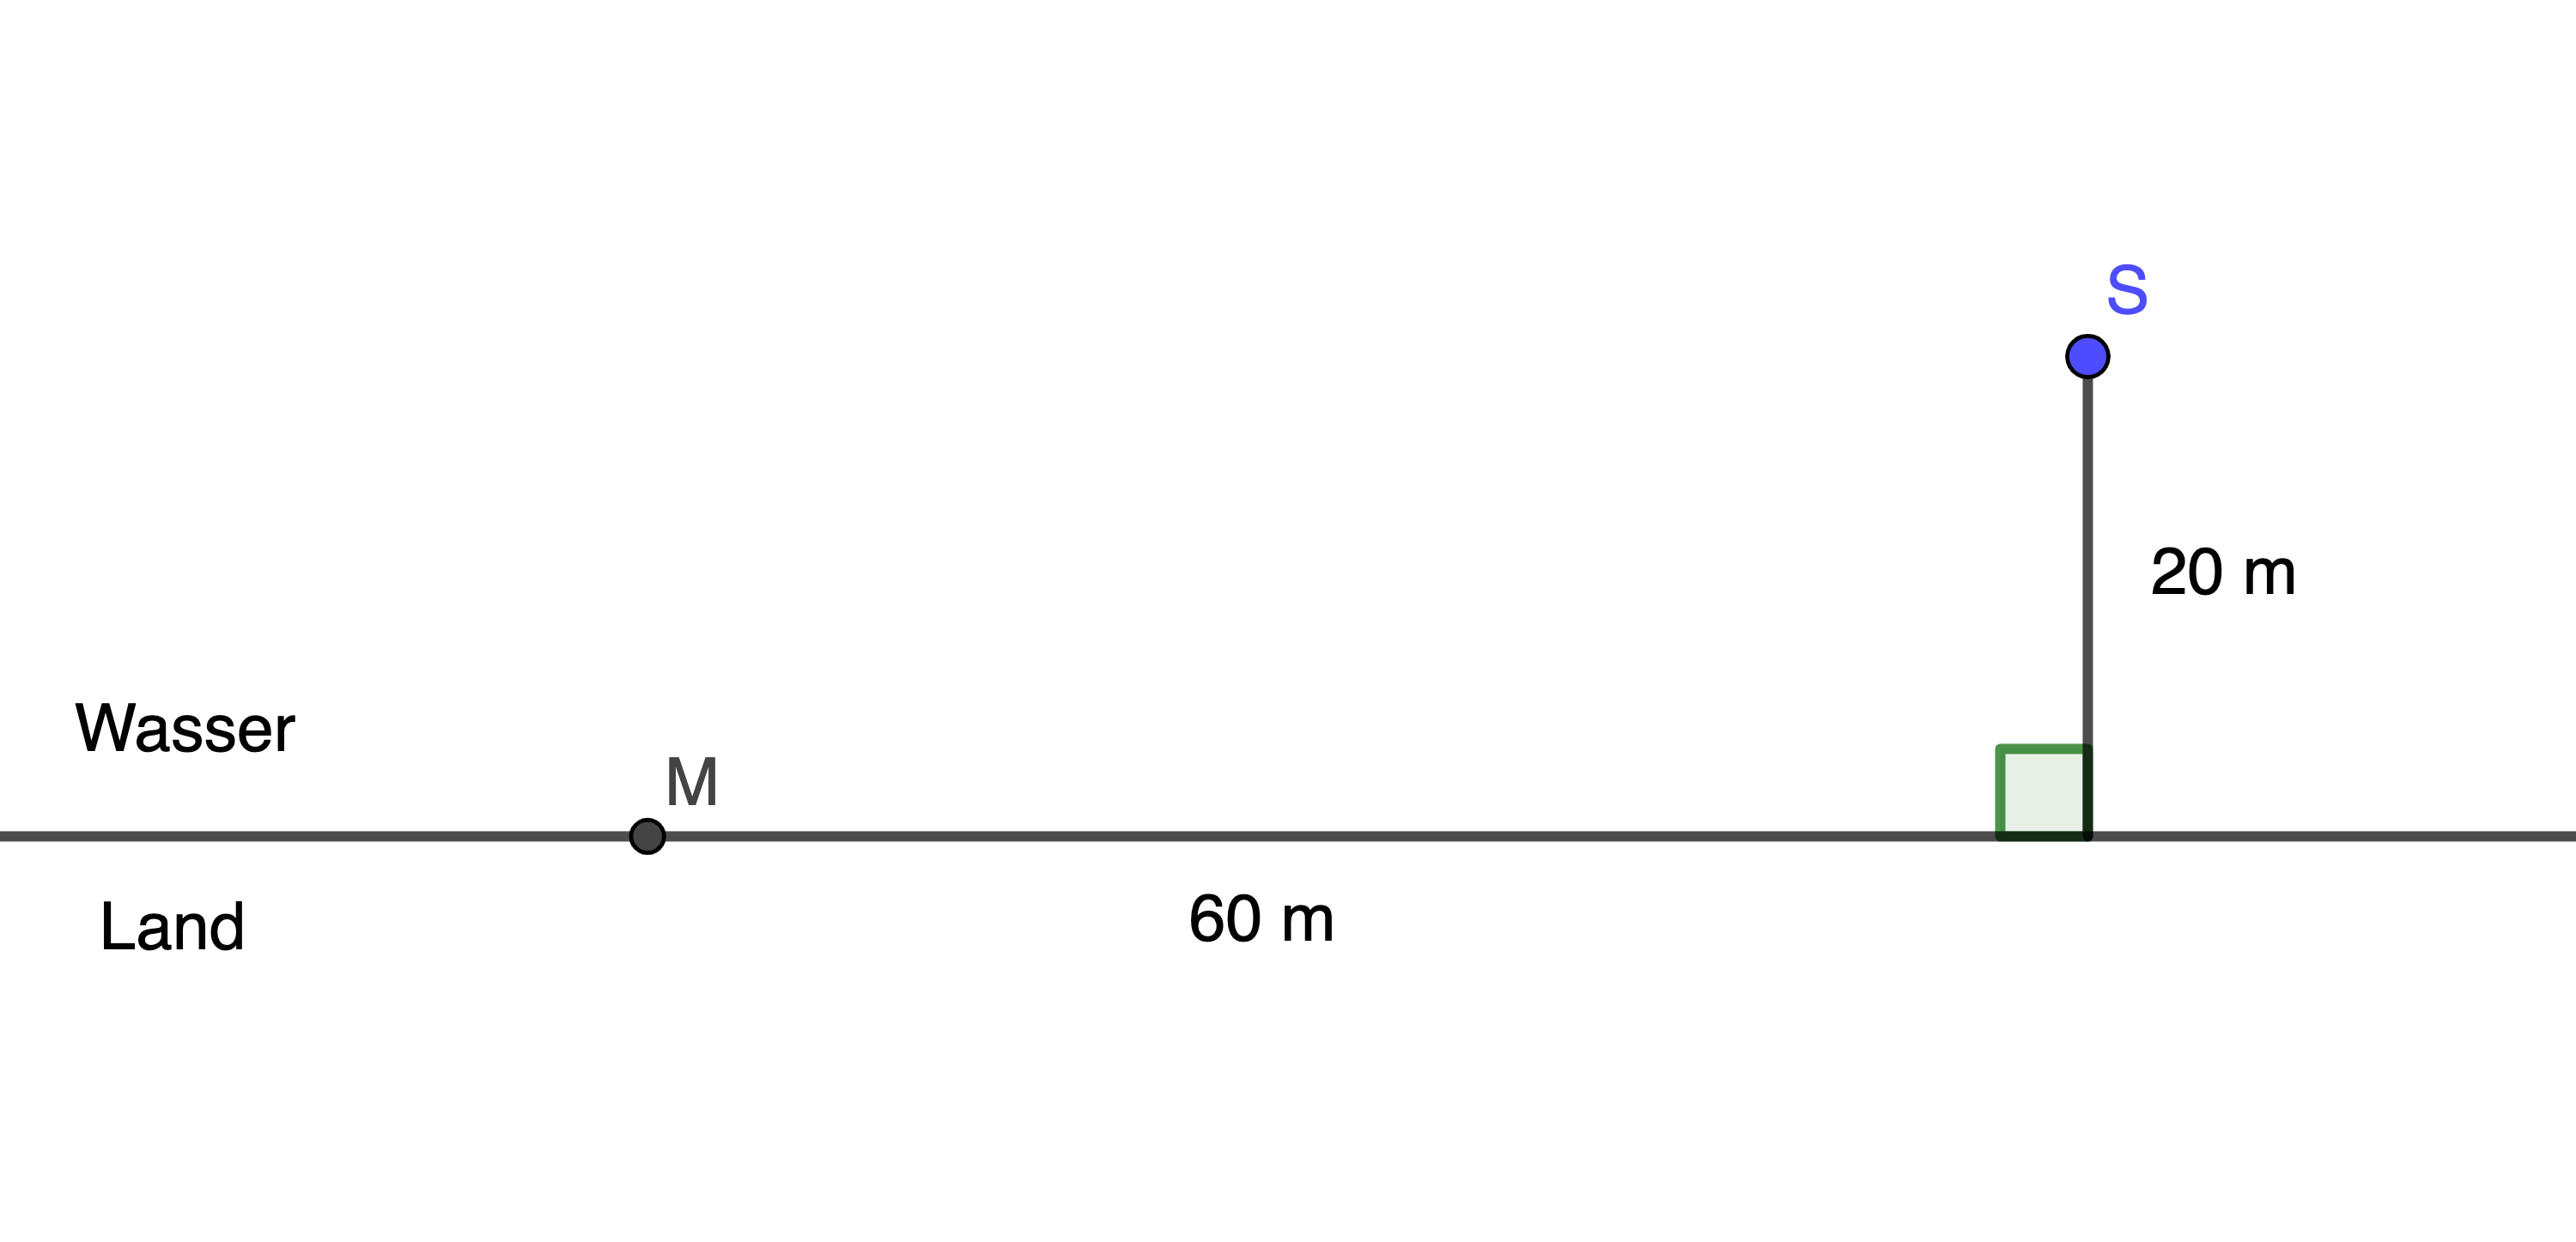
\includegraphics[width = 0.8 \textwidth]{media/baywatch.png}
	\end{center}
	\vspace*{10cm}
	\pagebreak
	\phantom{hallo}
	\vspace*{19cm}

\end{bsp}

\clearpage

\begin{bsp}
	{Bus optimal erwischen}{}
	Sie wohnen in der Entfernung 100 m von einer geraden Strasse. Jeden Morgen um 7Uhr fährt ein Bus mit der Geschwindigkeit 4 m/s vorbei, auf den Sie mit 2 m/s rennend jeweils aufspringen. In welchem Winkel $x$ zum Lot der Strasse müssen Sie jeweils losrennen, damit Sie möglichst spät von zu Hause wegrennen können?

	\vspace*{18 cm}

\end{bsp}

\clearpage

\begin{ueb}
	{}{}
	\begin{enumerate}
		\item Was vermuten Sie: Welches von allen gleichschenkligen Dreiecken mit dem Umfang 24\,cm hat den grössten Flächeninhalt? Beweisen Sie Ihre Vermutung, indem Sie das entsprechende Extremalproblem lösen. Hinweis: Sie können die Zielfunktion mit Produkt- und Kettenregel ableiten, oder Sie formen sie so um, dass Sie eine Ersatzfunktion verwenden können. Beides geht.
		\item Einem Rechteck wird ein gleichschenkliges Dreieck aufgesetzt (siehe Skizze). Wie breit muss das Rechteck sein, damit der Flächeninhalt der ganzen Figur maximal wird? Hinweis: Hier werden Sie vermutlich die Produkt- und die Kettenregel verwenden müssen. Vergessen Sie bei der Wurzelgleichung die Probe nicht.
		      \begin{center}
			      %% TikZ-Code fuer die dargestellte Figur

			      \begin{tikzpicture}[scale=2]
				      %% Untere Basis
				      \draw (0,0) -- (3,0);

				      %% Seitenwaende (Hoehe 1)
				      \draw (0,0) -- (0,1);
				      \draw (3,0) -- (3,1);

				      %% Schraegdaecher mit Laenge 2
				      %% %% Hinweis: Exakte Position des Firstpunkts im Bild unklar
				      %% %% daher angenommene symmetrische Position
				      \draw (0,1) -- (1.5,2);
				      \draw (3,1) -- (1.5,2);

				      %% Beschriftungen
				      \node[left] at (0,0.5) {1};
				      \node[right] at (3,0.5) {1};
				      \node[above] at (0.75,1.5) {2};
				      \node[above] at (2.25,1.5) {2};
			      \end{tikzpicture}

		      \end{center}



		\item $$f(x) = e^{-x^2}$$
		      \begin{enumerate}
			      \item Der Ursprung des Koordinatensystems ist die Spitze eines gleichschenkligen Dreiecks; die Endpunkte der Basis liegen auf dem Graphen von \(f\). Das Dreieck soll maximalen Flächeninhalt haben. Welche Koordinaten haben die Endpunkte der Basis?
			      \item Zeigen Sie, dass die in a. gefundenen Punkte den Wendepunkten der Funktion \(f\) entsprechen.
		      \end{enumerate}


		\item Die Punkte \(A(3,3)\) und \(B(0,2)\) sind gegeben. Der Punkt \(C\) liegt auf der Kurve \(f\colon y=\ln x\). Das Dreieck \(ABC\) soll minimalen Flächeninhalt haben. Welche Koordinaten hat \(C\)? Tipp: Hier empfiehlt sich ein ganz anderer Lösungsweg. Was kann man über die Kurventangente in $C$ sagen?

	\end{enumerate}

\end{ueb}

\clearpage
%% Kurzloesungen

\begin{enumerate}
	\item Seiten \(8,8,8\) (Gleichseitiges Dreieck).

	\item Rechteckbreite \(=2\sqrt{3}\).



	\item
	      \begin{enumerate}
		      \item Endpunkte \( P_{1,2} = (\pm \tfrac{1}{\sqrt{2}},\, e^{-1/2}) \).
		      \item Rechne nach: $f''(\pm \tfrac{1}{\sqrt{2}}) = 0$ und $f'''(\pm \tfrac{1}{\sqrt{2}}) \neq 0$.
	      \end{enumerate}
	\item Minimaler Flaecheninhalt des Dreiecks \(ABC\): Punkt \(C=(3,\ln(3))\).
\end{enumerate}

\clearpage

\begin{ueb}
	{Optimale Geschwindigkeit einer Autokolonne}{}
	% Zu hohes Verkehrsaufkommen auf einer engen Strasse \dots wieder ein Stau! Je grösser das Verkehrsaufkommen, desto langsamer bewegt sich die Autokolonne. Bei kleinen Geschwindigkeiten können mehr Autos passieren.

	% Diese Feststellung ist insofern etwas eigenartig, als bei 0 km/h überhaupt kein Auto fährt. Gibt es eine optimale Geschwindigkeit für eine Autokolonne?

	Wichtig bei Autokolonnen ist der Sicherheitsabstand zwischen Fahrzeugen. Je grösser die Geschwindigkeit der Kolonne, desto grösser muss der Abstand sein und das hat einen Einfluss auf den Durchfluss. Umgekehrt ist der Abstand bei kleinen Geschwindigkeiten klein, aber im Schneckentempo ist der Durchfluss auch nicht gerade gross.
	Eine Faustregel der Polizei sagt:
	\[r\approx0.0075 v^2 \quad \text{$v$ in km/h, $r=$ Bremsweg in m}\]

	\begin{enumerate}
		\item Wie viele Meter Abstand zum vorderen Fahrzeug müsste eine Automobilistin bei einer Geschwindigkeit von 60 km/h mindestens einhalten?
		\item Stellen Sie sich vor, eine Kolonne habe eine Geschwindigkeit von 60 km/h und bestehe aus lauter Personenwagen. Der Einfachheit halber nehmen wir an, dass jedes Auto eine Länge von 4 m habe und dass alle Automobilistinnen und Automobilisten den vorgeschriebenen Abstand einhalten.
		      An einer gewissen Stelle hat die Polizei eine Zählstation aufgestellt.
		      \begin{center}
			      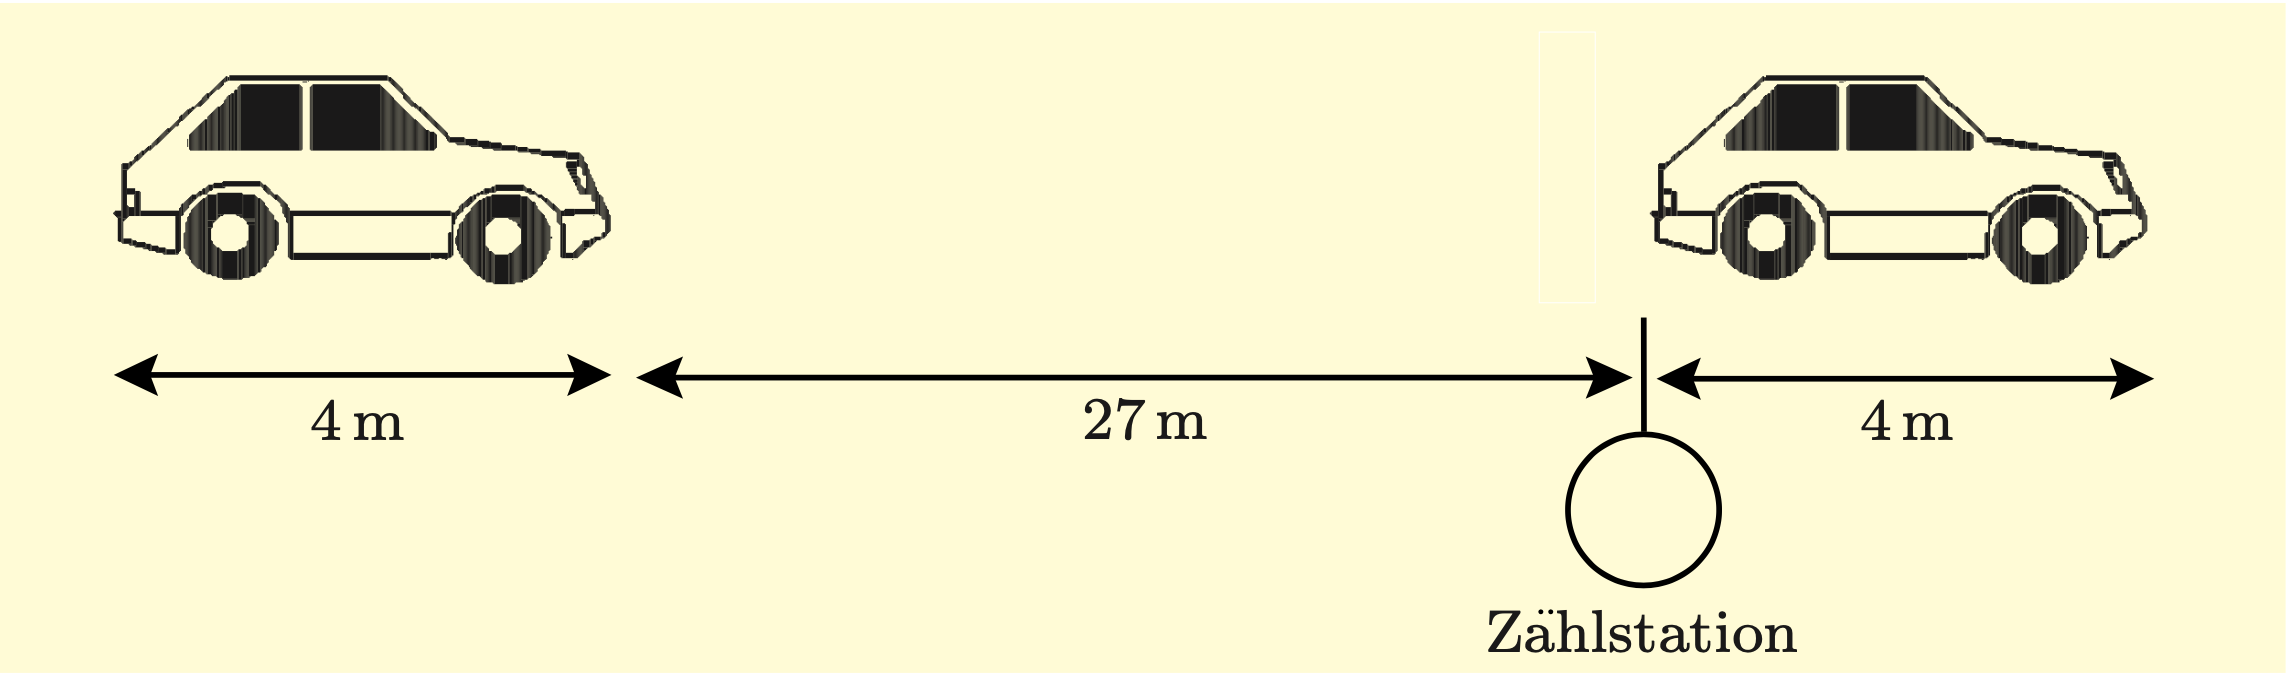
\includegraphics[width = 0.8 \textwidth]{media/auto-zaehlstation-neu.png}
		      \end{center}
		      Zeigen Sie, dass pro Minute ungefähr 32 Autos vorbeifahren können.
		\item Wie viele Autos können bei einer Geschwindigkeit von 120 km/h bei der Zählstation vorbeifahren?
		\item Die Anzahl Autos $N$, welche die Zählstation pro Minute passieren können, ist eine Funktion der Geschwindigkeit $v$ in km/h.
		      \\ Zeigen Sie, dass gilt
		      \[ N(v)=\frac{1000v}{0.45v^2+240}\]
		\item Zeichnen Sie den Graphen der Funktion mit Geogebra und kontrollieren Sie, dass der maximale Durchfluss einer Kolonne unter den oben skizzierten Bedingungen bei ungefähr 25 km/h liegt.
		\item Berechnen Sie $\frac{dN}{dv}$ und benutzen Sie das Resultat, um die optimale Geschwindigkeit auszurechnen.
		\item Wie beurteilen Sie das Modell? Machen Sie Vorschläge für Verbesserungen und Untersuchen Sie die daraus resultierende optimale Geschwindigkeit.

	\end{enumerate}

\end{ueb}

\clearpage



\section{Integralrechnung}
\subsection{Stammfunktionen und unbestimmtes Integral}
\begin{LA}
	{Momentane Position}{}
	Wir denken uns ein Massband, das entlang der 100-Meter-Bahn der KS Im Lee ausgelegt ist. Die Position $s=0$ befindet sich an der Startlinie, die Position $s=100$ an der Ziellinie.

	Alice programmiert einen Roboter so, dass seine Position $s(t)$ in Metern zu jeder Zeit $t$ in Sekunden durch die Funktion
	$$s_A (t) = t^2 + 5$$
	beschrieben wird.

	\begin{enumerate}
		\item Wo auf der Bahn wird der Roboter von Alice zum Zeitpunkt $t=0$ positioniert?
		\item Bestimmen Sie die momentante Geschwindigkeit $v_A (t)$ des Roboters von Alice.
		\item Was ändert sich an den Funktionen $s_A (t)$ und $v_A (t)$, wenn Alice den Roboter zum Zeitpunkt $t=0$ an der Startlinie losfahren lässt?
	\end{enumerate}

	Auch Bob testet einen Roboter. Dieser wird auf die Bahn gesetzt und beschleunigt schnell in Richtung Ziellinie. Während der Fahrt wird der Roboter immer schneller. Seine momentane Geschwindigkeit $v_B(t)$ in Meter pro Sekunde ist durch die Funktion
	$$v_B(t) = \frac{1}{2} t^2 + t$$
	gegeben, wobei $t$ die Zeit in Sekunden seit dem Start angibt.

	\begin{enumerate}
		\item Bestimmen Sie die Funktion $s_B(t)$, welche die momentane Position des Roboters in Metern angibt. Gehen Sie davon aus, dass der Roboter zum Zeitpunkt $t=0$ an der Startlinie steht, also $s_B(0)=0$ gilt.
		\item Wie lautet die Funktion $s_B(t)$, wenn der Roboter zum Zeitpunkt $t=0$ bereits 5 Meter von der Startlinie entfernt ist, also $s_B(0)=5$ gilt?
	\end{enumerate}

\end{LA}


\clearpage
\begin{definition}
	{Stammfunktion}{}
	Sei $f$ eine auf einem Intervall $\DD$ definierte Funktion. Eine Funktion $F$ heisst Stammfunktion von $f$, wenn für alle $x \in \DD$ gilt
	$$F'(x) = f(x)$$

\end{definition}

\begin{bsp}
	{Stammfunktionen von $\sin(x)$}{}
	$f(x) = \sin(x)$

	\vspace*{5cm}
\end{bsp}

\begin{definition}
	{Unbestimmtes Integral}{}
	Sei $f$ eine auf einem Intervall $\DD$ definierte Funktion. Das unbestimmte Integral von $f$ ist die Menge aller Stammfunktionen von $f$ und wird mit
	$$\int f(x) \, dx$$
	bezeichnet.

	Wenn $F$ eine Stammfunktion von $f$ ist, so wird das unbestimmte Integral so angegeben:
	$$\int f(x) \, dx = F(x) + C$$
	wobei $C \in \R$ eine Konstante ist.
\end{definition}

Das Suchen nach einer Stammfunktion wird als \textit{Integrieren} oder \textit{Antidifferentieren} bezeichnet. Das Integrieren ist also die Umkehrung des Ableitens – genauso wie das Wurzelziehen die Umkehrung des Quadrierens ist.

\begin{bsp}
	{Unbestimmte Integrale}{}

	\begin{itemize}
		\item $\int x^2 \, dx = $

		      \vspace*{1cm}

		\item $\int \left( \cos(x) + \frac{1}{x^2}\right) \, dx = $

		      \vspace*{1cm}

	\end{itemize}


\end{bsp}

\clearpage

\begin{satz}
	{Erste Integrationsregeln}{}
	\begin{enumerate}
		\item Potenzregeln: für $n \neq -1$ gilt:
		      $$ \int x^n \, dx = \frac{x^{n+1}}{n+1} + C $$
		\item Summenregel:
		      $$ \int (f(x) + g(x)) \, dx = \int f(x) \, dx + \int g(x) \, dx $$
		\item Faktorregel: Für einen konstanten Faktor $k$ gilt:
		      $$ \int k \cdot f(x) \, dx = k \cdot \int f(x) \, dx $$
	\end{enumerate}
\end{satz}

Diese Regeln sind eine direkte Folge der entsprechenden Ableitungsregeln.

\begin{ueb}
	{}{}
	Tipp: Das Bestimmen der Integrale geschieht häufig durch Versuch und Irrtum. Man überlegt sich einen möglichen Kandidaten für die Stammfunktion und leitet diesen ab, um zu überprüfen, ob man die gegebene Funktion erhält. Falls nicht, hat man häufig eine Idee gewonnen, wie man den Kandidaten anpassen muss.


	\begin{enumerate}
		\item Bestimmen Sie die folgenden unbestimmten Integrale:
		      \begin{enumerate}
			      \item $\int 7 \, dx$
			      \item $\int x^5 \, dx$
			      \item $\int (2x^{-3} -4x^3) \, dx$
			      \item $\int \sqrt{x} \, dx$
			      \item $\int (x-3) \cdot \sqrt{x} \, dx$
		      \end{enumerate}
		\item Bestimmen Sie die folgenden unbestimmten Integrale mit etwas schwierigeren Funktionen:
		      \begin{enumerate}
			      \item $\int \cos(x) \, dx$
			      \item $\int e^x \, dx$
			      \item $\int \frac{1}{x} \, dx \quad , x>0$
			      \item $\int \sin(2x) \, dx$
			      \item $\int \sqrt{3-x} \, dx$
		      \end{enumerate}
		\item Finden Sie eine Funktion $f$ sodass gilt:
		      \begin{enumerate}
			      \item $\int f(x) \, dx = x^2+5x+C$
			      \item $\int f(x) \, dx = x\cdot e^x + C$
			      \item $\int f(x) \, dx = 2 \cos^2(x) +C$
			      \item $\int f(x) \, dx = \frac{x^2}{3x+1} + C$
		      \end{enumerate}
	\end{enumerate}


\end{ueb}
\clearpage
\emph{Lösungen}
\begin{enumerate}
	\item  Integrale bestimmen:
	      \begin{enumerate}
		      \item $7x + C$
		      \item $\frac{1}{6} x^6 + C$
		      \item $-x^{-2} - x^4 + C$
		      \item $\frac{2}{3} x^{3/2} + C$
		      \item $ (x-3) \cdot \sqrt{x} = x^{3/2} - 3x^{1/2} \Rightarrow \int (x-3) \cdot \sqrt{x} \, dx = \frac{2}{5} x^{5/2} - 2 x^{3/2} + C$
	      \end{enumerate}
	\item Integrale bestimmen (schwierigere Funktionen):
	      \begin{enumerate}
		      \item $\sin(x) + C$
		      \item $e^x + C$
		      \item $\ln(x) + C$
		      \item $-\frac{1}{2} \cos(2x) + C$ (Der Vorfaktor eliminiert den Faktor 2, der durch die Kettenregel beim Ableiten entsteht.)
		      \item $-\frac{2}{3} (3-x)^{3/2} + C$ (Der Vorfaktor eliminiert den Faktor $-1$, der durch die Kettenregel beim Ableiten entsteht.)
	      \end{enumerate}
	\item Die Funktion rechts ist jeweils die Stammfunktion von $f$. Also muss $f$ die Ableitung der Funktion rechts sein.
	      \begin{enumerate}
		      \item $f(x) = 2x + 5$
		      \item $f(x) = e^x + x \cdot e^x$ (Produktregel)
		      \item $f(x) = -4 \cos(x) \cdot \sin(x)$ (Kettenregel)
		      \item $f(x) = \frac{3x^2+2x}{(3x+1)^2}$ (Quotientenregel)
	      \end{enumerate}
\end{enumerate}
\clearpage

\subsection{Flächenberechnung mit Ober- und Untersummen}
\subsubsection{Einführungsaufgaben}
Fragestellung: Wie bestimmt man den Flächeninhalt eines Gebietes, dessen Rand eine „gekrümmte Linie“ ist?
\begin{center}
	\includegraphics{media/flächeAllgemein.png}
\end{center}
Um uns an die Lösung dieses Problems zu nähern, reduzieren wir zunächst ein wenig die Schwierigkeit: Gegeben sei eine Funktion $f$, und ein Intervall $[a,b]$. Wir betrachten nun das Gebiet, das durch den Graphen von $f$, die $x$-Achse und die Geraden $x=a$ und $x=b$ berandet wird. Wie gross ist der Flächeninhalt $A$?
\begin{center}
	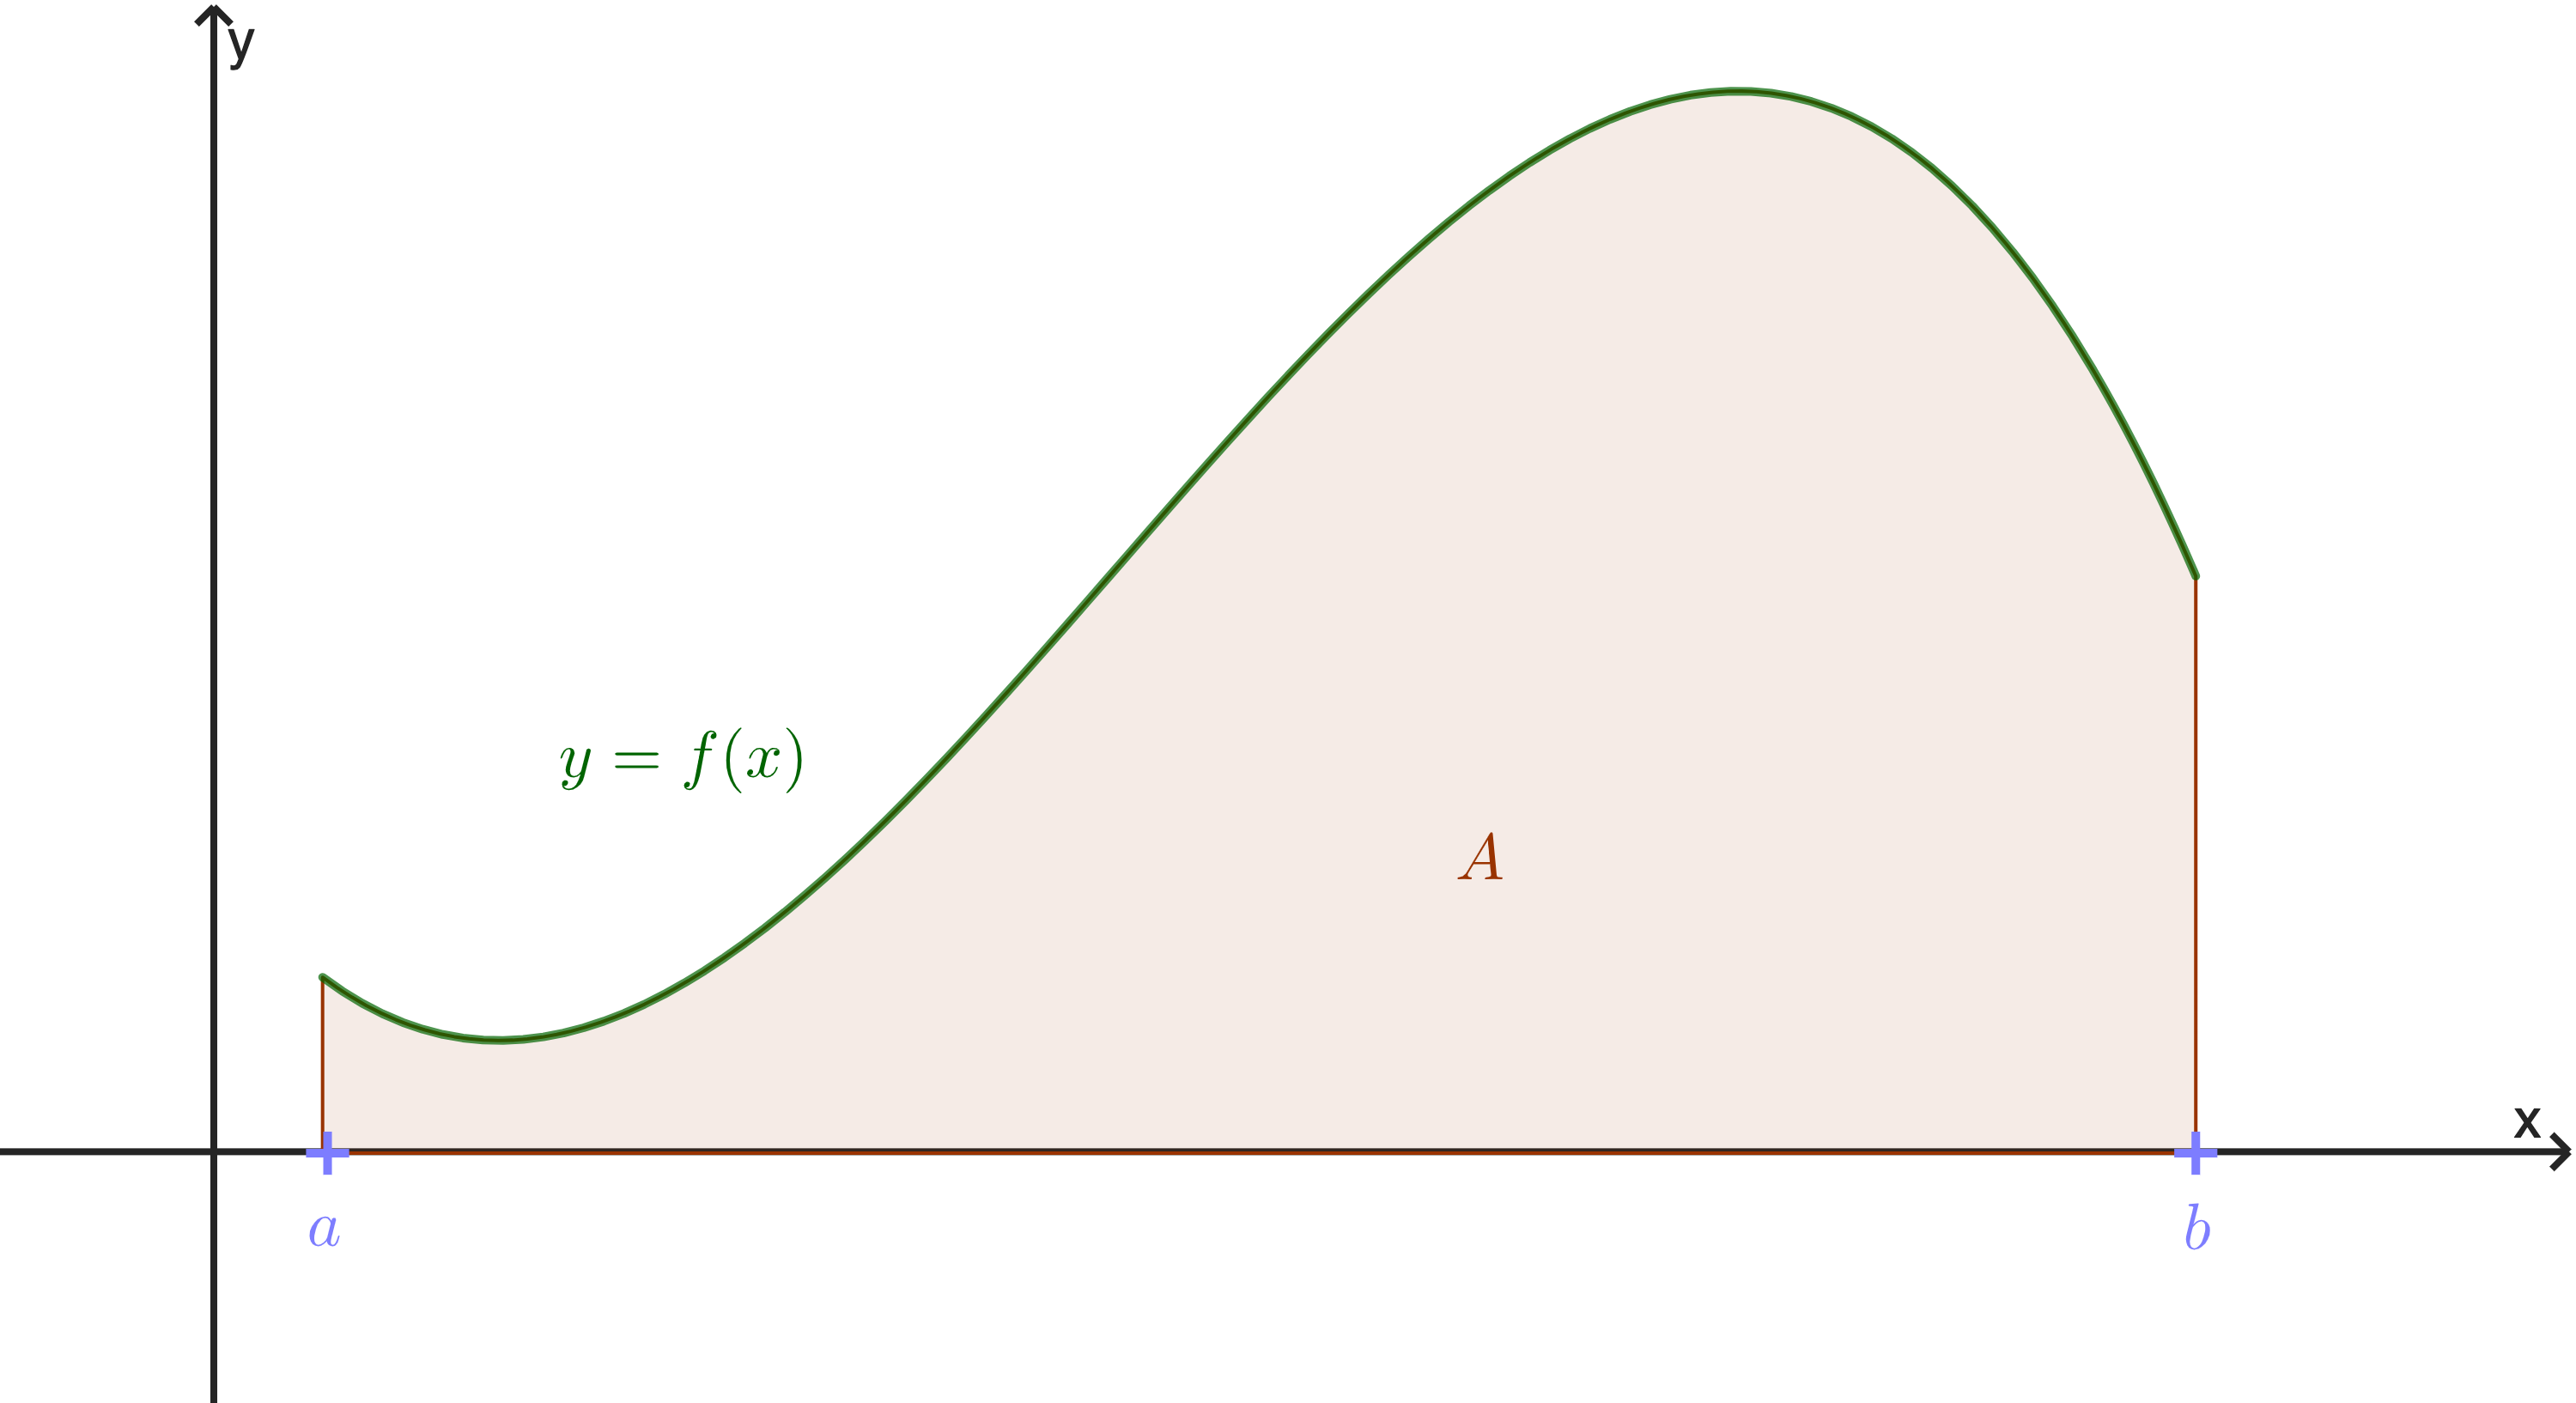
\includegraphics[width = 0.5\textwidth]{media/bestIntegral.png}
\end{center}
\clearpage
\begin{LA}{Einführungsaufgaben}{}
	Wenn die Funktion $f$ linear ist, können wir solche Flächeninhalte schon angeben.
	Berechnen Sie die schraffierten Flächeninhalte:
	\begin{enumerate}
		\item

		      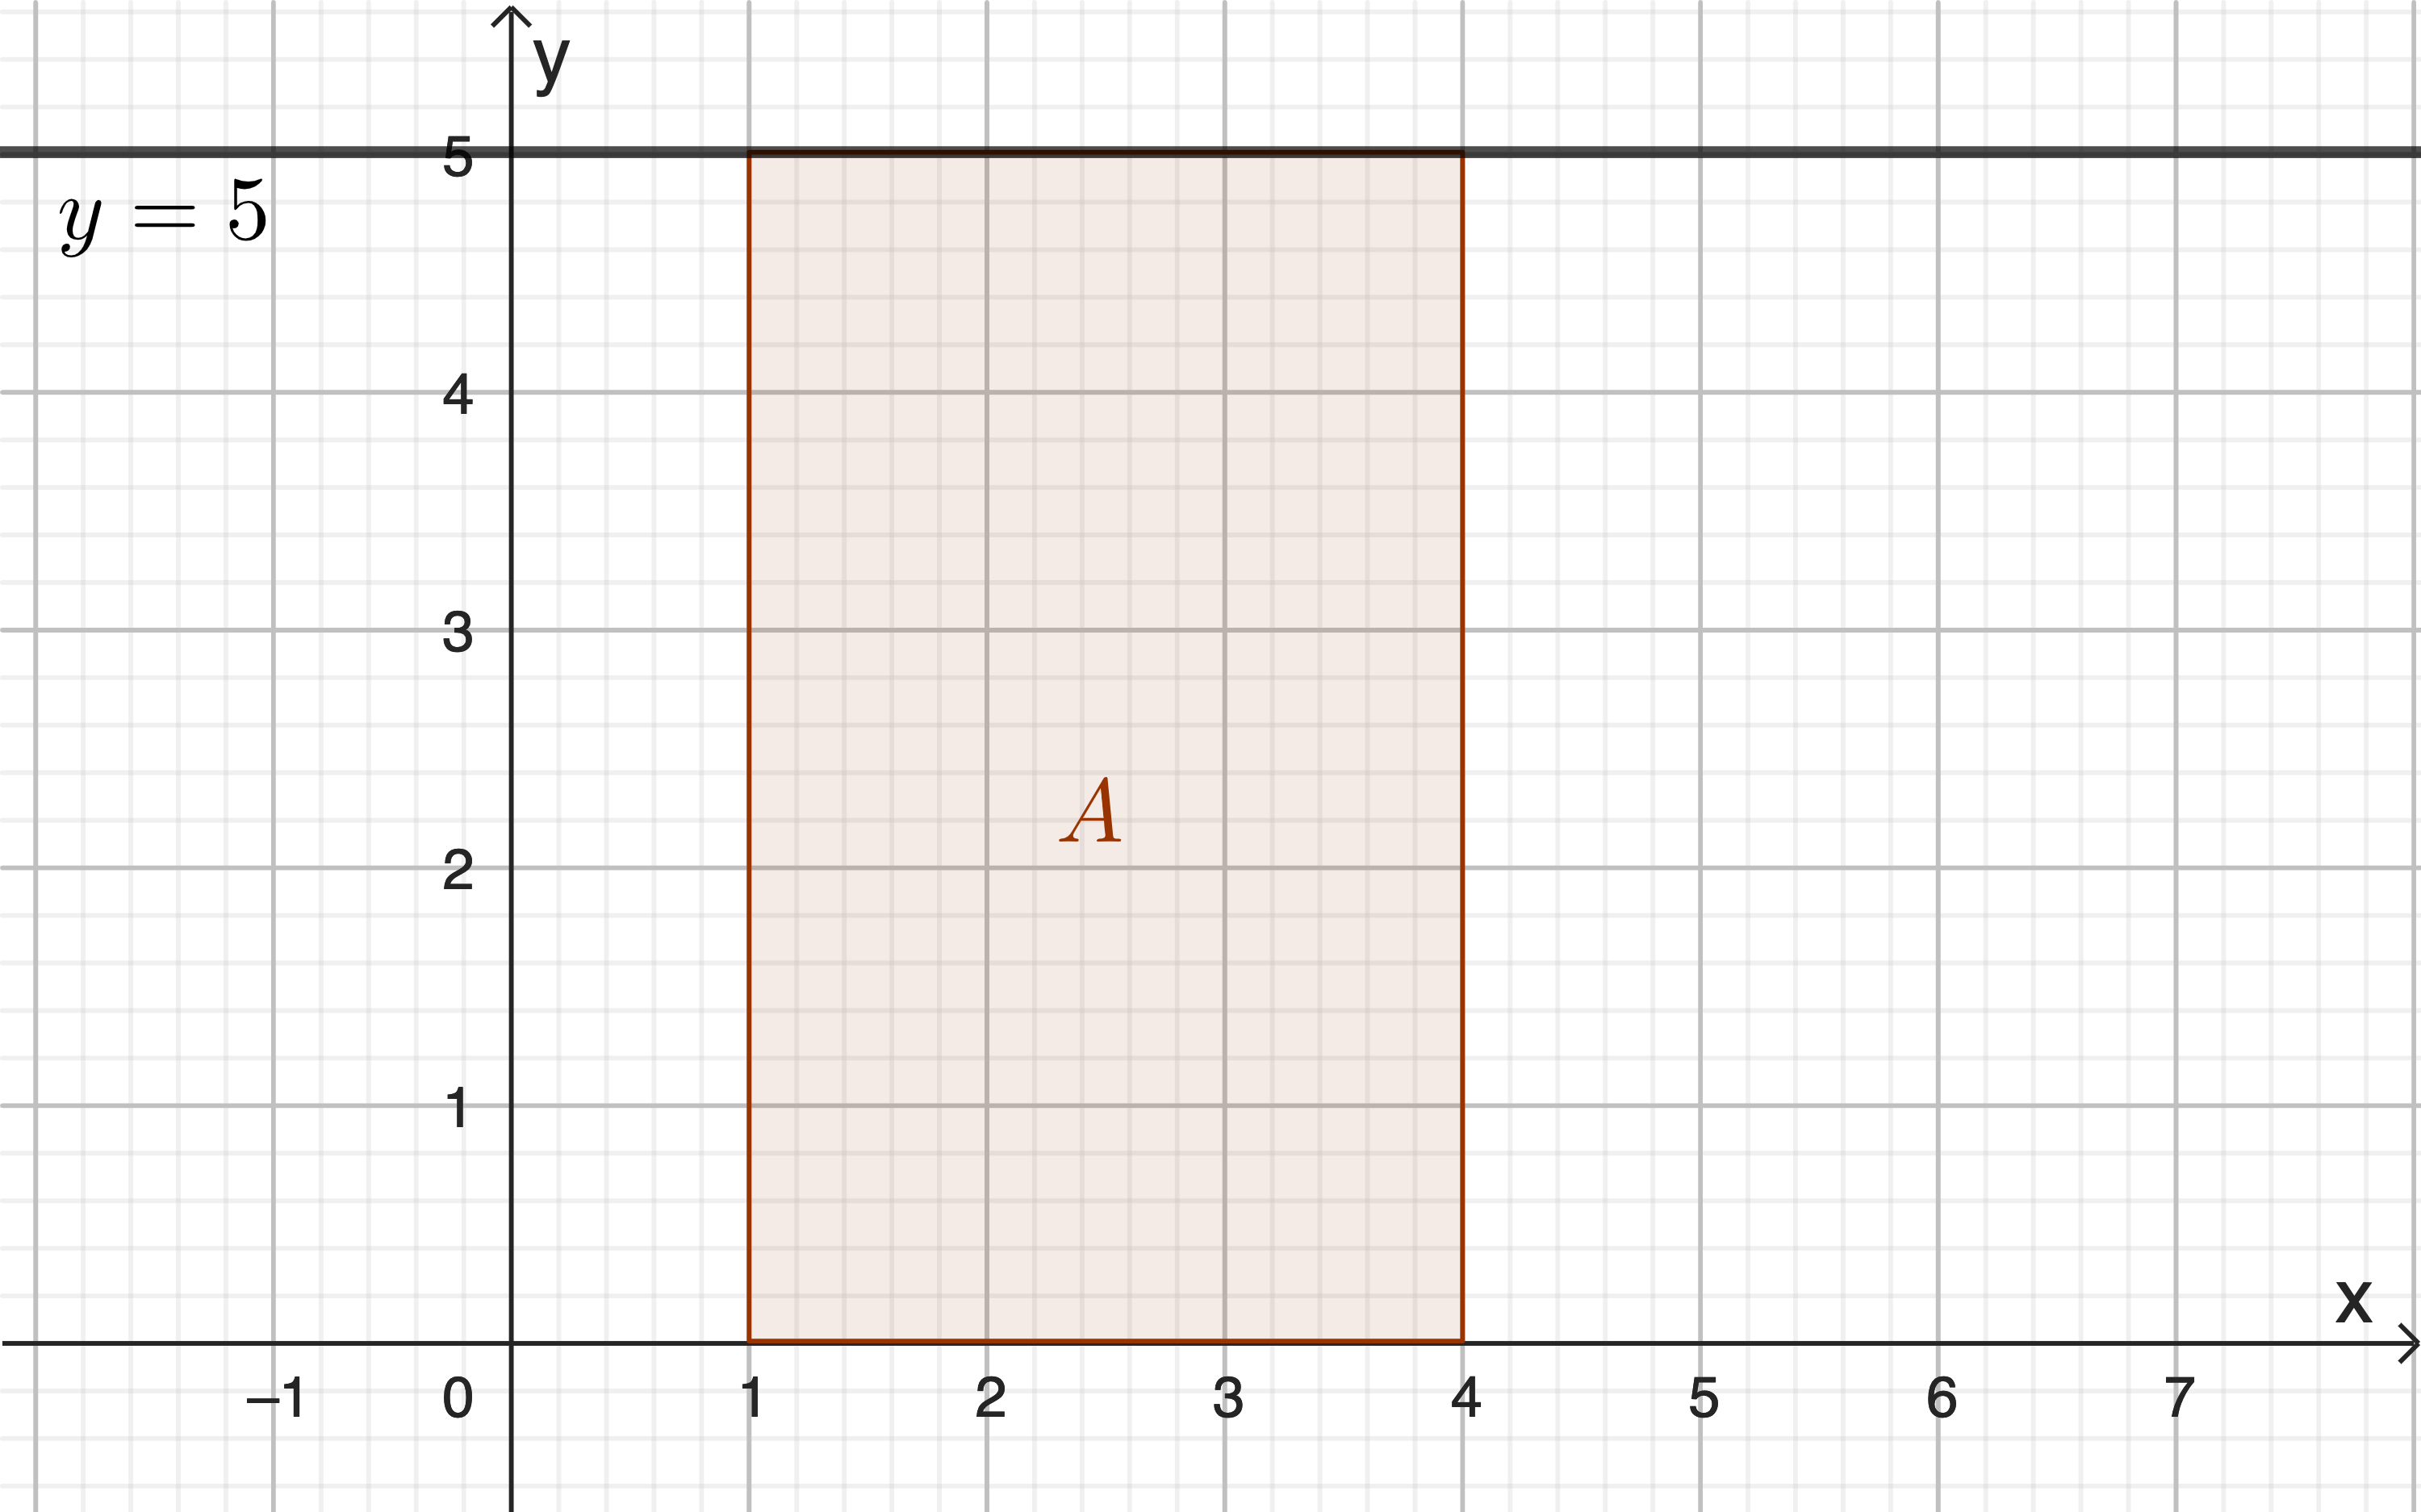
\includegraphics[width = 0.5\textwidth]{media/E-Bestimmt-Bsp1.png}
		\item

		      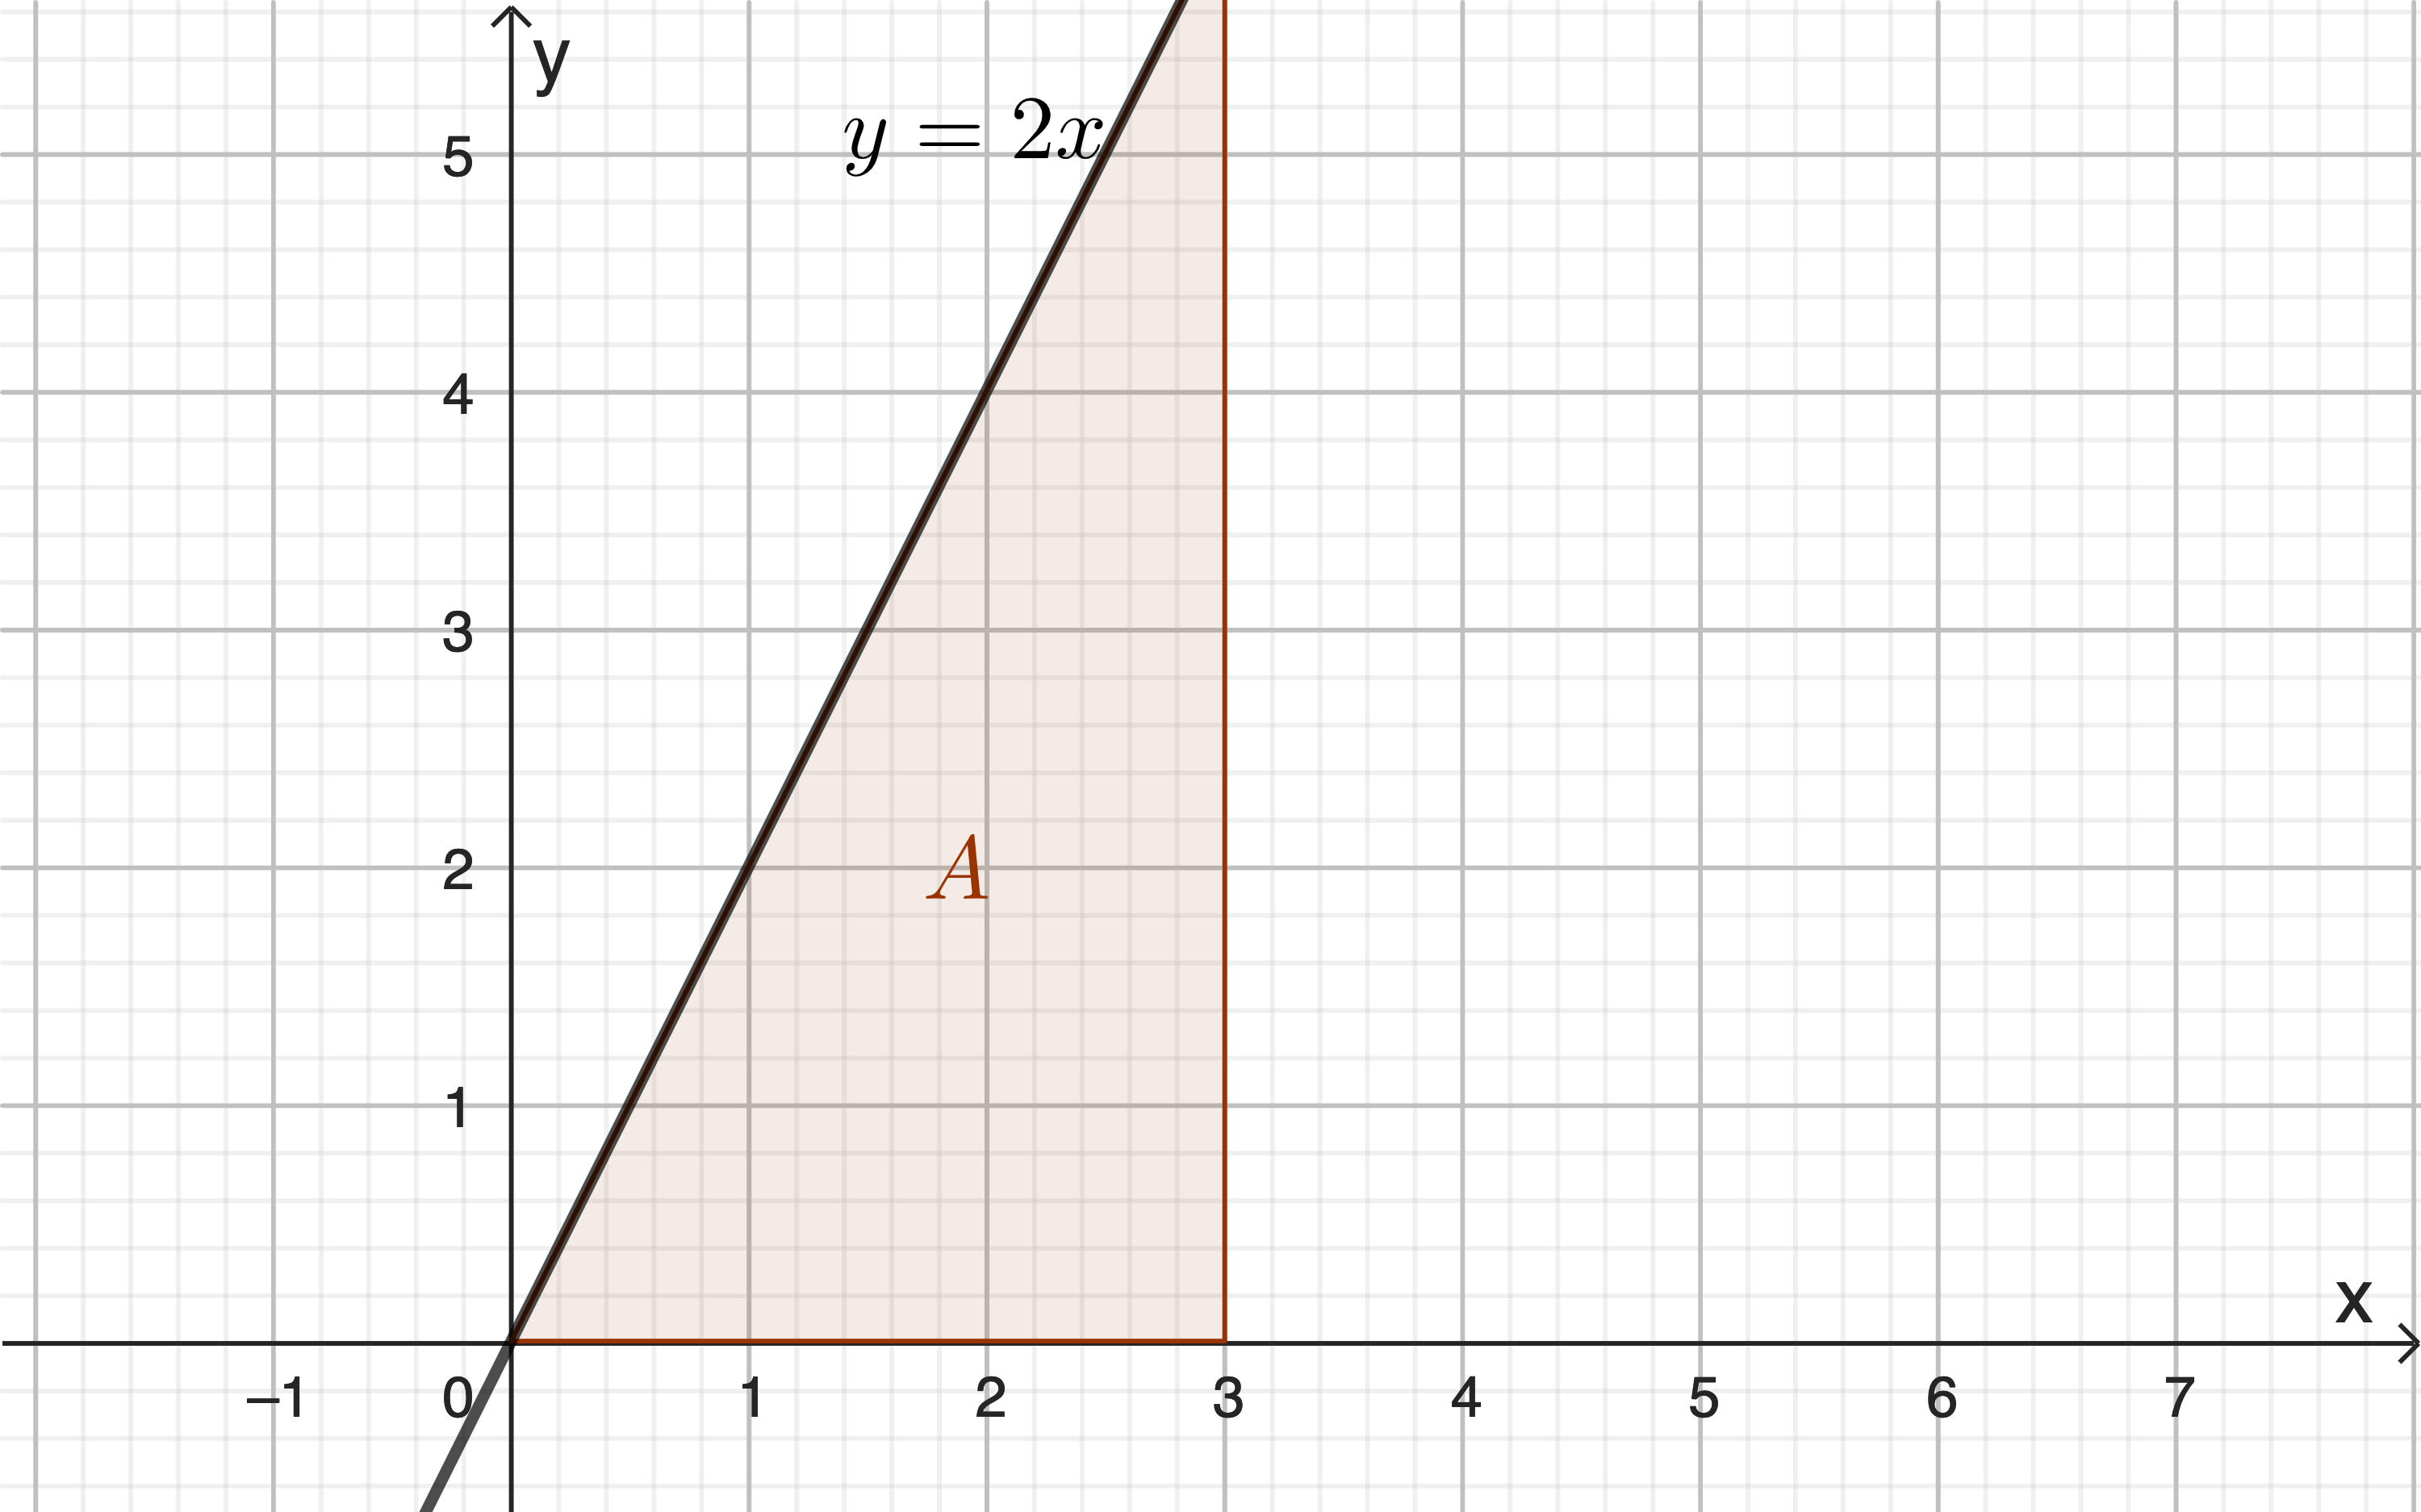
\includegraphics[width = 0.5\textwidth]{media/E-Bestimmt-Bsp2.png}
		\item

		      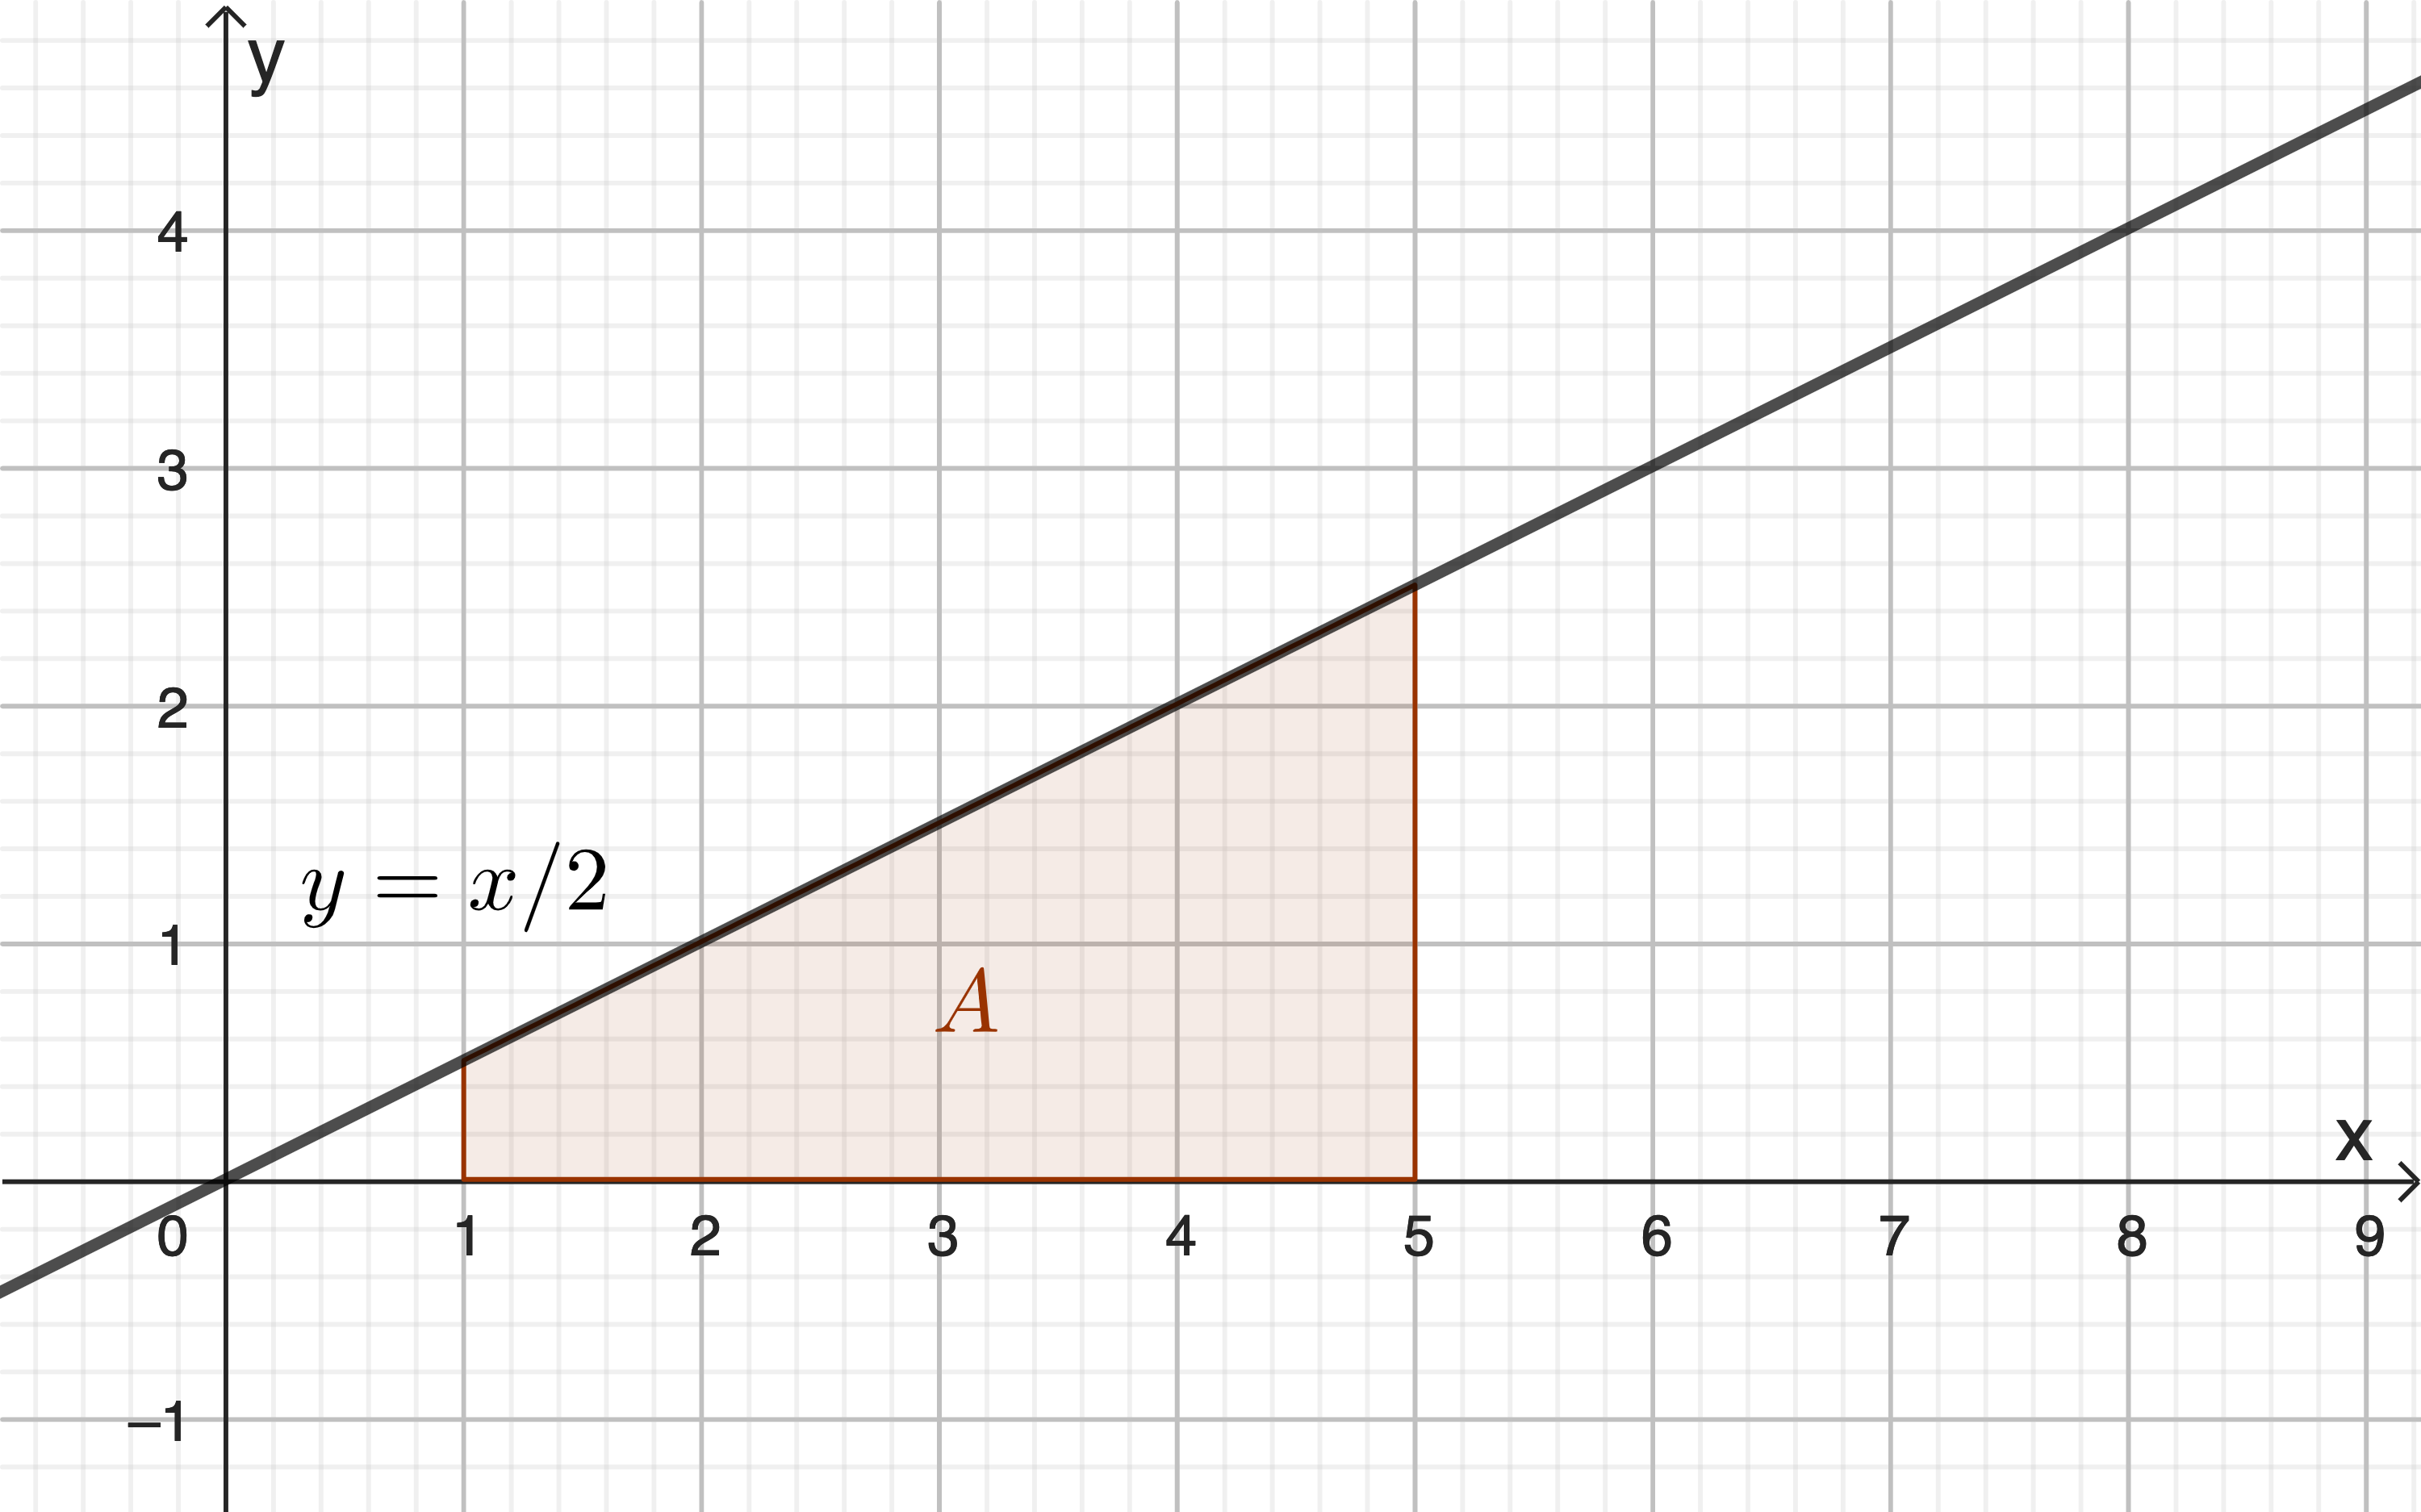
\includegraphics[width = 0.5\textwidth]{media/E-Bestimmt-Bsp3.png}
	\end{enumerate}

\end{LA}
\clearpage
Weil die Flächen in der Einführungsaufgabe durch geraden begrenzt sind, können die Flächeninhalte mit Hilfe von einfachen geometrischen Figuren berechnet werden. Anders sieht es aus, wenn die Fläche durch eine gekrümmte Linie begrenzt wird. Als Beispiel betrachten wir die Fläche unter dem Graphen der Funktion $f(x)=x^2$ im Intervall $[0, 1]$.

\begin{center}
	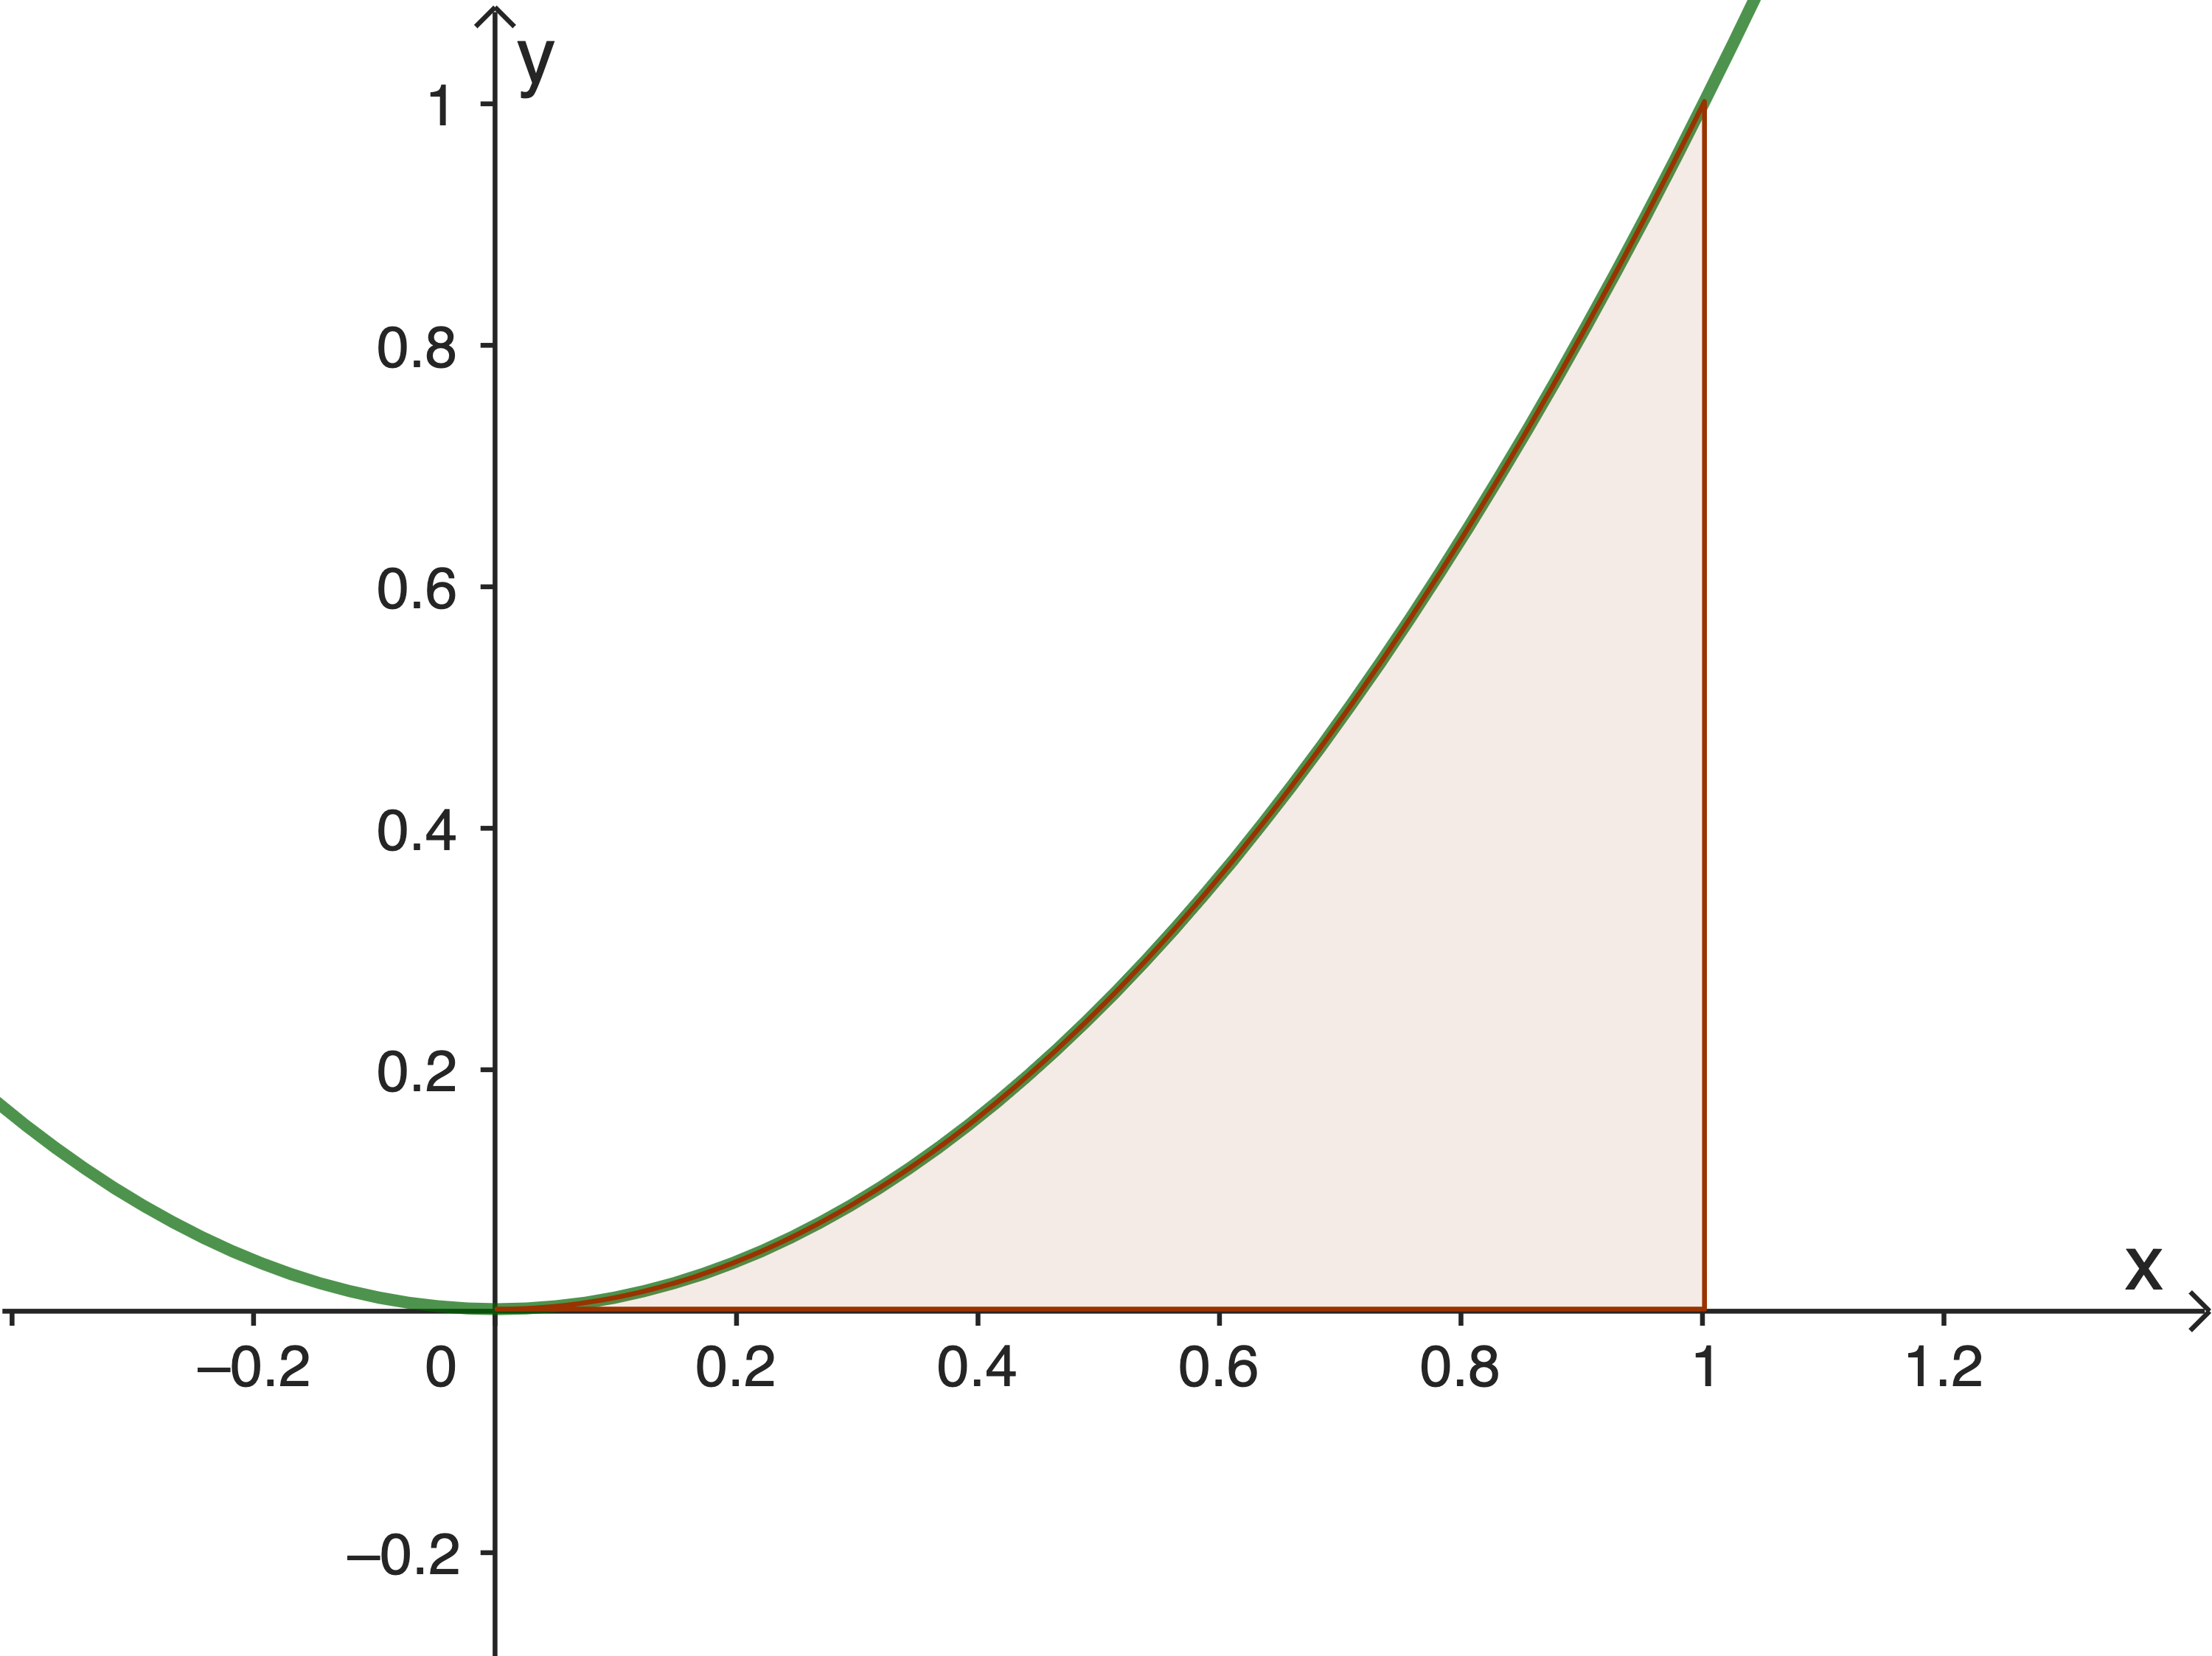
\includegraphics[width = 0.5\textwidth]{media/ober-untersumme-xquadrat.png}
\end{center}
Idee: Zur Bestimmung des Flächeninhalts unter der Parabel teilen wir das Intervall $[0,1]$ in vier Teile und betrachten zwei Näherungen für den Flächeninhalt.
\begin{center}
	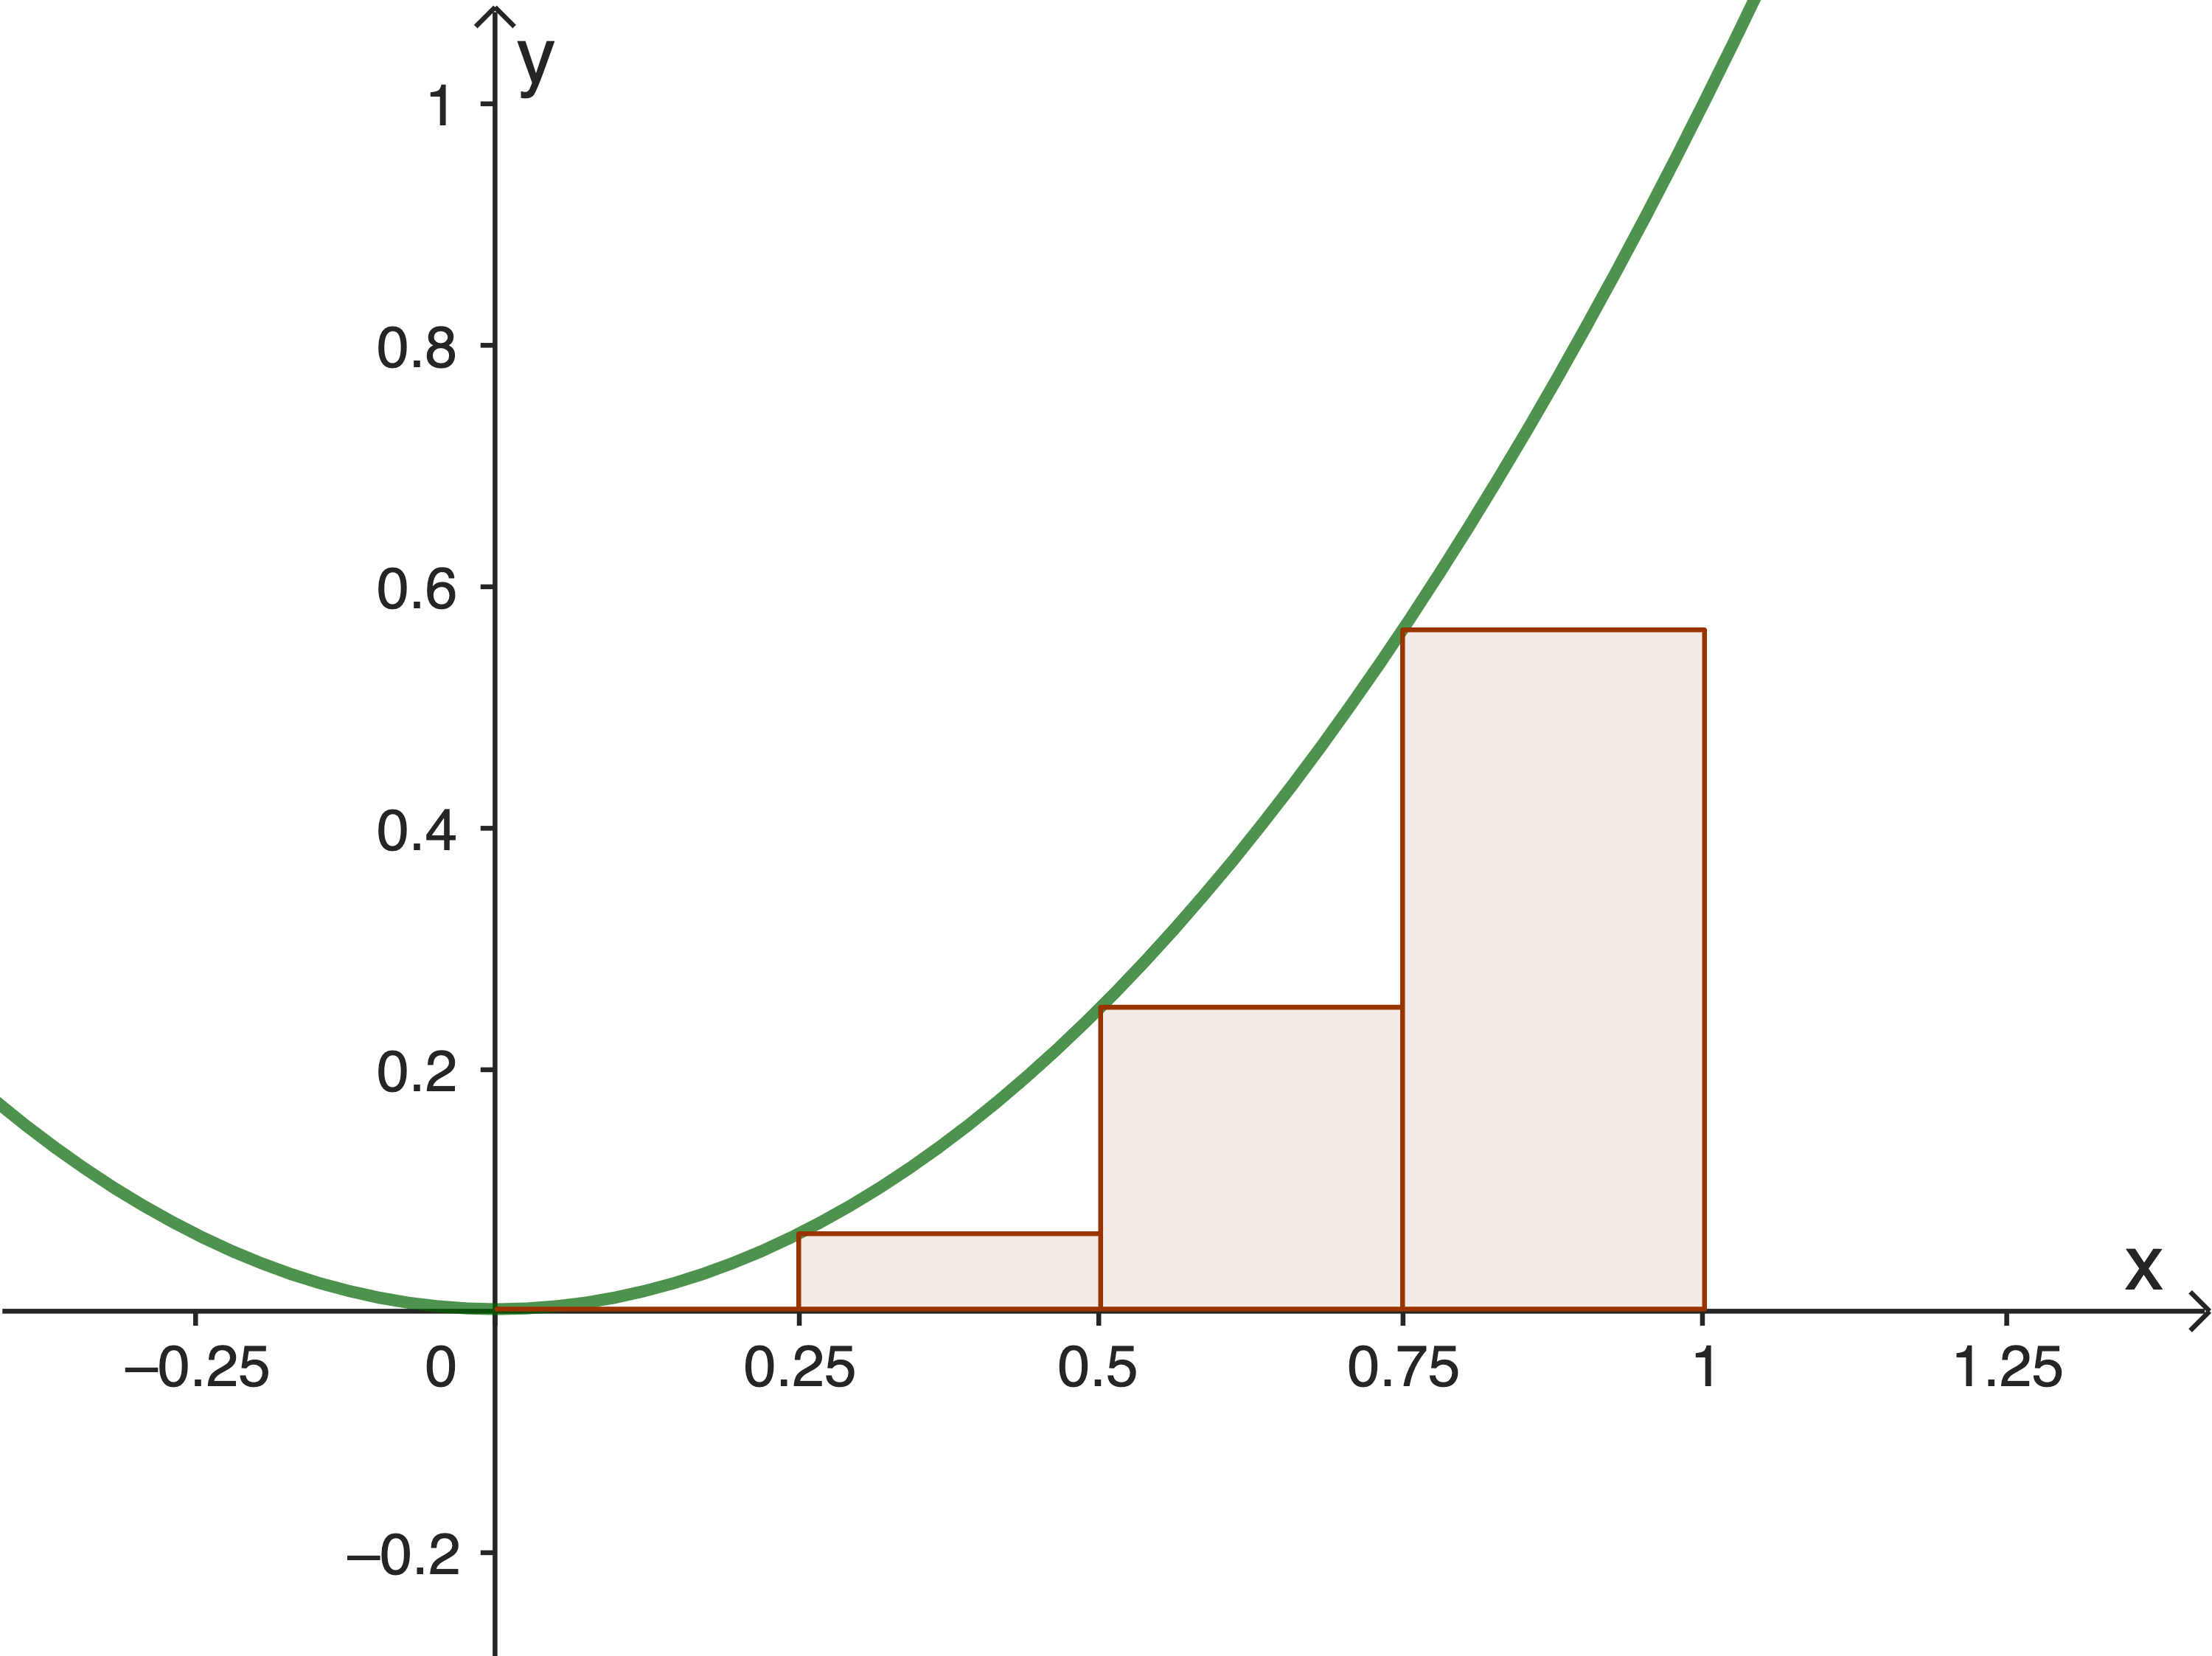
\includegraphics[width = 0.4\textwidth]{media/untersumme-x-quadrat.png}
	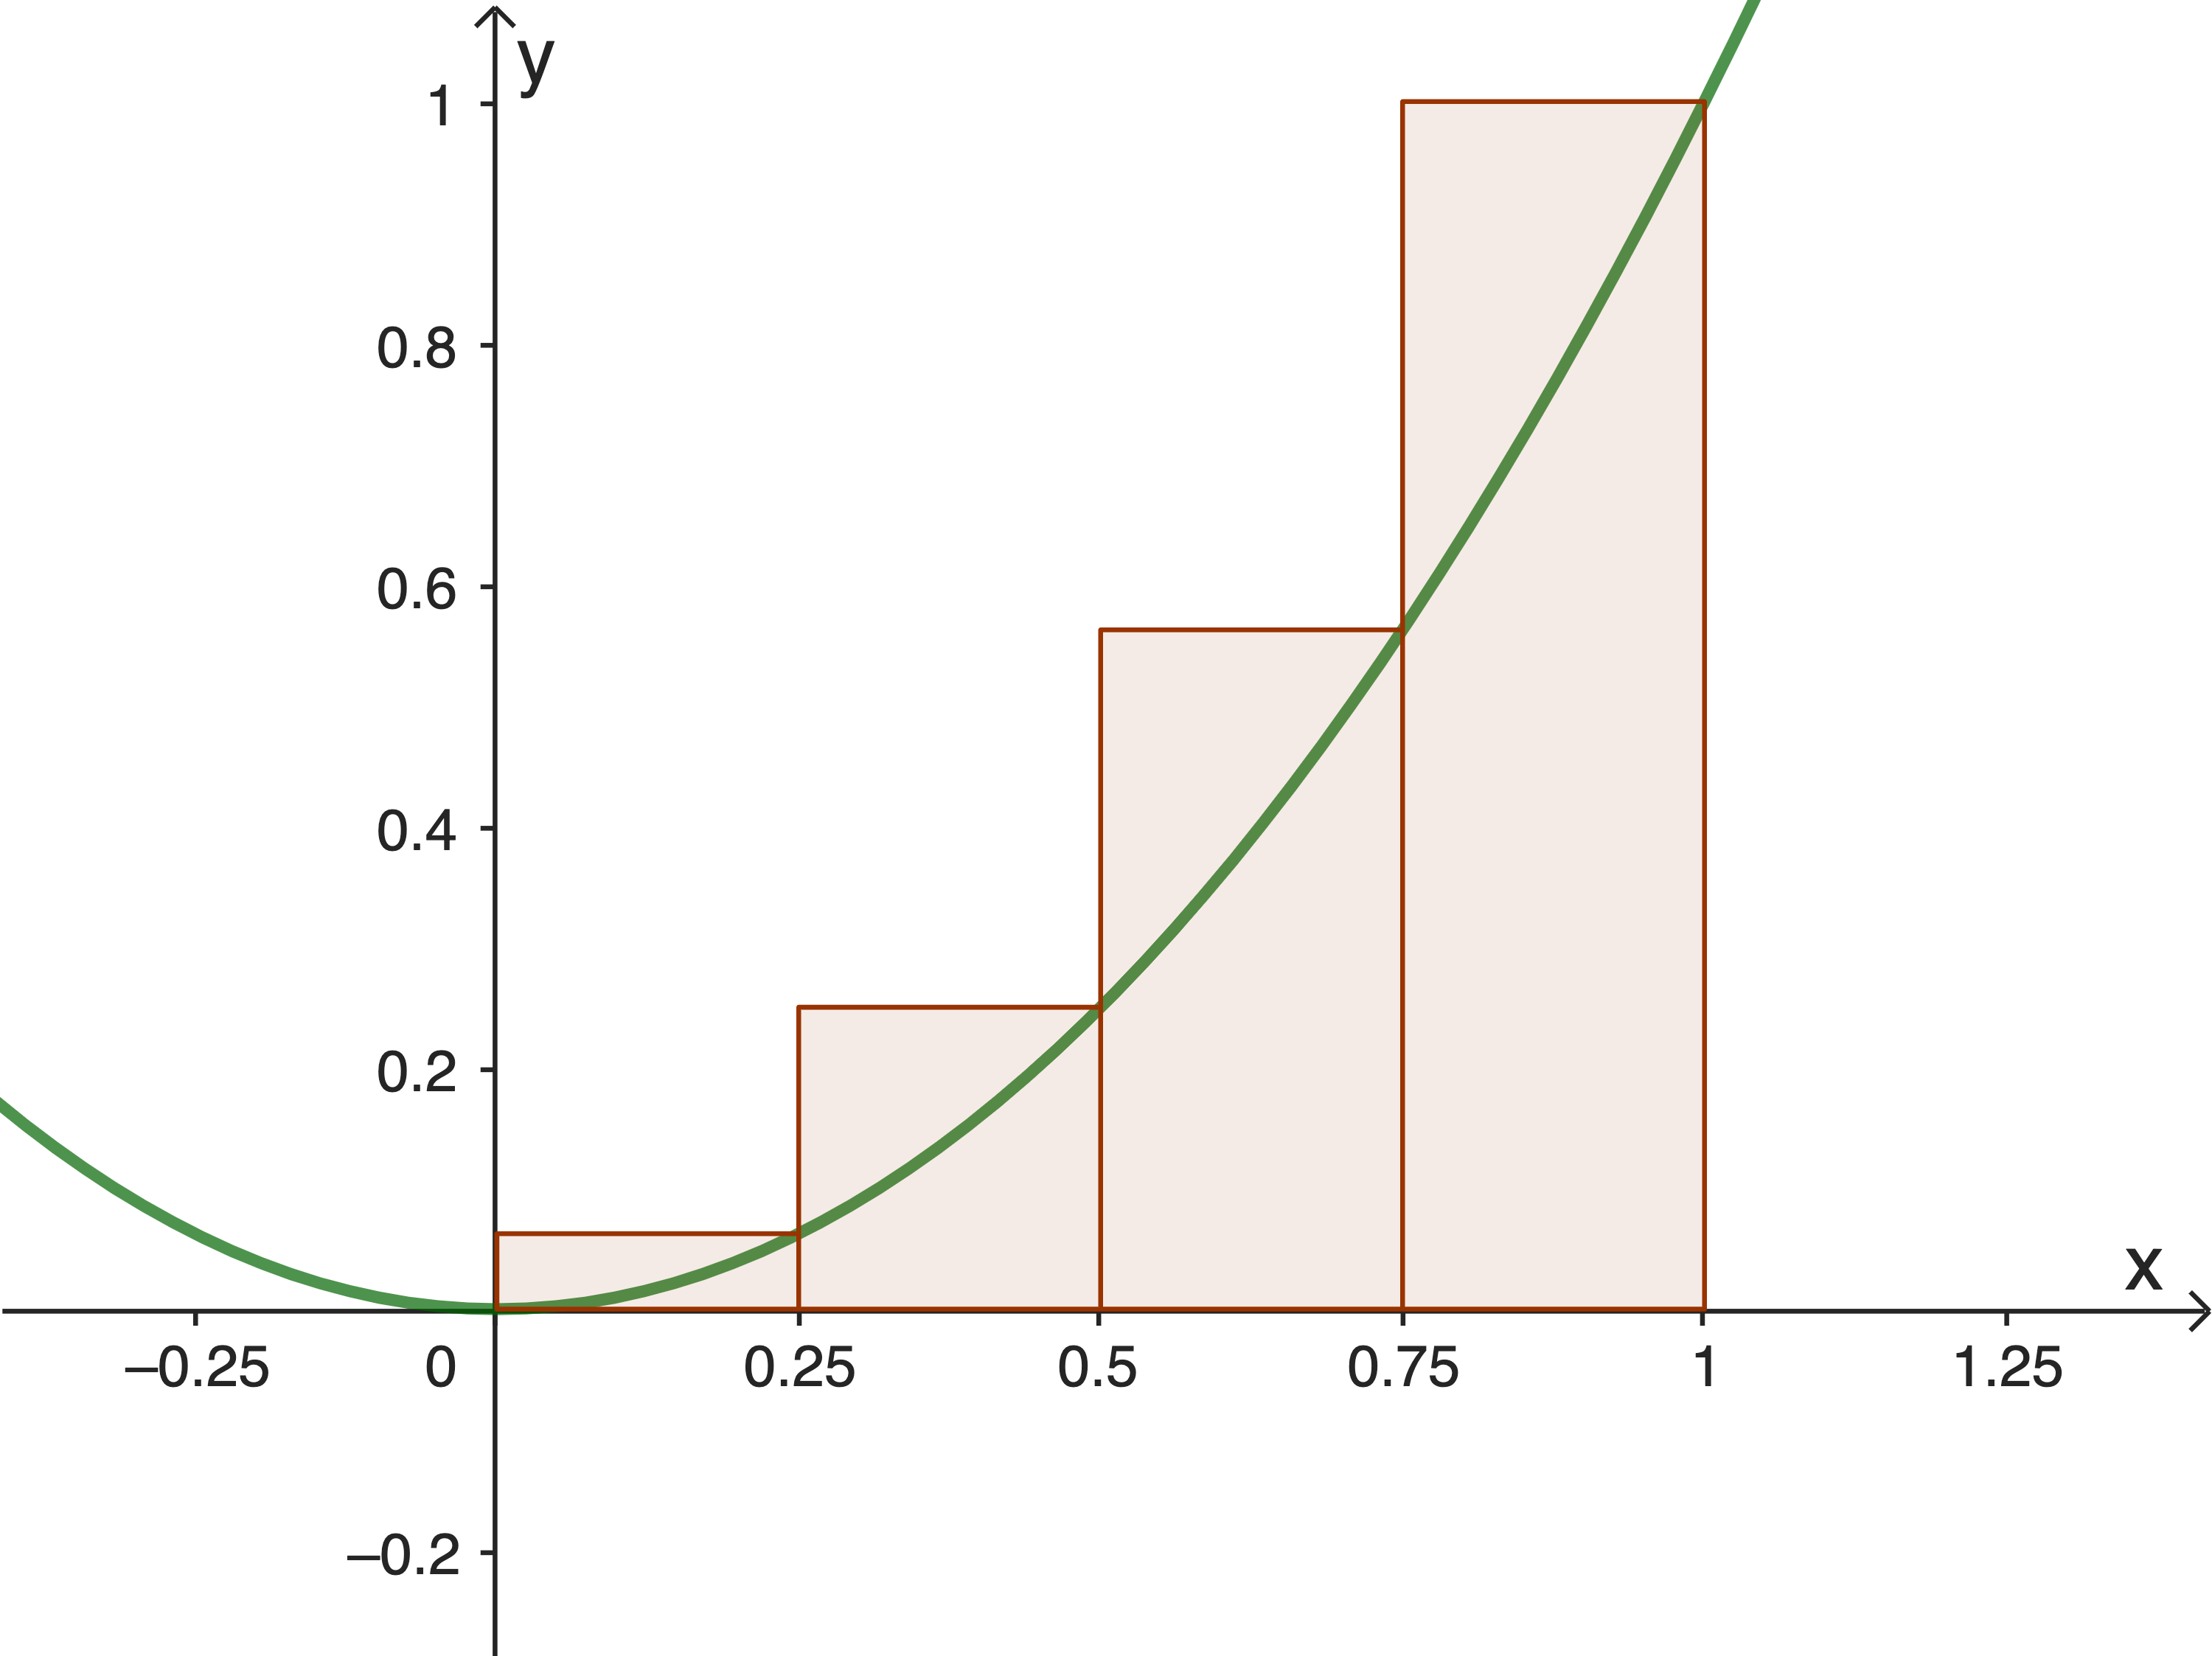
\includegraphics[width = 0.4\textwidth]{media/obersummex-quadrat.png}
\end{center}
Die Summe der Flächeninhalte der 4 Rechtecke in der Figur links nennen wir \textbf{Untersumme} $U_4$.(Beachten Sie, dass es ganz links ein \glqq Rechteck\grqq{} mit der Höhe 0 gibt). Die Summe der Flächeninhalte der 4 Rechtecke in der Figur rechts nennen wir \textbf{Obersumme} $O_4$. Der gesuchte Flächenihalt liegt also irgendwo zwischen $U_4$ und $O_4$. Je mehr Rechtecke wir verwenden, desto besser werden die Näherungen für den Flächeninhalt.

\clearpage
\begin{LA}
	{Die Fläche unter der Quadratfunktion - Teil 1}{FlächeUnterxQuadrat-teil1}
	\begin{enumerate}
		\item 	Zu den Figuren oben:
		      \begin{enumerate}
			      \item Berechnen Sie die beiden Näherungen $U_4$ und $O_4$. \\
			            (Kontrolle: $U_4=\frac{7}{32}$ und $O_4=\frac{15}{32} $)
			      \item Wird das Intervall $[0,1]$ in $8$ Teile zerlegt, erhält man bessere Approximationen (= Näherungen) für den Inhalt der Fläche unter der Parabel. Berechnen Sie $U_8$ und $O_8$.
			            (Kontrolle: $U_8=\frac{35}{128}; \; O_8=\frac{51}{128}$ )
		      \end{enumerate}
		\item Challenges:
		      \begin{enumerate}
			      \item 	Bestimmen Sie je einen Term für die Unter- bzw. Obersumme, wenn man das Intervall in $n$ Teile unterteilt.
			      \item 	Für jedes Zahl $k\in \N$ gilt
			            $$ 1+4+9+16+ \cdots +k^2=\frac{k(k+1)(2k+1)}{6}.$$
			            Verwenden Sie diese Formel, um die Ober- und Untersumme weiter zu vereinfachen.
			      \item Welchen Grenzwert erhält man für die beiden Summen, für $n \rightarrow \infty$?.
		      \end{enumerate}

	\end{enumerate}
\end{LA}

\clearpage

Mit dem Grenzwert von Ober- und Untersumme haben wir eine Methode gefunden, mit der man den Flächeninhalt von beliebigen Gebieten unter der Quadratfunktion berechnen kann.

\begin{center}
	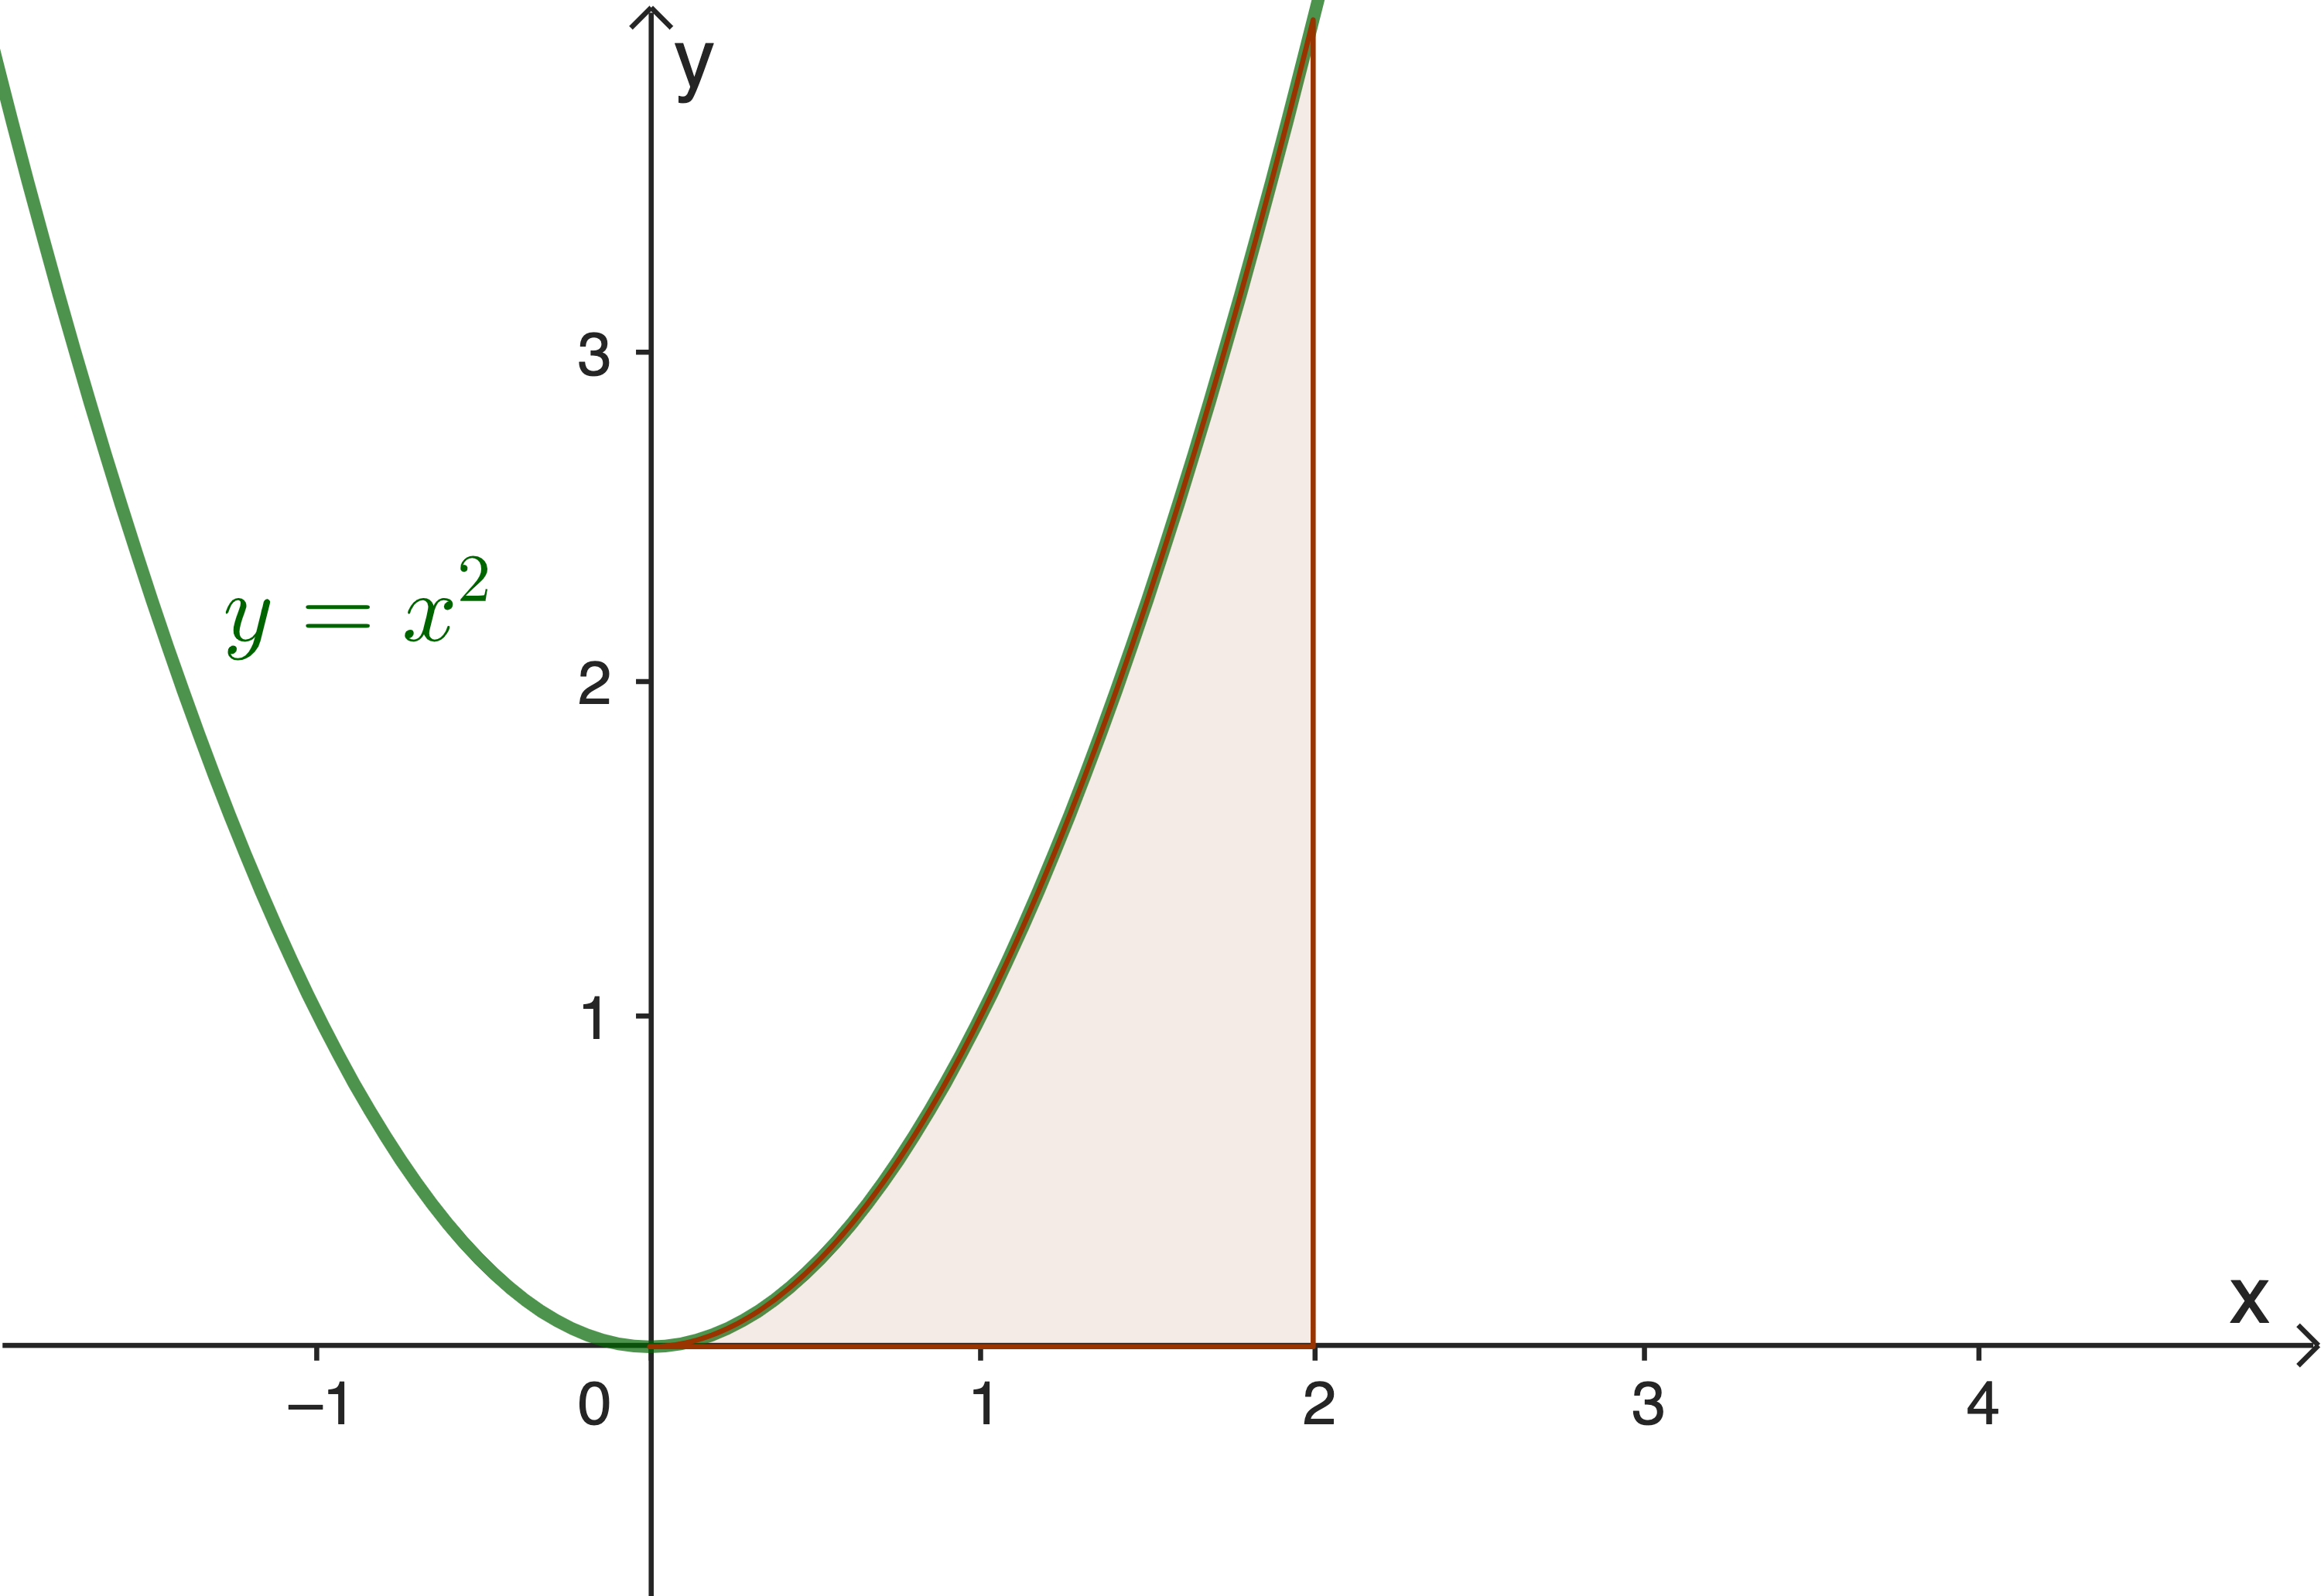
\includegraphics[width = 0.25\textwidth]{media/integral0-2-xquadrat.png}
	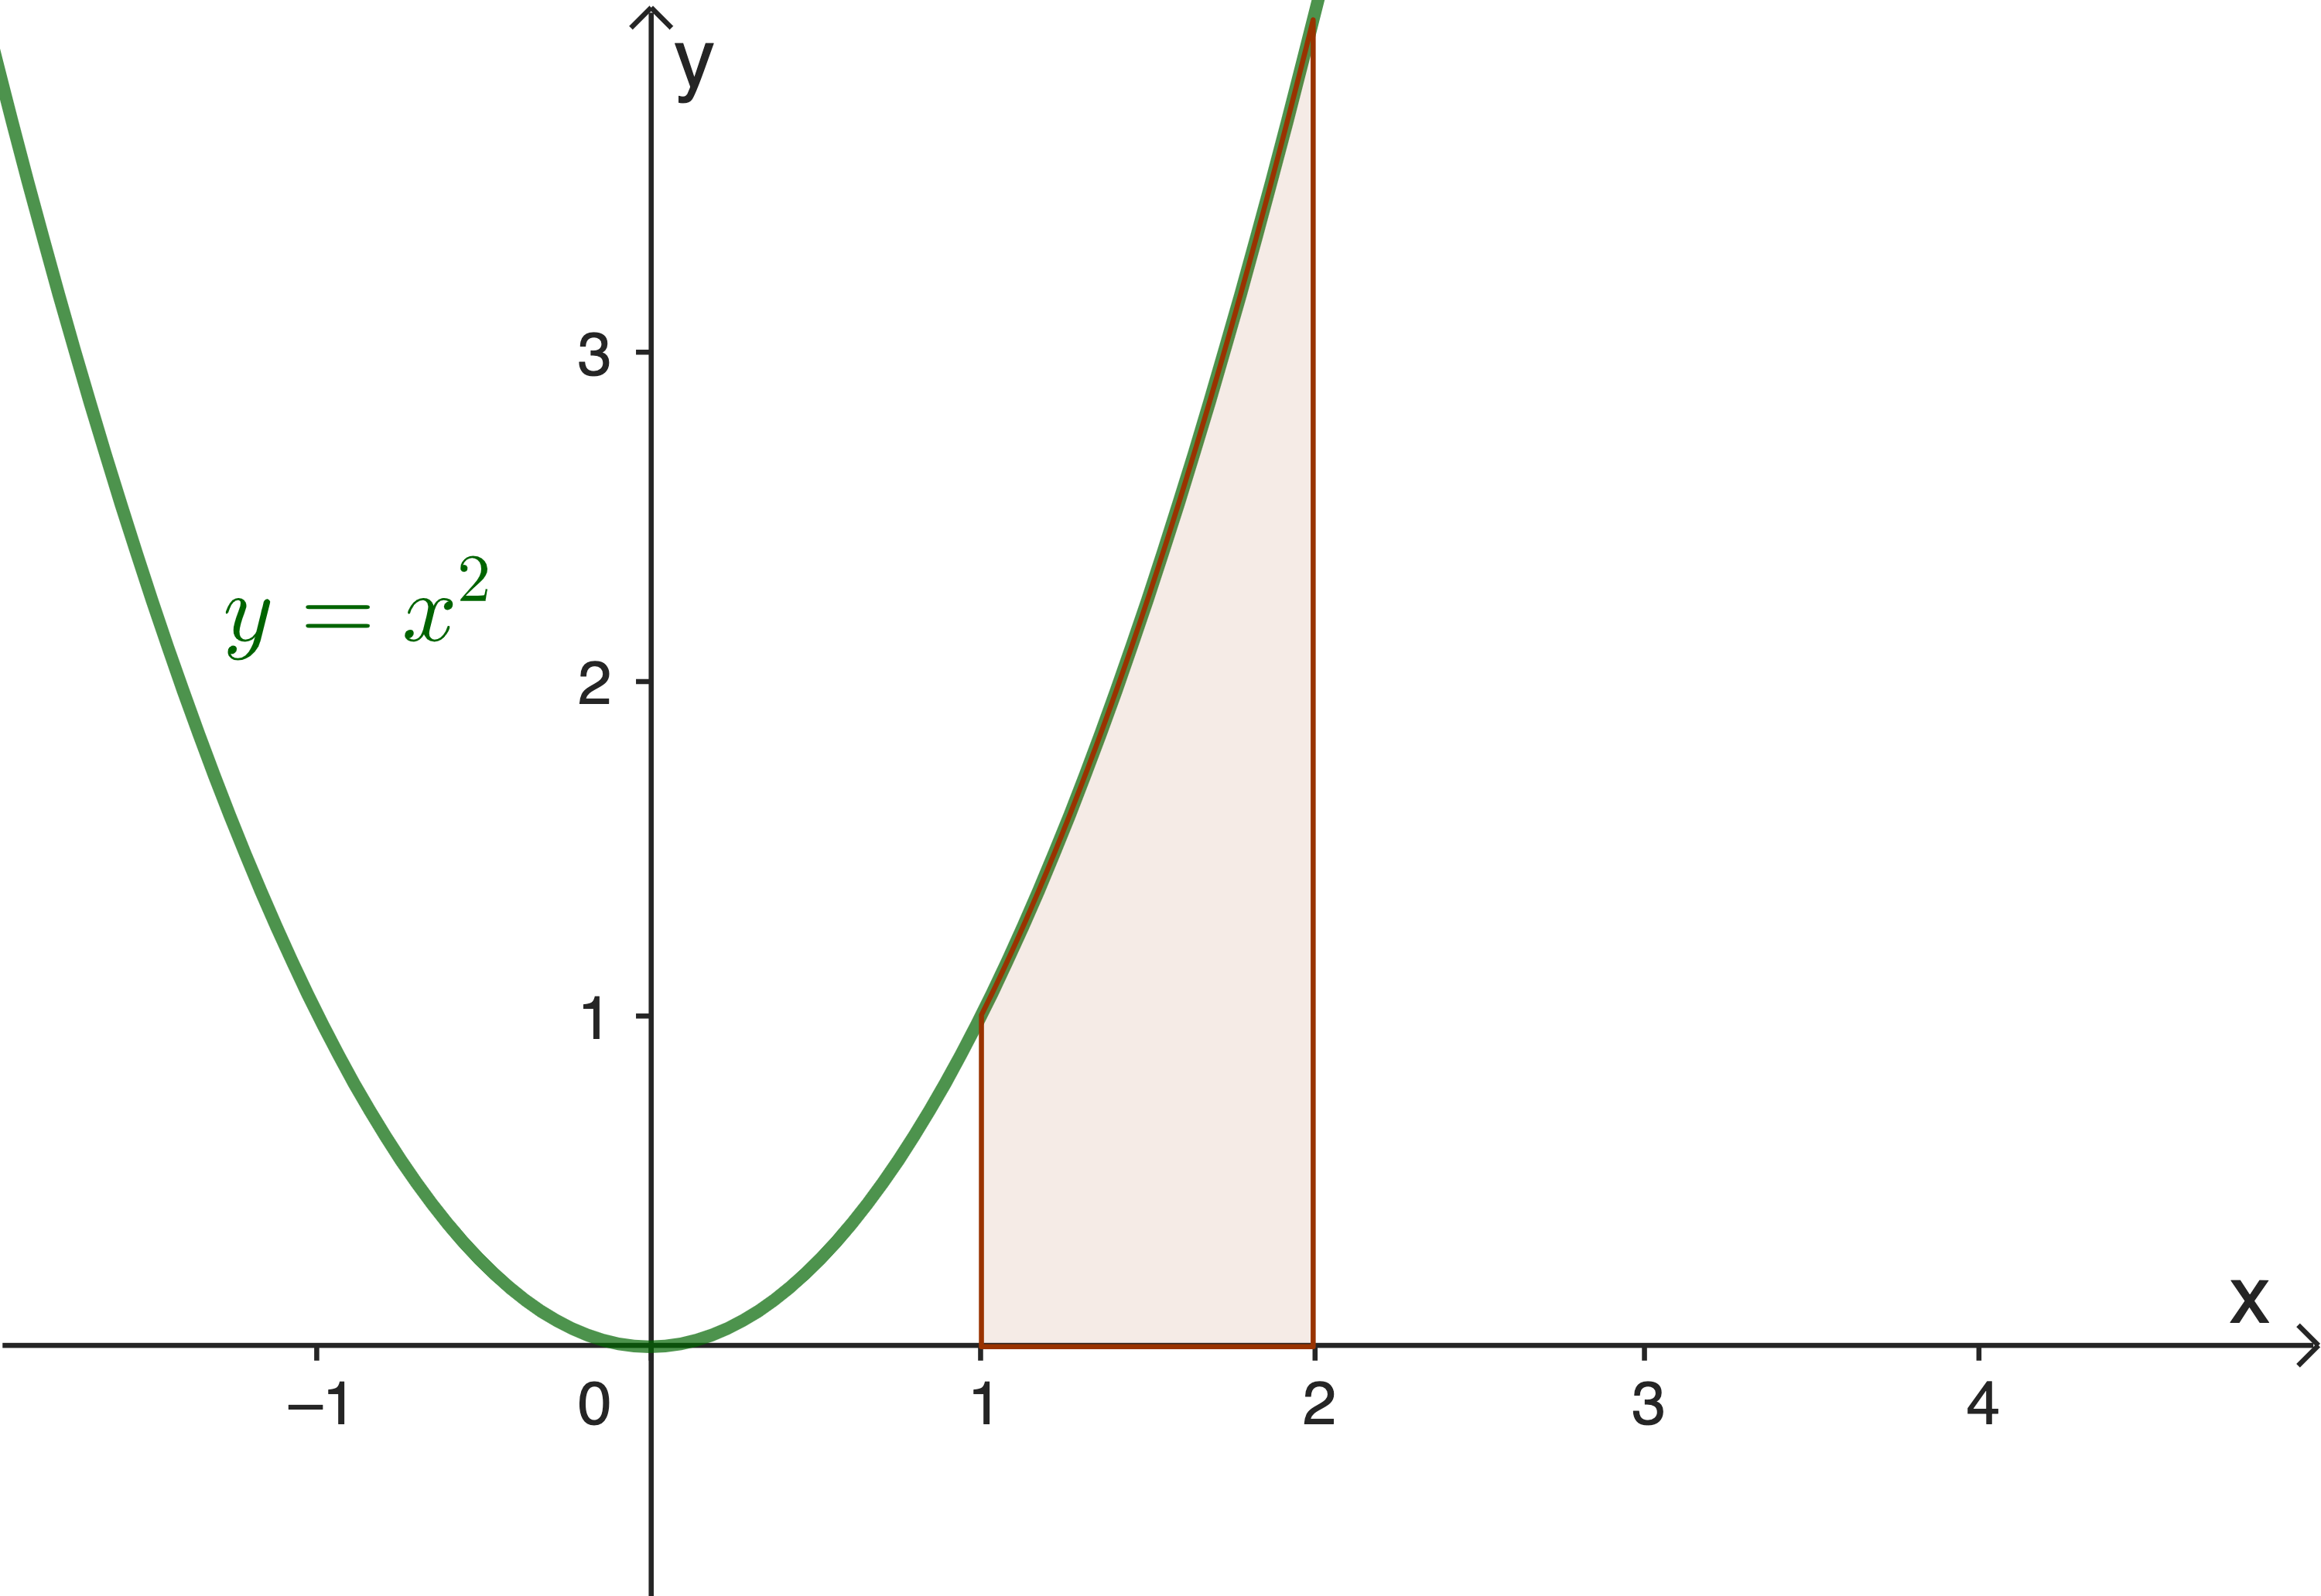
\includegraphics[width = 0.25\textwidth]{media/integral1-2-xquadrat.png}
	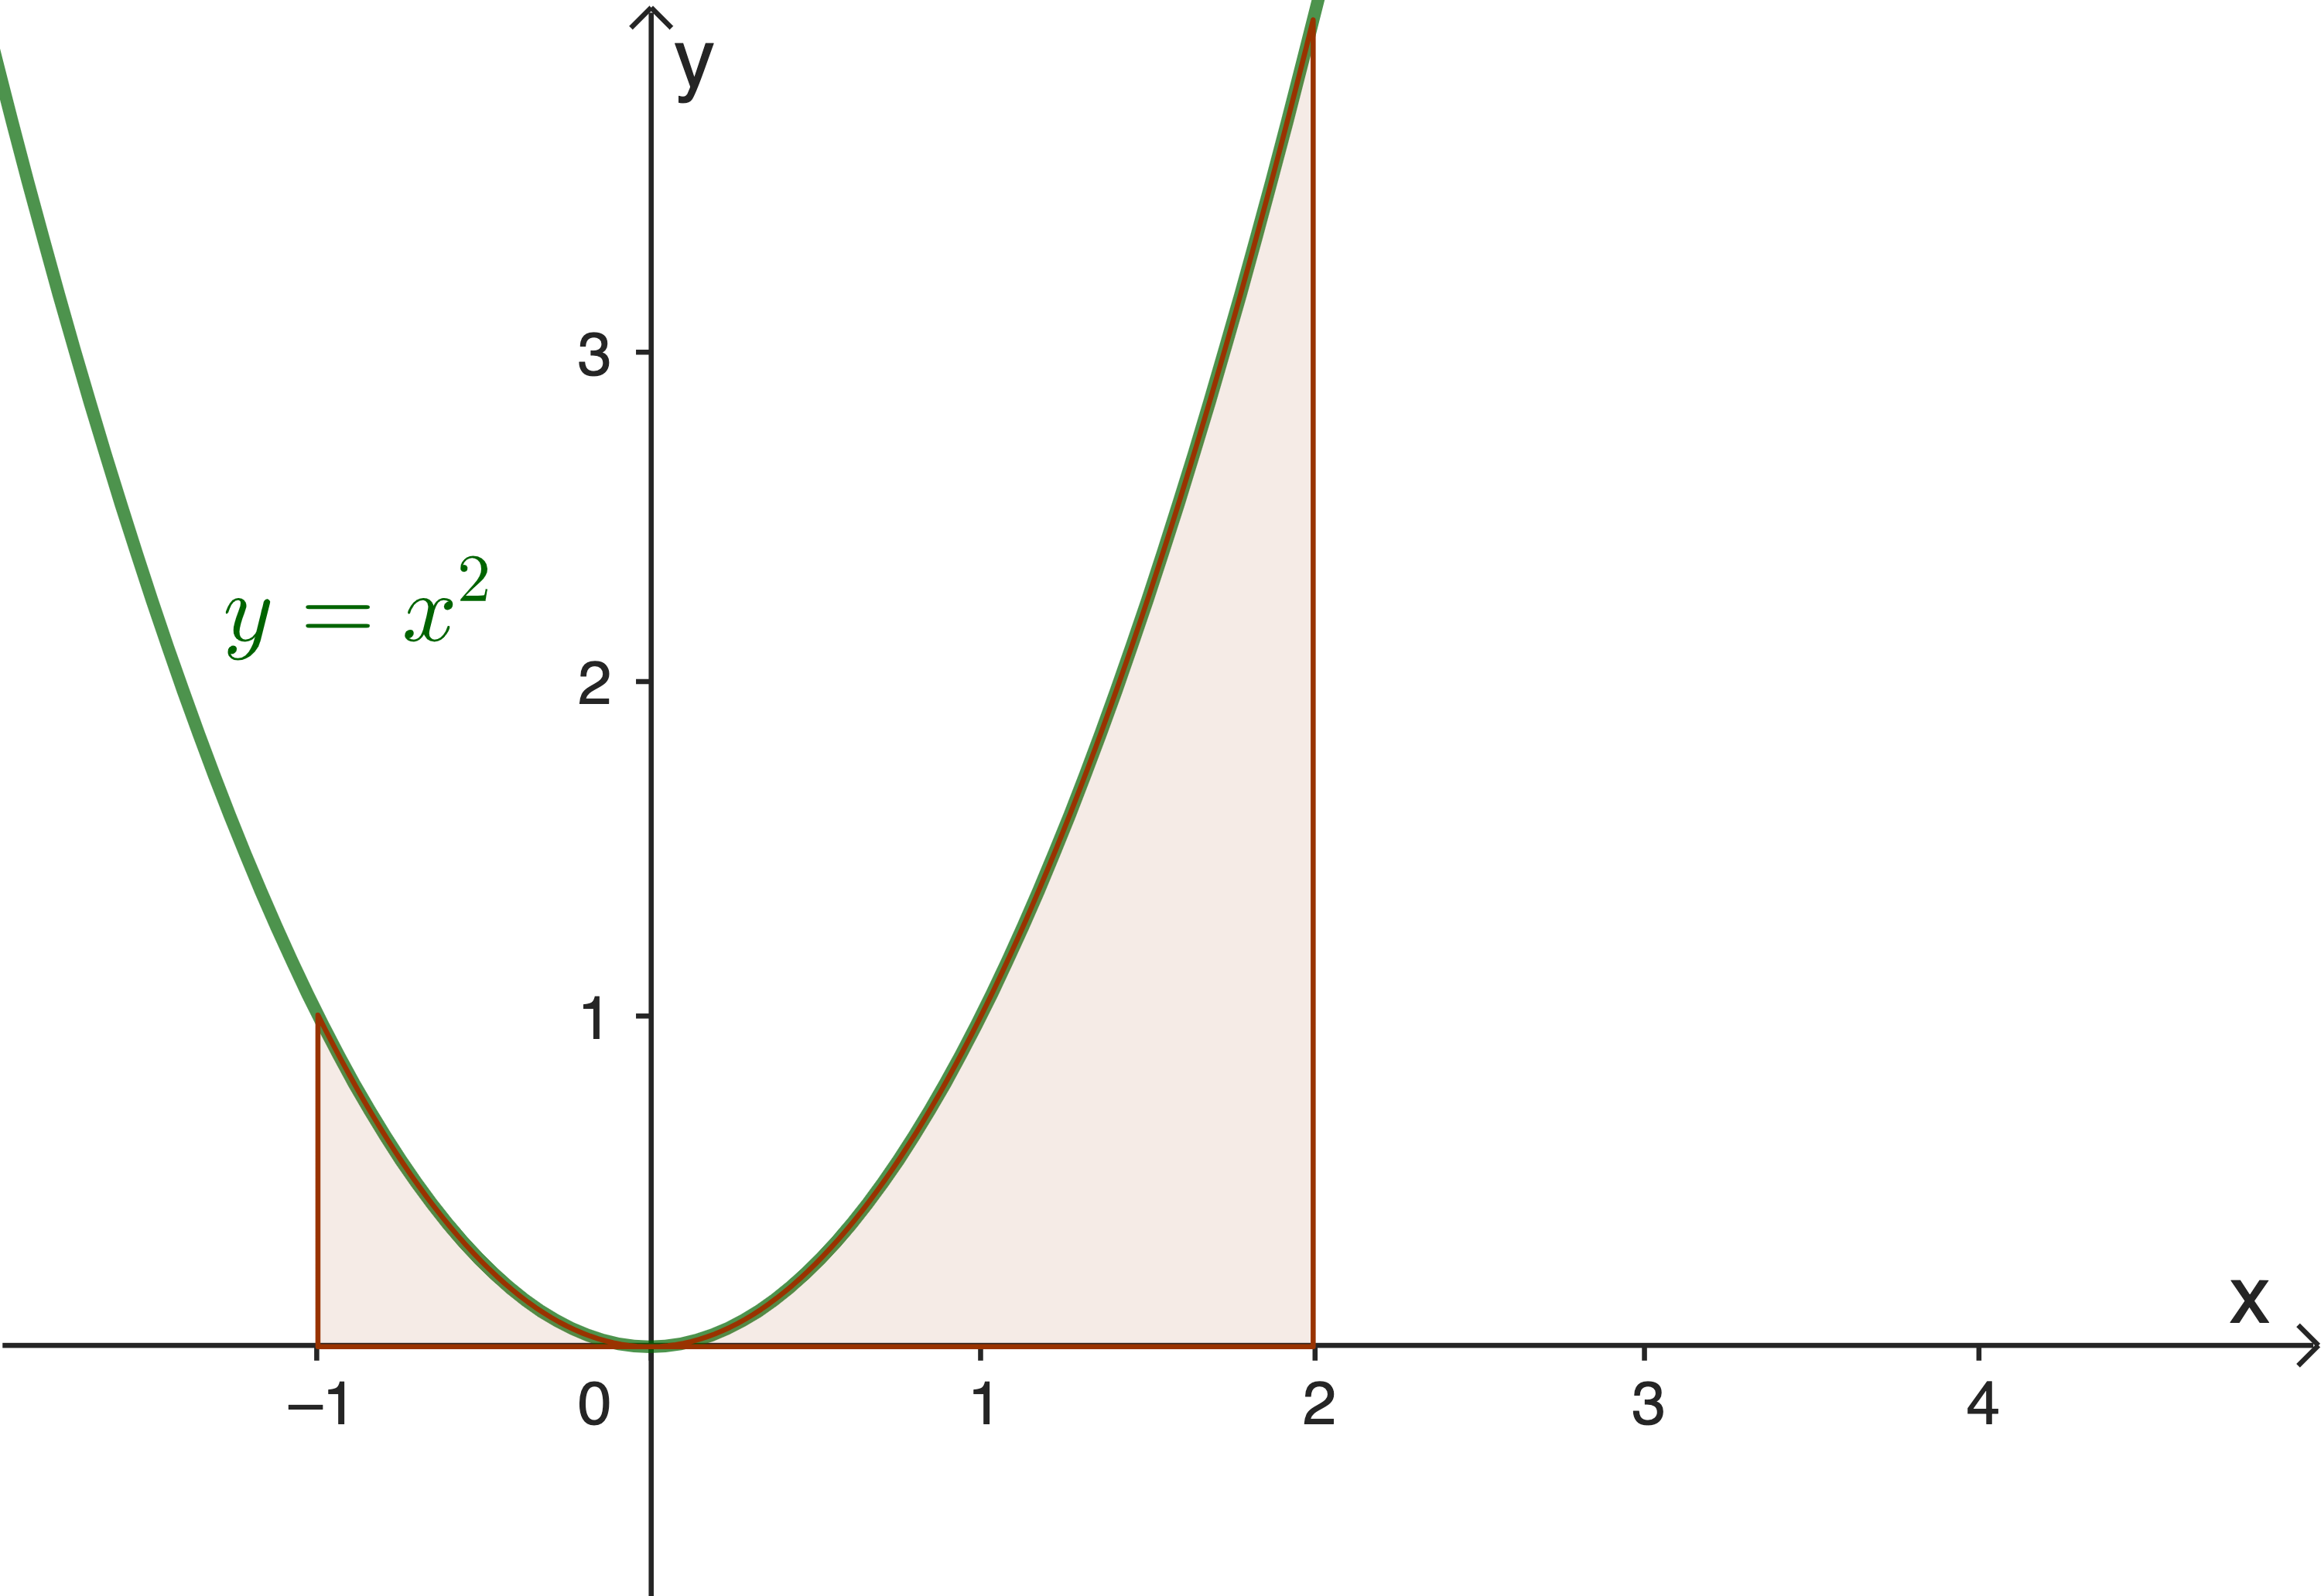
\includegraphics[width = 0.25\textwidth]{media/integral--1-2-xquadrat.png}
\end{center}

Freilich wäre jede dieser Rechnung mit Aufwand verbunden. Einfacher geht es, wenn man das rechte Ende des Intervalls variabel lässt.

Betrachten Sie die Fläche unter dem Graphen von $f(x)=x^2$ im Intervall $[0,b]$:
\begin{center}
	\includegraphics[width=0.5\textwidth]{media/flächeUnterxQuadrat.png}
\end{center}

In der folgenden Lernaufgabe werden wir eine Funktion $F(b)$ herleigen, die in Abhängigkeit von $b$ den Inhalte der Fläche unter der Parabel $y=x^2$ im Intervall $[0, b]$ berechnet. (Eine solche Funktion nennt man eine \emph{Integralfunktion} von $f$)


% Idee: Zur Bestimmung des Flächeninhalts unter der Parabel teilen wir das Intervall $[0,b]$ in vier Teile und betrachten zwei Näherungen für den Flächeninhalt:

% Die Summe der Flächeninhalte der 4 Rechtecke in der Figur links nennen wir \textbf{Untersumme} $U_4$.(Beachten Sie, dass es ganz links ein \glqq Rechteck\grqq{} mit der Höhe 0 gibt)
% \begin{center}
% 	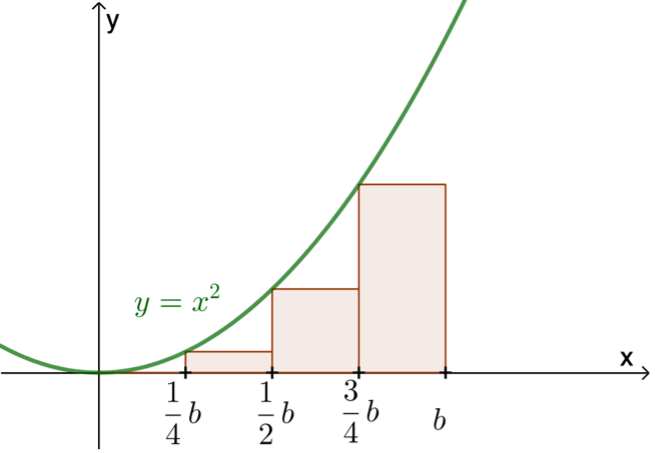
\includegraphics[width=0.5\textwidth]{media/UntersummexQuadrat.png}
% \end{center}

% Die Summe der Flächeninhalte der 4 Rechtecke in der Figur rechts nennen wir \textbf{Obersumme} $O_4$.

% \begin{center}
% 	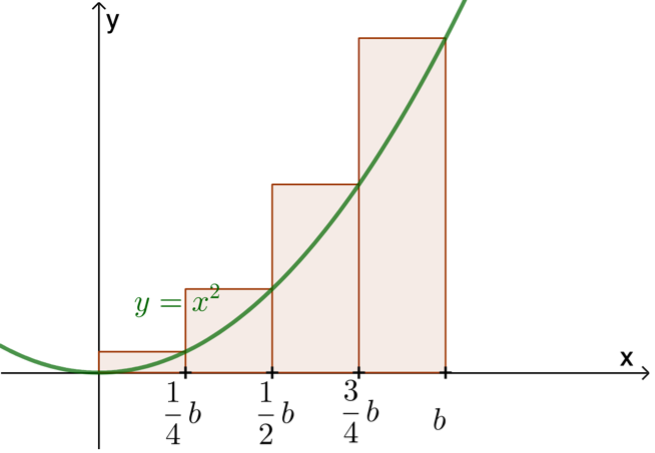
\includegraphics[width=0.5\textwidth]{media/ObersummexQuadrat.png}
% \end{center}
\begin{LA}
	{Die Fläche unter der Quadratfunktion - Teil 2}{FlächeUnterxQuadrat-teil2}
	\begin{enumerate}
		\item Gehen Sie wie in \Cref{LA:FlächeUnterxQuadrat-teil1} vor, um die Fläche unter der Parabel $y=x^2$ im Intervall $[0,b]$ zu berechnen. Berechnen Sie also die Untersumme $U_n$ und die Obersumme $O_n$ für eine Zerlegung des Intervalls in $n$ Teile. Verwenden Sie die Summenformel, um die Terme zu vereinfachen und bestimmen Sie den Grenzwert von $U_n$ und $O_n$ für $n\rightarrow \infty$.
		\item Berechnen Sie mit der Formel die Fläche unter der Parabel $y=x^2$ in den Intervallen $[0,2]$, [1,2] und $[-1,2]$ (Siehe die drei Abbildungen oben).

	\end{enumerate}
\end{LA}































\clearpage
\subsubsection{Ober- und Untersummen}

\begin{satz}
	{Erkenntnis aus der Lernaufgabe}{}
	Der Inhalt der Fläche zwischen der Parabel $y=x^2$ und der $x$-Achse im Intervall $[0,b]$ beträgt
	$$ A=\frac{1}{3} b^3$$
	\begin{center}
		\includegraphics[width=0.5\textwidth]{media/flächeUnterxQuadrat.png}
	\end{center}
\end{satz}


\begin{proof}
	Teilt man das Intervall $[0,b]$ in $n$ Teilintervalle erhält man die Untersumme
	\begin{align*}
		U_n & = \frac{b}{n} \left[f\left(\frac{b}{n} \right)+f\left(\frac{2b}{n} \right)+f\left(\frac{3b}{n} \right)+\cdots +f\left(\frac{(n-1)b}{n} \right)\right] \\
		    & =\frac{b}{n} \left[ \frac{b^2}{n^2} +\frac{4b^2}{n^2} + \frac{9b^2}{n^2} + \cdots +\frac{(n-1)^2 b^2}{n^2} \right]                                    \\
		    & = \frac{b^3}{n^3} \left[1+4+9+\cdots+(n-1)^2 \right]
	\end{align*}

	Analog für die Obersumme:
	$$ O_n=\frac{b^3}{n^3}  [1+4+9+\cdots +n^2 ]$$
	Nun verwenden wir die Formel für die Summe der Quadratzahlen.
	$$ 1+4+9+16+\cdots +k^2=\frac{k(k+1)(2k+1)}{6} $$
	Damit folgt für $k=n-1$:
	$$ U_n= \frac{b^3}{n^3} \left[ \frac{(n-1)n(2n-1)}{6} \right] =  \frac{b^3}{6} \cdot  \frac{2n^2-3n+1}{n^2} = \frac{b^3}{6} \left(2-\frac{3}{n}+\frac{1}{n^2}\right)
	$$
	Und für $k=n$:
	$$ O_n= \frac{b^3}{n^3} \left[ \frac{n(n+1)(2n+1)}{6} \right] =  \frac{b^3}{6} \cdot \frac{2n^2+3n+1}{n^2} = \frac{b^3}{6} \left(2+\frac{3}{n}+\frac{1}{n^2}\right)
	$$
	Der Grenzwert von Ober- und Untersumme beträgt schliesslich:
	$$ \lim_{n\rightarrow\infty} U_n = \lim_{n\rightarrow\infty} O_n = \frac{b^3}{6}\cdot 2 = \frac{b^3}{3}  $$
\end{proof}

% \begin{ueb}{}{}
%     \begin{enumerate}
%         \item  Benutzen Sie die Formel für die Fläche unter der Parabel, um folgende Flächeninhalte zu berechnen.
%         \begin{enumerate}
%             \item Fläche zwischen der $x$-Achse und dem Graphen von $f(x)=x^2$ zwischen $x=0$ und $x=5$.
%             \item Fläche zwischen der $x$-Achse und dem Graphen von $f(x)=x^2$ zwischen $x=3$ und $x=6$.
%             \item Fläche zwischen der $x$-Achse und dem Graphen von $f(x)=x^2+3$ zwischen $x=0$ und $x=2$. Tipp: machen Sie eine Skizze und unterteilen Sie die Fläche in zwei Teile, deren Inhalt Sie berechnen können.
%             \item Fläche zwischen der $x$-Achse und dem Graphen von $f(x)=5\cdot x^2$ zwischen $x=0$ und $x=6$. Tipp: Wie verändern sich die Rechtecke in Unter- und Obersumme, wenn man anstatt $y=x^2$ die Kurve $y=5x^2$ betrachten?
%         \end{enumerate}
%     \item Lösen Sie die Aufgaben auf Seite 124 - 128 im Buch. Beispielsweise 34, 36 und 39.
%     \end{enumerate}
%   
%\end{ueb}

Das Verfahren, das wir für die Funktion $y=x^2$ verwendet haben, lässt sich auch auf andere Funktionen übertragen.
\begin{definition}
	{Ober- und Untersumme}{}
	Sei $f$ eine stetige Funktion $f:\,   [a,b]\rightarrow \R$. Wir unterteilen das Intervall $[a,b]$ in $n$ gleich grosse Teilintervalle $[x_{k-1} x_{k}]$ der Breite $ \Delta x = \frac{b-a}{n}$.
	\bigskip



	\textbf{Untersumme $U_n$:} \\
	\begin{center}
		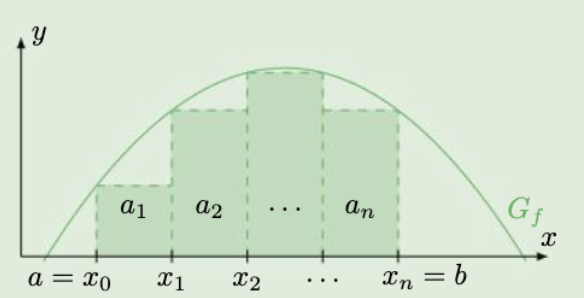
\includegraphics[width = 0.3\textwidth]{media/UntersummeDef.png}
	\end{center}
	Für jedes Teilintervall wählen wir den kleinsten Funktionswert $\underline{f_k}$.
	%$\underline{f_k} = \min \{ f(x) | x\in [x_{k-1}, x_{k}] \}$
	Die Untersumme $U_n$ ist definiert als die Summe der Flächeninhalte $a_k = \Delta x \cdot \underline{f_k}$ der Rechtecke mit der Breite $\Delta x$ und der Höhe $\underline{f_k}$:
	$$U_n = a_1 +  a_2 + \cdots +a_n = \sum_{k=1}^n \underline{f_k} \cdot \Delta x $$


	\bigskip

	\textbf{Obersumme $O_n$:} \\
	\begin{center}
		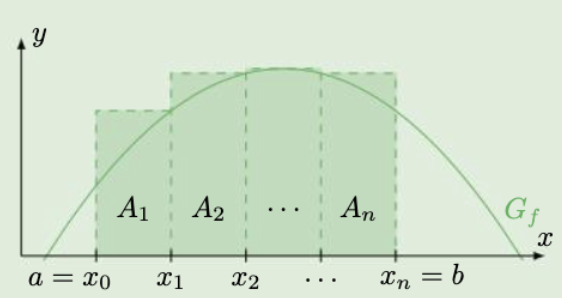
\includegraphics[width = 0.3\textwidth]{media/ObersummeDef.png}
	\end{center}
	Für jedes Teilintervall wählen wir den grössten Funktionswert $\overline{f_k}$.
	%$\underline{f_k} = \max \{ f(x) | x\in [x_{k-1}, x_{k}] \}$
	Die Obersumme $O_n$ ist definiert als die Summe der Flächeninhalte $a_k = \Delta x \cdot \overline{f_k}$ der Rechtecke mit der Breite $\Delta x$ und der Höhe $\overline{f_k}$:
	$$O_n = A_1 +  A_2 + \cdots +A_n = \sum_{k=1}^n \overline{f_k} \cdot \Delta x $$






	% \begin{center}
	%     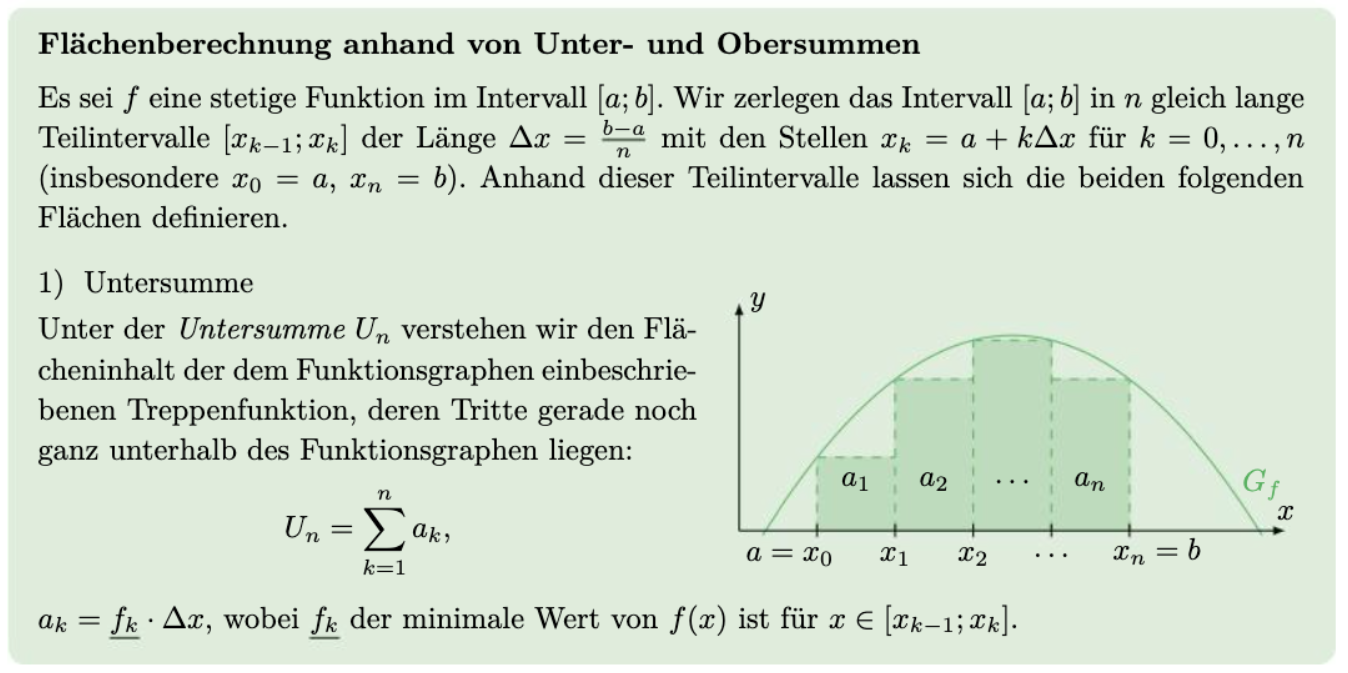
\includegraphics[width = \textwidth]{media/defUntersumme.png}

	%     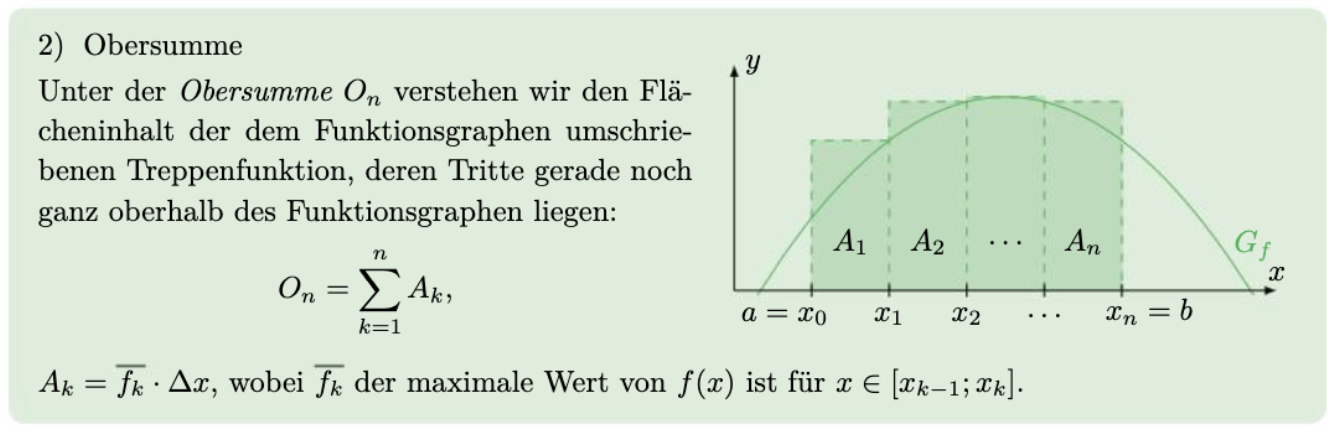
\includegraphics[width = \textwidth]{media/defObersumme.png}
	% \end{center}


\end{definition}

\clearpage
\begin{ueb}
	{Fläche unter einer Funktion dritten Grades}{}


	\begin{enumerate}
		\item Die Abbildung zeigt den Grundriss eines Schwimmbeckens, dessen Breite alle 2m gemessen wurde. Schätzen Sie den Flächeninhalt des Beckens mit Hilfe von Unter- und Obersummen ab.
		      \begin{center}
			      \includegraphics[width = 0.3\textwidth]{media/SchwimmbeckenFläche.png}
		      \end{center}


		\item
		      In dieser Aufgabe sollen Sie die Fläche unter dem Graphen der Funktion $f(x) = \frac{1}{100} x^3$ im Intervall $[0,10]$ untersuchen.
		      Tipp: Der Taschenrechner TI 30 X Pro kann mit Summenzeichen umgehen. Siehe dieses \href{https://youtu.be/rxhaYyTZ25o}{Anleitungsvideo}.

		      \begin{enumerate}
			      \item Berechnen Sie die Untersumme $U_5$ und die Obersumme $O_5$.
			      \item Berechnen Sie die Untersumme $U_{10}$ und die Obersumme $O_{10}$.
			      \item Bestimmen Sie je einen Term für die Unter- bzw. Obersumme $U_n$ bzw. $O_n$, wenn man das Intervall in $n$ Teile unterteilt.
			            Dazu können Sie die Formel für die Summe der Kubikzahlen verwenden:
			            $$ 1^3 + 2^3 + 3^3 + \cdots + k^3 = \left( \frac{k(k+1)}{2} \right)^2 $$
			      \item Welchen Grenzwert erhält man für die beiden Summen, für $n \rightarrow \infty$?
		      \end{enumerate}
	\end{enumerate}
\end{ueb}


\clearpage
\emph{Lösungen:}
\begin{enumerate}
	\item Schwimmbecken:

	      Untersumme $U = 55 m^2$; \quad Obersumme $O = 83.8 m^2$. Die echte Fläche liegt also zwischen diesen beiden Werten.
	\item Fläche unter kubischer Funktion
	      \begin{enumerate}
		      \item $U_5= 16,\quad O_5 = 36$
		      \item $U_{10} = 20.25,\quad O_{10} = 30.25$
		      \item $U_n = 25\left(1-\frac{1}{n}\right)^2; \quad O_n = 25\left(1+\frac{1}{n}\right)^2$
		      \item $\lim_{n\rightarrow\infty} U_n = \lim_{n\rightarrow\infty} O_n = 25$
	      \end{enumerate}

\end{enumerate}

\newpage












\subsubsection{Das bestimmte Integral und Integralfunktionen}


\begin{definition}
	{Das bestimmte Integral}{}
	% 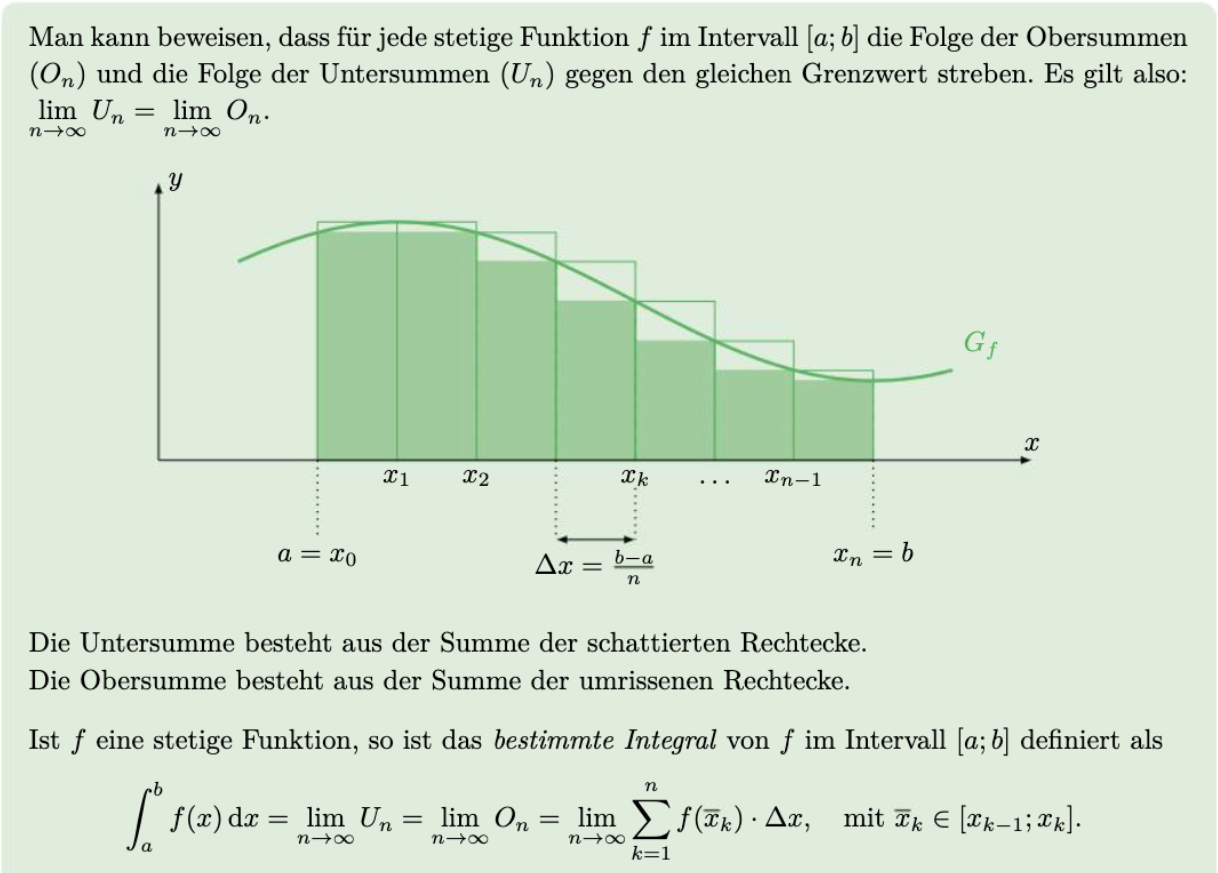
\includegraphics[width = \textwidth]{media/defBestInt-1.png}
	% 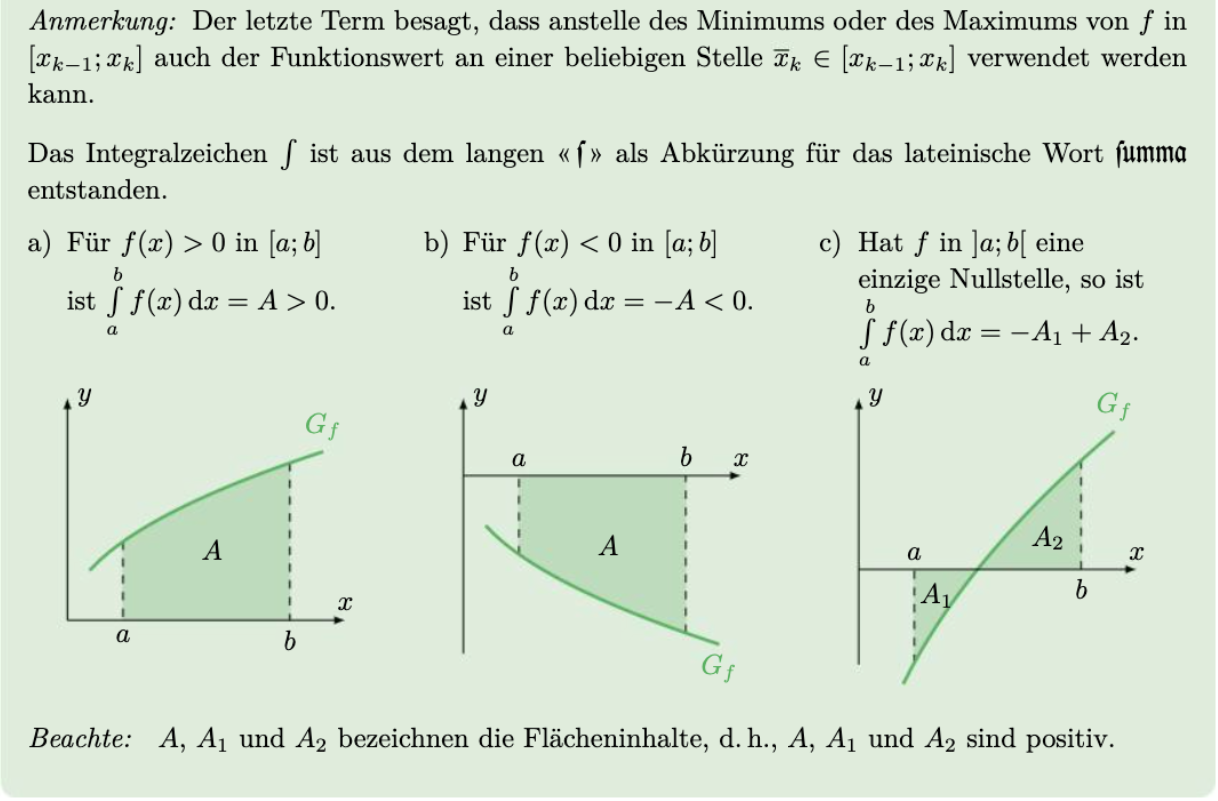
\includegraphics[width = \textwidth]{media/defBestInt-2.png}
	Sei $f$ eine Funktion $f:\,   [a,b]\rightarrow \R$. Falls Unter- und Obersumme den gleichen Grenzwert besitzen $\lim_{n\rightarrow\infty} U_n = \lim_{n\rightarrow\infty} O_n$, so sagt man, die Funktion $f$ sei \emph{integrierbar}. Den gemeinsamen Grenzwert von Ober- und Untersumme nennt man das \emph{bestimmte Integral der Funktion $f$ von $a$ nach $b$}.

	Schreibweise
	$$ \int_a^b f(x) dx =  \lim_{n\rightarrow\infty} U_n = \lim_{n\rightarrow\infty} O_n$$

	Wenn die Funktion $f$ im Intervall $[a,b]$ nicht negativ ist, entspricht das bestimmte Integral dem Flächeninhalt des Gebietes, das durch den Graphen von $f$, die $x$-Achse und die Geraden $x=a$ und $x=b$ berandet wird. Weil aber die Flächeninhalte der Rechtecke in Ober- und Untersumme berechnet werden mit $a_= \Delta x \cdot \underline{f_k}$ bzw. $A_k = \Delta x \cdot \overline{f_k}$, kann das bestimmte Integral auch negative Werte annehmen, wenn die Funktion im Intervall negative Funktionswerte annimmt.
	\begin{center}
		\includegraphics[width = \textwidth]{media/flächenbilanz.png}
	\end{center}




\end{definition}


\begin{bsp}
	{}{}
	In der Lernaufgabe am Anfang des Kapitels haben wir gezeigt, dass der Inhalt der Fläche zwischen der Parabel $y=x^2$ und der $x$-Achse im Intervall $[0,b]$  $ A=\frac{1}{3} b^3$ beträgt. In anderen Worten:
	$$ \int_0^b x^2 dx = \frac{1}{3} b^3$$
	Mit dieser Formel können wir nun verschiedene bestimmte Integrale berechnen:
	\begin{itemize}
		\item $\int_0^5 x^2 dx = \frac{1}{3} 5^3 = \frac{125}{3}$
		\item $\int_1^3 x^2 dx = \int_0^3 x^2 dx - \int_0^1 x^2 dx = \frac{1}{3} 3^3 -\frac{1}{3} 1^3 = \frac{26}{3}$
	\end{itemize}
	\begin{center}
		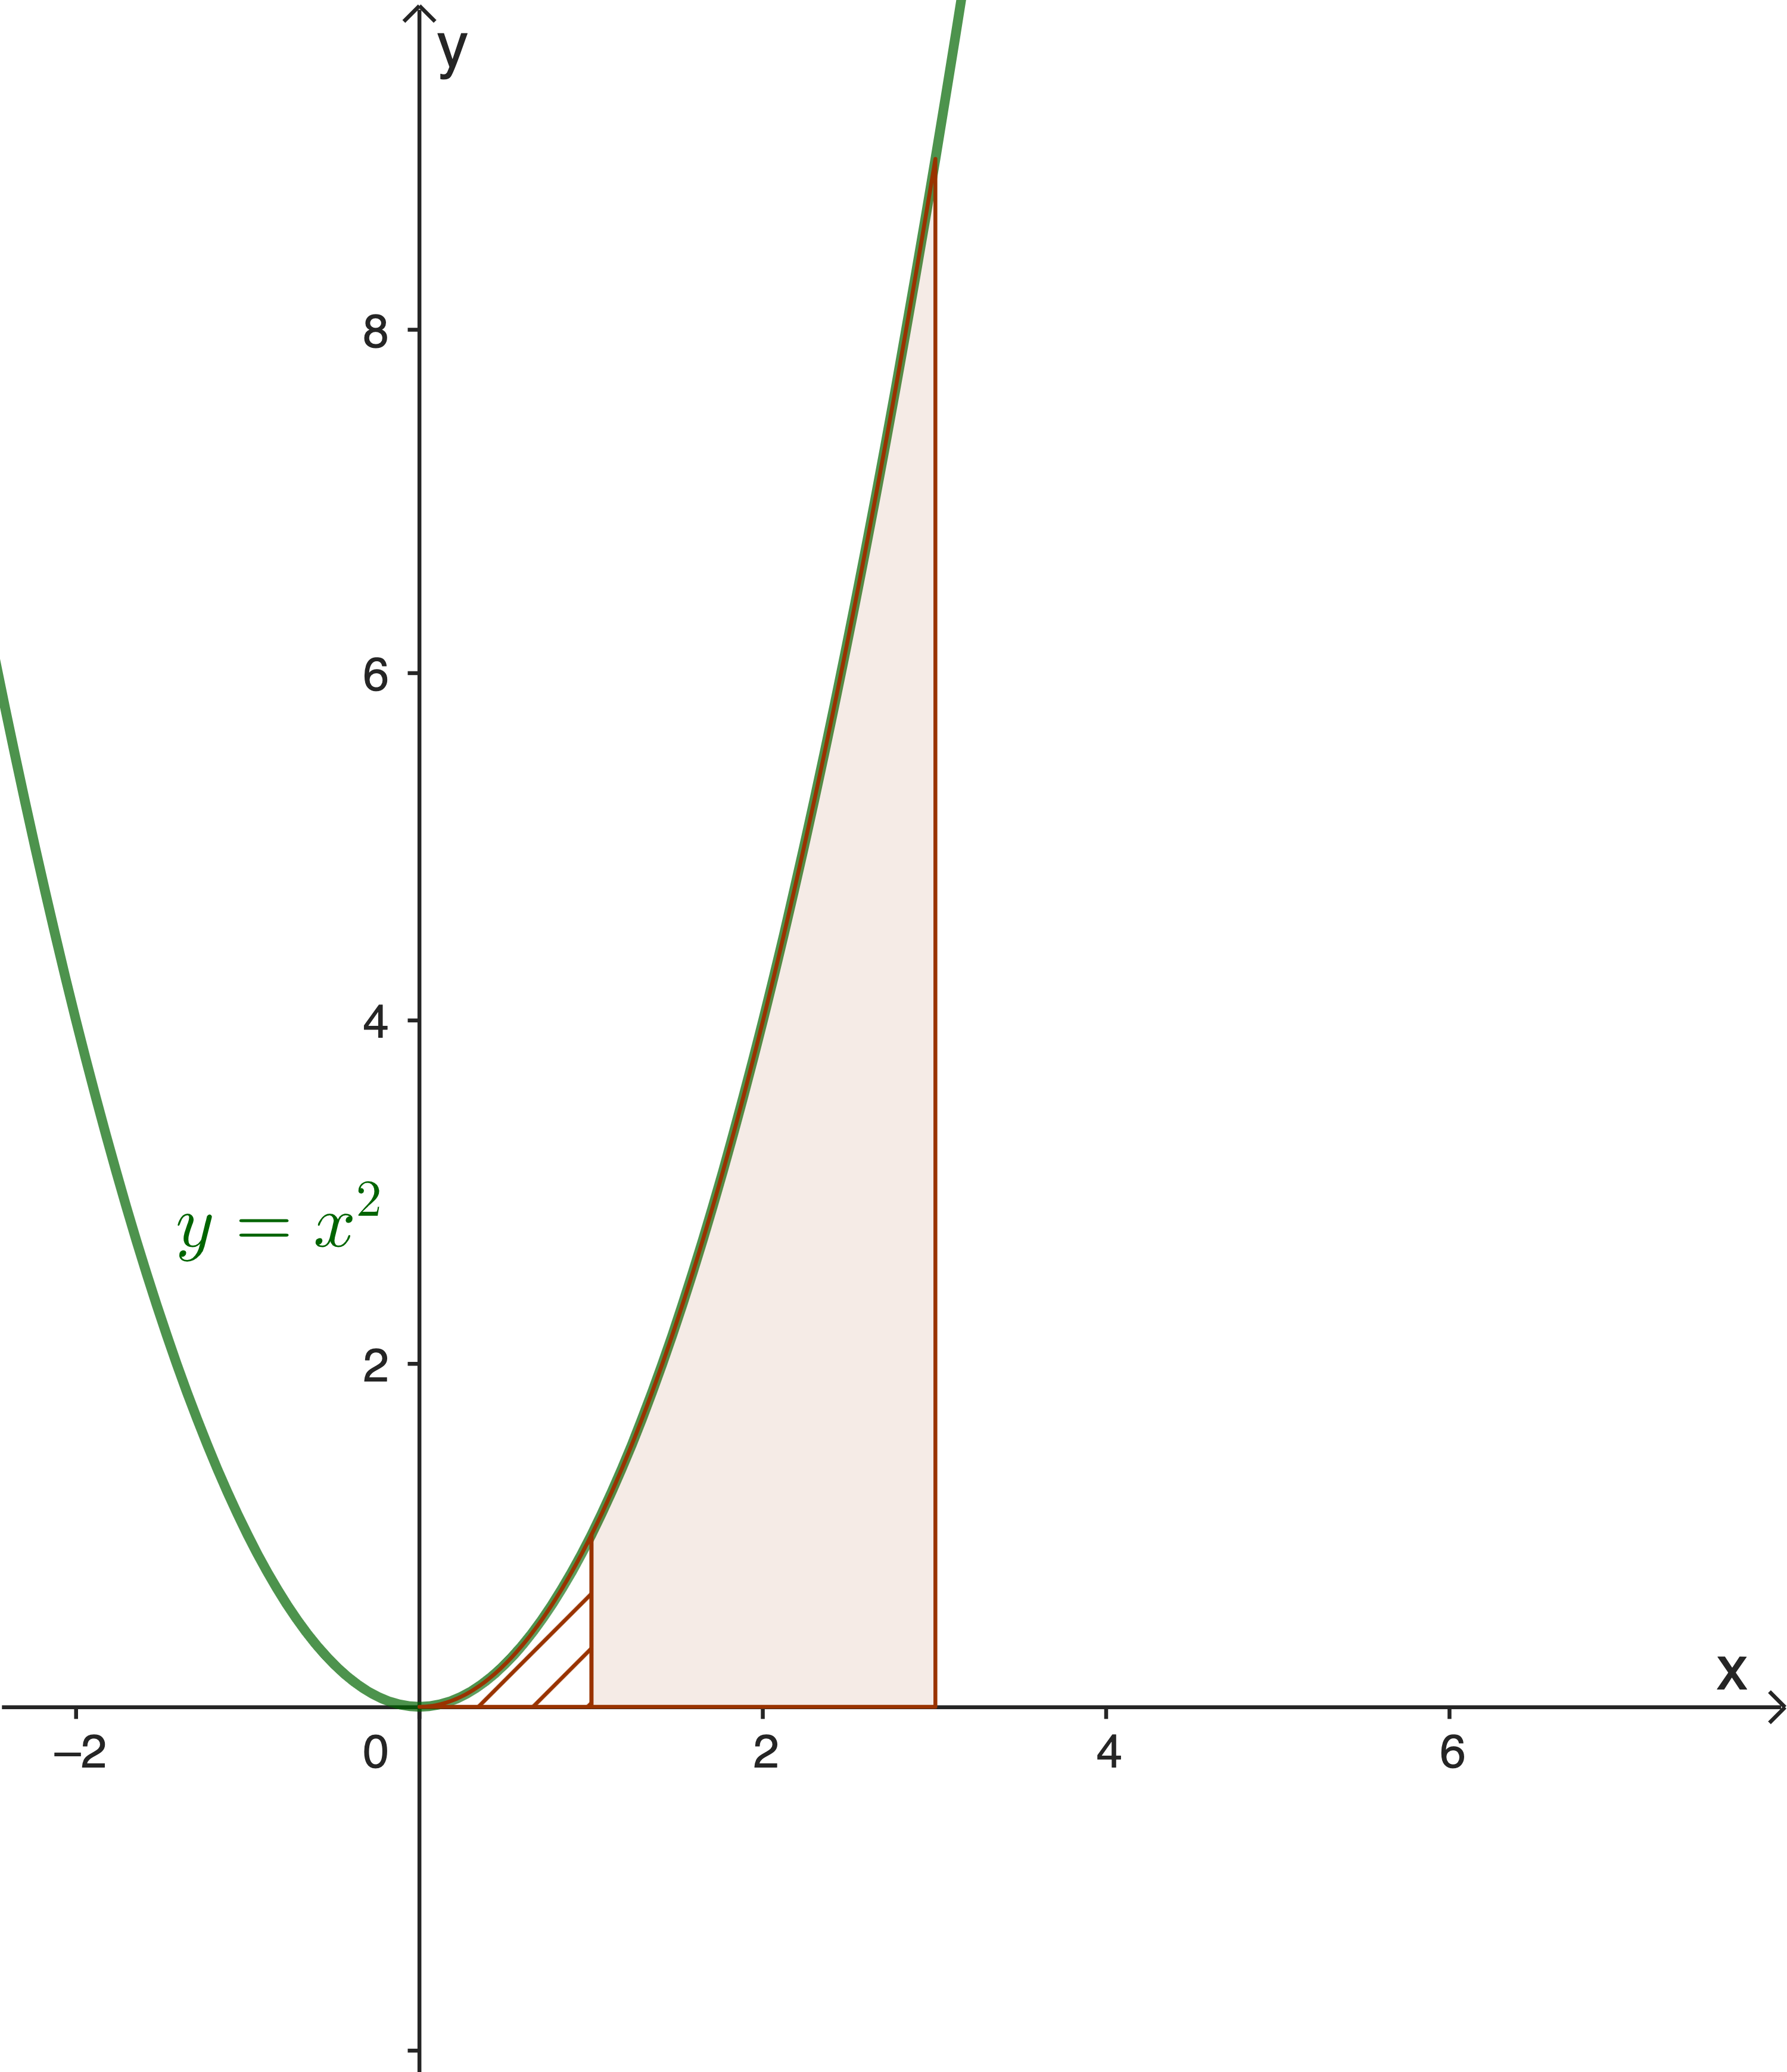
\includegraphics[width = 0.5\textwidth]{media/integral1-3.png}
	\end{center}
\end{bsp}
Beim zweiten Beispiel haben wir intuitiv die erste der folgenden Integrationsregeln verwendet:
\begin{satz}
	{Aufteilen und Vertauschen der Integrationsgrenzen }{}
	$$\int_a^b f(x) dx + \int_b^c f(x) dx = \int_a^c f(x) dx $$
	$$\int_b^a f(x) dx  = - \int_a^b f(x) dx $$
\end{satz}
Um die zweite Regel zu verstehen, muss man einen Blick zurück auf die Definition der Untersummen werfen:
$$U_n = \sum_{k=1}^n \underline{f_k} \cdot \Delta x, $$
wobei $\Delta x = \frac{b-a}{n}$ die Breite der Rechtecke ist.

Wenn die beiden Integrationsgrenzen vertauscht werden, ändert sich in der ganzen Summe bloss das Vorzeichen im Zähler von $\Delta x$.

In der Lernaufgabe am Anfang des Kapitels haben wir die Formel $$ \int_0^b x^2 dx = \frac{1}{3}b^3$$ hergeleitet. Weil wir die obere Grenze des Integrals variabel gelassen haben, kann man mit dieser Formel in Kombination mit dem Aufteilen der Integrationsgrenzen alle bestimmte Integrale rund um die Funktion $f(x)=x^2$ berechnen. So gilt zum Beispiel:

$$\int_5^{10} x^2 dx = \int_0^{10} x^2 dx - \int_0^5 x^2 dx = \frac{1}{3}10^3-\frac{1}{3}5^3 = \frac{875}{3}$$

Diese Idee lässt sich auf andere Funktionen übertragen:
\begin{definition}{Integralfunktion}{}
	Sei $f$ eine stetige Funktion. Die Integralfunktion von $f$ zur unteren Grenze $a$ ist definiert als:
	$$F_a (b) = \int_a^b f(x) dx$$
\end{definition}
Bemerkung: Die untere Grenze $a$ des Integrals ist hier fest gewählt, während die obere Grenze $b$ variabel ist.
\begin{bsp}
	{Integralfunktion der Quadratfunktion zur unteren Grenze $0$}{}
	Sei $f(x)=x^2$. Die Erkenntnis aus der Lernaufgabe am Anfang des Kapitels lautet dann:
	$$F_0(b)=\frac{1}{3} b^3$$
\end{bsp}
% \clearpage
\begin{ueb}
	{}{}


	\begin{enumerate}
		\item Für die Funktion \(f\) gilt:
		      \[
			      \int_{-1}^{1} f(x)\,dx = -2
			      \quad\text{und}\quad
			      \int_{1}^{4} f(x)\,dx = 5.
		      \]
		      Berechnen Sie die vier Integrale.

		      \begin{enumerate}
			      \item \(\displaystyle \int_{4}^{1} f(x)\,dx\)
			      \item \(\displaystyle \int_{-1}^{4} f(x)\,dx\)
			      \item \(\displaystyle \int_{1}^{1} f(x)\,dx\)
			      \item \(\displaystyle \int_{-1}^{1} 4 \cdot f(x)\,dx\)
		      \end{enumerate}
		\item Der Graph \(G_f\) der Funktion \(f\) ist gegeben.
		      \begin{center}
			      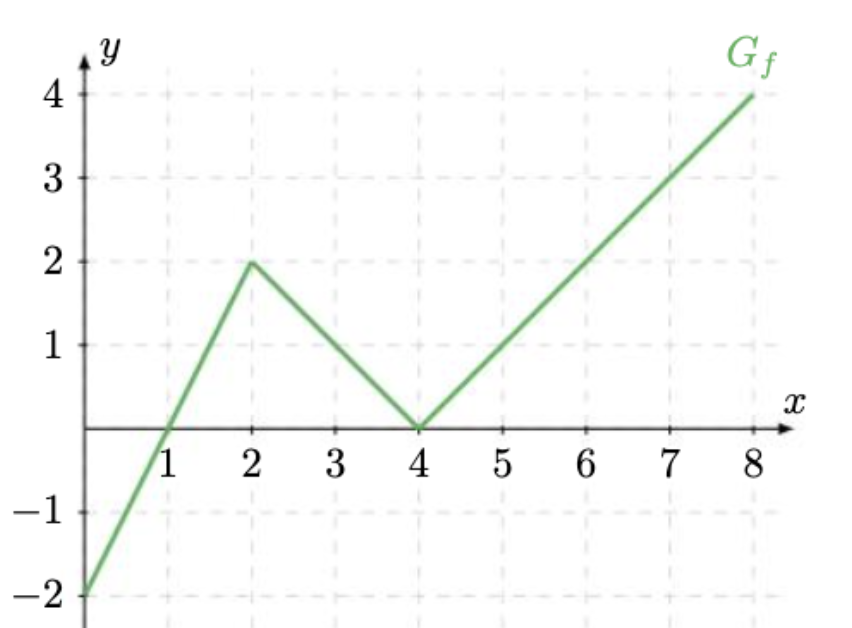
\includegraphics[width = 0.3 \textwidth]{media/GraphAufgabe45.png}
		      \end{center}

		      \begin{enumerate}
			      \item Bestimmen Sie \(\displaystyle \int_{1}^{7} f(x)\,dx.\)
			      \item Bestimmen Sie \(\displaystyle \int_{0}^{1} f(x)\,dx.\)
			      \item Bestimmen Sie \(\displaystyle \int_{0}^{7} f(x)\,dx.\)
			      \item Berechnen Sie den Inhalt der Fläche, die der Graph \(G_f\) im Intervall \([0,7]\) mit der \(x\)-Achse einschliesst.
		      \end{enumerate}

		\item Skizzieren Sie den Graphen der folgenden Funktionen. Markieren Sie in der Skizze die Fläche mit dem Inhalt  \(F_0(b) = \int_0^b f(x) \, dx\) (mit \(b \ge 0\)).

		      Geben Sie anschliessend eine Formel für den Inhalt der markierten Fläche an.

		      %   Bestimme jeweils die Funktionsgleichung der Integralfunktion \(F_0(b) = \int_0^b f(x) \, dx\) (mit \(b \ge 0\)) der folgenden
		      %   Funktion \(f\).

		      %   \textit{Tipp:} Es handelt sich hier immer um lineare Funktionen, weshalb sich die Integralfunktion
		      %   anhand des Funktionsgraphen durch geometrische Überlegungen bestimmen lässt.

		      \begin{enumerate}
			      \item \(f(x) = 1\)
			      \item \(f(x) = 2\)
			      \item \(f(x) = c,\; c \in \mathbb{R}_0^{+}\)
			      \item \(f(x) = x\)
			      \item \(f(x) = 2x\)
			      \item \(f(x) = mx,\; m \in \mathbb{R}_0^{+}\)
			      \item \(f(x) = x + 1\)
			      \item \(f(x) = 2x + 1\)
			      \item \(f(x) = mx + q,\; m,c \in \mathbb{R}_0^{+}\)
		      \end{enumerate}


	\end{enumerate}
\end{ueb}
\clearpage

\emph{Lösungen}

\begin{enumerate}
	\item Integrale Berechnen
	      \begin{enumerate}
		      \item -5
		      \item 3
		      \item 0
		      \item -8
	      \end{enumerate}
	\item Graph
	      \begin{enumerate}
		      \item 7.5
		      \item -1
		      \item 6.5
		      \item 8.5
	      \end{enumerate}
	\item Integralfunktionen
	      \begin{enumerate}
		      \item $F_0(b) = b$
		      \item $F_0(b) = 2b$
		      \item $F_0(b) = c\cdot b$
		      \item $F_0(b) = \frac{1}{2} b^2$
		      \item $F_0(b) = b^2$
		      \item $F_0(b) = \frac{m}{2} b^2$
		      \item $F_0(b) = \frac{1}{2} b^2 + b$
		      \item $F_0(b) = b^2 + b$
		      \item $F_0(b) = \frac{m}{2} b^2 + q\cdot b$
	      \end{enumerate}
\end{enumerate}
\clearpage
\subsection{Der Hauptsatz der Differential- und Integralrechnung}

% In Aufgaben 48 im Buch haben wir mit geometrischen Überlegungen einige Integralfunktionen hergeleitet:
% \begin{itemize}
%     \item $F_0(x) = \int_0^x 1 \,dt = x$
%     \item $F_0(x) = \int_0^x t \,dt = \frac{1}{2}t^2$
%     \item $F_0(x) = \int_0^x (t+1) \,dt = \frac{1}{2}t^2 + t$
%     \item $F_0(x) = \int_0^x 2 \,dt = 2x$
%     \item $F_0(x) = \int_0^x 2t \,dt = t^2$
%     \item $F_0(x) = \int_0^x (2t+1) \,dt = t^2 + t$
% \end{itemize}
% In Aufgabe 49 haben wir einige andere Integralfunktionen als Grenzwerte von Ober- und Untersummen gefunden:
% \begin{itemize}
%     \item $F_0(x) = \int_0^x t^2 \,dt = \frac{1}{3}t^3$
%     \item $F_0(x) = \int_0^x t^3 \,dt = \frac{1}{4}t^4$
%     \item $F_0(x) = \int_0^x t^5 \,dt = \frac{1}{6}t^6$
%     \item $F_0(x) = \int_0^x \left(\frac{1}{2} t^2 +1 \right) \,dt = \frac{1}{6} t^3 +t$
% \end{itemize}

Bestimmte Integrale lassen sich immer als Grenzwerte von Ober- und Untersumme bestimmen. Das Problem ist aber: Diese Berechnung ist aufwendig - insbesondere weil sie für jede neue Funktion und für jedes neue Intervall von vorne begonnen werden muss.

Integralfunktionen lösen einen Teil des Problems: Kennt man von einer Funktion $f$, eine Integralfunktion $F_a(b)=\int_a^b f(x) \,dx$, kann man damit jedes bestimmte Integral von $f$ wie folgt berechnen:
$$ \int_c^d f(x) \,dx = \int_a^d f(x) \,dx - \int_a^c f(x) \,dx =F_a(d) - F_a(c)$$

\begin{figure}[!htb]
	\minipage{0.32\textwidth}
	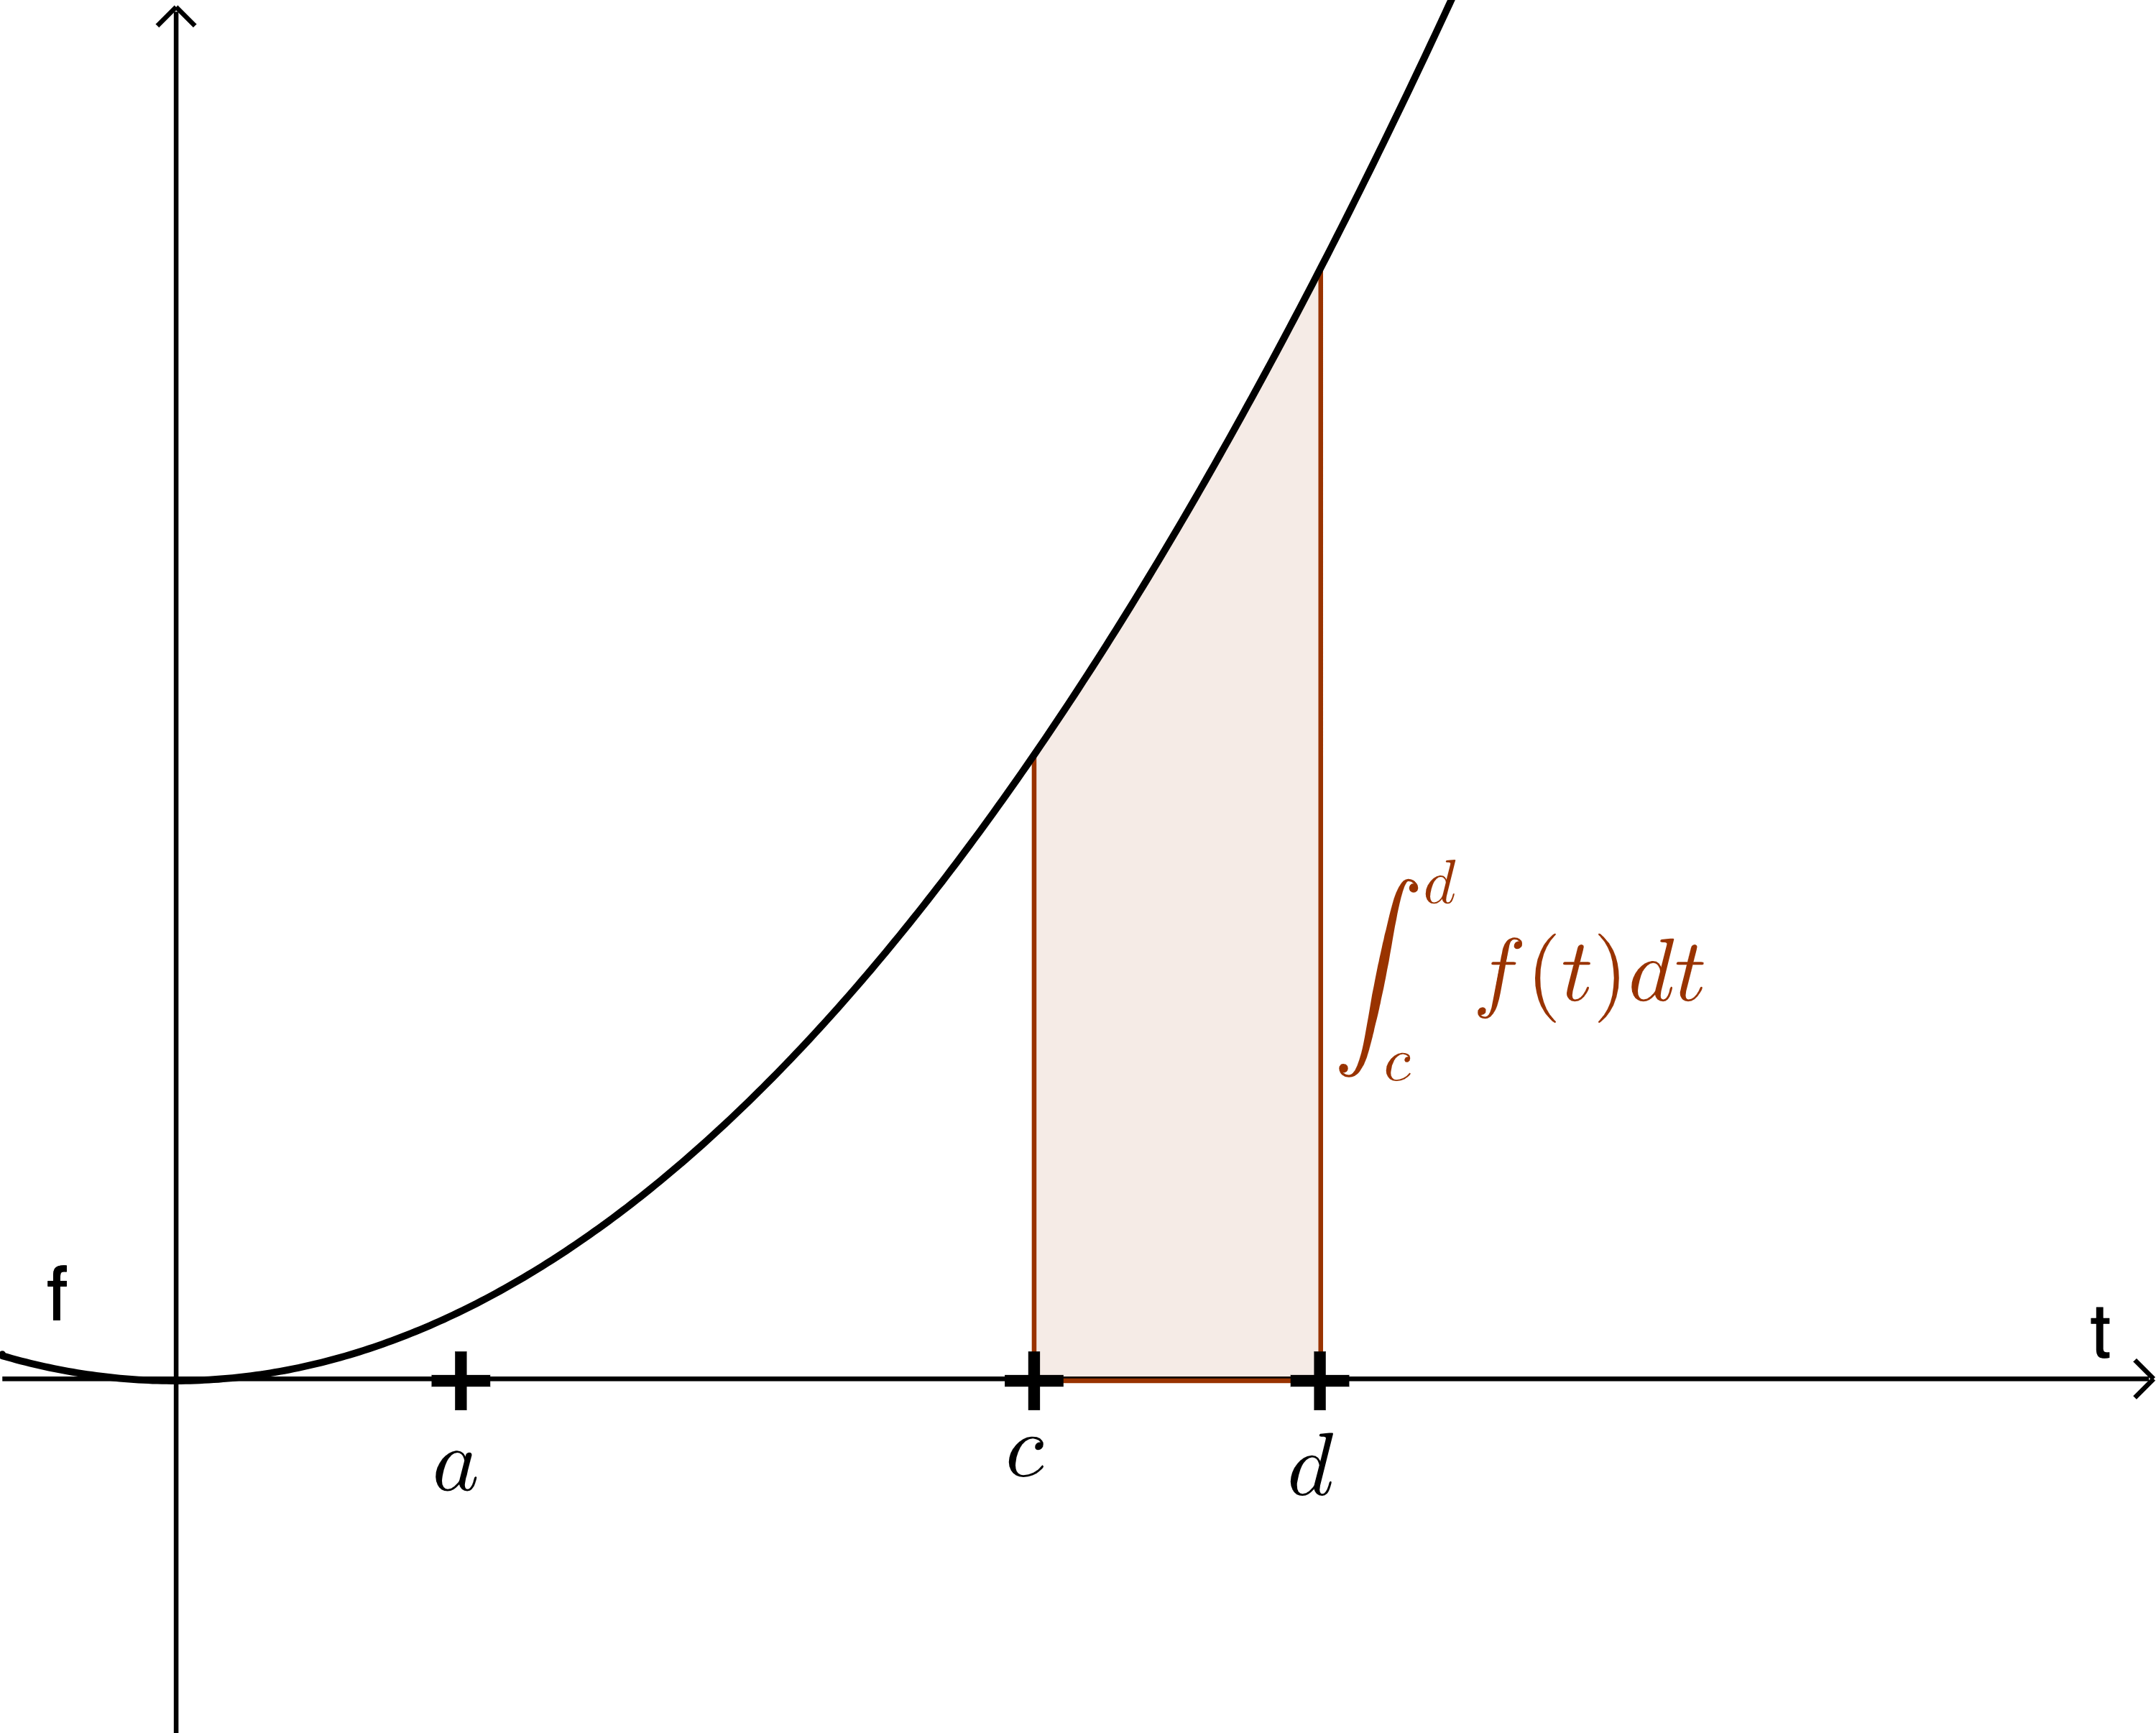
\includegraphics[width=\linewidth]{media/intcd.png}
	\endminipage\hfill
	\minipage{0.32\textwidth}
	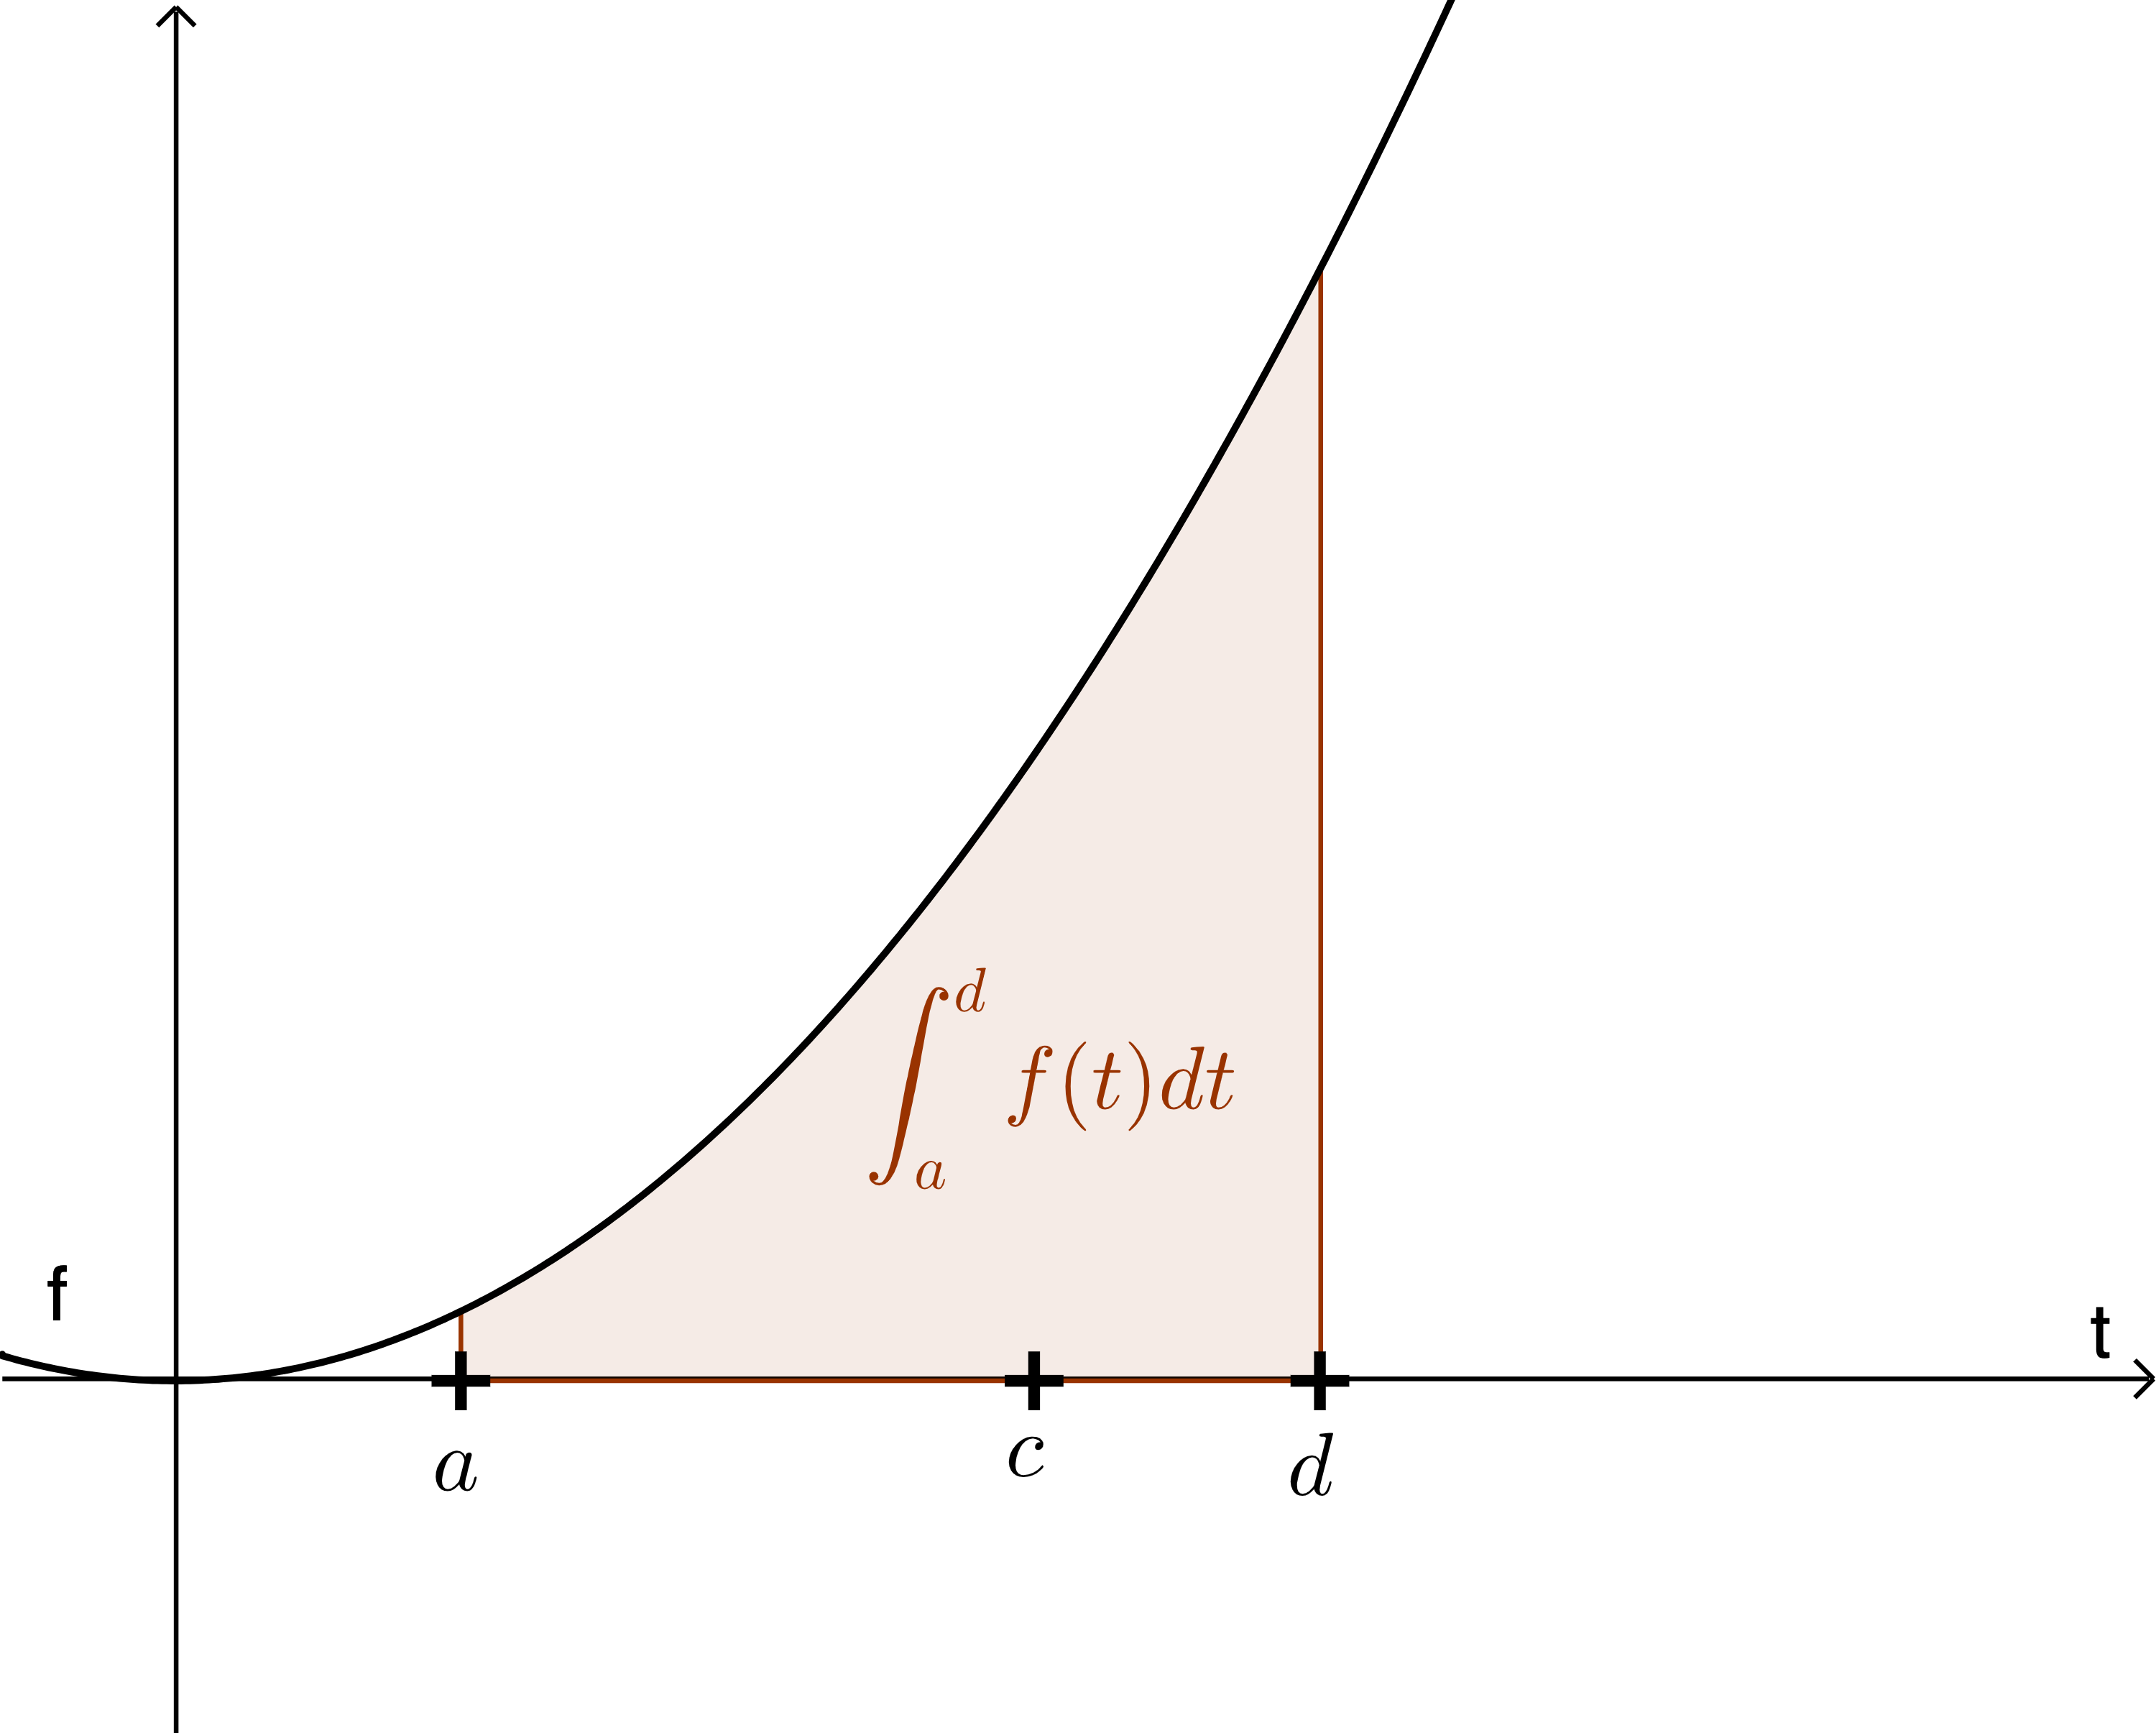
\includegraphics[width=\linewidth]{media/intd.png}
	\endminipage\hfill
	\minipage{0.32\textwidth}
	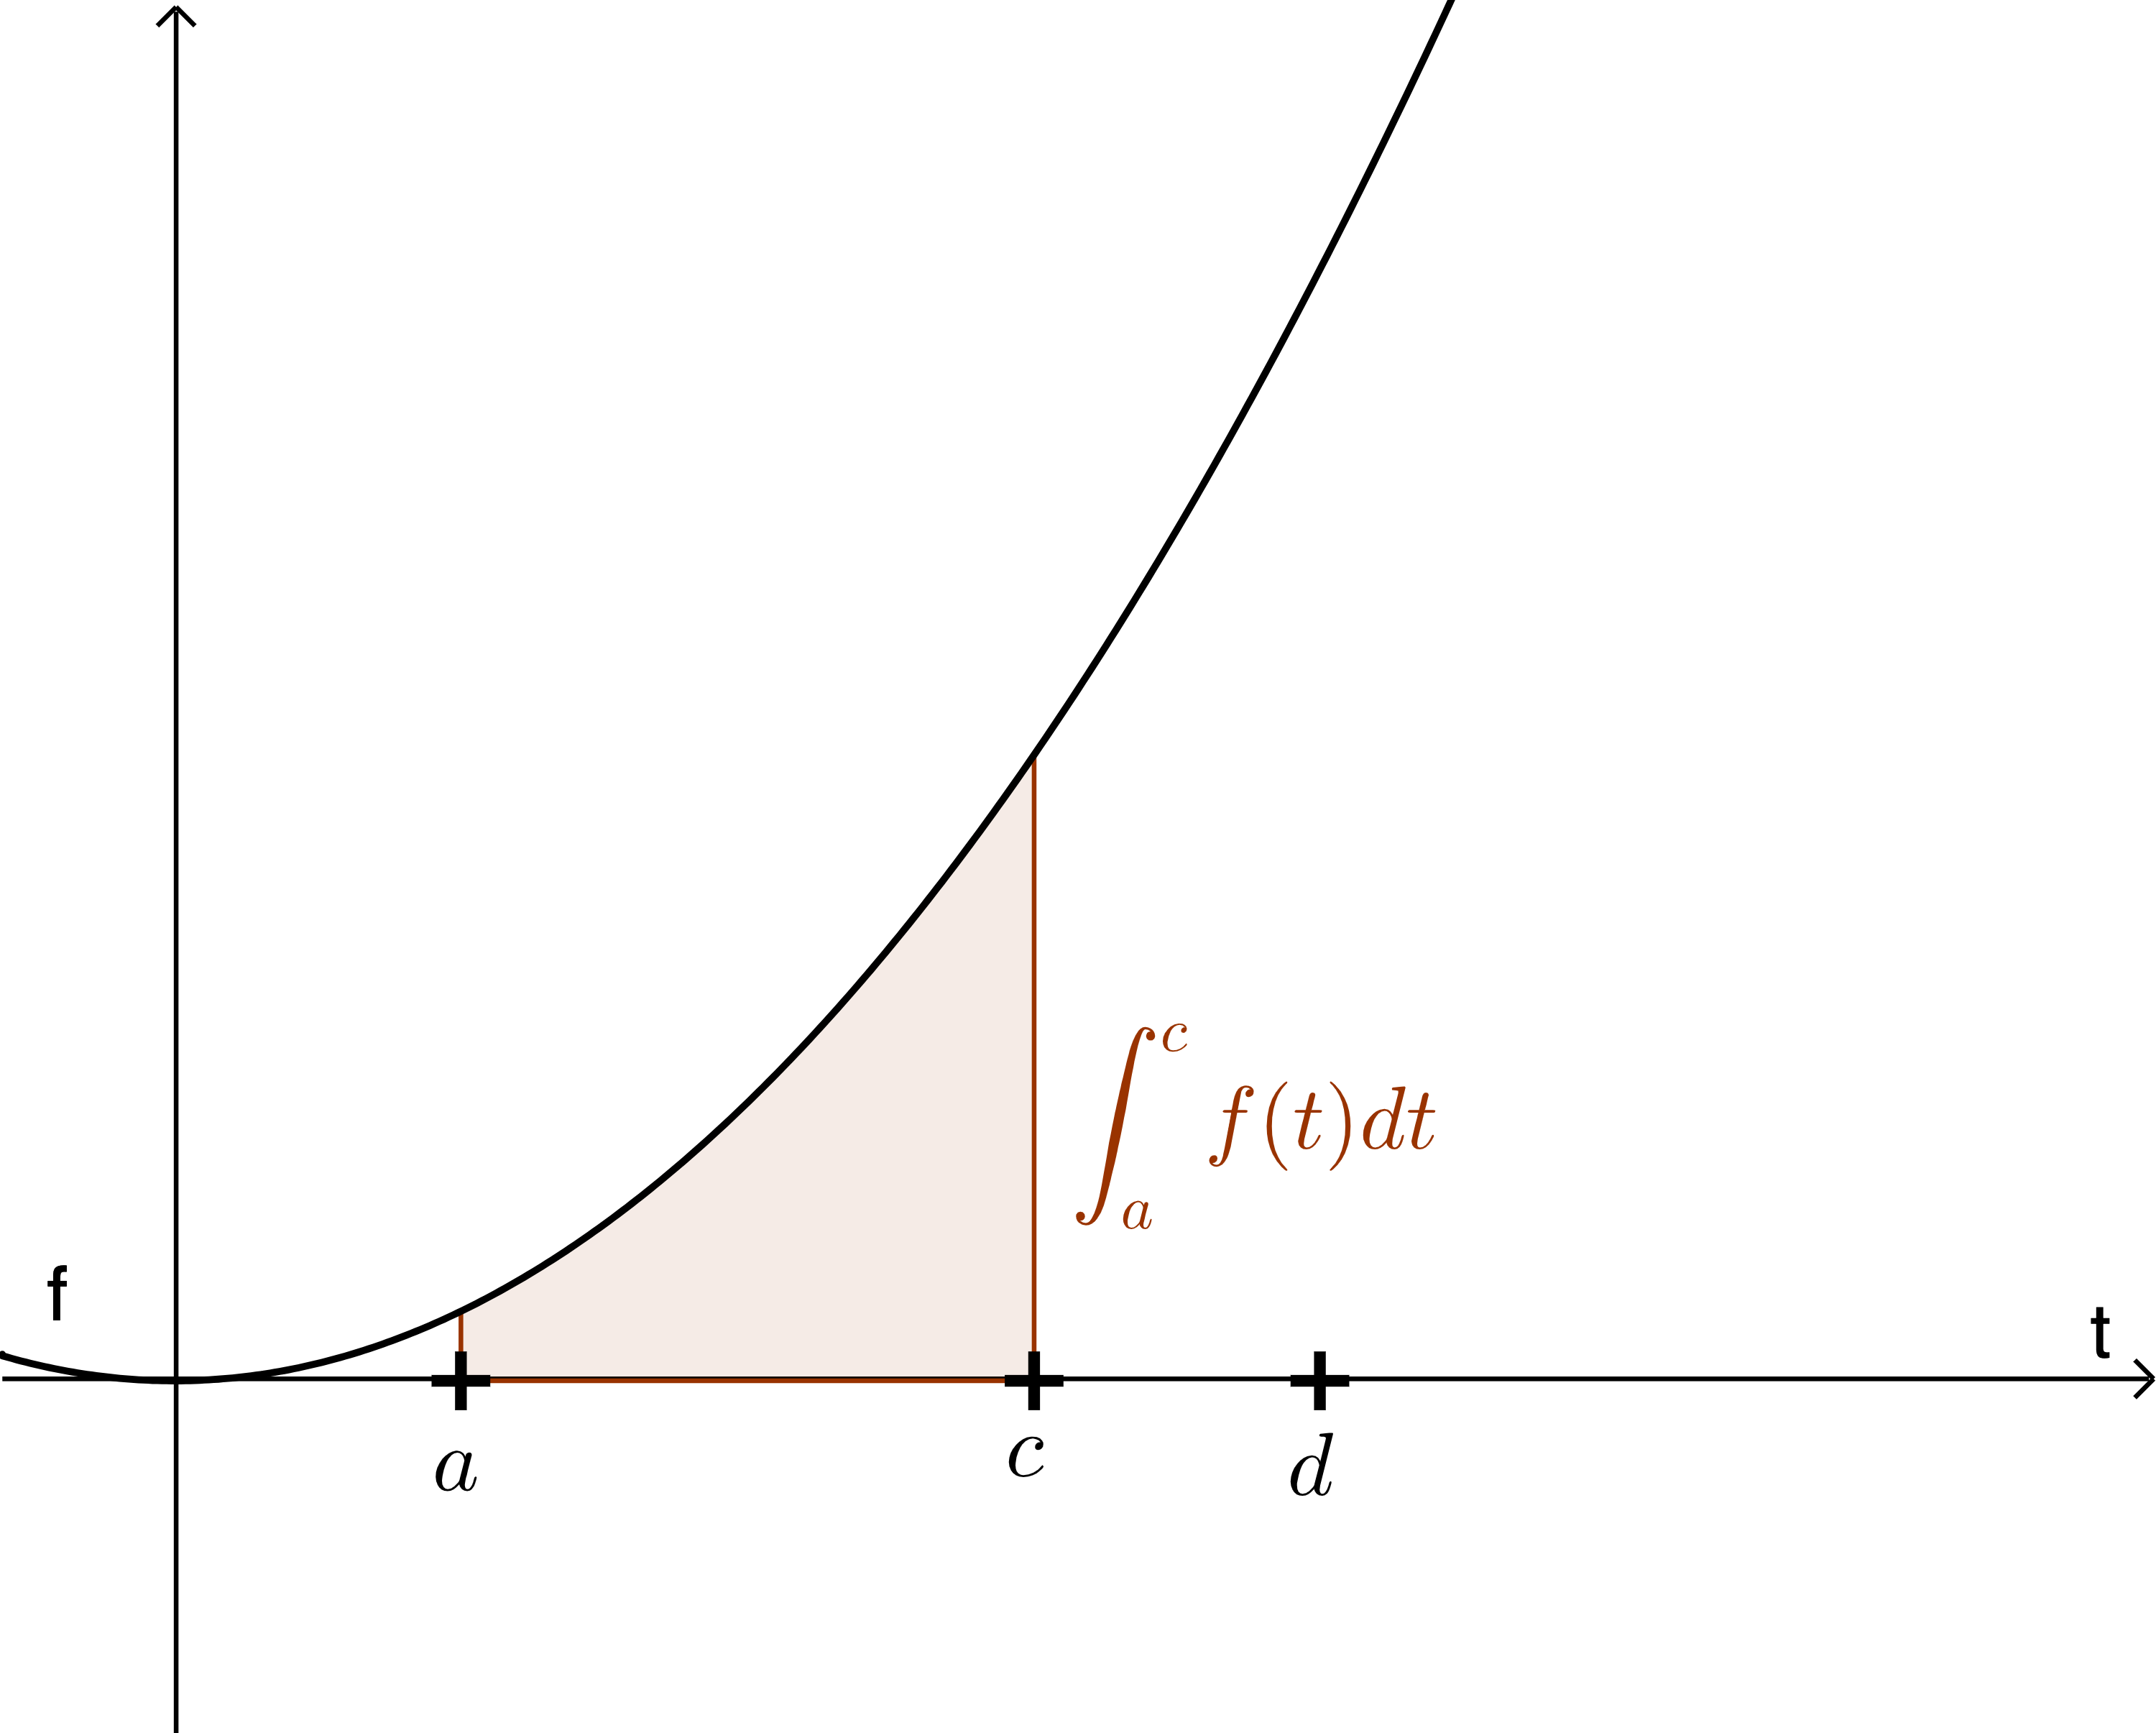
\includegraphics[width=\linewidth]{media/intac.png}
	\endminipage
\end{figure}





Es bleibt die Frage, ob es einen einfachen Weg gibt, eine Integralfunktion einer gegebenen Funktion $f$ zu bestimmen, ohne die Ober- und Untersumme zu berechnen.

\begin{satz}
	{Hauptsatz der Differential- und Integralrechnung}{Hauptsatz}
	Sei $f: \: [a,b] \rightarrow \R$ eine stetige Funktion. Sei $F_a(b)=\int_a^b f(x) \,dx$ eine Integralfunktion von $f$. Dann gilt:
	$$ \frac{d}{dx} F_a(x) = f(x) $$
	Kurz: Integralfunktionen sind Stammfunktionen von $f$.
\end{satz}
\textbf{Bemerkungen}
\begin{enumerate}
	\item Integralfunktionen von $f$ sind nach dem Hauptsatz Stammfunktionen von $f$.
	\item Zu einer gegebenen Funktion gibt es unendliche viele Stammfunktionen. Diese unterscheiden sich durch einen konstanten Summanden.
	\item Aus 1. und 2. folgt: Sei $F(x)$ eine beliebige Stammfunktion von $f$ und $F_0(x)$ die Integralfunktion von $f$ zur unteren Grenze $0$. Dann gibt es eine Konstante $c\in \R$ mit
	      $$F_0(x)=F(x)+c$$
	\item Folglich gilt für die bestimmten Integrale
	      $$ \int_{a}^{b} f(t) \, dt = F_0(b) - F_0(a) = \left(F(b)+c\right)-\left(F(a)+c\right) = F(b) -F(a) $$
\end{enumerate}

\begin{satz}
	{Berechnung von bestimmten Integralen}{}
	Sei $f: \: [a,b] \rightarrow \R$ eine stetige Funktion. Sei $F$ eine \textbf{beliebige} Stammfunktion von $f$. Dann gilt:
	$$ \int_{a}^{b} f(x) \, dx = F(b) -F(a) $$

	Notation: Für $F(b) -F(a)$ schreibt man häufig $\left[F(x)\right]_a^b$
\end{satz}
\begin{bsp}
	{Berechnung eines bestimmten Integrals}{}
	$$\int_1^2 \left(\frac{1}{4} x^2+x+2\right) \, dx=?$$

	Bestimme eine Stammfunktion (anti-Differenzieren): $F(x)=\frac{1}{12}x^3+\frac{1}{2}x^2+2x$.

	Dann folgt
	\begin{align*}
		\int_1^2 \left(\frac{1}{4} x^2+x+2\right) \, dx & =\left[\frac{1}{12}x^3+\frac{1}{2}x^2+2x\right]_1^2                                                          \\
		                                                & = \left(\frac{1}{12}2^3+\frac{1}{2}2^2+2\cdot 2\right) -\left(\frac{1}{12}1^3+\frac{1}{2}1^2+2\cdot 1\right) \\
		                                                & = \frac{49}{12}
	\end{align*}
	\begin{center}
		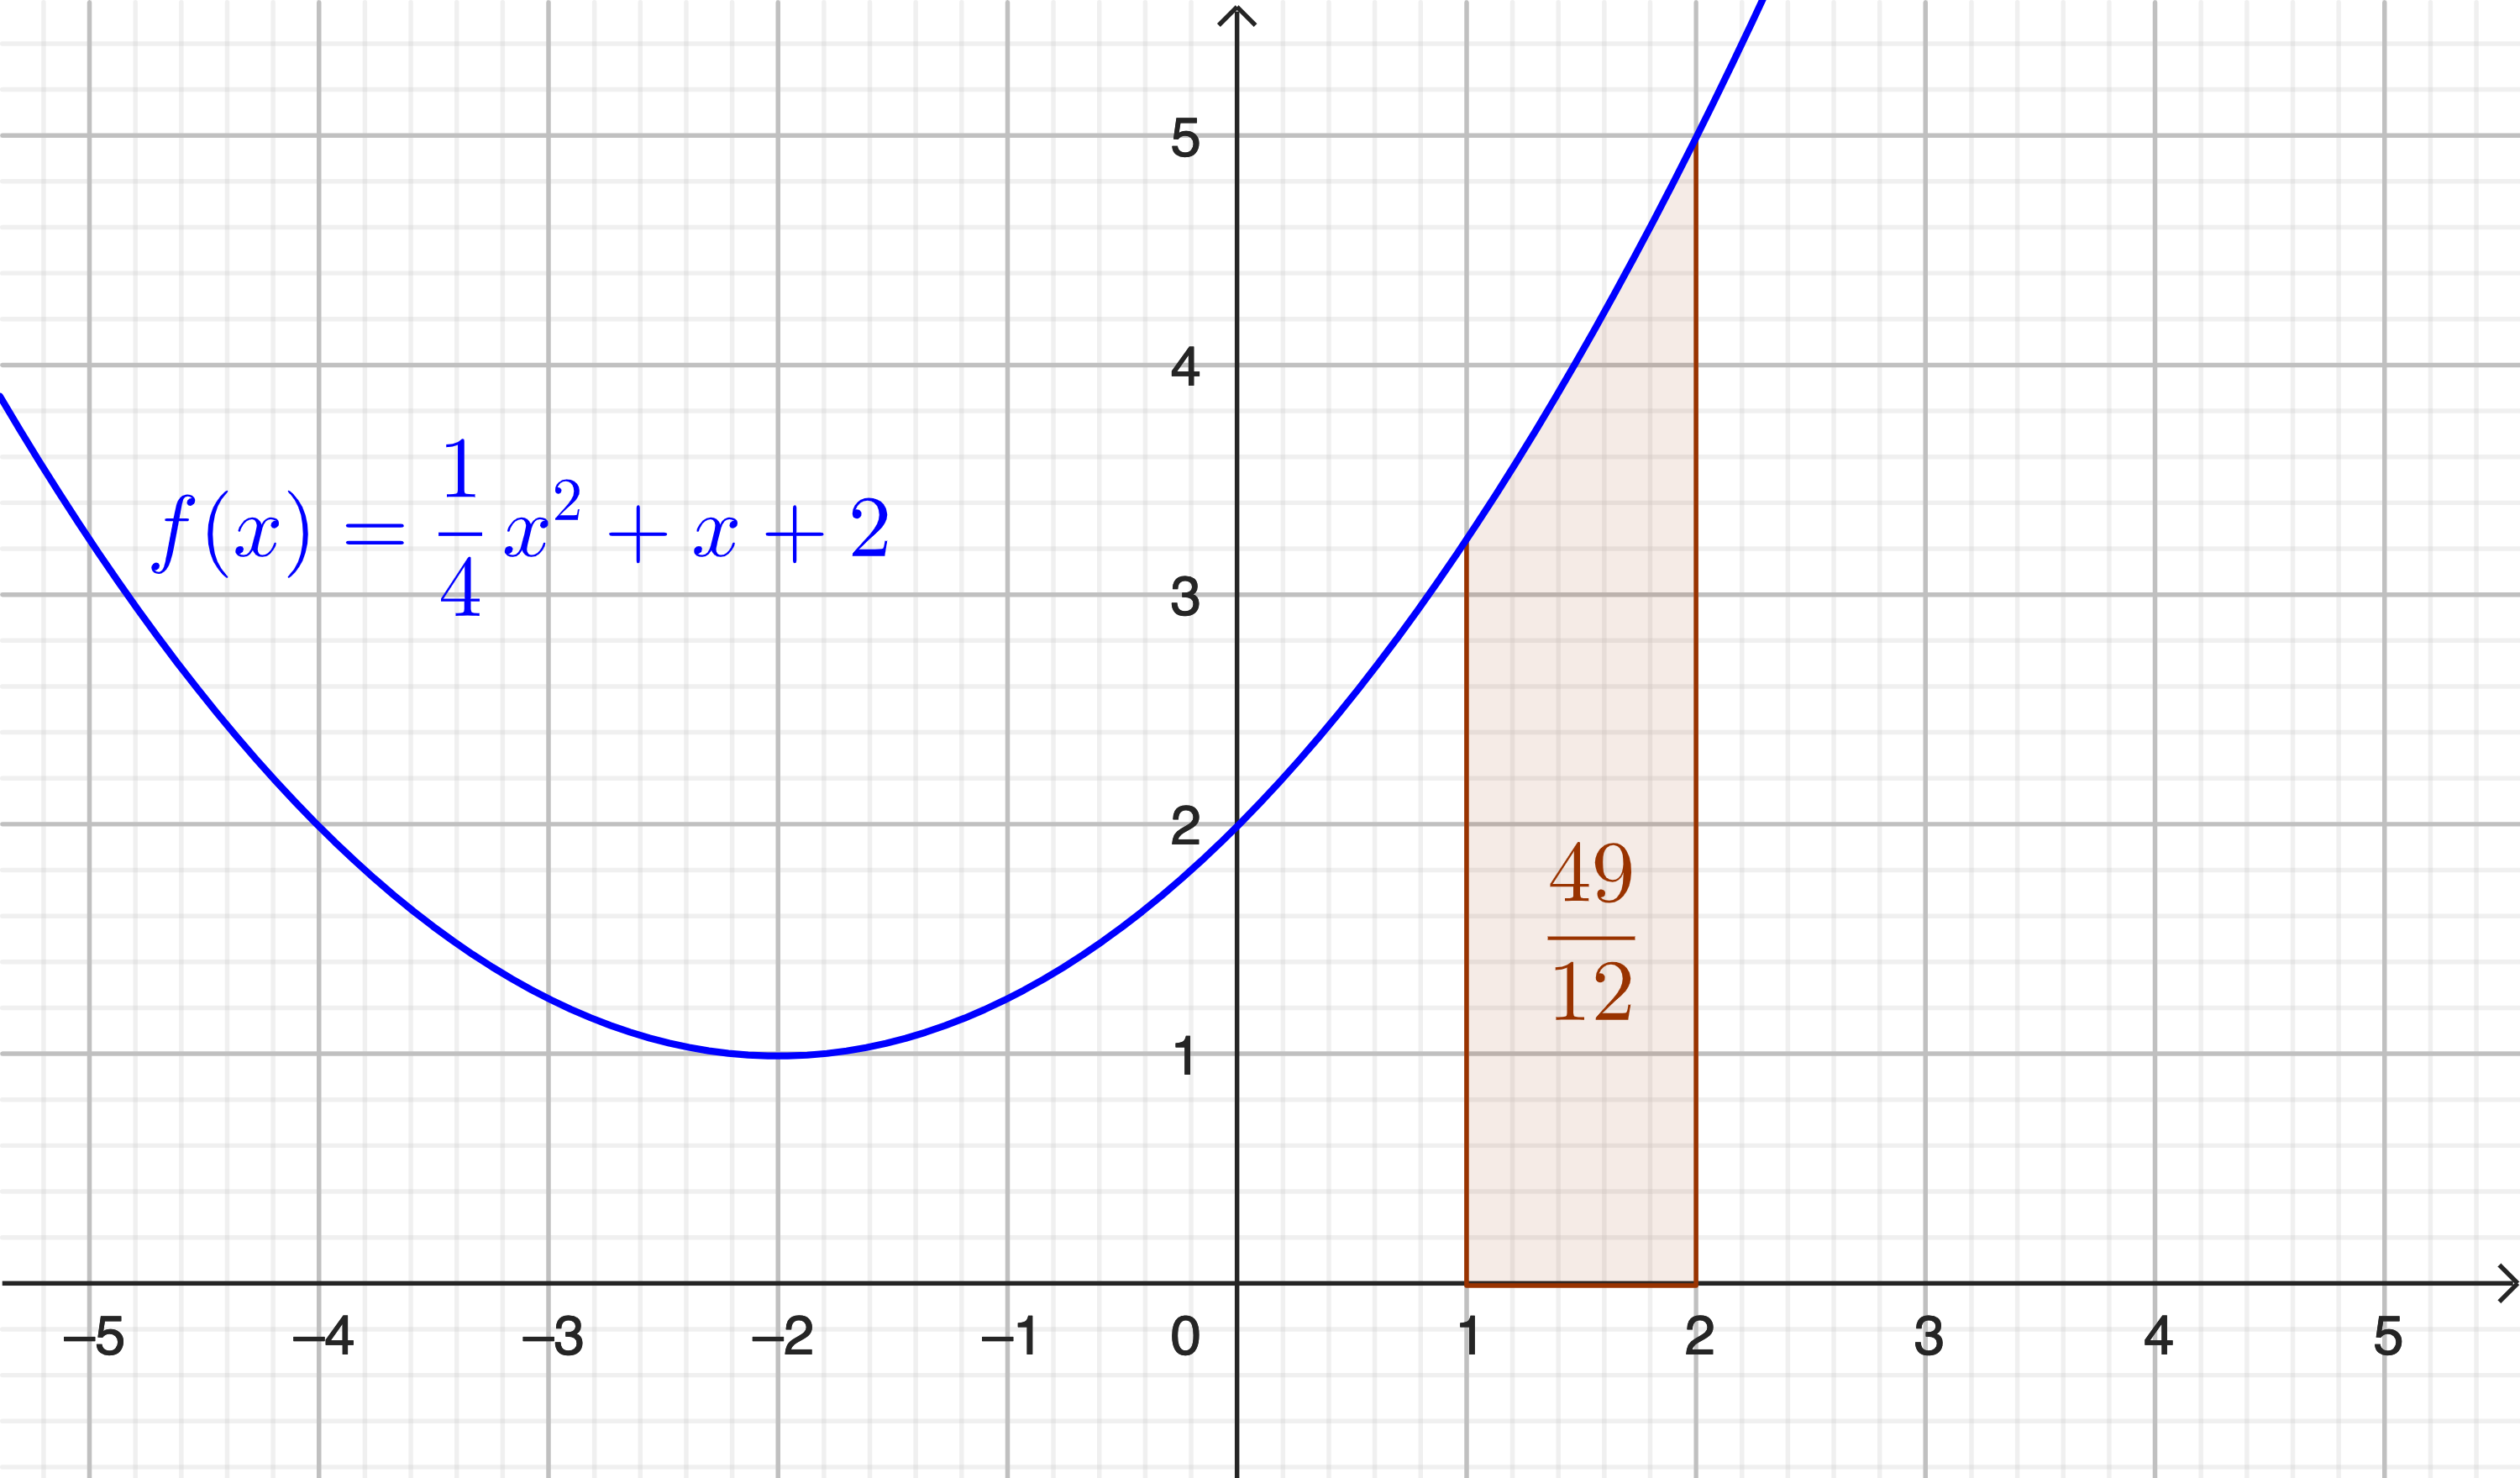
\includegraphics[width = 0.8 \textwidth]{media/bspHauptsatz.png}
	\end{center}
\end{bsp}
\begin{proof}[Beweis des Hauptsatzes der Differential- und Integralrechnung]
	Beim Bestimmen der Ableitung der Integralfunktion $F_a$ helfen uns keine Ableitungsregeln. Wir müssen auf die Definition der Ableitung zurückgreifen.
	Zur Erinnerung: Die Ableitung einer Funktion $f$ ist definiert durch den Differenzialquotienten:
	$$ \frac{d}{dx} f(x)=\lim_{h\rightarrow0} \frac{f(x+h)-f(x)}{h}$$
	Angewendet auf unsere Integralfunktion heisst das:
	$$ \frac{d}{dx} F_a(x)=\lim_{h\rightarrow0} \frac{F_a(x+h)-F_a(x)}{h}$$

	Für die folgenden Überlegungen gehen wir davon aus, dass $h>0$ ist. Der Fall $h<0$ geht analog.

	Schauen wir uns den Zähler $F_a(x+h)-F_a(x)$ etwas genauer an: Er entspricht dem Flächeninhalt der schraffierten Figur:
	\begin{center}
		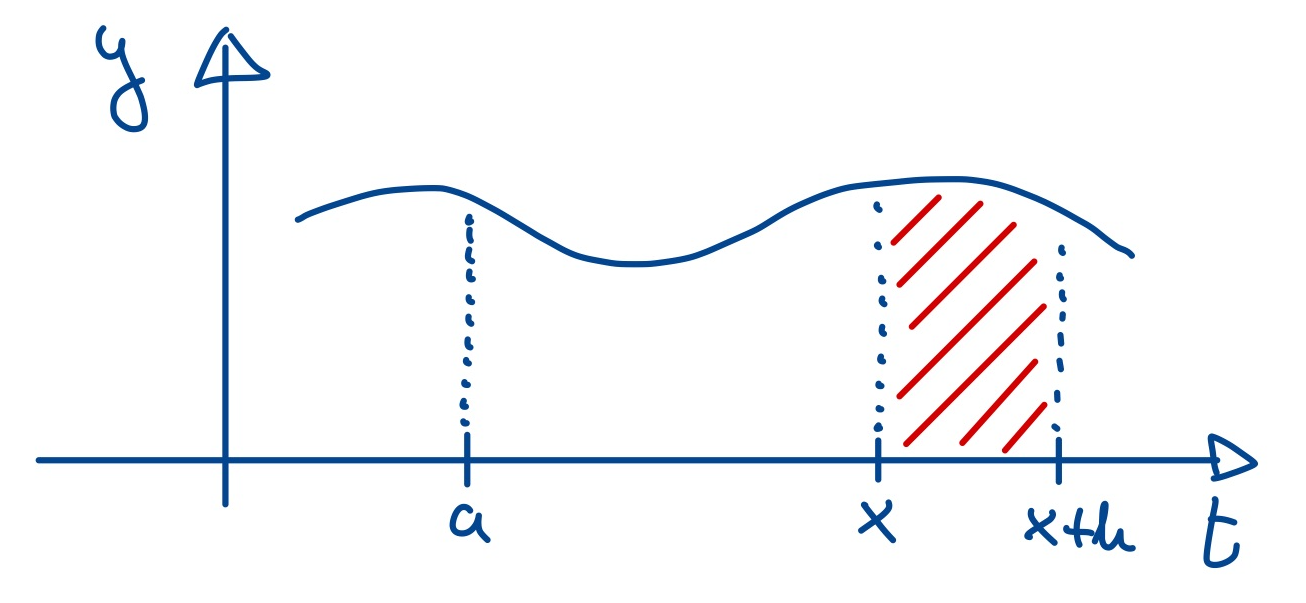
\includegraphics[width = 0.5 \textwidth]{media/BewHauptsatz1.png}
	\end{center}

	Dieser Flächeninhalt können wir nun von oben und von unten durch Rechtecke abschätzen:

	\begin{figure}[!htb]
		\minipage{0.4\textwidth}
		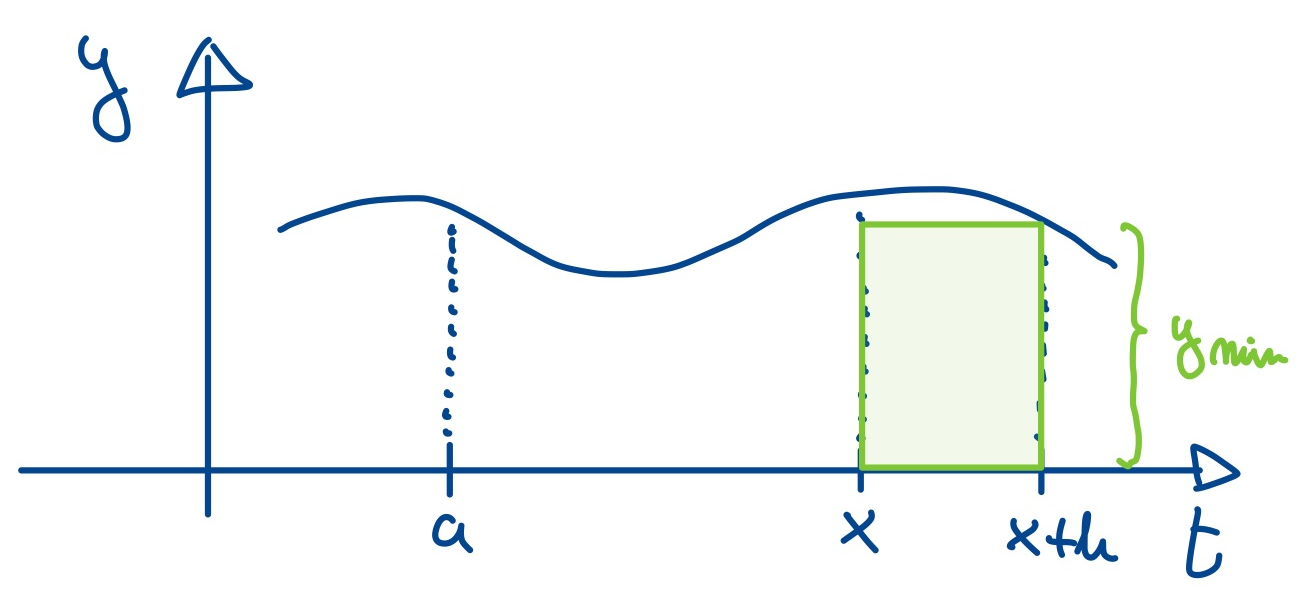
\includegraphics[width=\linewidth]{media/BewHauptsatz2.png}
		\endminipage\hfill
		\minipage{0.4\textwidth}
		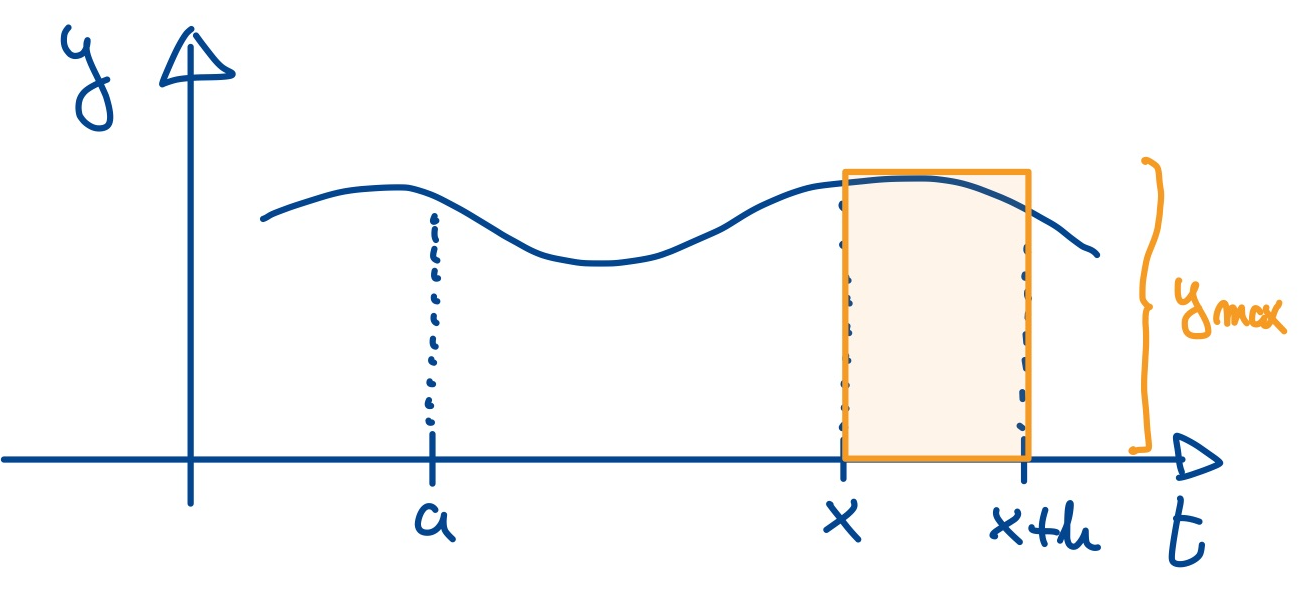
\includegraphics[width=\linewidth]{media/BewHauptsatz3.png}
		\endminipage
	\end{figure}

	Wobei $y_{\text{min}}$  und $y_{\text{max}}$  der kleinste, bzw. grösste Wert von $f(t)$ im Intervall $[x,x+h]$ sind.
	Daraus folgt die Ungleichung
	$$h\cdot y_{\text{min}}\le F_a (x+h)-F_a (x)\le h\cdot y_{\text{max}}$$
	Indem wir beide Seiten der Ungleichung durch $h$ teilen erhalten wir
	$$ y_{\text{min}}\le \frac{F_a (x+h)-F_a (x)}{h}\le y_{\text{max}}$$

	Lassen wir nun $h$ gegen Null streben. Wenn das Intervall $[x,x+h]$ immer kleiner wird, nähert sich der kleinste Wert $y_{\text{min}}$ immer mehr dem Funktionswert $f(x)$. Analog strebt $y_{\text{max}}$ nach $f(x)$. Der mittlere Term $\frac{F_a (x+h)-F_a (x)}{h}$ entspricht für $h \rightarrow0$ genau der Ableitung von $F_a$. Somit gilt:
	$$f(x)\le \frac{d}{dx} F_a (x)\le f(x)$$
	Daraus folgt
	$$\frac{d}{dx} F_a (x)= f(x)$$

\end{proof}

\clearpage
\begin{ueb}
	{}{}
	\begin{enumerate}
		\item Berechnen Sie mit dem Hauptsatz das bestimmte Integral und vergleichen Sie die Ergebnisse. Erklären Sie das Gefundene mithilfe von Skizzen/Geogebra.
		      \begin{enumerate}
			      \item \(\displaystyle \int_0^2 x^2 \, dx \) vergleichen mit:
			            \begin{enumerate}
				            \item \(\displaystyle \int_0^2 (x^2 + 1) \, dx \)
				            \item \(\displaystyle \int_0^2 (x + 1)^2 \, dx \)
				            \item \(\displaystyle \int_{-1}^1 (x + 1)^2 \, dx \)
			            \end{enumerate}
			      \item \(\displaystyle \int_0^4 \sqrt{x} \, dx \) vergleichen mit:
			            \begin{enumerate}
				            \item \(\displaystyle \int_0^4 \sqrt{x + 1} \, dx \)
				            \item \(\displaystyle \int_{-1}^3 \sqrt{x + 1} \, dx \)
				            \item \(\displaystyle \int_1^5 \sqrt{x - 1} \, dx \)
			            \end{enumerate}
		      \end{enumerate}
		\item \textbf{Polynomfunktionen}
		      \begin{enumerate}
			      \item \(\displaystyle \int_0^2 4x^3 \, dx \)
			      \item \(\displaystyle \int_2^4 \frac{1}{5}x^3 \, dx \)
			      \item \(\displaystyle \int_{-1}^2 (x^2 + 3) \, dx \)
			      \item \(\displaystyle \int_3^5 \left( \frac{1}{2}x - 2 \right) \, dx \)
			      \item \(\displaystyle \int_0^3 2x(1 - x) \, dx \)
			      \item \(\displaystyle \int_{-3}^3 (x - 1)^2 \, dx \)
		      \end{enumerate}

		\item \textbf{Gebrochenrationale Funktionen} (Tipp: $\left(\ln(x)\right)'= \frac{1}{x}$)
		      \begin{enumerate}
			      \item \(\displaystyle \int_2^4 \frac{1}{x^2} \, dx \)
			      \item \(\displaystyle \int_{-1}^{-0.5} \frac{3}{x^5} \, dx \)
			      \item \(\displaystyle \int_1^2 \left( 2x - \frac{2}{x} \right) \, dx \)
			      \item \(\displaystyle \int_1^3 \left( 4x - \frac{3}{x} + \frac{2}{x^2} \right) \, dx \)
			      \item \(\displaystyle \int_3^5 \frac{x - 2}{x} \, dx \)
			      \item \(\displaystyle \int_2^3 \frac{x^2 + 4x + 3}{x} \, dx \)
		      \end{enumerate}

		\item \textbf{Wurzelfunktionen}
		      \begin{enumerate}
			      \item \(\displaystyle \int_1^4 3\sqrt{x} \, dx \)
			      \item \(\displaystyle \int_1^4 \frac{1}{\sqrt{x}} \, dx \)
			      \item \(\displaystyle \int_0^8 \sqrt[3]{x} \, dx \)
			      \item \(\displaystyle \int_0^1 x\sqrt{x} \, dx \)
			      \item \(\displaystyle \int_1^4 (2x + 6\sqrt{x}) \, dx \)
			      \item \(\displaystyle \int_1^4 \sqrt{\frac{3}{x^3}} \, dx \)
		      \end{enumerate}

		\item \textbf{Winkelfunktionen}
		      \begin{enumerate}
			      \item \(\displaystyle \int_0^{\frac{\pi}{2}} \sin(t) \, dt \)
			      \item \(\displaystyle \int_\pi^{2\pi} \cos(t) \, dt \)
			      \item \(\displaystyle \int_0^{\frac{\pi}{3}} -2\sin(t) \, dt \)
			      \item \(\displaystyle \int_0^{\pi} (4\sin(t) - 3\cos(t)) \, dt \)
			            % \item \(\displaystyle \int_0^{\frac{7\pi}{4}} \frac{1}{\cos^2(t)} \, dt \)
			            % \item \(\displaystyle \int_{\frac{3\pi}{4}}^{\frac{5\pi}{4}} \tan(t) \, dt \)
		      \end{enumerate}

		\item \textbf{Exponentialfunktionen}
		      \begin{enumerate}
			      \item \(\displaystyle \int_{-1}^1 e^{x+1} \, dx \)
			      \item \(\displaystyle \int_{-1}^0 (2x - e^x) \, dx \)
			      \item \(\displaystyle \int_0^1 \pi \cdot e^x \, dx \)
			      \item \(\displaystyle \int_0^2 (e^x - x^e) \, dx \)
			      \item \(\displaystyle \int_1^2 \left(e^x + \frac{1}{x}\right) \, dx \)
			            % \item \(\displaystyle \int_0^1 10^x \, dx \)
		      \end{enumerate}

		\item \textbf{Einfache Substitutionsregel}
		      \begin{enumerate}
			      \item \(\displaystyle \int_2^5 (2x - 3)^4 \, dx \)
			      \item \(\displaystyle \int_0^6 (5 - 2x)^3 \, dx \)
			      \item \(\displaystyle \int_2^3 \frac{4}{(1 - x)^2} \, dx \)
			      \item \(\displaystyle \int_0^{\frac{\pi}{2}} \sin(3t) \, dt \)
			      \item \(\displaystyle \int_{-\frac{3}{4}}^{\frac{3}{4}} \cos(\pi t) \, dt \)
			      \item \(\displaystyle \int_0^\pi \left(\frac{1}{\pi} + \cos(-2t)\right) \, dt \)
			      \item \(\displaystyle \int_{1/2}^5 \frac{2}{3} e^{4x} \, dx \)
			      \item \(\displaystyle \int_0^6 e^{6 - x} \, dx \)
			      \item \(\displaystyle \int_{-\pi}^\pi (e^x - e^{-x}) \, dx \)
			      \item \(\displaystyle \int_{12}^{24} \frac{1}{\sqrt{2x + 1}} \, dx \)
			      \item \(\displaystyle \int_2^5 \frac{9}{3x - 5} \, dx \)
			            %\item \(\displaystyle \int_{-3}^0 \ln(2) \cdot 2^{-\frac{1}{3}x} \, dx \)
		      \end{enumerate}


	\end{enumerate}

\end{ueb}


\clearpage
\emph{Lösungen}

\begin{enumerate}
	\item Vergleichen der Resultate
	      \begin{enumerate}
		      \item
		            \[
			            \int_0^2 x^2 \, dx
			            = \left[\frac{1}{3}x^3\right]_0^2
			            = \frac{8}{3}
		            \]
		            \begin{enumerate}
			            \item
			                  \[
				                  \int_0^2 (x^2+1)\,dx
				                  = \left[\frac{1}{3}x^3+x\right]_0^2
				                  = 8/3 + 2
				                  = \frac{14}{3}
			                  \]
			            \item
			                  \[
				                  \int_0^2 (x+1)^2\,dx
				                  = \left[\frac{1}{3}x^3+x^2+x\right]_0^2
				                  = \frac{26}{3}
			                  \]
			            \item
			                  \[
				                  \int_{-1}^1 (x+1)^2\,dx
				                  = \left[\frac{1}{3}x^3+x^2+x\right]_{-1}^1
				                  = \frac{8}{3}
			                  \]
		            \end{enumerate}

		      \item
		            \[
			            \int_0^4 \sqrt{x}\,dx
			            = \left[\frac{2}{3}x^{3/2}\right]_0^4
			            = \frac{16}{3}
		            \]
		            \begin{enumerate}
			            \item
			                  \[
				                  \int_0^4 \sqrt{x+1}\,dx
				                  = \left[\frac{2}{3}(x+1)^{3/2}\right]_0^4
				                  = \frac{10\sqrt{5}}{3}-\frac{2}{3}
			                  \]
			            \item
			                  \[
				                  \int_{-1}^3 \sqrt{x+1}\,dx
				                  = \left[\frac{2}{3}(x+1)^{3/2}\right]_{-1}^3
				                  = \frac{16}{3}
			                  \]
			            \item
			                  \[
				                  \int_1^5 \sqrt{x-1}\,dx
				                  = \left[\frac{2}{3}(x-1)^{3/2}\right]_1^5
				                  = \frac{16}{3}
			                  \]
		            \end{enumerate}
	      \end{enumerate}

	\item Polynomfunktionen
	      \begin{enumerate}
		      \item
		            \[
			            \int_0^2 4x^3\,dx
			            = \left[x^4\right]_0^2
			            = 16
		            \]
		      \item
		            \[
			            \int_2^4 \frac{1}{5}x^3\,dx
			            = \left[\frac{1}{20}x^4\right]_2^4
			            = 12
		            \]
		      \item
		            \[
			            \int_{-1}^2 (x^2+3)\,dx
			            = \left[\frac{1}{3}x^3+3x\right]_{-1}^2
			            = 12
		            \]
		      \item
		            \[
			            \int_3^5 \left(\frac{1}{2}x-2\right)\,dx
			            = \left[\frac{1}{4}x^2-2x\right]_3^5
			            = 0
		            \]
		      \item
		            \[
			            \int_0^3 2x(1-x)\,dx
			            = \left[x^2-\frac{2}{3}x^3\right]_0^3
			            = -9
		            \]
		      \item
		            \[
			            \int_{-3}^3 (x-1)^2\,dx
			            = \int_{-3}^3 (x^2-2x+1) \,dx
			            = \left[\frac{1}{3}x^3-x^2+x\right]_{-3}^3
			            = 24
		            \]
	      \end{enumerate}

	\item Gebrochenrationale Funktionen
	      \begin{enumerate}
		      \item
		            \[
			            \int_2^4 \frac{1}{x^2}\,dx
			            =  \int_2^4 x^{-2}\,dx
			            = \left[-x^{-1}\right]_2^4
			            = \frac{1}{4}
		            \]
		      \item
		            \[
			            \int_{-1}^{-0.5} \frac{3}{x^5}\,dx
			            = \left[-\frac{3}{4}x^{-4}\right]_{-1}^{-0.5}
			            = -11.25
		            \]
		      \item
		            \[
			            \int_1^2 \left(2x-\frac{2}{x}\right)\,dx
			            = \left[x^2-2\ln(x)\right]_1^2
			            = 3-2\ln(2)\approx 1.61
		            \]
		      \item
		            \[
			            \int_1^3 \left(4x-\frac{3}{x}+\frac{2}{x^2}\right)\,dx
			            = \left[2x^2-3\ln(x)-\frac{2}{x}\right]_1^3
			            = \frac{52}{3}-3\ln(3)\approx 14.04
		            \]
		      \item
		            \[
			            \int_3^5 \frac{x-2}{x}\,dx
			            = \int_3^5 \left(1-2\cdot\frac{1}{x}\right)\,dx
			            = \left[x-2\ln(x)\right]_3^5
			            = 2\ln\!\left(\frac{3}{5}\right)+2 \approx 0.98
		            \]
		      \item
		            \[
			            \int_2^3 \frac{x^2+4x+3}{x}\,dx
			            = \left[\frac{1}{2}x^2+4x+3\ln(x)\right]_2^3
			            = 3\ln\!\left(\frac{3}{2}\right)+\frac{13}{2}\approx 7.72
		            \]
	      \end{enumerate}

	\item Wurzelfunktionen
	      \begin{enumerate}
		      \item
		            \[
			            \int_1^4 3\sqrt{x}\,dx
			            =  \int_1^4 3 x^{1/2}\,dx
			            = \left[2x^{3/2}\right]_1^4
			            = 14
		            \]
		      \item
		            \[
			            \int_1^4 \frac{1}{\sqrt{x}}\,dx
			            = \int_1^4 x^{-1/2}\,dx
			            = \left[2\sqrt{x}\right]_1^4
			            = 2
		            \]
		      \item
		            \[
			            \int_0^8 \sqrt[3]{x}\,dx
			            = \int_0^8 x^{1/3}\,dx
			            = \left[\frac{3}{4}x^{4/3}\right]_0^8
			            = 12
		            \]
		      \item
		            \[
			            \int_0^1 x\sqrt{x}\,dx
			            = \int_0^1 x^{3/2}\,dx
			            = \left[\frac{2}{5}x^{5/2}\right]_0^1
			            = \frac{2}{5}
		            \]
		      \item
		            \[
			            \int_1^4 (2x+6\sqrt{x})\,dx
			            = \left[x^2+4x^{3/2}\right]_1^4
			            = 43
		            \]
		      \item
		            \[
			            \int_1^4 \sqrt{\frac{3}{x^3}}\,dx
			            = \int_1^4 \sqrt{3}\cdot x^{-3/2}\,dx
			            = \left[\sqrt{3}\cdot (-2)\cdot x^{-1/2}\right]_1^4
			            = \sqrt{3}
		            \]
	      \end{enumerate}

	\item Winkelfunktionen
	      \begin{enumerate}
		      \item
		            \[
			            \int_0^{\frac{\pi}{2}} \sin(t)\,dt
			            = \left[-\cos(t)\right]_0^{\frac{\pi}{2}}
			            = 1
		            \]
		      \item
		            \[
			            \int_\pi^{2\pi} \cos(t)\,dt
			            = \left[\sin(t)\right]_\pi^{2\pi}
			            = 0
		            \]
		      \item
		            \[
			            \int_0^{\frac{\pi}{3}} -2\sin(t)\,dt
			            = \left[2\cos(t)\right]_0^{\frac{\pi}{3}}
			            = -1
		            \]
		      \item
		            \[
			            \int_0^{\pi} (4\sin(t)-3\cos(t))\,dt
			            = \left[-4\cos(t)-3\sin(t)\right]_0^{\pi}
			            = 8
		            \]
	      \end{enumerate}

	\item Exponentialfunktionen
	      \begin{enumerate}
		      \item
		            \[
			            \int_{-1}^ 1 e\cdot e^{x}\,dx
			            = \left[ e \cdot e^{x}\right]_{-1}^1
			            = e^2-1
		            \]
		      \item
		            \[
			            \int_{-1}^0 (2x-e^x)\,dx
			            = \left[x^2-e^x\right]_{-1}^0
			            = \frac{1}{e}-2
		            \]
		      \item
		            \[
			            \int_0^1 \pi\cdot e^x\,dx
			            = \left[\pi e^x\right]_0^1
			            = \pi(e-1)
		            \]
		      \item
		            \[
			            \int_0^2 (e^x-x^e)\,dx
			            = \left[e^x-\frac{1}{e+1}x^{e+1}\right]_0^2
			            \approx 2.85
		            \]
		      \item
		            \[
			            \int_1^2 \left(e^x+\frac{1}{x}\right)\,dx
			            = \left[e^x+\ln(x)\right]_1^2
			            \approx 5.36
		            \]
	      \end{enumerate}

	\item Einfache Substitutionsregel
	      \begin{enumerate}
		      \item
		            \[
			            \int_2^5 (2x-3)^4\,dx
			            = \left[\frac{1}{10}(2x-3)^5\right]_2^5
			            = 1680.6
		            \]
		      \item
		            \[
			            \int_0^6 (5-2x)^3\,dx
			            = \left[-\frac{1}{8}(5-2x)^4\right]_0^6
			            = -222
		            \]
		      \item
		            \[
			            \int_2^3 \frac{4}{(1-x)^2}\,dx
			            = \left[\frac{4}{1-x}\right]_2^3
			            = 2
		            \]
		      \item
		            \[
			            \int_0^{\frac{\pi}{2}} \sin(3t)\,dt
			            = \left[-\frac{1}{3}\cos(3t)\right]_0^{\frac{\pi}{2}}
			            = \frac{1}{3}
		            \]
		      \item
		            \[
			            \int_{-\frac{3}{4}}^{\frac{3}{4}} \cos(\pi t)\,dt
			            = \left[\frac{1}{\pi}\sin(\pi t)\right]_{-\frac{3}{4}}^{\frac{3}{4}}
			            = \frac{\sqrt{2}}{\pi}
		            \]
		      \item
		            \[
			            \int_0^\pi \left(\frac{1}{\pi}+\cos(-2t)\right)\,dt
			            = \left[\frac{t}{\pi}-\frac{1}{2}\sin(-2t)\right]_0^\pi
			            = 1
		            \]
		      \item
		            \[
			            \int_{1/2}^5 \frac{2}{3}e^{4x}\,dx
			            = \left[\frac{1}{6}e^{4x}\right]_{1/2}^5
			            = \frac{1}{6}\left(e^{20}-e^2\right)
		            \]
		      \item
		            \[
			            \int_0^6 e^{6-x}\,dx
			            = \left[-e^{6-x}\right]_0^6
			            = e^6-1
		            \]
		      \item
		            \[
			            \int_{-\pi}^{\pi} (e^x-e^{-x})\,dx
			            = \left[e^x+e^{-x}\right]_{-\pi}^{\pi}
			            = 0
		            \]
		      \item
		            \[
			            \int_{12}^{24} \frac{1}{\sqrt{2x+1}}\,dx
			            = \left[\sqrt{2x+1}\right]_{12}^{24}
			            = 2
		            \]
		      \item
		            \[
			            \int_2^5 \frac{9}{3x-5}\,dx
			            = \left[3\ln|3x-5|\right]_2^5
			            = 3\ln(10)
		            \]
	      \end{enumerate}
\end{enumerate}

% \begin{enumerate}
% 	\item Vergleichen der Resultate
% 	      \begin{enumerate}
% 		      \item $8/3$
% 		            \begin{enumerate}
% 			            \item $14/3 = 8/3 + 2$
% 			            \item $26/3$
% 			            \item $8/3$
% 		            \end{enumerate}
% 		      \item $16/3$
% 		            \begin{enumerate}
% 			            \item $\frac{10\sqrt{5}}{3} - \frac{2}{3}$
% 			            \item $16/3$
% 			            \item $16/3$
% 		            \end{enumerate}
% 	      \end{enumerate}

% 	\item Polynomfunktionen
% 	      \begin{enumerate}
% 		      \item 16
% 		      \item 12
% 		      \item 12
% 		      \item 0
% 		      \item -9
% 		      \item 24
% 	      \end{enumerate}

% 	\item Gebrochenrationale Funktionen
% 	      \begin{enumerate}
% 		      \item 1/4
% 		      \item $-11.25$
% 		      \item $3-\ln(2)\approx 1.61$
% 		      \item $\frac{52}{3} - 3\ln(3) \approx 14.04$
% 		      \item $2\ln(3/5) + 2 \approx 0.98$
% 		      \item $3\ln(3/2)+13/2 \approx 7.72$
% 	      \end{enumerate}

% 	\item Wurzelfunktionen
% 	      \begin{enumerate}
% 		      \item 14
% 		      \item 2
% 		      \item 12
% 		      \item 2/5
% 		      \item 43
% 		      \item $\sqrt{3}$
% 	      \end{enumerate}


% 	\item Winkelfunktionen
% 	      \begin{enumerate}
% 		      \item 1
% 		      \item 0
% 		      \item -1
% 		      \item 8
% 		            % \item 1
% 		            % \item $\frac{1}{2} \ln(2)$
% 	      \end{enumerate}

% 	\item Exponentialfunktionen
% 	      \begin{enumerate}
% 		      \item $e^2 -1$
% 		      \item $\frac{1}{e} -2$
% 		      \item $\pi (e-1)$
% 		      \item $\approx 2.85$
% 		      \item $\approx 5.36$
% 		            %\item $\approx 3.91$ 
% 	      \end{enumerate}

% 	\item Einfache Substitutionsregel
% 	      \begin{enumerate}
% 		      \item 1680.6
% 		      \item 0
% 		      \item 2
% 		      \item 1/3
% 		      \item $\sqrt{2} / \pi$
% 		      \item 1
% 		      \item $\frac{1}{6} \left(e^{20}-1\right)$
% 		      \item $e^{12}-1$
% 		      \item 0
% 		      \item 2
% 		      \item $3\ln(10)$
% 		            %\item 3 
% 	      \end{enumerate}
% \end{enumerate}


\clearpage
\subsection{Flächen und Volumen}

\subsubsection{Flächeninhalt zwischen Kurve und \(x\)-Achse}

Bei der Berechnung von Flächeninhalten muss man vorsichtig sein und sich klarmachen, welche Teile der Fläche beim Integral positiv und welche negativ gezählt werden.

\begin{bsp}
	{Musterbeispiel zur Flächenberechnung}{}
	Bestimmen Sie den Inhalt der endlichen Fläche, die von der Kurve \(y=x^3-x^2-6x\) und der \(x\)-Achse eingeschlossen wird.
	\vspace{16cm}

\end{bsp}

\clearpage
\begin{ueb}{Flächen unter Graphen von Polynomfunktionen}{}
	\begin{enumerate}
		\item Bestimmen Sie den Inhalt der endlichen Fläche, die von der gegebenen Kurve und der \(x\)-Achse eingeschlossen wird.
		      \begin{enumerate}
			      \item \(y=x^2-5x+4\)
			      \item \(y=x^3-2x^2-3x\)
			      \item \(y=x^4-10x^2+9\)
		      \end{enumerate}
		\item Der Graph der Funktion \(f(x) = ax-x^3\) schliesst im 1. Quadranten mit der \(x\)-Achse eine Fläche mit dem Inhalt \(A=9\) ein. Berechnen Sie \(a\).
		\item Der Graph einer Funktion 3. Grades hat in \(P=(1, 0)\) die Steigung \(m=1\) und berührt die \(x\)-Achse im Ursprung. Bestimmen Sie den Inhalt der endlichen Fläche zwischen dem Graphen und der \(x\)-Achse.
		\item Der Graph einer Funktion 3. Grades berührt die \(x\)-Achse im Ursprung, hat ein Extremum bei \(x=2\) und schliesst im 1. Quadranten mit der \(x\)-Achse eine Fläche mit dem Inhalt \(A=27\) ein. Bestimmen Sie die Funktionsgleichung und die Koordinaten des Wendepunktes.
	\end{enumerate}
\end{ueb}
\begin{ueb}{Flächen unter Graphen von allgemeinen Funktionen}{}
	\begin{enumerate}\setcounter{enumi}{4}
		\item Berechnen Sie den Inhalt der endlichen Fläche, die von der Kurve \(y=\sqrt{x}-\frac{1}{2}x\) und der \(x\)-Achse berandet wird.
		\item Welchen Inhalt hat die Fläche, die begrenzt wird von der \(x\)-Achse, der Kurve \(y=\sqrt{x}\) und der Normalen im Kurvenpunkt \(P=(4, y_p)\)?
		\item Bestimmen Sie den Inhalt eines der (unendlich vielen) Flächenstücke, die zwischen dem Graphen der Funktion und der \(x\)-Achse liegen:
		      \begin{enumerate}
			      \item \(f(x) = \sin(x)\)
			      \item \(f(x) = \sin(x) - \cos(x)\)
		      \end{enumerate}
		\item Bestimmen Sie den Wert der Parameters \(a>0\), sodass die Funktion \(f(x) = (a-x)\cdot \sqrt{x}\) mit der \(x\) Achse eine Fläche mit dem Inhalt \(A=64.8\) einschliesst.
		\item Bestimmen Sie den Inhalt der endlichen Fläche, die von der Kurve \(y=\frac{x^2-5x+4}{x}\) und der \(x\)-Achse eingeschlossen wird.
	\end{enumerate}
\end{ueb}

\clearpage
\emph{Lösungen:}
\begin{enumerate}
	\item Flächenberechnung
	      \begin{enumerate}
		      \item \(A=\frac{9}{2}\)
		      \item \(A= \frac{71}{6}\)
		      \item \(A=52.26\bar{6}\)
	      \end{enumerate}
	\item \(a=6\)
	\item \(f(x)=x^3 - x^2\); \(A=\frac{1}{12}\)
	\item \(f(x)= -4x^3+12x^2\),  Wendepunkt: \(W=(1, 8)\)
	\item \(A=\frac{4}{3}\)
	\item \(A=\frac{35}{6}\)
	\item Flächenberechnung mit trigonometrischen Funktionen:
	      \begin{enumerate}
		      \item \(A=2\)
		      \item \(A=2\sqrt{2}\)
	      \end{enumerate}
	\item \(a=9\)
	\item \(A=1.95\)
\end{enumerate}













































\clearpage
\subsubsection{Die Fläche zwischen zwei Graphen}

Im Folgenden werden Sie lernen, wie man Flächeninhalte von Gebieten berechnen kann, die von zwei Funktionsgraphen begrenzt sind. Dabei gilt die folgende Grundidee:
\begin{satz}
	{Der Satz des toten Wals}{}
	Das Volumen eines Walfs ändert sich nicht, wenn er stirbt.
\end{satz}
Was damit gemeint ist, sehen wir im folgenden Beispiel.
\begin{bsp}
	{Walfang}{}
	Gegeben sind die beiden Funktionen \(f(x)=x^2-2\) und \(g(x)=-x^2+4x-2\). Gesucht ist den Inhalt der Fläche, zwischen den Graphen.
	\begin{center}
		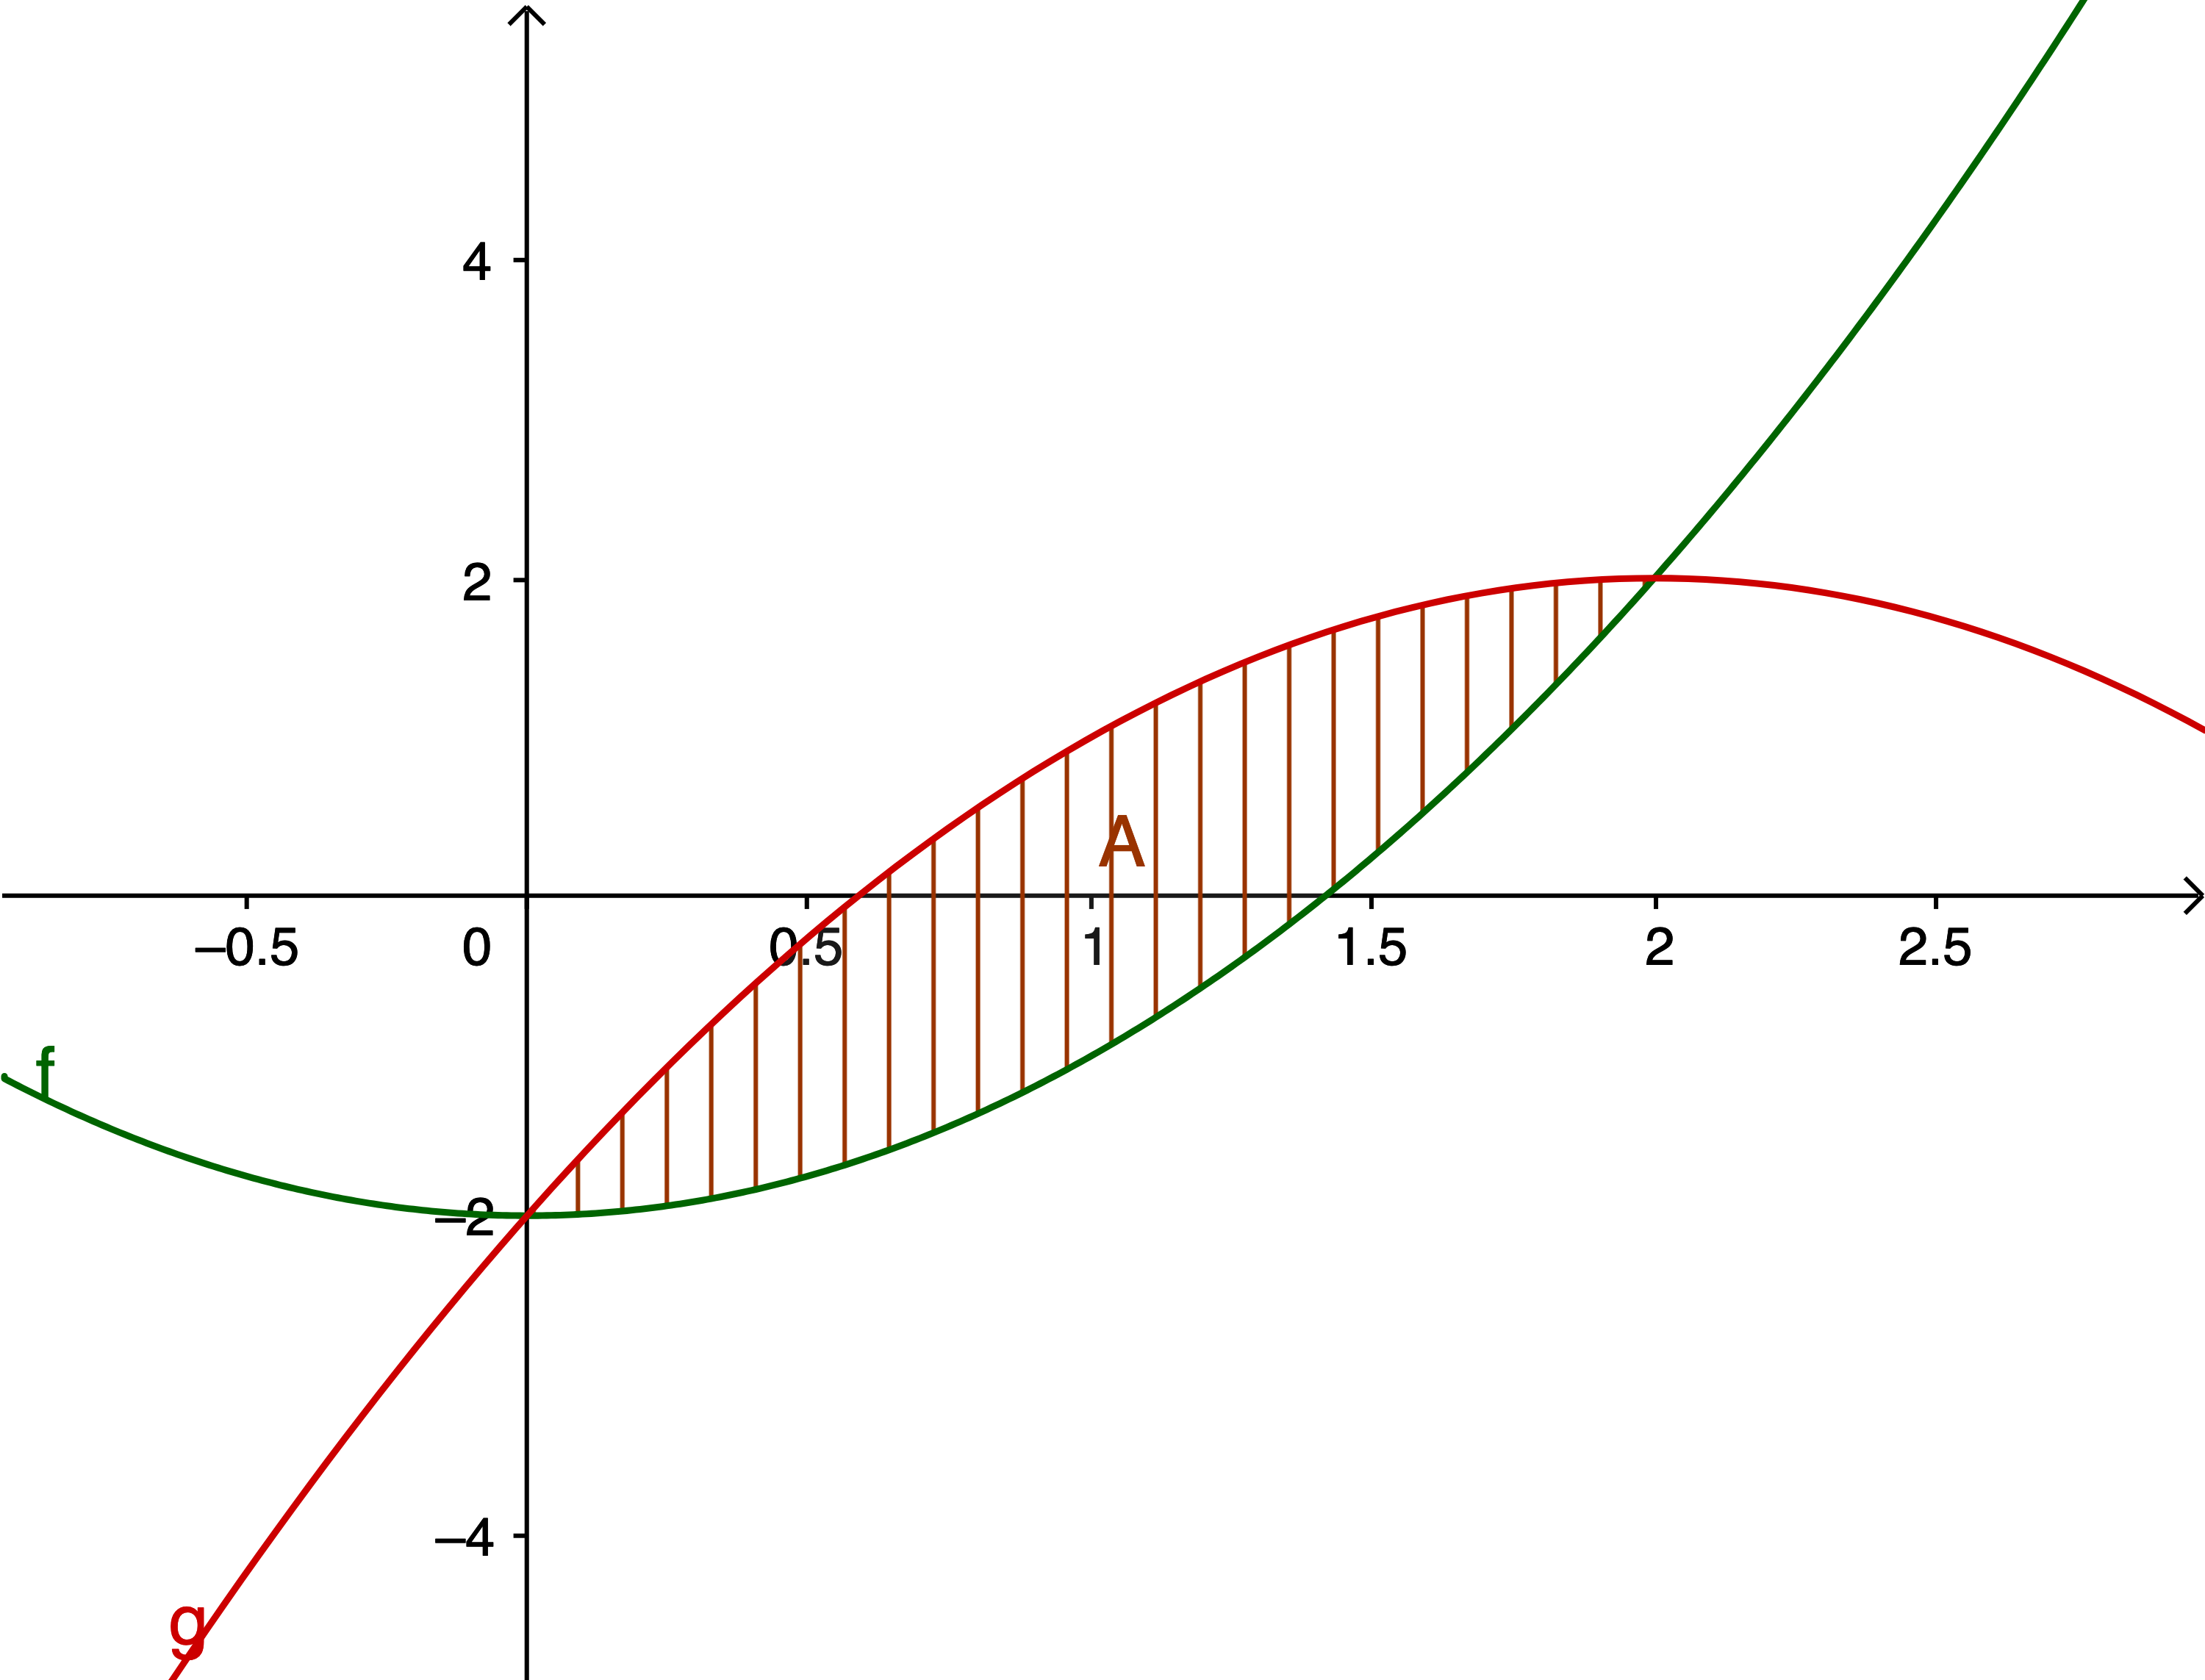
\includegraphics[width = 0.5\textwidth]{media/wal-lebend.png}
	\end{center}
	Die Fläche steht für den lebenden Wal, der durch die Ozeane schwebt. In dieser Lage liegt die Berechnung des Flächeninhalts nicht auf der Hand. Aber es wird einfacher, wenn wir den Wal sterben lassen.
	\begin{center}
		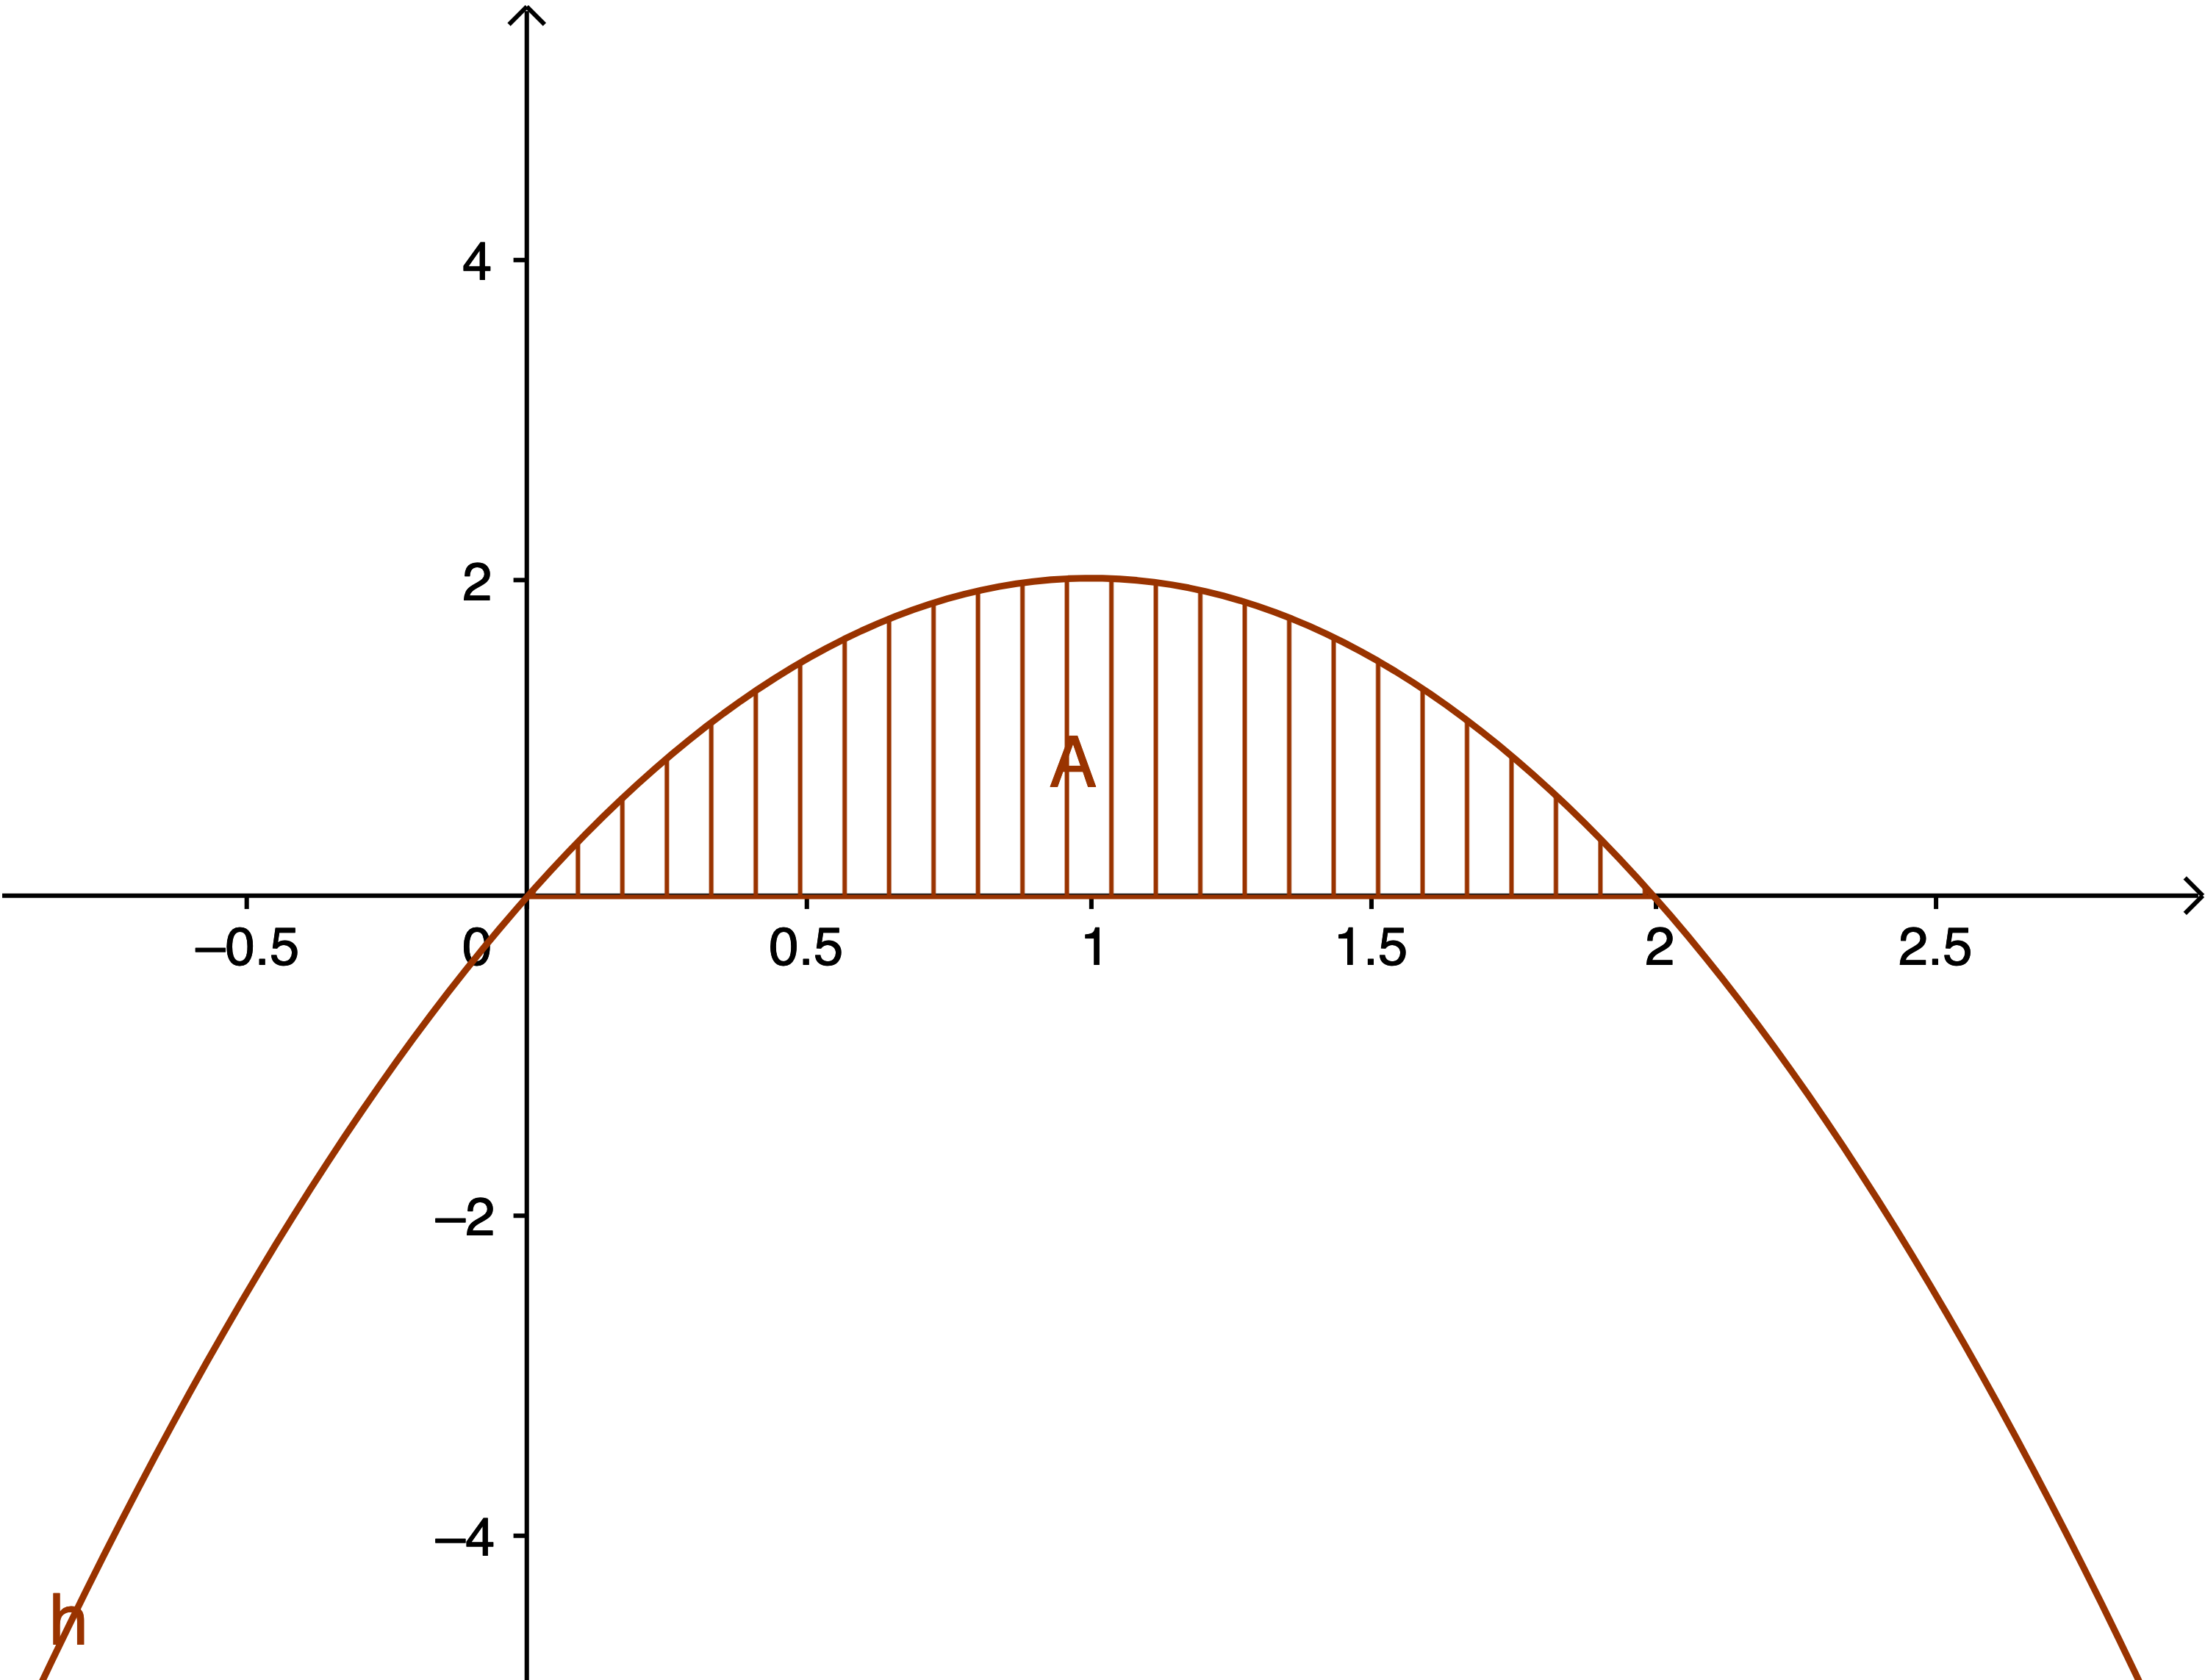
\includegraphics[width = 0.5\textwidth]{media/wal-tot.png}
	\end{center}
	Das ist der tote, gestrandete Wal. Die eingezeichneten Striche sind gleich lang, wie beim lebenden Wal. Die Funktion \(h\), ist demnach definiert durch
	\[ h(x)=g(x)-f(x)=-x^2+4x-2-(x^2-2)=-2x^2+4x \]
	Der Flächeninhalt ist unverändert und es gilt
	\[ A=\int_0^2 (g(x)-f(x))\, dx=\int_0^2 (-2x^2+4x) \, dx=\left[-\frac{2}{3} x^3+2x^2 \right]_0^2=-\frac{2}{3}\cdot 2^3+2\cdot 2^2-0=\frac{8}{3}  \]

\end{bsp}
\begin{satz}
	{Fläche zwischen zwei Graphen}{}

	Seien \(f\) und \(g\) zwei Funktionen, die sich an den Stellen \(x=a\) und \(x=b\) schneiden. Ferner sei \(f(x)\ge g(x)\) für alle \(x\in [a,b]\), das heisst, \(f\) ist die \glqq obere Funktion\grqq{}, \(g\) die \glqq untere Funktion\grqq{}. Dann gilt für den Inhalt der Fläche zwischen den beiden Graphen:
	\[ A=\int_a^b(f(x)-g(x))\, dx \]
	\begin{center}
		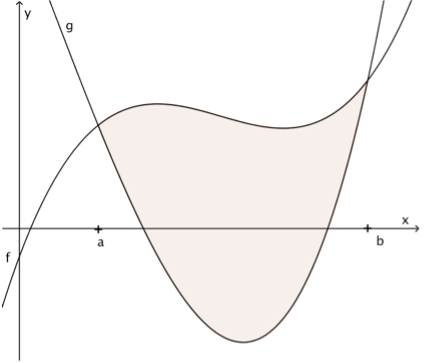
\includegraphics[width = 0.25\textwidth]{media/toterWalBild.png}
	\end{center}

\end{satz}
\begin{proof}
	Betrachten wir zunächst den Fall, wenn beide Kurven über der \(x\)-Achse verlaufen. Dann gilt:
	\begin{figure}[!htb]
		\centering
		\minipage{0.25\textwidth}
		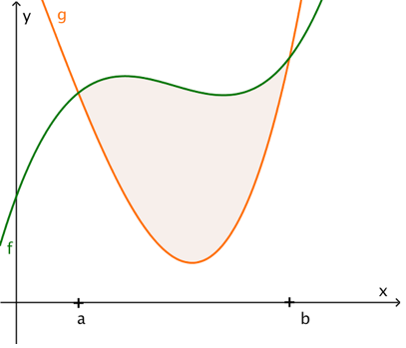
\includegraphics[width=\linewidth]{media/toterWalBew1.png}
		\endminipage \(=\)
		\minipage{0.25\textwidth}
		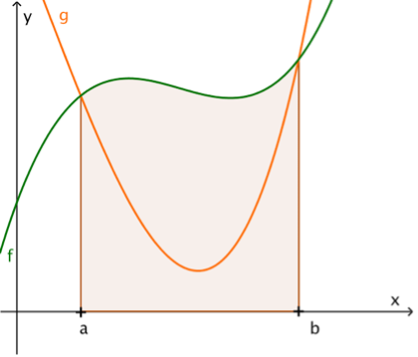
\includegraphics[width=\linewidth]{media/toterWalBew2.png}
		\endminipage \(-\)
		\minipage{0.25\textwidth}
		\includegraphics[width=\linewidth]{media/toterWalBew3.png}
		\endminipage
	\end{figure}

	In Formeln:
	\[ A=\int_a^b f(x)  \, dx -\int_a^b g(x)  \, dx = \int_a^b (f(x)-g(x)) \,dx \]
	Falls die Graphen teilweise oder ganz unter der \(x\)-Achse liegen, können sie zuerst durch Addition einer entsprechenden Konstante über die \(x\)-Achse verschoben werden. Bei der Differenz \(f(x)-g(x)\) fällt die Konstante wieder raus.

\end{proof}

\clearpage
\begin{bsp}
	{}{}
	Gegeben sind die Funktionen \(f(x)=2x^3-2x^2-4x\) und \(g(x)=-x^3+x^2+2x\). Gesucht ist der Flächeninhalt des endlichen Gebietes, welches durch die beiden Graphen eingeschlossen wird.
	\vspace{20cm}
\end{bsp}
\clearpage
\begin{ueb}
	{Polynomfunktionen}{}
	\begin{enumerate}
		\item Berechnen Sie den Inhalt des Flächenstückes, das die Graphen der Funktionen \(f_1\) und \(f_2\) einschliessen.
		      \begin{enumerate}
			      \item \(f_1: y=x,\qquad f_2: y=x^2\)
			      \item \(f_1: y=x,\qquad f_2: y=x^3\)
			      \item \(f_1: y=2x-3,\qquad f_2: y=x^2-2x-8\)
			      \item \(f_1: y=x^3,\qquad f_2: y=2x-x^2\)
			      \item \(f_1: y=x^2-3x,\qquad f_2: y=x^3-6x^2+9x\)
		      \end{enumerate}
		\item Welchen Inhalt hat das Flächenstück, das zwischen der Parabel \(y=3x-x^2\) und den Tangenten in den beiden Nullstellen der Parabel eingeschlossen wird?
		\item Berechnen Sie den Inhalt der Fläche zwischen dem Graphen \(f(x)= 3x(x^2-3x+2)\) und der Tangenten im Wendepunkt des Graphen und der \(y\)-Achse.
		\item Für welchen Wert von \(a\) schliessen die beiden Graphen der Funktionen \(f(x)=x^2-ax\) und \(g(x)= ax\) eine Fläche mit dem Inhalt \(A=36\) ein?
	\end{enumerate}
\end{ueb}
\begin{ueb}
	{Andere Funktionstypen}{}
	\begin{enumerate}\setcounter{enumi}{4}
		\item Berechnen Sie den Inhalt des Flächenstückes, das die Graphen der Funktionen \(f(x) = 2\sqrt{4-x}\) und \(g(x)=x^2-5x+4\) einschliessen.

		\item Berechnen Sie den Inhalt einer der (unendlich vielen) Flächenstücke, die zwischen der Graphen \(f(x)=\sin(x)\) und \(g(x)=1-\sin(x)\) liegen.
		\item Berechnen Sie den Inhalt einer der (unendlich vielen) Flächenstücke, die zwischen der Graphen \(f(x)=\sin(x)\) und \(g(x)=\sqrt{3}\cos(x)\) liegen.
		\item Berechnen Sie den Inhalt der Fläche zwischen den Graphen von \(f(x)=\frac{1}{x}\) und \(g(x) = \frac{2}{x}\) im Intervall \(x\in [1, 3]\).
	\end{enumerate}
\end{ueb}

\clearpage

\emph{Lösungen:}
\begin{enumerate}
	\item Flächen zwischen Polynomfunktionen:
	      \begin{enumerate}
		      \item \(A=\frac{1}{6}\)
		      \item \(A=\frac{1}{2}\)
		      \item \(A= 36\)
		      \item \(A= \frac{37}{12}\)
		      \item \(A=11.83\bar{3}\)
	      \end{enumerate}
	\item \(A=2.25\)
	\item \(A=\frac{3}{4}\)
	\item \(a=\pm3\)
	\item \(A=13.33\bar{3}\)
	\item Schnittstellen: \(x_1= \frac{\pi}{6}\), \(x_2= \frac{5\pi}{6}\), Flächeninhalt \(A=2\sqrt{3}-\frac{2\pi}{3}\)
	\item Schnittstellen: \(x_1= \frac{\pi}{3}\), \(x_2= \frac{4\pi}{3}\), Flächeninhalt \(A=4\)
	\item \(A= \ln(3)\)
\end{enumerate}









































\clearpage
\subsubsection{Volumen}
\begin{LA}
	{Das Volumen der Pyramide}{}
	Wie sie wissen, lautet die Formel zur Berechnung des Volumens einer Pyramide \(V=\frac{1}{3} Gh\). Diese Formel wurde zwar schon etwa 400 v.Chr. von Demokrit entdeckt, der Beweis für ihre Richtigkeit ist aber nicht einfach. Eine Methode, welche schon im Altertum angewendet wurde, besteht darin, die Pyramide durch einen Stapel dünner, quaderförmigen Scheiben anzunähern.
	\begin{center}
		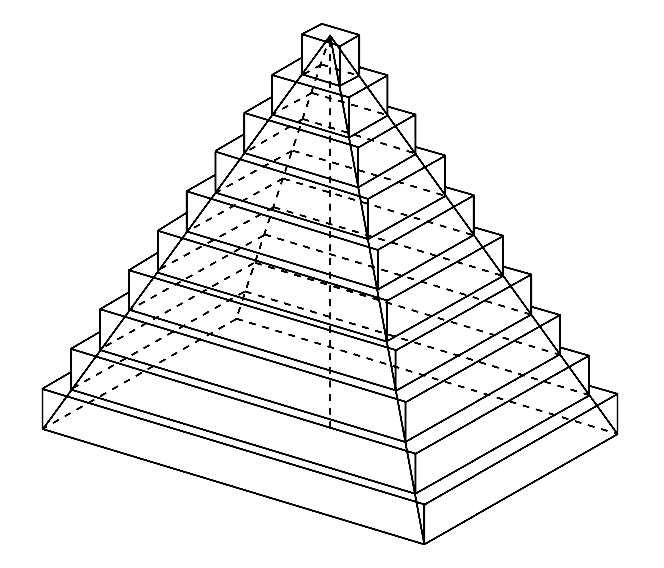
\includegraphics[width = 0.5\textwidth]{media/pyramideInScheiben.png}
	\end{center}

	Der Einfachheit halber betrachten wir eine gerade, vierseitige Pyramide. Damit wir die Volumina der einzelnen Quader im Bild oben berechnen können, benötigen wir eine Formel für den Flächeninhalt \(A(x)\) einer parallel zur Grundfläche liegenden Schnittfläche durch die Pyramide im Abstand \(x\) von der Spitze der Pyramide.
	\begin{center}
		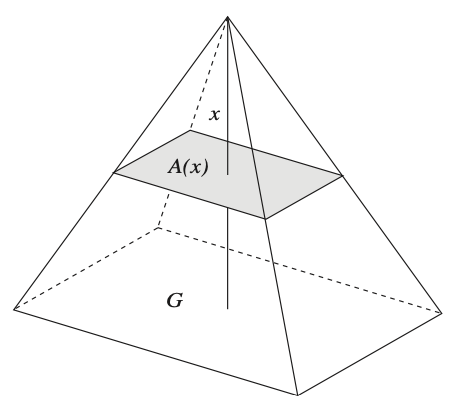
\includegraphics[width = 0.5\textwidth]{media/pyramideMitQuerschnit.png}
	\end{center}
	Die Pyramide mit der Grundfläche \(G\) und der Höhe \(h\) ist ähnlich zu jener mit Grundfläche \(A(x)\) und Höhe \(h\). Daraus ergibt sich:
	\[\frac{A(x)}{G} = \left(\frac{x}{h}\right)^2 \Longrightarrow A(x)=\frac{G}{h^2}\cdot x^2 \]

	\begin{enumerate}
		\item 	Angenommen die Pyramide wird durch vier Quadern angenähert. Wie lautet dann das approximative Volumen in Abhängigkeit von \(G\) und \(h\)?
		      (Kontrolle: \(V\approx \frac{15}{32} Gh\) )
		\item Die in der Skizze verwendeten Quader sind alle ein wenig zu gross. Wie lautet eine entsprechende Annäherung durch 4 Quadern, die alle im Inneren der Pyramide liegen und damit ein wenig zu klein sind? (Beachten Sie, dass der oberste der vier Quader dann das Volumen 0 hat.)
		      (Kontrolle: \(V\approx \frac{7}{32} Gh\) )
		\item Betrachten Sie nun den Graphen der Funktion \(A(x)=\frac{G}{h^2}\cdot x^2\) im Intervall \([0,h]\) (unten) und berechnen Sie den Wert der Untersumme \(U_4\).
		      \begin{center}
			      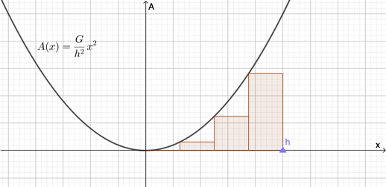
\includegraphics[width = 0.5\textwidth]{media/graphZurPyramide.png}
		      \end{center}
		\item Vergleichen Sie Ihre Rechnungen für die Aufgaben 2. und 3. Was stellen Sie fest? Was folgt daraus für die Berechnung des exakten Volumens einer Pyramide.
	\end{enumerate}

\end{LA}
\clearpage
Mit bestimmten Integralen können nicht bloss Flächeninhalte berechnet werden, sondern auch Volumina von Körpern:
\begin{satz}
	{Merksatz}{}
	Das Volumen eines Körpers ist das Integral über die Querschnittsfläche.
	\begin{center}
		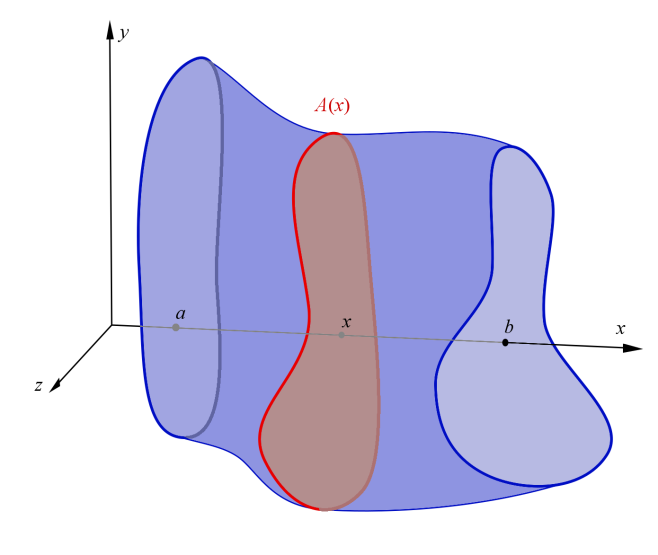
\includegraphics[width = 0.5\textwidth]{media/querschnitt.png}
	\end{center}
	\[ V = \int_a^b A(x) \, dx\]
\end{satz}
Besonders einfach ist damit die Berechnung von Volumina von Körpern, die durch Rotation eines Graphen um die \(x\)-Achse entstehen. Das folgende Beispiel soll dies veranschaulichen.
\begin{bsp}
	{Rotationsvolumen}{}
	Betrachten Sie die Kurve \(y=\sqrt x\) im Intervall \(x\in[0,1]\). Wird diese Kurve um die \(x\)-Achse gedreht, so entsteht ein sogenanntes Paraboloid:
	\begin{center}
		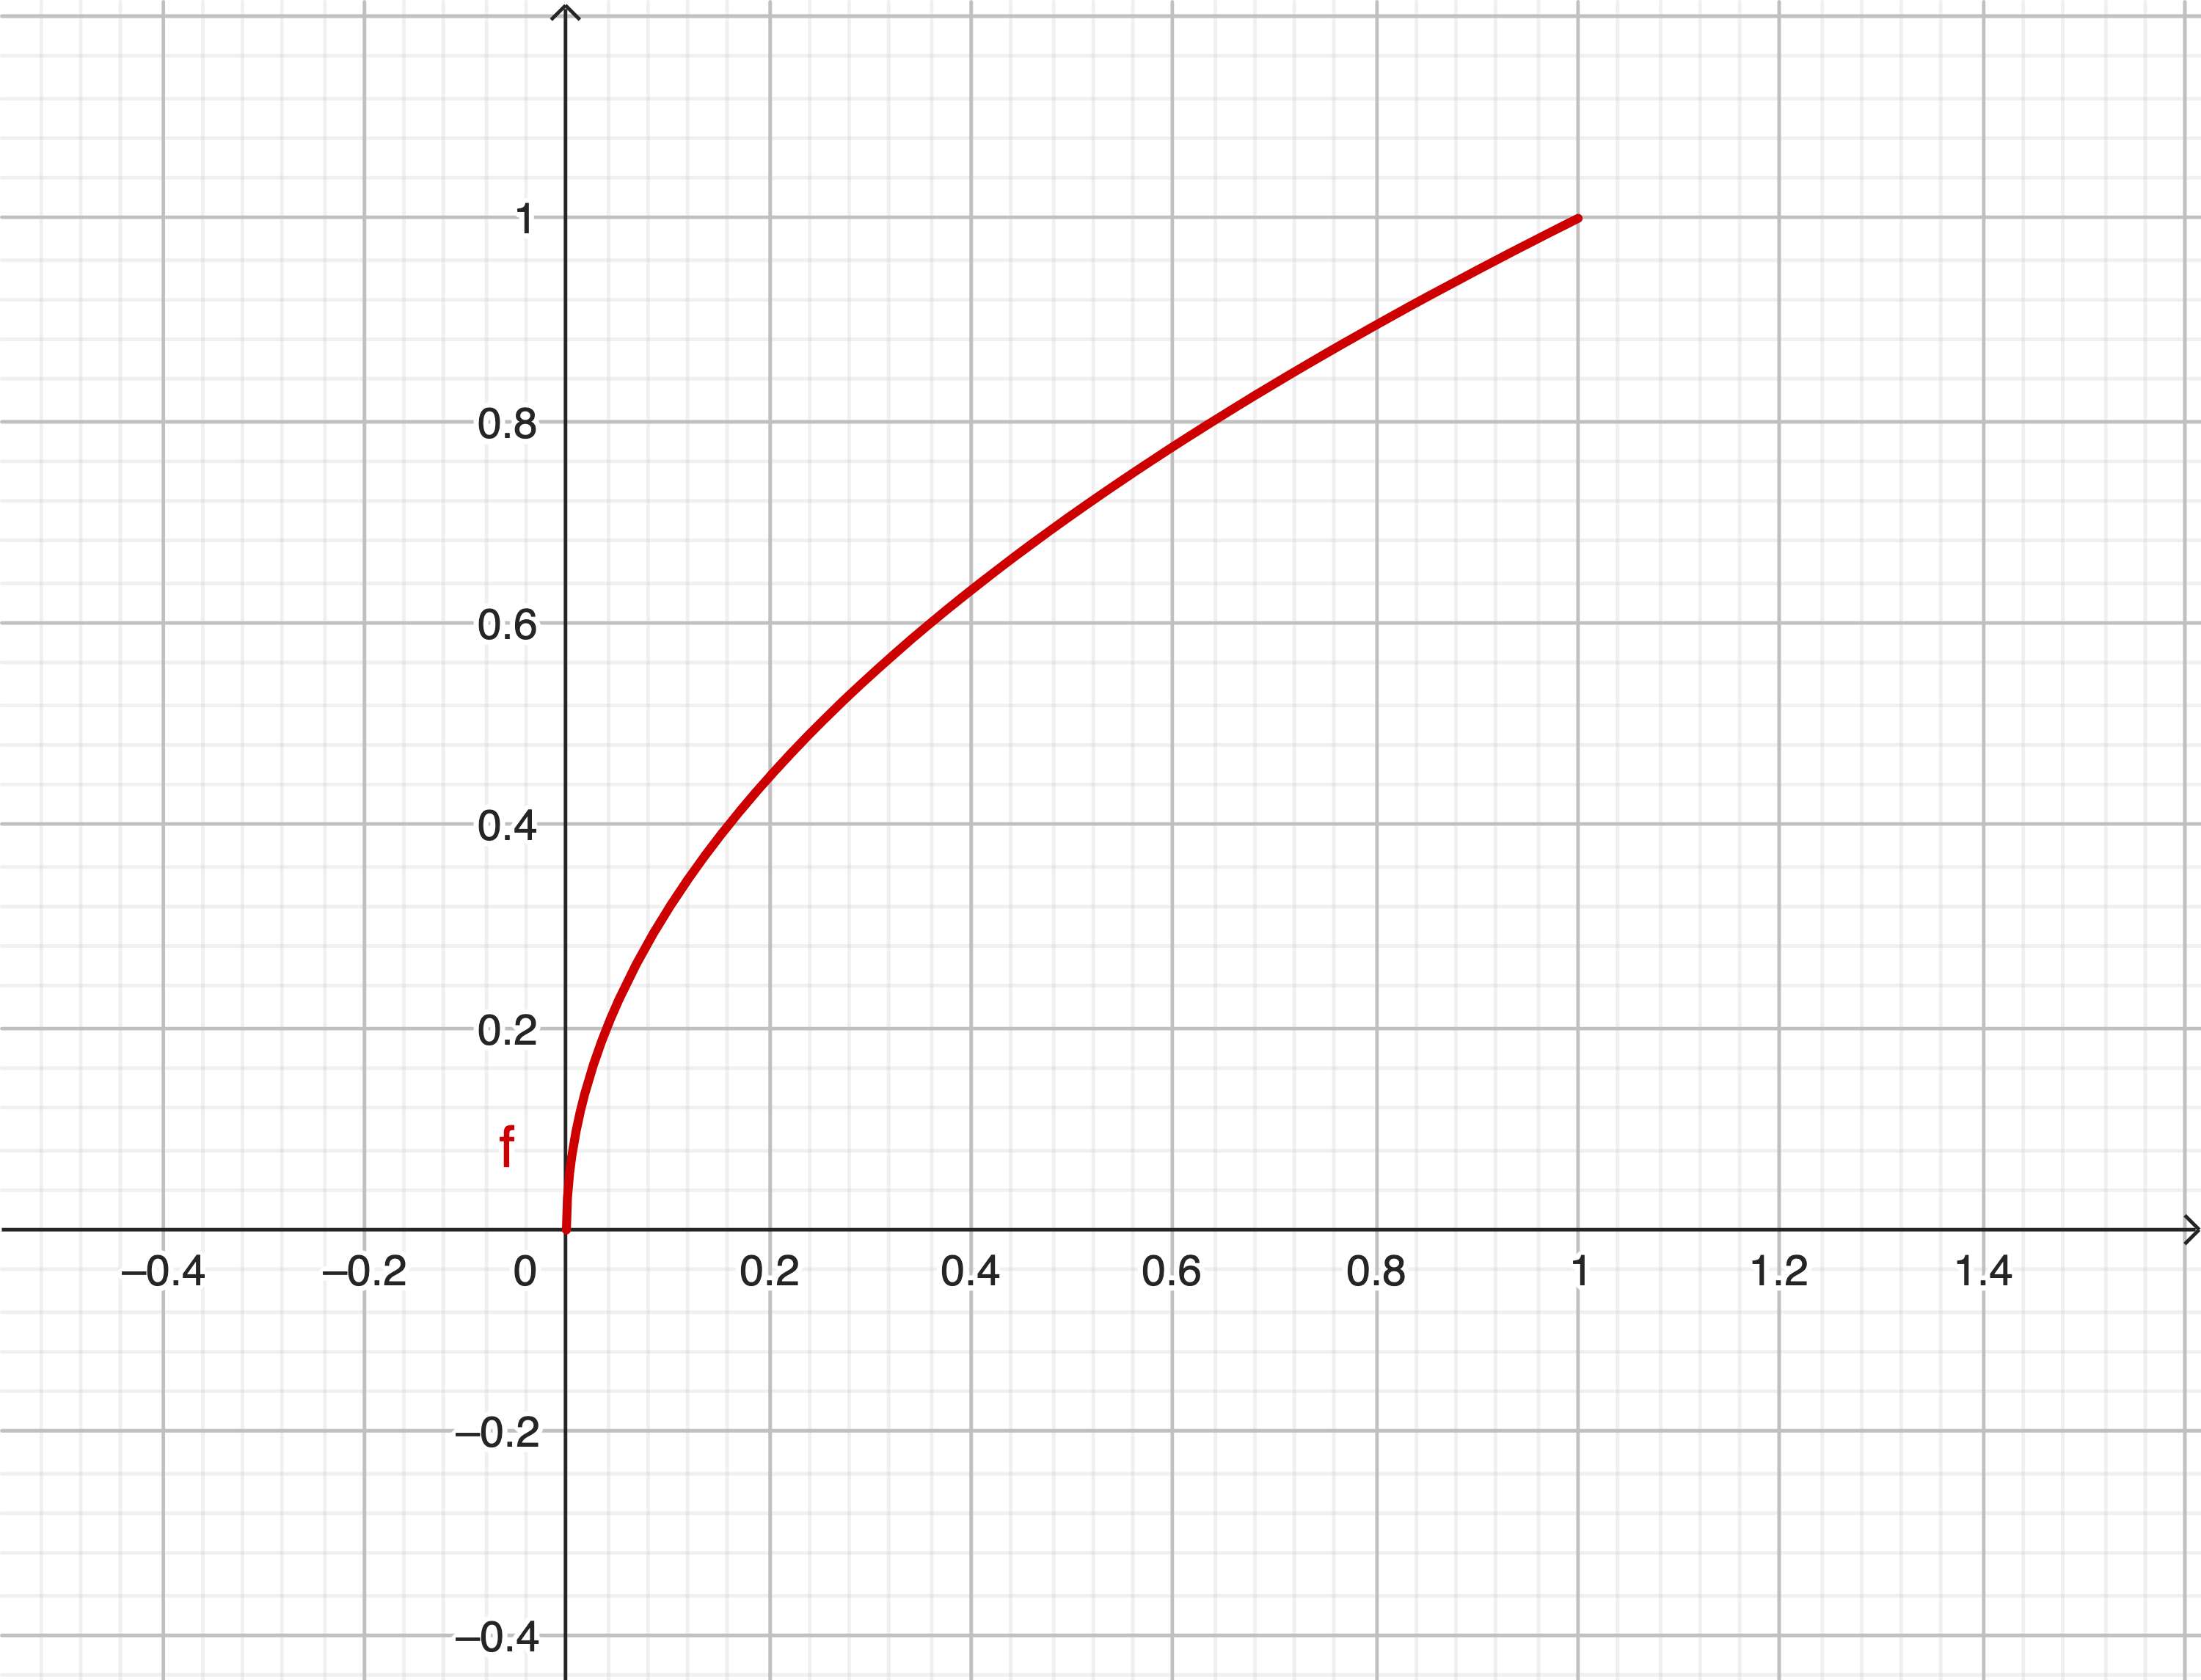
\includegraphics[width = 0.4\textwidth]{media/IntroRotationsVolumen2dv2.png}\hfill
		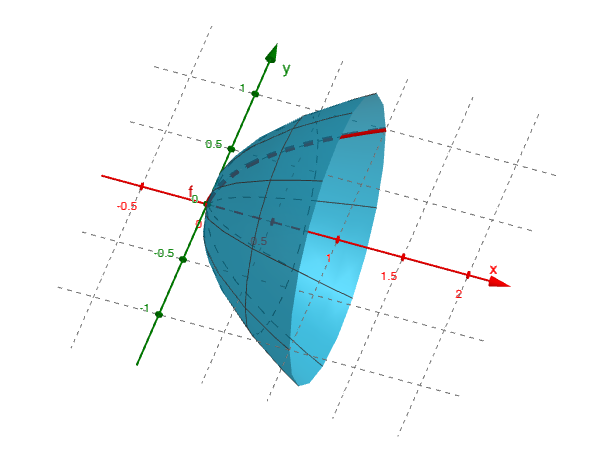
\includegraphics[width = 0.4\textwidth]{media/IntroRotationsVolumen3dv2.png}
	\end{center}

	% \begin{figure}[!htb]
	%     \minipage{0.4\textwidth}
	%       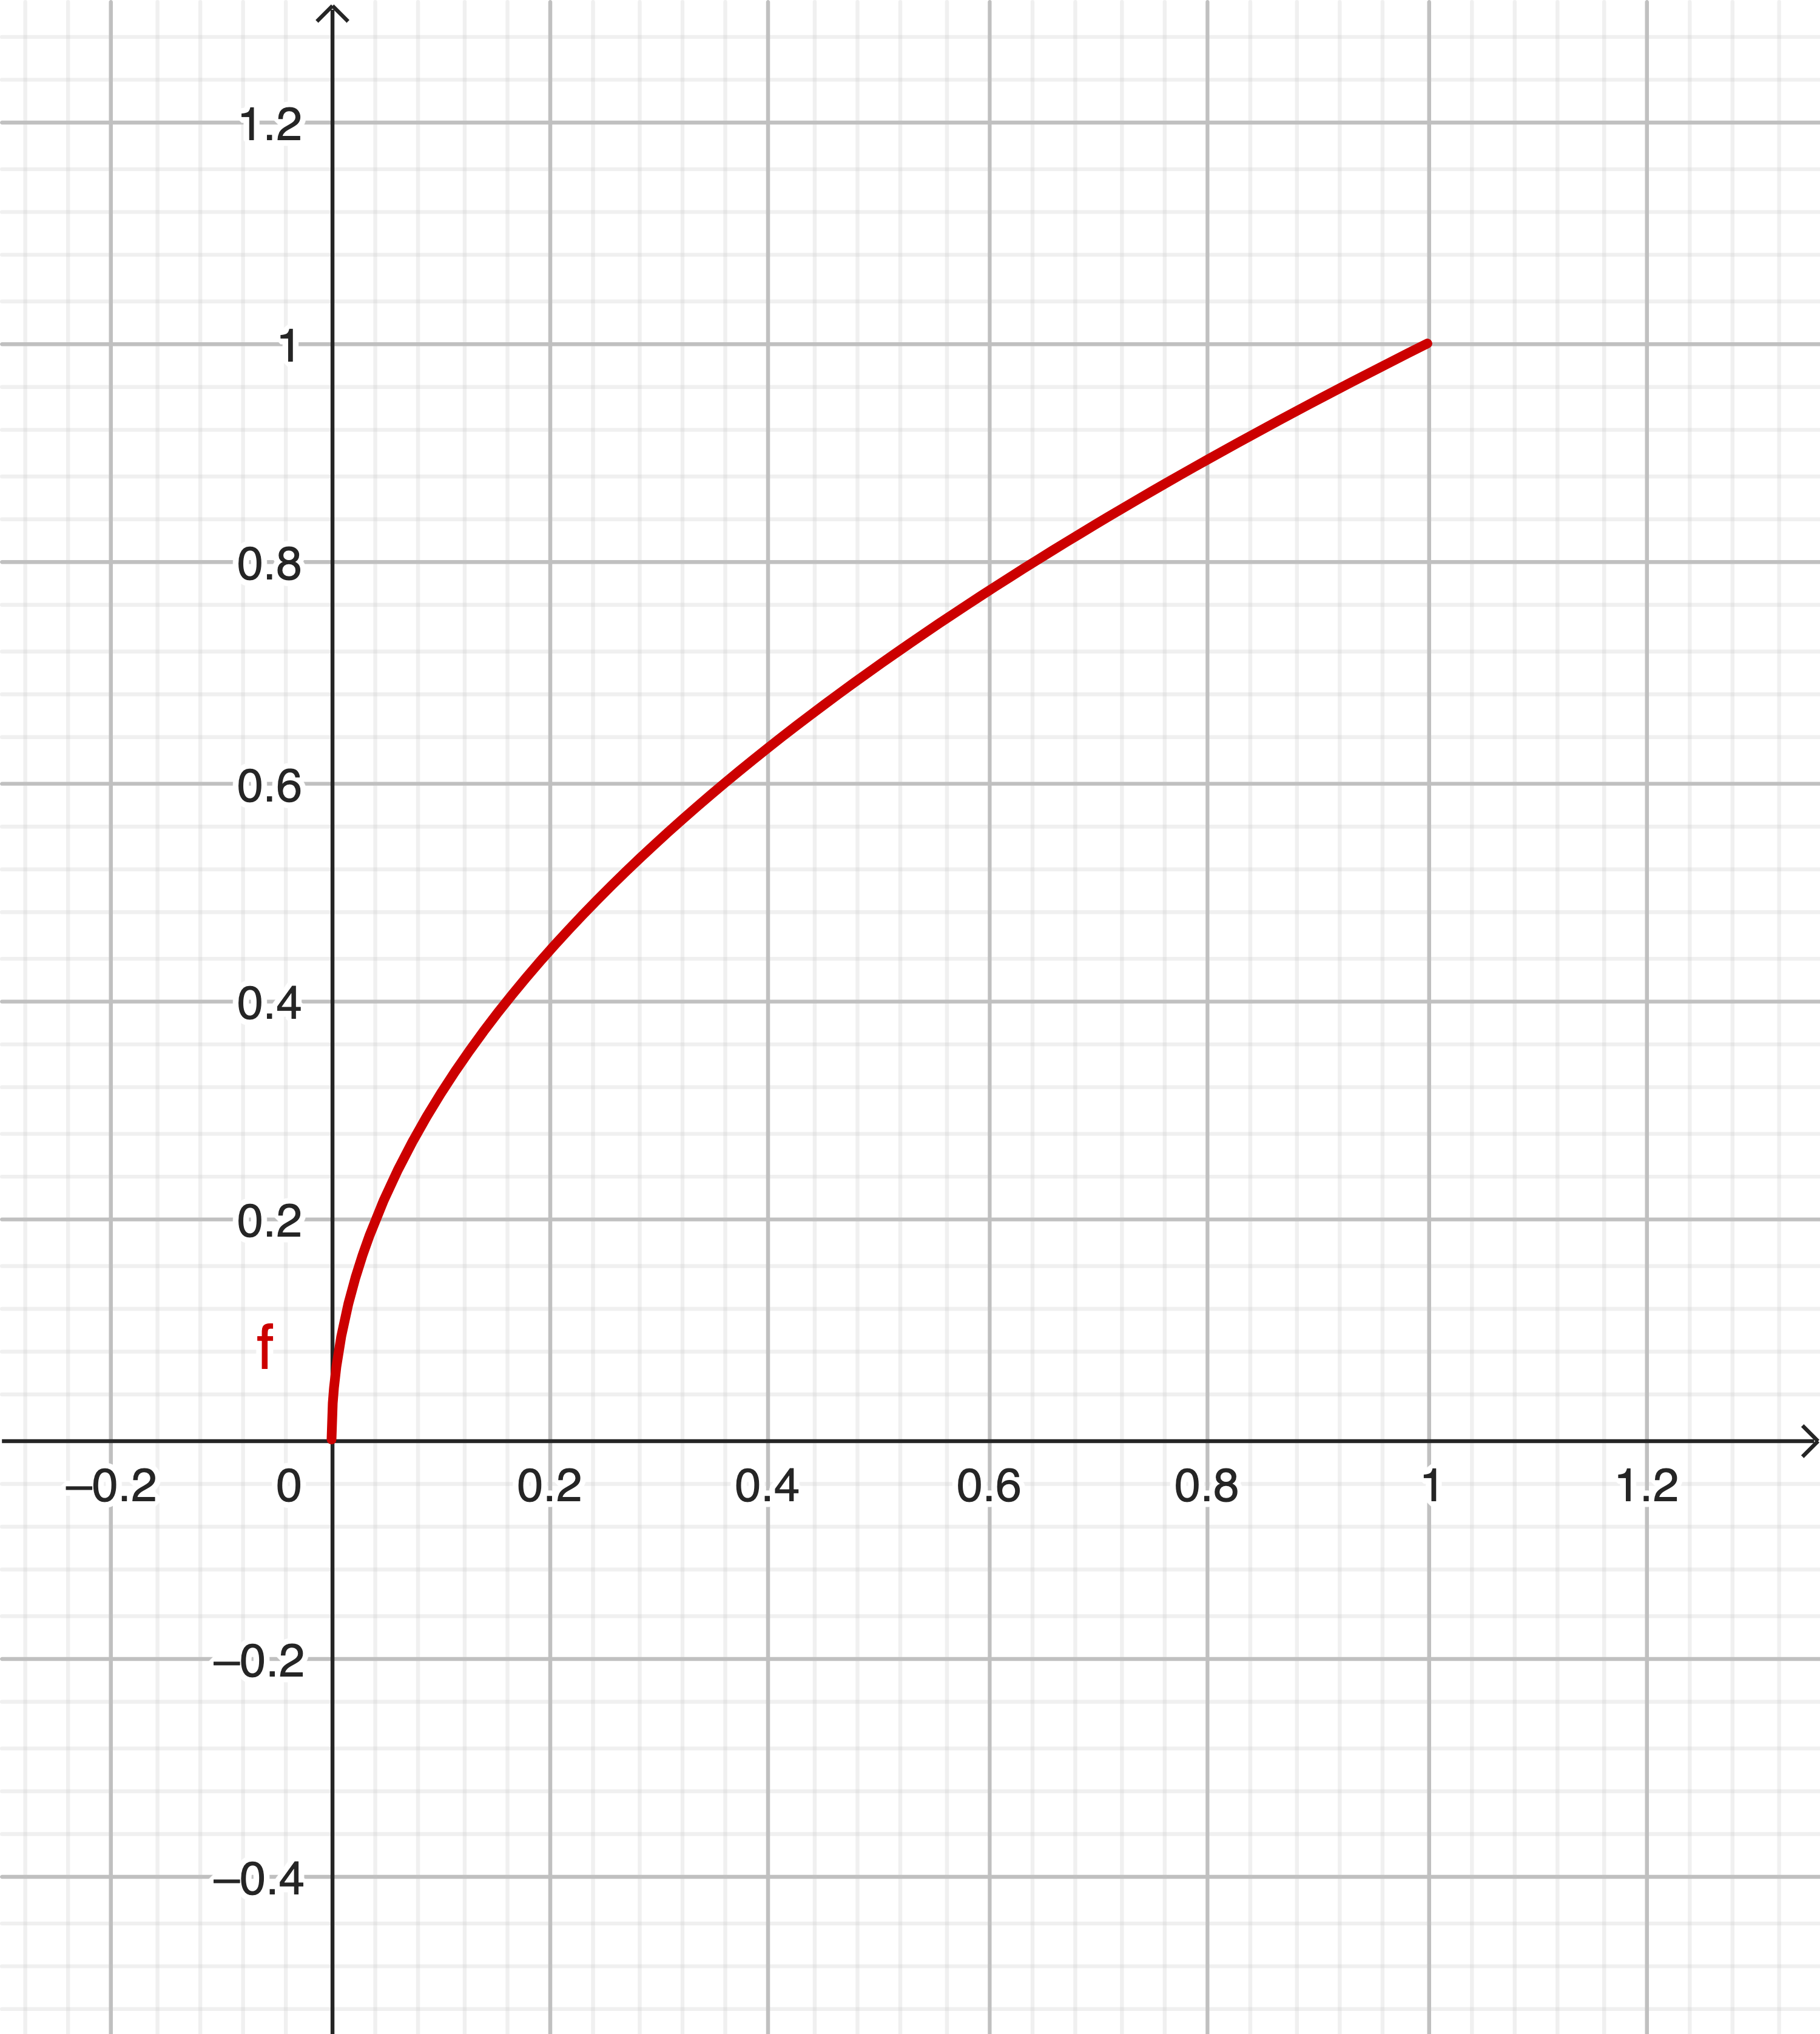
\includegraphics[width=\linewidth]{media/IntroRotationsVolumen2D.png}
	%     \endminipage\hfill
	%     \minipage{0.4\textwidth}
	%       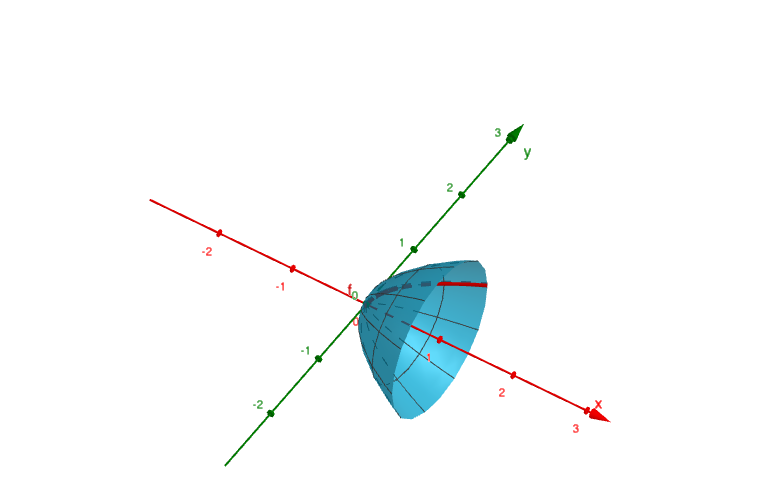
\includegraphics[width=\linewidth]{media/IntroRotationsVolumen3D.png}
	%     \endminipage
	% \end{figure}

	Die Querschnittsflächen des Paraboloids, die senkrecht zur \(x\)-Achse stehen, sind Kreise mit dem Radius \(y=\sqrt x\). Der Flächeninhalt dieser Kreise ist demnach \(A(x)=\pi y^2=\pi (\sqrt x)^2=\pi x\). Das Volumen des Paraboloids beträgt damit
	\[V=\int_0^1 \pi y^2 \, dx =\int_0^1\pi x \, dx=\left[\frac{\pi}{2} x^2 \right]_0^1= \frac{\pi}{2}\cdot 1^2-\frac{\pi}{2}\cdot 0^2=\frac{\pi}{2}\]

\end{bsp}
Allgemein gilt:
\begin{satz}
	{Rotationsvolumen}{}
	Wird eine Kurve \(y=f(x)\) im Intervall \([a,b]\) um die \(x\)-Achse gedreht, entsteht ein Körper mit dem Volumen
	\[V=\int_a^b \pi \cdot (f(x))^2 dx\]

\end{satz}


\textbf{Bemerkung}: Da \(\pi\) ein konstanter Faktor ist, kann man ihn auch vor das Integral stellen.
\[V=\pi \cdot\int_a^b  (f(x))^2 dx\]

\begin{bsp}{}{}
	Die endliche Fläche zwischen der \(x\)-Achse und der Kurve \(y=4-x^2\) rotiert um die \(x\)-Achse. Bestimmen Sie das Volumen des Rotationskörpers?
	\begin{center}
		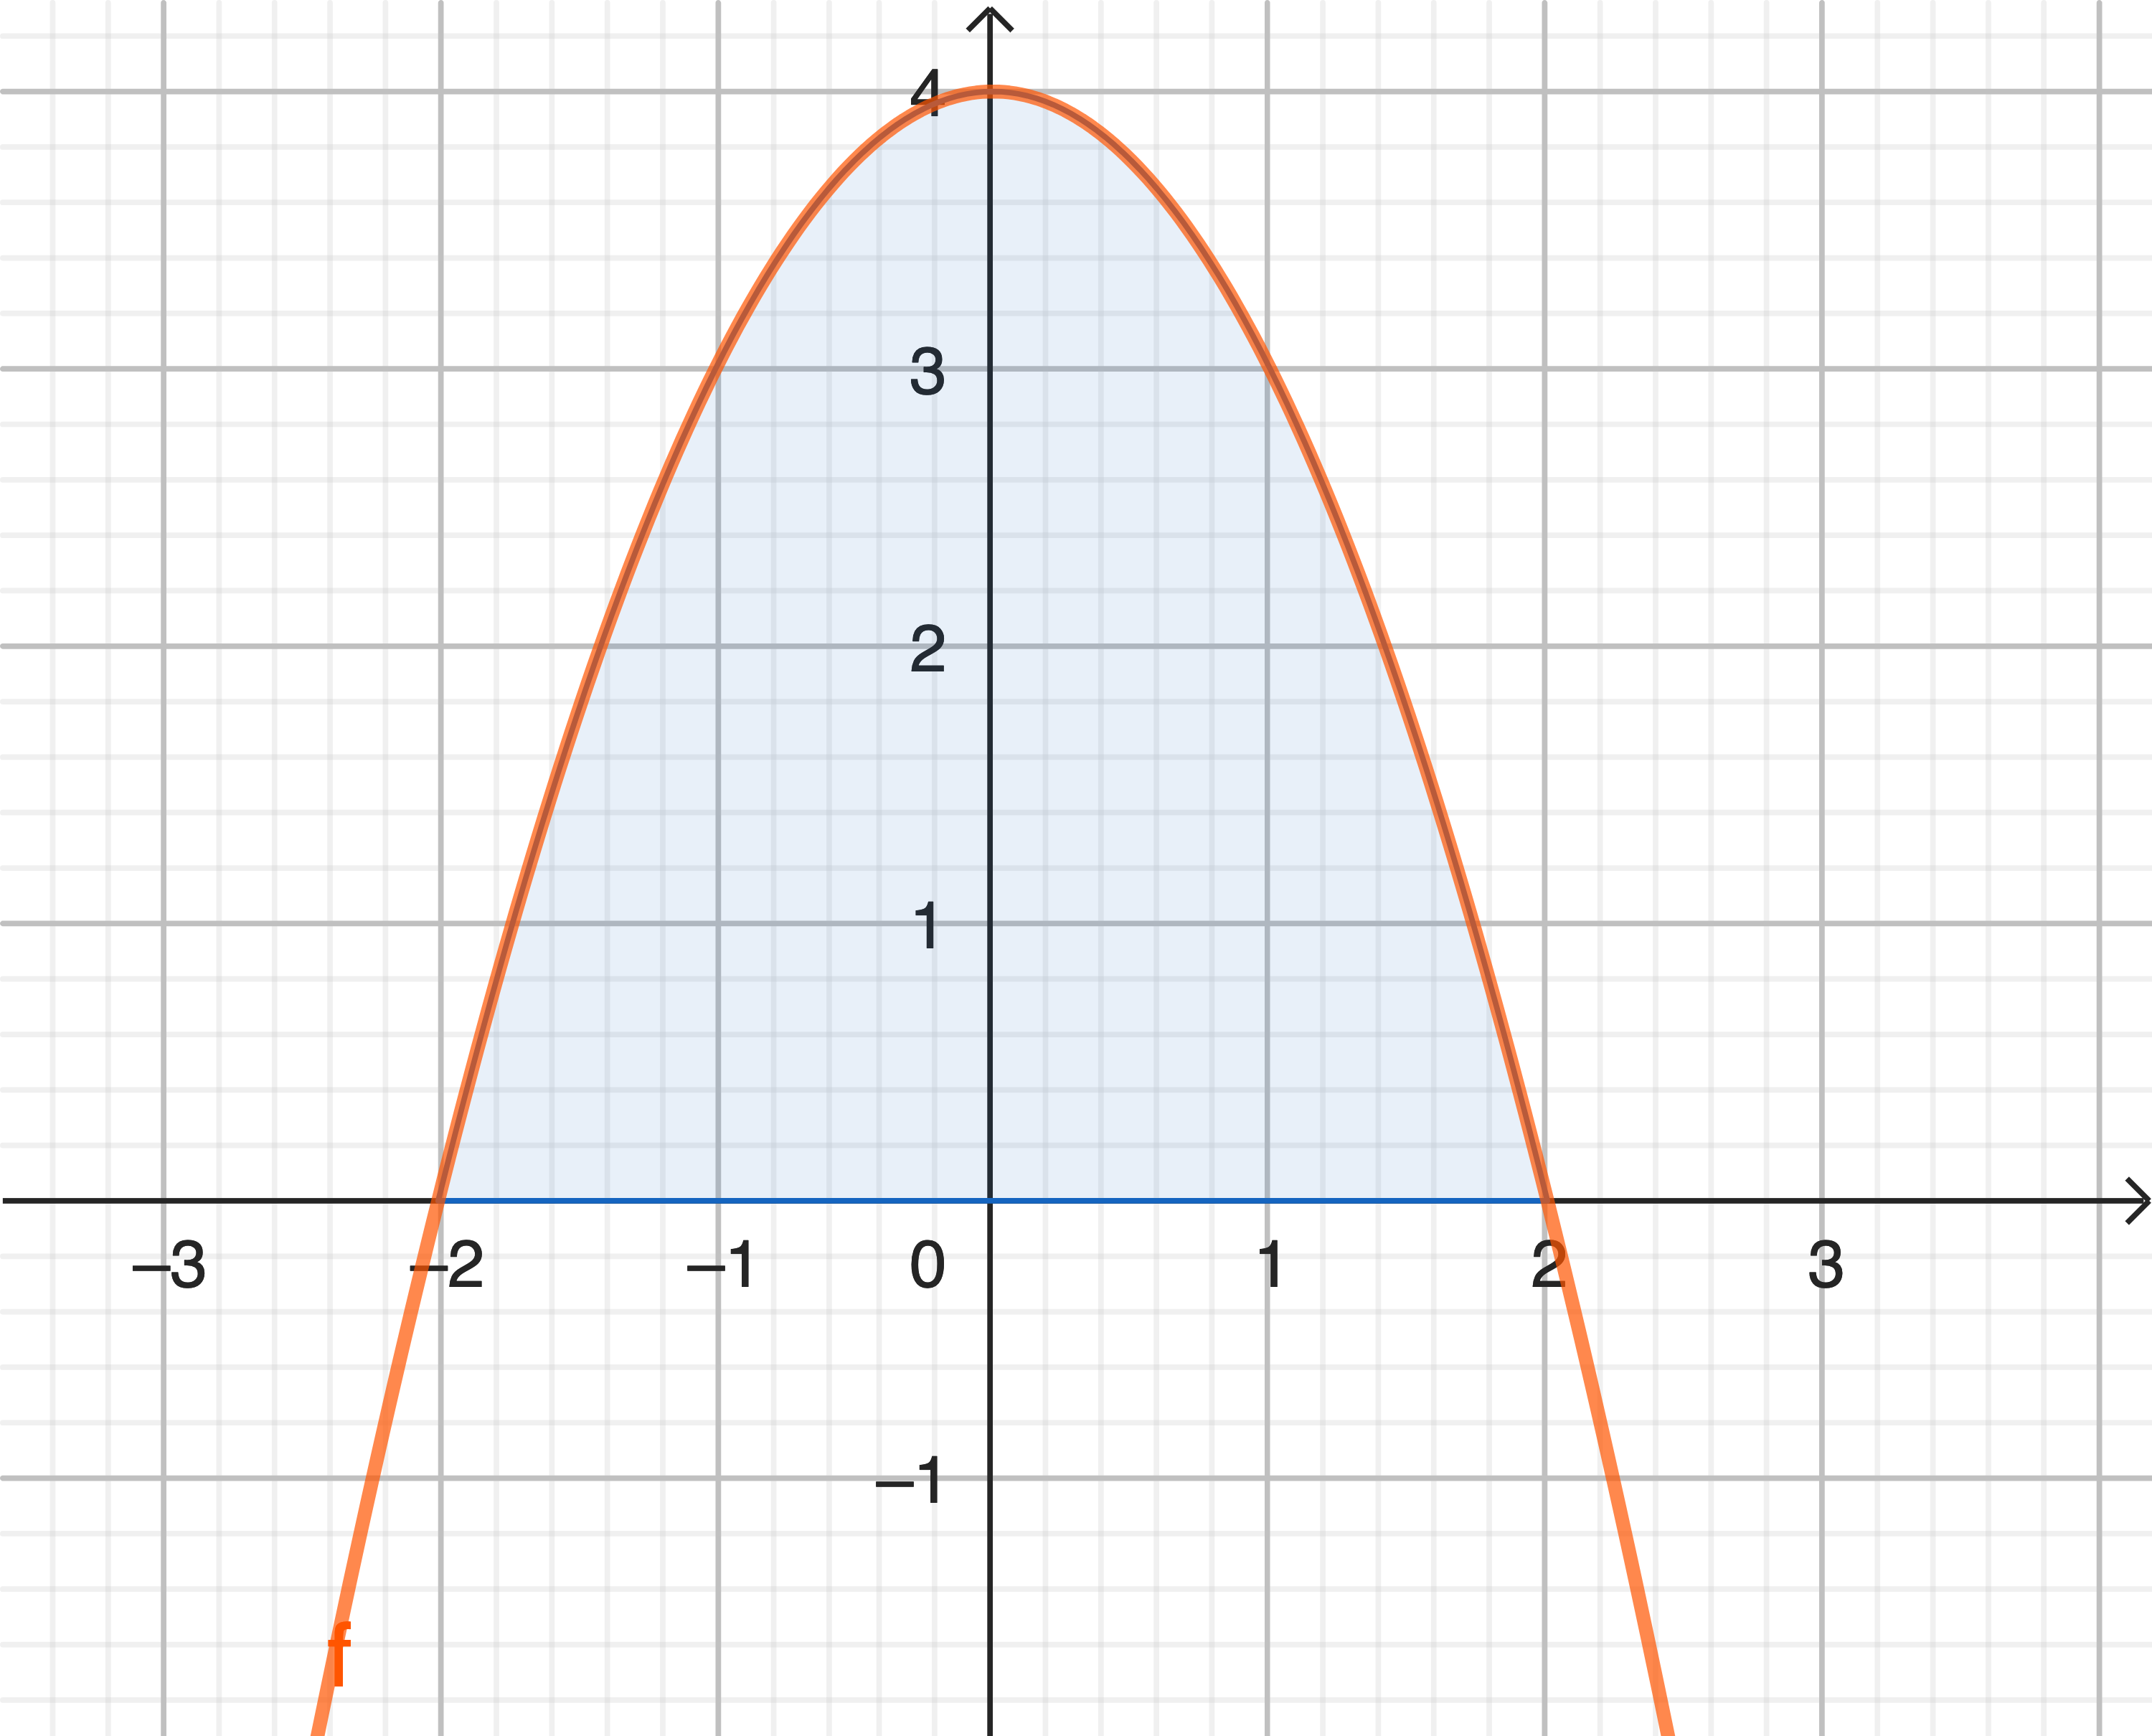
\includegraphics[width = 0.5\textwidth]{media/rotationsVolumenBsp2.png}
	\end{center}

	\vspace*{6cm}
	% Die Fläche zwischen Kurve und $x$-Achse wird durch die Nullstellen der Kurve begrenzt. Diese sind:
	% $$4-x^2=0 \iff 4=x^2 \iff x_{1,2}=\pm 2$$
	% Damit gilt für das Volumen des Rotationskörpers
	% $$ V=\pi \cdot \int_{-2}^2 (4-x^2)^2 \, dx =\pi \cdot \int_{-2}^2 (16-8x^2+x^4 )  \, dx =\pi \cdot \left[16x-\frac{8}{3} x^3+\frac{1}{5} x^5 \right]_{-2}^2=\frac{160}{3} \pi $$ 

\end{bsp}

\clearpage
\begin{ueb}
	{}{}
	\begin{enumerate}
		\item Die endliche Fläche zwischen der gegeben Kurve und der \(x\)-Achse rotiert um die \(x\)-Achse. Berechnen Sie das Volumen der Rotationskörpers.
		      \begin{enumerate}
			      \item \(y=2x-x^2\)
			      \item \(y=x^3-3x^2\)
			      \item \(y=\sqrt{1-x^2}\)
		      \end{enumerate}
		\item Die Fläche zwischen den beiden Kurven rotiert um die \(x\)-Achse. Berechnen Sie das Volumen des Rotationskörpers.
		      \begin{enumerate}
			      \item \(y=x\) und \(y=x^3\)
			      \item \(y=x^2+3\) und \(y=-2x^2+6\)
		      \end{enumerate}
		\item Die Kurve \(y=\frac{1}{4}x^3\) und die Kurventangente im Punkt \(P=(2, y_P)\) begrenzen im 1. Quadranten eine Fläche, die um die \(x\)-Achse rotiert wird. Berechnen Sie das Volumen des Rotationskörpers.
		\item Challenge: Perlenkette
		      \begin{enumerate}
			      \item Zeigen Sie, dass \(F(x)=\frac{1}{2}\left(x-\sin(x) \cdot \cos(x)\right)\) eine Stammfunktion der Funktion \(f(x) = \sin^2(x)\) ist. Benutzen Sie dazu den trigonometrischen Pythagoras.
			      \item   Wenn die Sinuskurve um die \(x\)-Achse rotiert, ensteht eine Art unendliche Perlenkette. Berechnen Sie das Volumen eines der Glieder dier Kette.
		      \end{enumerate}

	\end{enumerate}


\end{ueb}

\clearpage
\emph{Lösungen:}
\begin{enumerate}
	\item Rotationsvolumen:
	      \begin{enumerate}
		      \item \(V=\frac{16}{15}\pi\)
		      \item \(V=\frac{729}{35}\pi\)
		      \item \(V=\frac{4}{3}\pi\) (Der Körper ist eine Kugel mit Radius 1!)
	      \end{enumerate}
	\item Rotationsvolumen zwischen zwei Kurven:
	      \begin{enumerate}
		      \item \(V=\frac{8}{21}\pi\)
		      \item \(V\approx 110.58\)
	      \end{enumerate}
	\item \(V=\frac{16}{63}\pi\)
	\item Perlenkette:
	      \begin{enumerate}
		      \item Mit der Produktregel ableiten und mit dem trigonometrischen Pythagoras \(1-\cos^2(x)=\sin^2(x)\) vereinfachen.
		      \item \(V=\frac{\pi^2}{2}\)
	      \end{enumerate}

\end{enumerate}

\clearpage
\subsubsection*{Volumen als Integral der Querschnittsfläche}
In diesem Abschnitt werden Sie Volumen von Körpern berechnen, die nicht aus der Rotation um eine Achse entstanden sind. Diese Volumina können als Integrale der entsprechenden Querschnittsflächen berechnet werden:
\[ V= \int_{a}^{b} A(x) dx\]

\begin{ueb}
	{Das Volumen der Quarterpipe}{quarterpipe}
	Um das Volumen einer Quarterpipe zu berechnen, wird diese in ein Koordinatensystem eingebettet. Dabei modellieren wir die Quarterpipe als einen Körper, der dadurch ensteht, dass man die Parabel \(y=\frac{1}{20} x^2\) senkrecht zur \(xy\)-Ebene verschiebt. Den Körper approximieren wir durch dünne Quader, deren Grundfläche Querschnitte der Quarterpipe sind.
	\begin{center}
		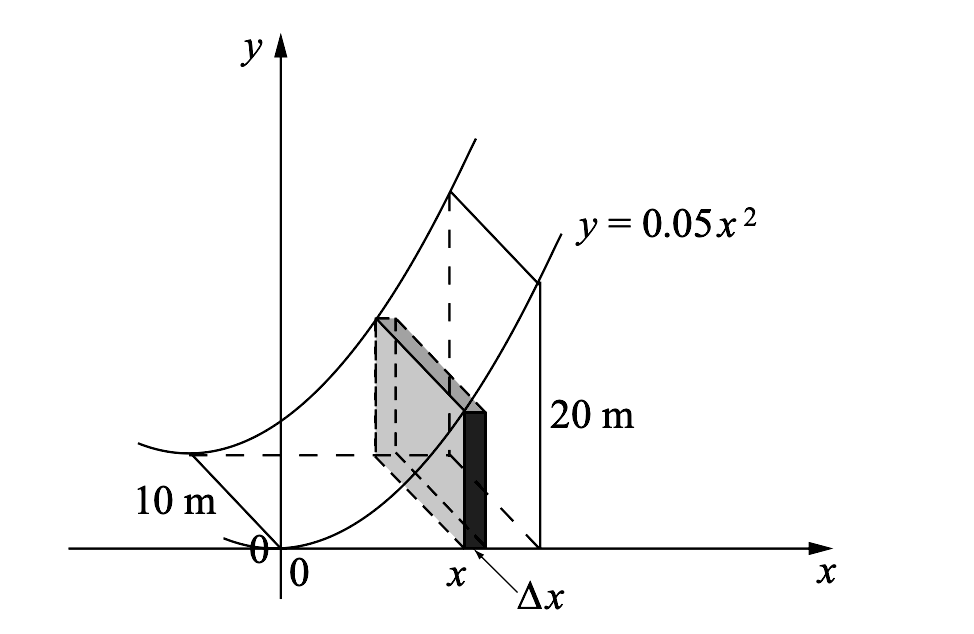
\includegraphics[width = 0.5 \textwidth]{media/quarterpipe.png}
	\end{center}
	\begin{enumerate}
		\item Berechnen Sie den Flächeninhalt \(A(x)\) eines Querschnitts der Quarterpipe im Abstand \(x\) vom Ursprung.
		\item Berechnen Sie das Volumen der Quarterpipe, indem Sie die Querschnittsfläche integrieren. Beachten Sie, dass Sie zuerst die obere Grenze des Integrals ermitteln müssen.
		\item Das Volumen könnte man auch wie bei einem Prisma mit \(V = G \cdot h\) berechnen. Prüfen Sie, ob die beiden Resultate übereinstimmen.
	\end{enumerate}
\end{ueb}

\begin{ueb}
	{Keil aus Baumstamm}{keil}
	Aus einem zylindrischen Baumstamm wird durch zwei ebene Schnitte ein Keil herausgeschlagen. Der Baumstamm habe einen Durchmesser von \(\SI{40}{\centi\metre}\). Die eine Schnittebene ist senkrecht zur Zylinderachse und die andere ist gegenüber dieser Ebene um \(30^\circ\) geneigt. Beide Ebenen schneiden sich längs eines Kreisdurchmessers.
	\begin{center}
		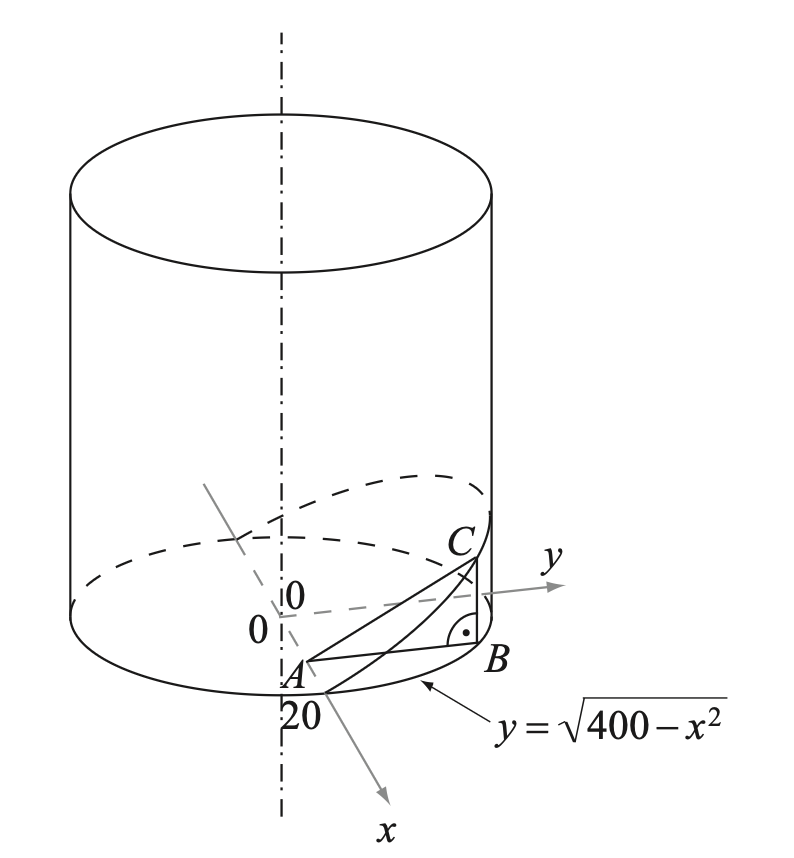
\includegraphics[width = 0.5 \textwidth]{media/keilBaumstamm.png}
	\end{center}

	Berechnen Sie das Volumen des herausgeschnittenen Keils.
\end{ueb}

%% Benötigt so partielle Integraion
% \begin{ueb}
%     {Tarp}{tarp}
%     Betrachten Sie die Abbildung. Eine Gerade in der \(xy\)-Ebene ist durch die Gleichung
%     \[
%         y = g(x) = 1-x
%     \]
%     gegeben. Sie schneidet die \(x\)-Achse in \(A\) und die \(y\)-Achse in \(B\). In der \(xz\)-Ebene ist der Graph der Funktion
%     \[
%         z = f(x) = e^{-x}
%     \]
%     gegeben. Er schneidet die \(z\)-Achse in \(C\).

%     Punkt \(D\) hat die gleiche \(x\)-Koordinate wie \(A\) und liegt auf dem Graphen von \(f\). Die Punkte auf den Graphen von \(g\) und \(f\) werden durch Strecken parallel zur \(yz\)-Ebene verbunden. Dadurch entsteht eine gekrümmte Fläche \(ABCD\).

%     Berechnen Sie das Volumen des Körpers, der durch die Fläche \(ABCD\) und die drei Koordinatenebenen begrenzt wird.
%     \begin{center}
%         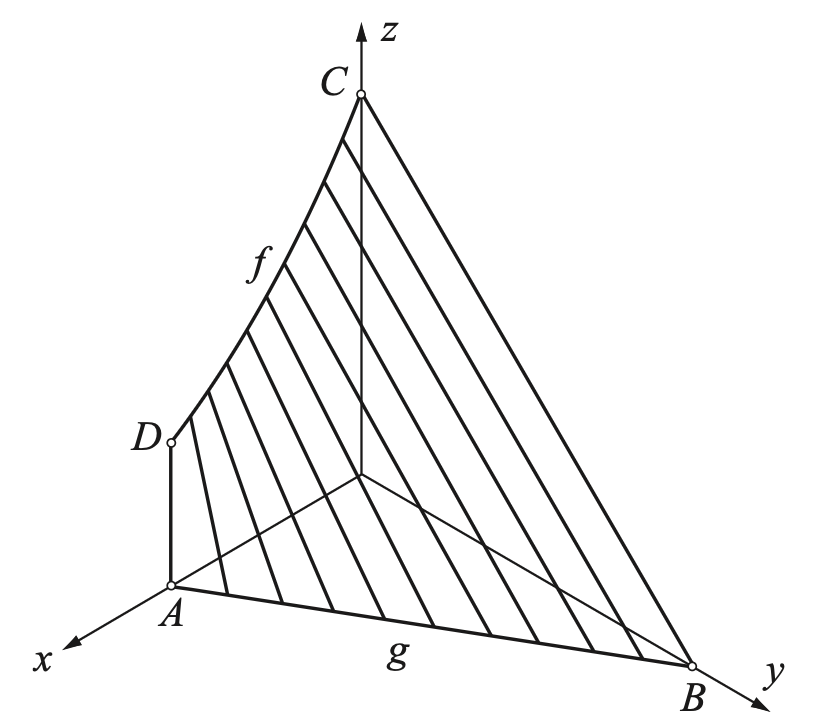
\includegraphics[width = 0.5 \textwidth]{media/Tarp.png}
%     \end{center}

% \end{ueb}

\emph{Lösungen:}
\Cref{uebng:quarterpipe}:\newline

\begin{enumerate}
	\item Die Querschnittsfläche ergibt sich aus der Höhe
	      \[
		      y(x)=\frac{1}{20}x^2
	      \]
	      und der Breite 10 der Quarterpipe. Damit gilt
	      \[
		      A(x)= 10\cdot \frac{1}{20}x^2 = \frac{1}{2}x^2
	      \]

	\item Die maximale Höhe der Pipe ist \(y=20\). Damit kann man den entsprechenden \(x\)-Wert berechnen:
	      \[ 20 = \frac{1}{20}x^2 \Rightarrow x = 20\]
	      Das Volumen der Quarterpipe ist demnach:
	      \[ V = \int_{0}^{20} A(x) dx = \int_0^{20} \frac{1}{2}x^2\,dx
		      =
		      \left[\frac{1}{6}x^3\right]_0^{20}
		      =
		      \frac{4000}{3}\]

	\item Alternativ kann der Körper als Prisma mit der Grundfläche unter der Parabel betrachtet werden:
	      \[
		      V = G\cdot h = \int_0^{20} \frac{1}{20} x^2 dx  \quad \cdot \quad 10 = \frac{400}{3} \cdot 10 =  \frac{4000}{3}
	      \]
	      Beide Berechnungen liefern dasselbe Resultat.
\end{enumerate}

\emph{Lösungen:}\Cref{uebng:keil}

Für einen Querschnitt im Abstand \(x\) vom Mittelpunkt gilt \(\overline{AB} = \sqrt{400-x^2}\) und \(\overline{BC} = \overline{AB} \cdot \tan(30^\circ)\). Damit folgt:
\[
	A(x)=\frac{1}{2}\sqrt{400-x^2} \cdot \sqrt{400-x^2}\tan(30^\circ) = \frac{\sqrt{3}}{6}\left(400-x^2\right)
\]
Damit
\[
	V=\int_{-20}^{20} A(x)\,dx
	=\frac{2}{3}r^3\tan(30^\circ)
	=\frac{16000}{3\sqrt{3}}\,\si{\centi\metre\cubed}
	\approx \SI{3079}{\centi\metre\cubed}
\]






% \clearpage
% \textbf{Mittelwert einer Funktion}
% \begin{LA}
%     {Der Mittelwert einer Funktion}{}
%     In Breitengraden wie jenem von Zürich kann die Tageslänge von Sonnenaufgang bis Sonnenuntergang grob durch die Funktion mit der Gleichung 
%     $$ T(x) = 4 \sin\left(\frac{2\pi}{365} (x-80)\right) +12 $$
%     angenähert werden, wobei $x$ die Nummer des Tages im Jahr und $T$ die Tageslänge in Stunden ist.
%     \begin{enumerate}
%         \item Zeichnen Sie den Graphen der Funktion mit Geogebra im Bereich $x\in[0, 365]$. An welchem Datum sind Tag und Nacht gleich lang? Wann ist der längste/kürzeste Tag?
%         \item Welches ist die mittlere Tageslänge über ein Jahr betrachtet?
%         \item Allgemein versteht man unter dem \emph{Mittelwert} einer positiven stetigen Funktion $y=f(x)$ im Intervall $x\in[a,b]$, jenen Wert $y_M$, bei dem der Flächeninhalt des Rechtecks mit der Höhe $y_M$ über dem Intervall $[a,b]$ gleich gross ist wie der Flächeninhalt des Gebietes zwischen dem Graphen von $f$ und der $x$-Achse im Intervall $[a,b]$.

%         Stellen Sie eine Gleichung für $y_M$ auf und berechnen Sie damit die mittlere Tageslänge.
%     \end{enumerate}
% \end{LA}
% \clearpage
% \begin{definition}
%     {Mittelwert einer Funktion}{}
% \begin{center}
%     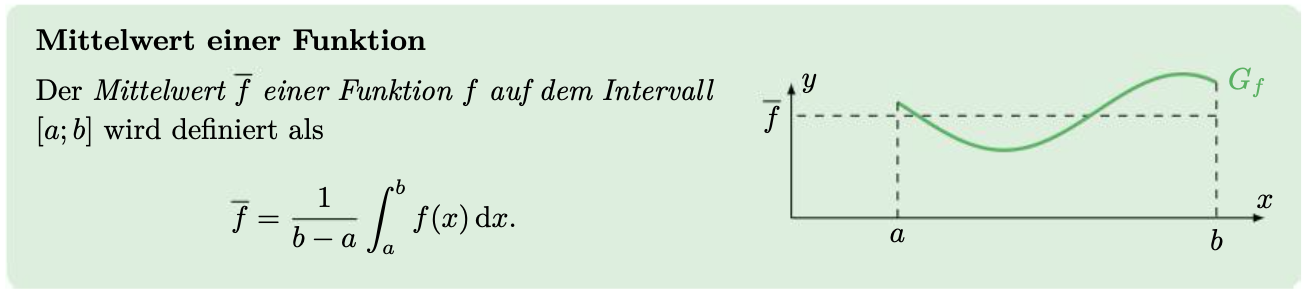
\includegraphics[width = \textwidth]{media/defMittelwert.png}
% \end{center}
% \end{definition}

% \begin{bsp}
%     {Mittelwert einer Funktion}{}
%     Der Mittelwert der Funktion $f(x)=x^2$ im Intervall $[0,1]$ ist:
%     $$ \bar{f} = \frac{1}{1-0}\int_0^1 x^2 \, dx = \frac{1}{3}$$
%     \begin{center}
%         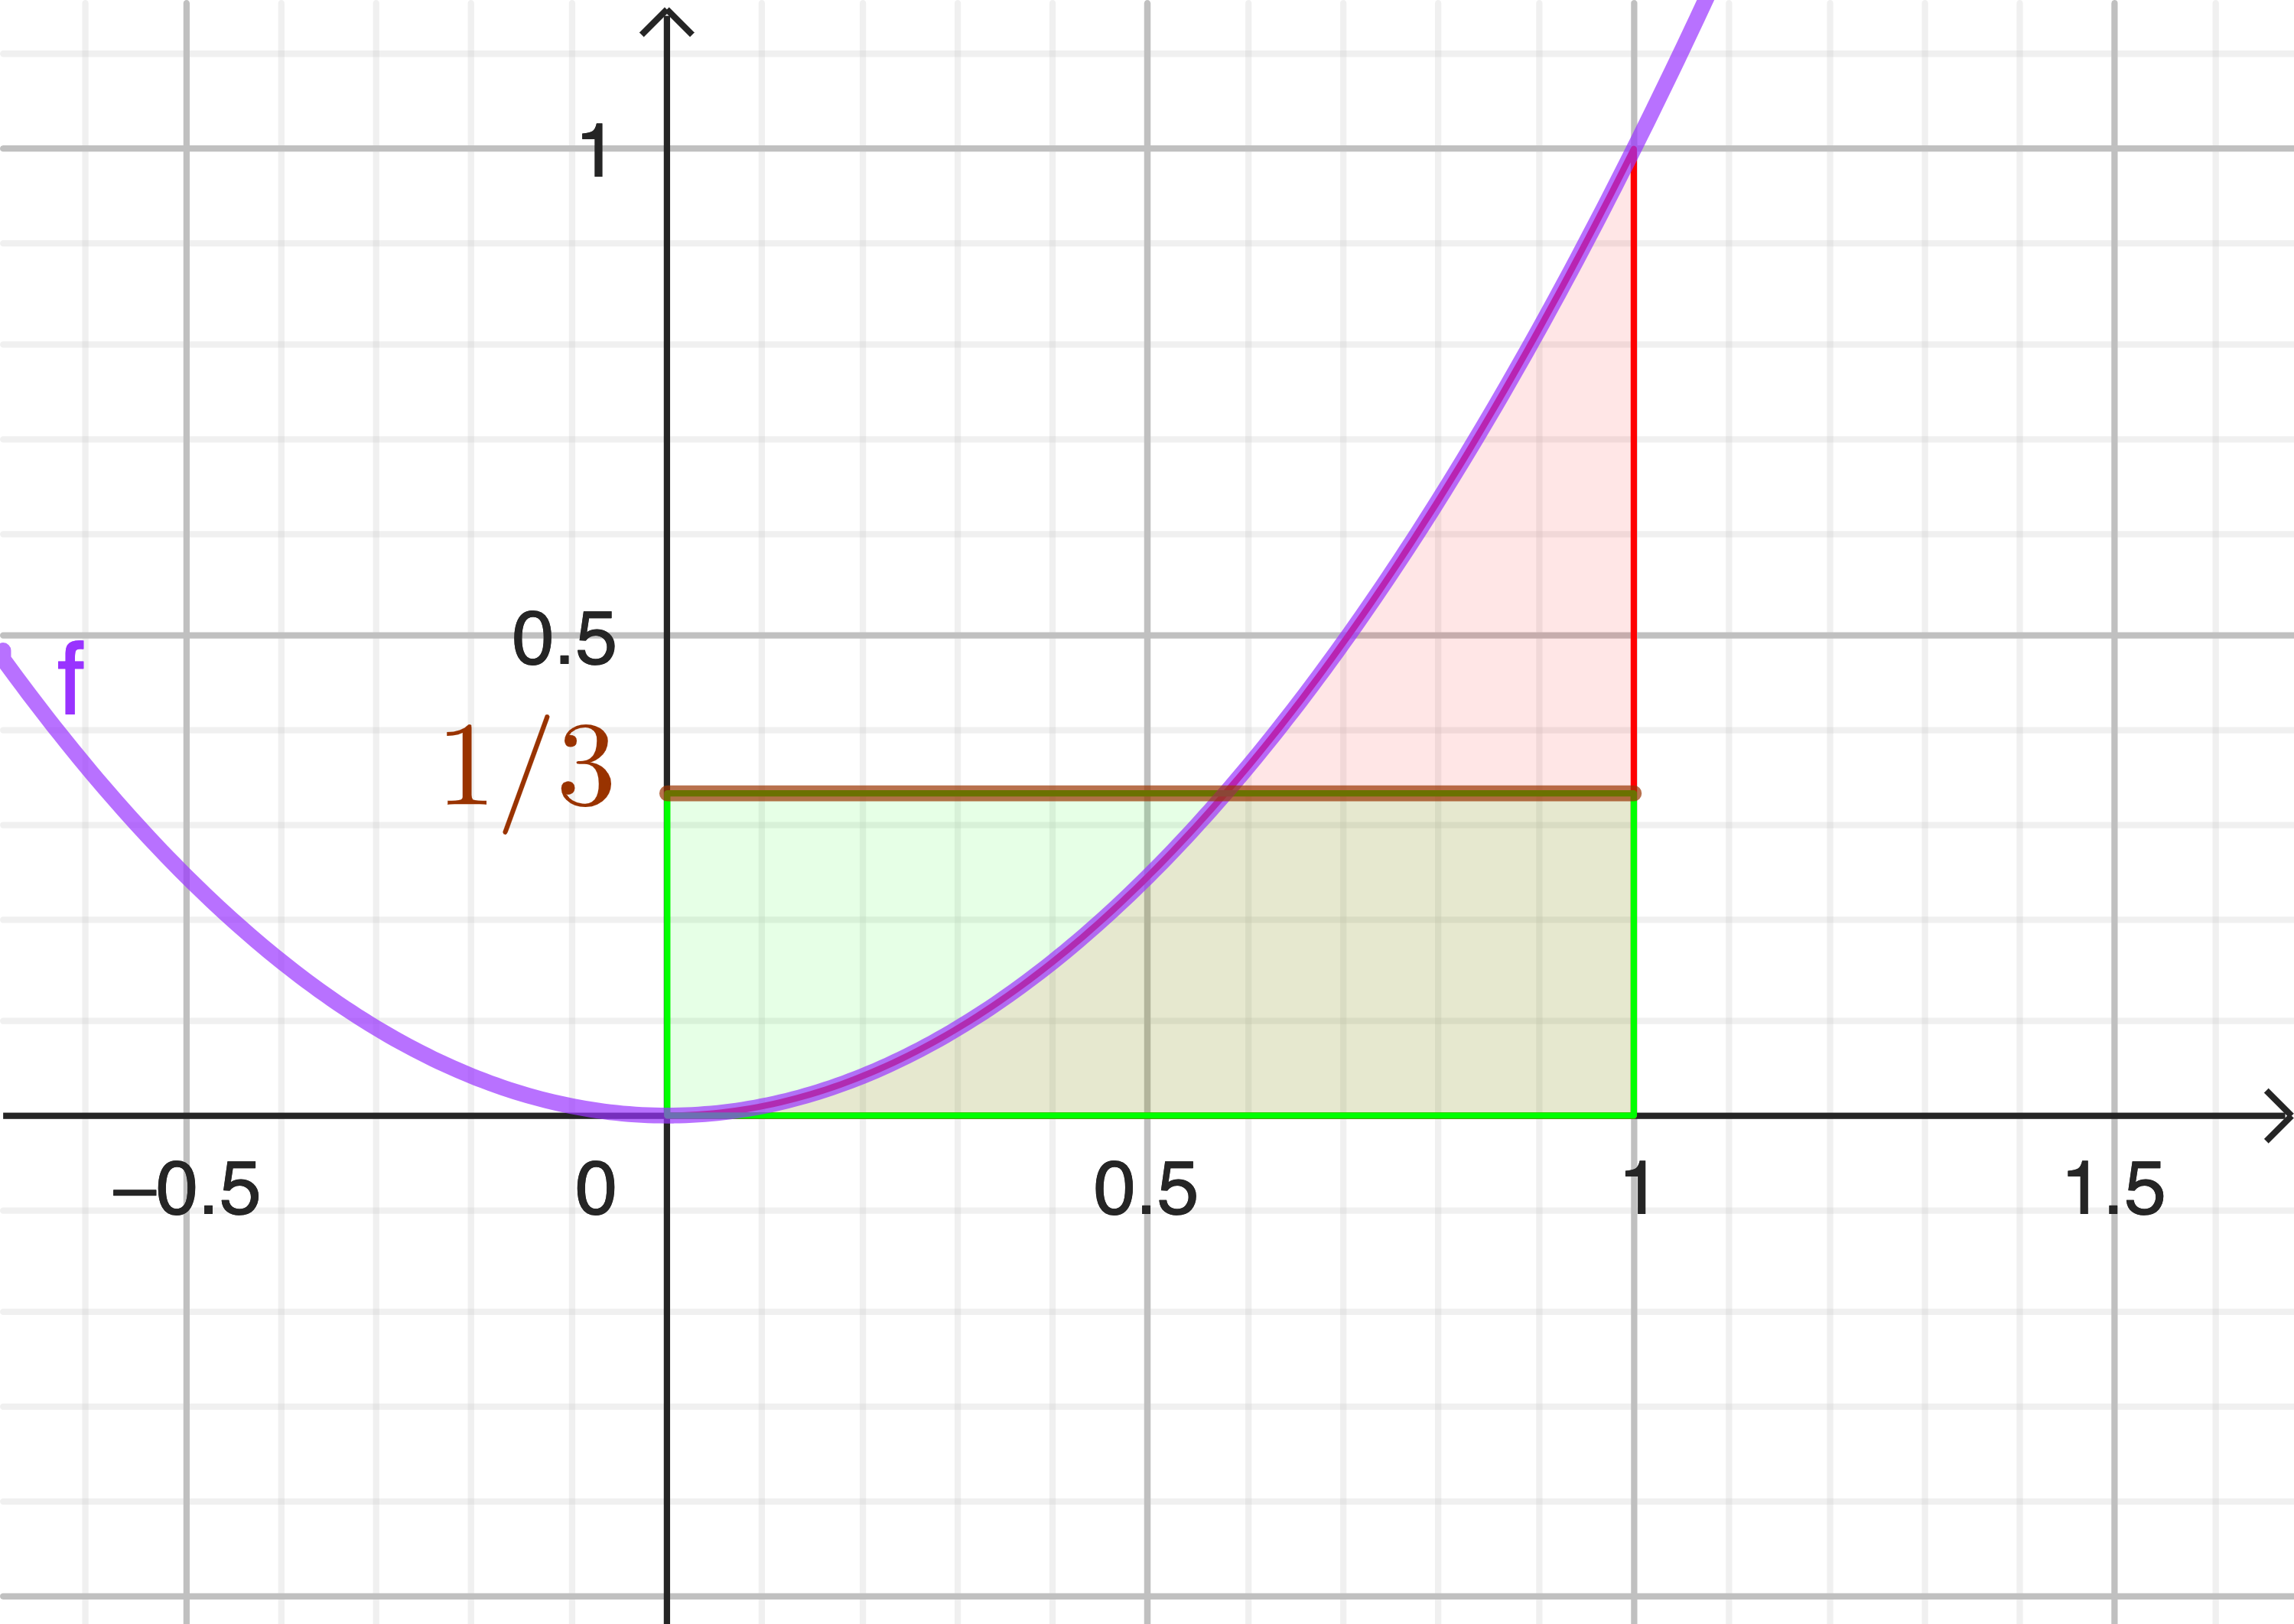
\includegraphics[width = 0.5 \textwidth]{media/bspMittelwert.png}
%     \end{center}
% \end{bsp}




\clearpage
\subsection{Uneigentliche Integrale}
\begin{bsp}
	{Zwei typische Fragestellungen}{}
	Der Graph der Funktion $f(x) = \frac{1}{x}, \, x \in [1, \infty[$ erstreckt sich ins Unendliche. Im Folgenden untersuchen wir einerseits den Flächeninhalt $A$ des Gebietes $G$ zwischen dem Graphen von $f$ und der $x$-Achse und andererseits den Rauminhalt $V$ des Körpers, der durch Rotation von $G$ um die $x$-Achse entsteht.
	\begin{enumerate}
		\item Bestimme $A(t) = \int_1^t f(x) dx$ und $V(t) = \pi \int_1^t (f(x))^2 dx$ für $t\in [1, \infty[$
		\item Bestimme $\lim_{t\to\infty} A(t)$ und $\lim_{t\to\infty} V(t)$, falls die Grenzwerte existieren.
	\end{enumerate}
\end{bsp}
\clearpage
\begin{definition}
	{Uneigentliche Integrale}{}
	\begin{center}
		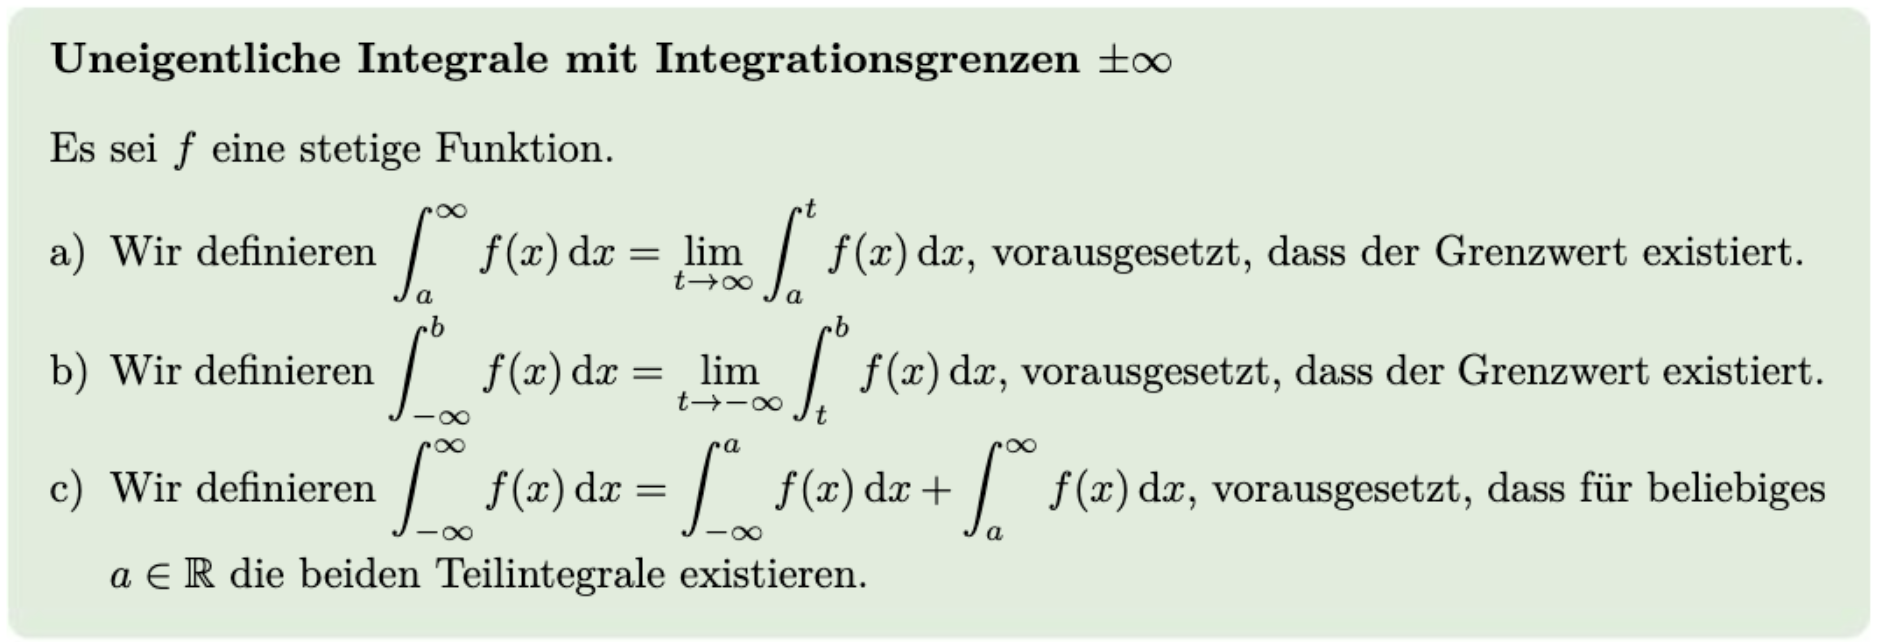
\includegraphics[width = \textwidth]{media/defUneigentlicheIntegrale.png}
	\end{center}
\end{definition}
\begin{bsp}
	{Ein uneigentliches Integral}{}
	\begin{align*}
		\int_{4}^{\infty} \frac{4-x}{x^3} \,dx & = \lim_{{t \to \infty}} \int_{4}^{t} \frac{4-x}{x^3} \,dx                                      \\
		                                       & = \lim_{{t \to \infty}} \int_{4}^{t} \left( \frac{4}{x^3} - \frac{1}{x^2} \right) \,dx         \\
		                                       & = \lim_{{t \to \infty}} \int_{4}^{t} \left( 4\cdot x^{-3} - x^{-2} \right) \,dx                \\
		                                       & = \lim_{{t \to \infty}} \left[ 4\cdot \left(-\frac{1}{2}\right)x^{-2} + x^{-1} \right]_{4}^{t} \\
		                                       & = \lim_{{t \to \infty}} \left( -2t^{-2} + t^{-1} - (-2 \cdot 4^{-2} + 4^{-1}) \right)          \\
		                                       & = 0 + 0 - \left( -\frac{1}{8} + \frac{1}{4} \right)                                            \\
		                                       & = -\frac{1}{8}
	\end{align*}
	\begin{center}
		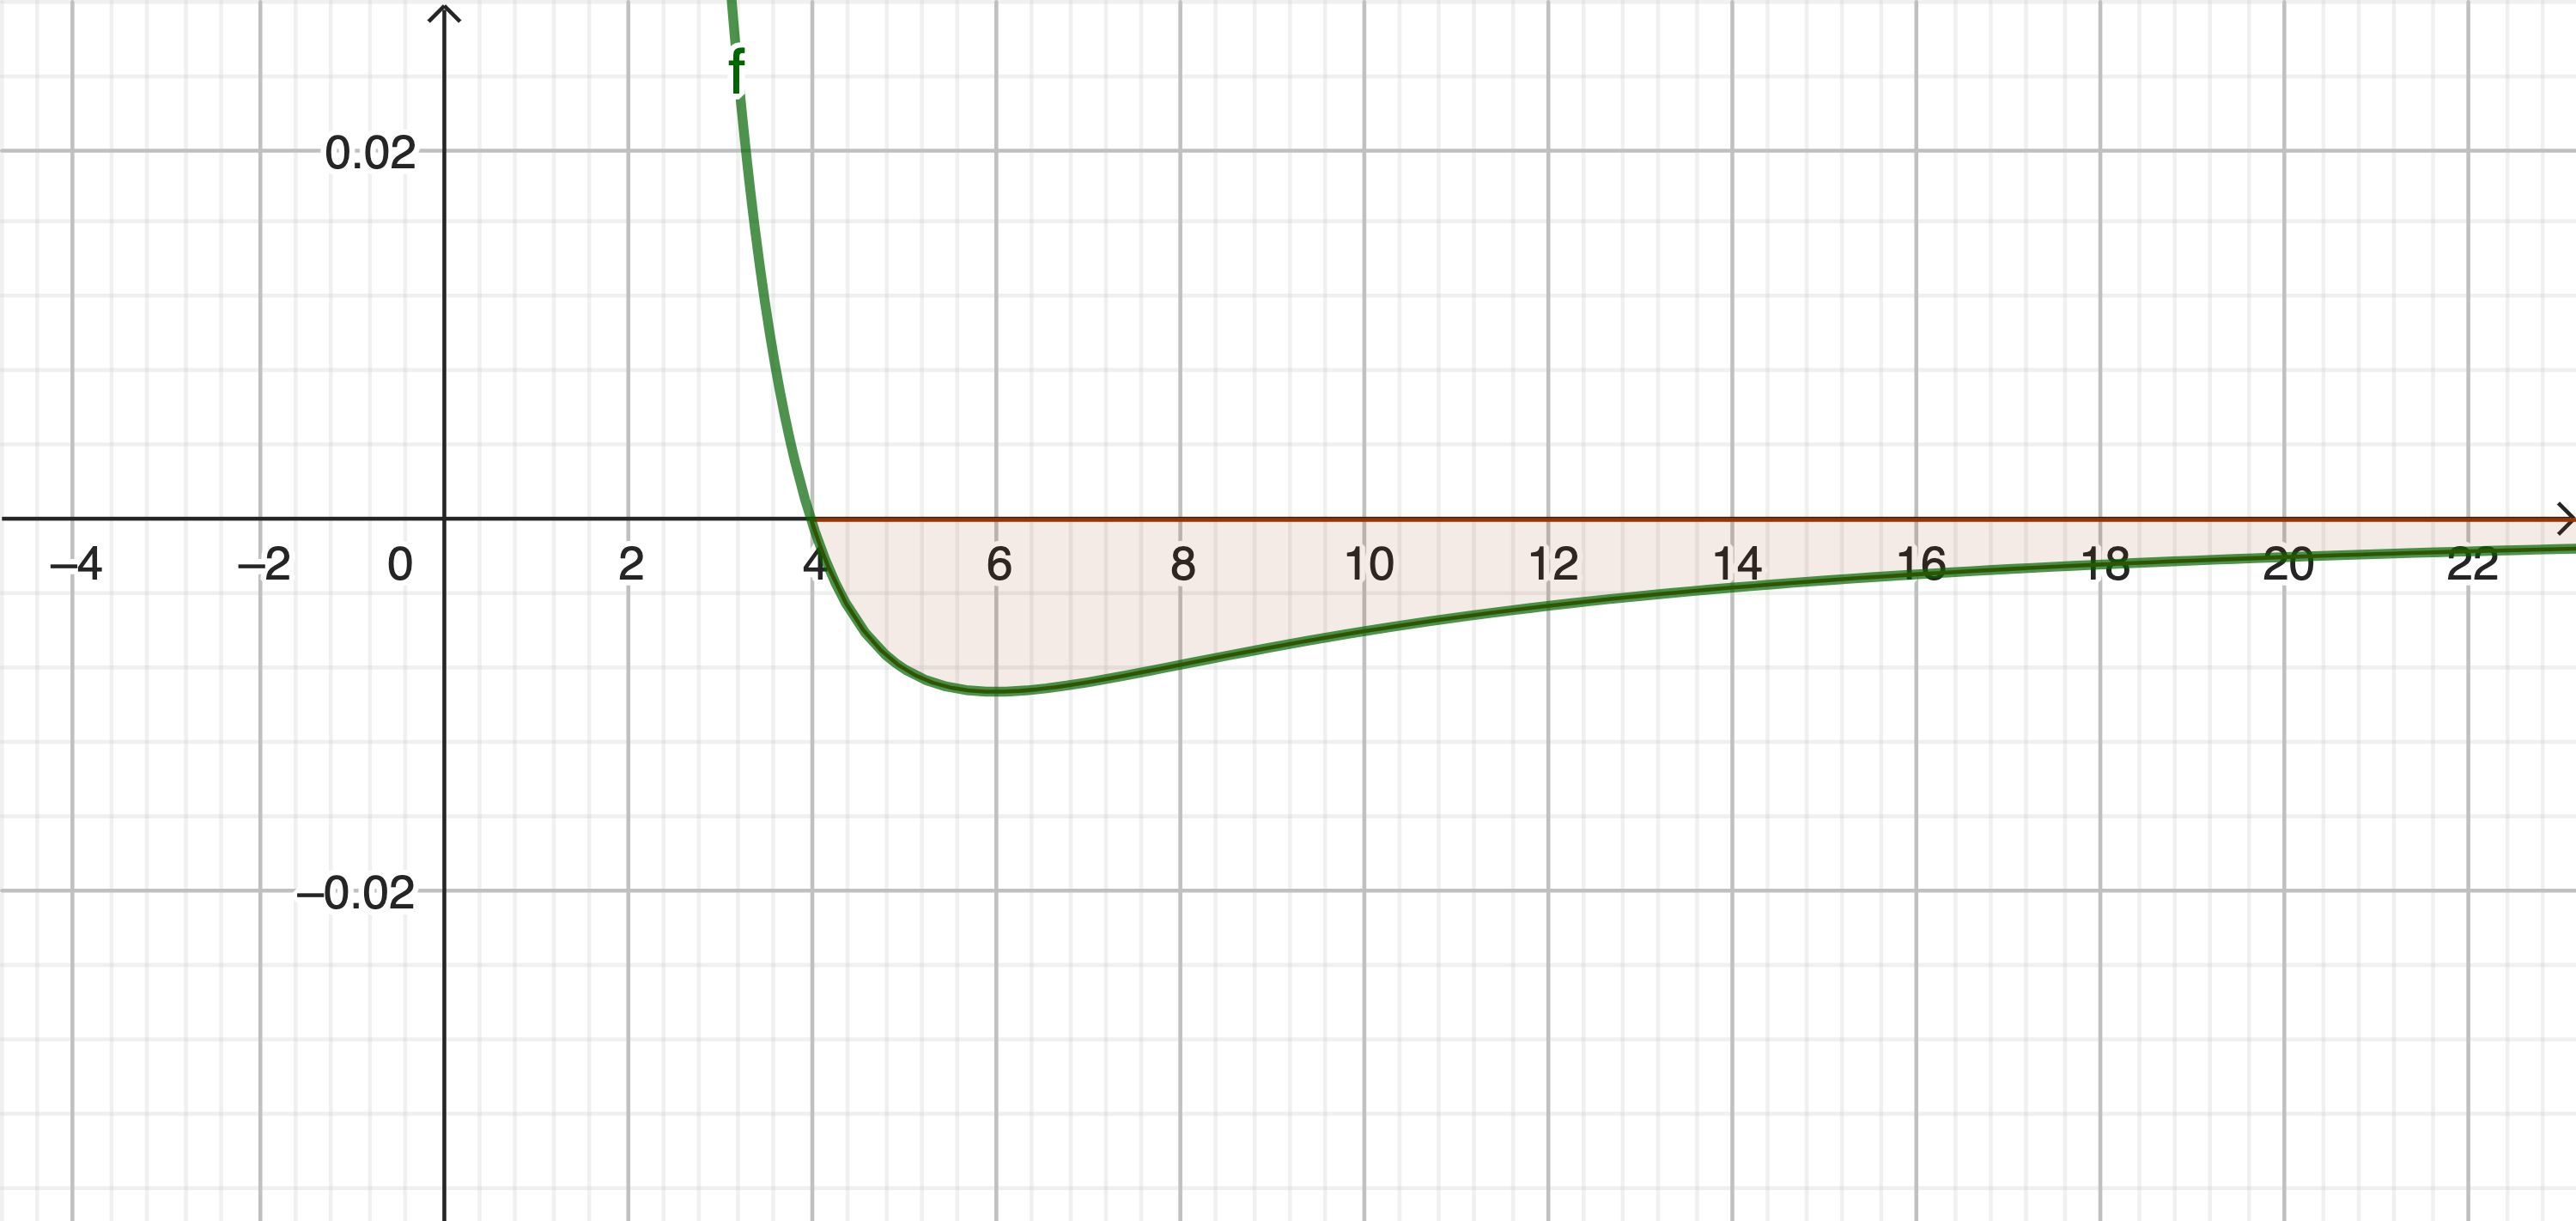
\includegraphics[width = 0.5 \textwidth]{media/bspUneigentlich.png}
	\end{center}
\end{bsp}
\clearpage
\begin{bsp}
	{Ein uneigentliches Integral mit linearer Substitution}{}
	$$\int_{3}^{\infty} \frac{1}{(2x+1)^2} dx = ?$$
	Die Stammfunktion lässt sich mit linearer Substitution finden: $$\int \frac{1}{(2x+1)^2} dx= \int (2x+1) ^{-2} dx= -(2x+1)^{-1}\cdot \frac{1}{2} + C$$
	Damit folgt:
	\begin{align*}
		\int_{3}^{\infty} \frac{1}{(2x+1)^2} dx & = \lim_{t \to \infty}  \int_{3}^{t} (2x+1) ^{-2} dx                                         \\
		                                        & = \lim_{t \to \infty} \left[-(2x+1)^{-1}\cdot \frac{1}{2}\right]_3^t                        \\
		                                        & = \lim_{t \to \infty} \left(-\frac{1}{(2t+1)\cdot 2} + \frac{1}{(2\cdot 3+1)\cdot 2}\right) \\
		                                        & = \frac{1}{14}
	\end{align*}
	\begin{center}
		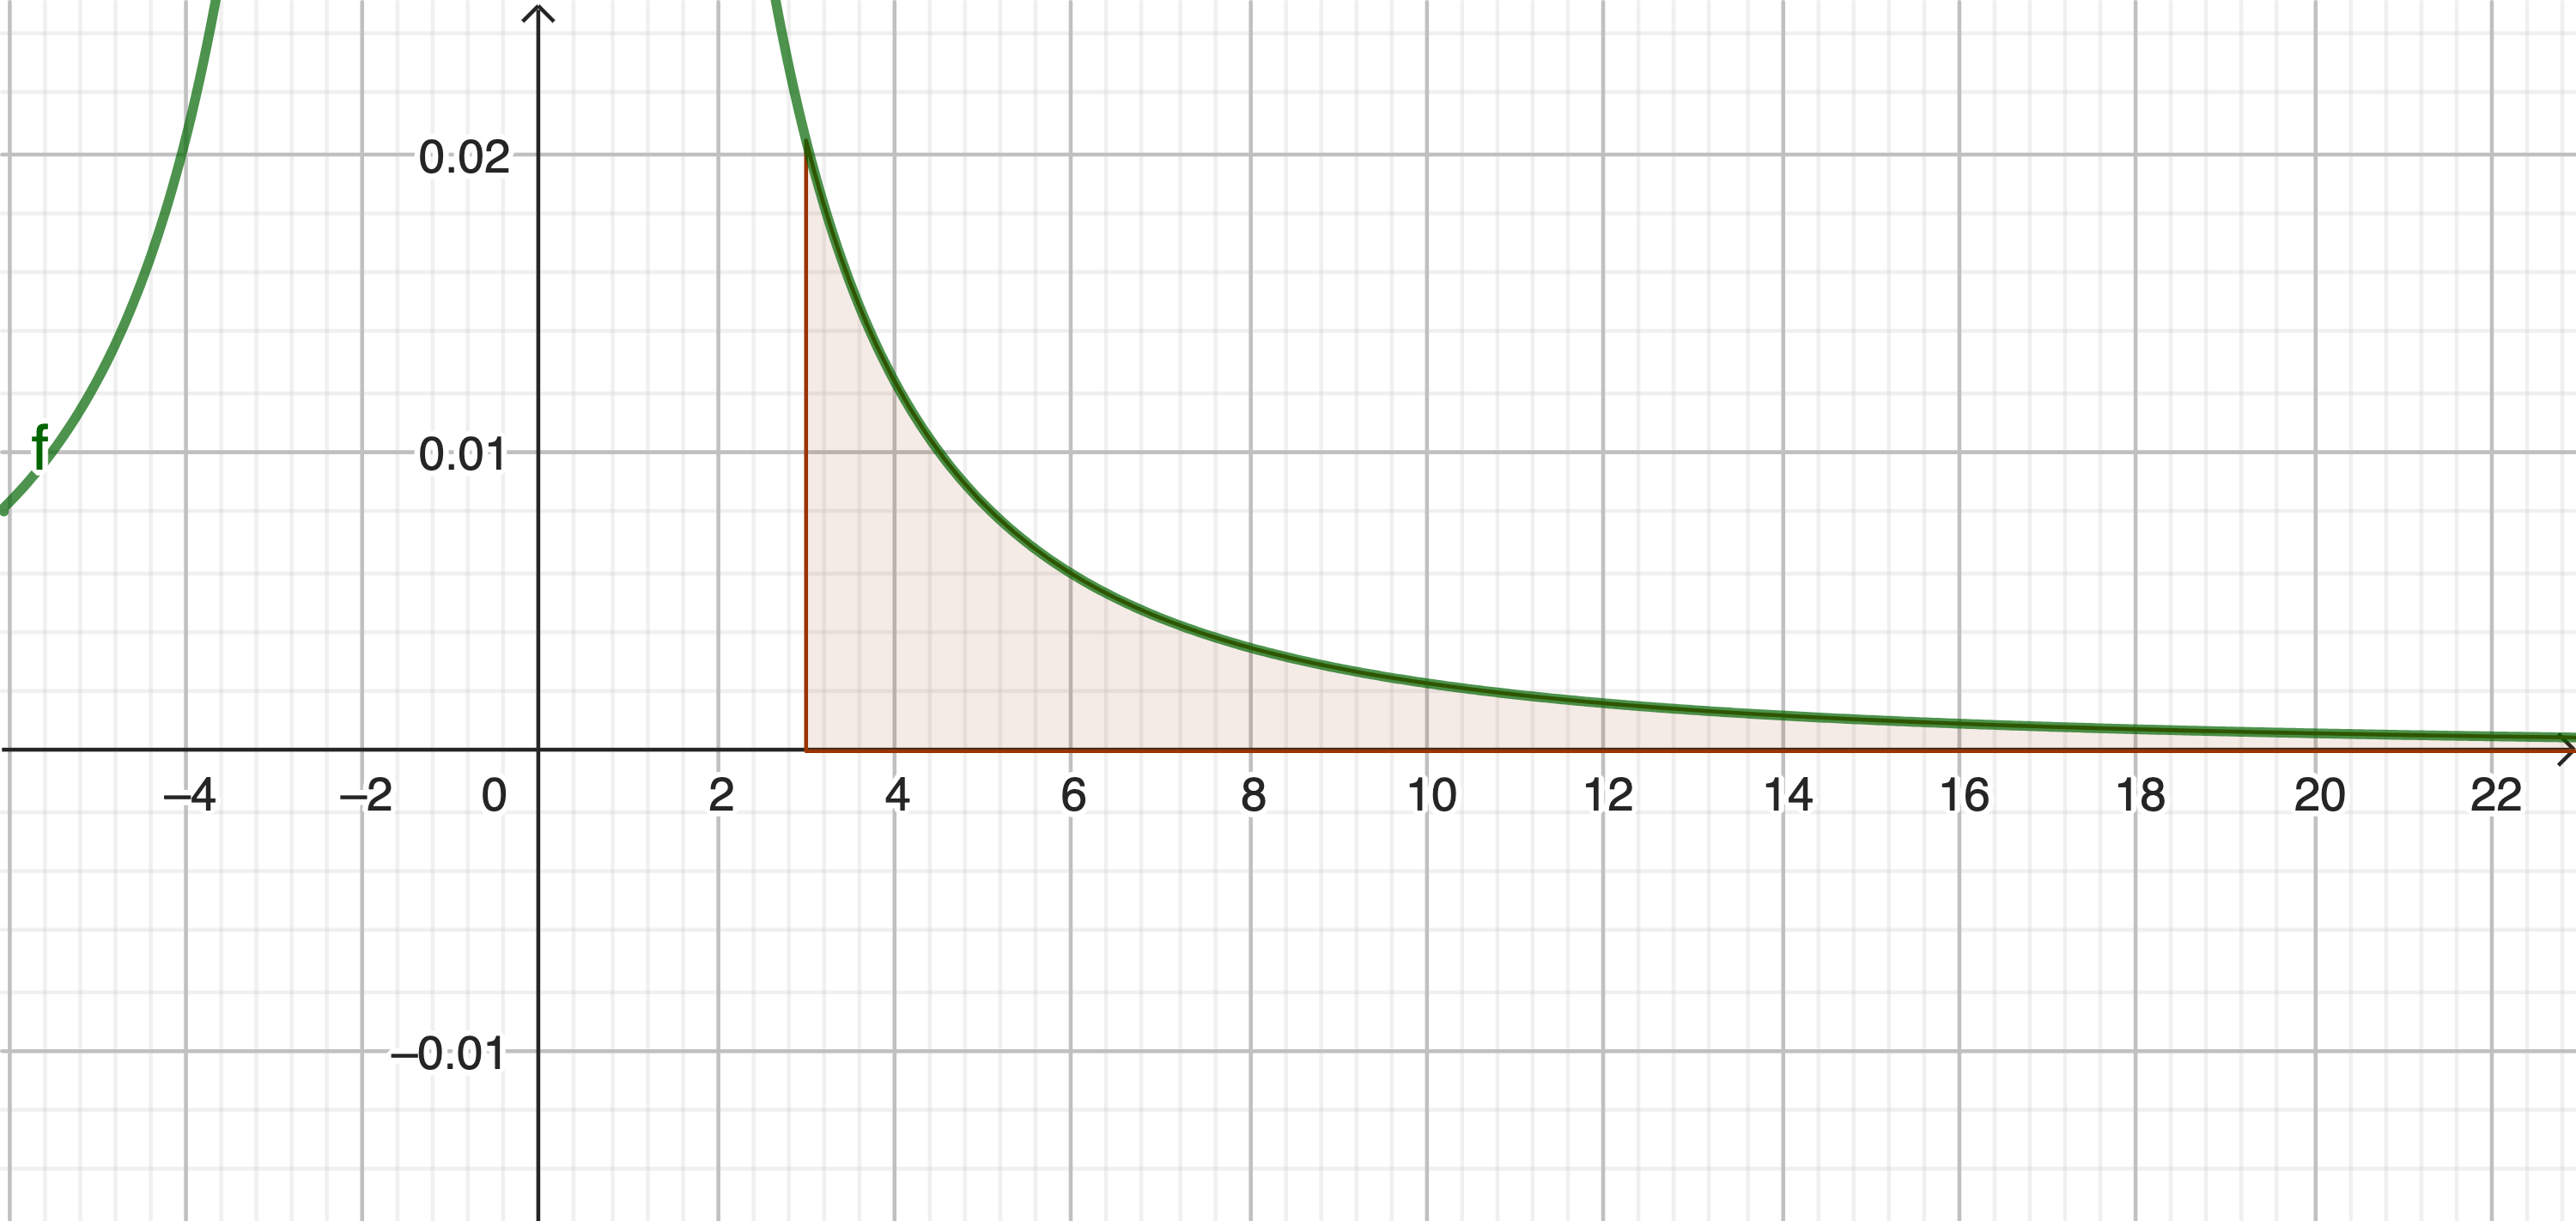
\includegraphics[width = 0.5 \textwidth]{media/bspUneigentlich2.png}
	\end{center}
\end{bsp}

\clearpage
\subsection{Breitgefächerte Anwendungen}
\subsubsection*{Aus der Geometrie}
\begin{bsp}
    {Kippende Schale - Aufgabe 155 im Buch}{}
    Eine auf dem Gartentisch liegende Halbkugelschale aus Glas ist randvoll mit Wasser gefüllt. Um welchen Winkel muss die Schale geneigt werden, damit exakt die Hälfte des Wassers ausfliesst?
    \begin{center}
        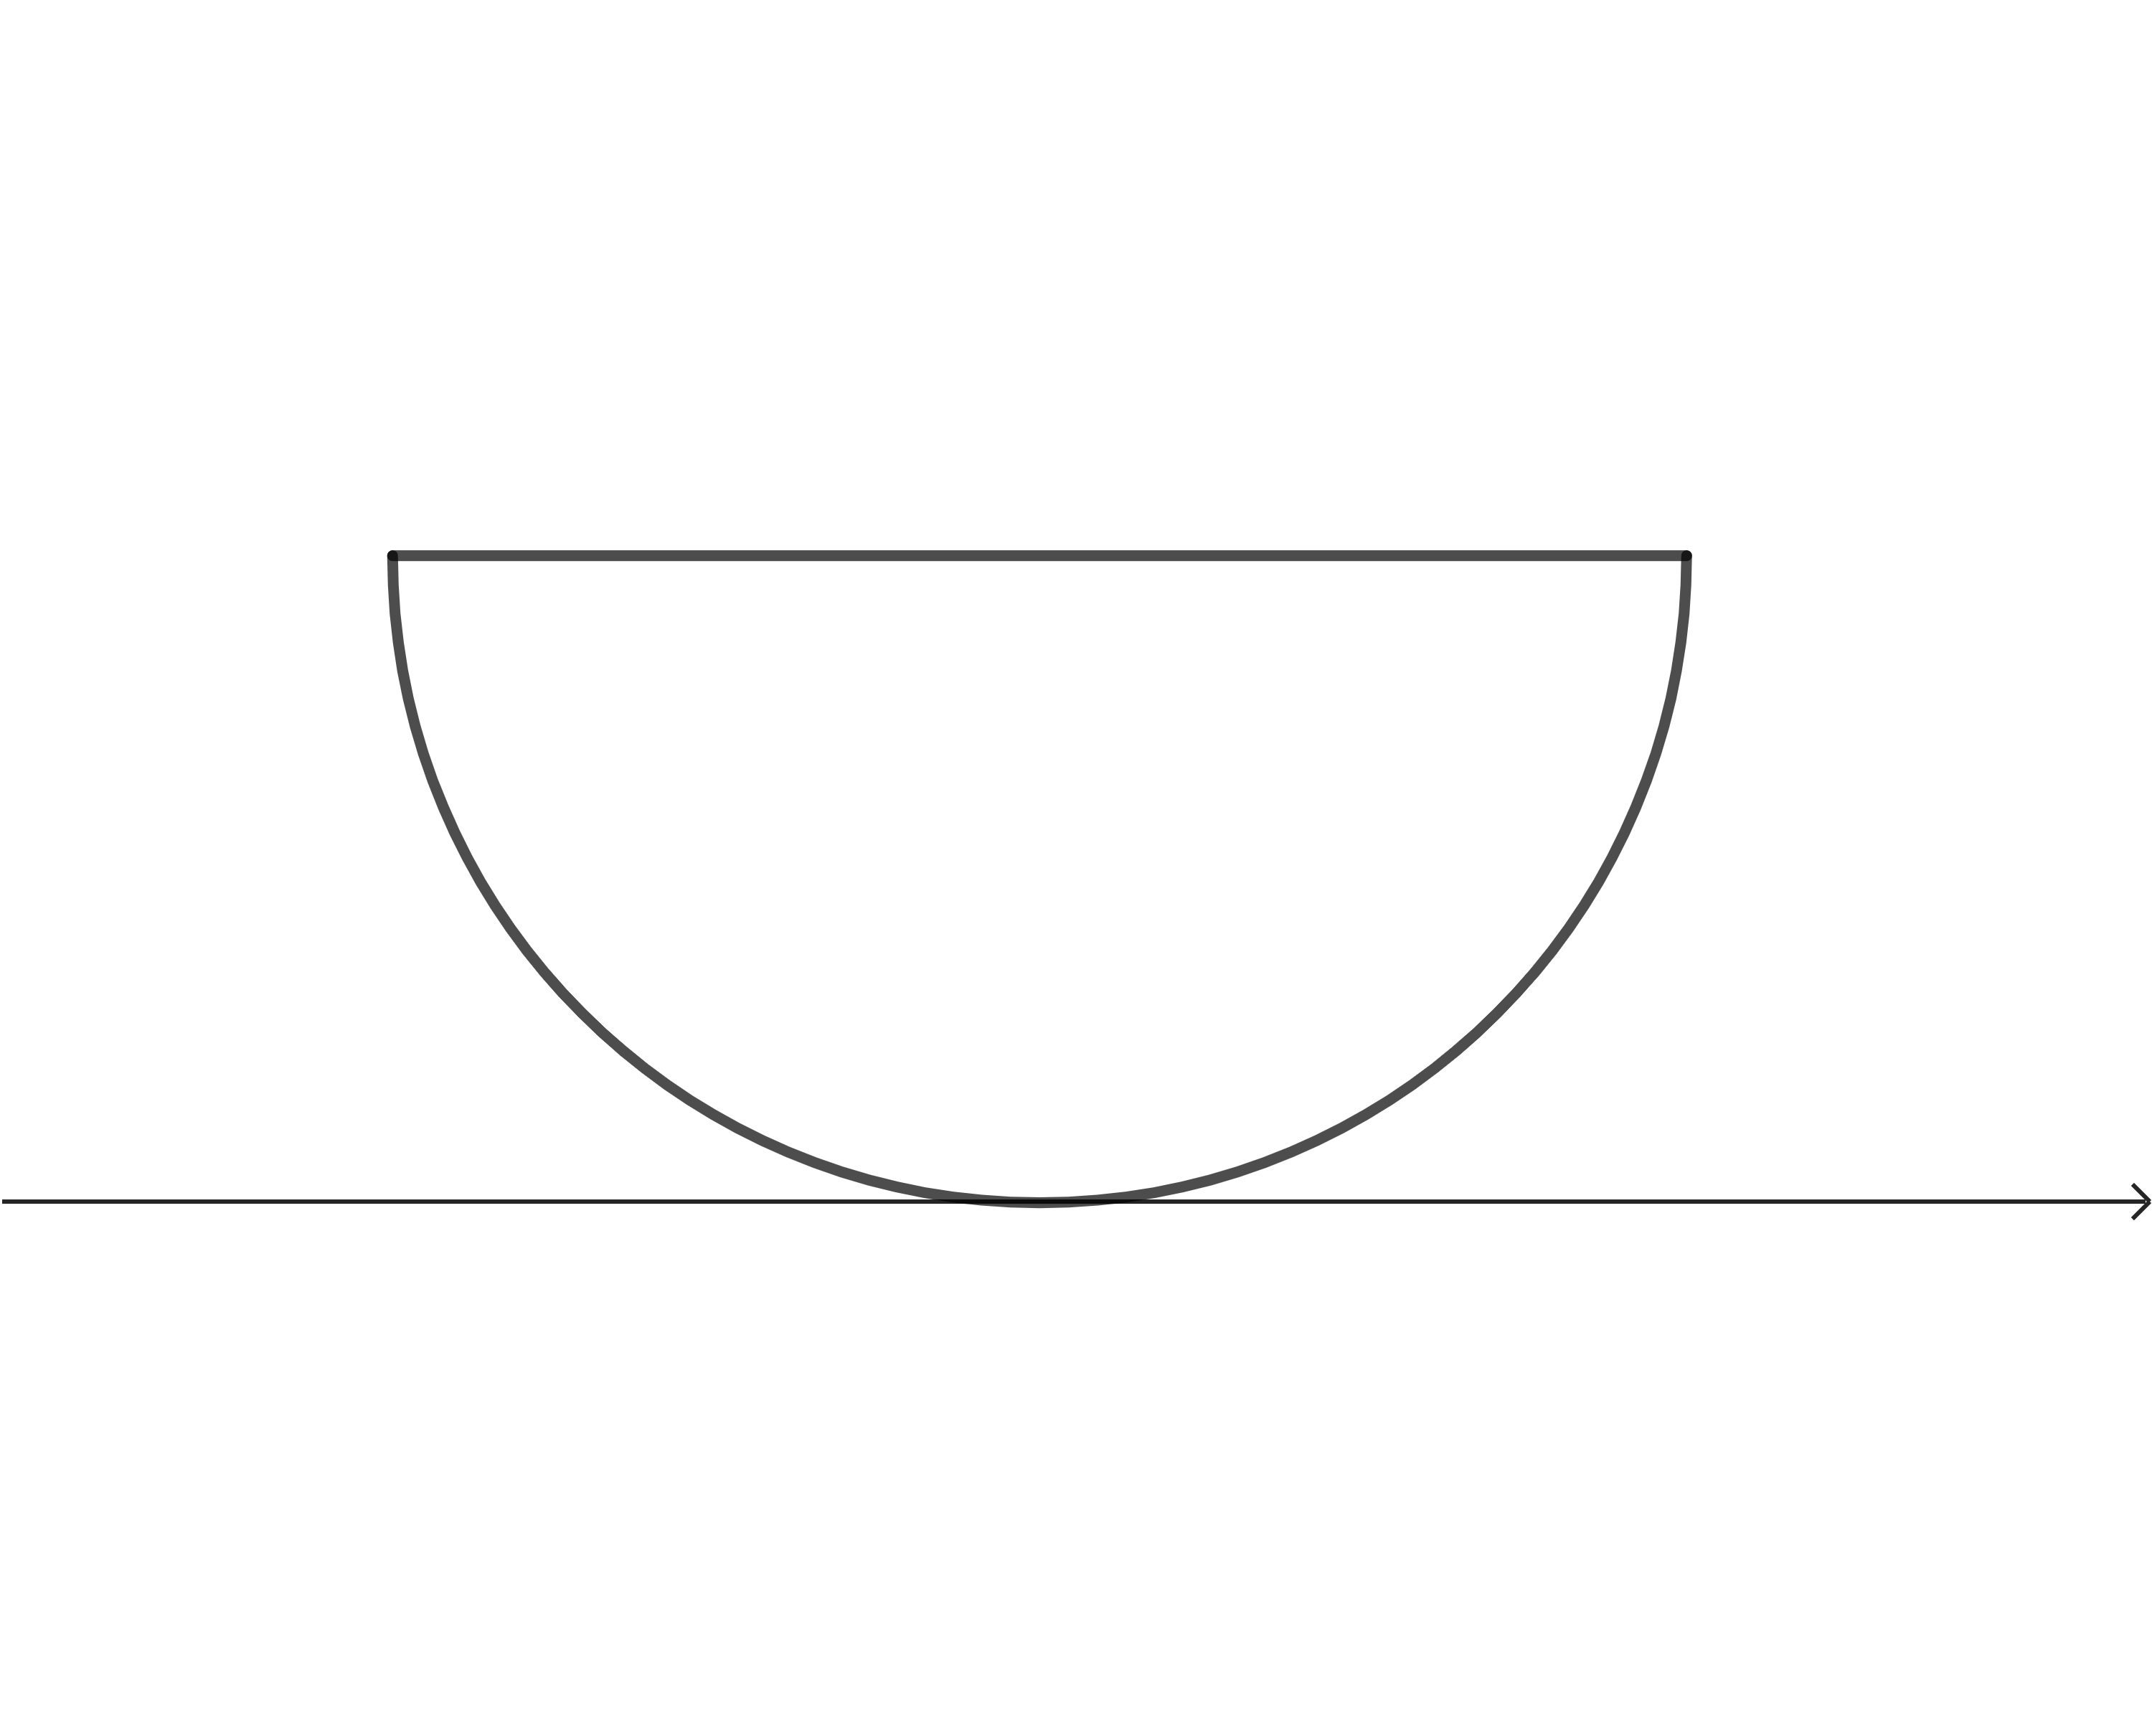
\includegraphics[width = 0.4\textwidth]{media/DMK155-1.png}\hfill
        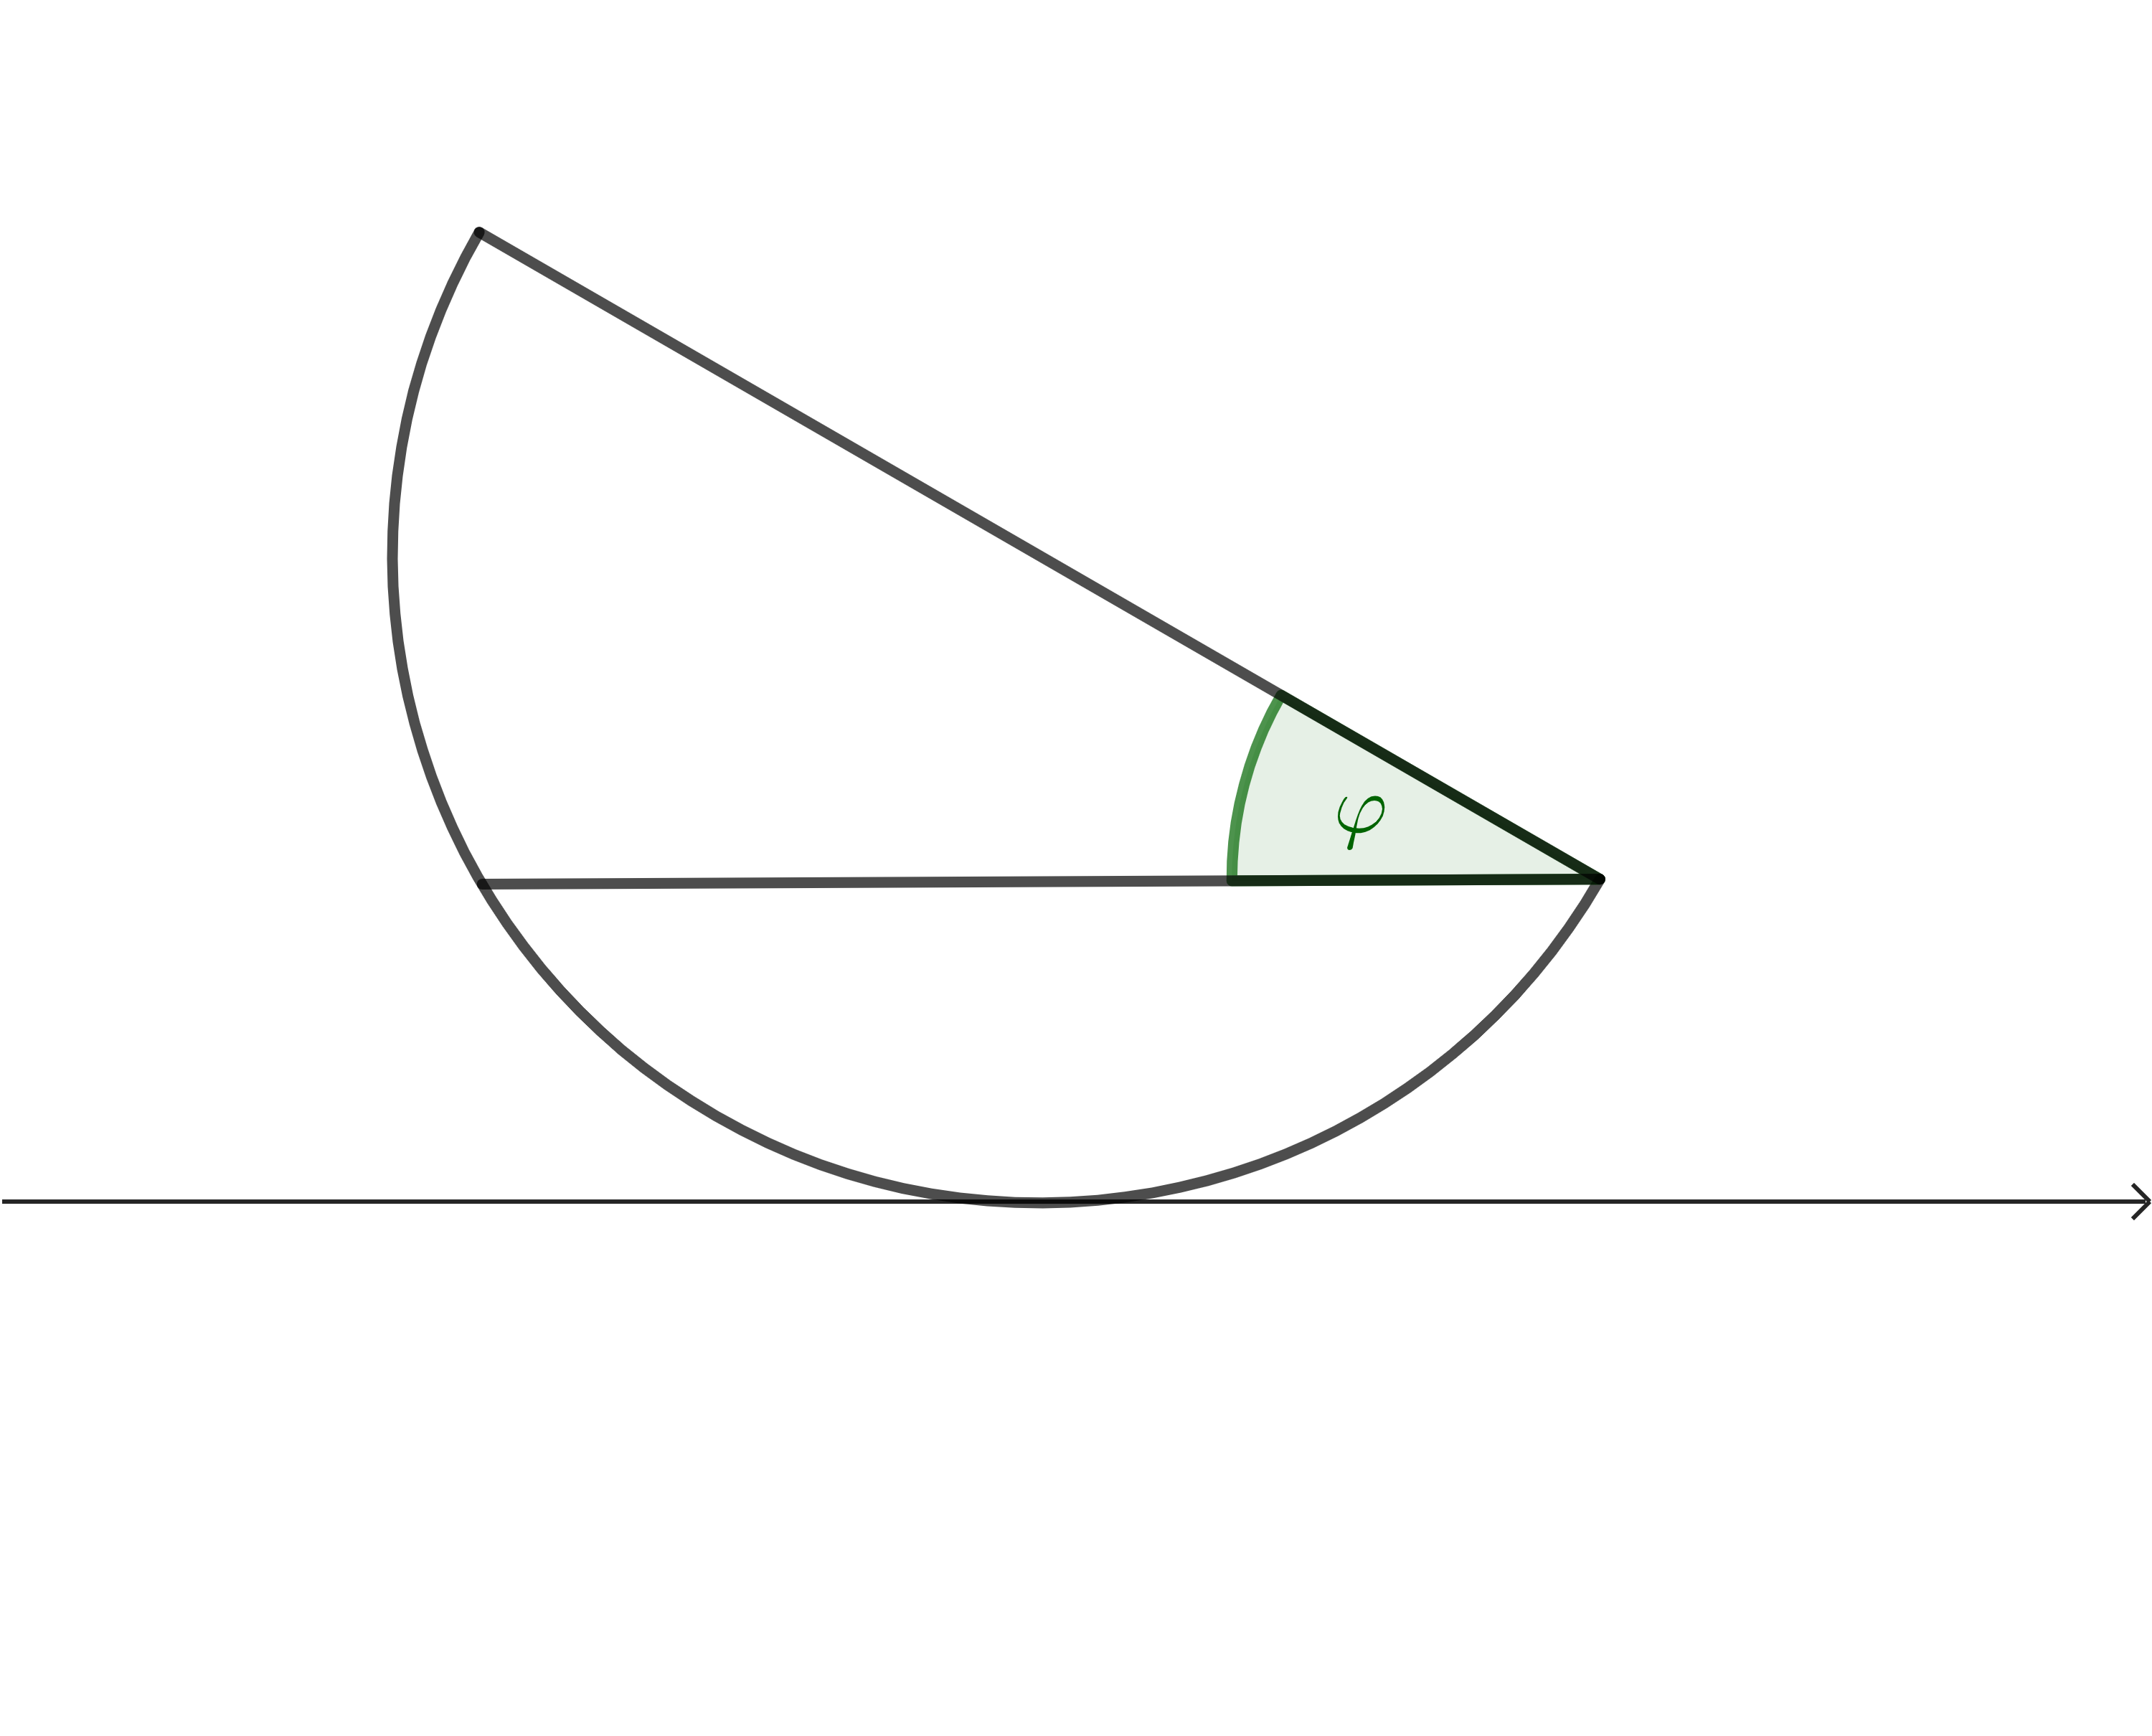
\includegraphics[width = 0.4\textwidth]{media/DMK155-2.png}
    \end{center}
\end{bsp}
\clearpage
\subsubsection*{Aus der Physik}

Wenn ein Körper sich mit konstanter Geschwindigkeit bewegt, lässt sich der zurückgelegte Weg als das Produkt aus Zeit und Geschwindigkeit berechnen:
$$ \Delta  s = v\cdot \Delta t$$
Grafisch kann das Produkt aus Zeit und Geschwindigkeit als Flächeninhalt interpretiert werden:
\begin{center}
    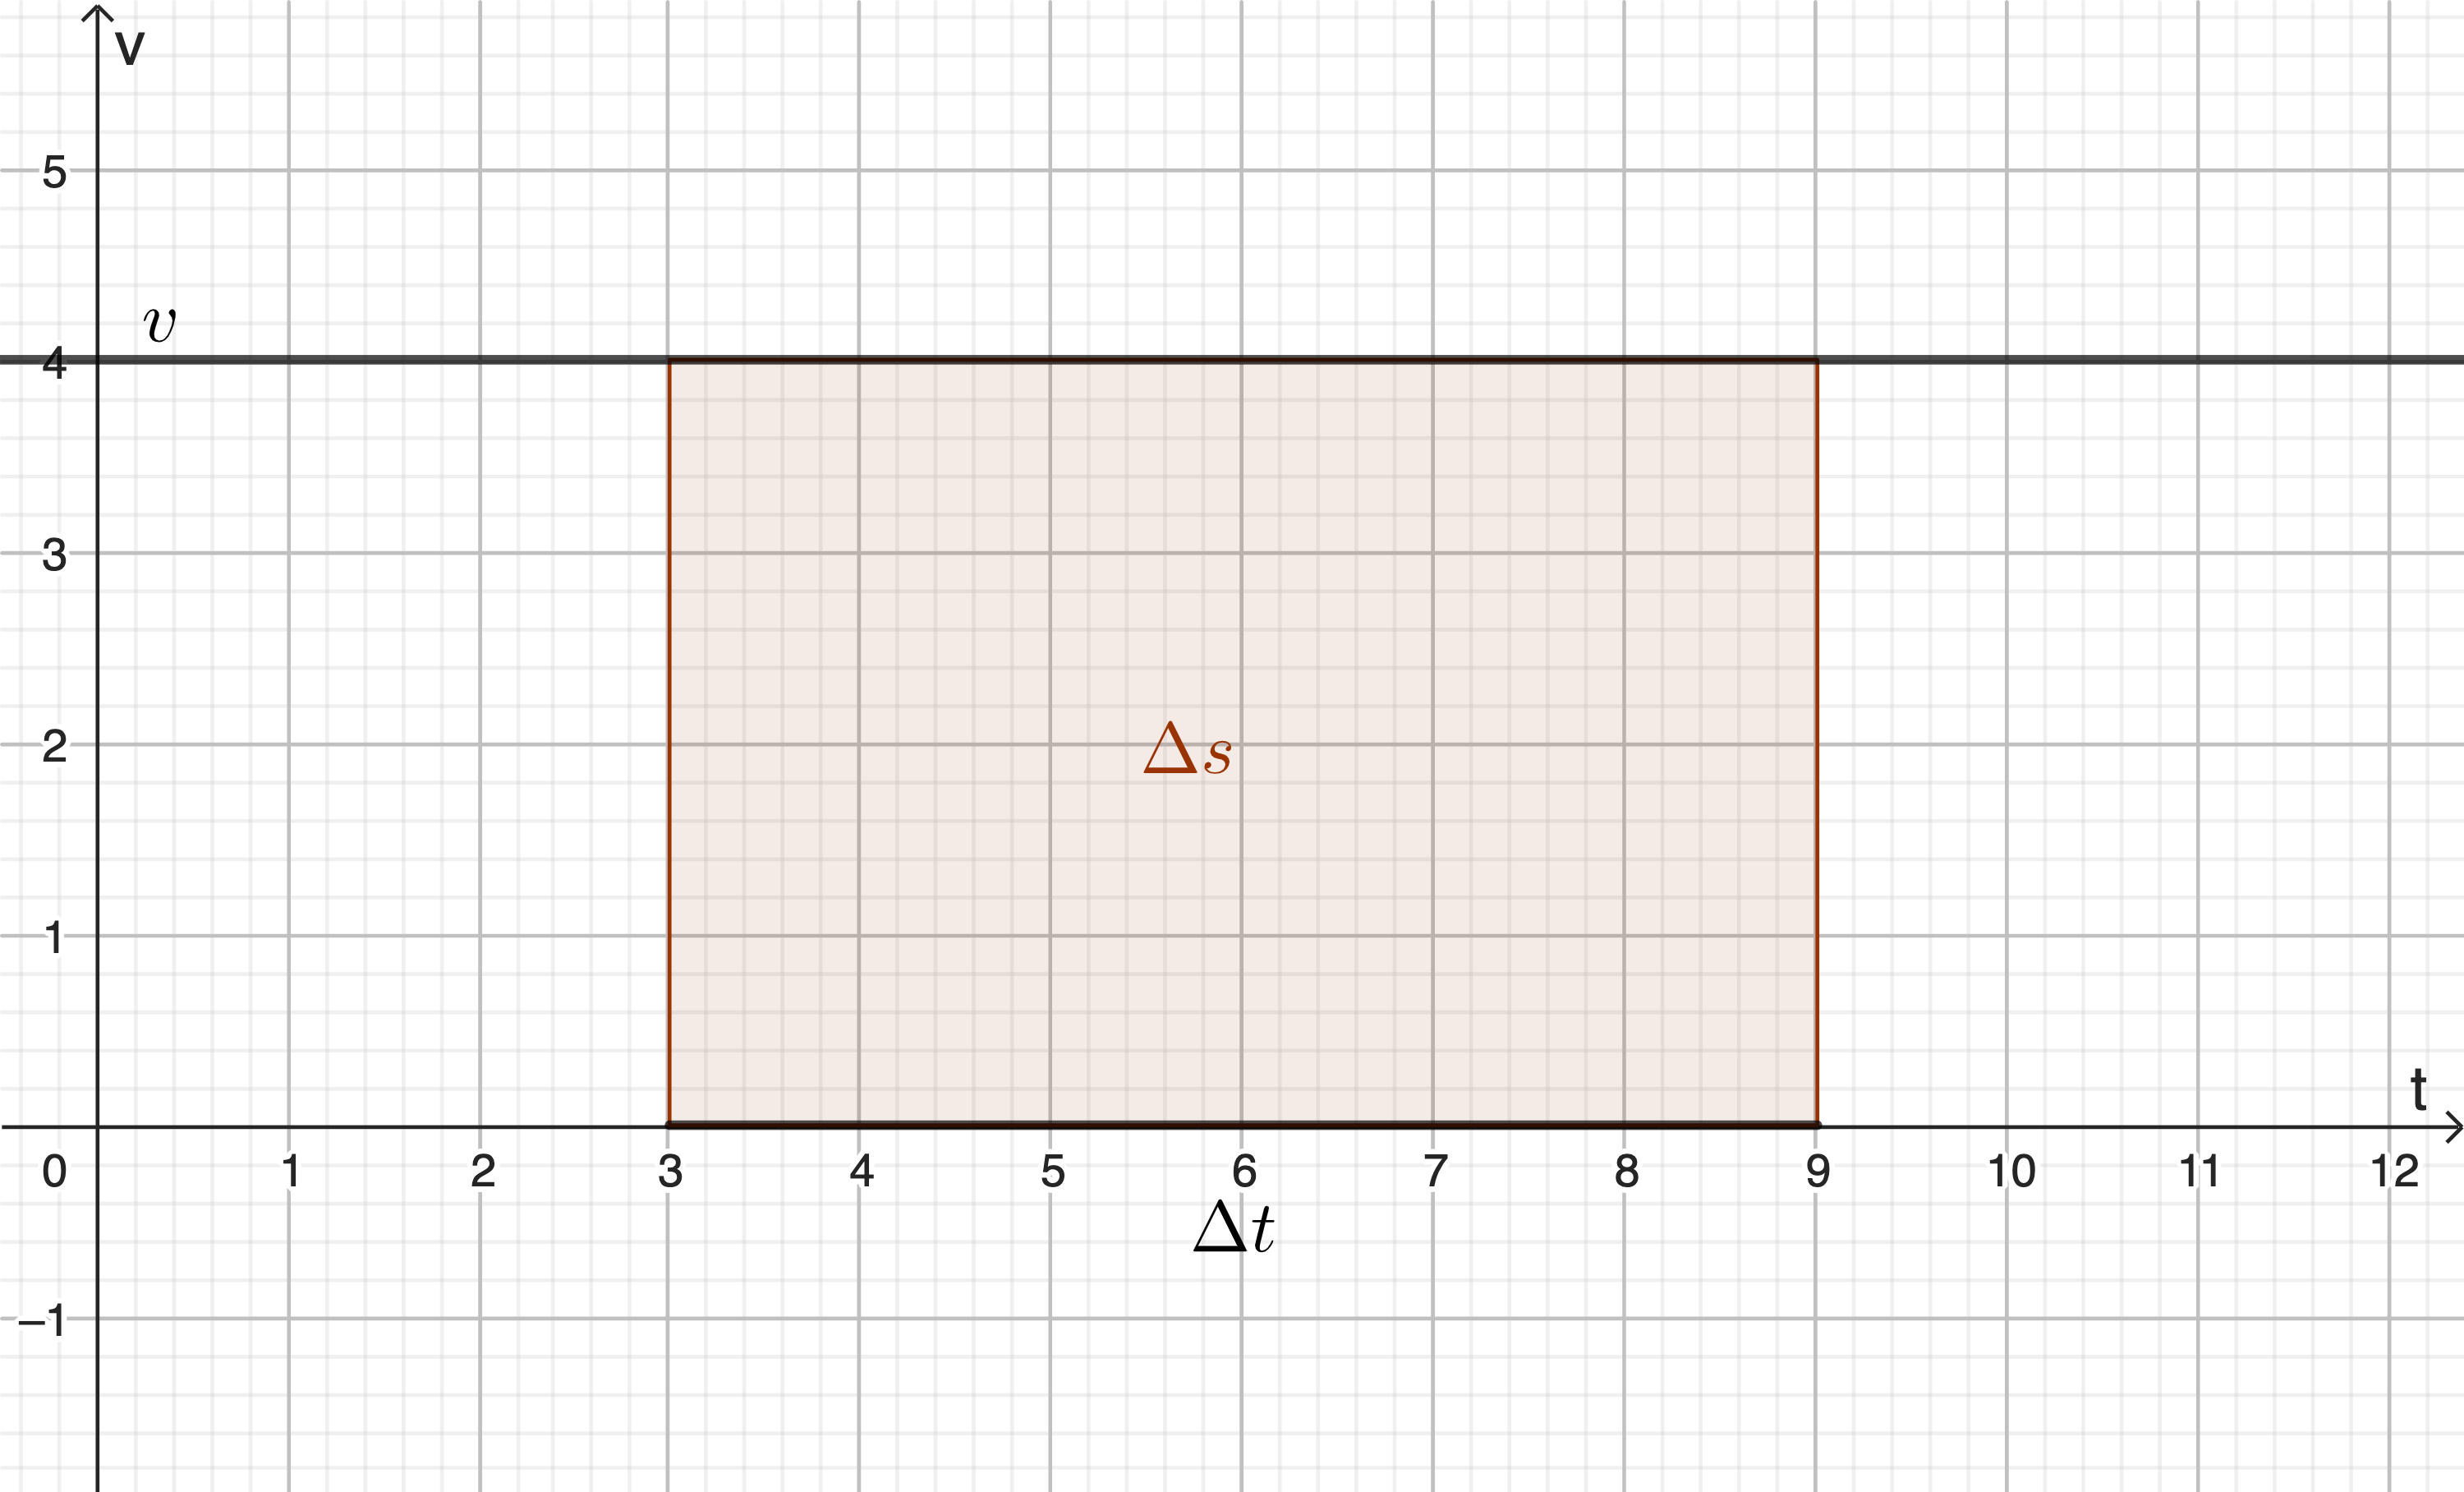
\includegraphics[width = 0.5\textwidth]{media/WegAlsIntegral1.png}
\end{center}

Etwas schwieriger wird es, wenn die Geschwindigkeit nicht konstant ist. Betrachten wir ein Körper, dessen Geschwindigkeit linear wächst: $v(t) = a\cdot t$. Welchen Weg legt der Körper im Zeitintervall $[t_1, t_2]$ zurück?

Um den zurückgelegten Weg näherungsweise zu berechnen, teilen wir das Zeitintervall $[t_1, t_2]$ in viele kleine Intervalle und nehmen an, dass in diesen kleinen Zeitintervallen die Geschwindigkeit näherungsweise konstant ist:
\begin{center}
    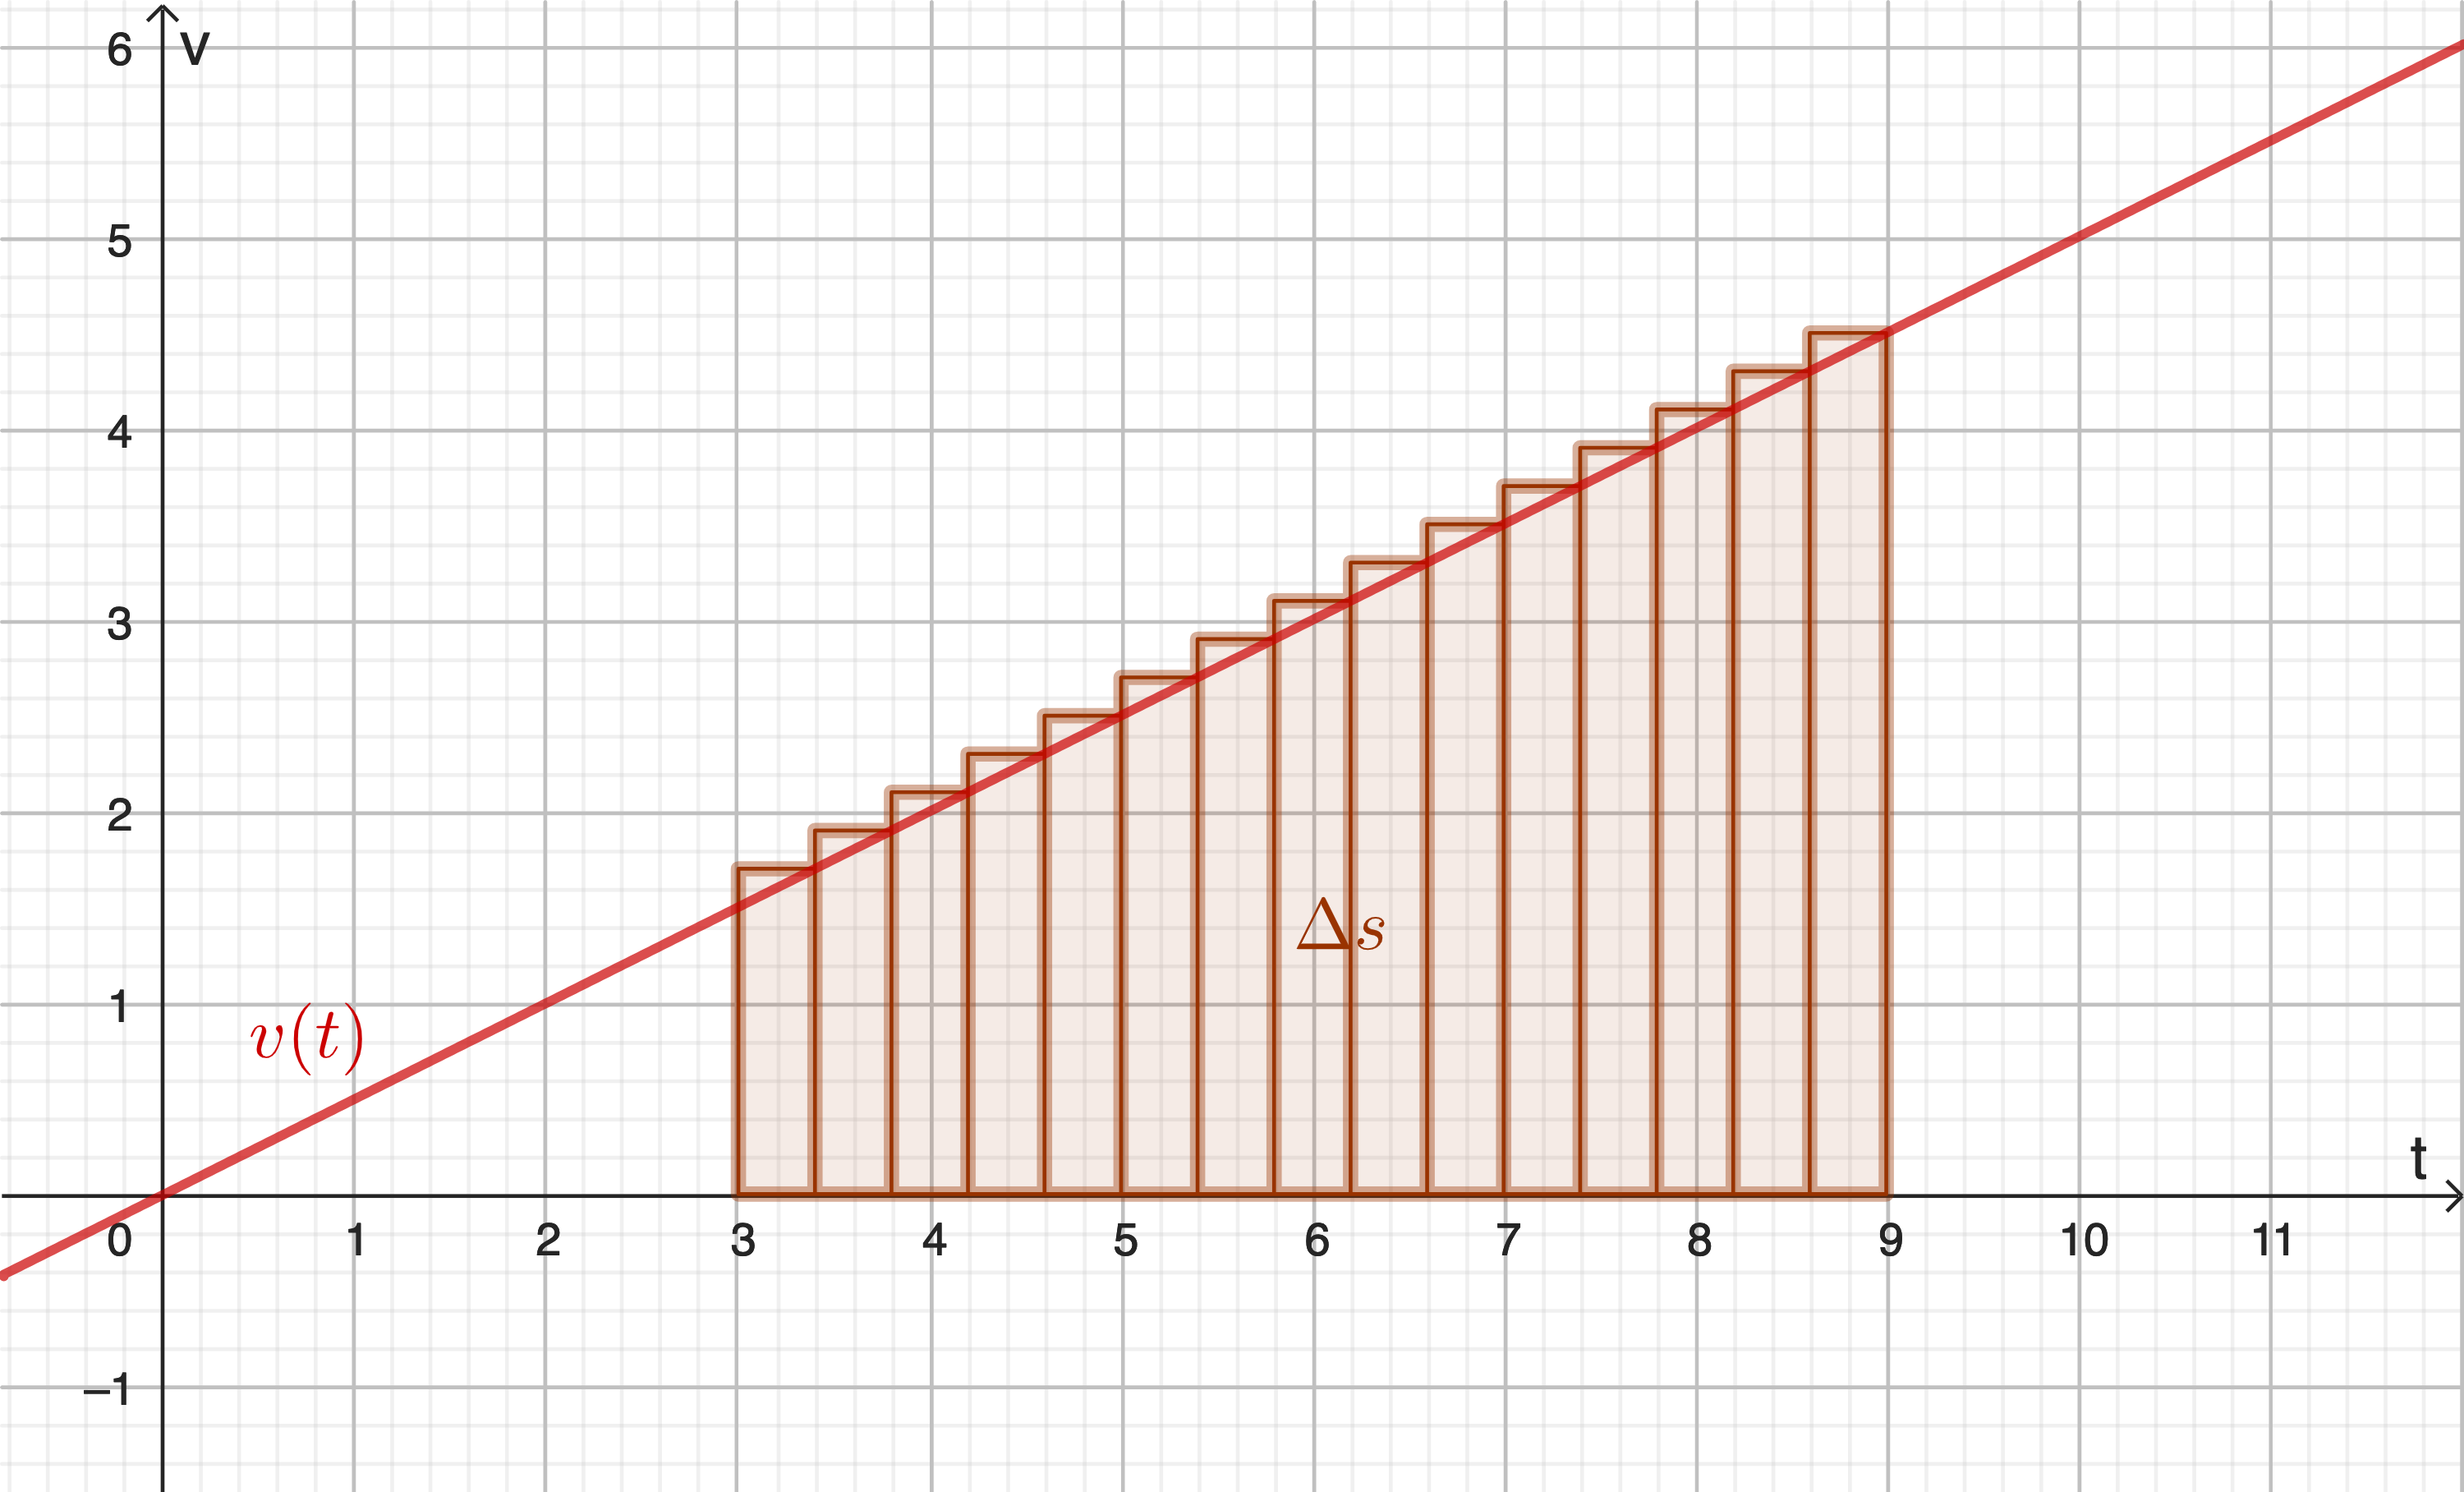
\includegraphics[width = 0.5\textwidth]{media/WegAlsIntegral2.png}
\end{center}
Diese Näherung ist umso besser, je kleiner und zahlreicher die Zeitintervalle werden. Im Grenzfall erhalten wir:
$$\Delta s = \int_{t_1}^{t_2} v(t) \,dt =  \int_{t_1}^{t_2} (a\cdot t) \,dt = \frac{1}{2}at_2^2-\frac{1}{2}at_1^2$$
 
\begin{satz}
    {Zurückgelegter Weg als Integral der Geschwindigkeit}{}
    Allgemein gilt:
    $$\Delta s = \int_{t_1}^{t_2} v(t) \,dt$$
\end{satz}

Die gleiche Überlegung stimmt auch für die mechanische Arbeit:

Die Energie, welche benötigt wird, um einen Körper gegen eine wirkende Kraft zu bewegen, wird in der Physik Arbeit genannt. Wenn die Kraft konstant ist, entspricht die Arbeit $W$ dem Produkt aus Kraft und Weg:
$W=F\cdot \Delta s$
\begin{bsp}
    {Arbeit bei konstanter Kraft}{}
    Welche Arbeit muss geleistet werden, um eine Masse $m$ von der Erdoberfläche auf die (geringe) Höhe $h$ zu bringen?

    Zurückgelegter Weg: \(\Delta s = h\)

    Wirkende Kraft (in der Nähe der Erdoberfläche): \(F = mg\)  mit $g \approx 9.81 m/s^2$

    Die Arbeit ist also
    \[W = mgh\]
    Die Arbeit entspricht gerade der potentiellen Energie einer Masse \(m\) auf der Höhe \(h\).
    Grafisch kann das Produkt aus Kraft und Weg wieder als Flächeninhalt interpretiert werden:
    \begin{center}
        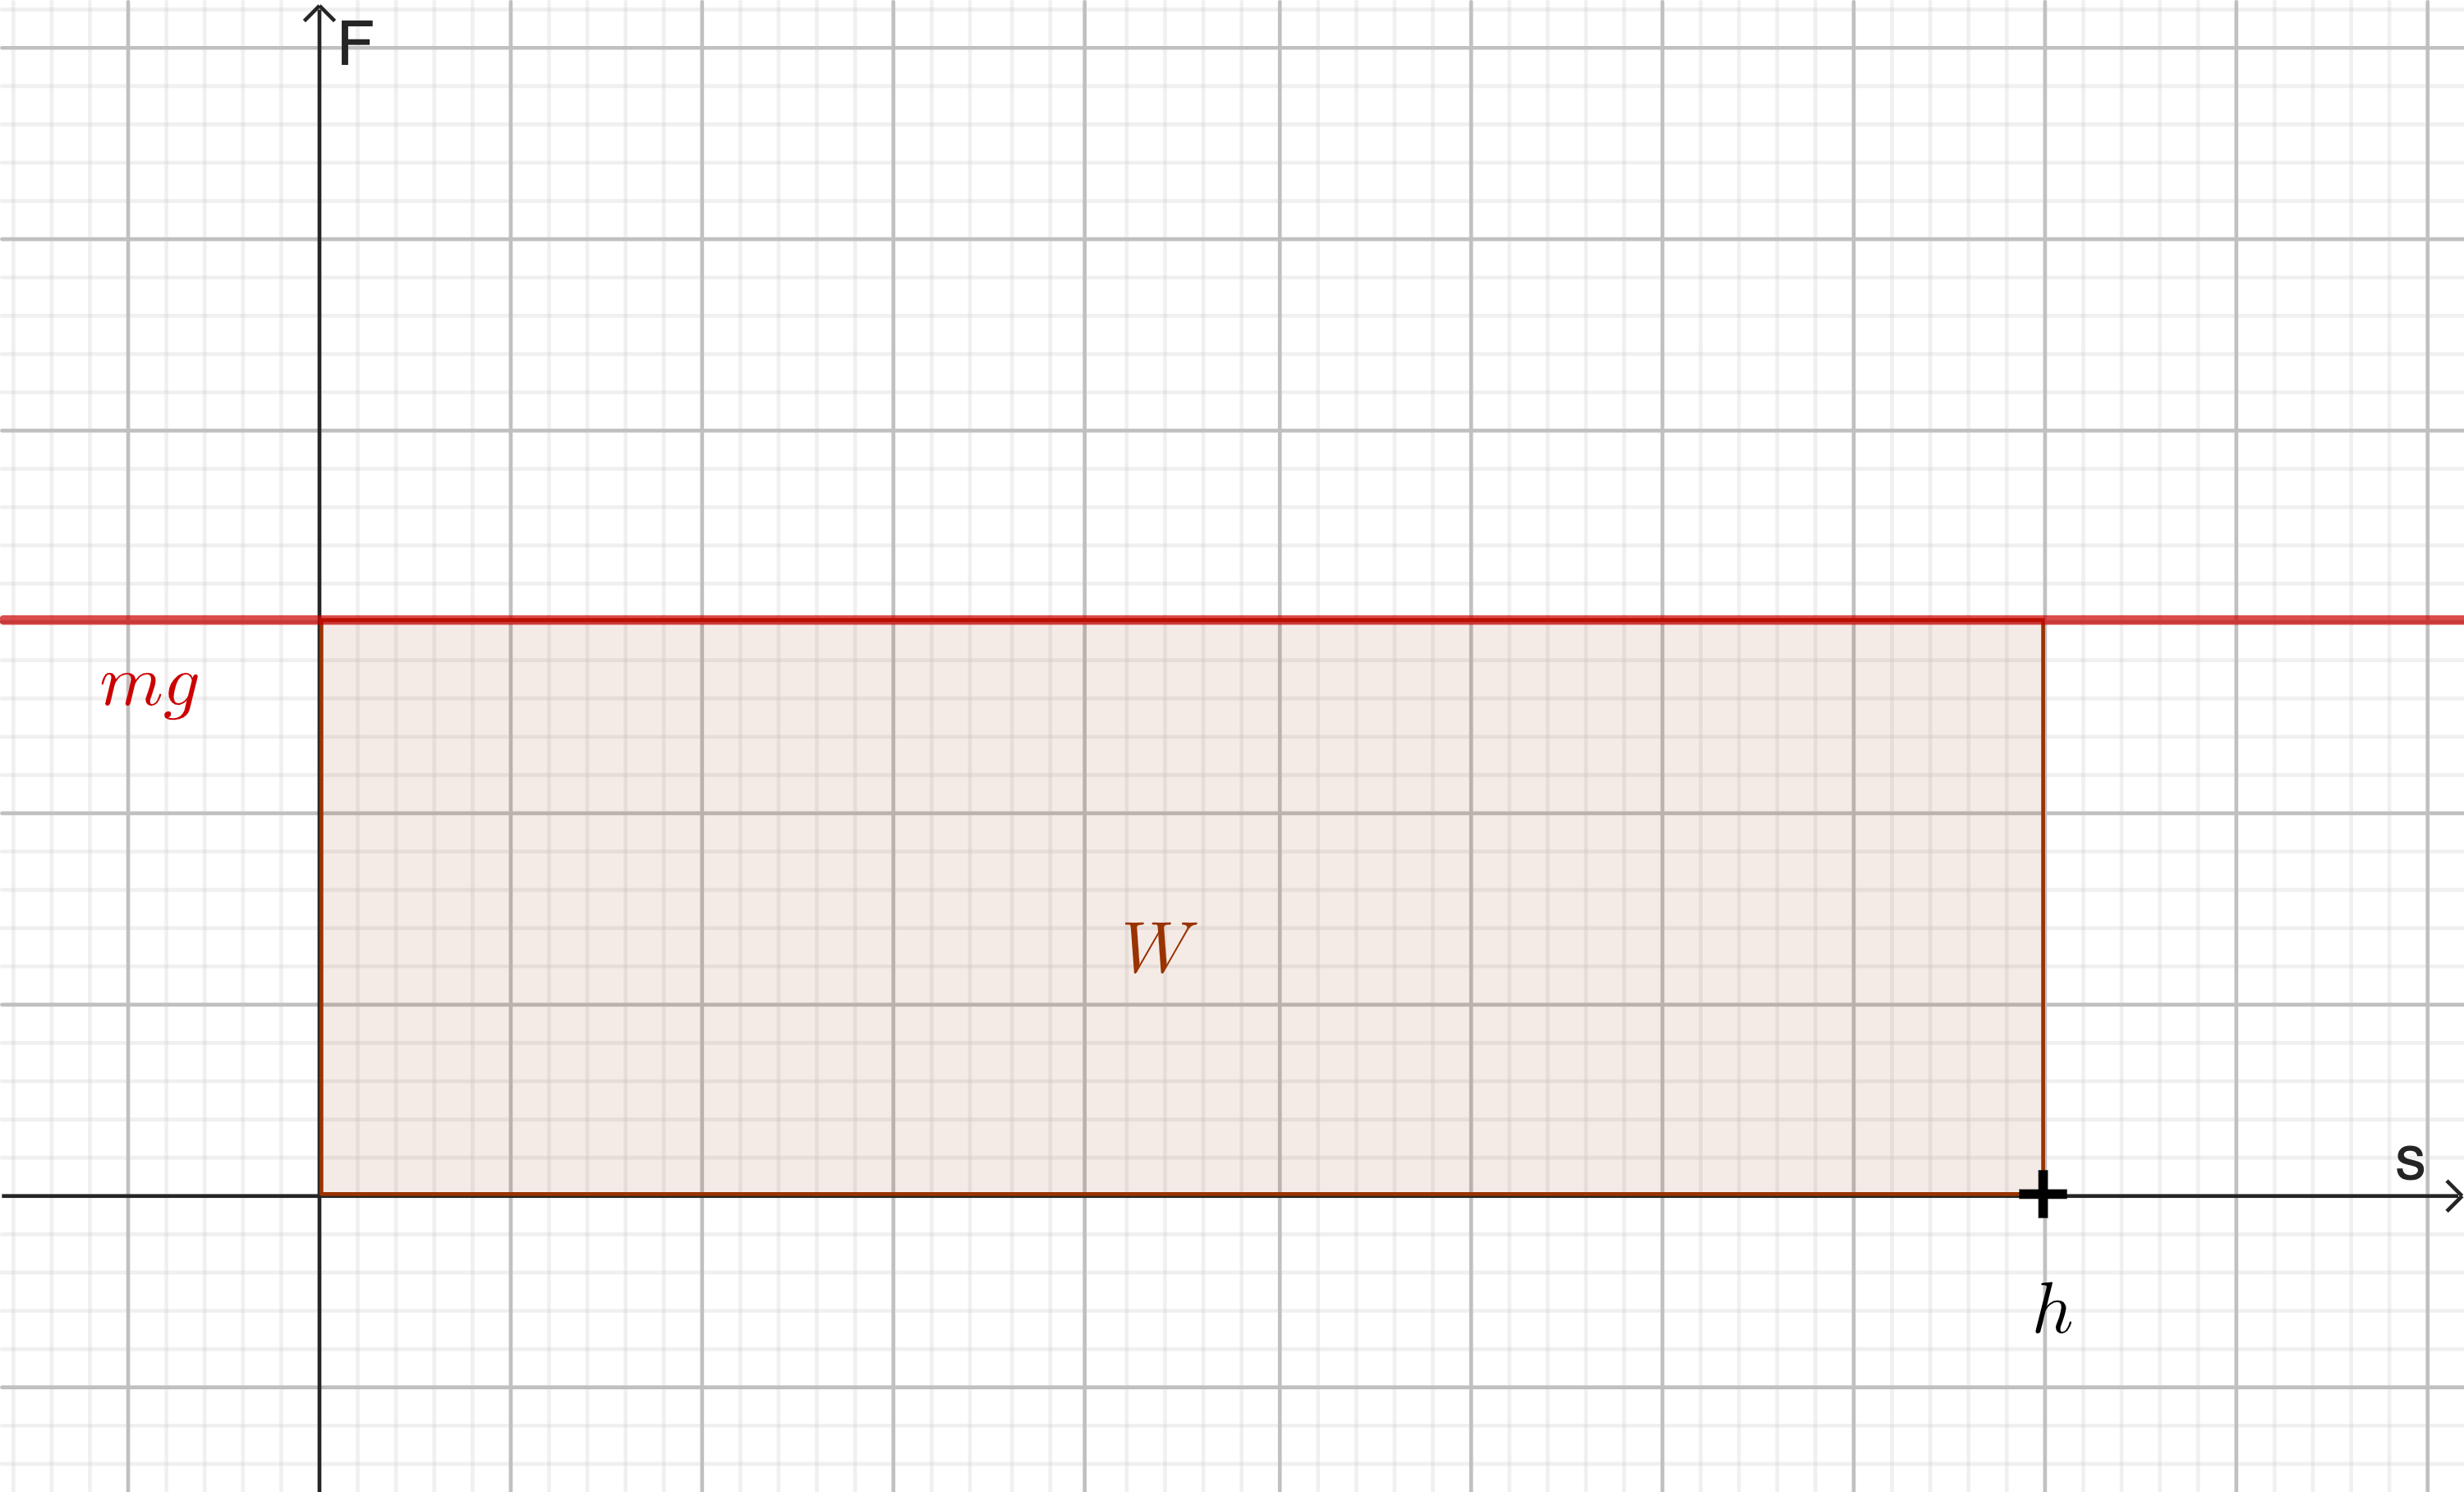
\includegraphics[width = 0.5\textwidth]{media/arbeitAlsIntegral1.png}
    \end{center}

\end{bsp}
\begin{bsp}
    {Arbeit bei linear wachsender Kraft}{}
    Eine Feder mit der Federkonstante \(k\) wird aus der Ruhelage um die Strecke \(a\) gespannt. In diesem Beispiel ist die wirkende Kraft \(F\) proportional zur Auslenkung \(x\) der Feder: \(F = k \cdot x\), wobei $k$ die Federkonstante ist. Um die Arbeit näherungsweise zu berechnen, teilen wir die Strecke \(\Delta s = a\) in viele kleine Intervalle und nehmen an, dass in diesen kleinen Wegintervallen die wirkende Kraft näherungsweise konstant ist.

    \begin{center}
        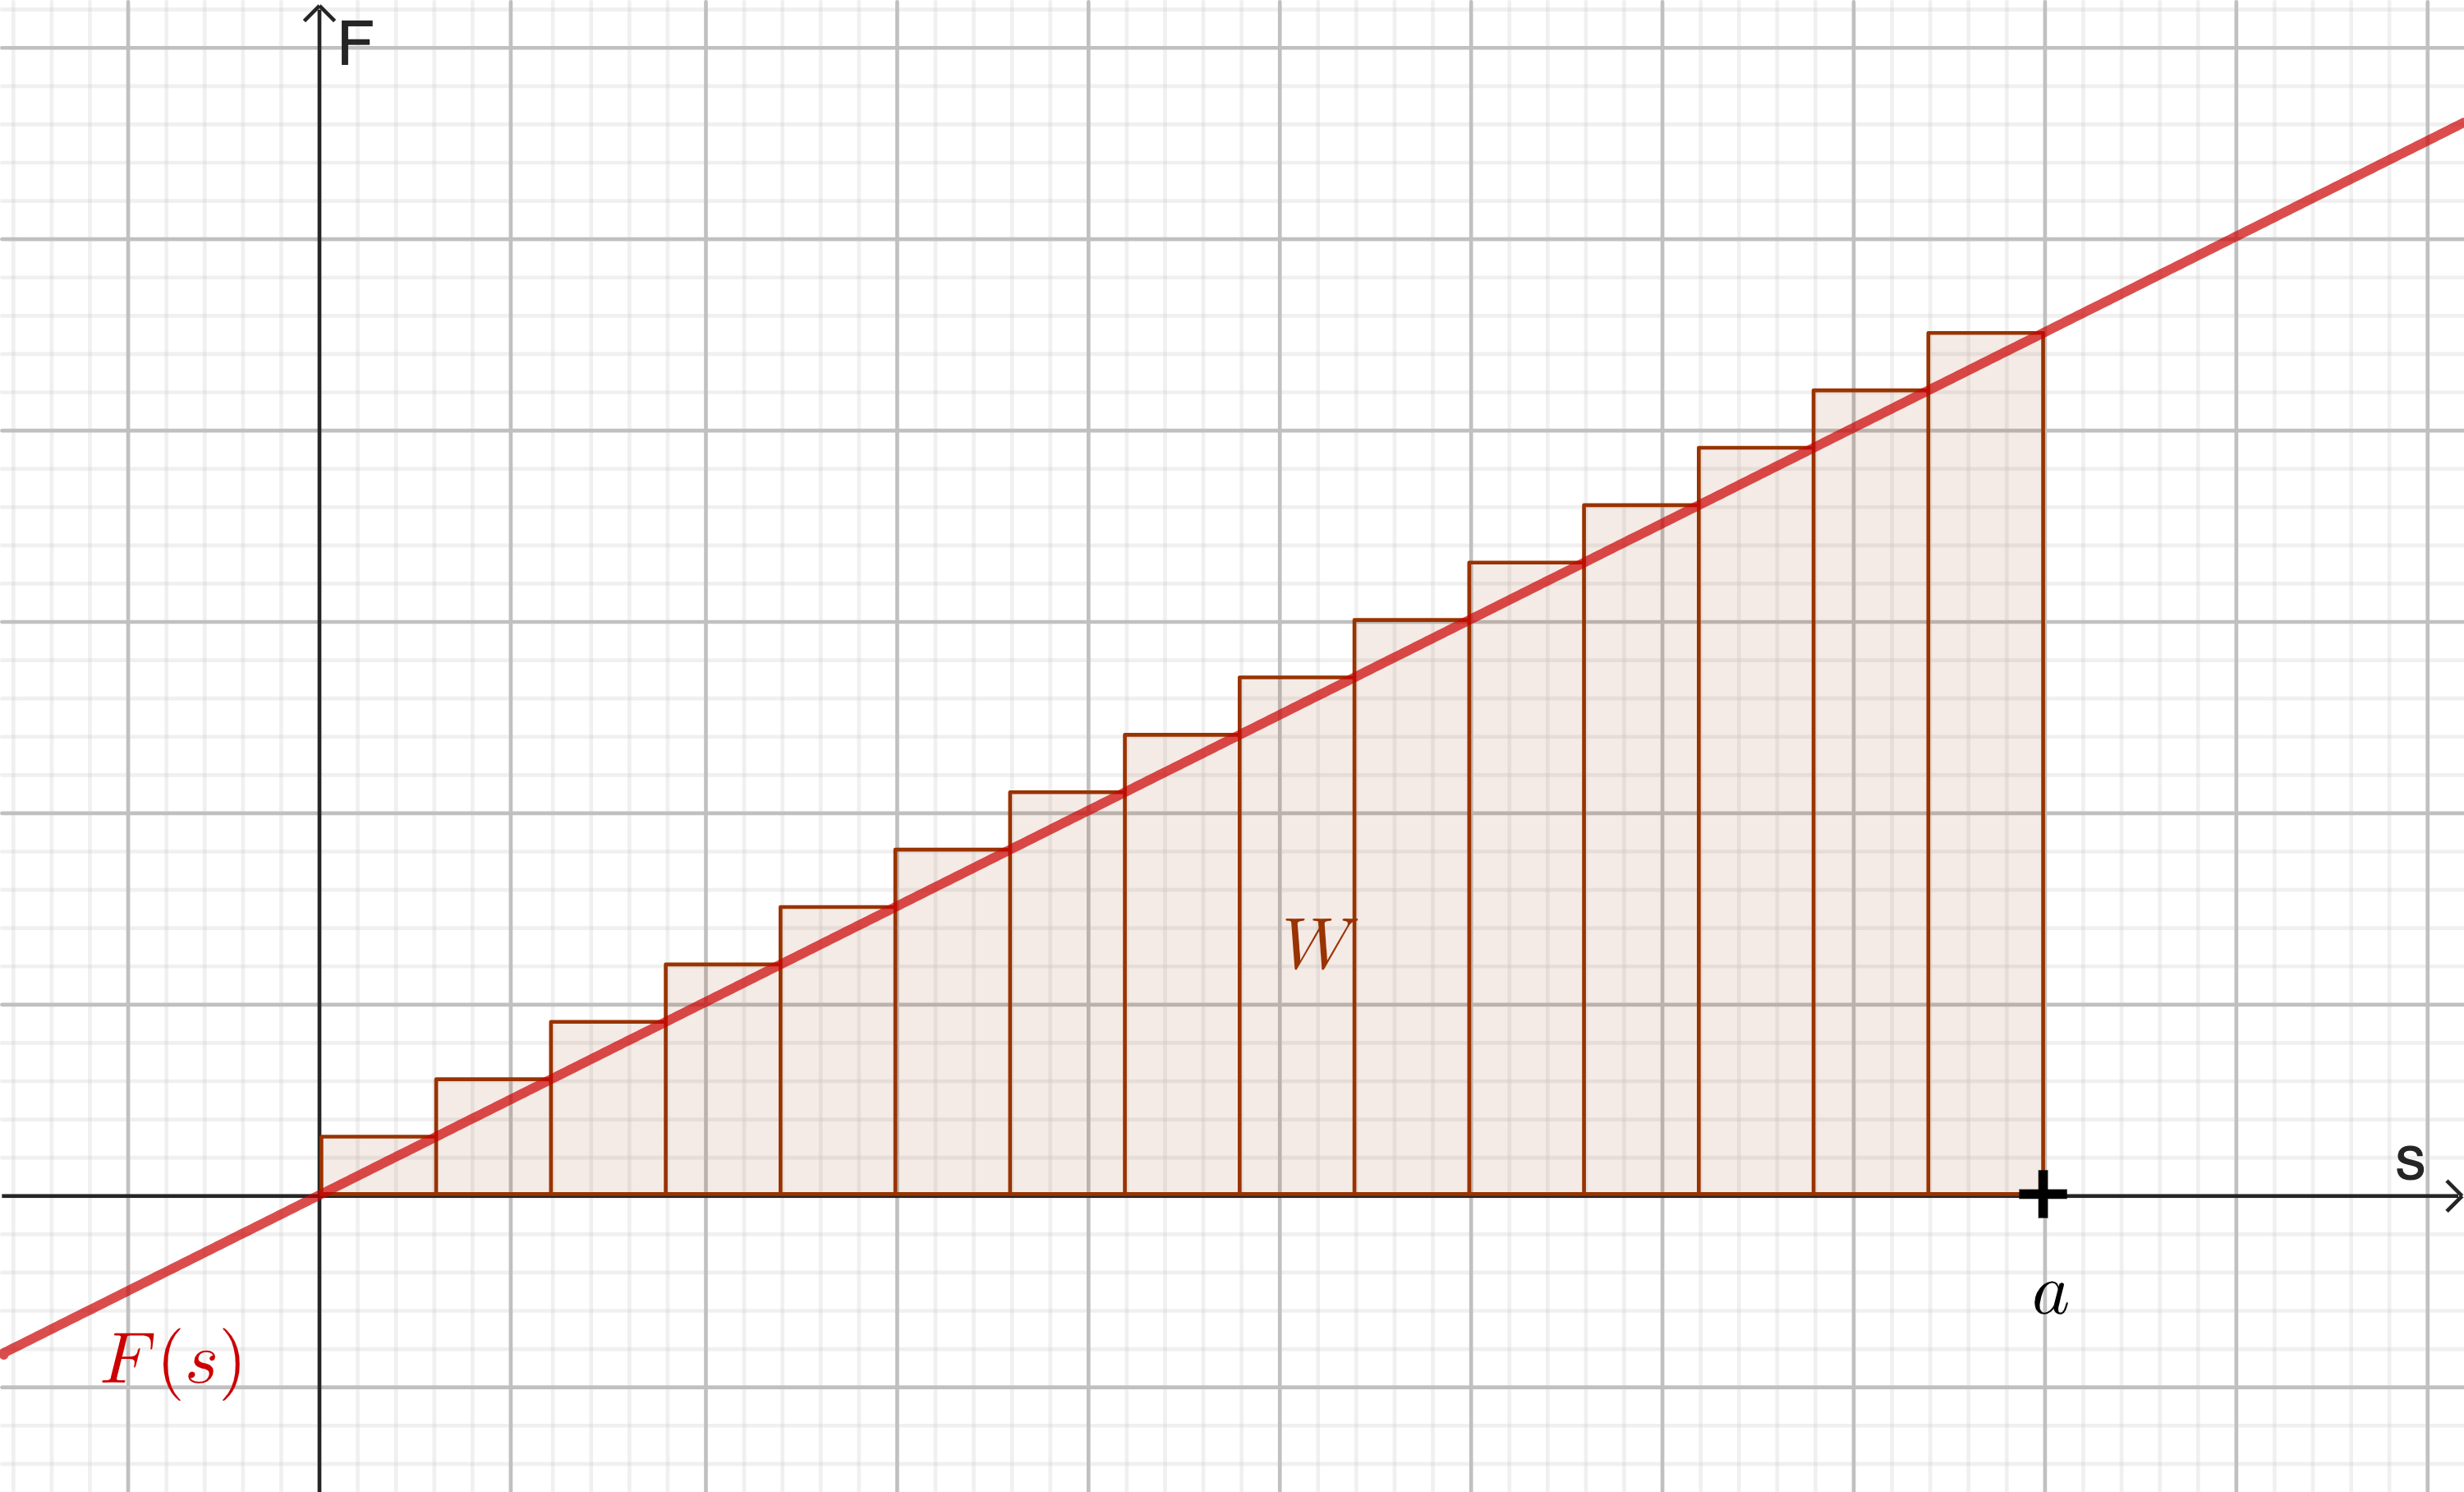
\includegraphics[width = 0.5\textwidth]{media/ArbeitAlsIntegral2.png}
    \end{center}

    Diese Näherung wird umso besser, je kleiner und zahlreicher die Wegintervalle werden. Im Grenzfall erhalten wir:
    \[ W = \int_{0}^{a} F(s) \, ds = \frac{k}{2} a^2 \]

\end{bsp}
\begin{satz}
    {Mechanische Arbeit als Integral}{}
    Allgemein gilt
    $$W = \int_{s_1}^{s_2} F(s) \, ds$$
\end{satz}

\clearpage
\section{Differentialgleichungen}
Dieses Thema wird im Schwerpunktfach behandelt.
\section{Weitere Themen}
\subsection*{Integrationstechniken}
Wie wir gesehen haben, bilden die Stammfunktionen den Schlüssel zur Berechnung Integralen, die in vielfältigen Anwendungssituationen eine wichtige Bedeutung haben Umso einschränkender ist es, dass wir im Moment nur von ganz wenigen, einfachen Funktionen die Stammfunktion angeben können. Zum Beispiel:
\[
\int x\sqrt{x} \,dx = \frac{2}{5}x^{5/2} + c
\]
\[
\int e^x \,dx = e^x + c
\]
\[
\int \frac{1}{x} \,dx = \ln(|x|) + c
\]
\[
\int \sin(x) \,dx = -\cos(x) + c
\]

Sobald die Funktion ein klein wenig komplizierter wird, ist das Auffinden der Stammfunktion nicht mehr so einfach. Zum Beispiel
\[
\int x \cdot \cos(x) \,dx = ?
\]
In diesem Kapitel werden Sie Techniken kennenlernen, mit denen man in einigen Fällen die Stammfunktion bestimmen kann.

Diese Techniken haben gemeinsam, dass Sie gewissermassen eine Ableitungsregel umgekehrt anwenden. Eine dieser Techniken, haben Sie bereits kennengelernt: Die \emph{lineare Substitution}.

\begin{bsp}
    {Eine lineare Substitution}{}
    $$\int \cos(3x-1) \, dx = \sin(3x-1) \cdot \frac{1}{3} + C$$
\end{bsp}

Die linearen Substitution ist so etwas, wie die Kettenregel der Integration. Im Folgenden  werden wir uns mit Produkten von Funktionen befassen und eine Art ``Produktregel der Integration' kennenlernen.

\begin{LA}
    {Versuch und Irrtum}{}
    Finden Sie eine Stammfunktion von $f(x) = x\cdot \cos(x)$, indem Sie Kandidaten ausprobieren und laufend verbessern.
\end{LA}
 
\clearpage
\begin{satz}
    {Die partielle Integration}{}
    Sei $F$ eine Stammfunktion von $f$. Dann gilt
    $$ \int f(x)\cdot g(x) \, dx = F(x)\cdot g(x) - \int F(x) \cdot g'(x) \, dx$$
\end{satz}

\begin{proof}
    
    \vspace*{3cm}
\end{proof}

\begin{bsp}
    {}{}
    $\int x\cdot \cos(x) \, dx = $
    \vspace*{2cm} 
\end{bsp}
\begin{bsp}
    {}{}
    $\int x^2 \cdot \cos(x) \, dx= $
    \vspace*{6cm} 
\end{bsp}

\begin{bsp}
    {}{}
    $\int \ln(x) \, dx= $
    \vspace*{4cm} 
\end{bsp}

\begin{bsp}
    {}{}
    $\int \cos^2(x) \, dx= $
    \vspace*{8cm} 
\end{bsp}
\begin{ueb}
    {}{}
    Im Buch auf Seite 161 und 162.
    Zusätzlich
    \begin{enumerate}
        \item Berechnen Sie den Inhalt der Fläche zwischen dem Graphen von $f(x) = (x-2)\cdot e^{0.5x}$, der $x$ Achse und der Geraden $g: \: x=0$.
        
        (Lösung 2.87)
        \item Das Kurvenstück der Funktion $f:\: x\mapsto xe^x$, das zwischen Nullstelle und Extremum liegt, rotiert um die $x$-Achse. Berechnen Sie das Volumen des Rotationskörper
        
        (Lösung 0.25)
    \end{enumerate}
\end{ueb}
\clearpage
\subsection*{Nicht-lineare Substitution}
Mit der linearen Substitution können wir die Stammfunktion von Funktionen der Form $f(ax+b)$ bestimmen. Man kann das auch so betrachten, dass wir Funktionen der Form $f(u(x))$ integriert haben, wobei $u(x)=ax+b$ eine lineare Funktion ist. In diesem Abschnitt möchten wir der Frage nachgehen, was passiert, wenn $u(x)$ nicht linear ist. Dazu betrachten wir zunächst die andere Richtung: die Ableitung. Sei $F(x)$ eine Stammfunktion von $f(x)$. Dann gilt nach der Kettenregel:
$$\left( F(u(x)) \right)' = f(u(x)) \cdot u'(x)$$
Das lässt sich auch so formulieren:
\begin{satz}
    {Nicht-lineare Substitution}{}
    Sei $F(x)$ eine Stammfunktion von $f(x)$. Dann gilt

\[
\int f(u(x)) \cdot u'(x) \, dx = F(u(x))
\]

\end{satz}

Diesen Satz kann man sich gut merken, wenn man die Schreibweise $\frac{d}{dt}$ für die Ableitung nach $t$ verwendet:

\begin{satz}
    {Substitution in Kurzform}{}
    \[
\int f(u) \frac{du}{dt} \, dt = \int f(u) \, du
\]

\end{satz}
So wird deutlich, woher der Name „Substitution“ kommt: Man ersetzt die Variable, nach der integriert wird.

Die Schwierigkeit in der Anwendung besteht darin, die Funktion $f(u)$ und $u(x)$ zu erkennen. Betrachten Sie das folgende 

\begin{bsp}
    {Wird in der Klasse ergänzt}{}
    \[
\int \frac{1-x}{\sqrt{2x-x^2}} \, dx = ?
\]
\end{bsp}
\clearpage
\subsection*{Nicht elementar integrierbare Funktionen}
Die erlernten Integrationstechniken erwecken vielleicht den Eindruck, dass zu jeder Funktion unter Zuhilfenahme einer geeigneten Technik eine Stammfunktion ermittelt werden kann. Das stimmt aber nicht ohne Weiteres. Um diese Aussage zu verstehen, führen wir den Begriff der elementaren Funktionen ein:
\begin{definition}
    {Elementare Funktionen - eine mögliche Definition}{}
    Eine Funktion heisst \emph{elementar}, wenn sie eine Verkettung von (endlich vielen) Polynom-, Potenz-, trigonometrischen, Exponential- und Logarithmusfunktionen ist.\footnote{Es gibt allerdings keine allgemeingültige, präzise Definition von elementaren Funktionen}
\end{definition}
Fast alle Funktionen, die wir bis jetzt betrachtet haben, gehören zu dieser Klasse von Funktionen. Das hat damit zu tun, dass wir Funktionen meist durch Ihre Gleichung angeben. Damit sind sie automatisch eine Summe, Produkt oder Verkettung der bekannten Funktionstypen und somit elementar. Hinzu kommt, dass auch die Ableitung einer elementaren Funktion wieder elementar ist. Beim Integrieren ist das nicht der Fall!
\begin{bsp}
    {eine Funktion, die nicht elementar integrierbar ist}{}
    $$f(x) = \frac{1}{2\pi} e^{-\frac{1}{2}x^2}$$
    \begin{center}
        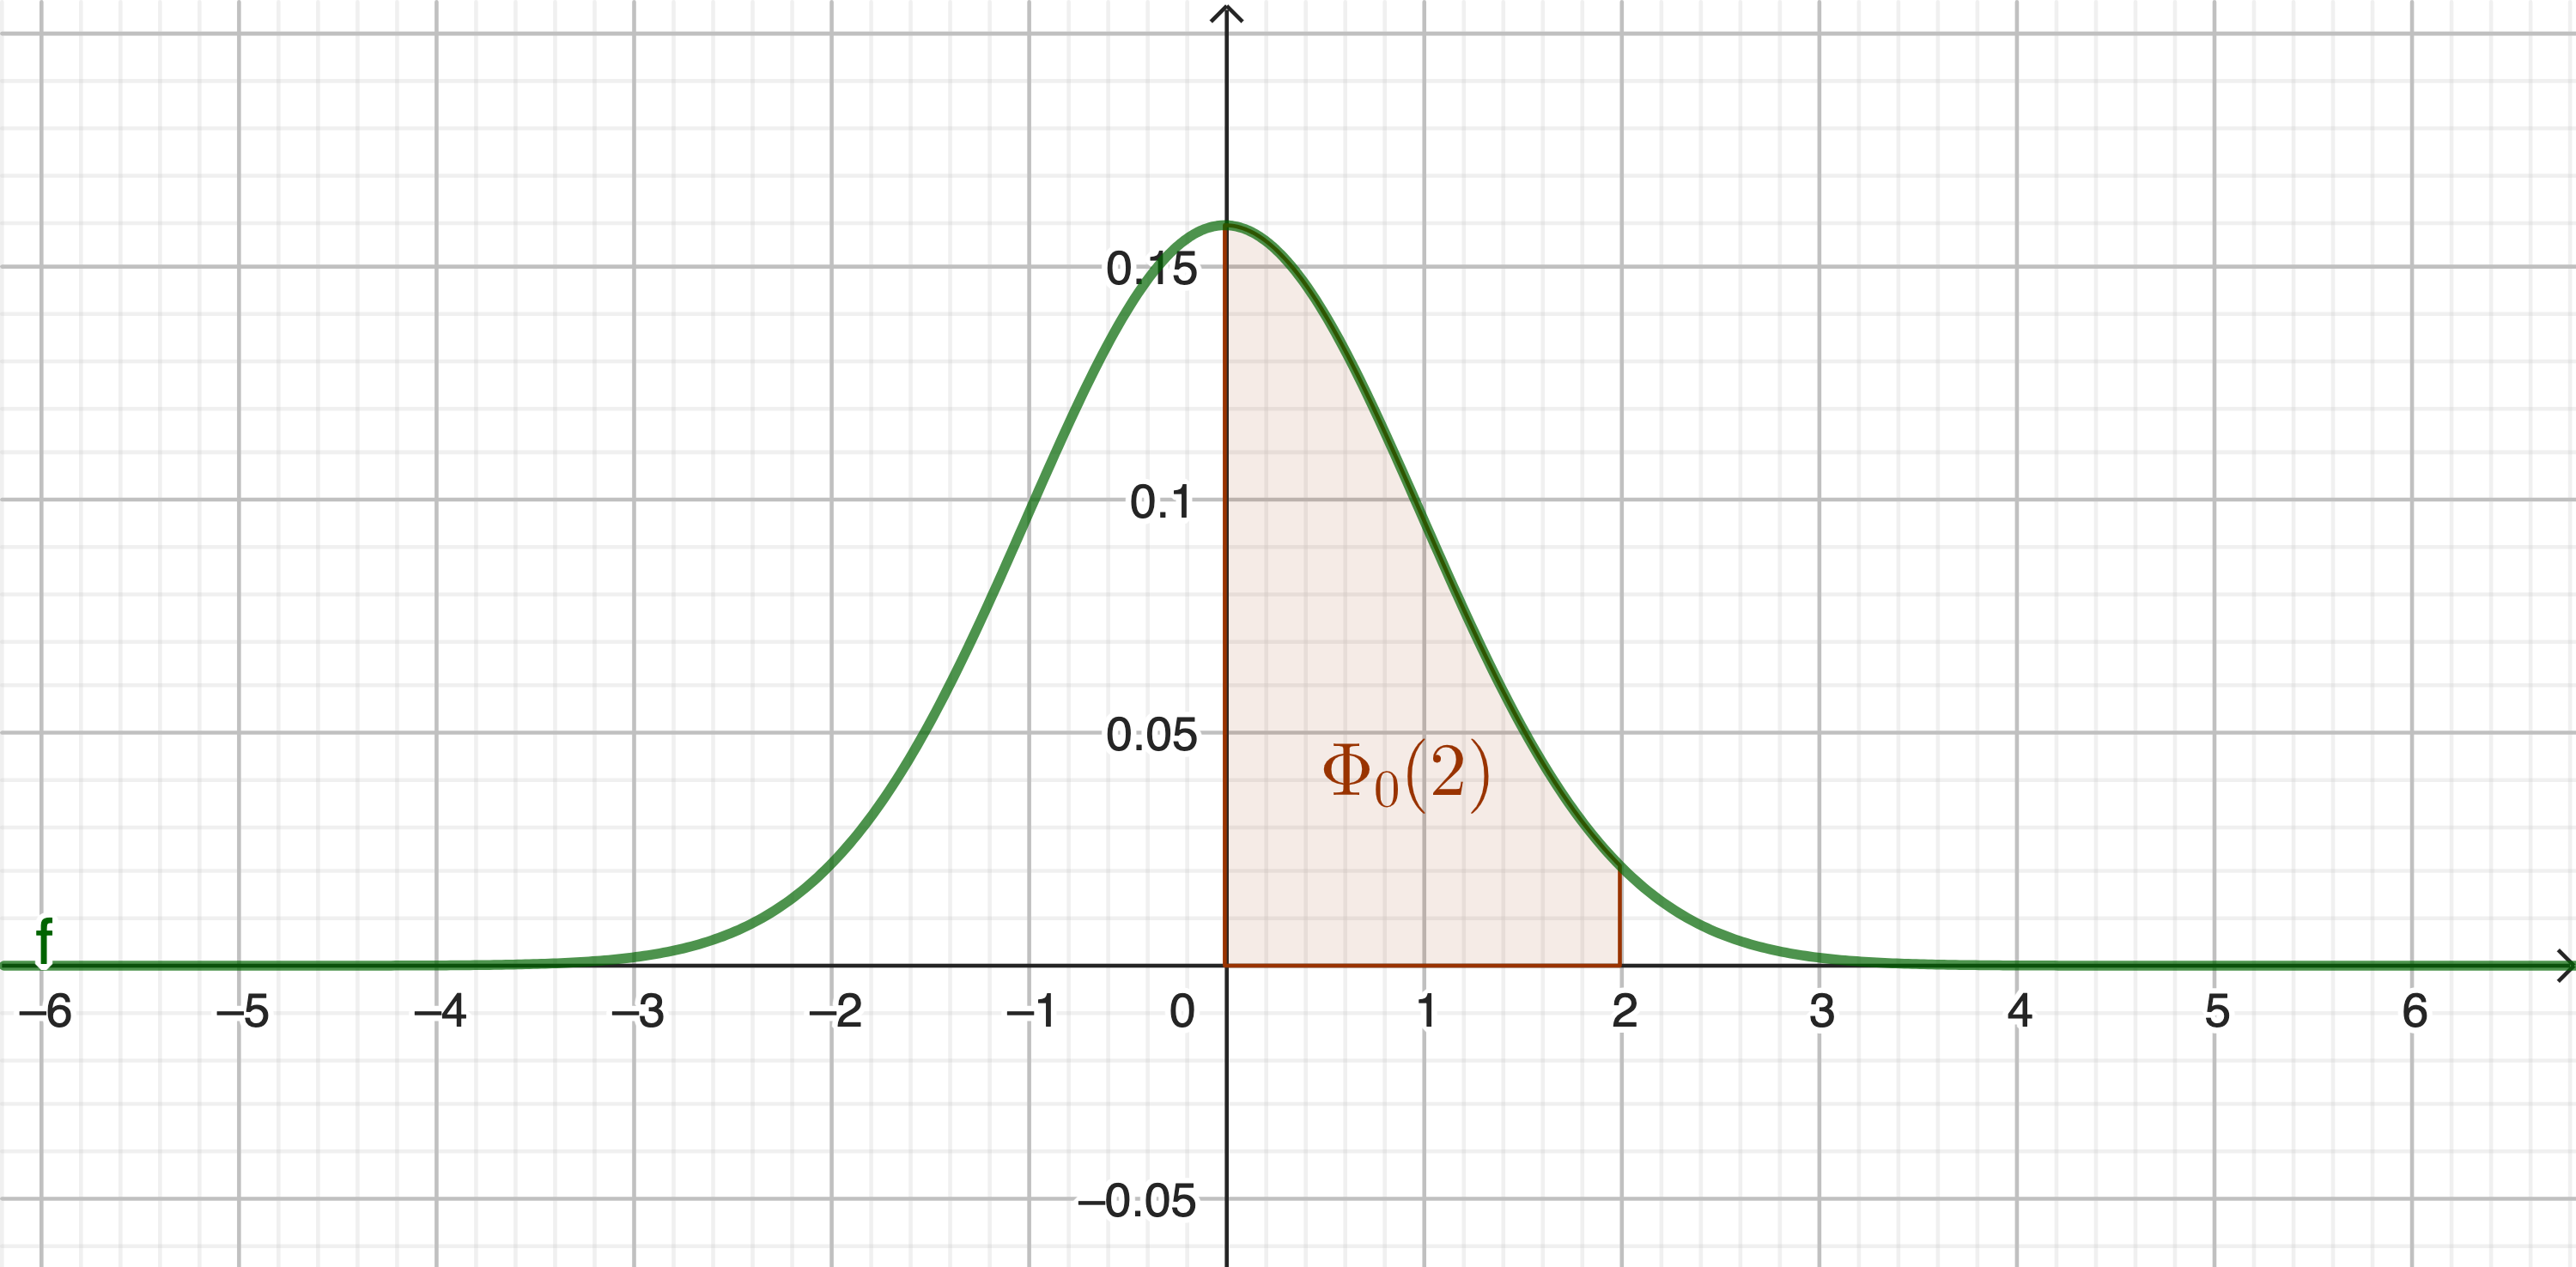
\includegraphics[width = 0.5\textwidth]{media/Glockenkurve.png}
    \end{center}

    Der Graph von $f$ wird auch Gauss'sche Glockenkurve genannt und ist in der Wahrscheinlichkeitsrechnung sehr wichtig. Die Funktion 
\[
\Phi_0 (t) = \int_0^t f(x) \, dx
\]
ist wohldefiniert, gehört aber nicht zur Klasse der elementaren Funktionen. Die Werte von $\Phi_0$ kann man näherungsweise bestimmen – zum Beispiel indem man die entsprechende Fläche durch die Ober- bzw. Untersumme approximiert.


\end{bsp}











\end{document}